\documentclass[12pt,addpoints, answers, fleqn]{exam} 

\RequirePackage[colorlinks, hyperindex, plainpages=false]{hyperref}

\usepackage{graphicx,type1cm,eso-pic,color}
\usepackage{comment}
\usepackage{versions} 

\newcommand*\Heq{\ensuremath{\overset{\kern2pt H}{=}}}

%--------VERSION CONTROL SETTINGS---------------------
%--------VERSION CONTROL SETTINGS---------------------
%--------VERSION CONTROL SETTINGS---------------------
%--------VERSION CONTROL SETTINGS---------------------
%--------VERSION CONTROL SETTINGS---------------------
%--------VERSION CONTROL SETTINGS---------------------
%--------VERSION CONTROL SETTINGS---------------------


\excludecomment{teacher} %This should be turned on when printing for student
%\includecomment{teacher} %This should be turned on when printing for teacher

%--------VERSION CONTROL SETTINGS---------------------
%--------VERSION CONTROL SETTINGS---------------------
%--------VERSION CONTROL SETTINGS---------------------
%--------VERSION CONTROL SETTINGS---------------------
%--------VERSION CONTROL SETTINGS---------------------
%--------VERSION CONTROL SETTINGS---------------------
%--------VERSION CONTROL SETTINGS---------------------

\usepackage{cancel}

%\makeatletter
%          \AddToShipoutPicture{
%            \setlength{\@tempdimb}{.5\paperwidth}
%            \setlength{\@tempdimc}{.5\paperheight}
%            \setlength{\unitlength}{1pt}
%            \put(\strip@pt\@tempdimb,\strip@pt\@tempdimc){
%        \makebox(0,0){\rotatebox{55}{\textcolor[gray]{0.85}
%        {\fontsize{5cm}{5cm}\selectfont{draft}}}}
%            }
%        }
\makeatother
\usepackage{graphicx}
\usepackage{amssymb}
\usepackage{amsmath}
\usepackage{wasysym}
\usepackage{url}
\usepackage{color}

\shadedsolutions 
\definecolor{SolutionColor}{rgb}{0.8,0.9,1.0} 
%\CorrectChoiceEmphasis{\color{rgb}{0.8,0.9,1}} 


\pagestyle{headandfoot} 

\begin{document}

\runningheadrule 
\header{Calculus I\\MTH-121}{\textbf{Essex County College\\Division of Mathematics}}{LMS Project\\Class Notes} 

\firstpagefooter{\url{ron.bannon@mathography.org}}{}{\LaTeXe}
\runningfootrule
\runningfooter{}{Page \thepage\ of \numpages}{} 

\tableofcontents

\vfill
\pagebreak

\begin{center} 
\fbox{
\fbox{
\parbox{5.5in}
{Errors in this document should be reported to Ron Bannon.
\begin{center}
\url{ron.bannon@mathography.org}
\end{center}
This document \emph{may} be shared with Essex County College students and instructors only.}}}
\end{center} 

\vfill
\pagebreak



%*-*-*-*-*-*-*-*-*-*-*-*-*-*-*-*-*-*-*-*-*-*-*-*-*-*-*-*-*-*-*-*-*-*-*-*-*-*-*-*-*-*-*-*-*-*-*-*-*-*-*-*-*-*-*-*-*-*-*-*-*-*-*-*-*-*-*-*-*-*-*-*-*-*-*-*-*-*-*-*-*-*-*-*-
\section{Review}
It is absolutely imperative that you have a fairly good grasp of the mathematics covered in prior ECC mathematics courses including Algebra (MTH-100) Pre-Calculus I and II (MTH 119-120). You may visit
\begin{description}
\item[MTH 100:] \url{http://mth100.mathography.org/}
\item[MTH 119:] \url{http://mth119.mathography.org/}
\item[MTH 120:] \url{http://mth120.mathography.org/}
\end{description}
to see what materials are covered in these three courses. Although your teacher may spend some time in class  discussing material covered in prior mathematics courses, you can not expect that this pre-requisite materials will be covered sufficiently well enough to remediate inadequate preparation. Being prepared is the first step!

\vfill
\pagebreak




\section{Course Web Page}
Please visit \url{http://mth121.mathography.org/} to learn more about how this course will be run. On this website you will be able to view the course outline, section specific syllabi,  this guide,\footnote{This is what I'd like my notes to look like If I were a student in this class. You should make some attempt to write your own notes, or at least annotate these. Please try to follow what is being done in class, and do not do the homework until you understand what was done in class.} and information about accessing online homework. Visit this page often!

\vfill
\pagebreak

\section{This Guide}
This guide is being provided as a way to structure MTH 121 across sections and semesters. Section headings that follow correspond to actual WebAssign assignments, and the material in these sections address materials in these assignments.  This guide is not a textbook and it should not be used as such---it just provides \emph{structure} for  teachers and students.

\begin{enumerate}
\item Please come to all classes, these notes are not to be used as an excuse not to attend.
\item These notes will not be read as a script, but teachers/students are encouraged to follow the content of these notes. However, your teacher may or may not do all the problems that are in the notes. You should  make every attempt to follow what your teacher is doing in class.
\end{enumerate}



\vfill
\pagebreak



%*-*-*-*-*-*-*-*-*-*-*-*-*-*-*-*-*-*-*-*-*-*-*-*-*-*-*-*-*-*-*-*-*-*-*-*-*-*-*-*-*-*-*-*-*-*-*-*-*-*-*-*-*-*-*-*-*-*-*-*-*-*-*-*-*-*-*-*-*-*-*-*-*-*-*-*-*-*-*-*-*-*-*-*-
\section{mth.121.01.00}
\subsection{Diagnostic Review}
Your eventual success in future mathematics courses, including this course, depends to a large extent on knowledge learned in prior mathematics courses. The following example questions are intended to self-diagnose weaknesses that you might have in the following areas: algebra, trigonometry, logarithms, analytic geometry, and functions. This is not an all-inclusive diagnostic, but it should nonetheless give you an idea of what you \emph{should be able to do} at this point in time.

This material is not to be done during class time. It is presented here for self-review purposes only. Every student needs to look over this section's material and determine if they are ready for calculus. If what follows appears to be foreign, you are advise to discuss this with your teacher as soon as possible---you may need to reconsider your current registration status.

\subsection{Examples}


\begin{questions}
% _-_-_-_-_-_-_-_-_-_-_-_-_-_-_-_-_-_-_-_-_-_-_-_-_-_-_-_-_-_-_-_-
\question Find the complement of $\displaystyle \frac{\pi}{6}$.
\begin{solution}
\[
\frac{\pi}{2} - \frac{\pi}{6} =\boxed{\frac{\pi}{3}}
\]
\end{solution}
% _-_-_-_-_-_-_-_-_-_-_-_-_-_-_-_-_-_-_-_-_-_-_-_-_-_-_-_-_-_-_-_-
\question Find the first five terms of the recursively defined sequence.
\[
a_1 = 15, \quad a_{k+1} = 3 a_k - 2.
\]
\begin{solution}
\[
a_1 = \boxed{15}, \ a_2 = 3 a_1 - 2 = 3 \cdot 15 - 2 = \boxed{43}, \ a_3 = 3 a_2 - 2 = 3 \cdot 43 - 2 = \boxed{127},
\]
\[
a_4 = 3 a_3 - 2 = 3 \cdot 127 - 2 = \boxed{379}, \ a_5 = 3 a_4 - 2 = 3 \cdot 379 - 2 = \boxed{1135}.
\]
\end{solution}
% _-_-_-_-_-_-_-_-_-_-_-_-_-_-_-_-_-_-_-_-_-_-_-_-_-_-_-_-_-_-_-_-
\question Using your calculator to make relevant graphs, determine which of the following is the equation of the line tangent to the curve $y=x \sin \left( \pi x \right)$ when $x=1/2$.
\[
y = 2x - \frac{1}{2}  \qquad \mbox{or} \qquad y=x \qquad \mbox{or} \qquad y=0 \qquad \mbox{or} \qquad y=\frac{1}{2} \qquad \mbox{or} \qquad y =\frac{x}{2}
\]
\begin{solution}
$\boxed{y=x}$
\end{solution}
% _-_-_-_-_-_-_-_-_-_-_-_-_-_-_-_-_-_-_-_-_-_-_-_-_-_-_-_-_-_-_-_-
\question Use the properties of inverse functions to find the exact value of
\[
\arccos \left( \cos \frac{7 \pi }{ 2 } \right).
\]
\begin{solution}
\[
\arccos \left( \cos \frac{7 \pi }{ 2 } \right) = \arccos \left( 0 \right) = \boxed{\frac{\pi}{2}}
\]
\end{solution}
% _-_-_-_-_-_-_-_-_-_-_-_-_-_-_-_-_-_-_-_-_-_-_-_-_-_-_-_-_-_-_-_-
\question Solve the triangle, given $a = 13.25$ inches $b = 7.28$ inches, and $c = 9.02$ inches.
\begin{solution}
You should, of course, draw an approximating triangle first.

\fbox{$A = 108.28^\circ$, $B = 31.45^\circ$ and $C = 40.27^\circ$.}
\end{solution}
% _-_-_-_-_-_-_-_-_-_-_-_-_-_-_-_-_-_-_-_-_-_-_-_-_-_-_-_-_-_-_-_-
\question Evaluate the given infinite geometric sum.
\[
\sum\limits_{n = 1}^{\infty} {0.9^n} 
\]
\begin{solution} Here's one possible answer.
\[
\sum\limits_{n = 1}^{\infty} {0.9^n} = 0.9 \cdot \frac{1}{1-0.9} = \frac{0.9}{0.1} = \boxed{9}
\]
\end{solution}
% _-_-_-_-_-_-_-_-_-_-_-_-_-_-_-_-_-_-_-_-_-_-_-_-_-_-_-_-_-_-_-_-
\question Let
\[
f \left( x \right) = \frac{1}{x^2 + 1}.
\]
What are the domain and range of $f$?
\begin{solution}
\fbox{Domain: $\mathbb{R}$; Range: $\left( 0, \ 1 \right]$}.
\end{solution}
% _-_-_-_-_-_-_-_-_-_-_-_-_-_-_-_-_-_-_-_-_-_-_-_-_-_-_-_-_-_-_-_-
\question Which of the following functions are \emph{increasing} for all $x$?
\[
f \left( x \right) = \sqrt[3]{x} - 2  \qquad \mbox{or} \qquad g \left( x \right) = \sin x + 3  \qquad \mbox{or} \qquad h \left( x \right) = \ln x  \qquad \mbox{or} \qquad i \left( x \right) = e^{-x}
\]
\begin{solution}
\fbox{$f \left( x \right)$ is always increasing. $h \left( x \right)$ is increasing on its domain.}\end{solution}
% _-_-_-_-_-_-_-_-_-_-_-_-_-_-_-_-_-_-_-_-_-_-_-_-_-_-_-_-_-_-_-_-
% _-_-_-_-_-_-_-_-_-_-_-_-_-_-_-_-_-_-_-_-_-_-_-_-_-_-_-_-_-_-_-_-
\question Which are \emph{decreasing} for all $x$?
\[
f \left( x \right) = \sqrt[3]{x} - 2  \qquad \mbox{or} \qquad g \left( x \right) = \sin x + 3  \qquad \mbox{or} \qquad h \left( x \right) = \ln x  \qquad \mbox{or} \qquad i \left( x \right) = e^{-x}
\]
\begin{solution}
\fbox{$i \left( x \right)$ is always decreasing}.
\end{solution}
% _-_-_-_-_-_-_-_-_-_-_-_-_-_-_-_-_-_-_-_-_-_-_-_-_-_-_-_-_-_-_-_-
\question Let
\[
f \left( x \right) = x^3
\]
and
\[
g \left( x \right) = \frac{f \left( x + h\right) - f \left( x \right)}{h}.
\]
What is $g \left( 2 \right)$ when $h=0.1$? What is $g \left( x \right)$ when $h=0.1$? 
\begin{solution}
\fbox{$g \left( 2 \right)=12.61$; when $h=0.1$, $g \left( x \right) =3x^2+0.3x+0.01$}
\end{solution}
 %_-_-_-_-_-_-_-_-_-_-_-_-_-_-_-_-_-_-_-_-_-_-_-_-_-_-_-_-_-_-_-_-
\question Find the domain of the function.
\[
h\left( x \right) = \sqrt{4-x} + \sqrt{x^2-1}
\]
\begin{solution}
The domain of $\sqrt{4-x}$ is $\left( - \infty, \ 4 \right]$; and the domain of $\sqrt{x^2-1}$ is $\left( -\infty, \ -1 \right] \ \cup \ \left[1, \ \infty \right)$. The domain if $h\left( x \right)$ is the intersection of these two domains. Hence:
\[
\boxed{\left( -\infty, \ -1 \right] \ \cup \ \left[1, \ 4 \right]}
\]
\end{solution}
% _-_-_-_-_-_-_-_-_-_-_-_-_-_-_-_-_-_-_-_-_-_-_-_-_-_-_-_-_-_-_-_-
\question If $f \left( x \right) = x^2 + 2x - 1$ and $g \left( x \right) = 2x-3$, find each of the following.
\begin{parts}
\part $f \circ g$
\begin{solution}
\begin{eqnarray*}
\left( f \circ g \right)\left(x\right) &=& f \left( g \left(x\right) \right)\\
&=& f \left( 2x-3 \right)\\
&=& \left( 2x-3 \right)^2 + 2\left( 2x-3 \right) - 1\\
&=& \boxed{4x^2-8x+2}
\end{eqnarray*}
\end{solution}
\part $g \circ f$
\begin{solution}
\begin{eqnarray*}
\left( g \circ f \right)\left(x\right) &=& g \left( f \left(x\right) \right)\\
&=& g \left( x^2 + 2x - 1 \right)\\
&=& 2\left( x^2 + 2x - 1 \right) - 3\\
&=& \boxed{2x^2+4x-5}
\end{eqnarray*}
\end{solution}
\part $g \circ g \circ g$ 
\begin{solution}
\begin{eqnarray*}
\left( g \circ g \circ g \right)\left(x\right) &=& g \left( g \left(g \left( x \right)\right) \right)\\
&=& g \left( g \left(2x-3\right) \right)\\
&=& g \left( 2 \left(2x-3\right) - 3\right)\\
&=& g \left( 4x-9\right)\\
&=& 2\left( 4x-9 \right) - 3\\
&=& \boxed{8x-21}
\end{eqnarray*}
\end{solution}
\end{parts}
% _-_-_-_-_-_-_-_-_-_-_-_-_-_-_-_-_-_-_-_-_-_-_-_-_-_-_-_-_-_-_-_-
\question Solve each inequality, and use interval notation to express the solution.
\begin{parts}
\part $\displaystyle \frac{1}{x} \geq \frac{1}{x^3}$
\begin{solution} 
\begin{eqnarray*}
\frac{1}{x} &\geq& \frac{1}{x^3}\\
\frac{1}{x} - \frac{1}{x^3} &\geq& 0\\
\frac{x^2 - 1}{x^3} &\geq& 0\\
\frac{\left(x-1\right) \left(x+1\right)}{x^3} &\geq& 0
\end{eqnarray*}
Using a number line, you'll get \fbox{$\left[ -1,\ 0 \right) \cup \left[1,\ \infty \right)$}.
\end{solution}
\part $\displaystyle  \left( 1 - x \right)^2 \leq  10 - 2x$
\begin{solution} 
\begin{eqnarray*}
\left( 1 - x \right)^2 &\leq&  10 - 2x\\
1 - 2 x + x^2 &\leq&  10 - 2x\\
x^2 - 9 &\leq&  0\\
\left( x - 3 \right) \left(x+3 \right) &\leq&  0
\end{eqnarray*}
Using a number line, you'll get \fbox{$\left[ -3,\ 3 \right]$}.
\end{solution}
\end{parts}
% _-_-_-_-_-_-_-_-_-_-_-_-_-_-_-_-_-_-_-_-_-_-_-_-_-_-_-_-_-_-_-_-
\question Solve for $x$.
\begin{parts}
\part $\log_5 x = 2$
\begin{solution}
\[
 \log_5 x = 2 \qquad \Leftrightarrow \qquad x = 5^2 \qquad \Rightarrow  \qquad \boxed{x=25}
\]
\end{solution}
\part $\log_x 64 = 3$
\begin{solution}
\[
 \log_x 64 = 3 \qquad \Leftrightarrow \qquad x^3 = 64 \qquad \Rightarrow  \qquad \boxed{x=4}
\]
\end{solution}
\part $\log_3 \displaystyle \frac{1}{9} = x$
\begin{solution}
\[
 \log_3 \displaystyle \frac{1}{9} = x \qquad \Leftrightarrow \qquad 3^x = \displaystyle \frac{1}{9} \qquad \Rightarrow  \qquad \boxed{x=-2}
\]
\end{solution}
\end{parts}
% _-_-_-_-_-_-_-_-_-_-_-_-_-_-_-_-_-_-_-_-_-_-_-_-_-_-_-_-_-_-_-_-
\question Find the equation of the line that passes through the point $\left( 2, \ -5\right)$ and is perpendicular to the line $2x - 4y =5$.
\begin{solution}
$\boxed{y+5 = -2 \left( x-2\right)}$
\end{solution}
% _-_-_-_-_-_-_-_-_-_-_-_-_-_-_-_-_-_-_-_-_-_-_-_-_-_-_-_-_-_-_-_-
\question Find the equation of the circle that has center $\left( -1, \ 4\right)$ and passes through the point $\left( 3, \ -2\right)$.
\begin{solution} Using $\left( x-h \right)^2 + \left( y-k \right)^2 = r^2$ to find the radius, where $\left( h, \ k\right)$ is the center, $r$ is the radius, and $\left( x, \ y\right)$ is any point on the circle.
\begin{eqnarray*}
\left( 3+1\right)^2 + \left( -2-4\right)^2&=&r^2\\
16 + 36&=&r^2\\
52&=&r^2
\end{eqnarray*}
\[
\boxed{\left( x+1\right)^2 + \left( y-4\right)^2=52 \quad \Rightarrow \quad
x^2+y^2+2x-8y-35=0}
\]
\end{solution}
% _-_-_-_-_-_-_-_-_-_-_-_-_-_-_-_-_-_-_-_-_-_-_-_-_-_-_-_-_-_-_-_-
\question Graph
\[
h\left( x \right) = \sqrt{4-x} + \sqrt{x^2-1}
\]
\begin{solution}
You may have a tough time with this one, and an electronic aid may in fact be necessary to graph (Figure \ref{fig:graph10}, page \pageref{fig:graph10}) many functions.
\end{solution}
\begin{figure}[hbtp]
\centering
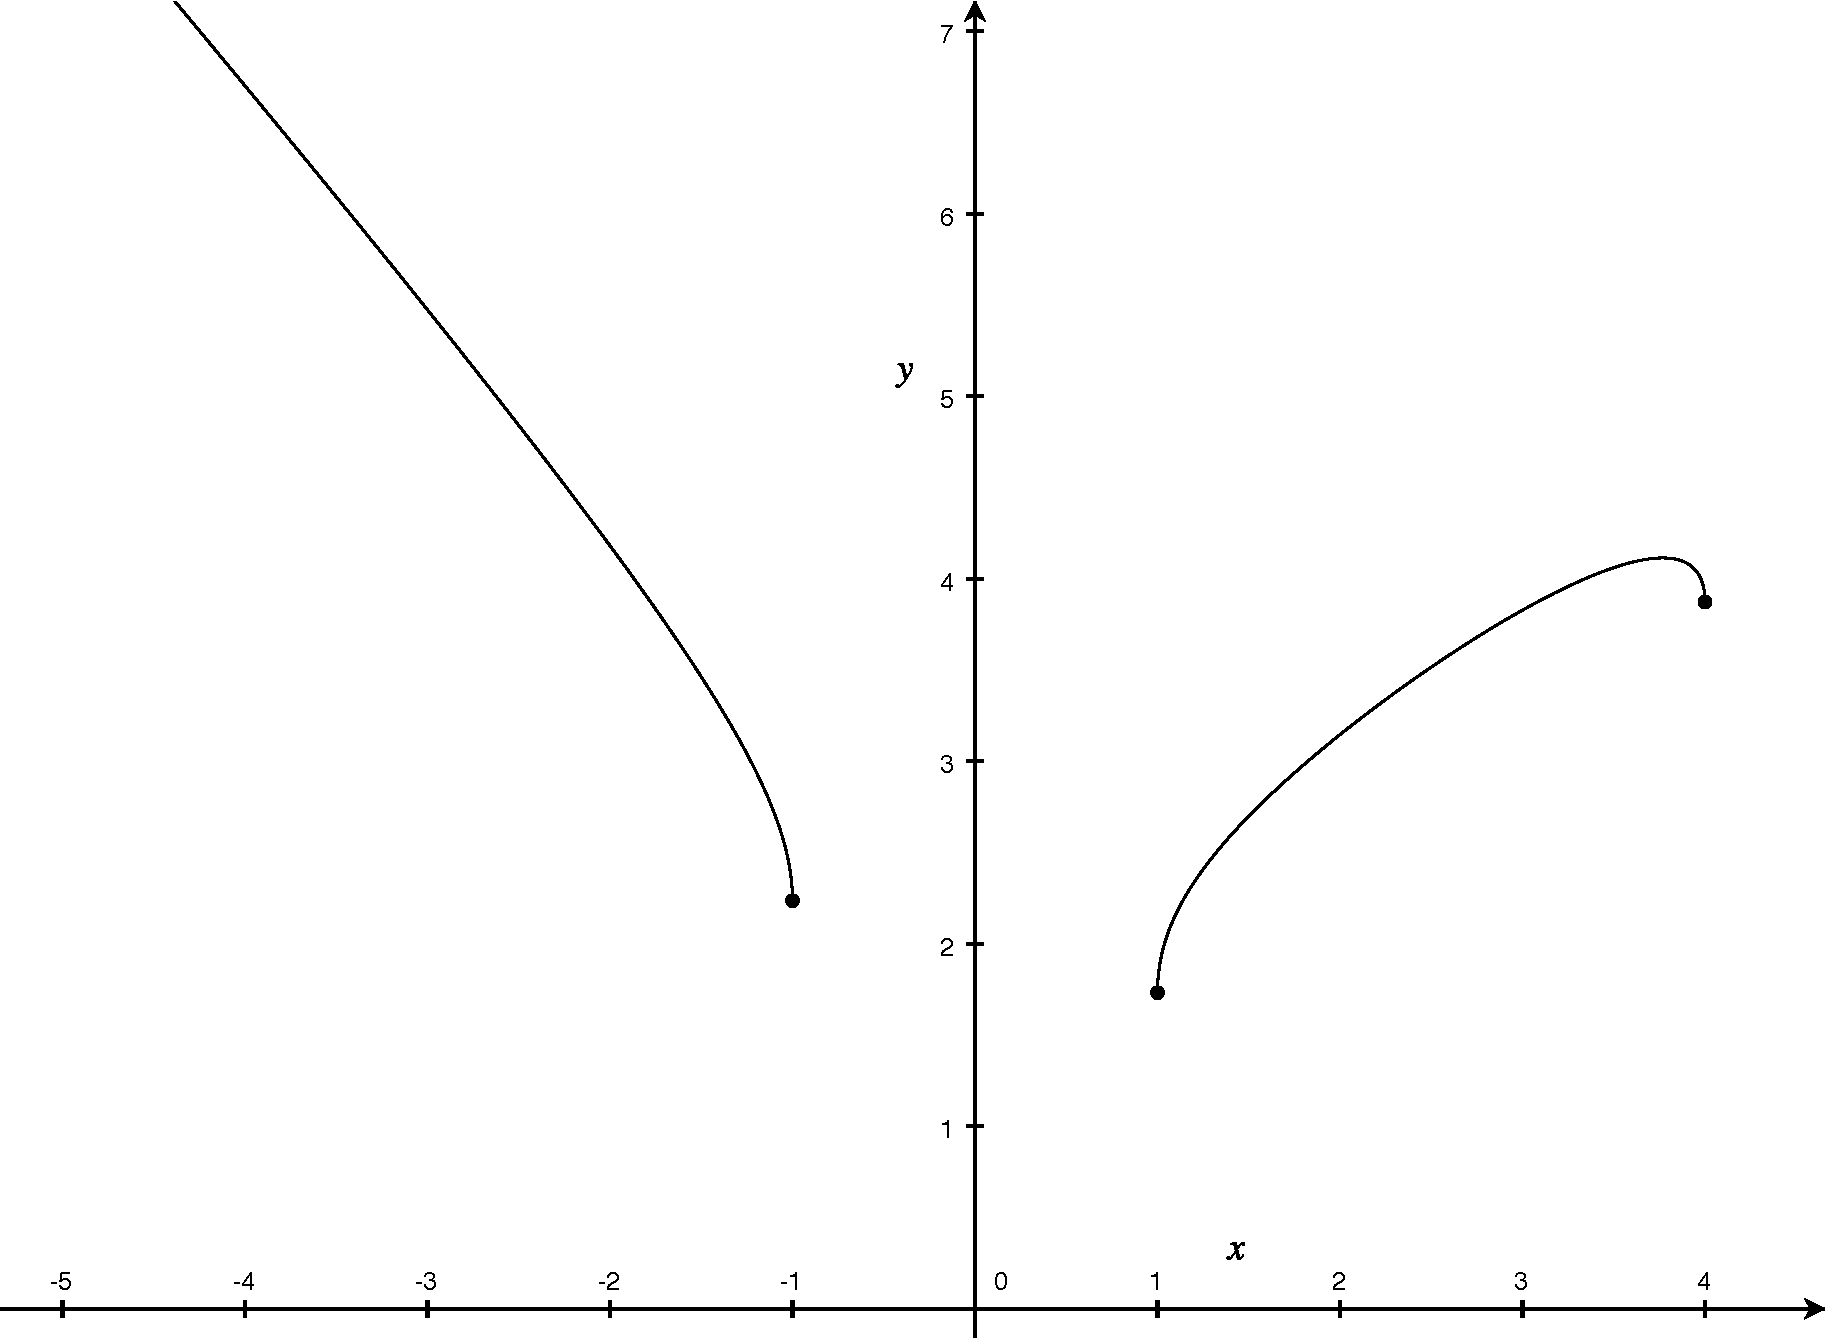
\includegraphics[width=.5\textwidth]{./graphics/graph10.pdf}
\caption{Partial graph of $h \left( x \right)$.}
\label{fig:graph10}
\end{figure}
% _-_-_-_-_-_-_-_-_-_-_-_-_-_-_-_-_-_-_-_-_-_-_-_-_-_-_-_-_-_-_-_-
\question Find the radius and center of the circle with equation $x^2+y^2-6x+10y+9=0$.
\begin{solution}
\begin{eqnarray*}
x^2+y^2-6x+10y+9&=&0\\
x^2-6x+y^2+10y&=&-9\\
x^2-6x+9+y^2+10y+25&=&-9+9+25\\
\left( x-3\right)^2 + \left( y+5\right)^2&=&5^2
\end{eqnarray*}
So the \fbox{center is $\left( 3, \ -5\right)$} and the \fbox{radius is $5$}.
\end{solution}
% _-_-_-_-_-_-_-_-_-_-_-_-_-_-_-_-_-_-_-_-_-_-_-_-_-_-_-_-_-_-_-_-
\question If $f \left( x \right) = x^3$, evaluate the difference quotient
\[
\frac{f \left( 2+h \right) - f \left( 2 \right)}{h}, \quad h \neq 0
\]
\begin{solution} Do I need to say it? Yes, the following is true if and only if $h \neq 0$.
\begin{eqnarray*}
\frac{f \left( 2+h \right) - f \left( 2 \right)}{h} &=& \frac{\left( 2+h \right)^3 - \left( 2 \right)^3}{h}\\
 &=& \frac{ 8+12h+6h^2+h^3- 8}{h}\\
  &=& \boxed{12+6h+h^2}
\end{eqnarray*}
\end{solution}
% _-_-_-_-_-_-_-_-_-_-_-_-_-_-_-_-_-_-_-_-_-_-_-_-_-_-_-_-_-_-_-_-
\question Solve for $x$.
\[
\frac{2x}{x+1} = \frac{2x-1}{x}
\]
\begin{solution}
\begin{eqnarray*}
\frac{2x}{x+1} &=& \frac{2x-1}{x}\\
2x \cdot x &=& \left( x+1\right) \left( 2x-1\right) \\
2x^2 &=& 2x^2 -x + 2x -1 \\
0&=& x -1 \\
1&=& x
\end{eqnarray*}
So, it appears that $\boxed{x=1}$ is a solution. Checking in the original equation, we have,
\[
\frac{2}{2} = \frac{1}{1},
\]
which is clearly true. 
\end{solution}
% _-_-_-_-_-_-_-_-_-_-_-_-_-_-_-_-_-_-_-_-_-_-_-_-_-_-_-_-_-_-_-_-
\question Verify the identity.
\[
\sin^2 \theta = \frac{\sec^2 \theta - 1}{\sec^2 \theta}
\]
\begin{solution}
Select the right side.
\begin{eqnarray*}
\frac{\sec^2 \theta - 1}{\sec^2 \theta} &=& \frac{\sec^2 \theta}{\sec^2 \theta} - \frac{1}{\sec^2 \theta}\\
&=& 1 - \cos^2 \theta\\
&=& \sin^2 \theta
\end{eqnarray*}
\emph{Q.E.D.}
\end{solution}
% _-_-_-_-_-_-_-_-_-_-_-_-_-_-_-_-_-_-_-_-_-_-_-_-_-_-_-_-_-_-_-_-
\question Solve for $x$.
\[
\frac{2x}{\sqrt{4-x}} -3\sqrt{4-x}= 0
\]
\begin{solution}
\begin{eqnarray*}
\frac{2x}{\sqrt{4-x}} -3\sqrt{4-x} &=& 0\\
\frac{2x}{\sqrt{4-x}}  &=& 3\sqrt{4-x}\\
2x &=& 3\left(4-x\right)\\
2x &=& 12-3x\\
5x &=& 12\\
x &=& \frac{12}{5}
\end{eqnarray*}
The solution (please check) is $\boxed{x=\frac{12}{5}}$.
\end{solution}
% _-_-_-_-_-_-_-_-_-_-_-_-_-_-_-_-_-_-_-_-_-_-_-_-_-_-_-_-_-_-_-_-
\question Find the domain of
\[
f\left(x \right) = \frac{x^2 - 49}{\sqrt{x^2 + 9} - 5}.
\]
\begin{solution} $x^2 + 9$ is always positive so we don't have to worry about the square root. However, to find the domain we need to solve $\sqrt{x^2 + 9} - 5 =0$.
\begin{eqnarray*}
\sqrt{x^2 + 9} - 5 &=& 0\\
\sqrt{x^2 + 9} &=& 5\\
x^2 + 9 &=& 25\\
x^2  &=& 16\\
x  &=& \pm 4
\end{eqnarray*}
So, the domain is $\boxed{\mathbb{R}, x \neq \pm 4}$.
\end{solution}
% _-_-_-_-_-_-_-_-_-_-_-_-_-_-_-_-_-_-_-_-_-_-_-_-_-_-_-_-_-_-_-_-
\question Solve the inequality.
\[
\left|  14 - x \right| - 3 < 17
\]
\begin{solution}
\begin{eqnarray*}
\left|  14 - x \right| - 3 &<& 17\\
\left|  14 - x \right|  &<& 20
\end{eqnarray*}
We know that for $a>0$, that $\left|  x  \right| < a$ is equivalent to $-a < x < a$, so
\begin{eqnarray*}
\left|  14 - x \right|  < 20\\
-20 <   14 - x   < 20\\
-34 <   - x   < 6\\
34 >   x   > -6\\
-6 <   x   < 34
\end{eqnarray*}
Here the proper interval is: $\boxed{\left(-6, \ 34 \right)}$.
\end{solution}
% _-_-_-_-_-_-_-_-_-_-_-_-_-_-_-_-_-_-_-_-_-_-_-_-_-_-_-_-_-_-_-_-
\question Solve by using an augmented matrix and elementary row operations.
\[
\left\{ {\begin{array}{rcrcrcr}
   2x   & + & 3y  & - & z & = &  -7\\
   3x   & - & 3y  & + & z & = &  12\\
   2x   & + & 4y  & + & z & = &  -3\\
\end{array}} \right.
\]
\begin{solution} Augmented matrix form of the system:
\[
\left[ {\begin{array}{rrr|r}
   2 &  3 &  -1 & -7 \\
   3 &  -3 &  1 &  12 \\
   2 &  4 &  1 & -3 \\
\end{array}} \right]
\]
Elementary row operations, in order given:
\begin{eqnarray*}
R_1 + R_2 \to R_2 \\
R_1 +   R_3 \to R_3 \\
\end{eqnarray*}
Produces:
\[
\left[ {\begin{array}{rrr|r}
   2 &  3 &  -1 & -7 \\
   3 &  -3 &  1 &  12 \\
   2 &  4 &  1 & -3 \\
\end{array}} \right]
\sim
\left[ {\begin{array}{rrr|r}
   2 &   3 &   -1 & -7 \\
   5 &  0 &  0 &  5 \\
   4 &   7 &   0 & -10 \\
\end{array}} \right]
\]
The second row gives $\boxed{x = 1}$; using $x = 1$ in row three, gives $\boxed{y=-2}$; finally, using $x = 1$ and $y=-2$ in row one, gives $\boxed{z=3}$.
\end{solution}
% _-_-_-_-_-_-_-_-_-_-_-_-_-_-_-_-_-_-_-_-_-_-_-_-_-_-_-_-_-_-_-_-
\question Use long division to find the quotient and remainder when $x^4 - 4x^2 + 2x +5$ is divided by $x-2$.
\begin{solution}
Doing the division gives a \fbox{remainder of 9} and a \fbox{quotient of $x^3+2x^2+2$}.
\end{solution}
% _-_-_-_-_-_-_-_-_-_-_-_-_-_-_-_-_-_-_-_-_-_-_-_-_-_-_-_-_-_-_-_-
\question Is $x=-1$ a root of the polynomial function $f\left( x \right) = 2x^3-5x^2-4x+3$?
\begin{solution}
\fbox{Yes}, because $f\left( -1 \right) = 0$.
\end{solution}
% _-_-_-_-_-_-_-_-_-_-_-_-_-_-_-_-_-_-_-_-_-_-_-_-_-_-_-_-_-_-_-_-
\question Factor\footnote{Previous problem may be helpful.} $f\left( x \right) = 2x^3-5x^2-4x+3$.
\begin{solution}
Using the fact that $x=-1$ is a root, we can divide $f\left( x \right)$ by $x+1$, getting
\[
\frac{2x^3-5x^2-4x+3}{x+1} = 2x^2-7x+3 = \left(2x - 1 \right) \left(x - 3 \right),
\]
so the complete factorization of $f\left( x \right)$ is
\[
\boxed{\left(x + 1 \right)\left(2x - 1 \right) \left(x - 3 \right)}.
\]
\end{solution}
\question Solve the inequality.
\[
\frac{3-2x}{x-1} + 2 \geq 0
\]
\begin{solution}
\begin{eqnarray*}
\frac{3-2x}{x-1} + 2 &\geq& 0\\
\frac{3-2x + 2 \left( x-1\right) }{x-1} &\geq& 0\\
\frac{3-2x + 2x-2 }{x-1} &\geq& 0\\
\frac{1 }{x-1} &\geq& 0
\end{eqnarray*}
Using simple sign analysis, the proper interval is: $\boxed{\left( 1, \ \infty \right)}$.
\end{solution}
% _-_-_-_-_-_-_-_-_-_-_-_-_-_-_-_-_-_-_-_-_-_-_-_-_-_-_-_-_-_-_-_-
\question Solve for $x$.
\[
\log_3 \left( 2x + 1 \right)  + \log_3 \left( 2x - 1 \right)  = 1
\]
\begin{solution}
\begin{eqnarray*}
\log_3 \left( 2x + 1 \right)  + \log_3 \left( 2x - 1 \right)  &=& 1\\
\log_3 \left( 2x + 1 \right)\left( 2x - 1 \right)  &=& 1\\
\log_3 \left( 4x^2 - 1 \right)  &=& 1\\
4x^2 - 1  &=& 3\\
4x^2 - 4  &=& 0\\
x^2 - 1  &=& 0\\
x &=& \pm 1
\end{eqnarray*}
The solutionis $\boxed{x=1}$ and you should check this.

\textbf{Note:} If you're limited to using real numbers only, whereas complex numbers can look mighty strange, such as the famous---or infamous---identity $e^{i\pi} + 1 =0$.
\end{solution}

% _-_-_-_-_-_-_-_-_-_-_-_-_-_-_-_-_-_-_-_-_-_-_-_-_-_-_-_-_-_-_-_-
\question Given
\[
f\left( x \right) = \frac{2x-1}{2-3x},
\]
find and simplify the difference quotient
\[
\frac{f\left( x + h\right) - f\left( x \right)}{h}, \quad h \neq 0.
\]
\begin{solution}
Do I need to say it? Yes, the following is true if and only if $h \neq 0$.
\begin{eqnarray*}
\frac{f\left( x + h\right) - f\left( x \right)}{h} &=& \frac{\ \displaystyle \frac{2x + 2h -1}{2 - 3x - 3h} + \frac{2x-1}{2-3x} \ }{h}\\
&=& \frac{\ \left(2x + 2h -1\right)\left(2-3x\right) - \left(2x-1\right)\left(2 - 3x - 3h\right) \ }{h\left(2 - 3x - 3h\right)\left(2-3x\right)}\\
&=& \frac{\ 4x + 4h -2  -6x^2 -6xh +3x  -4x+2 + 6x^2-3x   +6xh-3h \ }{h\left(2 - 3x - 3h\right)\left(2-3x\right)}\\
&=& \frac{\  h \ }{h\left(2 - 3x - 3h\right)\left(2-3x\right)}\\
&=& \boxed{\frac{\  1 \ }{\left(2 - 3x - 3h\right)\left(2-3x\right)}}\\
\end{eqnarray*}
\end{solution}
% _-_-_-_-_-_-_-_-_-_-_-_-_-_-_-_-_-_-_-_-_-_-_-_-_-_-_-_-_-_-_-_-
\question Find the domain of
\[
f\left(x \right) = \frac{x + 2}{\sqrt{2x^2 - 18}}.
\]
\begin{solution}
Finding the domain requires solving $2x^2 - 18 > 0$ for $x$.
\begin{eqnarray*}
2x^2 - 18 &>& 0\\
x^2 - 9 &>& 0\\
\left( x - 3 \right) \left( x + 3 \right) &>& 0
\end{eqnarray*}
Simple sign analysis gives $\boxed{\left( -\infty, \ -3 \right) \cup \left( 3, \ \infty \right)}$.
\end{solution}
\question Given
\[
f \left( x \right) = \left( x + 3 \right)^2, \quad x \geq -3,
\]
find $f^{-1} \left( x \right)$. Graphing may be helpful, but is not required.
\begin{solution}
The domain of $f \left( x \right)$ is $\left[-3, \infty \right)$ and the range is $\left[0, \infty \right)$, so the domain of $f^{-1} \left( x \right)$ is $\left[0, \infty \right)$ and the range is  $\left[-3, \infty \right)$.
\begin{eqnarray*}
f \left( x \right) &=& \left( x + 3 \right)^2\\
y &=& \left( x + 3 \right)^2\\
x &=& \left( y + 3 \right)^2\\
\pm \sqrt{x} &=& y + 3\\
\pm \sqrt{x} -3 &=& y
\end{eqnarray*}
However, since $y \geq -3$ we have
\[
\boxed{f^{-1} \left( x \right) = \sqrt{x} -3, \quad x \geq 0}.
\]
\end{solution}
\question Given
\[
f \left( x \right) =\sqrt{x+6} \quad {\rm{and}} \quad g \left( x \right) =x^2 - 5,
\]
answer each of the following questions.
\begin{parts}
\part Find $\left( f \circ g \right) \left( x \right)$
\begin{solution}
\[
\left( f \circ g \right) \left( x \right) = f \left( g \left( x \right) \right) = f \left( x^2 - 5 \right) = \sqrt{x^2 - 5 +6}= \boxed{\sqrt{x^2 +1}}
\]
\end{solution}
\part The domain of $\left( f \circ g \right) \left( x \right)$
\begin{solution}
$\boxed{\mathbb{R}}$.
\end{solution}
\part Find $\left( g \circ f \right) \left( x \right)$
\begin{solution} 
\[
\left( g \circ f \right) \left( x \right) = g \left( f \left( x \right)\right) = g \left( \sqrt{x+6}\right) = \left(\sqrt{x+6}\right)^2 - 5 = x+6-5=\boxed{x+1}
\]
\end{solution}
\part The domain of $\left( g \circ f \right) \left( x \right)$
\begin{solution}
$\boxed{x \geq -6}$.
\end{solution}
\end{parts}
\question Given
\[
f \left( x \right) = 2x^4 + 7x^3 - 4x^2 - 27x - 18, \quad {\rm{and}} \quad f \left( 2 \right) = f \left( -3 \right) = 0
\]
answer the following questions.
\begin{parts}
\part Use the given roots, and long division, to completely factor $f \left( x \right)$.
\begin{solution}
Since we are given two roots, we know two factors of $f \left( x \right)$ are $\left( x-2\right)$ and $\left( x+3\right)$. Dividing $f \left( x \right)$ by the product of these two factors gives
\[
2x^2 + 5x + 3 = \left( 2x+3\right)\left( x+1\right).
\]
So the complete factorization of $f \left( x \right)$ is
\[
\boxed{\left( 2x+3\right)\left( x+1\right)\left( x-2\right)\left( x+3\right)}
\]
\end{solution}
\part Graph $f \left( x \right)$ using the roots, $y$-intercept and sign-analyses.
\begin{solution}
Your graph (Figure \ref{fig:graph20}, page \pageref{fig:graph20}) does not need to have such precise detail as mine, but it should still reflect the key pre-calculus analysis.
\end{solution}
\begin{figure}[hbtp]
\centering
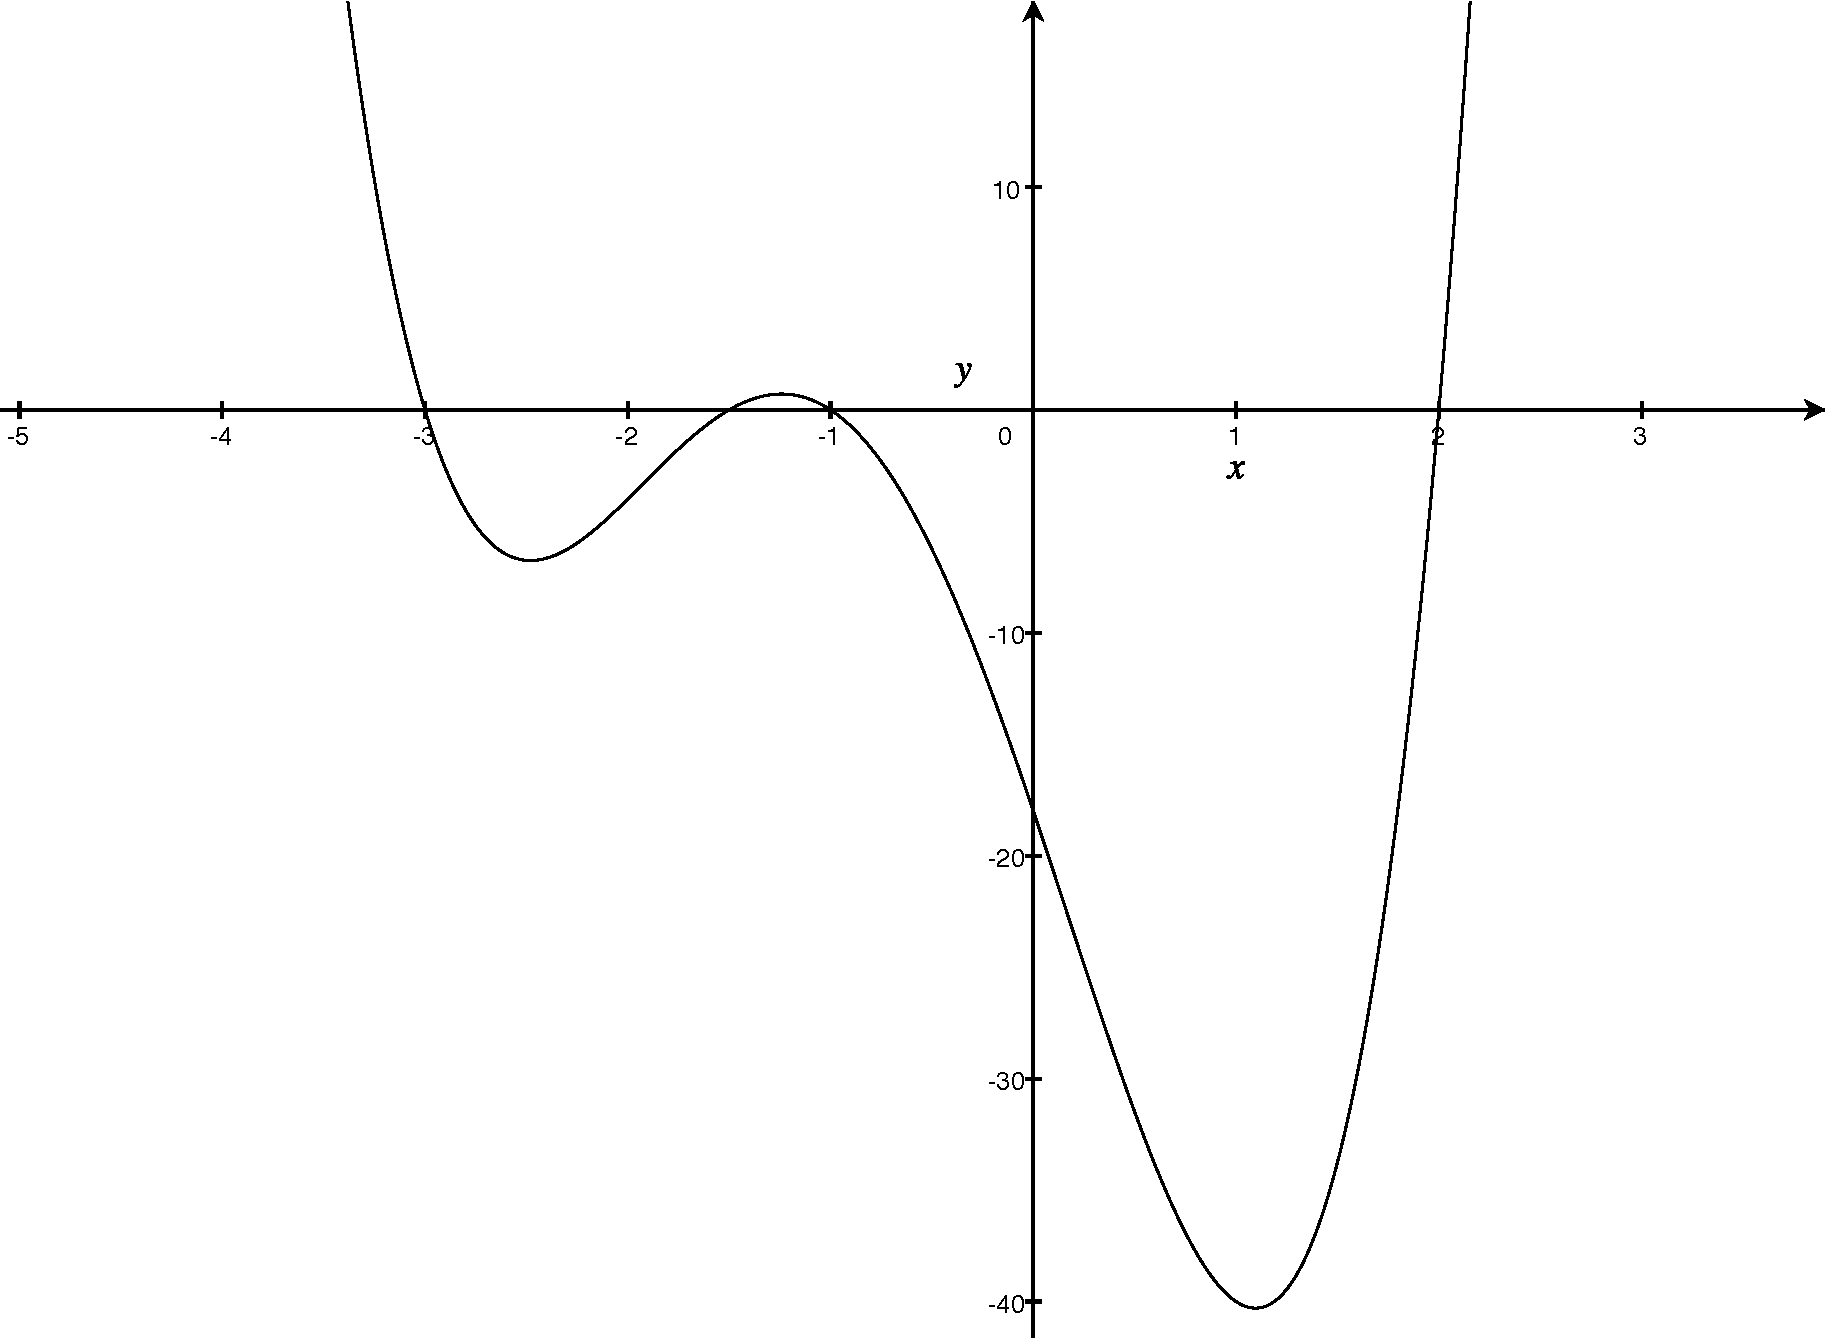
\includegraphics[width=.5\textwidth]{./graphics/graph20.pdf}
\caption{Graph of $f \left( x \right)$.}
\label{fig:graph20}
\end{figure}
\end{parts}
\question Given
\[
f \left( x \right) = \frac{x^3 + 2 x^2}{x^2 + 1},
\]
answer the following questions.
\begin{parts}
\part $x$-intercept(s) in point form.
\begin{solution} Set $f \left( x \right) = 0$ and solve for $x$.
\begin{eqnarray*}
0 &=& \frac{x^3 + 2 x^2}{x^2 + 1}\\
0 &=& \frac{x^2 \left(x + 2\right)}{x^2 + 1}
\end{eqnarray*}
Clearly, \fbox{$\left( -2, \ 0 \right)$ and $\left( 0, \ 0 \right)$}.
\end{solution}
\part $y$-intercept in point form.
\begin{solution}
Set $x=0$ and evaluate.  Clearly, \fbox{$\left( 0, \ 0 \right)$}.
\end{solution}
\part All linear asymptotes in equation form.
\begin{solution}
Since the degree of the numerator is one more than the denominator, we have the possibility of getting a slant asymptote. The long division gives
\[
f \left( x \right) = \frac{x^3 + 2 x^2}{x^2 + 1} = x + 2 -  \frac{x+2}{x^2 + 1},
\]
so the slant asymptote is $\boxed{y = x + 2}$.
\end{solution}
\part Graph $f \left( x \right)$ using the information above and sign-analyses.
\begin{solution}
Your graph (Figure \ref{fig:graph30}, page \pageref{fig:graph30})  does not need to have such precise detail as mine, but it should still reflect the key pre-calculus analysis.
\end{solution}
\begin{figure}[hbtp]
\centering
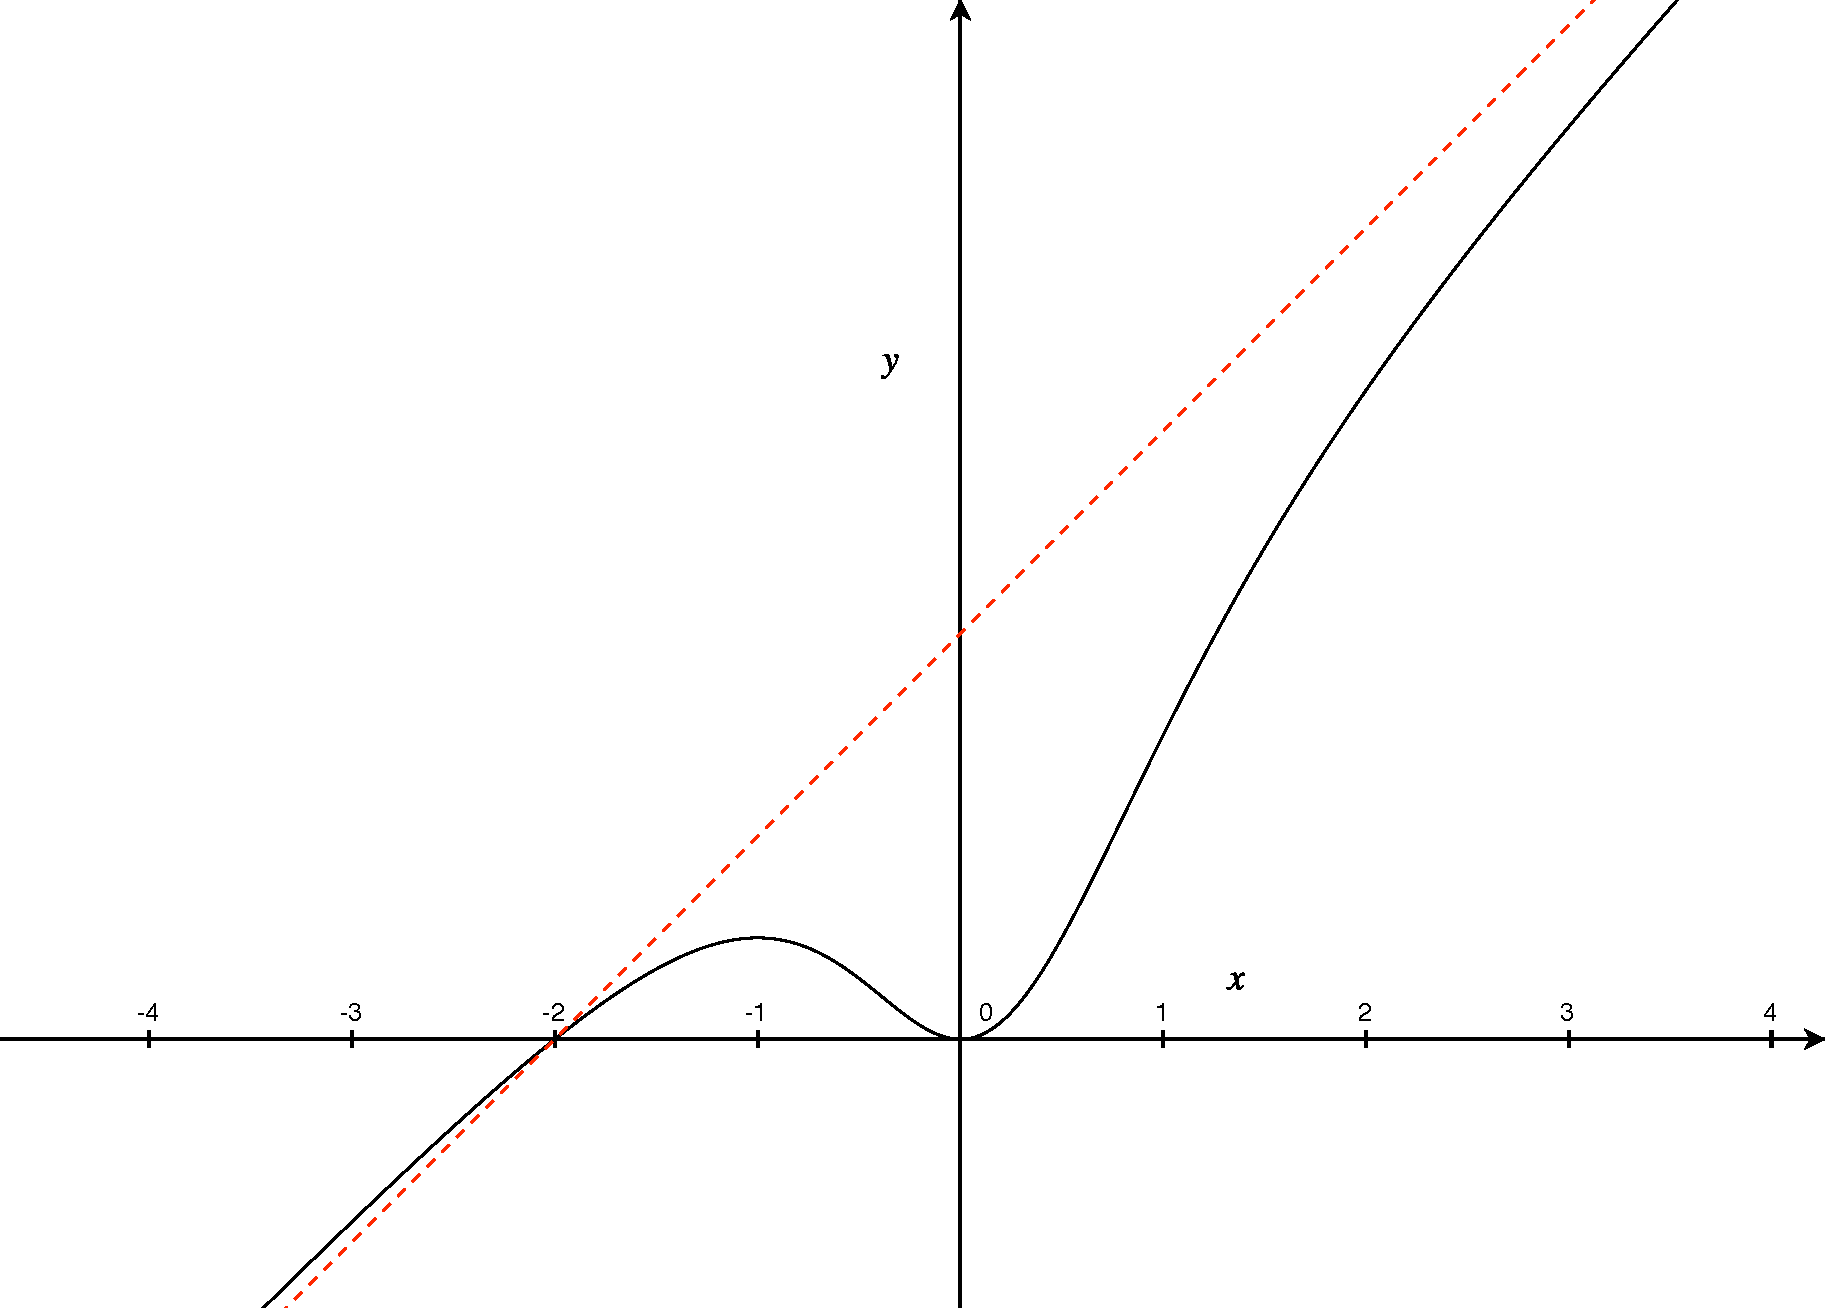
\includegraphics[width=.5\textwidth]{./graphics/graph30.pdf}
\caption{Graph of $f \left( x \right)$.}
\label{fig:graph30}
\end{figure}
\end{parts}
% _-_-_-_-_-_-_-_-_-_-_-_-_-_-_-_-_-_-_-_-_-_-_-_-_-_-_-_-_-_-_-_-
\question Given
\[
f\left( x \right) = x^2 - x + 1,
\]
find and simplify the difference quotient
\[
\frac{f\left( x + h\right) - f\left( x \right)}{h}, \quad h \neq 0.
\]
\begin{solution}
Do I need to say it? Yes, the following is true if and only if $h \neq 0$.
\begin{eqnarray*}
\frac{f\left( x + h\right) - f\left( x \right)}{h} &=& \frac{\left( x + h\right)^2 - \left( x + h\right) + 1 - \left( x^2 - x + 1\right)}{h}\\
&=& \frac{x^2 + 2xh + h^2 - x - h + 1 -  x^2 + x - 1}{h}\\
&=& \frac{ 2xh + h^2 - h}{h}\\
&=& \boxed{2x + h - 1}
\end{eqnarray*}
\end{solution}
% _-_-_-_-_-_-_-_-_-_-_-_-_-_-_-_-_-_-_-_-_-_-_-_-_-_-_-_-_-_-_-_-
\question Solve the inequality.
\[
\left|  14-3x  \right| -5 > -2
\]
\begin{solution}
\begin{eqnarray*}
\left|  14-3x  \right| -5 &>& -2\\
\left|  14-3x  \right|  &>& 3\\
\end{eqnarray*}
We know that $\left|  x  \right| > a$ is equivalent to $x > a$ or $x< -a$, so
\begin{eqnarray*}
\left|  14-3x  \right|  > 3 \quad \Rightarrow  \quad 14-3x > 3 \quad &\mbox{or}& \quad 14-3x < -3\\
x < 11/3 \quad &\mbox{or}& \quad 17/3  < x
\end{eqnarray*}
Here the proper intervals are: $\boxed{\left(-\infty, \ 11/3 \right) \cup \left( 17/3, \ \infty \right)}$.
\end{solution}
% _-_-_-_-_-_-_-_-_-_-_-_-_-_-_-_-_-_-_-_-_-_-_-_-_-_-_-_-_-_-_-_-
\question Write the system of linear equations represented by the augmented matrix. Then use back-substitution to find the solution. (Use the variables $x$, $y$, and $z$.)
\[
\left[ {\begin{array}{rrr|r}
   {1} & {-1} & {2} & {4} \\
   {0} & {1} & {-1}  & {2}\\
{0} & {0} & {1}  & {-2}
\end{array}} \right]
\]
\begin{solution}
\[
\left\{ {\begin{array}{*{20}c}
   {x} &  -  & {y} &  +  & {2z} &  =  & 4  \\
   {} &    & {y} &  -  & {z} &  =  & 2  \\
   {} &    & {} &    & {z} &  =  & -2  \\
\end{array}} \right.
\]
The last line gives $\boxed{z = -2}$, then using the value for $z$ in line two, we get $\boxed{y = 0}$, finally using these two values in line one we get $\boxed{x = 8}$.
\end{solution}
% _-_-_-_-_-_-_-_-_-_-_-_-_-_-_-_-_-_-_-_-_-_-_-_-_-_-_-_-_-_-_-_-
\question Condense the expression to the logarithm of a single quantity.
\[
\frac{1}{3} \left[ 2 \ln \left( x+3 \right) + \ln x - \ln \left( x^2 - 1\right) \right]
\]
\begin{solution}
\begin{eqnarray*}
\frac{1}{3} \left[ 2 \ln \left( x+3 \right) + \ln x - \ln \left( x^2 - 1\right) \right] &=& \frac{1}{3} \left[  \ln \left( x+3 \right)^2 + \ln x - \ln \left( x^2 - 1\right) \right]\\
&=& \frac{1}{3} \left[  \ln \frac{x\left( x+3 \right)^2}{x^2 - 1} \right]\\
&=& \boxed{\ln \sqrt[3]{\frac{x\left( x+3 \right)^2}{x^2 - 1}}}
\end{eqnarray*}
\end{solution}
% _-_-_-_-_-_-_-_-_-_-_-_-_-_-_-_-_-_-_-_-_-_-_-_-_-_-_-_-_-_-_-_-
\question Solve for $x$.
\[
\left( \frac{2}{3} \right)^x = \frac{81}{16}
\]
\begin{solution}
\begin{eqnarray*}
\left( \frac{2}{3} \right)^x &=& \frac{81}{16}\\
\left( \frac{2}{3} \right)^x &=& \left(\frac{3}{2}\right)^4\\
\left( \frac{2}{3} \right)^x &=& \left(\frac{2}{3}\right)^{-4}\\
\end{eqnarray*}
So, $\boxed{x = -4}$.
\end{solution}
% _-_-_-_-_-_-_-_-_-_-_-_-_-_-_-_-_-_-_-_-_-_-_-_-_-_-_-_-_-_-_-_-
\question Solve the inequality.
\[
\frac{x+6}{x+1} - 2 < 0
\]
\begin{solution}
\begin{eqnarray*}
\frac{x+6}{x+1} - 2 &<& 0\\
\frac{x+6}{x+1} - \frac{2\left(x+1\right)}{x+1} &<& 0\\
\frac{4-x}{x+1} &<& 0\\
\end{eqnarray*}
Using simple sign analysis, the proper intervals are: $\boxed{\left(-\infty, \ -1 \right) \cup \left( 4, \ \infty \right)}$.
\end{solution}
% _-_-_-_-_-_-_-_-_-_-_-_-_-_-_-_-_-_-_-_-_-_-_-_-_-_-_-_-_-_-_-_-
\question Solve algebraically (exact answer) and then approximate to three decimal places.
\[
-2 + 2 \ln 3x = 17
\]
\begin{solution}
\begin{eqnarray*}
-2 + 2 \ln 3x &=& 17\\
 2 \ln 3x &=& 19\\
\ln 3x &=& \frac{19}{2}\\
 3x &=& e^{19/2}\\
 x &=& \boxed{\frac{e^{19/2}}{3} \approx 4,453.242}
\end{eqnarray*}
\end{solution}
% _-_-_-_-_-_-_-_-_-_-_-_-_-_-_-_-_-_-_-_-_-_-_-_-_-_-_-_-_-_-_-_-
\question Given
\[
f \left( x \right) = \frac{x^2-3x+2}{2x^2+5x+3} = \frac{\left(x-1\right)\left(x-2\right)}{\left(2x+3\right)\left(x+1\right)},
\]
answer the following questions:
\begin{parts}
\part $x$-intercepts in point form.
\begin{solution}
$\boxed{\left(1, \ 0 \right); \left(2, \ 0 \right)}$
\end{solution}
\part $y$-intercept in point form.
\begin{solution}
$\boxed{\left(0, \ 2/3 \right)}$
\end{solution}
\part Equation of the horizontal asymptote.
\begin{solution}
$\boxed{y = 1/2}$
\end{solution}
\part Equation of the vertical asymptotes.
\begin{solution}
$\boxed{x = -1; x = -3/2}$
\end{solution}
\part Graph $f\left( x \right)$ using the above information and sign analysis.
\begin{solution}
Your graph (Figure \ref{fig:graph40}, page \pageref{fig:graph40})  should roughy look like the one below.
\end{solution}
\begin{figure}[htbp]
   \centering
   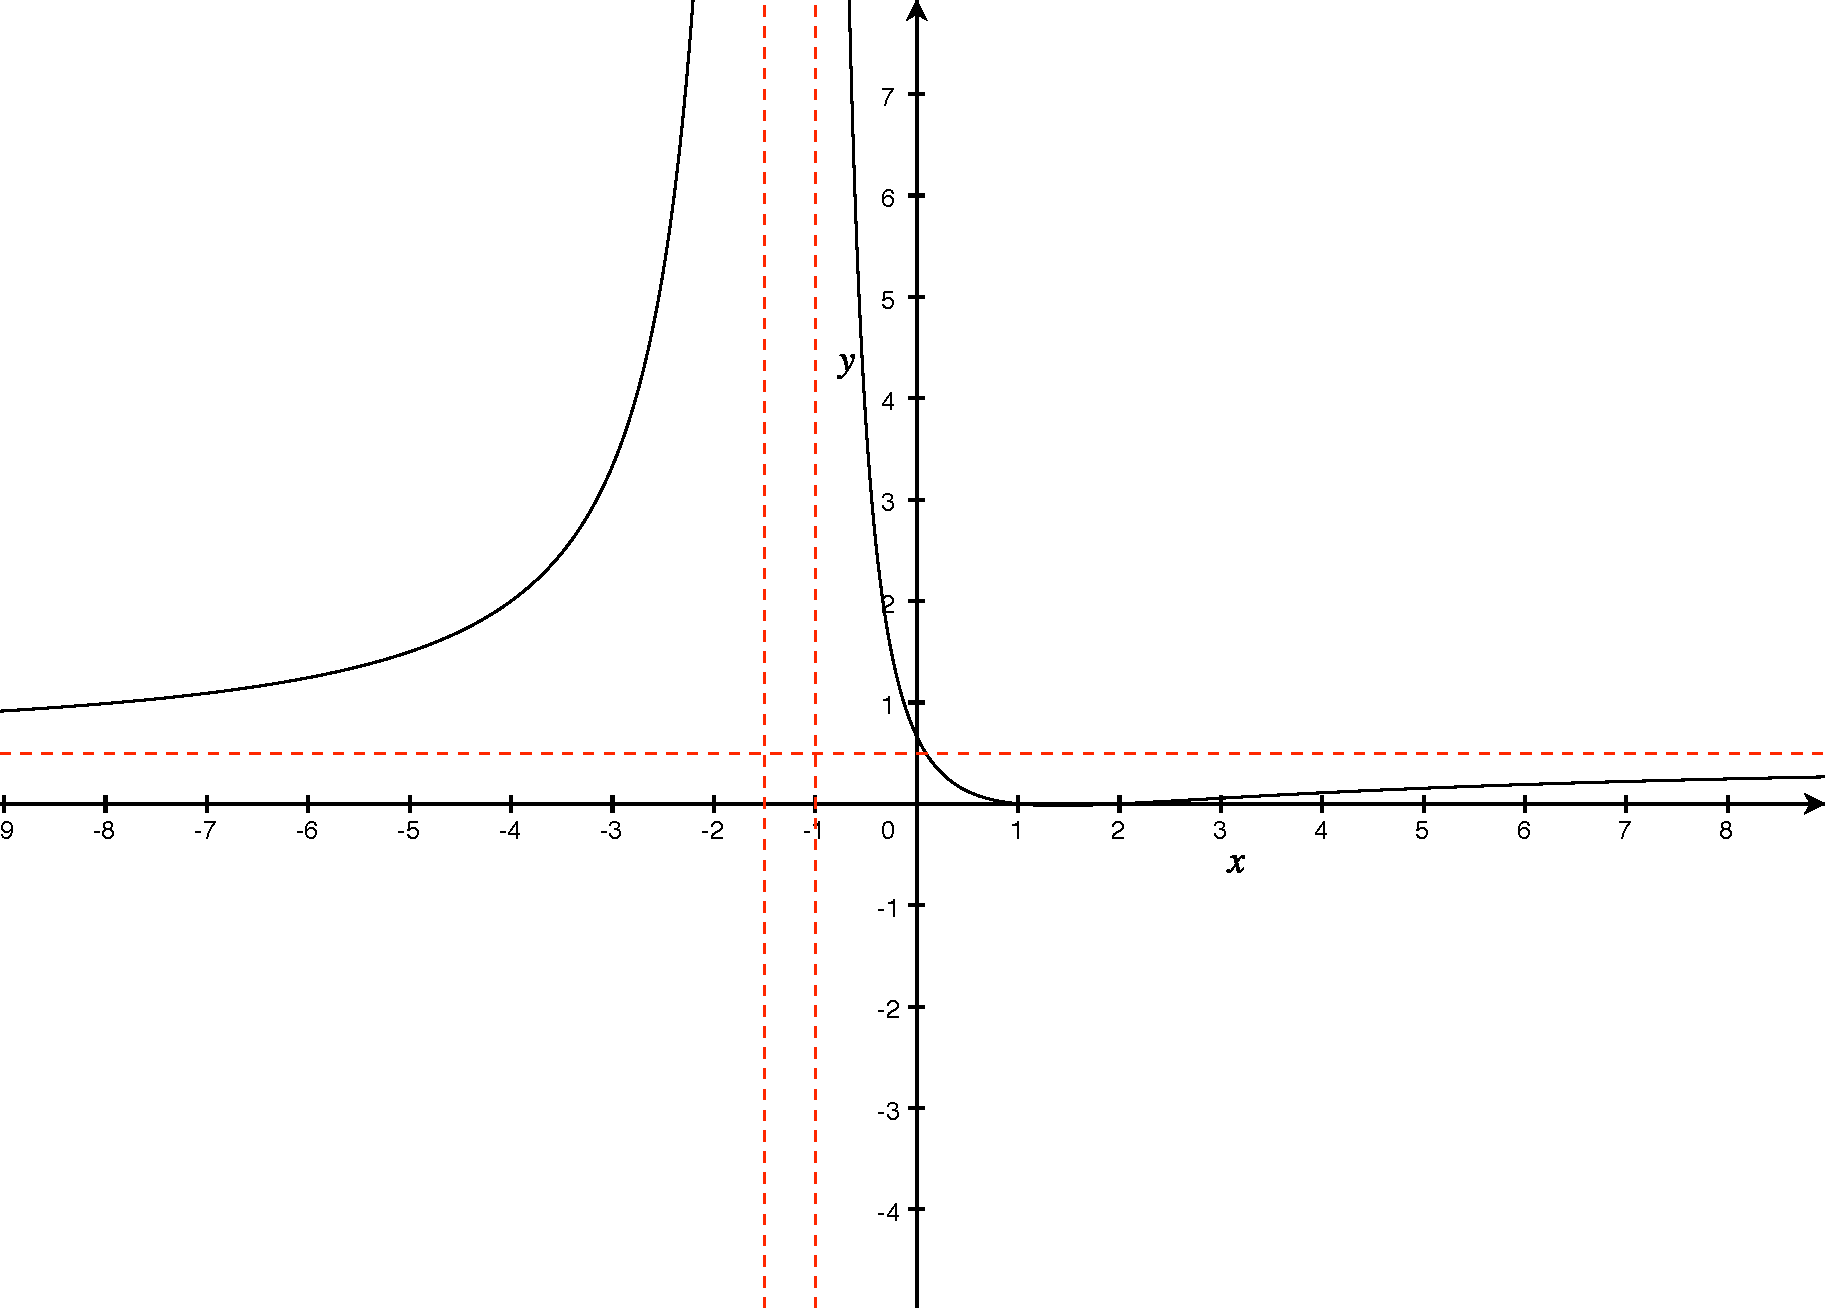
\includegraphics[width=.5\textwidth]{./graphics/graph40.pdf} 
   \caption{Graph of $f \left( x \right)$.}
   \label{fig:graph40}
\end{figure}
\end{parts}
% _-_-_-_-_-_-_-_-_-_-_-_-_-_-_-_-_-_-_-_-_-_-_-_-_-_-_-_-_-_-_-_-
\question Use summation notation to write the given sum.
\[
3+9+27+81+\cdots+729
\]
\begin{solution} Here's one possible answer.
\[
3+9+27+81+\cdots+729 = \boxed{\sum\limits_{n = 1}^{6} 3^n}
\]
\end{solution}
% _-_-_-_-_-_-_-_-_-_-_-_-_-_-_-_-_-_-_-_-_-_-_-_-_-_-_-_-_-_-_-_-
\question Find the rational number representation of the given repeating decimal.
\[
 1.2\overline{87}
\]
\begin{solution} Let $x = 1.2\overline{87}$.
\begin{eqnarray*}
10x &=& 12.\overline{87}\\
1000x &=& 1287.\overline{87}\\
1000x-10x &=& 1287.\overline{87} - 12.\overline{87}\\
990x &=& 1275.00\overline{00}\\
x &=& \boxed{\frac{1275}{990}} = \boxed{\frac{85}{66}}
\end{eqnarray*}
\end{solution}
% _-_-_-_-_-_-_-_-_-_-_-_-_-_-_-_-_-_-_-_-_-_-_-_-_-_-_-_-_-_-_-_-
\question Use your calculator to approximate each of the following to three decimal places.
\begin{parts}
\part $\arcsin{\left(-0.987\right)}$
\begin{solution}
$\arcsin{\left(-0.987\right)} \approx \boxed{-1.409 \quad {\rm{or}} \quad -80.751^\circ}$
\end{solution}
\part $\arctan{\left(-89.456\right)}$
\begin{solution}
$\arctan{\left(-89.456\right)} \approx \boxed{-1.560 \quad {\rm{or}} \quad -89.360^\circ}$
\end{solution}
\part $\arccos{\left(-0.009\right)}$
\begin{solution}
$\arccos{\left(-0.009\right)} \approx \boxed{1.580 \quad {\rm{or}} \quad 90.516^\circ}$
\end{solution}
\end{parts}
\question Find the exact value of the following.
\begin{parts}
\part $\arccos{\left(\displaystyle \frac{1}{\sqrt{2}}\right)}$
\begin{solution}
$\arccos{\left(\displaystyle \frac{1}{\sqrt{2}}\right)} = \boxed{\frac{\pi}{4} \quad {\rm{or}} \quad 45^\circ}$
\end{solution}
\part $\arccos{\left[\sin\left(\displaystyle \frac{5\pi}{3}\right)\right]}$
\begin{solution}
$\arccos{\left[\sin\left(\displaystyle \frac{5\pi}{3}\right)\right]} = \arccos{\left(\displaystyle -\frac{\sqrt{3}}{2}\right)} = \boxed{\frac{5\pi}{6} \quad {\rm{or}} \quad 150^\circ}$
\end{solution}
\end{parts}
% _-_-_-_-_-_-_-_-_-_-_-_-_-_-_-_-_-_-_-_-_-_-_-_-_-_-_-_-_-_-_-_-
\question Simplify the factorial expression.
\[
\frac{\left(2n + 2 \right)!}{\left( 2n\right)!}
\]
\begin{solution}
\[
\frac{\left(2n + 2 \right)!}{\left( 2n\right)!} = \frac{\left(2n + 2 \right) \left(2n + 1 \right) \left(2n\right)!}{\left( 2n\right)!} = \boxed{\left(2n + 2 \right) \left(2n + 1 \right) = 4n^2 + 6n + 2}
\]
\end{solution}
% _-_-_-_-_-_-_-_-_-_-_-_-_-_-_-_-_-_-_-_-_-_-_-_-_-_-_-_-_-_-_-_-
\question A ramp 21 feet in length rises to a loading platform that is 5 feet off the ground. Assuming that the ground is level, what is the angle (to the nearest whole degree) between the ramp and the ground?
\begin{solution} You should draw a diagram first.
\[
\sin \theta = \frac{5}{21}, \quad \Rightarrow \quad \arcsin \left( \frac{5}{21} \right) \approx \boxed{14^\circ}
\]
\end{solution}
% _-_-_-_-_-_-_-_-_-_-_-_-_-_-_-_-_-_-_-_-_-_-_-_-_-_-_-_-_-_-_-_-
\question Write an algebraic expression that is equivalent to
\[
\sec \left[ \arcsin \left( x - 1 \right) \right].
\]
\begin{solution} You should draw a triangle first and use the Pythagorean Theorem to determine the missing side.
\[
\sec \left[ \arcsin \left( x - 1 \right) \right] = \boxed{\frac{1}{\sqrt{2x-x^2}}}
\]
\end{solution}
% _-_-_-_-_-_-_-_-_-_-_-_-_-_-_-_-_-_-_-_-_-_-_-_-_-_-_-_-_-_-_-_-
\question Find the \emph{numerical coefficient} of the term whose variable part is $x^6y^3$ in the expansion of $\left( x - 2y \right)^9$.
\begin{solution}
\[
\left( {\begin{array}{c}
   9  \\
   6
\end{array} } \right) \left(x \right)^6 \left( -2y\right)^3 = 84 \cdot \left( -8\right) x^6y^3 = -672 x^6y^3
\]
So, the numerical coefficient is \fbox{$-672$}.
\end{solution}
% _-_-_-_-_-_-_-_-_-_-_-_-_-_-_-_-_-_-_-_-_-_-_-_-_-_-_-_-_-_-_-_-
\question Solve for $x$.
\begin{parts}
\part $\sin x + \sqrt{2} = - \sin x$ in the interval $\left[ 0, \ 2 \pi\right)$.
\begin{solution} 
\begin{eqnarray*}
\sin x + \sqrt{2} &=& - \sin x\\
2\sin x  &=& - \sqrt{2}\\
\sin x  &=& - \frac{\sqrt{2}}{2}.
\end{eqnarray*}
The reference is $45^\circ$ and the solutions occur in the third and fourth quadrant, so
\[
x = 45^\circ + 180^\circ = 225^\circ =\boxed{\frac{5\pi}{4}} \qquad {\rm{and}} \qquad x =  360^\circ - 45^\circ= 315^\circ = \boxed{\frac{7\pi}{4}}
\]
\end{solution}
\part $2 \sin^2 x - \sin x - 1 = 0$ in the interval $\left[ 0, \ 2 \pi\right)$.
\begin{solution} 
\begin{eqnarray*}
2 \sin^2 x - \sin x - 1 &=& 0\\
\left( 2 \sin x + 1 \right) \left( \sin x - 1 \right) &=& 0.
\end{eqnarray*}
Which gives two equations to solve.
\[
\sin x = -\frac{1}{2} \qquad {\rm{and}} \qquad \sin x = 1.
\]
The reference for the first equation is $30^\circ$ and the solutions occur in the third and fourth quadrant, so
\[
x = 30^\circ + 180^\circ = 210^\circ =\boxed{\frac{7\pi}{6}} \qquad {\rm{and}} \qquad x =  360^\circ - 30^\circ= 330^\circ = \boxed{\frac{11\pi}{6}},
\]
and the solution to the second equation is \fbox{$x = \displaystyle \frac{\pi}{2}$}
\end{solution}
\end{parts}
% _-_-_-_-_-_-_-_-_-_-_-_-_-_-_-_-_-_-_-_-_-_-_-_-_-_-_-_-_-_-_-_-
\question Write an expression for the $n^{\rm{th}}$ term.\footnote{Let $n$ start at $1$, that is $a_1 = 1$.}
\[
1, \ \frac{5}{2}, \frac{25}{6}, \ \frac{125}{24}, \ \frac{625}{120}, \ldots
\]
\begin{solution}
\[
\boxed{a_n = \frac{5^{n-1}}{n!}}
\]
\end{solution}
% _-_-_-_-_-_-_-_-_-_-_-_-_-_-_-_-_-_-_-_-_-_-_-_-_-_-_-_-_-_-_-_-
\question Convert each of the following angle measures to radian measure.
\begin{parts}
\part $60^\circ$
\begin{solution}
\[
60^\circ = 60^\circ \cdot \left( \frac{\pi}{180^\circ} \right) = \boxed{\frac{\pi}{3}}
\]
\end{solution}
\part $90^\circ$
\begin{solution}
\[
90^\circ = 90^\circ \cdot \left( \frac{\pi}{180^\circ} \right) = \boxed{\frac{\pi}{2}}
\]
\end{solution}
\part $50^\circ$
\begin{solution}
\[
50^\circ = 50^\circ \cdot \left( \frac{\pi}{180^\circ} \right) = \boxed{\frac{5\pi}{18}}
\]
\end{solution}
\end{parts}
% _-_-_-_-_-_-_-_-_-_-_-_-_-_-_-_-_-_-_-_-_-_-_-_-_-_-_-_-_-_-_-_-
\question Use the Binomial Theorem to expand and simplify
\[
\left( 3\sqrt[3]{x^2} - 2\sqrt[3]{y}\right)^3.
\]
\begin{solution} First the expansion
\[
\boxed{\left( 3\sqrt[3]{x^2} \right)^3
+
3 \left( 3\sqrt[3]{x^2} \right)^2\left( - 2\sqrt[3]{y} \right)
+
3 \left( 3\sqrt[3]{x^2} \right)\left( - 2\sqrt[3]{y} \right)^2
+
 \left( - 2\sqrt[3]{y} \right)^3},
\]
then the simplification
\[
\boxed{ 27x^2 - 54 \sqrt[3]{x^4y} + 36 \sqrt[3]{x^2y^2} - 8y}.
\]
\end{solution}

% _-_-_-_-_-_-_-_-_-_-_-_-_-_-_-_-_-_-_-_-_-_-_-_-_-_-_-_-_-_-_-_-

\question Evaluate (exact values) all six trigonometric functions for $x = -120^\circ$.
\begin{parts}
\part $\sin x$
\begin{solution}
$\sin x = \boxed{ - \frac{\sqrt{3}}{2}}$
\end{solution}
\part $\cos x$
\begin{solution}
$\cos x = \boxed{ - \frac{1}{2}}$
\end{solution}
\part $\tan x$
\begin{solution}
$\tan x = \boxed{ \sqrt{3}}$
\end{solution}
\part $\cot x$
\begin{solution}
$\cot x = \boxed{ \frac{1}{\sqrt{3}}}$
\end{solution}
\part $\sec x$
\begin{solution} 
$\sec x = \boxed{ - 2}$
\end{solution}
\part $\csc x$
\begin{solution} 
$\csc x = \boxed{ - \frac{2}{\sqrt{3}}}$
\end{solution}
\end{parts}
% _-_-_-_-_-_-_-_-_-_-_-_-_-_-_-_-_-_-_-_-_-_-_-_-_-_-_-_-_-_-_-_-
\question Find the sum.
\[
\sum\limits_{n = 48}^{70} \left( 2n - 1 \right)
\]
\begin{solution} Expand first. You should also notice that there are $70-48+1=23$ terms.
\begin{eqnarray*}
\sum\limits_{n = 48}^{70} \left( 2n - 1 \right) &=& \left(2 \cdot 48 - 1 \right) + \left(2 \cdot 49 - 1 \right) + \left(2 \cdot 50 - 1 \right) + \cdots + \left(2 \cdot 70 - 1 \right)\\
&=& 2 \cdot \left( 48 +  49 +  50 + \cdots +  70 \right) - \left(1 + 1 + 1 + \cdots + 1 \right)\\
&=& 2 \cdot \frac{23}{2} \cdot \left(70+48 \right) - 23= \boxed{2691}
\end{eqnarray*}
\end{solution}
% _-_-_-_-_-_-_-_-_-_-_-_-_-_-_-_-_-_-_-_-_-_-_-_-_-_-_-_-_-_-_-_-
\question Use mathematical induction to prove the formula for every positive integer $n$.
\[
2\left(1 + 3 + 3^2 + 3^3 + \cdots +  3^{n - 1} \right) = 3^n - 1
\]
\begin{solution} Verify for $n=1$.
\begin{eqnarray*}
P_1: \quad 2\left(1\right) &=& 3 - 1\\
                         2 &=& 2
\end{eqnarray*}
Assume $P_k$ and show that $P_k \rightarrow P_{k+1}$.
\[
P_k: \quad 2\left(1 + 3 + 3^2 + 3^3 + \cdots +  3^{k - 1} \right) = 3^k - 1\\
\]
Add $2 \cdot 3^k$ to both sides.
\begin{eqnarray*}
P_k: \quad 2\left(1 + 3 + 3^2 + 3^3 + \cdots +  3^{k - 1} \right) &=& 3^k - 1\\
2\left(1 + 3 + 3^2 + 3^3 + \cdots +  3^{k - 1} \right) + 2 \cdot 3^k &=& 3^k - 1 + 2 \cdot 3^k\\
2\left(1 + 3 + 3^2 + 3^3 + \cdots +  3^{k - 1} + 3^k \right)  &=& 3\cdot 3^k - 1\\
2\left(1 + 3 + 3^2 + 3^3 + \cdots +  3^{k - 1} + 3^k \right)  &=& 3^{k+1} - 1
\end{eqnarray*}
This last line is exactly what we wanted, $P_{k+1}$. \emph{Q.E.D.}
\end{solution}
% _-_-_-_-_-_-_-_-_-_-_-_-_-_-_-_-_-_-_-_-_-_-_-_-_-_-_-_-_-_-_-_-
\question When an airplane leaves the runway, its angle of climb is $19^\circ$ and its speed is $300$ feet per second. Find the plane's altitude after 30 seconds.
\begin{solution} The plane will travel $30 \cdot 300 = 9,000$ feet (this is the hypotenuse of a right triangle), so the plane's altitude (this is the side opposite the  $19^\circ$ angle) is  $9000 \cdot \sin 19^\circ \approx \boxed{2930}$ feet.
\end{solution}
% _-_-_-_-_-_-_-_-_-_-_-_-_-_-_-_-_-_-_-_-_-_-_-_-_-_-_-_-_-_-_-_-
\question Use your calculator to evaluate the trigonometric function. Round your answers to five decimal places.
\begin{parts}
\part $\sin{11.67^\circ}$
\begin{solution}
$\sin{11.67^\circ} \approx \boxed{0.20227}$
\end{solution}
\part $\cos{0.345}$
\begin{solution}
$\cos{0.345} \approx \boxed{0.94108}$
\end{solution}
\part $\tan{\left(\displaystyle -\frac{8\pi}{9}\right)}$
\begin{solution}
$\tan{\left(\displaystyle -\frac{8\pi}{9}\right)} \approx \boxed{0.36397}$
\end{solution}
\part $\cot{2.379}$
\begin{solution} 
$\cot{2.379} = \frac{1}{\tan 2.379} \approx \boxed{-1.04668}$
\end{solution}
\part $\csc{\left(-2.689\right)}$
\begin{solution} 
$\csc{\left(-2.689\right)} = \frac{1}{\sin \left(-2.689\right)} \approx \boxed{-2.28677}$
\end{solution}
\part $\sec{45}$
\begin{solution}
$\sec{45} = \frac{1}{\cos 45}\approx \boxed{1.90359}$
\end{solution}
\part $\arcsin{0.564}$
\begin{solution} 
$\arcsin{0.564} \approx \boxed{0.59922}$ or $\arcsin{0.564} \approx \boxed{34.33288^\circ}$
\end{solution}
\part $\arccos{\left(-0.367\right)}$
\begin{solution}
$\arccos{\left(-0.367\right)} \approx \boxed{1.94658}$ or $\arccos{\left(-0.367\right)} \approx \boxed{111.53072^\circ}$
\end{solution}
\part $\arctan{1.113}$
\begin{solution} 
$\arctan{1.113} \approx \boxed{0.83883}$ or $\arctan{1.113} \approx \boxed{48.06117^\circ}$
\end{solution}
\end{parts}
% _-_-_-_-_-_-_-_-_-_-_-_-_-_-_-_-_-_-_-_-_-_-_-_-_-_-_-_-_-_-_-_-
\question Find the infinite geometric sum.
\[
8 + 6 + \frac{9}{2} + \frac{27}{8} + \cdots
\]
\begin{solution} $a_1 = 8$ and $r = \displaystyle \frac{6}{8} = \frac{3}{4}$.
\[
S_{\infty} = 8 \cdot \frac{1}{1 - 3/4} = \boxed{32}
\]
\end{solution}
% _-_-_-_-_-_-_-_-_-_-_-_-_-_-_-_-_-_-_-_-_-_-_-_-_-_-_-_-_-_-_-_-
\question Let
\[
a_n = n 2^n
\]
\begin{parts}
\part Write the first five terms of the sequence, starting with $a_1$.
\begin{solution}
\begin{eqnarray*}
a_1 &=& 1 \cdot 2^1 = \boxed{2}\\
a_2 &=& 2 \cdot 2^2 = \boxed{8}\\
a_3 &=& 3 \cdot 2^3 = \boxed{24}\\
a_4 &=& 4 \cdot 2^4 = \boxed{64}\\
 a_5 &=& 5 \cdot 2^5 = \boxed{160}
\end{eqnarray*}
\end{solution}
\part Is this sequence arithmetic, geometric, or neither.
\begin{solution}
\fbox{Neither}.
\end{solution}
\end{parts}
% _-_-_-_-_-_-_-_-_-_-_-_-_-_-_-_-_-_-_-_-_-_-_-_-_-_-_-_-_-_-_-_-
\question Find $\theta$ in degrees ($0^\circ < \theta < 90^\circ $) and radians ($0 < \theta < \displaystyle \frac{\pi}{2}$), if
\[
\cot \theta = \frac{1}{\sqrt{3}}.
\]
\begin{solution}
Draw a triangle first, clearly $\theta = \boxed{60^\circ = \frac{\pi}{3}}$.
\end{solution}
% _-_-_-_-_-_-_-_-_-_-_-_-_-_-_-_-_-_-_-_-_-_-_-_-_-_-_-_-_-_-_-_-
\question Find the sum.
\[
\sum\limits_{n = 51}^{100} 6n
\]
\begin{solution}
Expand first.
\begin{eqnarray*}
\sum\limits_{n = 51}^{100} 6n &=& 6 \cdot 51 + 6 \cdot 52 + 6 \cdot 53 + \cdots + 6 \cdot 100\\
&=& 6 \cdot \left( 51 +  52 +  53 + \cdots +  100 \right)\\
&=& 6 \cdot \frac{50}{2} \cdot \left(100 + 51 \right) = \boxed{22650}
\end{eqnarray*}
\end{solution}
% _-_-_-_-_-_-_-_-_-_-_-_-_-_-_-_-_-_-_-_-_-_-_-_-_-_-_-_-_-_-_-_-

\question Use $\csc \theta = 3$ and $\sec \theta = \displaystyle \frac{3\sqrt{2}}{4}$ to find the exact value of each of the following.
\begin{parts}
\part The quadrant that $\theta$ is in.
\begin{solution}
\fbox{First (I) quadrant}.
\end{solution}
\part $\sin \theta$
\begin{solution}
$\sin \theta = \boxed{\frac{1}{3}}$
\end{solution}
\part $\tan \theta$
\begin{solution}
$\tan \theta = \boxed{\frac{\sqrt{2}}{4}}$
\end{solution}
\part $\cos \theta$
\begin{solution}
$\cos \theta = \boxed{\frac{4}{3\sqrt{2}}}$
\end{solution}
\part $\sec \left( 90^\circ - \theta \right)$
\begin{solution}
$\sec \left( 90^\circ - \theta \right) = \boxed{3}$
\end{solution}
\end{parts}

\question Sketch one period of the graph of the function.
\[
f \left( x \right) = \sin \left( \pi x + 2 \pi \right) + 1
\]
\begin{solution}
I'm mainly looking for five points.
\[
\boxed{\left( -2, \ 1 \right), \quad
\left( -\frac{3}{2}, \ 2 \right), \quad
\left( -1, \ 1 \right), \quad
\left( -\frac{1}{2}, \ 0 \right), \quad
\left( 0, \ 1 \right)}.
\]
They should be plotted (Figure \ref{fig:graph101}, page \pageref{fig:graph101})  and then connected using a sine wave.
\end{solution}
\begin{figure}[h]
   \centering
   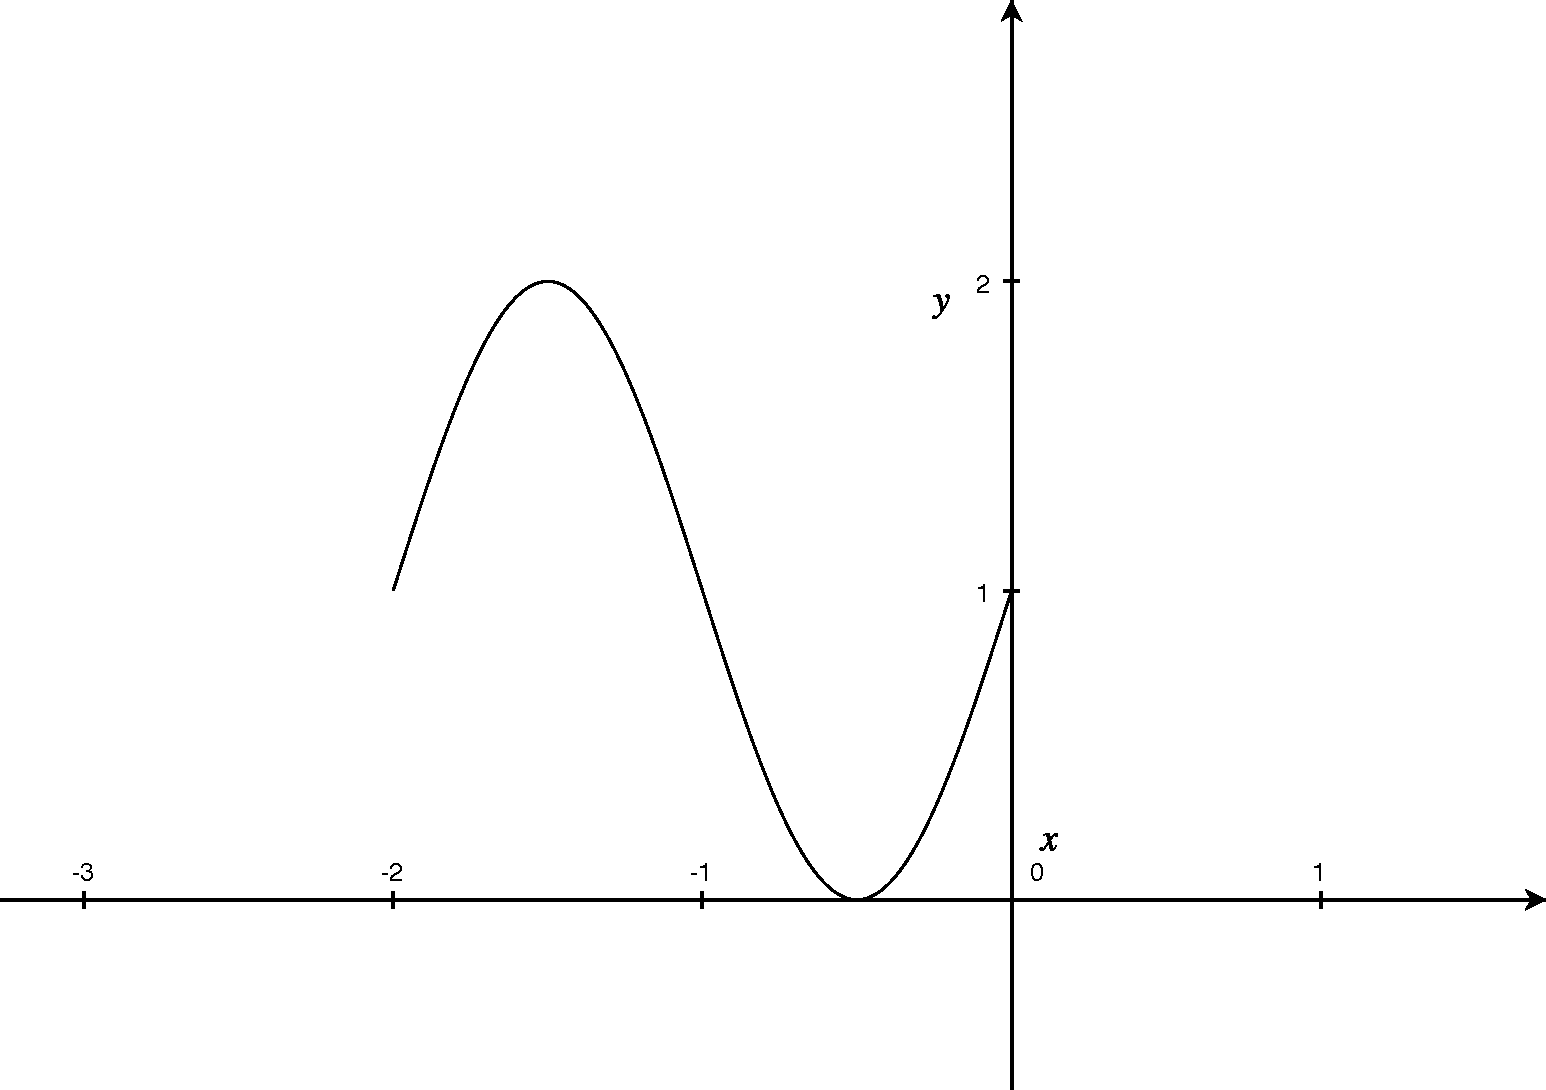
\includegraphics[width=0.5\textwidth]{./graphics/graph101.pdf}
   \caption{Graph of $f \left( x \right) = \sin \left( \pi x + 2 \pi \right) + 1$.}
   \label{fig:graph101}
\end{figure}
% _-_-_-_-_-_-_-_-_-_-_-_-_-_-_-_-_-_-_-_-_-_-_-_-_-_-_-_-_-_-_-_-


% _-_-_-_-_-_-_-_-_-_-_-_-_-_-_-_-_-_-_-_-_-_-_-_-_-_-_-_-_-_-_-_-
\question Perform the indicated addition and use the fundamental identities to simplify.
\[
\frac{1}{1 - \sin x} + \frac{1}{1 + \sin x}
\]
\begin{solution}
\begin{eqnarray*}
\frac{1}{1 - \sin x} + \frac{1}{1 + \sin x} &=& \frac{1}{1 - \sin x} \cdot \frac{1 + \sin x}{1 + \sin x}  + \frac{1}{1 + \sin x} \cdot \frac{1 - \sin x}{1 - \sin x}\\
 &=& \frac{1 + \sin x}{1 - \sin^2 x}  +  \frac{1 - \sin x}{1 - \sin^2 x}\\
  &=& \frac{1 + \sin x + 1 - \sin x}{1 - \sin^2 x}\\
  &=& \frac{2}{1 - \sin^2 x}\\
  &=& \boxed{\frac{2}{\cos^2 x}} = \boxed{2 \sec^2 x}
\end{eqnarray*}
\end{solution}
 %_-_-_-_-_-_-_-_-_-_-_-_-_-_-_-_-_-_-_-_-_-_-_-_-_-_-_-_-_-_-_-_-
\question Write an expression for the $n^{\rm{th}}$ term.
\[
2, \ 1, \frac{8}{9}, \ 1, \ \frac{32}{25}, \ldots
\]
\begin{solution}
By inspection.
\[
\boxed{a_n = \frac{2^n}{n^2}}
\]
\end{solution}
% _-_-_-_-_-_-_-_-_-_-_-_-_-_-_-_-_-_-_-_-_-_-_-_-_-_-_-_-_-_-_-_-
\question Find the sum.
\[
\frac{2\pi}{3} + \frac{\pi}{4} + \frac{\pi}{12} = 
\]
\begin{solution}
\[
\frac{2\pi}{3} + \frac{\pi}{4} + \frac{\pi}{12} = 
\frac{8\pi + 3\pi + \pi}{12} = \boxed{\pi}
\]
\end{solution}
% _-_-_-_-_-_-_-_-_-_-_-_-_-_-_-_-_-_-_-_-_-_-_-_-_-_-_-_-_-_-_-_-
\question If
\[
\sin \alpha =  \displaystyle - \frac{5}{13} \qquad {\rm{and}} \qquad  \cos \beta = \displaystyle  \frac{3}{5},
\]
with both $\alpha$ and $\beta$ are in the fourth quadrant. Find the exact values of the following.

\begin{parts}
\part $\sin \left( \alpha - \beta \right)$
\begin{solution}
\begin{eqnarray*}
\sin \alpha = - \frac{5}{13} \qquad &{\rm{and}}& \qquad \cos \alpha =   \frac{12}{13}\\
\sin \beta  =   -\frac{4}{5} \qquad &{\rm{and}}& \qquad \cos \beta =   \frac{3}{5}\\
\end{eqnarray*}
\begin{eqnarray*}
\sin \left( \alpha - \beta \right) &=& \sin \alpha \ \cos \beta - \sin \beta \ \cos  \alpha \\
&=& \left( - \frac{5}{13} \right) \left( \frac{3}{5} \right) -  \left( -\frac{4}{5} \right) \left( \frac{12}{13} \right)\\
&=& \boxed{\frac{33}{65}}
\end{eqnarray*}
\end{solution}
\part $\cos \left( \alpha - \beta \right)$
\begin{solution}
\begin{eqnarray*}
\cos \left( \alpha - \beta \right) &=& \cos \alpha \ \cos \beta + \sin \alpha \ \sin \beta\\
&=& \left( \frac{12}{13} \right)\left( \frac{3}{5} \right) + \left( - \frac{5}{13} \right) \left( -\frac{4}{5} \right) \\
&=& \boxed{\frac{56}{65}}
\end{eqnarray*}
\end{solution}
\part $\tan \left( \alpha - \beta \right)$
\begin{solution}
\begin{eqnarray*}
\tan \left( \alpha - \beta \right) &=& \frac{ \sin \left( \alpha - \beta \right) }{ \cos \left( \alpha - \beta \right)}\\
&=& \frac{\displaystyle \ \frac{33}{65} \ }{\displaystyle \ \frac{56}{65} \ }\\
&=& \boxed{\frac{33}{56}}
\end{eqnarray*}
\end{solution}
\part $\sin \left( \displaystyle \frac{\alpha}{2} \right)$
\begin{solution} Since $\alpha$ is in the fourth quadrant $\alpha/2$ will be in the second quadrant, which will determine the signs of the half-angle formulas.
$\displaystyle \frac{\alpha}{2}$ is in the second quadrant, so the sine will be positive.
\begin{eqnarray*}
\sin \left( \displaystyle \frac{\alpha}{2} \right) &=& \sqrt{\frac{1-\cos \alpha}{2}}\\
&=& \sqrt{ \frac{ 1 - 12/13 }{2}}\\
&=& \boxed{\frac{1}{\sqrt{26}}}
\end{eqnarray*}
\end{solution}
\part $\cos \left( \displaystyle \frac{\alpha}{2} \right)$
\begin{solution}$\displaystyle \frac{\alpha}{2}$ is in the second quadrant, so the cosine will be negative.
\begin{eqnarray*}
\cos \left( \displaystyle \frac{\alpha}{2} \right) &=& -\sqrt{\frac{1+\cos \alpha}{2}}\\
&=& -\sqrt{ \frac{ 1 + 12/13 }{2}}\\
&=& \boxed{-\frac{5}{\sqrt{26}}}
\end{eqnarray*}
\end{solution}
\part $\tan \left( \displaystyle \frac{\alpha}{2} \right)$
\begin{solution} Just take the ratio of sine over cosine.
\begin{eqnarray*}
\tan \left( \displaystyle \frac{\alpha}{2} \right) &=& \frac{\displaystyle \sin \left( \displaystyle \frac{\alpha}{2} \right)}{\displaystyle \cos \left( \displaystyle \frac{\alpha}{2} \right)}\\
&=& \boxed{-\frac{1}{5}}
\end{eqnarray*}
\end{solution}
\end{parts}
% _-_-_-_-_-_-_-_-_-_-_-_-_-_-_-_-_-_-_-_-_-_-_-_-_-_-_-_-_-_-_-_-
\question Find all solutions.
\[
2 \sin^2 x + 3 \cos x - 3 = 0
\]
\begin{solution} You'll need to write it in terms of cosines first.
\begin{eqnarray*}
2 \sin^2 x + 3 \cos x - 3 &=& 0\\
2 \left( 1 - \cos^2 x \right) + 3 \cos x - 3 &=& 0\\
-2 \cos^2 x  + 3 \cos x - 1 &=& 0
\end{eqnarray*}
Now multiply both sides of this equation by $-1$ and factor.
\begin{eqnarray*}
2\cos^2 x  - 3 \cos x + 1 &=& 0\\
\left(2 \cos x - 1  \right) \left(\cos x - 1 \right) &=& 0
\end{eqnarray*}
Set each factor equal to zero and solve.
\begin{eqnarray*}
\cos x = \frac{1}{2} \qquad \Rightarrow \qquad x &=& \boxed{\frac{\pi}{3} + 2 \pi k, \quad k \in \mathbb{Z}} \\
&=& \boxed{\frac{5\pi}{3} + 2 \pi k, \quad k \in \mathbb{Z}} \\
\cos x = 1 \qquad \Rightarrow \qquad x &=& \boxed{2 \pi k, \quad k \in \mathbb{Z}}.
\end{eqnarray*}
\end{solution}
% _-_-_-_-_-_-_-_-_-_-_-_-_-_-_-_-_-_-_-_-_-_-_-_-_-_-_-_-_-_-_-_-
\question Verify the identity.\footnote{Here it might be nice to mention that $1 + \sin x \geq 0$ so $\sqrt{\left(1 + \sin x\right)^2} = 1 + \sin x$. However, since $-1 \leq \cos x \leq 1$, the $\sqrt{\cos^2 x} = \left| \cos x\right|$.}
\[
\sqrt{\frac{1 + \sin x}{1 - \sin x}} = \frac{1 + \sin x}{\left| \cos x\right|}
\]
\begin{solution}
Select the left side.
\begin{eqnarray*}
\sqrt{\frac{1 + \sin x}{1 - \sin x}} &=& \sqrt{\frac{1 + \sin x}{1 - \sin x} \cdot \frac{1 + \sin x}{1 + \sin x}}\\
&=& \sqrt{\frac{\left(1 + \sin x\right)^2}{1 - \sin^2 x}}\\
&=& \sqrt{\frac{\left(1 + \sin x\right)^2}{\cos^2 x}}\\
&=& \frac{1 + \sin x}{\left| \cos x\right|}
\end{eqnarray*}
\emph{Q.E.D.}
\end{solution}



 %_-_-_-_-_-_-_-_-_-_-_-_-_-_-_-_-_-_-_-_-_-_-_-_-_-_-_-_-_-_-_-_-
\question Rewrite the expression so that it is not in \emph{fractional} form
\[
\frac{\tan^2 x}{\csc x + 1}.
\]
\begin{solution} 
\begin{eqnarray*}
\frac{\tan^2 x}{\csc x + 1} &=& \frac{\tan^2 x}{\displaystyle \frac{1}{\sin x} + 1} \cdot \frac{\sin x }{\sin x }\\
&=& \frac{\tan^2 x \ \sin x}{1 + \sin x} \cdot \frac{1 - \sin x}{1 - \sin x}\\
&=& \frac{\tan^2 x \ \sin x \cdot \left( 1 - \sin x \right)}{1 - \sin^2 x}\\
&=& \frac{\tan^2 x \ \sin x \cdot \left( 1 - \sin x \right)}{\cos^2 x}\\
&=& \boxed{\tan^2 x \ \sin x \cdot \left( 1 - \sin x \right) \cdot \sec^2 x}\\
&=& \boxed{\sin^3 x \cdot \left( 1 - \sin x \right) \cdot \sec^4 x}
\end{eqnarray*}
\end{solution}
% _-_-_-_-_-_-_-_-_-_-_-_-_-_-_-_-_-_-_-_-_-_-_-_-_-_-_-_-_-_-_-_-


% _-_-_-_-_-_-_-_-_-_-_-_-_-_-_-_-_-_-_-_-_-_-_-_-_-_-_-_-_-_-_-_-
\question If $z = -1 - 1 i$, find the trigonometric form of $z$ and $z^9$, also find $z^9$ in standard form.
\begin{solution}
Here $\theta = 225^\circ$ or $\theta = \displaystyle \frac{5\pi}{4}$, and $r = \sqrt{2}$.
\begin{eqnarray*}
z &=& \boxed{\sqrt{2} \cos 225^\circ + \left(\sqrt{2} \sin 225^\circ \right)i}\\
z^9 &=& \boxed{16 \sqrt{2} \cos 2025^\circ + \left( 16 \sqrt{2} \sin 2025^\circ \right) i}\\
z^9 &=& \boxed{ -16 - 16i}
\end{eqnarray*}
\end{solution}

\question Find all solutions.
\[
2 \cos^2 x + 3 \sin x - 3 = 0
\]
\begin{solution} You'll need to write it in terms of cosines first.
\begin{eqnarray*}
2 \cos^2 x + 3 \sin x - 3 &=& 0\\
2 \left( 1 - \sin^2 x \right) + 3 \sin x - 3 &=& 0\\
-2 \sin^2 x  + 3 \sin x - 1 &=& 0
\end{eqnarray*}
Now multiply both sides of this equation by $-1$ and factor.
\begin{eqnarray*}
2\sin^2 x  - 3 \sin x + 1 &=& 0\\
\left(2 \sin x - 1  \right) \left(\sin x - 1 \right) &=& 0
\end{eqnarray*}
Set each factor equal to zero and solve.
\begin{eqnarray*}
\sin x = \frac{1}{2} \qquad \Rightarrow \qquad x &=& \boxed{\frac{\pi}{6} + 2 \pi k, \quad k \in \mathbb{Z}} \\
&=& \boxed{\frac{5\pi}{6} + 2 \pi k, \quad k \in \mathbb{Z}} \\
\sin x = 1 \qquad \Rightarrow \qquad x &=& \boxed{\frac{\pi}{2} + 2 \pi k, \quad k \in \mathbb{Z}}.
\end{eqnarray*}
\end{solution}
% _-_-_-_-_-_-_-_-_-_-_-_-_-_-_-_-_-_-_-_-_-_-_-_-_-_-_-_-_-_-_-_-
\question Find the supplement of $83^\circ$.
\begin{solution}
\[
180^\circ-83^\circ=\boxed{97^\circ}
\]
\end{solution}
% _-_-_-_-_-_-_-_-_-_-_-_-_-_-_-_-_-_-_-_-_-_-_-_-_-_-_-_-_-_-_-_-
\question Solve the triangle, given $a = 11.23$ inches $b = 8.24$ inches, and $B = 29.84^\circ$.
\begin{solution}
You should, of course, draw a triangle first. This one actually gives two distinct answers. I'll give you credit for either one.

\fbox{$A = 42.70^\circ$, $C = 107.46^\circ$ and $c = 15.80$ inches.}

or

\fbox{$A = 137.30^\circ$, $C = 12.86^\circ$ and $c = 3.69$ inches.}
\end{solution}
% _-_-_-_-_-_-_-_-_-_-_-_-_-_-_-_-_-_-_-_-_-_-_-_-_-_-_-_-_-_-_-_-
\question Determine two coterminal angles in radian measure (one positive, one negative) for $\theta = \displaystyle \frac{\pi}{3}$.
\begin{solution}
\[
\frac{\pi}{3} + 2 \pi = \boxed{\frac{7\pi}{3}} \quad {\rm{and}} \quad
\frac{\pi}{3} - 2 \pi = \boxed{-\frac{5\pi}{3}}
\]
\end{solution}
% _-_-_-_-_-_-_-_-_-_-_-_-_-_-_-_-_-_-_-_-_-_-_-_-_-_-_-_-_-_-_-_-
\question Find the length of arc on a circle of radius 14 inches and a central angle of $60^\circ$.
\begin{solution}
\[
S = 14 \cdot \frac{\pi}{3}
\]
So, the length is \fbox{$\displaystyle \frac{14 \pi}{3}$ inches}.
\end{solution}
% _-_-_-_-_-_-_-_-_-_-_-_-_-_-_-_-_-_-_-_-_-_-_-_-_-_-_-_-_-_-_-_-
\question If the $\sec \theta = 7$ and $270^\circ < \theta < 360^\circ$, find the following.
So, $y = -4\sqrt{3}$
\begin{parts}
\part $\sin \theta$
\begin{solution}
From the information given we can conclude that $x= 1$, $r = 7$, and that $y < 0$. To find the value of $y$, solve
\[
7^2 = 1^2 + y^2 \quad \Rightarrow \quad y = \pm \sqrt{48} = \pm 4\sqrt{3}.
\]
$\sin \theta = \boxed{\frac{-4\sqrt{3}}{7}}$
\end{solution}
\part $\cos \theta$
\begin{solution}
$\cos \theta = \boxed{\frac{1}{7}}$
\end{solution}
\part $\tan \theta$
\begin{solution}
$\tan \theta = \boxed{-4\sqrt{3}}$
\end{solution}
\part $\cot \theta$
\begin{solution}
$\cot \theta = \boxed{\frac{-1}{4\sqrt{3}}}$
\end{solution}
\part $\csc \theta$
\begin{solution}
$\csc \theta = \boxed{\frac{-7}{4\sqrt{3}}}$
\end{solution}
\end{parts}
% _-_-_-_-_-_-_-_-_-_-_-_-_-_-_-_-_-_-_-_-_-_-_-_-_-_-_-_-_-_-_-_-
\question Given that
\[
P_k = \frac{k}{2} \cdot \left[ 5k - 3 \right],
\]
find $P_{k+1}$.
\begin{solution} Just replace $k$ with $\left(k + 1 \right)$.
\[
\boxed{P_{k+1} = \frac{\left(k + 1 \right)}{2} \cdot \left[ 5\left(k + 1 \right) - 3 \right]}.
\]
\end{solution}
% _-_-_-_-_-_-_-_-_-_-_-_-_-_-_-_-_-_-_-_-_-_-_-_-_-_-_-_-_-_-_-_-
\end{questions}
\subsection{Assignment}
You should review, as necessary,  the materials presented in Chapter 1 and do the WebAssign assignment mth.121.01.00.
\vfill
\pagebreak
%*-*-*-*-*-*-*-*-*-*-*-*-*-*-*-*-*-*-*-*-*-*-*-*-*-*-*-*-*-*-*-*-*-*-*-*-*-*-*-*-*-*-*-*-*-*-*-*-*-*-*-*-*-*-*-*-*-*-*-*-*-*-*-*-*-*-*-*-*-*-*-*-*-*-*-*-*-*-*-*-*-*-*-*-

\begin{teacher}
\subsection{Assessments}
This is a review of material covered in MTH 119 and 120. There is no need to cover this material in class, and you should advise students not capable of completing this assignment to consider dropping mth 121 until they are able to do do this material. Although this assignment will carry credit, it is not to be used to measure any MPOs for MTH 121.
\begin{questions}
\question 	%RogaCalcET2 1.1.011	WA-1734818
Write the inequality $\left|2x+2\right|<4$ in the form $a<x<b$ for some numbers  $a$, $b$.
\begin{solution}
%\[
%-3<x<1
%\]
\end{solution}

\question 	%RogaCalcET2 1.1.019	WA-1682066
Describe the set as a union of finite or infinite intervals.
\[
\{ x: \left|x - 5\right| > 3\}
\]
\begin{solution}
%\[
%\left( - \infty, \ 2 \right) \cup \left(8, \ \infty \right)
%\]
\end{solution}

\question 	%RogaCalcET2 1.1.024	WA-1737526
Describe the following set as an interval.
\[
\{ x :  \frac{x}{x+5} < 0 \}
\]
\begin{solution}
%\[
%\left( - 5, \ 0 \right)
%\]
\end{solution}

\question 	%RogaCalcET2 1.1.033	WA-1682013
Express $r_1 = 0.\overline {54}$ and $r_2 = 0.4\overline{33}$ as fractions.
\begin{solution}
%\[
%r_1 = \frac{6}{11}, \quad r_2 = \frac{13}{30}
%\]
\end{solution}

\question 	%RogaCalcET2 1.1.037	WA-1734748
Find the equation of the circle with center $\left(2, \ 2\right)$:
\begin{parts}
\part with radius $r = 2$;
\begin{solution}
%\[
%\left( x-2\right)^2 + \left( y-2\right)^2 = 4
%\]
\end{solution}
\part that passes through $\left(1, \ -1\right)$.
\begin{solution}
%\[
%\left( x-2\right)^2 + \left( y-2\right)^2 = 10
%\]
\end{solution}
\end{parts}


\question 	%RogaCalcET2 1.1.046	WA-1737512
Find the domain and range of the function.
\[
f \left( x \right) = \frac{1}{4+x}
\]
\begin{solution}
%The domain is all real numbers except $-4$; the range is all real numbers except $0$.
\end{solution}

\question 	%RogaCalcET2 1.1.055	WA-1682035
Let $f\left(x\right) = x^3 - x$.
\begin{parts}
\part Find the zeros of $f\left(x\right)$.
\begin{solution}
%\[
%x=0, \quad x = \pm 1
%\]
\end{solution}
\part Is $f\left(x\right)$ an odd function?
\begin{solution}
%Yes
\end{solution}
\part Determine the intervals on which $f\left(x\right)$  is positive.
\begin{solution}
\end{solution}
\part Graph $f\left(x\right)$.
\begin{solution}
\end{solution}
\end{parts}



\question 	%RogaCalcET2 1.2.001	WA-1682056

Find the slope, the $y$-intercept, and the $x$-intercept of the line with the given equation.
\[
y = 6x + 12
\]

\begin{solution}
\end{solution}

\question 	%RogaCalcET2 1.2.009	WA-1738327
Find the equation of the line with the given description: slope $4$, $y$-intercept 2.
\begin{solution}
\end{solution}

\question 	%RogaCalcET2 1.2.022	WA-1737537

Find the equation of the line shown (Figure \ref{fig:1737537}, page \pageref{fig:1737537}) below. 
\begin{figure}[htbp] %  figure placement: here, top, bottom, or page
   \centering
   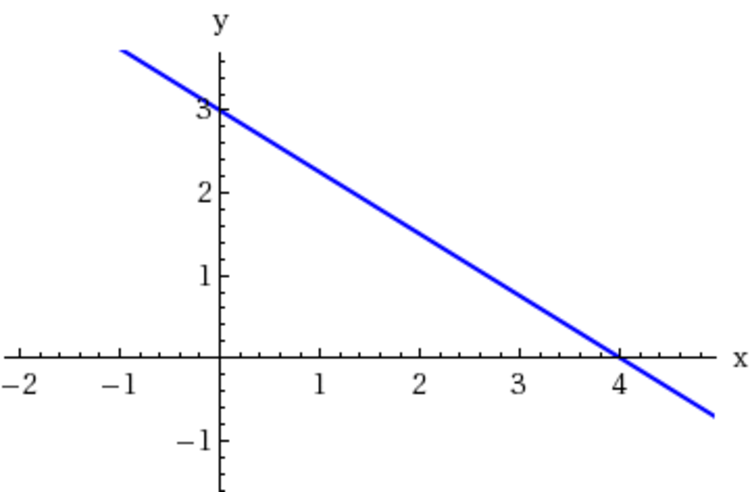
\includegraphics[width=3in]{./graphics/1737537.pdf} 
   \caption{WA-1737537}
   \label{fig:1737537}
\end{figure}

\begin{solution}
\end{solution}

\question 	%RogaCalcET2 1.2.029	WA-1682024
Find $b$ so that the points $\left(5, \ -3\right)$, $\left(6, \ 3 \right)$, and $\left(b, \ 9 \right)$ lie on a line.

\begin{solution}
\end{solution}

\question 	%RogaCalcET2 1.2.033.XP	 WA-1682076

Find the roots of the quadratic polynomial.
\[
6x^2 - 7x - 5
\]

\begin{solution}
\end{solution}

\question 	%RogaCalcET2 1.2.037	WA-1682042

Complete the square and find the minimum or maximum value of the quadratic function.
\[
y = x^2 + 4x + 1
\]

\begin{solution}
\end{solution}

\question 	%RogaCalcET2 1.3.001	WA-1682046

Determine the domain of the function.
\[
f\left(x\right) = x^{1/6}
\]

\begin{solution}
\end{solution}

\question 	%RogaCalcET2 1.3.003	WA-1757401

Determine the domain of the function.
\[
f\left(x\right) = x^3 + 9x - 10
\]

\begin{solution}
\end{solution}

\question 	%RogaCalcET2 1.3.005	WA-1682057

Determine the domain of the function.
\[
g\left(t\right) = \frac{1}{t + 2}
\]

\begin{solution}
\end{solution}

\question 	%RogaCalcET2 1.3.012	WA-1682068

Determine the domain of the function.
\[
f\left(x\right) = \frac{x + x^{-1}}{\left(x - 3\right)\left(x + 8\right)}
\]


\begin{solution}
\end{solution}

\question 	%RogaCalcET2 1.3.026	WA-1682026

Show that $f\left(x\right) = x^2 + 3x^{-1}$ and $g\left(x\right) = 5x^3 - 4x + x^{-2}$ are rational functions by writing each as a quotient of polynomials.
 
 
\begin{solution}
\end{solution}

\question 	%RogaCalcET2 1.3.027	WA-1757382

Calculate the composite functions $f \circ g$ and $g \circ f$, and determine their domains.
\[
f\left(x\right) = \sqrt{x}, \quad g\left(x\right) = x + 2
\]

\begin{solution}
\end{solution}

\question 	%RogaCalcET2 1.3.036	WA-1682065

Find all values of $c$ such that the domain of
\[ 
f\left(x\right) = \frac{x + 5}{x^2 + 2cx + 25}
\]
is $\mathbb{R}$ (all real numbers).
 
 
\begin{solution}
\end{solution}

\question 	%RogaCalcET2 1.4.042	WA-1739455

Solve $\sin \theta = \sin 2 \theta$ for $\pi \leq \theta  < 2 \pi$.
 
\begin{solution}
\end{solution}



\question 	%RogaCalcET2 1.4.057	WA-1758500

Use the Law of Cosines to find the distance from $P$ to $Q$ in the figure (Figure \ref{fig:1758500}, page \pageref{fig:1758500}) below if $a = 17$, $b = 8$. (Round your answer to four decimal places.)
 
 \begin{figure}[htbp] %  figure placement: here, top, bottom, or page
    \centering
    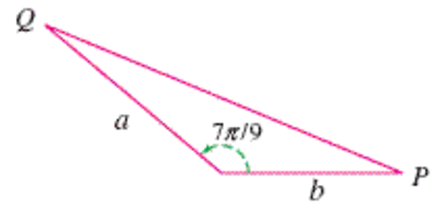
\includegraphics[width=3in]{./graphics/1758500.pdf} 
    \caption{WA-1758500}
    \label{fig:1758500}
 \end{figure}
\begin{solution}
\end{solution}

\question 	%RogaCalcET2 1.5.002	WA-1758482

Is $f\left(x\right) = x^2 + 3$ one-to-one?
 
\begin{solution}
\end{solution}

\question 	%RogaCalcET2 1.5.004	WA-1739549

Consider the following function.
\[
f\left(x\right) = \frac{x-2}{x+2}
\]
\begin{parts}
\part Show that $f\left(x\right)$ is invertible by finding its inverse.
\begin{solution}
\end{solution}
\part  What is the domain of $f\left(x\right)$?
\begin{solution}
\end{solution}
\part What is the range of $f^{-1}\left(x\right)$?
\begin{solution}
\end{solution}
\part What is the domain of $f^{-1}\left(x\right)$?
\begin{solution}
\end{solution}
\part What is the range of $f\left(x\right)$?
\begin{solution}
\end{solution}
\end{parts}



\question 	%RogaCalcET2 1.5.027	WA-1758477

Evaluate without using a calculator.
\[
\tan^{-1} 1
\]


\begin{solution}
\end{solution}

\question 	%RogaCalcET2 1.5.028	WA-1758521

Evaluate without using a calculator.
\[
\sin^{-1} 1
\]

\begin{solution}
\end{solution}

\question 	%RogaCalcET2 1.5.030	WA-1739461

Compute the value of the given function without using a calculator.
\[
\arccos \left( \cos \frac{4\pi}{3} \right)
\]


\begin{solution}
\end{solution}

\question 	%RogaCalcET2 1.5.039	WA-1682014


Simplify by referring to the appropriate triangle or trigonometric identity.
\[
\tan \left( \cos^{-1} x \right)
\]

\begin{solution}
\end{solution}

\question 	%RogaCalcET2 1.6.003	WA-1682061


Solve for the unknown variable.
\[
e^{9x} = e^{x + 4}
\]
\begin{solution}
\end{solution}

\question 	%RogaCalcET2 1.6.005	WA-1759367

Solve for the unknown variable.
\[
3^x = \left( \frac{1}{3} \right)^{x+8}
\]

\begin{solution}
\end{solution}

\question 	%RogaCalcET2 1.6.011	WA-1682063

Calculate directly (without using a calculator).
\[
\log_2 4
\]

\begin{solution}
\end{solution}

\question 	%RogaCalcET2 1.6.018	WA-1759433

Calculate directly (without using a calculator).
\[
\log_2 8^2
\]

\begin{solution}
\end{solution}

\question 	%RogaCalcET2 1.6.020	WA-1759363


Calculate directly (without using a calculator).
\[
\log_{25} 30 + \log_{25} \frac{1}{6}
\]




\begin{solution}
\end{solution}

\question 	%RogaCalcET2 1.6.028	WA-1739573

Solve for $x$.
\[
\ln \left(7x^2 + 4\right) - 3 \ln x = \ln 4
\]

\begin{solution}
\end{solution}

\end{questions}
\end{teacher}
\vfill
\pagebreak
%*-*-*-*-*-*-*-*-*-*-*-*-*-*-*-*-*-*-*-*-*-*-*-*-*-*-*-*-*-*-*-*-*-*-*-*-*-*-*-*-*-*-*-*-*-*-*-*-*-*-*-*-*-*-*-*-*-*-*-*-*-*-*-*-*-*-*-*-*-*-*-*-*-*-*-*-*-*-*-*-*-*-*-*-













%*-*-*-*-*-*-*-*-*-*-*-*-*-*-*-*-*-*-*-*-*-*-*-*-*-*-*-*-*-*-*-*-*-*-*-*-*-*-*-*-*-*-*-*-*-*-*-*-*-*-*-*-*-*-*-*-*-*-*-*-*-*-*-*-*-*-*-*-*-*-*-*-*-*-*-*-*-*-*-*-*-*-*-*-
\section{mth.121.02.01}

\subsection{Tangents and Secants}

The idea of a limit is central to calculus and an intuitive grasp of this concept is essential to further study. Initially we will examine two special types of limits: tangents and velocities. These two limits gives rise to the central idea in differential calculus---the derivative.

The word tangent is derived from the Latin word \emph{tangens}, which means `touching.' Thus, a tangent to a curve is a line that touches the curve and has the same direction as the curve at the point of contact.

Let's take a look at the curve\footnote{Make sure you can graph simple functions by hand, however, more difficult graphs may require the use of technology. Make sure you know how to graph both simple and more difficult functions.} (Figure \ref{fig:graph0201}, page \pageref{fig:graph0201}) $\displaystyle y = \frac{x^3}{3} -\frac{x^2}{2} - 2x + 5$  and a line $y=-2x+5$, which is tangent to this curve at the point $\left( 0, \ 5 \right)$.
\begin{figure}[htbp] %  figure placement: here, top, bottom, or page
   \centering
   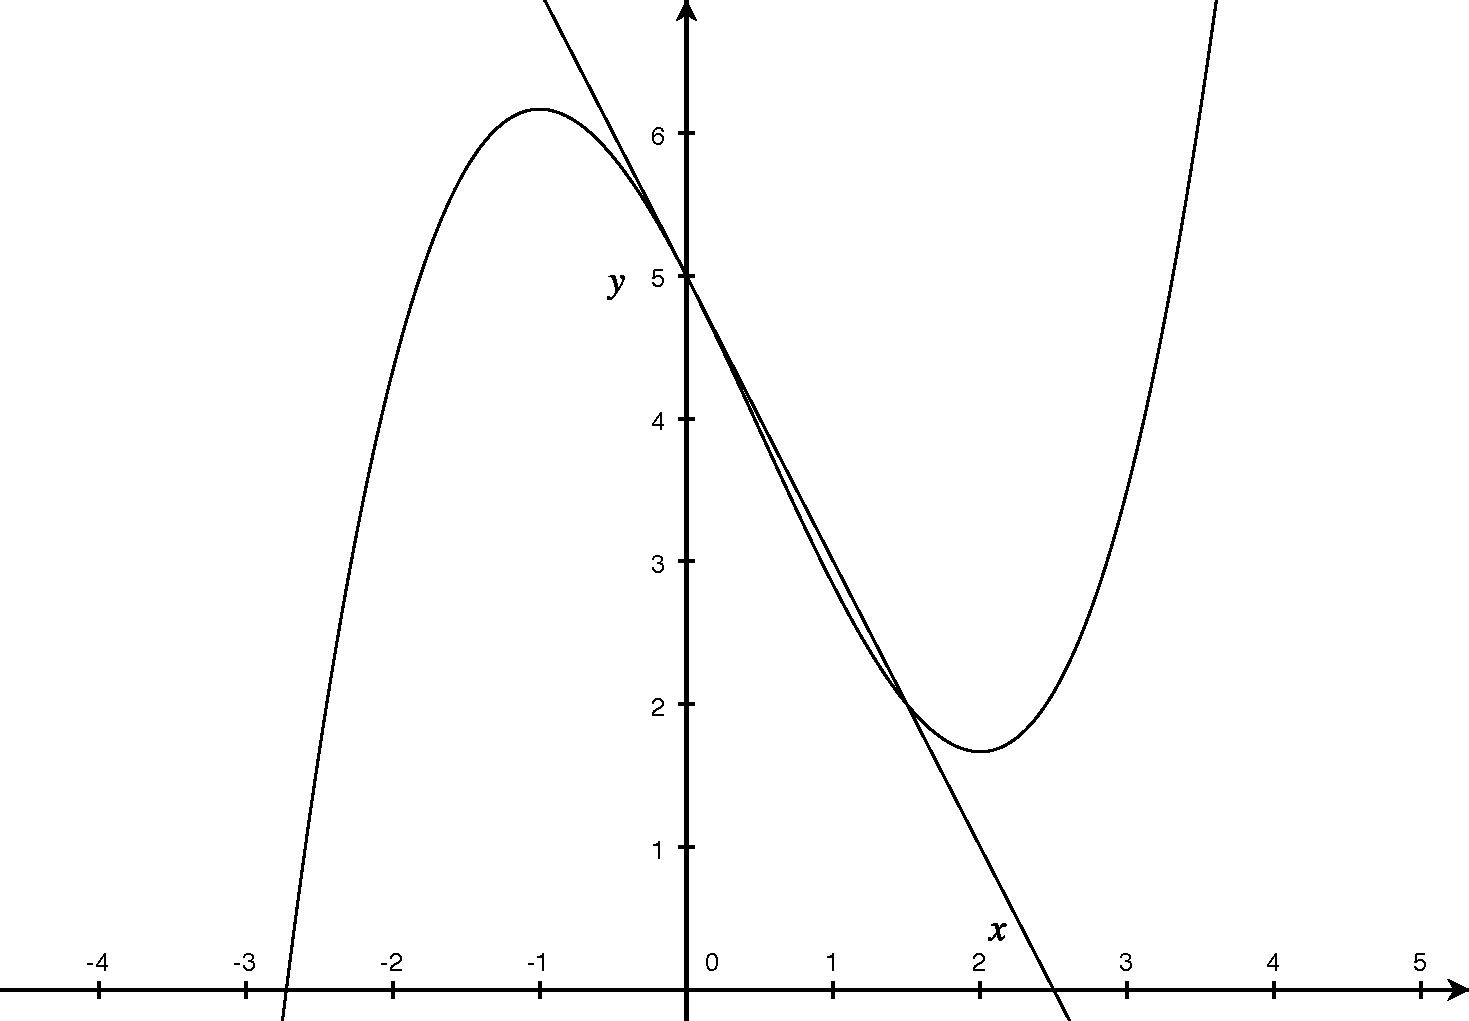
\includegraphics[width=4in]{./graphics/graph0201.pdf} 
   \caption{$\displaystyle y = \frac{x^3}{3} -\frac{x^2}{2} - 2x + 5$ and $y=-2x+5$ }
   \label{fig:graph0201}
\end{figure}

This particular tangent line also happens to be a secant line,\footnote{A secant is a straight line that cuts a curve in two or more parts. A tangent is a straight line that touches a curve at a point, but does not cross (some say puncture) it at that point. There's \emph{subtlety} here, because you can have a line that touches and does not puncture  a curve at a point, but is not tangent. We'll more precisely define tangent later.} because it touches this particular curve twice.\footnote{You should be able to visually note that there are at least two points of intersection, but can you show that there's only two? What are the two points?} Again, take a look!

\textbf{Example:} Let's take a look at a very simple example. Find an equation of the tangent line to the parabola $y = x^2$ at the point $P\left( 1, \ 1 \right)$.


\begin{figure}[htbp] %  figure placement: here, top, bottom, or page
   \centering
   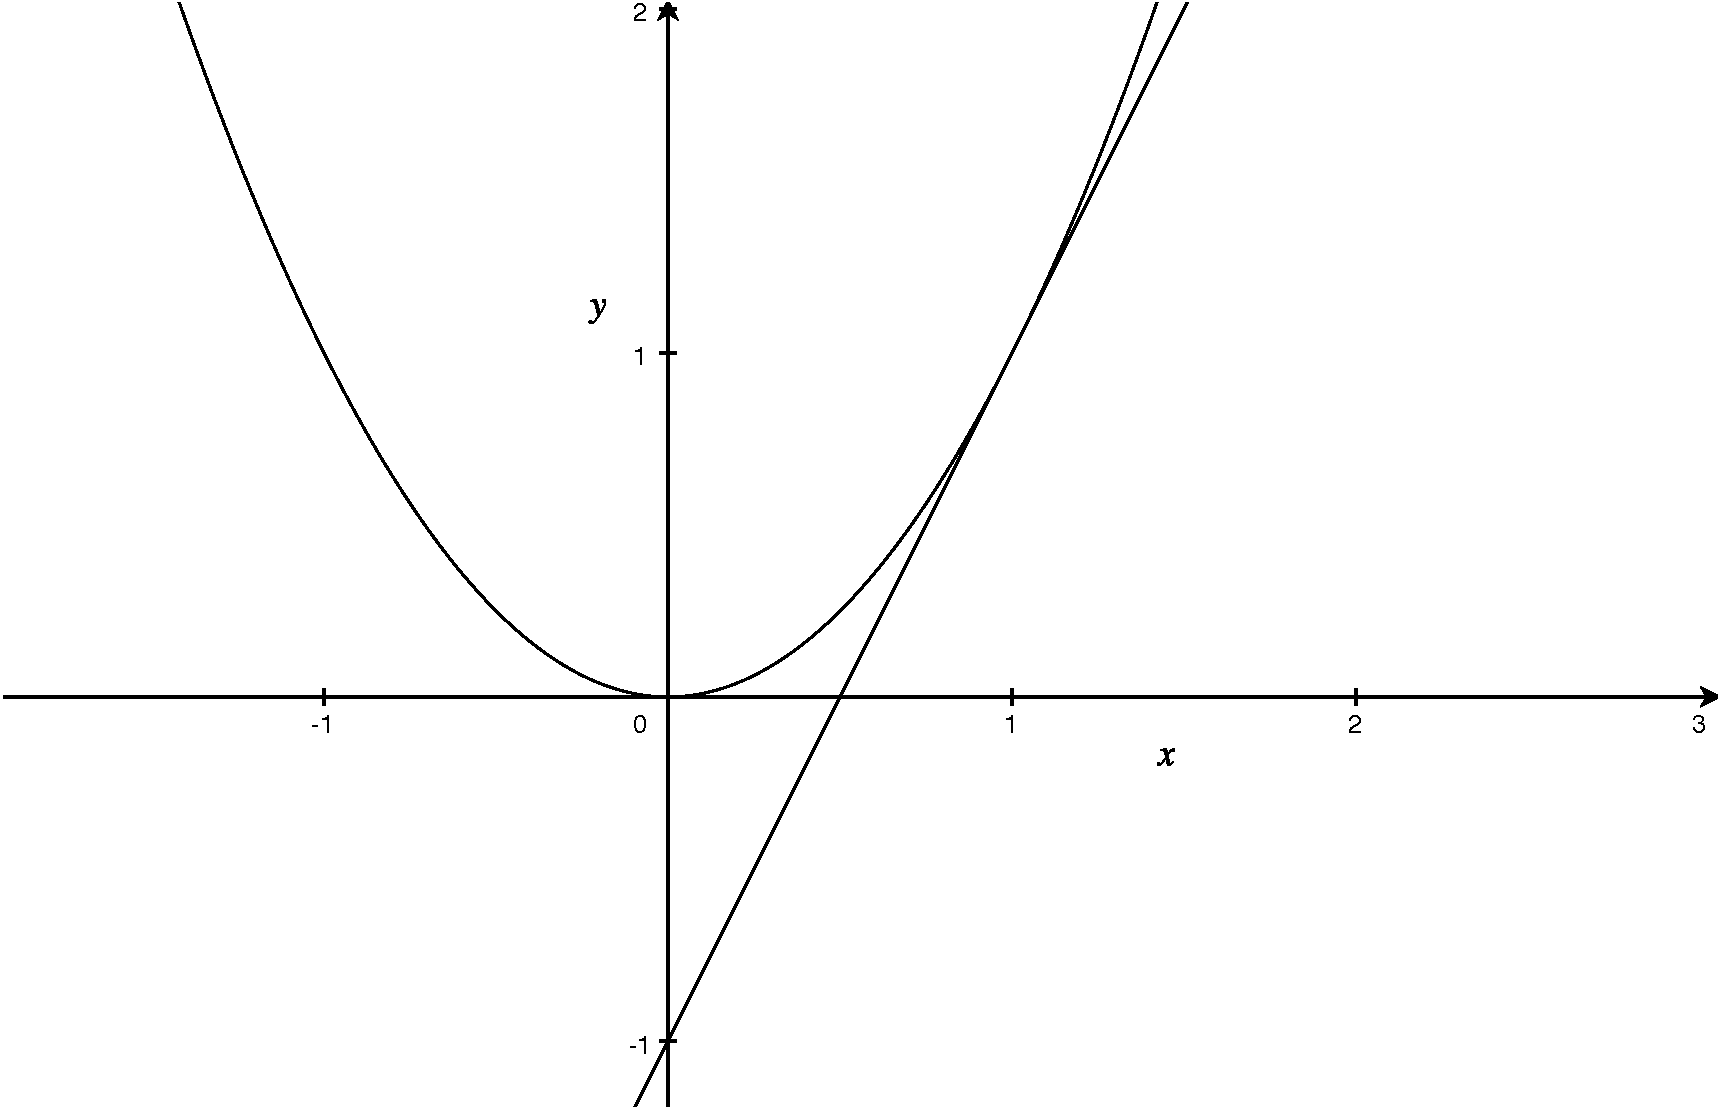
\includegraphics[width=4in]{graphics/graph020101.pdf} 
   \caption{$y=x^2$ and a line tangent at $P\left( 1, \ 1 \right)$.}
   \label{fig:graph020101}
\end{figure}
\begin{solution}
First we will make a rough sketch (Figure \ref{fig:graph020101}, page \pageref{fig:graph020101}) and then try to make a guess at what this tangent line is. A good guess (slope \emph{appears} to be $m=2$ and the $y$-intercept \emph{appears} to be $b =-1$) for the equation of the line tangent is:
\[
y = 2x -1.
\]
Your answer may vary depending on how accurate your graph is.

Next we will take a sequence of secant lines that approach the tangent line, compute their slopes---this is often referred to as \emph{rate of change}, or simply ROC---and make a prediction where these slopes are going. Since we want to move towards the point $P\left( 1, \ 1 \right)$, along the curve $y = x^2$, we can select points from both the right and left of $P$ and compute the slope of the secant line using the slope formula. Let's not be timid (stay close) when choosing values to the right and left of $x=1$. Here's a nice pattern for the right of $x=1$: $1.1, 1.01, 1.001$; now lets compute the slope of the secant using $P\left( 1, \ 1 \right)$ for these three values for $x$.

From the \emph{right} of $x=1$.
\begin{eqnarray*}
m_{\mbox{secant}} \left( x \right) &=& \frac{x^2-1}{x-1} = x+1, \quad x \neq 1\\
m_{\mbox{secant}} \left( 1.1 \right) &=& 2.1\\
m_{\mbox{secant}} \left( 1.01 \right) &=& 2.01\\
m_{\mbox{secant}} \left( 1.001 \right) &=& 2.001
\end{eqnarray*}
Looks like this sequence is going towards $2$. Now from the \emph{left} of $x=1$.
\begin{eqnarray*}
m_{\mbox{secant}} \left( x \right) &=& \frac{x^2-1}{x-1} = x+1, \quad x \neq 1\\
m_{\mbox{secant}} \left( 0.9 \right) &=& 1.9\\
m_{\mbox{secant}} \left( 0.99 \right) &=& 1.99\\
m_{\mbox{secant}} \left( 0.999 \right) &=& 1.999
\end{eqnarray*}
Again, it looks like this sequence is going towards $2$. So now we have a point $P\left( 1, \ 1 \right)$ and an apparent slope $m=2$ of the tangent.
\begin{eqnarray*}
y - 1 &=& 2 \left( x -1 \right)\\
y  &=& 2x -1 
\end{eqnarray*}
Just as we expected!
\end{solution}

\textbf{Example:} This time we will look at a function that has units. Suppose that an object is dropped from a platform that is 400 meters above the ground, and its position ($s$ in meters) above the ground is a function of time ($t$ is seconds), where
\[
s = s \left( t \right) = -4.9 t^2 + 400.
\]
Clearly this is a parabola, and if we draw (Figure \ref{fig:graph020102}, page \pageref{fig:graph020102}) a tangent line at the point where $t=5$, we will be able to approximate the slope.\footnote{I know, it's more difficult because of the scale and units.}
\begin{figure}[htbp] %  figure placement: here, top, bottom, or page
   \centering
   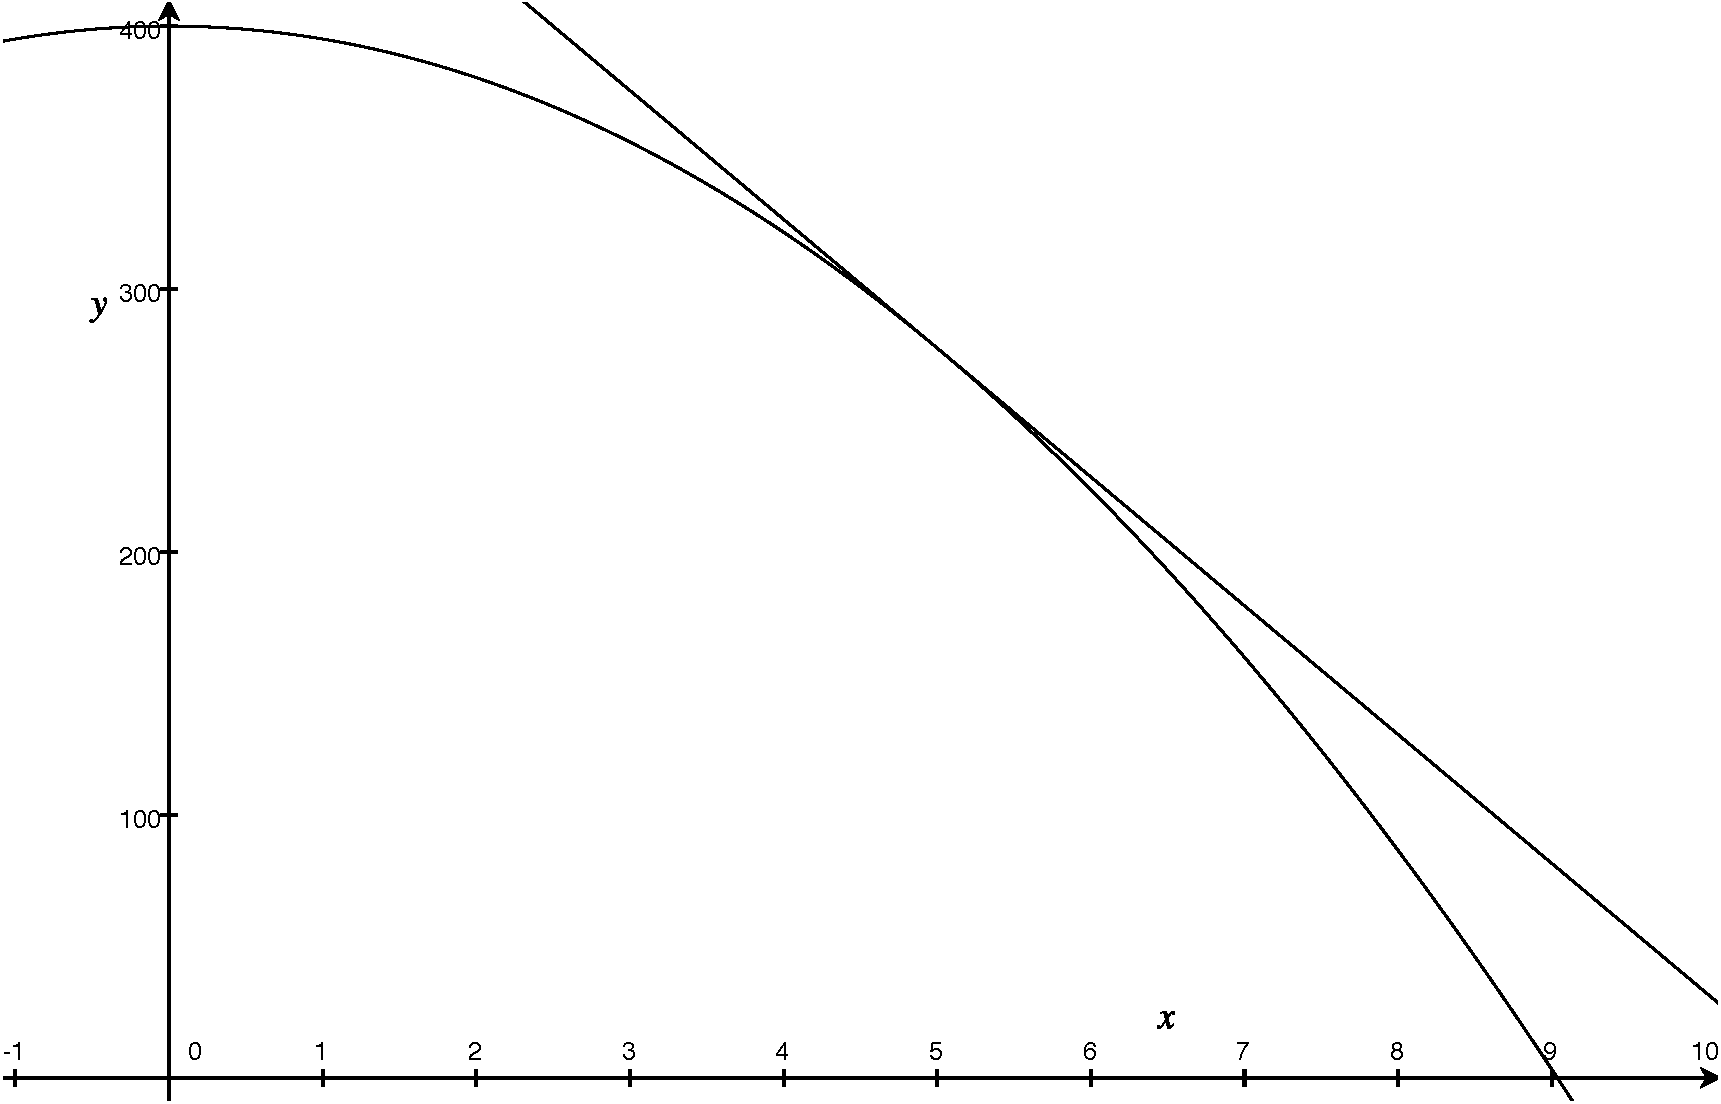
\includegraphics[width=4in]{graphics/graph020102.pdf} 
   \caption{$s = s \left( t \right) = -4.9 t^2 + 400$ and a line tangent at $t=5$.}
   \label{fig:graph020102}
\end{figure}
\begin{enumerate}
\item What is the unit of this slope?

\begin{solution}
Meters per second.
\end{solution}
\item What is the sign of this slope?

\begin{solution}
Negative.
\end{solution}

\item Using $t=5$, find values to the left and right of $t=5$, compute the corresponding slope of the secant lines, and make a prediction about what the slope of the tangent line at this point.\



\begin{solution}
From the \emph{right} of $t=5$.
\begin{eqnarray*}
m_{\mbox{secant}} \left( t \right) &=& \frac{-4.9 t^2 +122.5 }{t-5}, \quad t \neq 5\\
m_{\mbox{secant}} \left( 5.1 \right) &=& -49.49\\
m_{\mbox{secant}} \left( 5.01 \right) &=& -49.049\\
m_{\mbox{secant}} \left( 5.001 \right) &=& -49.0049
\end{eqnarray*}
Looks like this is going towards $-49$.

From the \emph{left} of $t=5$.
\begin{eqnarray*}
m_{\mbox{secant}} \left( t \right) &=& \frac{-4.9 t^2 +122.5 }{t-5}, \quad t \neq 5\\
m_{\mbox{secant}} \left( 4.9 \right) &=& -48.51\\
m_{\mbox{secant}} \left( 4.99 \right) &=& -48.951\\
m_{\mbox{secant}} \left( 4.999 \right) &=& -48.9951
\end{eqnarray*}
Looks like this is also going towards $-49$.

Prediction is $-49$ meters per second.
\end{solution}

\item What is the equation of this tangent line?
\begin{solution}
\begin{eqnarray*}
s-s_1 &=& m \left( t - t_1\right)\\
s - 277.5 &=& -49 \left( t - 5 \right)\\
s &=& -49 t + 522.5
\end{eqnarray*}
\end{solution}

\item What is the \emph{instantaneous velocity} of this object at $t=5$ seconds?

\begin{solution}
The slope of the tangent line for this problem is the same as the \emph{instantaneous velocity}. So the \emph{instantaneous velocity} of this object at $t=5$ seconds is $-49$ meters per second. Yes, the object has negative velocity because it is \emph{falling} towards earth.
\end{solution}

\end{enumerate}

You're going to have to become comfortable with doing these types of computations, and please consider mastering the use of your calculator to facilitate this process.



\subsection{Examples}
\begin{questions}
\question Compute $\displaystyle \frac{\Delta y}{\Delta x}$  for the interval $\left[-1,\ 2\right]$, where $y\left( x \right) = 3x^2 - 2x + 5$. This is just the slope of the secant line through the points $\left( y\left( 2 \right), \ 2 \right)$ and $\left( y\left( -1 \right), \ -1 \right)$.

\begin{solution}
We'll discuss this in class.

\begin{eqnarray*}
\frac{\Delta y}{\Delta x} &=& \frac{y_2 - y_1}{x_2-x_1} = \frac{y\left(x_2\right) - y\left(x_1\right)}{x_2-x_1}\\
&=& \frac{y\left(2\right) - y\left(-1\right)}{2+1}\\
&=& \frac{13 - 10}{3}\\
&=&1
\end{eqnarray*}
\end{solution}

\question Estimate the instantaneous rate of change of the function $y\left( x \right) = 3x^2 - 2x + 5$ at the point $x = -1$.
\begin{solution}
We'll discuss this in class.

You need to make sure you understand the examples presented in class to do this problem. You will not be given credit unless you \emph{know} the proper steps. That is, computing a sequence to secants from both the left and right of $x=-1$, and then making a prediction about what these slopes are converging to.

Final answer: $-8$.
\end{solution}

\question With an initial deposit of $100$ dollars, the balance in a bank account after $t$ years is $f\left(t\right) = 100\left(1.05\right)^t$ dollars.
\begin{figure}[htbp] %  figure placement: here, top, bottom, or page
   \centering
   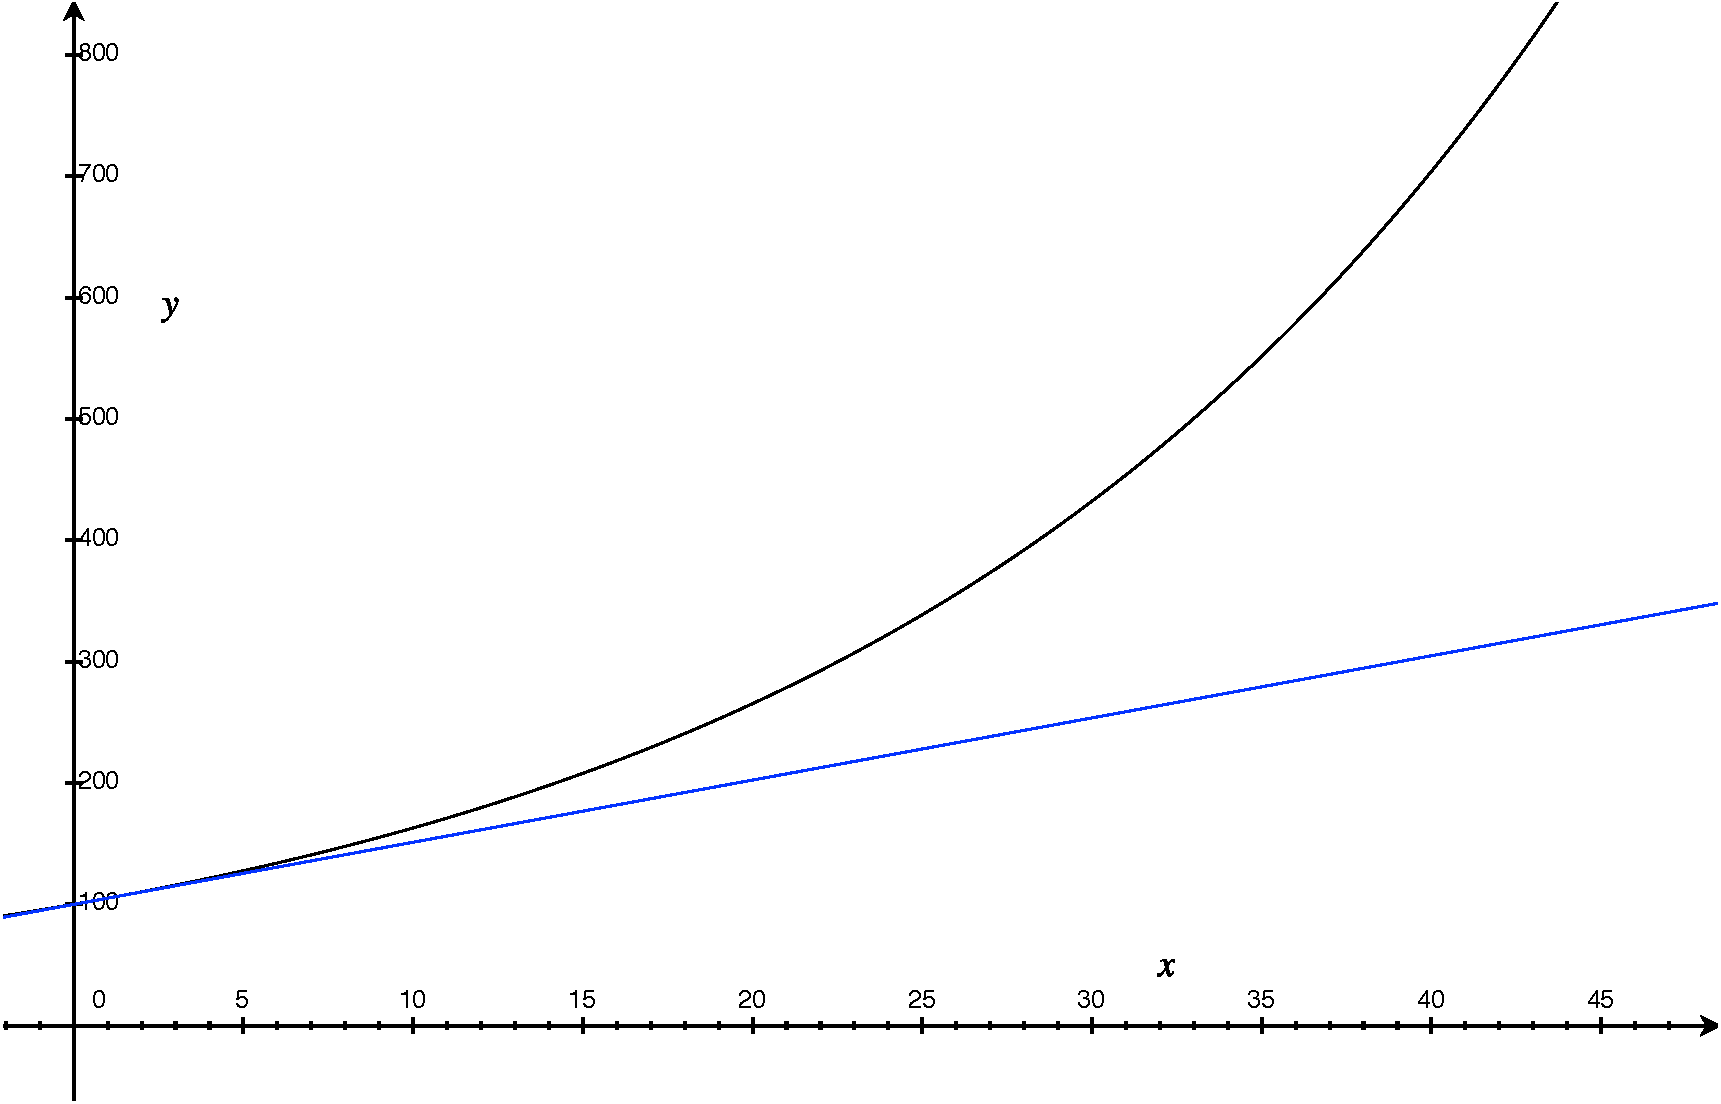
\includegraphics[width=4in]{./graphics/graph_money.pdf} 
   \caption{The growth of money with tangent at $t=1$.}
   \label{fig:graph_money}
\end{figure}
\begin{parts}
\part What are the units of the ROC\footnote{ROC = rate of change} of $f\left(t\right)$?

\begin{solution}
We'll discuss this in class.

Dollars per year.
\end{solution}

\part Graph\footnote{Again, make sure you can graph on your own!} (Figure \ref{fig:graph_money}, page \ref{fig:graph_money}) this functions and estimate the slope of the tangent at $t=1$.

\begin{solution}
We'll discuss this in class.

About $5.1$ dollars per year.
\end{solution}

\part Looking at the graph do the slopes of the tangents appear to be getting bigger as time goes on?

\begin{solution}
We'll discuss this in class.

Yes!
\end{solution}

\end{parts}


\end{questions}
\subsection{Assignment}
You should read \S  2.1 and do the WebAssign assignment mth.121.02.01.
\vfill
\pagebreak
%*-*-*-*-*-*-*-*-*-*-*-*-*-*-*-*-*-*-*-*-*-*-*-*-*-*-*-*-*-*-*-*-*-*-*-*-*-*-*-*-*-*-*-*-*-*-*-*-*-*-*-*-*-*-*-*-*-*-*-*-*-*-*-*-*-*-*-*-*-*-*-*-*-*-*-*-*-*-*-*-*-*-*-*-
\begin{teacher}
\subsection{Assessments}
The following questions are related to the WebAssign assignments and may be used to assess students' ability. Please do not share any of these questions with students.
\begin{questions}		
\question 	%RogaCalcET2 2.1.002	WA-1718621

A wrench released from a state of rest at time $t = 0$ travels a distance $s\left( t \right) = 4.9t^2$ m in $t$ seconds. Estimate the instantaneous velocity $v$ at $t = 8$ seconds. (Round your answer to three decimal places.)

\begin{solution}
%$78.400$ m/sec
\end{solution}

\question 	%RogaCalcET2 2.1.004	WA-1718585

Compute $\displaystyle \frac{\Delta y}{\Delta x}$  for the interval $\left[2,\ 8\right]$, where $y = 3x - 1$.

\begin{solution}
%$3$
\end{solution}


What is the instantaneous rate of change of $y$ with respect to $x$ at 
$x = 6$?


\begin{solution}
%$3$
\end{solution}

\question 	%RogaCalcET2 2.1.005	WA-1701019

A stone is tossed in the air from ground level with an initial velocity of $15$ m/s. It's height at time $t$ is 
$h\left(t\right) = 15t - 4.9t^2$ m.


Compute the stone's average velocity over the time interval $\left[0.5, \ 2.5 \right]$.
\begin{solution}
%ANSWER
\end{solution}

\question 	%RogaCalcET2 2.1.007	WA-1689432

With an initial deposit of $200$ dollars, the balance in a bank account after $t$ years is $f\left(t\right) = 200\left(1.18\right)^t$ dollars.

What are the units of the ROC\footnote{ROC = rate of change} of $f\left(t\right)$?

\begin{solution}
%ANSWER
\end{solution}

\question 	%RogaCalcET2 2.1.011	WA-1700967

Let $P\left(x\right) = 8x^2 - 4$. Estimate the instantaneous rate of change of this function at the point $x = 2$. (Round your answer to the nearest whole number.)
 
\begin{solution}
%ANSWER
\end{solution}

\question 	%RogaCalcET2 2.1.014	WA-1701054

Estimate the instantaneous rate of change of the function $y\left(t\right) = \sqrt{6t + 7}$ at the point $t = 1$. (Round your answer to three decimal places.)
\begin{solution}
%ANSWER
\end{solution}

\question 	%RogaCalcET2 2.1.016	WA-1700958

Estimate the instantaneous rate of change of the function $f\left(x\right) = 9e^x$ at the point $x = e$.
 (Round your answer to three decimal places.)
\begin{solution}
%ANSWER
\end{solution}

\question 	%RogaCalcET2 2.1.017	WA-1700975

Estimate the instantaneous rate of change at the point $x = 7$, for $f\left(x\right) = \ln x$. (Round your answer to three decimal places.)
\begin{solution}
%ANSWER
\end{solution}

\question 	%RogaCalcET2 2.1.018	WA-1700979

Estimate the instantaneous rate of change of function $f\left(x\right) = 3 \arctan x$ at the point $x = \pi/4$.
 (Round your answer to three decimal places.)

\begin{solution}
%ANSWER
\end{solution}

\question 	%RogaCalcET2 2.1.022	WA-1739342

The graphs (Figure \ref{fig:1739342}, page \pageref{fig:1739342}) in the figure below represent the positions of moving particles as a function of time.
\begin{figure}[htbp] %  figure placement: here, top, bottom, or page
   \centering
   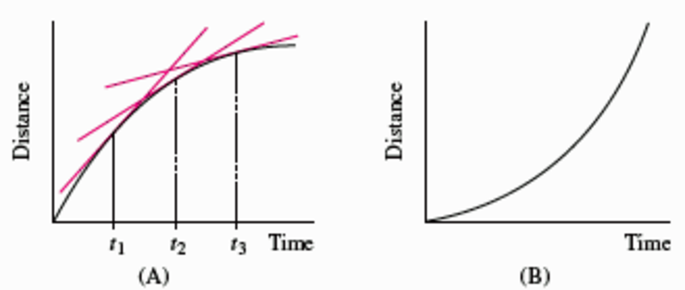
\includegraphics[width=4in]{./graphics/1739342.pdf} 
   \caption{WA-1739342}
   \label{fig:1739342}
\end{figure}
\begin{parts}
\part Do the instantaneous velocities at times $t_1$, $t_2$, $t_3$ in (A) form an increasing or decreasing, or a constant sequence? 
\begin{solution}
%ANSWER
\end{solution}
\part Is the particle speeding up or slowing down or moving at constant speed in (A). 
\begin{solution}
%ANSWER
\end{solution}
\part Is the particle speeding up or slowing down or moving at constant speed in (B). 
\begin{solution}
%ANSWER
\end{solution}
\end{parts}

\question 	%RogaCalcET2 2.1.025	WA-1701013

See problem 25 in \S 2.1.
\begin{solution}
%ANSWER
\end{solution}

\question 	%RogaCalcET2 2.1.030	WA-1701005

Consider the function of the following graph (Figure \ref{fig:1701005}, page \pageref{fig:1701005}). (Round your answers to two decimal places.)
\begin{figure}[htbp] %  figure placement: here, top, bottom, or page
   \centering
   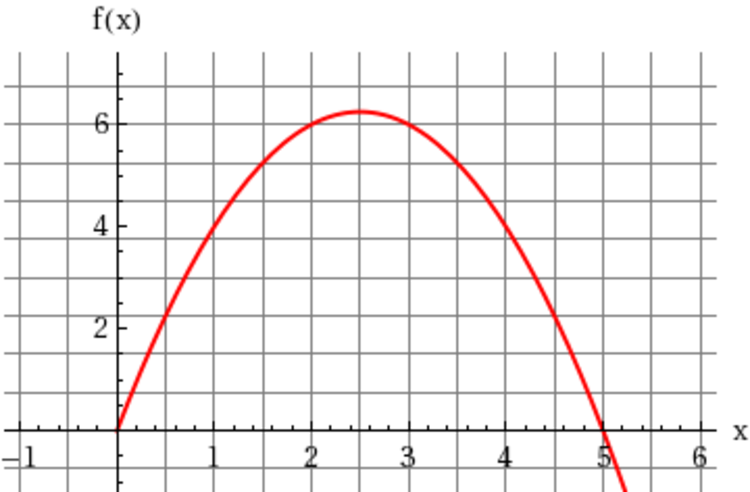
\includegraphics[width=3in]{./graphics/1701005.pdf} 
   \caption{WA-1701005}
   \label{fig:1701005}
\end{figure}
\begin{parts}
\part Find the average rate of change over [0, 5].
\begin{solution}
%ANSWER
\end{solution}
\part Find the instantaneous rate of change at $x = 2.5$.
\begin{solution}
%ANSWER
\end{solution}
\part Choose the values of $x$ at which the rate of change is positive.
\begin{choices}
\choice $\left(0, \ 2.5\right)$
\choice $\left(2.5, \ 5\right)$    
\choice $\left(0, \ 5\right)$
\choice never
\end{choices}
\end{parts}
\begin{solution}
%ANSWER
\end{solution}
\end{questions}
\end{teacher}
\vfill
\pagebreak
%*-*-*-*-*-*-*-*-*-*-*-*-*-*-*-*-*-*-*-*-*-*-*-*-*-*-*-*-*-*-*-*-*-*-*-*-*-*-*-*-*-*-*-*-*-*-*-*-*-*-*-*-*-*-*-*-*-*-*-*-*-*-*-*-*-*-*-*-*-*-*-*-*-*-*-*-*-*-*-*-*-*-*-*-







%*-*-*-*-*-*-*-*-*-*-*-*-*-*-*-*-*-*-*-*-*-*-*-*-*-*-*-*-*-*-*-*-*-*-*-*-*-*-*-*-*-*-*-*-*-*-*-*-*-*-*-*-*-*-*-*-*-*-*-*-*-*-*-*-*-*-*-*-*-*-*-*-*-*-*-*-*-*-*-*-*-*-*-*-
\section{mth.121.02.02}



\subsection{Introductory Limits}

\textbf{Definition:} We write
\[
\mathop {\lim }\limits_{x \to a }  f \left( x \right) = L
\]
and say, ``the limit of $f \left( x \right)$, as $x$ approaches $a$, equals $L$,'' if we can make the values of $f \left( x \right)$ arbitrarily close to $L$ (as close to $L$ as we like) by taking $x$ to be sufficiently close to $a$ (on either side of $a$) but not equal to $a$.




\subsubsection{Calculating Limits}


Although initially difficult to grasp,
\[
\mathop {\lim }\limits_{x \to a}  f \left( x \right),
\]
this notation basically tells us to get close to $a$ (BUT DO NOT TOUCH $a$!). In a way, we are deifying $a$. Fact is, when you tell someone of a forbidden fruit, they want to touch it. But be warned, try not to touch it! If this notation says anything, it says, ``do not touch $a$, but please try to get close to $a$. As close as you like!'' Since $a$ exist on a one dimensional number line, you should note that there are two ways to approach any finite $a$.



We write\footnote{Some do not write the $a^{\pm} $, they write $a{\pm} $ instead.}
\[
\mathop {\lim }\limits_{x \to a^- }  f \left( x \right) = L
\]
and say that the \textbf{left-hand limit} of $f \left( x \right)$ as $x$ approaches $a$ is equal to $L$. A left hand limit just means that we are approaching $a$ from the left, or from values smaller than $a$. We can also write
\[
\mathop {\lim }\limits_{x \to a^+ }  f \left( x \right) = L
\]
and say that the \textbf{right-hand limit} of $f \left( x \right)$ as $x$ approaches $a$ is equal to $L$. A right hand limit just means that we are approaching $a$ from the right, or from values larger than $a$. For the limit
\[
\mathop {\lim }\limits_{x \to a }  f \left( x \right)
\]
to exist, both the left and right limits must exist and be the same. That is
\[
\mathop {\lim }\limits_{x \to a }  f \left( x \right) = L \quad \mbox{if and only if} \quad \mathop {\lim }\limits_{x \to a^- }  f \left( x \right) = L \quad \mbox{and} \quad \mathop {\lim }\limits_{x \to a^+ }  f \left( x \right) = L
\]
You should note that $L$ is referring to a single finite number. If $L$ is not finite, we say the limit does not exists. However, most mathematicians accept the following definitions.
\begin{description}
\item[$L \rightarrow \infty$:] Let $f$ be a function defined on both sides of $a$, except possibly at $a$ itself. Then
\[
\mathop {\lim }\limits_{x \to a }  f \left( x \right) = \infty
\]
means that the value of $f\left(x\right)$ can be made arbitrarily large (as large as we please) by taking $x$ sufficiently close to $a$, but not equal to $a$.
\item[$L \rightarrow  -\infty$:] Let $f$ be a function defined on both sides of $a$, except possibly at $a$ itself. Then
\[
\mathop {\lim }\limits_{x \to a }  f \left( x \right) = -\infty
\]
means that the value of $f\left(x\right)$ can be made arbitrarily large negative by taking $x$ sufficiently close to $a$, but not equal to $a$.
\end{description}



We can also allow $x$ to approach $\pm \infty$, basically to analyze a function's behavior in the extremes of infinity. The definition is: let $f$ be a function defined on some interval $\left( a, \ \infty \right)$. Then
\[
\mathop {\lim }\limits_{x \to \infty }  f \left( x \right) = L
\]
means that the values of $f$ can be made arbitrarily close to $L$ by taking $x$ sufficiently large.



We can also go in the other direction towards $-\infty$. The definition is: let $f$ be a function defined on some interval $\left( -\infty, \ a \right)$. Then
\[
\mathop {\lim }\limits_{x \to -\infty }  f \left( x \right) = L
\]
means that the values of $f$ can be made arbitrarily close to $L$ by taking $x$ sufficiently large negative.




Okay, so what are we expected to do with all this? Let's take a look at an example.



\textbf{Example:} Find the limit, if it exists, by using values close (don't touch) to $x=-1$, from both left and right, and also use a graph.\footnote{You'll need to use a graphic utility, either a handheld calculator/computer, or a web-based application such as Wolfram Alpha. You can access Wolfram Alpha for free at: \url{http://www.wolframalpha.com}.}
\[
\mathop {\lim }\limits_{x \to -1 }  \frac{x+1}{x^2-1}
\]



\begin{figure}[htbp] %  figure placement: here, top, bottom, or page
   \centering
   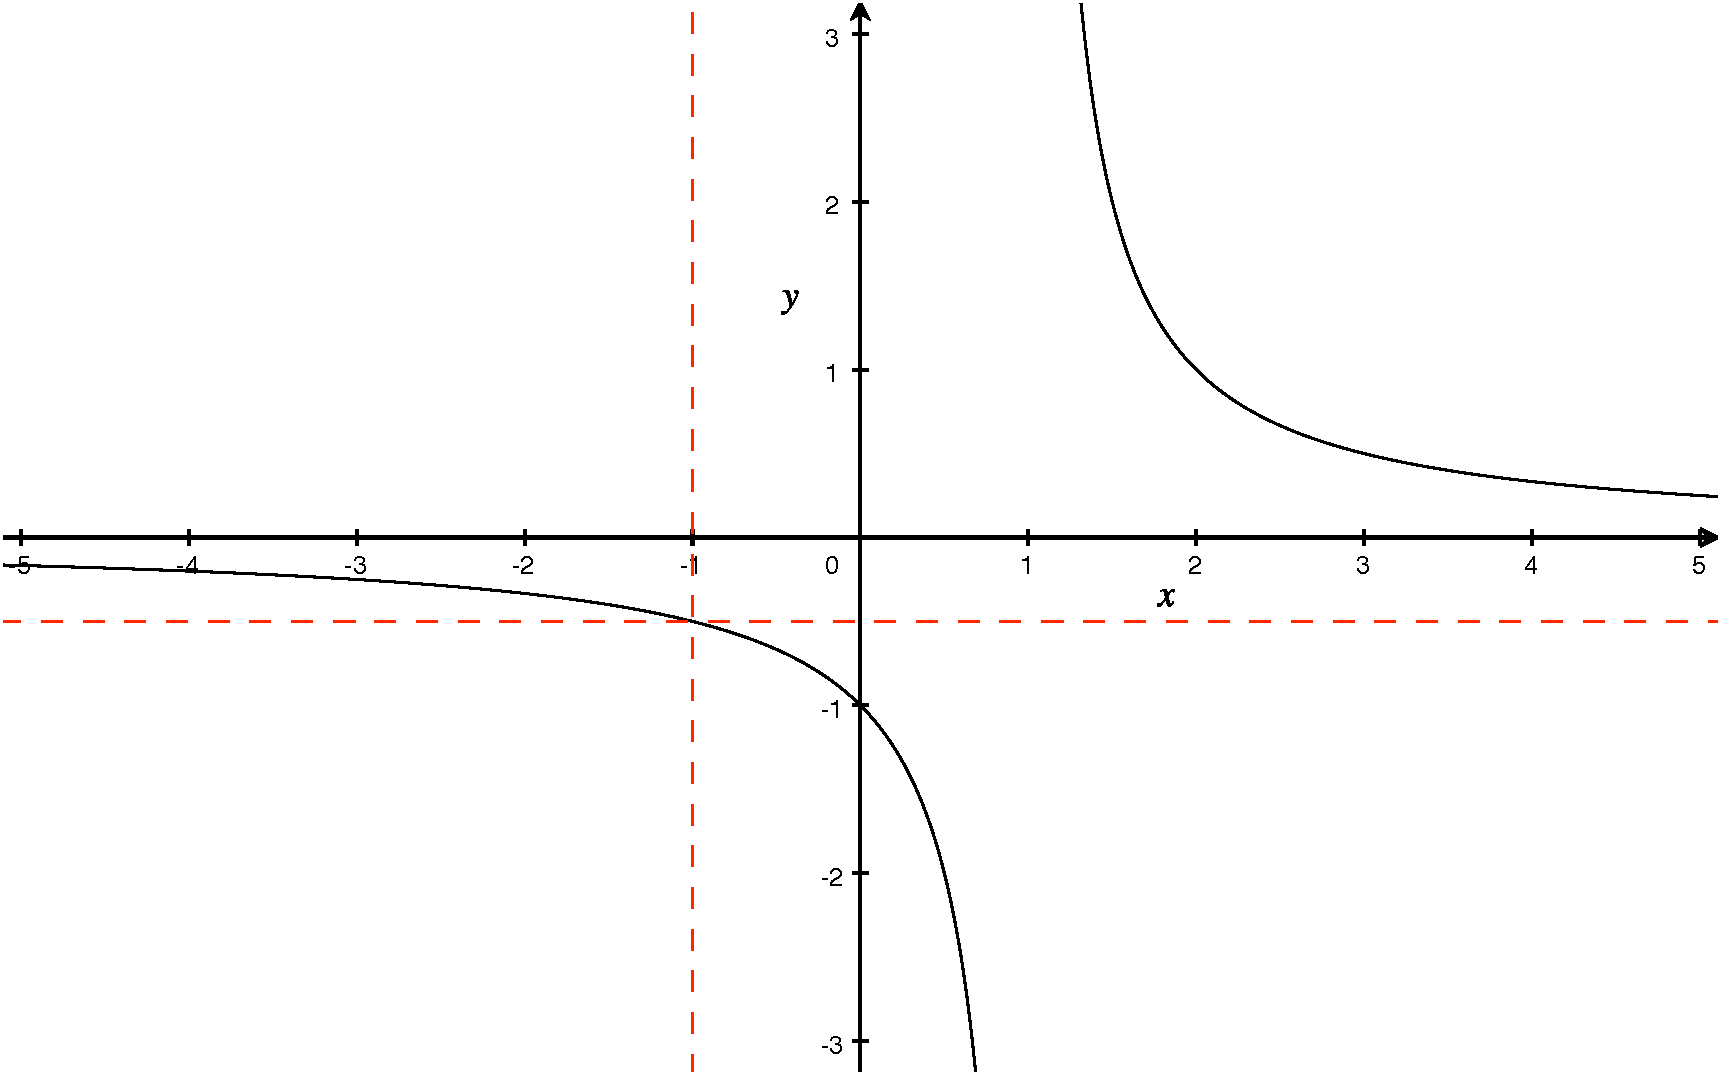
\includegraphics[width=4in]{./graphics/graph020104.pdf} 
   \caption{Graph of $\displaystyle y =  \frac{x+1}{x^2-1}$ with \emph{crosshair} at $x=-1$.}
   \label{fig:graph020104}
\end{figure}

\begin{solution}
Typically we will start with a visual  and then a sequence of numerical calculations. Here's a graph (Figure \ref{fig:graph020104}, page \pageref{fig:graph020104})


Looking at the graph you need to \emph{visualize} getting close to $x=-1$, from both left and right, to see where $\displaystyle \frac{x+1}{x^2-1}$  is going. After looking at the graph (Figure \ref{fig:graph020104}, page \pageref{fig:graph020104}), my guess is $-1/2$. I've placed a crosshair centered at $x=-1$ and you'll need to estimate what the $y$ value is. You should note that the graph is undefined at $x=-1$. So I would be visually confident to write
\[
\mathop {\lim }\limits_{x \to -1 }  \frac{x+1}{x^2-1} = - \frac{1}{2},
\]
but not certain. Again, we know where $x$ is going, but we're not totally certain where $\displaystyle \frac{x+1}{x^2-1}$ is going as $x$ gets closer to $-1$.

Now let's move on to numerical sequences. First from the right of $x=-1$.
\begin{eqnarray*}
y\left( x \right) &=& \frac{x+1}{x^2-1} = \frac{1}{x-1}, \quad x \neq -1\\
y\left( -0.9 \right) &=& - \frac{1}{1.9}\\
y\left( -0.99 \right) &=& - \frac{1}{1.99}\\
y\left( -0.999 \right) &=&- \frac{1}{1.999}
\end{eqnarray*}
Again, it looks like this sequence is going towards $-1/2$. So I write
\[
\mathop {\lim }\limits_{x \to -1^+ }  \frac{x+1}{x^2-1} = - \frac{1}{2}.
\]
Now from the left of $x=-1$.
\begin{eqnarray*}
y\left( x \right) &=& \frac{x+1}{x^2-1} = \frac{1}{x-1}, \quad x \neq -1\\
y\left( -1.1 \right) &=& - \frac{1}{2.1}\\
y\left( -1.01 \right) &=& - \frac{1}{2.01}\\
y\left( -1.001 \right) &=&- \frac{1}{2.001}
\end{eqnarray*}
Again, it looks like this sequence is going towards $-1/2$. So I write
\[
\mathop {\lim }\limits_{x \to -1^- }  \frac{x+1}{x^2-1} = - \frac{1}{2}.
\]
Everything is in agreement, so I may conclude that
\[
\mathop {\lim }\limits_{x \to -1 }  \frac{x+1}{x^2-1} = - \frac{1}{2}.
\]
For those of you interested in studying mathematics further, you should note that this is not a \emph{proof} that this limit is $-1/2$.
\end{solution}



















\subsection{Examples}




 




\begin{questions}
\question Find the limit, if it exists.
\[
\mathop {\lim }\limits_{x \to 0 }  \frac{\sqrt{x^2+4} -2}{x^2}
\]
Use values close to $x=0$, from both left and right, and use a graph.\footnote{Use: $\pm 1,\pm 0.5,\pm 0.1,\pm 0.05,\pm 0.01$.}
\begin{figure}[htbp] %  figure placement: here, top, bottom, or page
   \centering
   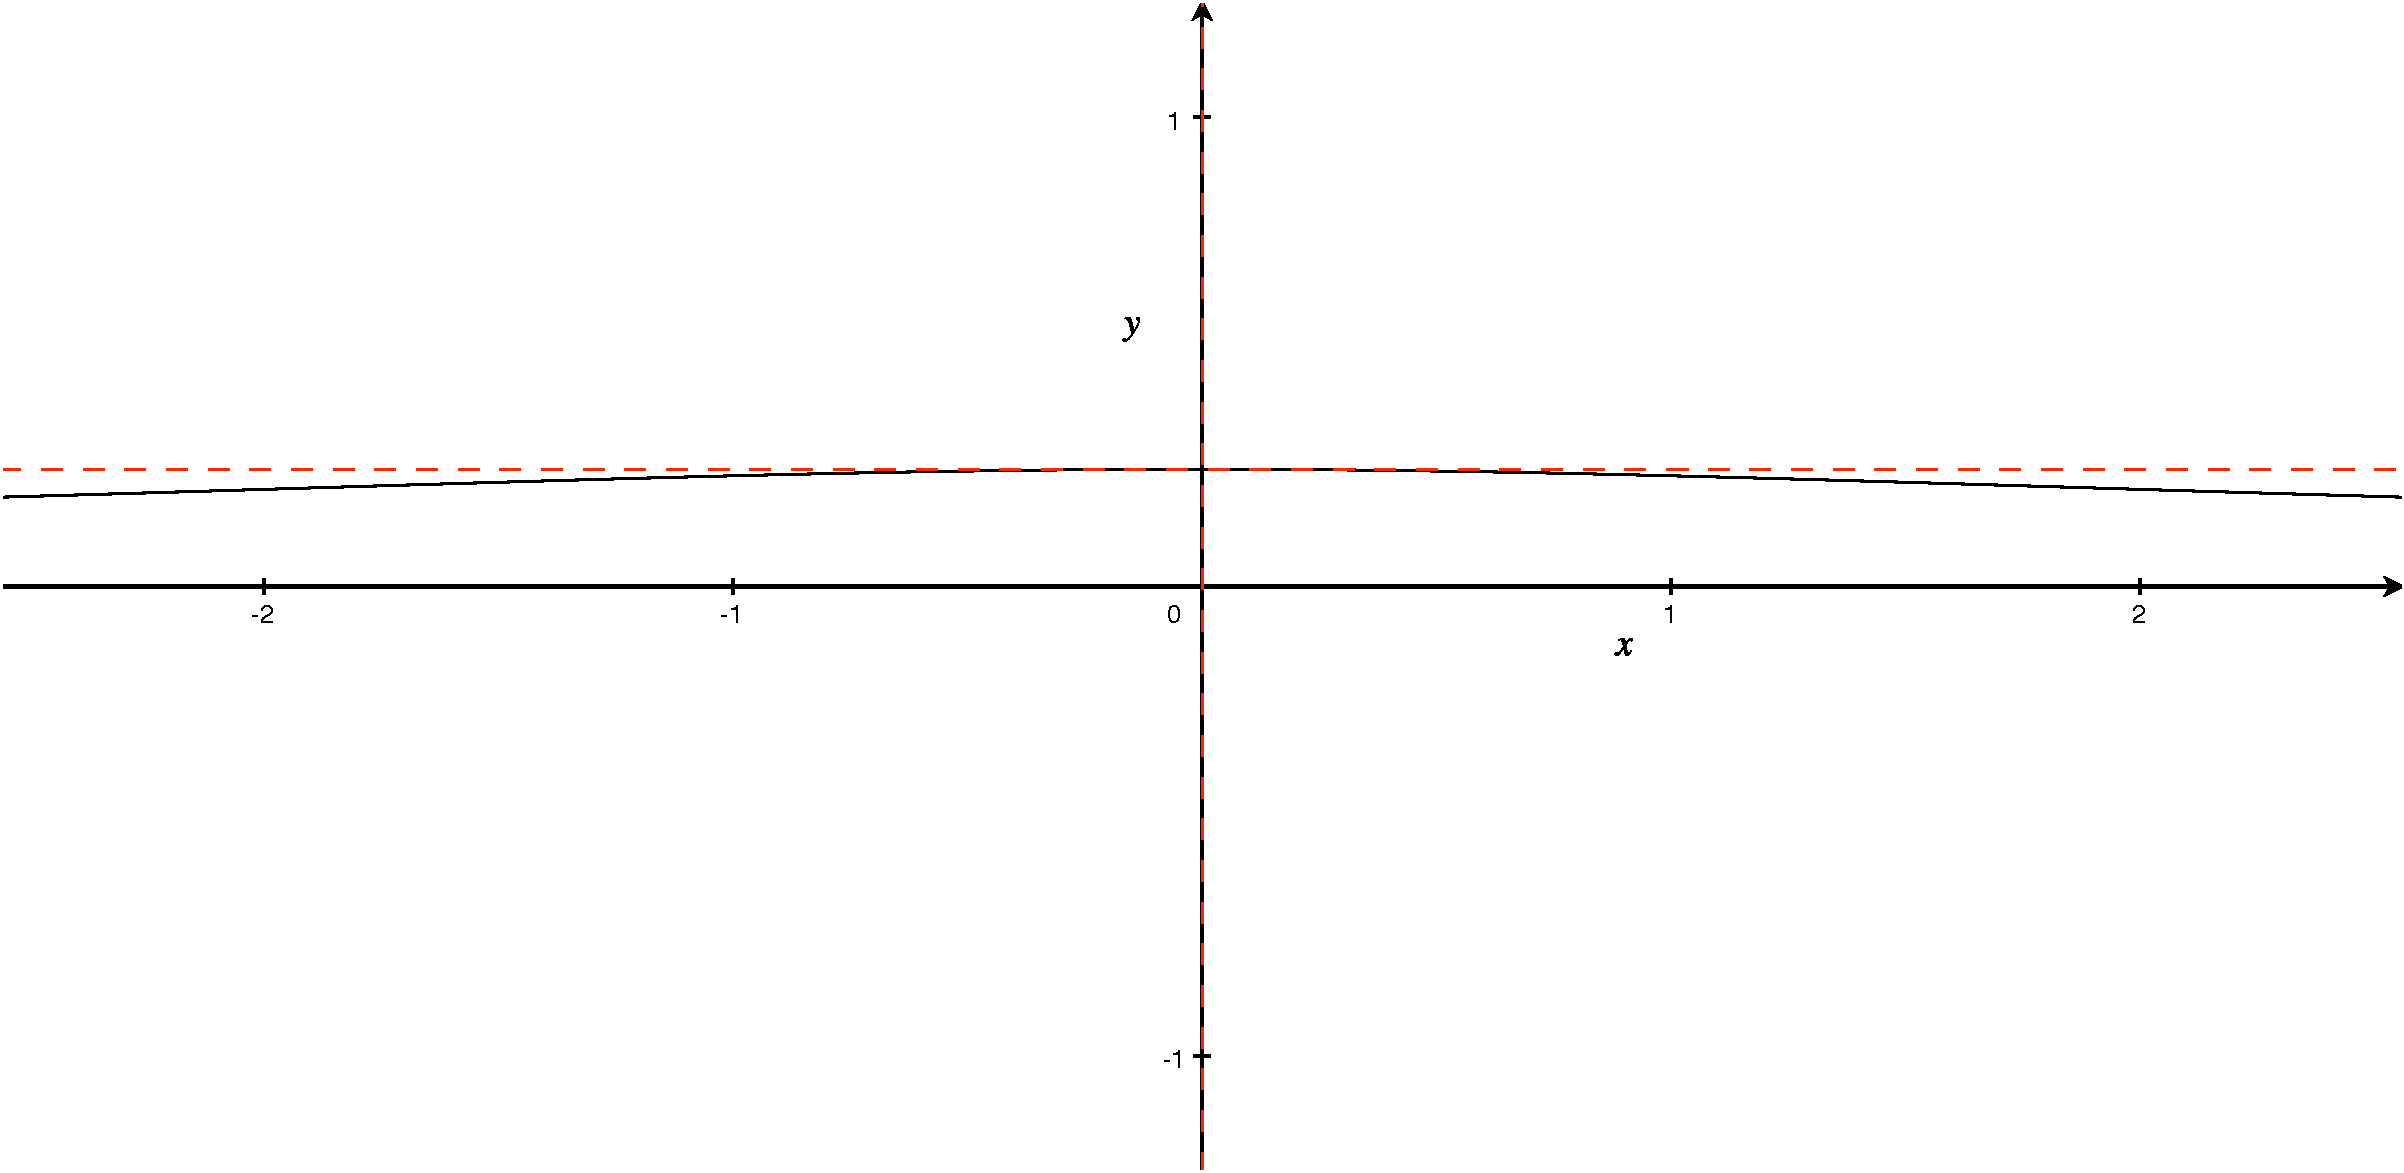
\includegraphics[width=4in]{./graphics/graph020105.pdf} 
   \caption{$\displaystyle y = \frac{\sqrt{x^2+4} -2}{x^2}$, and crosshair at $x=0$}
   \label{fig:graph020105}
\end{figure}

\begin{solution}
The graph (Figure \ref{fig:graph020105}, page \pageref{fig:graph020105}) indicates that the limit is $1/4$. Make sure you can graph this on your own!

Now let's move on to numerical sequences. First from the right of $x=0$.
\begin{eqnarray*}
y\left( x \right) &=& \frac{\sqrt{x^2+4} -2}{x^2}, \quad x \neq 0\\
y\left( 1 \right) &\approx& 0.236068\\
y\left( 0.5 \right) &\approx& 0.246211\\
y\left( 0.1 \right) &\approx& 0.249844\\
y\left( 0.05 \right) &\approx&0.249961 \\
y\left( 0.01\right) &\approx&0.249998
\end{eqnarray*}
Again, it looks like this sequence is going towards $0.25$. So I write
\[
\mathop {\lim }\limits_{x \to 0^+ }  \frac{\sqrt{x^2+4} -2}{x^2} = \frac{1}{4}.
\]
Now from the left of $x=0$.
\begin{eqnarray*}
y\left( x \right) &=& \frac{\sqrt{x^2+4} -2}{x^2}, \quad x \neq 0\\
y\left( -1 \right) &\approx& 0.236068\\
y\left( -0.5 \right) &\approx& 0.246211\\
y\left( -0. 1\right) &\approx& 0.249844\\
y\left( -0.05 \right) &\approx&0.249961 \\
y\left( -0.01 \right) &\approx&0.249998
\end{eqnarray*}
Again, it looks like this sequence is going towards $1/4$. So I write
\[
\mathop {\lim }\limits_{x \to 0^- }  \frac{\sqrt{x^2+4} -2}{x^2} = \frac{1}{4}.
\]
The graph (Figure \ref{fig:graph020105}, page \pageref{fig:graph020105})  and the table of values are in full agreement so I feel comfortable in writing
\[
\mathop {\lim }\limits_{x \to 0 }  \frac{\sqrt{x^2+4} -2}{x^2} = \frac{1}{4}.
\]
\end{solution}

\question Find the limit, if it exists.
\[
\mathop {\lim }\limits_{x \to 0 }  \cos \frac{2 \pi}{x}
\]
Use values close to $x=0$, from both left and right, and use a graph.\footnote{Use: $\pm 1,\pm 1/2,\pm 1/3,\pm 1/4,\pm 1/6$.}

\begin{figure}[htbp] %  figure placement: here, top, bottom, or page
   \centering
   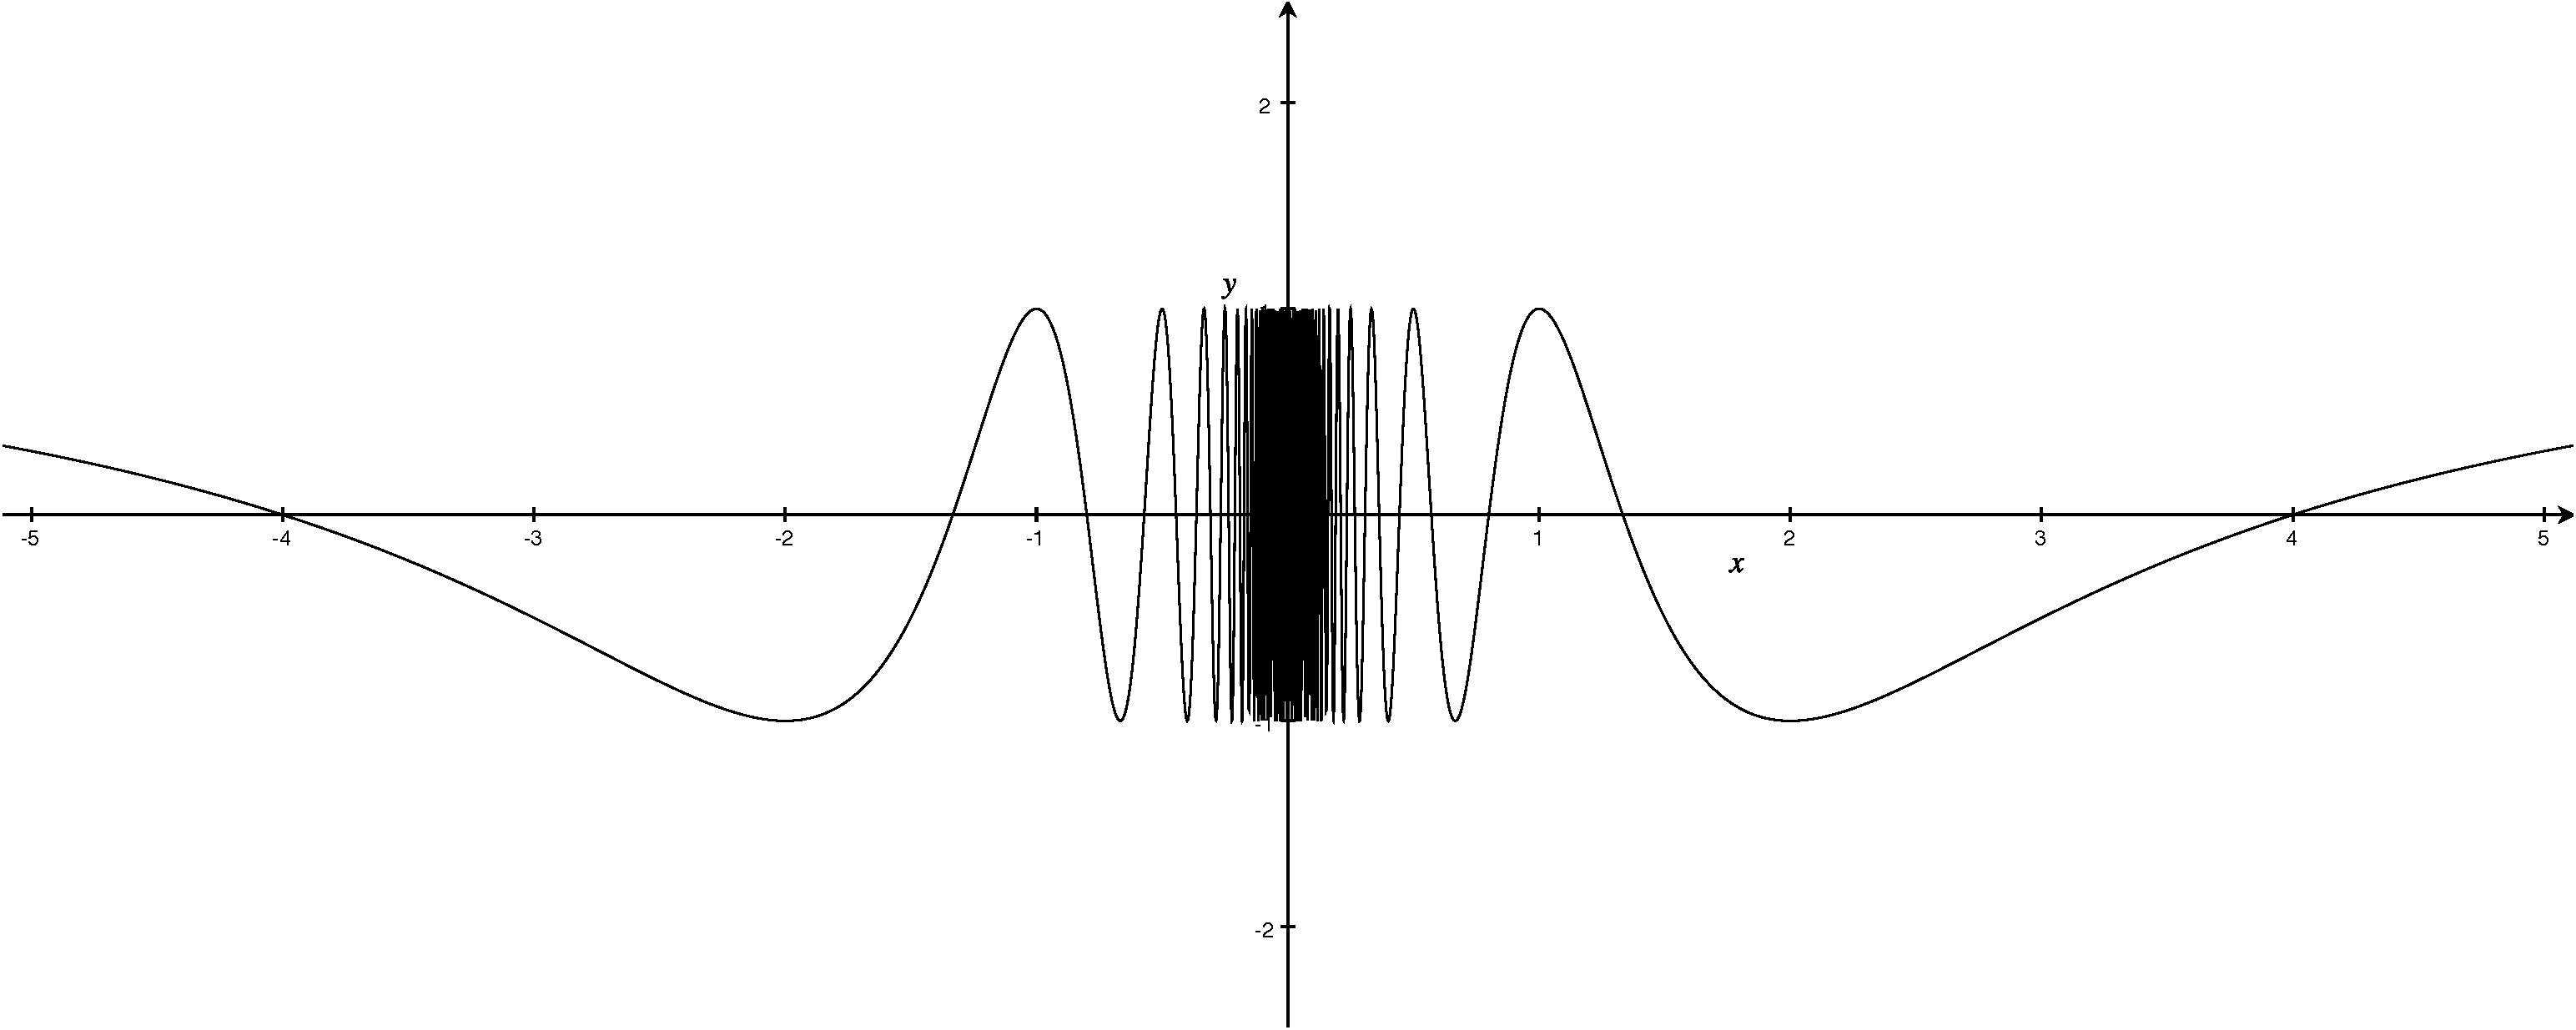
\includegraphics[width=4in]{./graphics/graph020106.pdf} 
   \caption{$\displaystyle y = \cos \frac{2 \pi}{x}$}
   \label{fig:graph020106}
\end{figure}

\begin{solution}
The graph (Figure \ref{fig:graph020106}, page \pageref{fig:graph020106}) indicates that the limit is does not exist (DNE) because it does not go towards a single number. Make sure you can graph this on your own!

Now let's move on to numerical sequences. First from the right of $x=0$.
\begin{eqnarray*}
y\left( x \right) &=& \cos \frac{2 \pi}{x}, \quad x \neq 0\\
y\left( 1 \right) &=& 1\\
y\left( 1/2 \right) &=& 1\\
y\left( 1/3 \right) &=& 1\\
y\left( 1/4 \right) &=&1\\
y\left( 1/6 \right) &=&1
\end{eqnarray*}
Again, it looks like this sequence is going towards $1$. So I write
\[
\mathop {\lim }\limits_{x \to 0^+ }  \cos \frac{2 \pi}{x}  = 1.\quad \mbox{This is actually \emph{wrong}!}
\]
Now from the left of $x=0$.
\begin{eqnarray*}
y\left( x \right) &=& \cos \frac{2 \pi}{x}, \quad x \neq 0\\
y\left( -1 \right) &=& 1\\
y\left( -1/2 \right) &=& 1\\
y\left( -1/3 \right) &=& 1\\
y\left( -1/4 \right) &=&1 \\
y\left( -1/6 \right) &=&1
\end{eqnarray*}



Again, it looks like this sequence is going towards $1$. So I write
\[
\mathop {\lim }\limits_{x \to 0^- }  \cos \frac{2 \pi}{x} = 1. \quad \mbox{This is actually \emph{wrong}!}
\]


\begin{center}
\textbf{Don't be fooled!}
\end{center}


The graph (Figure \ref{fig:graph020106}, page \pageref{fig:graph020106})  and the table of values are in disagreement! Yes, the values were chosen to illustrate that picking \emph{easy} values may in fact lead to a \textbf{wrong} answer. Initially it is particularly important that you can both graph and use tables to feel your way through limit problems, It requires work, but once you master the use of your calculators you should be able to do this quickly.



The \textbf{correct} answer is
\[
\mathop {\lim }\limits_{x \to 0 }  \cos \frac{2 \pi}{x} = DNE.
\]
\end{solution}







\question Find the limit, if it exists.
\[
\mathop {\lim }\limits_{x \to 0 } \frac{\tan x - x}{x^3}
\]
Use values close to $x=0$, from both left and right, and use a graph.\footnote{Use: $\pm 1,\pm 0.5,\pm 0.1,\pm 0.05,\pm 0.01, \pm 0.0005$.}
\begin{figure}[htbp] %  figure placement: here, top, bottom, or page
   \centering
   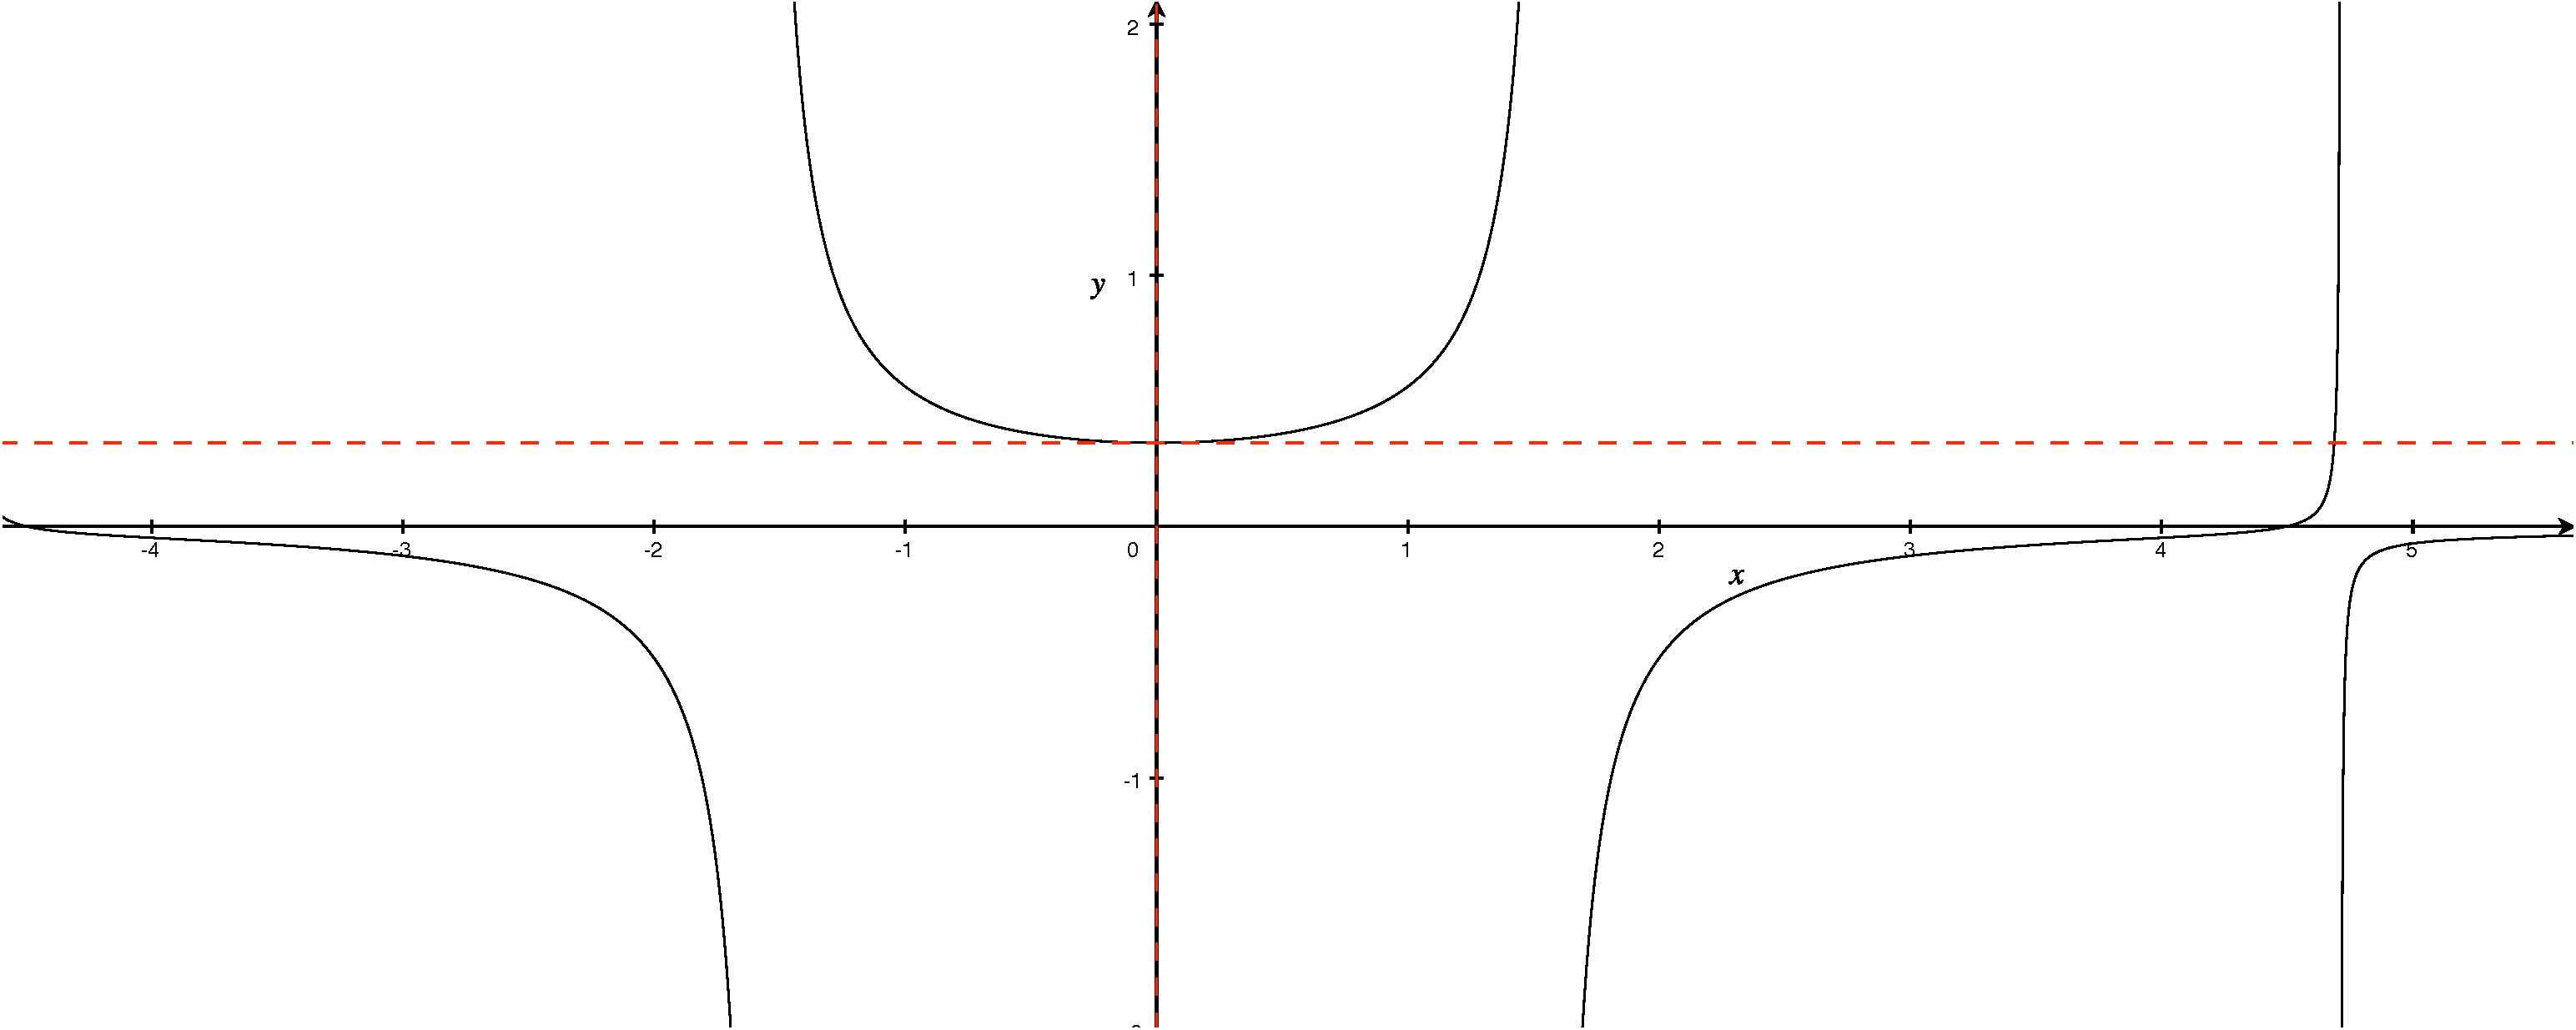
\includegraphics[width=4in]{./graphics/graph020107.pdf} 
   \caption{$\displaystyle y = \frac{\tan x - x}{x^3}$, and crosshair at $x=0$}
   \label{fig:graph020107}
\end{figure}
\begin{solution}
The graph (Figure \ref{fig:graph020107}, page \pageref{fig:graph020107}) indicates that the limit is $1/3$. Make sure you can graph this on your own!


I am not providing tables here, but you should be capable of doing this on your own now. Be aware that you will need to be able to do this on assignments and exams!
\[
\mathop {\lim }\limits_{x \to 0 } \frac{\tan x - x}{x^3} =\frac{1}{3}
\]
\end{solution}




\question Find the limit, if it exists.\footnote{Exists means that the limit is a finite number. However, if the number gets ``big'' without bound we use this symbol $\infty$ indicating infinity. You should specify, using $\pm$, what direction the infinity is going in.}
\[
\mathop {\lim }\limits_{x \to 2^+ } \frac{1}{2-x}
\]
Use values close to $x=2$, from the right.
\begin{figure}[htbp] %  figure placement: here, top, bottom, or page
   \centering
   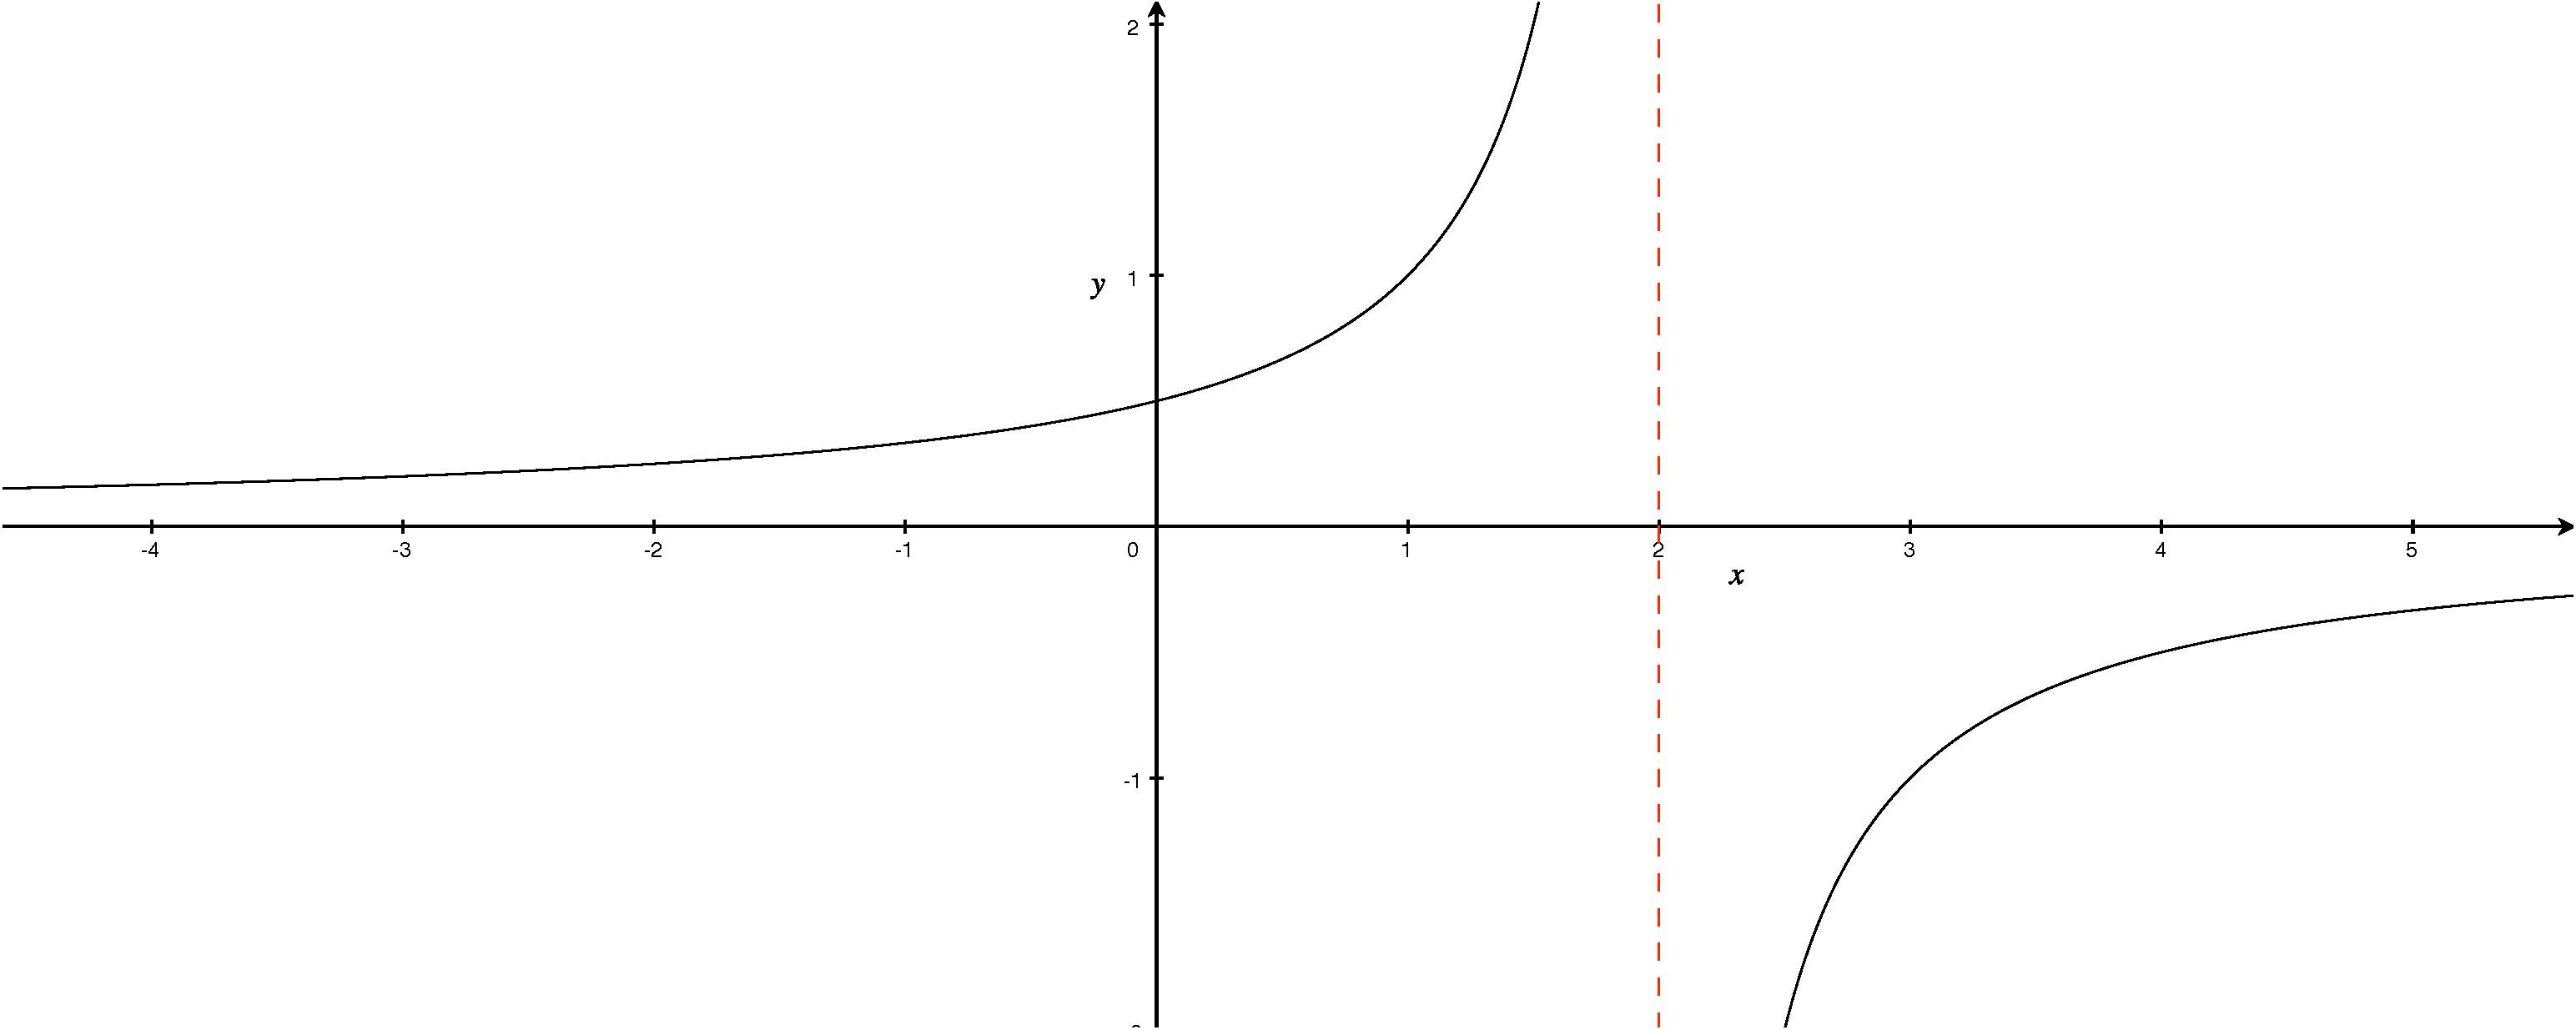
\includegraphics[width=4in]{./graphics/graph020108.pdf} 
   \caption{$\displaystyle y = \frac{1}{2-x}$, and asymptote at $x=2$}
   \label{fig:graph020108}
\end{figure}
\begin{solution}
The graph (Figure \ref{fig:graph020108}, page \pageref{fig:graph020108}) indicates that the limit is infinite in the negative direction, and we indicate this using $- \infty$. Make sure you can graph this on your own!

Again, you should be able to create a reasonable table by now!
\[
\mathop {\lim }\limits_{x \to 2^+ } \frac{1}{2-x} = -\infty
\]
\end{solution}


\question Find the limit, if it exists.
\[
\mathop {\lim }\limits_{x \to 2^- } \frac{1}{2-x}
\]
Use values close to $x=2$, from the left.
\begin{figure}[htbp] %  figure placement: here, top, bottom, or page
   \centering
   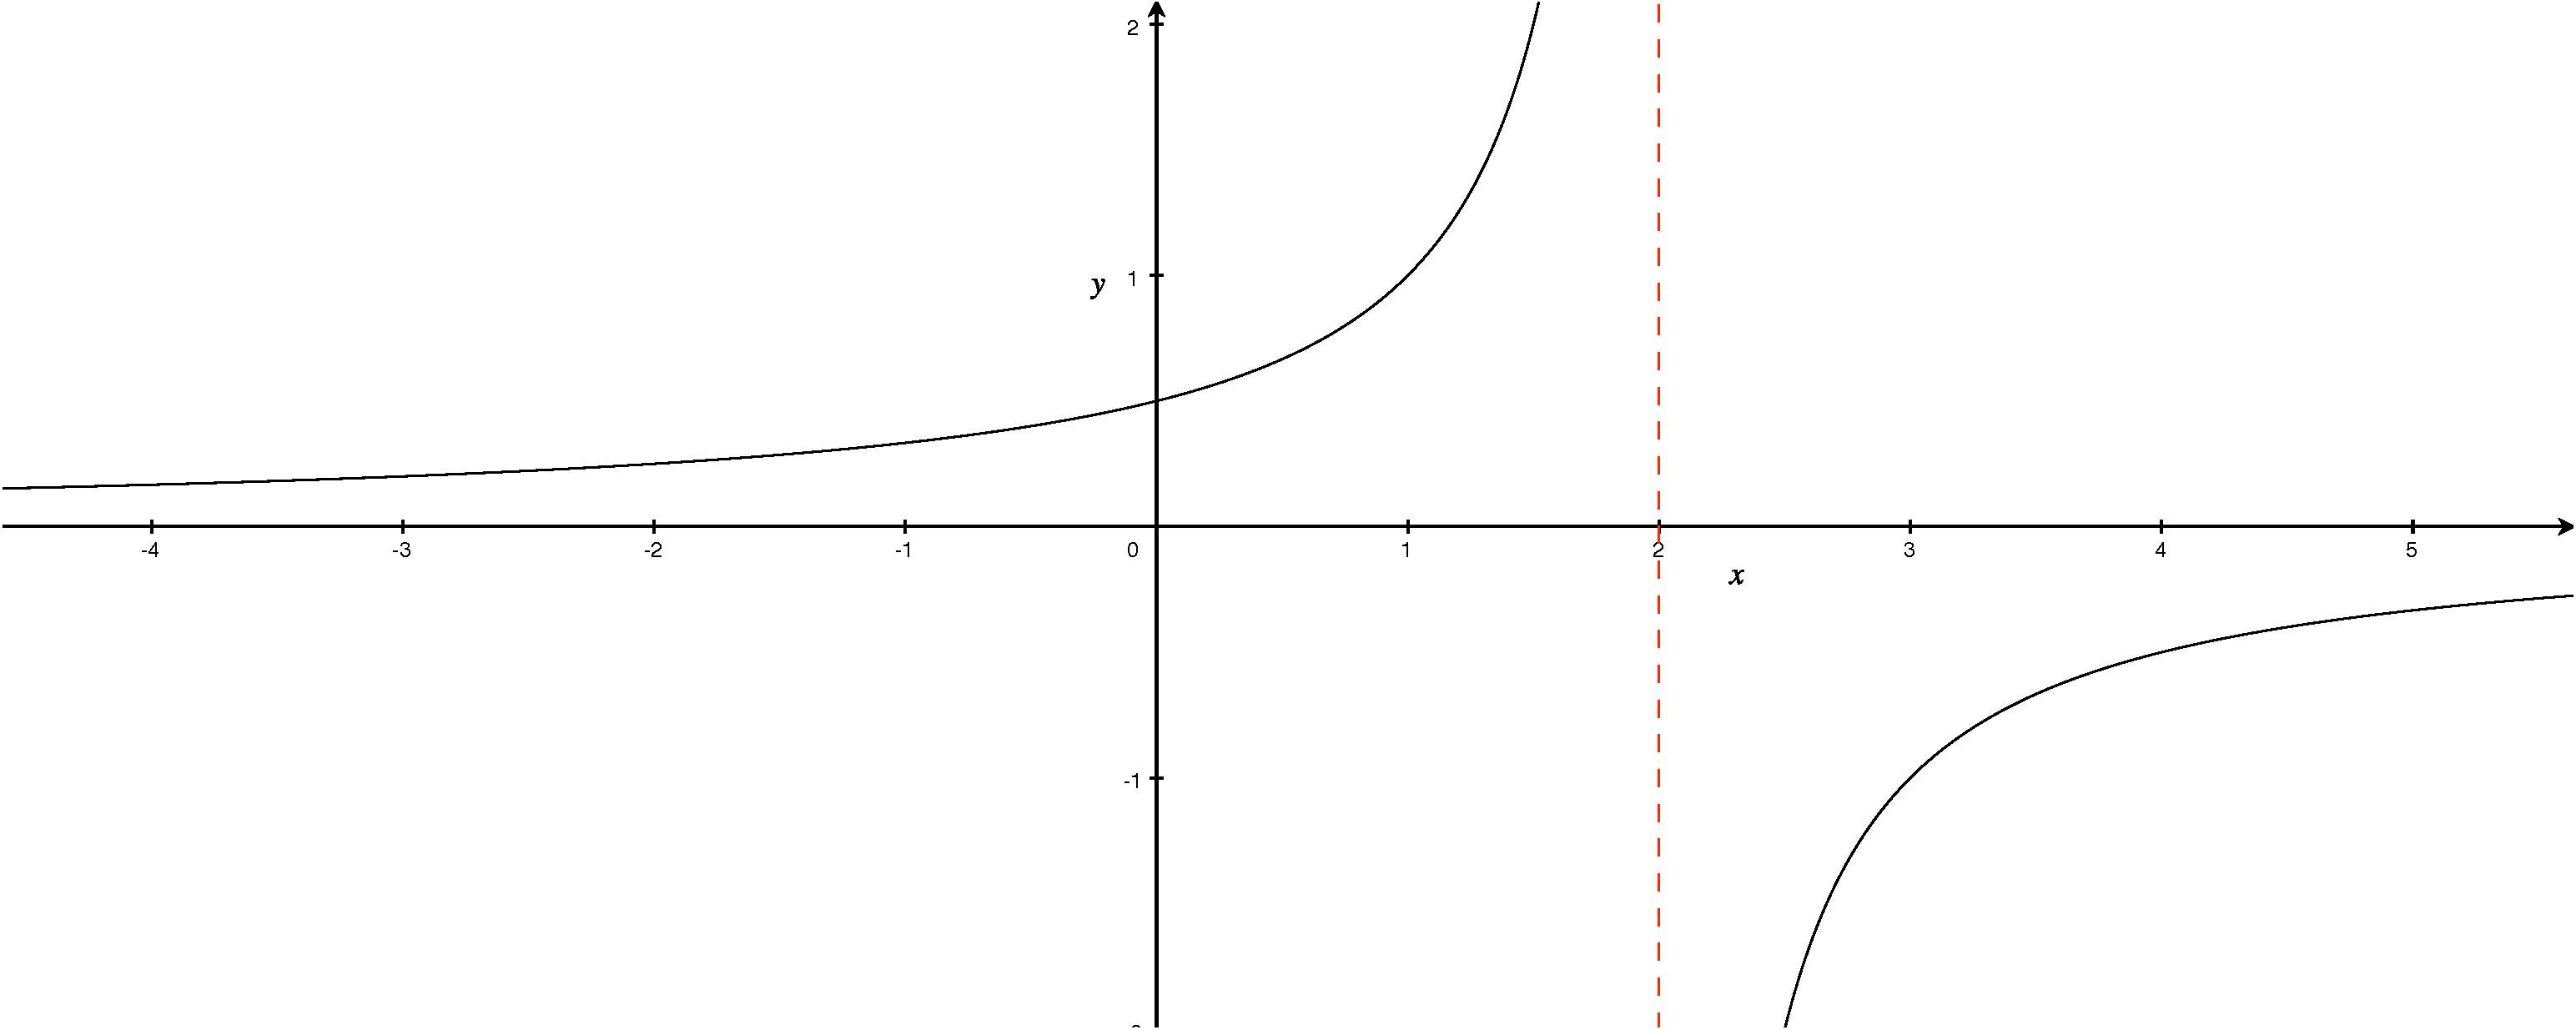
\includegraphics[width=4in]{./graphics/graph020108.pdf} 
   \caption{$\displaystyle y = \frac{1}{2-x}$, and asymptote at $x=2$}
   \label{fig:graph020109}
\end{figure}
\begin{solution}
The graph (Figure \ref{fig:graph020109}, page \pageref{fig:graph020109}) indicates that the limit is infinite in the positive direction, and we indicate this using $ \infty$. Make sure you can graph this on your own!

Again, you should be able to create a reasonable table by now!
\[
\mathop {\lim }\limits_{x \to 2^- } \frac{1}{2-x} = \infty
\]
\end{solution}


\question Find the limit, if it exists.
\[
\mathop {\lim }\limits_{x \to 2 } \frac{1}{2-x}
\]
\begin{solution}
\[
\mathop {\lim }\limits_{x \to 2 } \frac{1}{2-x} = DNE
\]
\end{solution}



\question Without using a graph or tables, evaluate each of the following by trying to \emph{visualize} in your head what the limit is.\footnote{This may involve simple mental arithmetic as well.}
\begin{parts}
\part Find the limit, if it exists.
\[
\lim_{x \to 5 } 3x-2
\]
\begin{solution}
It's a line and you should be able to reason that the limit exists.
\[
\lim_{x \to 5 } 3x-2 = 13
\]
\end{solution}
\part Find the limit, if it exists.
\[
\lim_{x \to 1 } x^2-2x+3
\]
\begin{solution}
It's a parabola and you should be able to reason that the limit exists.
\[
\lim_{x \to 1 } x^2-2x+3 = 2
\]
\end{solution}
\part Find the limit, if it exists.
\[
\lim_{x \to -1 } \pi
\]
\begin{solution}
It's a horizontal line and you should be able to reason that the limit exists.
\[
\lim_{x \to -1} \pi = \pi
\]
\end{solution}
\end{parts}

\question Given the following graph (Figure \ref{fig:227_limit}, page \pageref{fig:227_limit}) determine each of the limits.
\begin{figure}[htbp] %  figure placement: here, top, bottom, or page
   \centering
   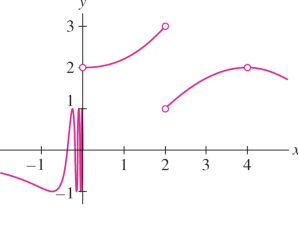
\includegraphics[width=4in]{./graphics/227_limit.pdf} 
   \caption{Partial graph of $f\left(x\right)$.}
   \label{fig:227_limit}
\end{figure}
\begin{parts}
\part
\[
\lim_{x \to 0^-} f\left(x\right) =
\]
\begin{solution}
We will discuss this in class.
\end{solution}
\part
\[
\lim_{x \to 0^+} f\left(x\right) =
\]
\begin{solution}
We will discuss this in class.
\end{solution}
\part
\[
\lim_{x \to 0} f\left(x\right) =
\]
\begin{solution}
We will discuss this in class.
\end{solution}
\part
\[
\lim_{x \to 2^-} f\left(x\right) =
\]
\begin{solution}
We will discuss this in class.
\end{solution}
\part
\[
\lim_{x \to 2^+} f\left(x\right) =
\]
\begin{solution}
We will discuss this in class.
\end{solution}
\part
\[
\lim_{x \to 2} f\left(x\right) =
\]
\begin{solution}
We will discuss this in class.
\end{solution}
\part
\[
\lim_{x \to 4^-} f\left(x\right) =
\]
\begin{solution}
We will discuss this in class.
\end{solution}
\part
\[
\lim_{x \to 4^+} f\left(x\right) =
\]
\begin{solution}
We will discuss this in class.
\end{solution}
\part
\[
\lim_{x \to 4} f\left(x\right) =
\]
\begin{solution}
We will discuss this in class.
\end{solution}
\end{parts}

\end{questions}
\subsection{Assignment}
You should read \S  2.2 and do the WebAssign assignment mth.121.02.02.
\vfill
\pagebreak
%*-*-*-*-*-*-*-*-*-*-*-*-*-*-*-*-*-*-*-*-*-*-*-*-*-*-*-*-*-*-*-*-*-*-*-*-*-*-*-*-*-*-*-*-*-*-*-*-*-*-*-*-*-*-*-*-*-*-*-*-*-*-*-*-*-*-*-*-*-*-*-*-*-*-*-*-*-*-*-*-*-*-*-*-

\begin{teacher}
\subsection{Assessments}
The following questions are related to the WebAssign assignments and may be used to assess students' ability. Please do not share any of these questions with students.
\begin{questions}	
\question 	%RogaCalcET2 2.2.001	WA-1701016

Fill in the table below, where
\[
f\left(x\right) = \frac{ x^3 - 27}{x^2 - 9}.
\]
(Round your answers to three decimal places.)
\begin{parts}
\part $f\left(3.0020\right) \approx$
\begin{solution}
\end{solution}
\part $f\left(3.0010\right) \approx$
\begin{solution}
\end{solution}
\part $f\left(3.0005\right) \approx$
\begin{solution}
\end{solution}
\part $f\left(3.0001\right) \approx$
\begin{solution}
\end{solution}
\part $f\left(2.9980\right) \approx$
\begin{solution}
\end{solution}
\part $f\left(2.9990\right) \approx$
\begin{solution}
\end{solution}
\part $f\left(2.9995\right) \approx$
\begin{solution}
\end{solution}
\part $f\left(2.9999\right) \approx$
\begin{solution}
\end{solution}
\part Guess the value of
\[
\lim_{x \to 3} f \left( x \right) =
\]
\begin{solution}
\end{solution}
\end{parts}


\question 	%RogaCalcET2 2.2.004	WA-1700994

Fill in the table below, where 
\[
f\left(x\right) = x \ln 9x.
\]
(Round your answers to three decimal places.)

\begin{parts}
\part $f\left(1.0000\right) \approx$
\begin{solution}
\end{solution}
\part $f\left(0.5000\right) \approx$
\begin{solution}
\end{solution}
\part $f\left(0.1000\right) \approx$
\begin{solution}
\end{solution}
\part $f\left(0.0500\right) \approx$
\begin{solution}
\end{solution}
\part $f\left(0.0100\right) \approx$
\begin{solution}
\end{solution}
\part $f\left(0.0050\right) \approx$
\begin{solution}
\end{solution}
\part $f\left(0.0010\right) \approx$
\begin{solution}
\end{solution}
\part $f\left(0.0005\right) \approx$
\begin{solution}
\end{solution}
\part Guess the value of
\[
\lim_{x \to 0^+} f \left( x \right) =
\]
\begin{solution}
\end{solution}
\end{parts}


\question 	%RogaCalcET2 2.2.008	WA-1701035

Evaluate the limit.
\[
\lim_{x \to 4.7} \sqrt{7}
\]
\begin{solution}
\end{solution}

\question 	%RogaCalcET2 2.2.009	WA-1718965

Evaluate the limit.
\[
\lim_{x \to 2} 3x
\]
\begin{solution}
\end{solution}

\question 	%RogaCalcET2 2.2.011	WA-1718980

Evaluate the limit.
\[
\lim_{x \to 6} \left( 3x+8\right)
\]
\begin{solution}
\end{solution}

\question 	%RogaCalcET2 2.2.012	WA-1718970

Evaluate the limit.
\[
\lim_{x \to 4} \left( 5x - 8\right)
\]
\begin{solution}
\end{solution}

\question 	%RogaCalcET2 2.2.014	WA-1718978

Evaluate the limit.
\[
\lim_{x \to 3} \left( 3x^2 - 5 \right)
\]
\begin{solution}
\end{solution}

\question 	%RogaCalcET2 2.2.017.T	WA-1689395

Estimate the limit numerically or state that the limit doesn't exist. (Round your answer to four decimal places. If an answer does not exist, enter DNE.)
\[
\lim_{x \to 9} \frac{\sqrt{x} -3}{x-9}
\]
\begin{solution}
\end{solution}

\question 	%RogaCalcET2 2.2.018	WA-1725660

Evaluate the limit numerically or state that the limit doesn't exist. (Round your answer to three decimal places. If you need to use  $\infty$ or $-\infty$, enter INFINITY or –INFINITY, respectively. If an answer does not exist, enter DNE.)
\[
\lim_{x \to -3} \frac{2x^2-18}{x+3}
\]
\begin{solution}
\end{solution}

\question 	%RogaCalcET2 2.2.020	WA-1701062

Evaluate the limit numerically or state that the limit doesn't exist. (Round your answer to three decimal places. If an answer does not exist, enter DNE.)
\[
\lim_{x \to 7} \frac{x^3-6x^2-49}{x^2-8x+7}
\]
\begin{solution}
\end{solution}

\question 	%RogaCalcET2 2.2.021	WA-1701028

Evaluate the limit numerically or state that the limit doesn't exist. (Round your answer to three decimal places. If an answer does not exist, enter DNE.)
\[
\lim_{x \to 0} \frac{\sin 10x}{x}
\]
\begin{solution}
\end{solution}

\question 	%RogaCalcET2 2.2.023	WA-1701046

Evaluate the limit numerically or state that the limit doesn't exist. (Round your answer to three decimal places. If an answer does not exist, enter DNE.)
\[
\lim_{\theta \to 0} \frac{3\cos \theta - 3}{2\theta}
\]
\begin{solution}
\end{solution}

\question 	%RogaCalcET2 2.2.026	WA-1718991

Evaluate the limit numerically or state that the limit doesn't exist. (Round your answer to three decimal places. If you need to use $\infty$ or $-\infty$, enter INFINITY or –INFINITY, respectively. If an answer does not exist, enter DNE.)
\[
\lim_{x\to 7^-} \frac{2-x}{x-7}
\]
\begin{solution}
\end{solution}

\question 	%RogaCalcET2 2.2.028	WA-1700957

Evaluate the limit numerically or state that the limit doesn't exist. (Round your answer to three decimal places. If an answer does not exist, enter DNE.)
\[
\lim_{h\to 0} \frac{7^h-1}{h}
\]
\begin{solution}
\end{solution}

\question 	%RogaCalcET2 2.2.032	WA-1700990

Evaluate the limit numerically or state that the limit doesn't exist. (Round your answer to three decimal places. If an answer does not exist, enter DNE.)\footnote{$\sec^{-1} x = \arccos x^{-1}$}
\[
\lim_{x\to 1^+} \frac{\sec^{-1} x}{\sqrt{x^5-1}}
\]
\begin{solution}
\end{solution}

\question 	%RogaCalcET2 2.2.034	WA-1689420

Estimate the limit numerically or state that the limit does not exist. (Round your answer to two decimal places. If an answer does not exist, enter DNE.)
\[
\lim_{r\to 0} \left( 1 + r \right)^{3/r}
\]
\begin{solution}
\end{solution}


\question 	%RogaCalcET2 2.2.038	WA-1725329

Determine the one-sided limit of the function $y\left(x\right)$ in the figure below at the given point. (If an answer does not exist, enter DNE.)
\[
\lim_{x \to 4^-} y\left(x\right)
\]
\begin{figure}[htbp] %  figure placement: here, top, bottom, or page
   \centering
   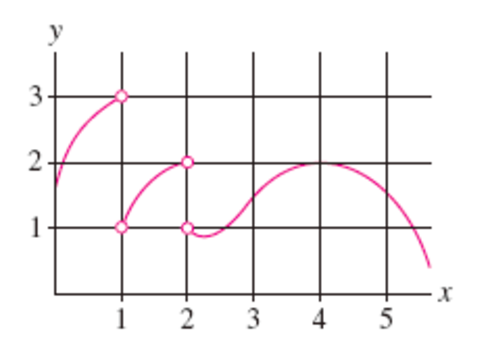
\includegraphics[width=3in]{./graphics/1725329.pdf} 
   \caption{WA-1725329}
   \label{fig:1725329}
\end{figure}
\begin{solution}
\end{solution}

\question 	%RogaCalcET2 2.2.053	WA-1722946

Determine the one-sided limit of the function $y\left(x\right)$ in the figure below at the given point. (If you need to use $\infty$ or $-\infty$, enter INFINITY or –INFINITY, respectively. If an answer does not exist, enter DNE.)
\[
\lim_{x \to 5^+} y\left(x\right)
\]
\begin{figure}[htbp] %  figure placement: here, top, bottom, or page
   \centering
   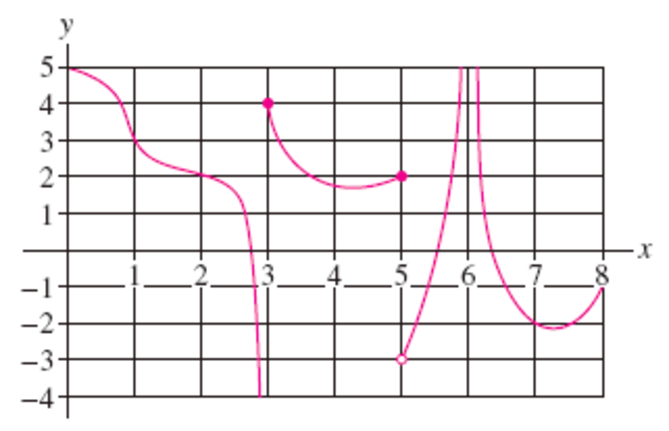
\includegraphics[width=3in]{./graphics/1722946.pdf} 
   \caption{WA-1722946}
   \label{fig:1722946}
\end{figure}
\begin{solution}
\end{solution}

\question 	%RogaCalcET2 2.2.055	WA-1701008

Plot the function and use the graph to estimate the value of the limit. (Round your answer to three decimal places.)
\[
\lim_{x \to 0} \frac{\sin 8x}{\sin 4x}
\]
\begin{solution}
\end{solution}



\question 	%RogaCalcET2 2.2.056	WA-1725317

Plot the function and use the graph to estimate the value of the limit. (Round your answer to two decimal places.)
\[
\lim_{x \to 0} \frac{7^x - 1}{4^x - 1}
\]
\begin{solution}
\end{solution}


\end{questions}
\end{teacher}






\vfill
\pagebreak





%*-*-*-*-*-*-*-*-*-*-*-*-*-*-*-*-*-*-*-*-*-*-*-*-*-*-*-*-*-*-*-*-*-*-*-*-*-*-*-*-*-*-*-*-*-*-*-*-*-*-*-*-*-*-*-*-*-*-*-*-*-*-*-*-*-*-*-*-*-*-*-*-*-*-*-*-*-*-*-*-*-*-*-*-
\section{mth.121.02.03}
\subsection{Calculating Limits}


\subsubsection{Limit Laws}

Suppose that $c$ is a constant and the limits
\[
\mathop {\lim }\limits_{x \to a }  f \left( x \right) \qquad \mbox \qquad \mathop {\lim }\limits_{x \to a }  g \left( x \right)
\]
exist. Then
\begin{eqnarray*}
\mathop {\lim }\limits_{x \to a }  \left[ f \left( x \right) +   g \left( x \right) \right] &=& \mathop {\lim }\limits_{x \to a }  f \left( x \right) + \mathop {\lim }\limits_{x \to a }  g \left( x \right)\\
\mathop {\lim }\limits_{x \to a }  \left[ f \left( x \right) -   g \left( x \right) \right] &=& \mathop {\lim }\limits_{x \to a }  f \left( x \right) - \mathop {\lim }\limits_{x \to a }  g \left( x \right)\\
\mathop {\lim }\limits_{x \to a }  \left[ c \cdot f \left( x \right)  \right] &=& c \cdot \mathop  {\lim }\limits_{x \to a }  f \left( x \right)\\
\mathop {\lim }\limits_{x \to a }  \left[ f \left( x \right)  \cdot  g \left( x \right) \right] &=& \mathop {\lim }\limits_{x \to a }  f \left( x \right) \cdot \mathop {\lim }\limits_{x \to a }   g \left( x \right)\\
\mathop {\lim }\limits_{x \to a }  \left[ \frac{f \left( x \right)}{g \left( x \right)} \right] &=& \frac{\mathop {\lim }\limits_{x \to a }  f \left( x \right) }{ \mathop {\lim }\limits_{x \to a }   g \left( x \right)} \quad \mbox{if} \quad \mathop {\lim }\limits_{x \to a }  g \left( x \right) \neq 0
\end{eqnarray*}
These are the basic limit laws, but if you look in the book you'll see more. Bottom line, you'll need to carefully think about getting close to a number without actually touching it. Furthermore, any given number can be approached from two sides---and you must think through this carefully. Here are some additional, and useful, limit laws.
\begin{eqnarray*}
\mathop {\lim }\limits_{x \to a }  \left[ f \left( x \right) \right]^n &=& \left[ \mathop {\lim }\limits_{x \to a }   f \left( x \right) \right]^n \qquad n \in \mathbb{Z}^+\\
\mathop {\lim }\limits_{x \to a }  c &=& c\\
\mathop {\lim }\limits_{x \to a }  x &=& a\\
\mathop {\lim }\limits_{x \to a }  x^n &=& a^n \qquad n \in \mathbb{Z}^+ \\
\mathop {\lim }\limits_{x \to a }  \sqrt[n]{x} &=& \sqrt[n]{a} \qquad n \in \mathbb{Z}^+ \quad \mbox{If $n$ is even, we must have $a>0$.}\\
\mathop {\lim }\limits_{x \to a }  \sqrt[n]{f\left(x\right)} &=& \sqrt[n]{\mathop {\lim }\limits_{x \to a }  f\left(x\right)} \qquad n \in \mathbb{Z}^+ \quad \mbox{If $n$ is even, we must have $\mathop {\lim }\limits_{x \to a }  f\left(x\right)>0$.}\\
\end{eqnarray*}
Certainly, there are other useful limit laws. As we all know, laws can be quite confusing, and I am not trying to suggest that these laws are easily understood, let-alone provable. Again, using your head is important, and constantly ask yourself what's happening to the function as $x$ gets close to $a$ (don't touch $a$). Look from both the left and right---just like you're crossing the street! Furthermore, the information you receive from the left and right better agree. Understanding this takes time, and you may on occasion have to resort to tables and/or graphs to clarify your beliefs.



\subsection{Examples}
\begin{questions}
\question Evaluate the limit using the basic limit laws.
\[
\lim_{x \to 1} \frac{1}{x^2}
\]
\begin{solution}
This will be discussed in class.
\end{solution}

\question Evaluate the limit using the basic limit laws.
\[
\lim_{x \to 8} 3x^{2/3}-16x^{-1}
\]
\begin{solution}
This will be discussed in class.
\end{solution}


\question Evaluate the limit using the basic limit laws.
\[
\lim_{x \to 9} \frac{\sqrt{x}}{x-2}
\]
\begin{solution}
This will be discussed in class.
\end{solution}


\question Evaluate the limit using the basic limit laws.
\[
\lim_{x \to 1/3} \left(18x^2-4\right)^4
\]
\begin{solution}
This will be discussed in class.
\end{solution}


\question Can the quotient law be applied to
\[
\lim_{x \to 0} \frac{\sin x}{x}?
\]
Explain.
\begin{solution}
This will be discussed in class.
\end{solution}


\question Evaluate using a graph and/or table of values.
\[
\lim_{x \to 0} \frac{\sin x}{x}
\]
\begin{solution}
This will be discussed in class.
\end{solution}

\end{questions}










\subsection{Assignment}
You should read \S  2.3 and do the WebAssign assignment mth.121.02.03.
\vfill
\pagebreak


\begin{teacher}
\subsection{Assessments}
The following questions are related to the WebAssign assignments and may be used to assess students' ability. Please do not share any of these questions with students.
\begin{questions}	
\question 	%RogaCalcET2 2.3.005.T	WA-1689433

Evaluate the limit using the Limit Laws.
\[
\lim_{t \to 3} 2t^{-1}
\]
\begin{solution}
\end{solution}

\question 	%RogaCalcET2 2.3.009	WA-1700996

Evaluate the limit using the Limit Laws.
\[
\lim_{x \to -1} \left( 8x^4 - 4x^3 + 7x \right)
\]
\begin{solution}
\end{solution}
\question 	%RogaCalcET2 2.3.012	WA-1718967


Evaluate the limit using the Limit Laws.
\[
\lim_{x \to 1/5} \left( 15x + 1 \right) \left( 20x -1\right)
\]
\begin{solution}
\end{solution}
\question 	%RogaCalcET2 2.3.013	WA-1689398

Evaluate the limit using the Limit Laws.
\[
\lim_{t \to 6} \frac{5-7t}{t+6}
\]

\begin{solution}
\end{solution}
\question 	%RogaCalcET2 2.3.014	WA-1725312

Evaluate the limit using the Limit Laws.
\[
\lim_{x \to 25} \frac{\sqrt{x}}{x-9}
\]
\begin{solution}
\end{solution}
\question 	%RogaCalcET2 2.3.027	WA-1701060

Evaluate the limit assuming that $\displaystyle \lim_{x \to -4} f\left(x\right) = 6$, and $\displaystyle \lim_{x \to -4} g\left(x\right) = 3$.
\[
\lim_{x \to -4} f\left(x\right) g\left(x\right) =
\]
\begin{solution}
\end{solution}
\question 	%RogaCalcET2 2.3.030	WA-1701010

Evaluate the limit assuming that $\displaystyle \lim_{x \to -4} f\left(x\right) = 5$, and $\displaystyle \lim_{x \to -4} g\left(x\right) = 9$.
\[
\lim_{x \to -4} \frac{f\left( x \right) + 1}{3 g\left(x \right) - 9} =
\]
\begin{solution}
\end{solution}
\question 	%RogaCalcET2 2.3.031	WA-1701004

Can the Quotient Law be applied to evaluate
\[
\lim_ {x \to 0} \frac{\sin 3x}{x}?
\]

\begin{solution}
\end{solution}
\question 	%RogaCalcET2 2.3.032	WA-1701000

Can the Product Law be applied to evaluate
\[
\lim_{x \to \pi/16}  \left( x - \frac{\pi}{16}\right) \tan 8x?
\]

\end{questions}
\end{teacher}
\vfill
\pagebreak

%*-*-*-*-*-*-*-*-*-*-*-*-*-*-*-*-*-*-*-*-*-*-*-*-*-*-*-*-*-*-*-*-*-*-*-*-*-*-*-*-*-*-*-*-*-*-*-*-*-*-*-*-*-*-*-*-*-*-*-*-*-*-*-*-*-*-*-*-*-*-*-*-*-*-*-*-*-*-*-*-*-*-*-*-
\section{mth.121.02.04}
\subsection{Continuity}

Quite simply, a continuous function has a graph that can be drawn without lifting the pencil from the paper. For example, all polynomial functions are continuous on any given interval. For example,
\[
f \left( x \right) = 5x^7+6x^5-4x^4-3x^2-9x+1,
\]
is a polynomial of degree $7$ and is continuous everywhere. The rational functions are a bit different, and you should note that your pencil remains on the paper for some intervals only. For example
\[
f\left( x \right) = \frac{1}{x-1}
\]
is continuous on any interval that does not contain $x=1$ (division by zero). However, the rational function
\[
f\left( x \right) = \frac{1}{x^2+1}
\]
is continuous everywhere. Certainly there are many other functions that you studied in MTH-119 and MTH-120, and you basically need to think about tracing (drawing) the graph to determine where a function is continuous.



Here are some useful definitions on continuity.
\begin{description}
\item[Definition:] A function $f$ is continuous at a number $a$ if
\[
\mathop {\lim }\limits_{x \to a }  f \left( x \right) = f \left( a \right)
\]
\item[Definition:] A function $f$ is continuous from the right of a number $a$ if
\[
\mathop {\lim }\limits_{x \to a^+ }  f \left( x \right) = f \left( a \right),
\]
and $f$ is continuous from the left of a number $a$ if
\[
\mathop {\lim }\limits_{x \to a^- }  f \left( x \right) = f \left( a \right).
\]
\item[Definition:] A function $f$ is continuous on an interval if it is continuous at every number in the interval. If $f$ is defined only on one side of an endpoint of the interval, we understand continuous at the endpoint to mean continuous from the right or continuous from the left.
\end{description}



Here are some useful theorems on continuity.
\begin{description}
\item[Theorem] Any polynomial function is continuous everywhere; that is, it is continuous on $\mathbb{R}$ (all real numbers).
\item[Theorem] Any rational function is continuous wherever it is defined; that is, it is continuous on its domain.
\item[Theorem] Any trigonometric function is continuous wherever it is defined; that is, it is continuous on its domain.
\item[Theorem] Any inverse trigonometric function is continuous wherever it is defined; that is, it is continuous on its domain.
\item[Theorem] Any root function is continuous wherever it is defined; that is, it is continuous on its domain.
\item[Theorem] Any exponential function is continuous wherever it is defined; that is, it is continuous on its domain.
\item[Theorem] Any logarithmic function is continuous wherever it is defined; that is, it is continuous on its domain.
\item[Theorem] If $f$ and $g$ are continuous at $a$ and $c$ is a constant, then the following functions are also continuous at $a$:
\begin{enumerate}
\item $f+g$
\item $f-g$
\item $c \cdot f$
\item $f \cdot g$
\item $f/g$ if $g\left( a \right) \neq 0$
\end{enumerate}
\item[Theorem] Suppose that
\[
\mathop {\lim }\limits_{x \to a }  g \left( x \right) = L,
\]
and $f$ is continuous at $L$, then
\[
\mathop {\lim }\limits_{x \to a }  f \left( g \left( x \right) \right)=  f \left( \mathop {\lim }\limits_{x \to a }  g \left( x \right) \right)= f \left(L\right),
\]
\end{description}

\textbf{Example:} Please don't believe that all functions are continuous on their domains. For example,
\[
f \left( x \right) = \left[\kern-0.15em\left[ x 
 \right]\kern-0.15em\right]
\]
is the greatest integer function, it returns the largest integer less than of equal to $x$.\footnote{Computer scientist often refer to this as the floor function, and state ``the greatest integer $\left\lfloor x \right\rfloor $ not larger than $x$.'' In the C language, the command is \texttt{floor}$\left(\right)$.}
\begin{solution}
Certainly its domain is $\mathbb{R}$, and its range is $\mathbb{Z}$. Just look at any integer to see why it is not continuous on its domain.
\[
\mathop {\lim }\limits_{x \to 3^-} \left[\kern-0.15em\left[ x 
 \right]\kern-0.15em\right] = 2, \qquad 
\mathop {\lim }\limits_{x \to 3^+} \left[\kern-0.15em\left[ x 
 \right]\kern-0.15em\right] = 3, \qquad f\left( 3 \right) = 3
\]
\end{solution}

\textbf{Optional Example:} Another maddening example was discovered by Riemann, and this function is defined as follows:
\[
f \left( x \right) = \left\{ {\begin{array}{ccl}
  {0} & {\mbox{if}} & {\mbox{$x$ is irrational,}}\\
  {\displaystyle \frac{1}{q}} & {\mbox{if}} & {\mbox{$x$ is rational, and $q$ is the denominator of $x$ in lowest terms.}}
\end{array}} \right.
\]
\begin{solution}
Although this function may prove difficult to analyze, with a little thought you should be able to convince yourself that its domain is $\mathbb{R}$ and its range is $\left\{ 1, 1/2, 1/3, 1/4, \ldots 0\right\}$. This function has the property that it is continuous where $x$ is irrational, and not continuous where $x$ is rational. This, of course, must have taken a considerable amount of mental fortitude to come up with. This may be worth a bit of thought, but don't fret this detail if it eludes you.
\end{solution}


\textbf{Example:} Let's look at something more reasonable.
\[
f \left( x \right) = \left\{ {\begin{array}{ccc}
  {x^2} & {\mbox{if}} & {x<0} \\
  {\sin x} & {\mbox{if}} & {0 \leq x < \frac{\pi}{2}} \\
  {\displaystyle \frac{2x}{\pi}} & {\mbox{if}} & {x \geq \frac{\pi}{2}}
\end{array}} \right.
\]
\begin{solution}
Here, you should note that each of these three functions are continuous by themselves, however we need to be concerned with how they are connected, that is, at the points where $x= 0$ and $x = \pi/2$.
\[
\mathop {\lim }\limits_{x \to 0^-} f \left( x \right) = 0, \qquad 
\mathop {\lim }\limits_{x \to 0^+} f \left( x \right) = 0, \qquad f\left( 0 \right) = 0
\]
Yes, by definition it's continuous at $x=0$.
\[
\mathop {\lim }\limits_{x \to \frac{\pi}{2}^-} f \left( x \right) = 1, \qquad 
\mathop {\lim }\limits_{x \to \frac{\pi}{2}^+} f \left( x \right) = 1, \qquad f\left( \frac{\pi}{2} \right) = 1
\]
Yes, by definition it's continuous at $x=\pi/2$.

Here's the partial graph (Figure \ref{fig:graph0401}, page \pageref{fig:graph0401}) of $f\left( x \right)$.
\end{solution}



\begin{figure}[htbp] %  figure placement: here, top, bottom, or page
   \centering
   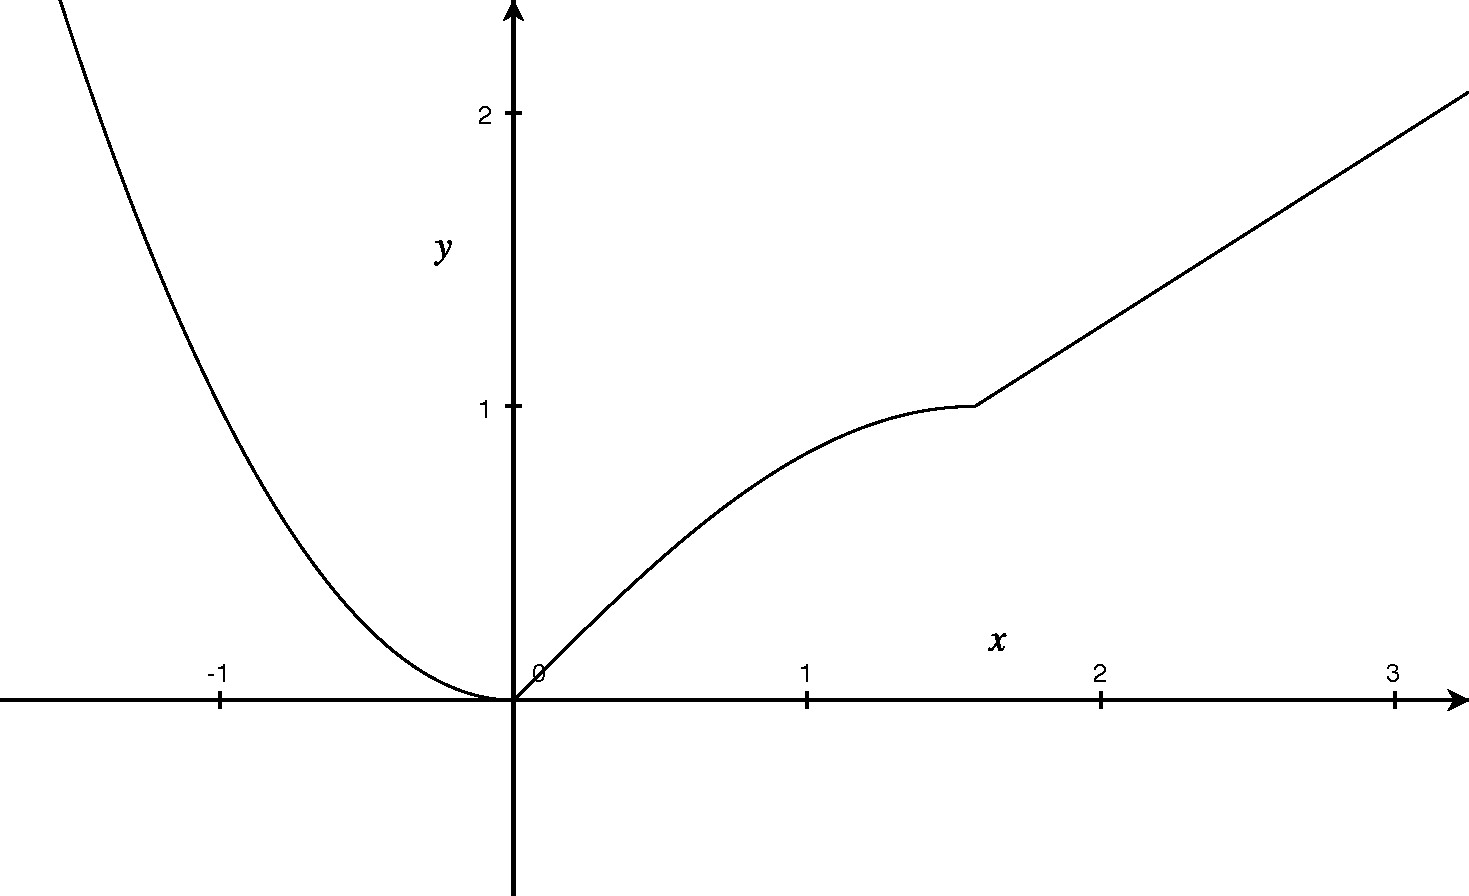
\includegraphics[width=4in]{./graphics/graph0401.pdf} 
   \caption{Partial graph of $f\left( x \right)$.}
   \label{fig:graph0401}
\end{figure}



\subsection{Examples}

\begin{questions}

\question Examine the function
\[
f \left( x \right) = \left\{ {\begin{array}{lcl}
  {x^2} & {\mbox{if}} & x < 1\\
  {1 + \ln x} & {\mbox{if}} & 1 \leq x < e\\
  {x} & {\mbox{if}} & x \geq e
\end{array}} \right.
\]
at the points where $x=1$ and $x=e$.

\begin{solution}
This will be discussed in class.
\end{solution}

\question Are there values of $c$ and $m$ that make
\[
h \left( x \right) = \left\{ {\begin{array}{lcl}
  {cx^2} & {\mbox{if}} & x < 1\\
  {4} & {\mbox{if}} & x=1\\
  {mx-x^3} & {\mbox{if}} & x >1
\end{array}} \right.
\]
continuous at $x=1$? If so. what are the values of $c$ and $m$?

\begin{solution}
This will be discussed in class.
\end{solution}


\question Show that
\[
f \left( x \right) = \frac{x^4 - 1}{x-1}
\]
is discontinuous at $x=1$. Rewrite this function (piecewise defined) so that it is continuous everywhere (remove the point discontinuity).

\begin{solution}
The function is not defined at $x=1$, it has a removable discontinuity because
\[
\lim_{x \to 1} f \left( x \right) = 4.
\]
We need to plug the hole at $x=1$.
\[
h \left( x \right) = \left\{ {\begin{array}{ccl}
 { \displaystyle \frac{x^4 - 1}{x-1}} & {\mbox{if}} & x \neq 1\\[10pt]
  {4} & {\mbox{if}} & x=1
\end{array}} \right.
\]
\end{solution}

\end{questions}






\subsection{Assignment}
You should read \S  2.4 and do the WebAssign assignment mth.121.02.04.
\vfill
\pagebreak
%*-*-*-*-*-*-*-*-*-*-*-*-*-*-*-*-*-*-*-*-*-*-*-*-*-*-*-*-*-*-*-*-*-*-*-*-*-*-*-*-*-*-*-*-*-*-*-*-*-*-*-*-*-*-*-*-*-*-*-*-*-*-*-*-*-*-*-*-*-*-*-*-*-*-*-*-*-*-*-*-*-*-*-*-

\begin{teacher}
\subsection{Assessments}
The following questions are related to the WebAssign assignments and may be used to assess students' ability. Please do not share any of these questions with students.
\begin{questions}		
\question 	%RogaCalcET2 2.4.001	WA-1701711

Consider the following graph.
\begin{figure}[htbp] %  figure placement: here, top, bottom, or page
   \centering
   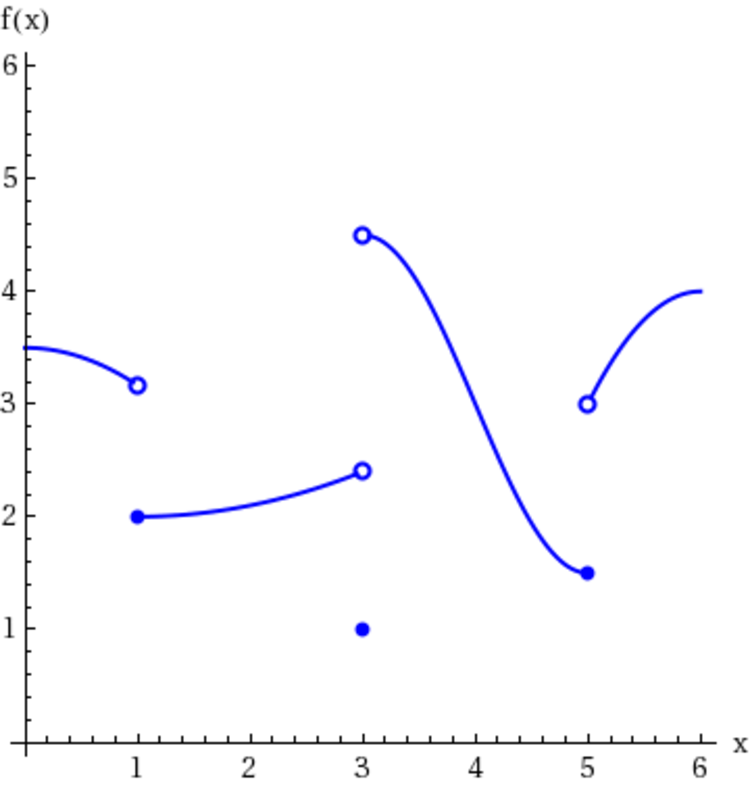
\includegraphics[width=3in]{./graphics/1701711.pdf} 
   \caption{WA-1701711}
   \label{fig:1701711}
\end{figure}

\begin{solution}
\end{solution}

State whether the function shown in the figure is left-continuous only, right-continuous only, continuous, or neither at the following points:
\begin{parts}
\part $x = 1$
\part $x = 3$
\part $x = 5$
\end{parts}

\begin{solution}
\end{solution}

\question 	%RogaCalcET2 2.4.006	WA-1725310

Let $f\left(x\right)$ be the function
\[
f\left( x \right) =
\left\{
{\begin{array}{*{20}{r}}
4 & \text{for} & x < 3\\
- 1 & \text{for} & x > 3
\end{array}}
\right.
\]
Determine the value of $f\left( 3 \right)$ if $f$ is right-continuous at $x = 3$.



\begin{solution}
\end{solution}

\question 	%RogaCalcET2 2.4.009	WA-1701660

Use the Laws of Continuity to determine whether the function is continuous or discontinuous.
\[
f\left(x\right) = 3x + 5 \cos x
\]


\begin{solution}
\end{solution}

\question 	%RogaCalcET2 2.4.011	WA-1701536

Use the Laws of Continuity to determine whether the function is continuous or discontinuous.
\[
f\left(x\right) = -\frac{3}{3x^2+4}
\]


\begin{solution}
\end{solution}

\question 	%RogaCalcET2 2.4.013	WA-1701707

Use the Laws of Continuity to determine whether the function is continuous or discontinuous.
\[
f\left(x\right) = -\frac{3^x}{4^x-3}
\]


\begin{solution}
\end{solution}

\question 	%RogaCalcET2 2.4.017	WA-1710980

Determine the points at which the function is discontinuous.
\[
f\left(x\right) = \frac{1}{x-3}
\] 
Classify these as removable, jump, or infinite discontinuities.


\begin{solution}
\end{solution}

\question 	%RogaCalcET2 2.4.022	WA-1710981

Determine the points at which the function is discontinuous
\[
f\left(t\right) = \frac{2}{t^2 - 3t}
\]
Classify these as removable, jump, or infinite discontinuities.


\begin{solution}
\end{solution}

\question 	%RogaCalcET2 2.4.025	WA-1701685

Is the following statement true or false?
The function $f\left(x\right) = 2x^{3/2} - 7x^3$ is right-continuous at $x = 0$.


\begin{solution}
\end{solution}

\question 	%RogaCalcET2 2.4.027	WA-1725578

Determine the points at which the function $f\left(x\right)$ is discontinuous.
\[
f\left( x \right) =
\left\{
{\begin{array}{ccc}
\displaystyle \frac{x-3}{\left| x - 3 \right|} & \text{for} & x \neq 3\\[10pt]
- 9 & \text{for} & x = 3
\end{array}}
\right.
\]
State the type of discontinuity.


\begin{solution}
\end{solution}

\question 	%RogaCalcET2 2.4.028	WA-1726838

Determine the points at which the function $f\left(x\right)$ is discontinuous.
\[
f\left( x \right) =
\left\{
{\begin{array}{ccc}
\displaystyle \sin \left( \frac{1}{x-4}\right) & \text{for} & x \neq 4\\[10pt]
0 & \text{for} & x = 4
\end{array}}
\right.
\]
State the type of discontinuity.


\begin{solution}
\end{solution}

\question 	%RogaCalcET2 2.4.033	WA-1710975

Determine the points at which the function is discontinuous.
\[
f\left(x\right) = \frac{4}{e^{2x} - e^{-x+3}}
\]
Classify these as removable, jump, or infinite discontinuities.


\begin{solution}
\end{solution}

\question 	%RogaCalcET2 2.4.036	WA-1747166

Determine the domain of the function $f\left(x\right) = \sqrt{3x^2 - 27}$.


\begin{solution}
\end{solution}

\question 	%RogaCalcET2 2.4.038	WA-1739392

Determine the domain of the function $f\left(x\right) = \displaystyle \frac{4x^3}{5x-x^{1/2}}$.


\begin{solution}
\end{solution}

\question 	%RogaCalcET2 2.4.051	WA-1711570

Let $f\left(x\right)$ be the function
\[
f\left( x \right) =
\left\{
{\begin{array}{ccc}
3x^2 & \text{for} & x \leq 2\\[10pt]
4-x & \text{for} & x >2
\end{array}}
\right.
\]
Compute the right- and left-hand limits at $x = 2$.
\begin{parts}
\part $\displaystyle \lim_{x \to 2^+} f\left( x \right)=$

\begin{solution}
\end{solution}

\part $\displaystyle \lim_{x \to 2^-} f\left( x \right)=$

\begin{solution}
\end{solution}

\end{parts}
Determine whether $f\left( x \right)$ is right-continuous, left-continuous, continuous, or neither at that point.


\begin{solution}
\end{solution}

\question 	%RogaCalcET2 2.4.057	WA-1725318

Let $f\left(x\right)$ be the function
\[
f\left( x \right) =
\left\{
{\begin{array}{ccc}
x^2 - c & \text{for} & x < 4 \\[10pt]
6x + 4c & \text{for} & x  \geq 4
\end{array}}
\right.
\]
Find the value of $c$ that makes the function continuous.

\begin{solution}
\end{solution}


\question 	%RogaCalcET2 2.4.080	WA-1711463

Evaluate the limit using the substitution method.
\[
\lim_{x \to 0} 6 \arctan e^x
\]

\begin{solution}
\end{solution}

\question 	%RogaCalcET2 2.4.084	WA-1711460

See problem 84 in \S2.4.

\begin{solution}
\end{solution}

\end{questions}
\end{teacher}

\vfill
\pagebreak

%*-*-*-*-*-*-*-*-*-*-*-*-*-*-*-*-*-*-*-*-*-*-*-*-*-*-*-*-*-*-*-*-*-*-*-*-*-*-*-*-*-*-*-*-*-*-*-*-*-*-*-*-*-*-*-*-*-*-*-*-*-*-*-*-*-*-*-*-*-*-*-*-*-*-*-*-*-*-*-*-*-*-*-*-
\section{mth.121.02.05}
\subsection{Algebraic Manipulation and Reason!}


\textbf{Example:} Supposed you're asked to find the following limit.
\[
\lim_{x \to 1} \left( \frac{1}{x-1} - \frac{2}{x^2-1} \right)
\]
And you just plug the number in and you're then faced with $\infty - \infty$. You may believe you're looking at $0$, but its's actually $1/2$. So it looks like these infinities battle one another and when the dust settled you were left with $1/2$, not $0$ as some (mindless people) may conclude. Here, like many limit problems, you'll need to use your algebra skills to reason forward.



\begin{solution}

\begin{eqnarray*}
\lim_{x \to 1} \left( \frac{1}{x-1} - \frac{2}{x^2-1} \right) &=& \lim_{x \to 1} \frac{\left( x -1 \right)}{\left( x -1 \right)\left( x +1 \right)}\\
&=&  \lim_{x \to 1} \frac{1}{ x +1} = \frac{1}{2}
\end{eqnarray*}
\end{solution}

In the examples that follow, we will be faced with problems where thinking is \emph{required}. I strongly suggest that you think before answering. And when you're faced with $0/0$, $\infty/\infty$, $\infty \cdot 0$, and $\infty - \infty$ \dots \emph{you're really going to have to think.}\footnote{Indeterminate forms.} Yes, your numerical and algebraic skills will be needed.

\subsection{Examples}

\begin{questions}
\question Find the limit if it exist.
\[
\mathop {\lim }\limits_{x \to 0^+}  \frac{\left| x \right|}{x}
\]

\begin{solution}
We'll discuss this in class

Final Answer.
\[
\mathop {\lim }\limits_{x \to 0^+}  \frac{\left| x \right|}{x} =1
\]
\end{solution}


\question Find the limit if it exist.
\[
\mathop {\lim }\limits_{x \to 0^-}  \frac{\left| x \right|}{x}
\]

\begin{solution}
We'll discuss this in class

Final Answer.
\[
\mathop {\lim }\limits_{x \to 0^-}  \frac{\left| x \right|}{x} = -1
\]
\end{solution}

\question Find the limit if it exist.
\[
\mathop {\lim }\limits_{x \to 0}  \frac{\left| x \right|}{x}
\]

\begin{solution}
We'll discuss this in class

Final Answer.
\[
\mathop {\lim }\limits_{x \to 0}  \frac{\left| x \right|}{x} = DNE
\]
\end{solution}


\question Find the limit if it exist.
\[
\lim_{x \to 8} \frac{x^3-64x}{x-8}
\]

\begin{solution}
We'll discuss this in class

Final Answer.
\[
\lim_{x \to 8} \frac{x^3-64x}{x-8} = 128
\]
\end{solution}

\question Find the limit if it exist.
\[
\lim_{x \to 0} \frac{\left(1+x\right)^3-1}{x}
\]

\begin{solution}
We'll discuss this in class

Final Answer.
\[
\lim_{x \to 0} \frac{\left(1+x\right)^3-1}{x} = 3
\]
\end{solution}


\question Find the limit if it exist.
\[
\lim_{x \to 1} \frac{3^{2x}-9}{3^x-3}
\]

\begin{solution}
We'll discuss this in class

Final Answer.
\[
\lim_{x \to 1} \frac{3^{2x}-9}{3^x-3} = 6
\]
\end{solution}


\question Find the limit if it exist.
\[
\lim_{x \to 0^+} \left(\frac{1}{\sqrt{x}} - \frac{1}{\sqrt{x^2+x}}\right)
\]

\begin{solution}
We'll discuss this in class

Final Answer.
\[
\lim_{x \to 0^+} \left(\frac{1}{\sqrt{x}} - \frac{1}{\sqrt{x^2+x}}\right) =0
\]
\end{solution}


\question Find the limit if it exist.
\[
\lim_{x \to \pi/2} \frac{\cot x}{\csc x}
\]

\begin{solution}
We'll discuss this in class

Final Answer.
\[
\lim_{x \to \pi/2} \frac{\cot x}{\csc x} =0
\]
\end{solution}








\question Given
\[
f \left( x \right) = \left\{ {\begin{array}{ccc}
   {2x} & {\mbox{if}} & {x<2}  \\
   {x^2} & {\mbox{if}} & {x \geq2 }  ,
 \end{array} } \right.
\]
find each of the following if it exist.
\begin{parts}
\part
\[
\mathop {\lim }\limits_{x \to 2^-}  f \left( x \right)
\]

\begin{solution}
We'll discuss this in class

Final Answer.
\[
\mathop {\lim }\limits_{x \to 2^-}  f \left( x \right) = 4
\]
\end{solution}

\part
\[
\mathop {\lim }\limits_{x \to 2^+}  f \left( x \right)
\]

\begin{solution}
We'll discuss this in class

Final Answer.
\[
\mathop {\lim }\limits_{x \to 2^+}  f \left( x \right)=4
\]
\end{solution}

\part
\[
\mathop {\lim }\limits_{x \to 2}  f \left( x \right)
\]

\begin{solution}
We'll discuss this in class

Final Answer.
\[
\mathop {\lim }\limits_{x \to 2}  f \left( x \right)=4
\]
\end{solution}

\part
\[
f \left( 2 \right)
\]

\begin{solution}
We'll discuss this in class

Final Answer.
\[
f \left( 2 \right)=4
\]
\end{solution}

\end{parts}

\question Find the limit if it exist.
\[
\mathop {\lim }\limits_{x \to -1}  \frac{x^2-1}{x+1}
\]

\begin{solution}
We'll discuss this in class

Final Answer.
\[
\mathop {\lim }\limits_{x \to -1}  \frac{x^2-1}{x+1} = -2
\]
\end{solution}

\question Find the limit if it exist.
\[
\mathop {\lim }\limits_{x \to 0}  \frac{x^2+4x}{\sqrt{x^3+x^2}}
\]

\begin{solution}

Final Answer.
\[
\lim_{x \to 0}  \frac{x^2+4x}{\sqrt{x^3+x^2}}=DNE
\]
The following work would be expected if this were an exam question.
\begin{enumerate}
\item For $x > 0$ (from the right of $0$) we have
\[
\lim_{x \to 0^+}  \frac{x^2+4x}{\sqrt{x^3+x^2}}= \lim_{x \to 0^+}  \frac{x \left( x + 4 \right)}{x\sqrt{x+1}} = \lim_{x \to 0^+}  \frac{x + 4}{\sqrt{x+1}} = 4
\]
\item For $x < 0$ (from the left of $0$) we have
\[
\lim_{x \to 0^-}  \frac{x^2+4x}{\sqrt{x^3+x^2}}= \lim_{x \to 0^-}  \frac{x \left( x + 4 \right)}{-x\sqrt{x+1}} = \lim_{x \to 0^-}  \frac{-x - 4}{\sqrt{x+1}} = -4
\]
\end{enumerate}
Knowing that $\sqrt{x^2} = \left| x \right|$ is certainly helpful, but so is a graph (Figure \ref{fig:new005}, page \pageref{fig:new005}) of
\[
f\left( x \right) = \frac{x^2+4x}{\sqrt{x^3+x^2}}.
\]
\end{solution}
\begin{figure}[htbp] %  figure placement: here, top, bottom, or page
   \centering
   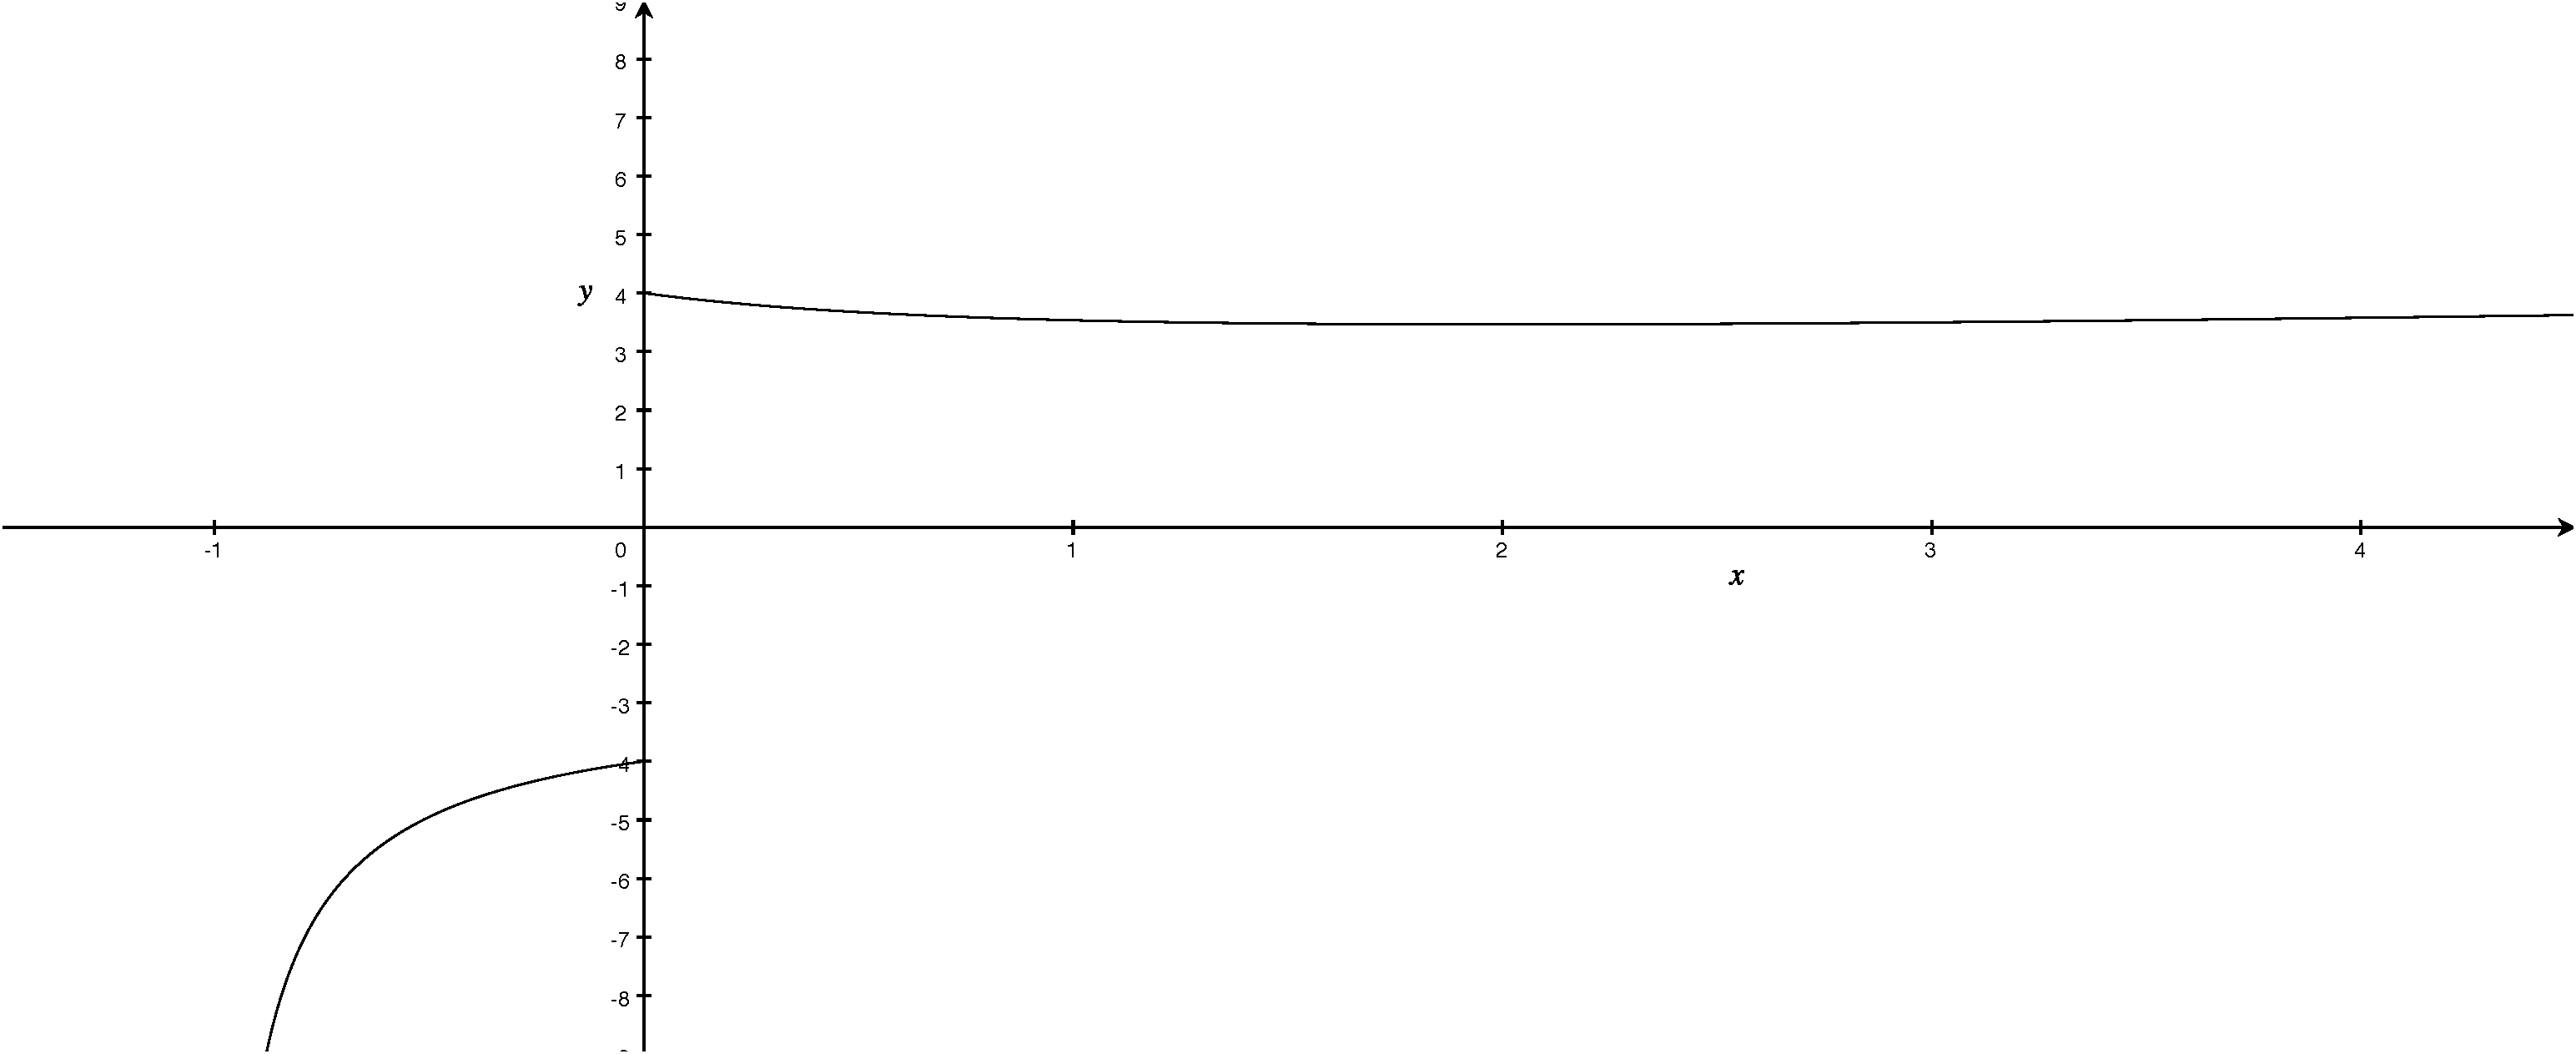
\includegraphics[width=4in]{./graphics/new005.pdf} 
   \caption{Convincing graph?}
   \label{fig:new005}
\end{figure}



\question Find the limit if it exist.
\[
\mathop {\lim }\limits_{x \to 0}  \frac{x e^{1-2x}}{x^2+x}
\]

\begin{solution}
We'll discuss this in class

Final Answer.
\[
\mathop {\lim }\limits_{x \to 0}  \frac{x e^{1-2x}}{x^2+x} = e
\]
\end{solution}

\question Find the limit if it exist.
\[
\mathop {\lim }\limits_{x \to 0}  \left( \frac{2}{x} - \frac{2}{\left| x \right|} \right)
\]

\begin{solution}
We'll discuss this in class

Final Answer.
\[
\mathop {\lim }\limits_{x \to 0}  \left( \frac{2}{x} - \frac{2}{\left| x \right|} \right)=DNE
\]
Again, on exams you will need to show two limits to reach this conclusion.
\begin{enumerate}
\item For $x > 0$ (from the right of $0$) we have
\[
\mathop {\lim }\limits_{x \to 0^+}  \left( \frac{2}{x} - \frac{2}{\left| x \right|} \right) = \mathop {\lim }\limits_{x \to 0^+}  \left( \frac{2}{x} - \frac{2}{ x } \right) = 0 
\]
\item For $x < 0$ (from the left of $0$) we have
\[
\mathop {\lim }\limits_{x \to 0^-}  \left( \frac{2}{x} - \frac{2}{\left| x \right|} \right) = \mathop {\lim }\limits_{x \to 0^-}  \left( \frac{2}{x} + \frac{2}{ x } \right) =  \mathop {\lim }\limits_{x \to 0-}   \frac{4}{x} = - \infty
\]
\end{enumerate}
\end{solution}

\question Find the limit if it exist.
\[
\mathop {\lim }\limits_{x \to 4^+}  \sqrt{16-x^2}
\]

\begin{solution}
We'll discuss this in class

Final Answer.
\[
\mathop {\lim }\limits_{x \to 4^+}  \sqrt{16-x^2} = DNE
\]
\end{solution}

\question Find the limit if it exist.
\[
\mathop {\lim }\limits_{x \to 4^-}  \sqrt{16-x^2}
\]

\begin{solution}
We'll discuss this in class

Final Answer.
\[
\mathop {\lim }\limits_{x \to 4^-}  \sqrt{16-x^2} = 0
\]
\end{solution}

\question Given that $\displaystyle  \mathop {\lim }\limits_{x \to 0}  \frac{\sin x}{x} = 1$,
find
\[
\mathop {\lim }\limits_{x \to 0}  \frac{1 - \cos^2 x}{x^2}.
\]

\begin{solution}
We'll discuss this in class


\begin{eqnarray*}
\lim_{x \to 0}  \frac{1 - \cos^2 x}{x^2} &=& \lim_{x \to 0}  \frac{\sin^2 x}{x^2}\\
&=& \lim_{x \to 0}  \frac{\sin x}{x} \cdot \frac{\sin x}{x} =1
\end{eqnarray*}

\end{solution}

\end{questions}













\subsection{Assignment}
You should read \S  2.5 and do the WebAssign assignment mth.121.02.05.
\vfill
\pagebreak
%*-*-*-*-*-*-*-*-*-*-*-*-*-*-*-*-*-*-*-*-*-*-*-*-*-*-*-*-*-*-*-*-*-*-*-*-*-*-*-*-*-*-*-*-*-*-*-*-*-*-*-*-*-*-*-*-*-*-*-*-*-*-*-*-*-*-*-*-*-*-*-*-*-*-*-*-*-*-*-*-*-*-*-*-

\begin{teacher}
\subsection{Assessments}
The following questions are related to the WebAssign assignments and may be used to assess students' ability. Please do not share any of these questions with students.
\begin{questions}	
\question 	%RogaCalcET2 2.5.001	WA-1715890

Evaluate the limit or state that it does not exist. (If an answer does not exist, enter DNE.)
\[
\lim_{x \to 6} \frac{x^2 - 36}{x - 6}
\]


\begin{solution}
\end{solution}

\question 	%RogaCalcET2 2.5.003	WA-1715911

Evaluate the limit or state that it does not exist.
\[
\lim_{x \to -8} \frac{x^2+17x+72}{x +8 }
\]



\begin{solution}
\end{solution}

\question 	%RogaCalcET2 2.5.006	WA-1701618

Evaluate the limit or state that it does not exist.
\[
\lim_{x \to 5} \frac{x^2-25}{x -7 }
\]


\begin{solution}
\end{solution}

\question 	%RogaCalcET2 2.5.009	WA-1715934

Evaluate the limit or state that it does not exist.
\[
\lim_{x \to 3} \frac{2x^2+8x-42}{x^2-9 }
\]


\begin{solution}
\end{solution}

\question 	%RogaCalcET2 2.5.010	WA-1715931

Evaluate the limit or state that it does not exist.
\[
\lim_{x \to 0} \frac{\left(2+3x\right)^3-8}{x }
\]


\begin{solution}
\end{solution}

\question 	%RogaCalcET2 2.5.012	WA-1715915

Evaluate the limit or state that it does not exist.
\[
\lim_{x \to 5} \frac{x^2-x}{x^2-25 }
\]


\begin{solution}
\end{solution}

\question 	%RogaCalcET2 2.5.015	WA-1718592

Evaluate the limit or state that it does not exist.
\[
\lim_{x \to 0} \frac{6^{2x}-1}{6^x-1}
\]


\begin{solution}
\end{solution}

\question 	%RogaCalcET2 2.5.018	WA-1701658

Evaluate the limit or state that it does not exist.
\[
\lim_{h \to 0} \frac{\left(h+3\right)^{-2} - 9^{-1}}{h}
\]


\begin{solution}
\end{solution}

\question 	%RogaCalcET2 2.5.021	WA-1701517

Evaluate the limit or state that it does not exist.
\[
\lim_{x \to 7} \frac{x-7}{\sqrt{x} -\sqrt{14-x} }
\]


\begin{solution}
\end{solution}

\question 	%RogaCalcET2 2.5.024	WA-1689418

Evaluate the limit or state that it does not exist.
\[
\lim_{x \to 49} \frac{\sqrt{50-x} - 1}{7-\sqrt{x} }
\]


\begin{solution}
\end{solution}

\question 	%RogaCalcET2 2.5.025	WA-1702657

Evaluate the limit or state that it does not exist.
\[
\lim_{x \to 16} \left( \frac{1}{\sqrt{x}-4} - \frac{8}{x-16} \right)
\]


\begin{solution}
\end{solution}

\question 	%RogaCalcET2 2.5.027	WA-1701680

Evaluate the limit or state that it does not exist.
\[
\lim_{x \to 0} \frac{\cot 5x}{\csc 5x}
\]


\begin{solution}
\end{solution}

\question 	%RogaCalcET2 2.5.028	WA-1701749

Evaluate the limit or state that it does not exist.
\[
\lim_{\theta \to \pi/2} \frac{\cot 7 \theta}{\csc 7 \theta}
\]


\begin{solution}
\end{solution}

\question 	%RogaCalcET2 2.5.030	WA-1715965

Evaluate the limit or state that it does not exist.
\[
\lim_{x \to 1} \left( \frac{18}{1-x} - \frac{36}{1-x^2} \right)
\]


\begin{solution}
\end{solution}

\question 	%RogaCalcET2 2.5.045	WA-1701602

Evaluate the limit or state that it does not exist.
\[
\lim_{t \to -1} \left( 3t - 2at + 4a \right)
\]


\begin{solution}
\end{solution}

\question 	%RogaCalcET2 2.5.049	WA-1701628

Evaluate the limit or state that it does not exist.
\[
\lim_{x \to 0} \frac{3\left(x+h\right)^2-3x^2}{h}
\]


\begin{solution}
\end{solution}

\question 	%RogaCalcET2 2.5.054	WA-1701574

Evaluate the limit or state that it does not exist.
\[
\lim_{x \to a} \frac{2x^{-1}-2a^{-1}}{x-a}
\]


\begin{solution}
\end{solution}

\end{questions}

\end{teacher}
\vfill
\pagebreak

%*-*-*-*-*-*-*-*-*-*-*-*-*-*-*-*-*-*-*-*-*-*-*-*-*-*-*-*-*-*-*-*-*-*-*-*-*-*-*-*-*-*-*-*-*-*-*-*-*-*-*-*-*-*-*-*-*-*-*-*-*-*-*-*-*-*-*-*-*-*-*-*-*-*-*-*-*-*-*-*-*-*-*-*-
\section{mth.121.02.06}
\subsection{Trigonometric Limits}

\subsubsection{Squeeze Theorem}
On occasion we will be asked to evaluate a limit where our \emph{thinking} will fail us, as will the laws. For example, let's say you're asked to evaluate
\[
\mathop {\lim }\limits_{x \to 0^+}
\sqrt{x}\left[ 1 + \sin^2 \left( \frac{2 \pi}{x} \right) \right].
\]
Although this may not seem like a fair question at this \emph{point}, I want to use this example to illustrate a useful technique for evaluating limits. A graph (Figure \ref{fig:graph0602}, page \pageref{fig:graph0602}) of
\[
f\left(x\right) = 
\sqrt{x}\left[ 1 + \sin^2 \left( \frac{2 \pi}{x} \right) \right],
\]
near $x=0$ follows---you should note that $f\left(0\right)$ is undefined, that is, there's a hole at zero.
\begin{figure}[htbp] %  figure placement: here, top, bottom, or page
   \centering
   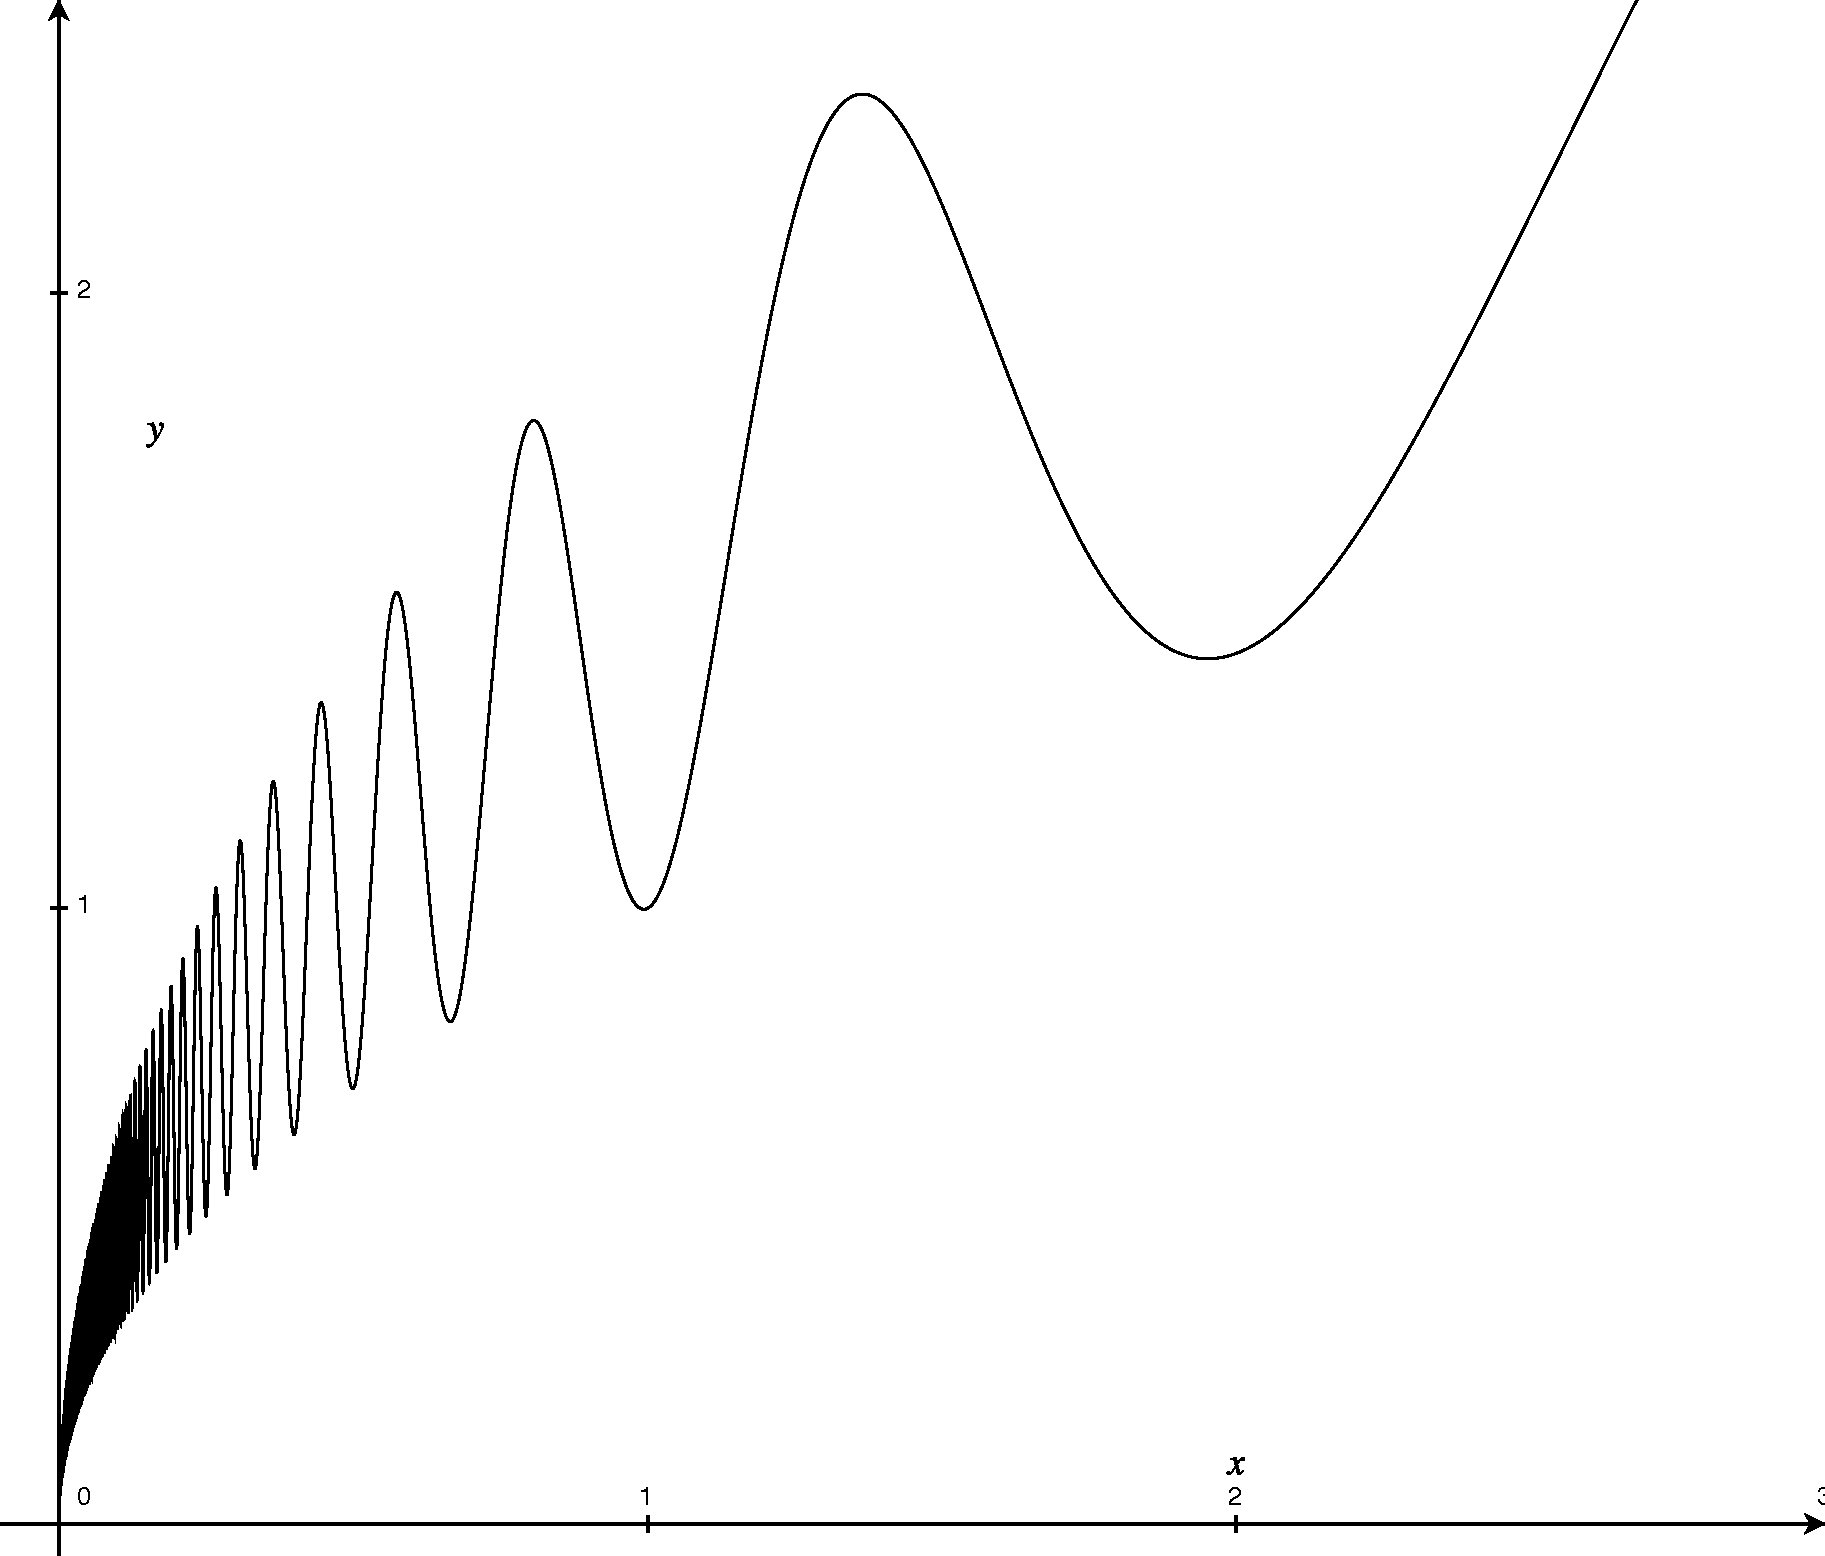
\includegraphics[width=2in]{./graphics/graph0602.pdf} 
   \caption{Partial graph of $f\left(x\right)$.}
   \label{fig:graph0602}
\end{figure}
Try to visualize the hole at $x=0$---you actually can't see the hole, but please don't try to enter this abyss! This abyss is the dreaded division by zero. Yikes!


The main problem here---although easy to guess the limit from this graph---is actually proving that this limit exists and is $0$. To prove this, we need the following theorem.



\textbf{The Squeeze Theorem} states, that if $f \left( x \right) \leq g \left( x \right) \leq h \left( x \right)$ when $x$ is near $a$ (except possibly at $a$) and
\[
\mathop {\lim }\limits_{x \to a} f \left( x \right) = \mathop {\lim }\limits_{x \to a} h \left( x \right) = L
\]
then
\[
\mathop {\lim }\limits_{x \to a} g \left( x \right) = L.
\]



\textbf{Example:} Now let's prove that
\[
\mathop {\lim }\limits_{x \to 0^+}
\sqrt{x}\left[ 1 + \sin^2 \left( \frac{2 \pi}{x} \right) \right] = 0
\]
as our graph clearly indicates.



\begin{solution}
This will be discussed in class! Please try to follow what's being said.
\[
-1 \leq \sin \left( \frac{2 \pi}{x} \right) \leq 1 \quad
\Rightarrow \quad 0 \leq \sin^2 \left( \frac{2 \pi}{x} \right) \leq 1
\quad \Rightarrow \quad 1 \leq 1 + \sin^2 \left( \frac{2 \pi}{x} \right) \leq 2
\]
Now multiply all sides of the last inequality by $\sqrt{x}$, given that $x > 0$ (Since $x$ is from the right of zero, we know that $x > 0$.).
\[
\sqrt{x} \leq \sqrt{x}\left[ 1 + \sin^2 \left( \frac{2 \pi}{x} \right) \right] \leq 2 \sqrt{x}
\]
Since (The limit laws say-so. But, once again, please use your head.)
\[
\mathop {\lim }\limits_{x \to 0^+} \sqrt{x} =
\mathop {\lim }\limits_{x \to 0^+} 2 \sqrt{x} = 0,
\]
we have
\[
\mathop {\lim }\limits_{x \to 0^+}
\sqrt{x}\left[ 1 + \sin^2 \left( \frac{2 \pi}{x} \right) \right] =0
\]
by the Squeeze Theorem.
\end{solution}

\textbf{Illustration:} The red curve (Figure \ref{fig:graph0602}, page \pageref{fig:graph0602}) is $2 \sqrt{x}$; the blue curve is $\sqrt{x}$; and the \emph{squeezed} gray curve in the middle is
\[
\sqrt{x}\left[ 1 + \sin^2 \left( \frac{2 \pi}{x} \right) \right].
\]
I think a graphing utility, whether a calculator or computer, is very helpful.
\begin{figure}[htbp] %  figure placement: here, top, bottom, or page
   \centering
   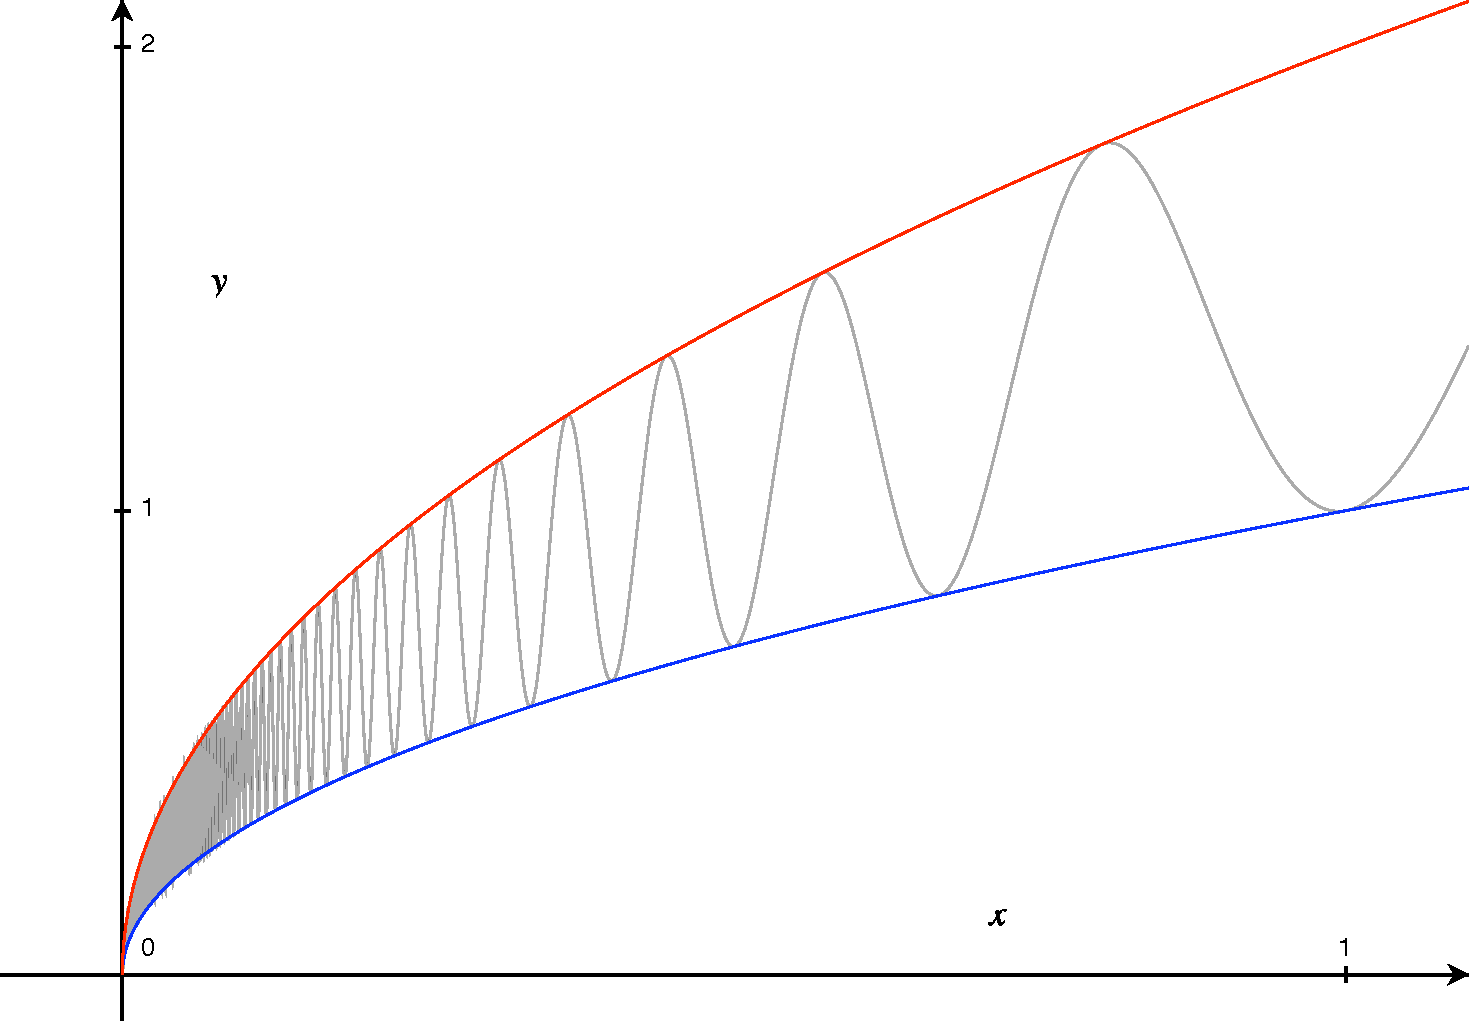
\includegraphics[width=2in]{./graphics/graph0601.pdf} 
   \caption{The Squeeze Theorem visualized!}
   \label{fig:graph0601}
\end{figure}



\subsubsection{An Important Case!}
\[
\mathop {\lim }\limits_{ \theta \to 0} \frac{\sin \theta }{\theta}
\]
If you can recall, you were asked\footnote{You've seen this limit before!} to do this problem numerically and found that it equaled one. Now we need to show this. Here's one way to do so. This is a geometric argument and I am using a \emph{unit} circle and simple area formulas as a basis for this argument.
\begin{figure}[htbp] %  figure placement: here, top, bottom, or page
   \centering
   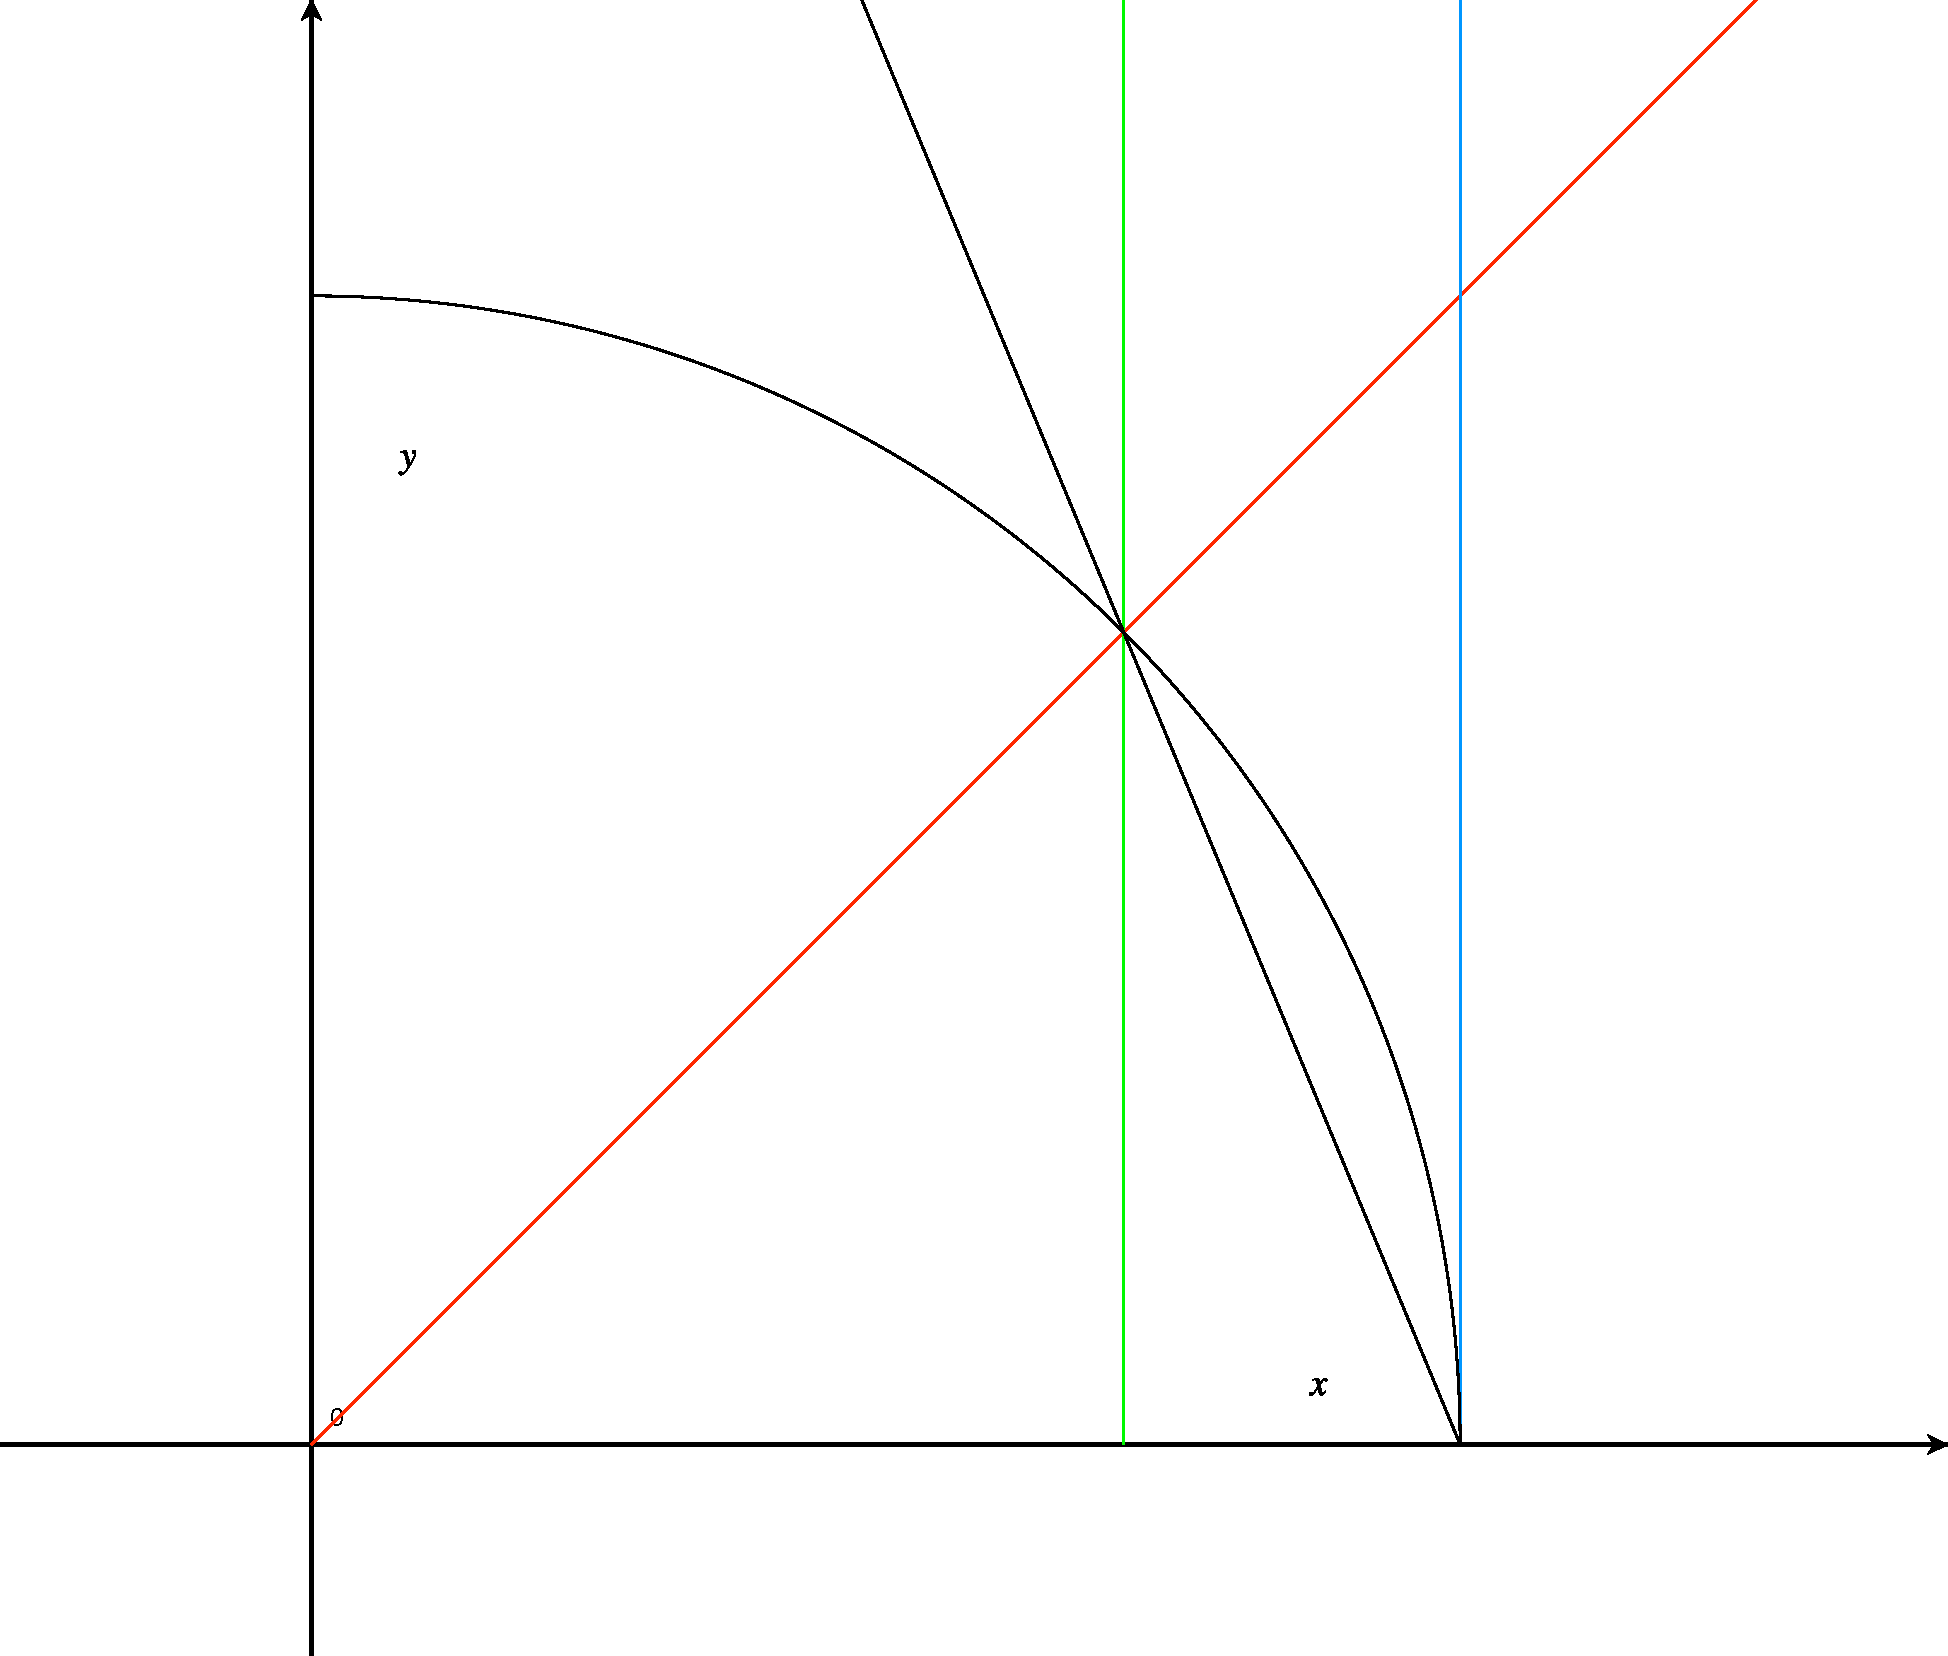
\includegraphics[width=4in]{./graphics/graph0603.pdf} 
   \caption{Will be discussed and labeled in class.}
   \label{fig:graph0603}
\end{figure}
We will label this diagram\footnote{The radius is $1$, that angle is $\theta$, and the point will be labeled using $\sin \theta$ and $\cos \theta$.} in class where I discuss two triangles and one sector.\footnote{You've got to listen to get this!} The inner triangle's area (smallest area triangle---green height, base of $1$) is
\[
\frac{\sin \theta}{2};
\]
the larger sector,\footnote{I hope you can remember your simple trigonometry!}
\[
\frac{\theta}{2};
\]
and finally, a larger area (right triangle---base is $1$ and the height is blue) is
\[
\frac{\tan \theta}{2} = \frac{\sin \theta}{2 \cos \theta}.
\]
When  $0 < \theta < \pi/2$ we get a very simple geometric (areas) inequality
\[
\frac{\sin \theta}{2} < \frac{\theta}{2} < \frac{\sin \theta}{2 \cos \theta},
\]
that can be easily manipulated to:
\[
\cos \theta < \frac{\sin \theta}{\theta} < 1.
\]
This inequality also holds for $-\pi/2 < \theta < 0$.\footnote{A good argument here can either be geometric, or noting  the even nature of our relationship.}
Now just use the Squeeze Theorem to finally show that
\[
\mathop {\lim }\limits_{ \theta \to 0} \frac{\sin \theta }{\theta} = 1.
\]
You'll need to remember this!



That was a lot of work and this limit will pop up often in calculus, so remember it!

\textbf{Example:} In fact this limit can be used to show that
\[
\mathop {\lim }\limits_{ \theta \to 0} \frac{ \cos \theta - 1}{\theta} = 0.
\]



\begin{solution}
\begin{eqnarray*}
\lim_{ \theta \to 0} \frac{ \cos \theta - 1}{\theta} &=& \lim_{ \theta \to 0} \frac{ \cos \theta - 1}{\theta} \cdot \frac{\cos \theta + 1}{\cos \theta + 1} \\
&=& \lim_{ \theta \to 0} - \frac{\sin^2 \theta}{\theta \left( \cos \theta + 1 \right)}\\
&=& \lim_{ \theta \to 0} - \frac{\sin \theta}{\theta} \cdot \frac{\sin \theta}{ \left( \cos \theta + 1 \right)} = 0
\end{eqnarray*}

\end{solution}


\subsection{Examples}

\begin{questions}

\question Evaluate.
\[
\mathop {\lim }\limits_{x \to 0}  \frac{\csc 8x}{ \csc 4x}
\]

\begin{solution}
We'll discuss this in class.

\begin{eqnarray*}
 \lim_{x \to 0}  \frac{\csc 8x}{ \csc 4x} &=&  \lim_{x \to 0}  \frac{\sin 4x}{ \sin 8x}\\
&=&  \lim_{x \to 0}  \frac{\sin 4x}{ 4x} \cdot \frac{8x}{ \sin 8x} \cdot \frac{4x}{8x} \\
&=& \frac{1}{2}
\end{eqnarray*}

\end{solution}


\question Evaluate using the Squeeze Theorem.
\[
\lim_{x \to 3} \left(x^2-9\right) \frac{x-3}{\left| x-3\right|}
\]

\begin{figure}[htbp] %  figure placement: here, top, bottom, or page
   \centering
   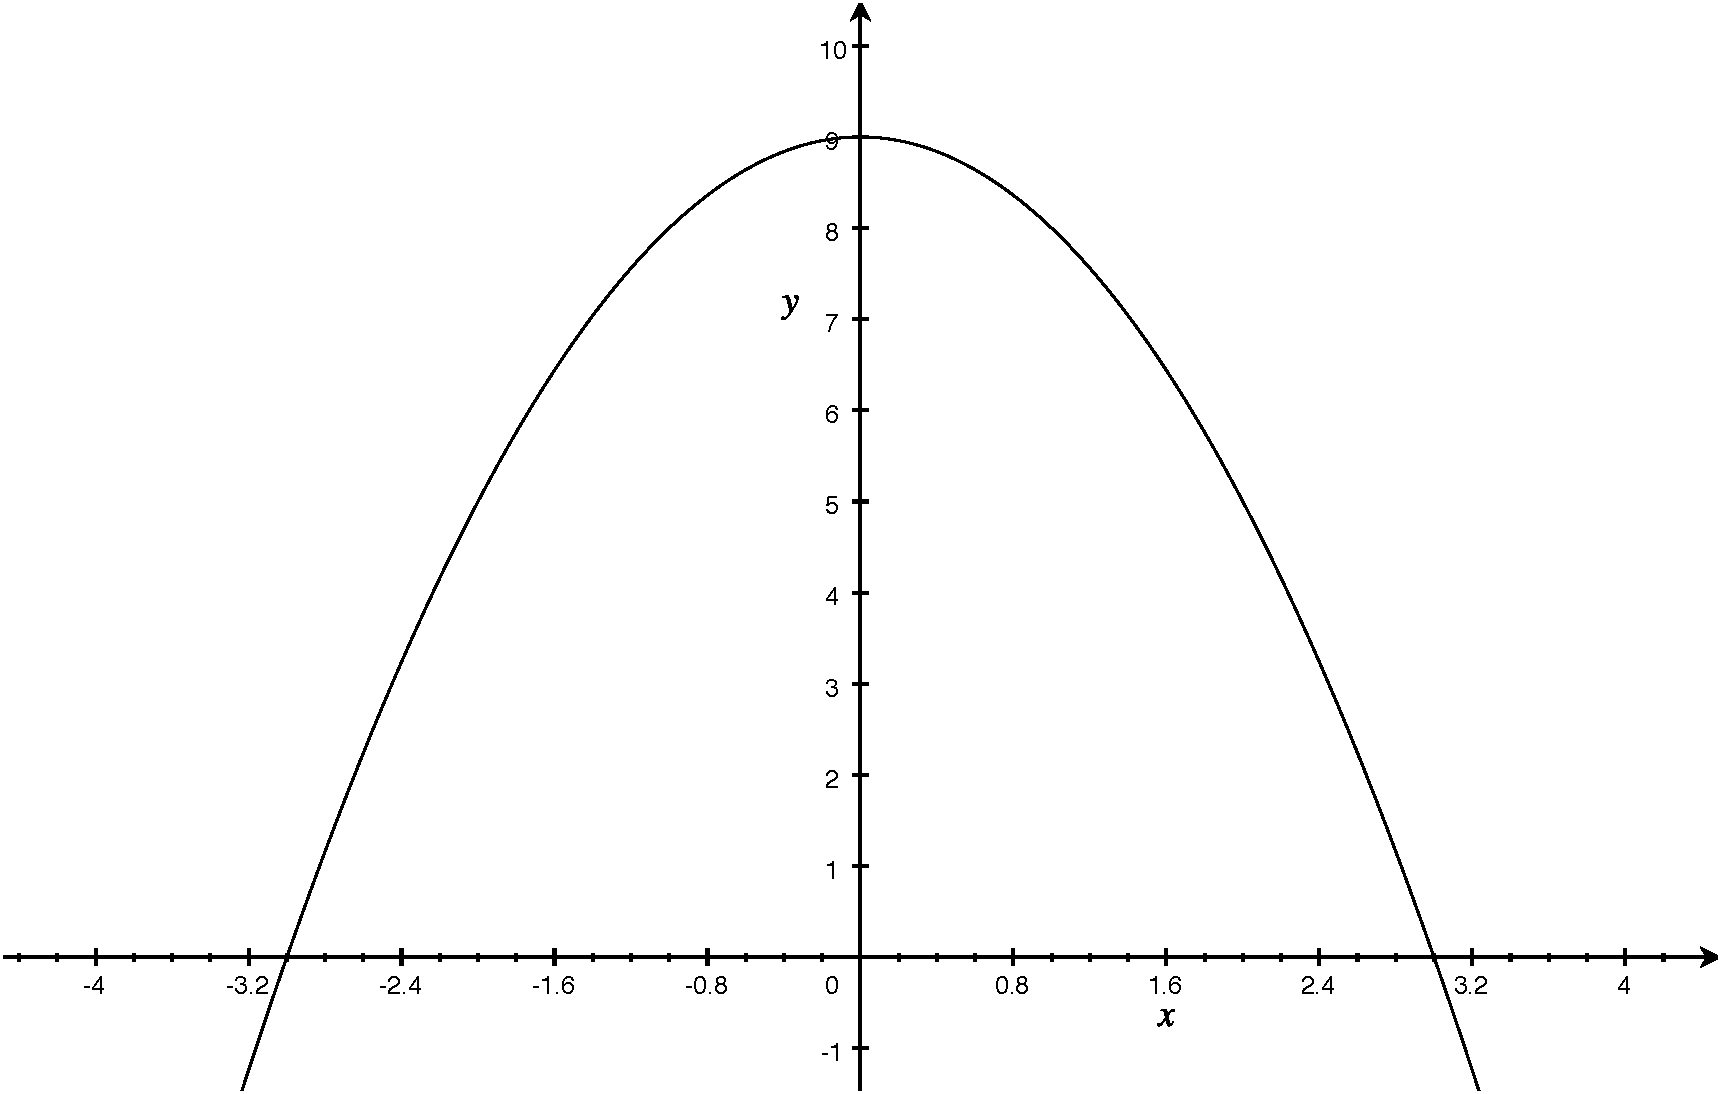
\includegraphics[width=2in]{./graphics/graphst01.pdf}
   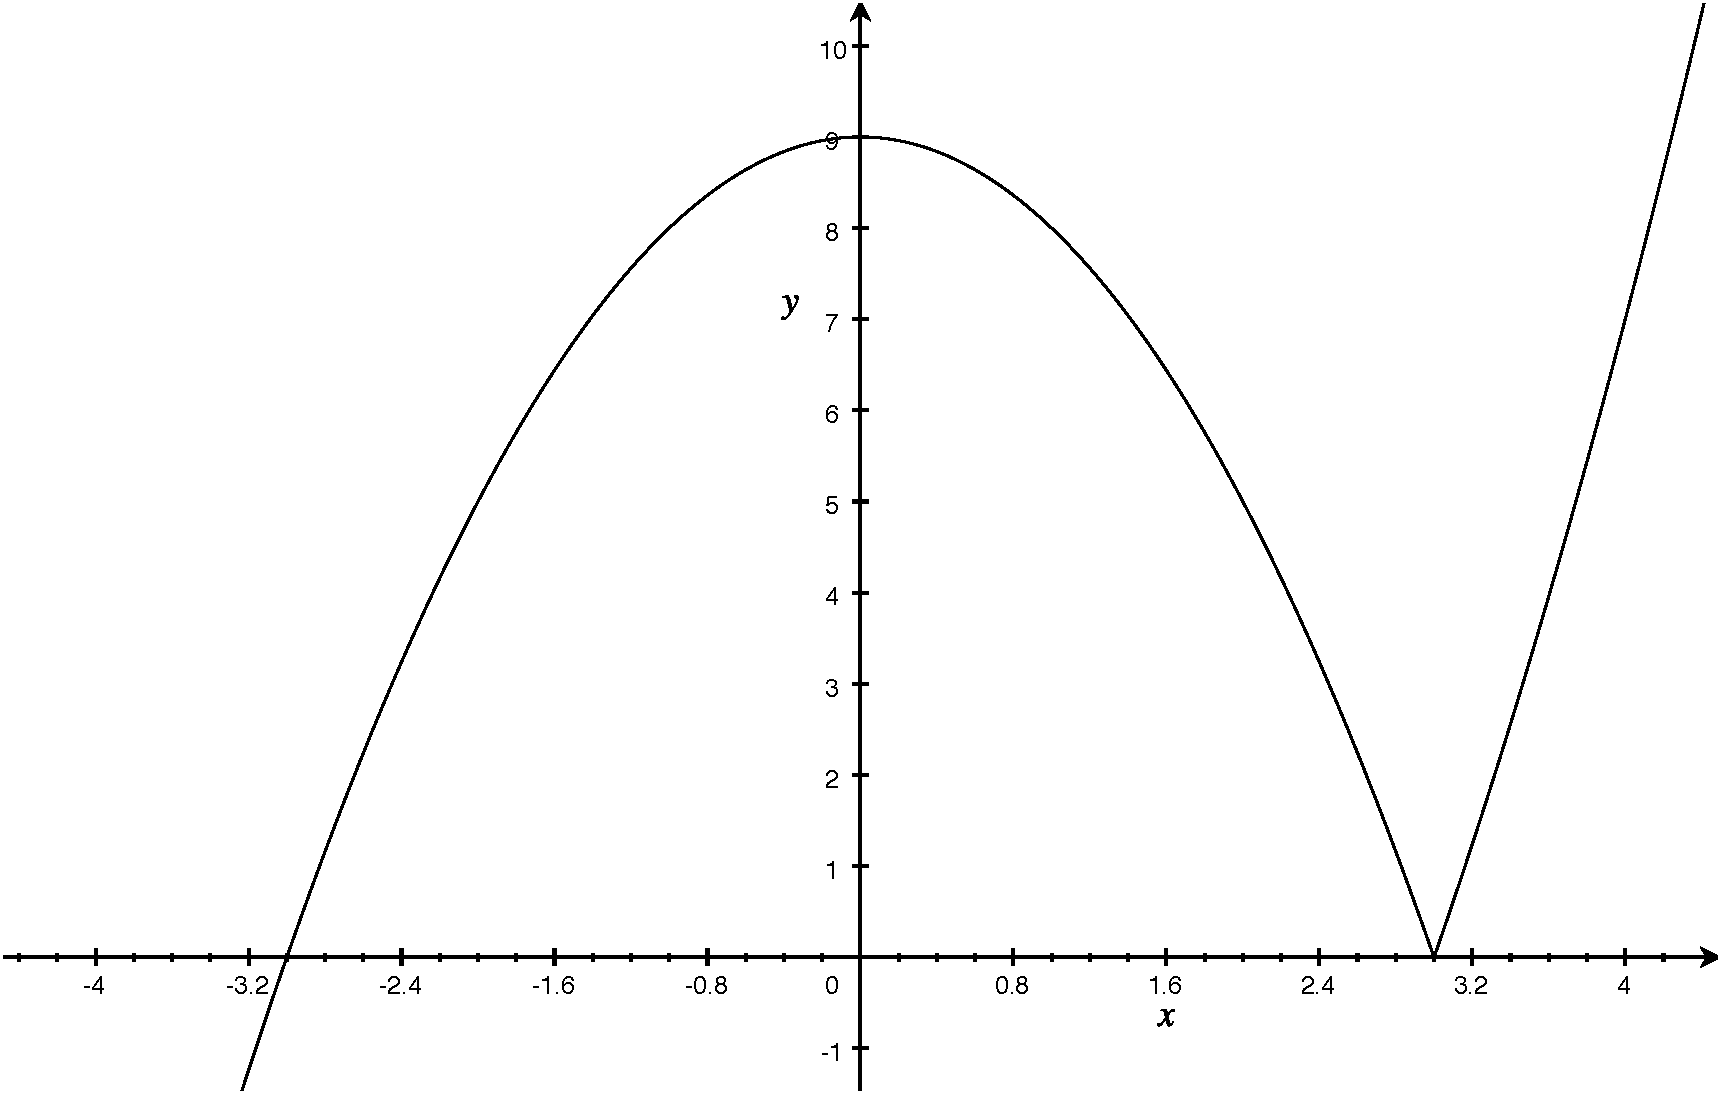
\includegraphics[width=2in]{./graphics/graphst03.pdf}
   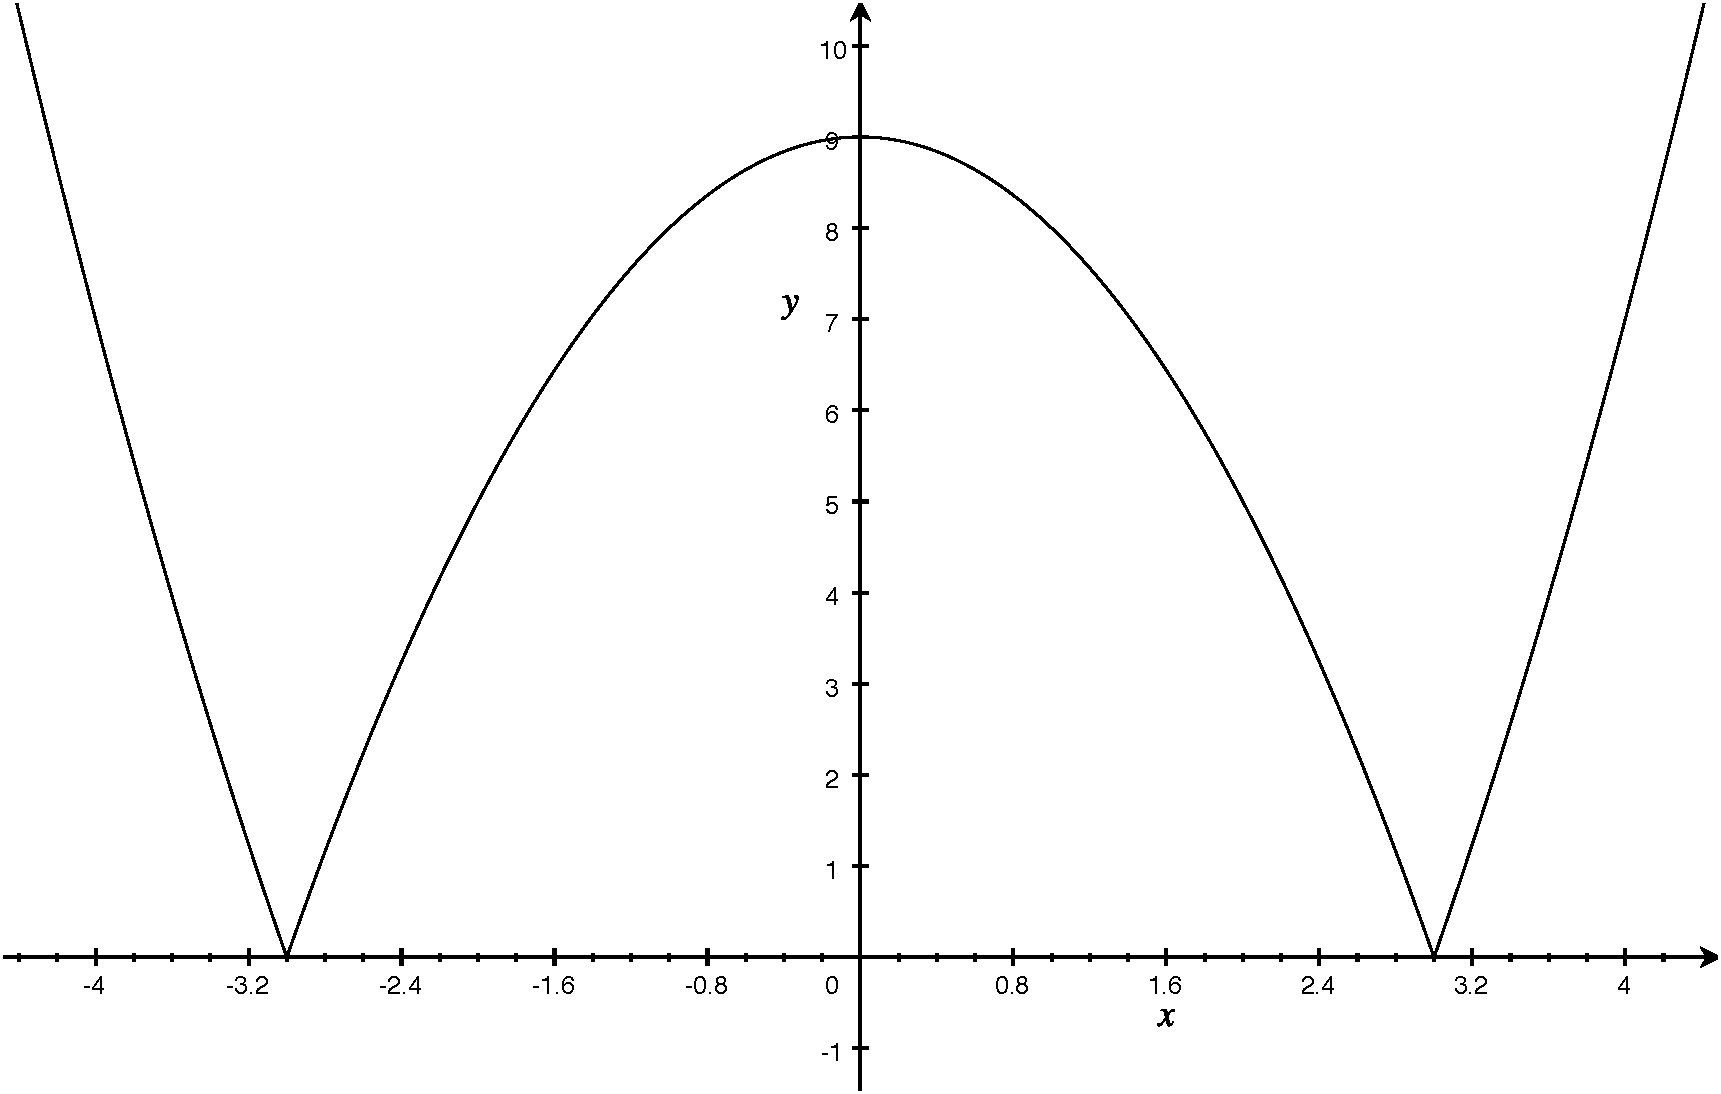
\includegraphics[width=2in]{./graphics/graphst02.pdf}
   \caption{$y_1 =9-x^2$,  $y_2 = \left(x^2-9\right) \displaystyle \frac{x-3}{\left| x-3\right|}$ and $y_3=\left| x^2-9\right|$. Note that $y_1 \leq y_2 \leq y_3$.}
   \label{fig:graphst}
\end{figure}
\begin{solution}
We'll discuss this in class.

It's okay to use a calculator to make sure you're getting a squeeze. It's easy to get tricked!
\begin{eqnarray*}
9-x^2 \leq \left(x^2-9\right) \frac{x-3}{\left| x-3\right|} \leq \left| x^2-9\right|
\end{eqnarray*}
You should graph (Figure \ref{fig:graphst}, page \pageref{fig:graphst}) these three functions to see that the inequality holds for all $x \neq 3$. Yes, it's tricky. Other squeezes exists, just be sure to graph them out.
\begin{eqnarray*}
\lim_{x \to 3} 9-x^2 &=& 0\\ 
\lim_{x \to 3} \left| x^2-9\right| &=& 0
\end{eqnarray*}
By the ST,
\[
\lim_{x \to 3} \left(x^2-9\right) \frac{x-3}{\left| x-3\right|} = 0.
\]
\end{solution}
\question Evaluate.
\[
\mathop {\lim }\limits_{x \to 0}  \frac{\sin 4x}{ 3 x}
\]

\begin{solution}
We'll discuss this in class.

\[
\lim_{x \to 0}  \frac{\sin 4x}{ 3 x} = \lim_{x \to 0}  \frac{4x}{3x} \cdot \frac{\sin 4x}{ 4 x} = \frac{4}{3}
\]
\end{solution}

\question Evaluate using the Squeeze Theorem.
\[
\mathop {\lim }\limits_{x \to 0}  x \sin \left( \frac{1}{x} \right)
\]
\begin{figure}[htbp] %  figure placement: here, top, bottom, or page
   \centering
   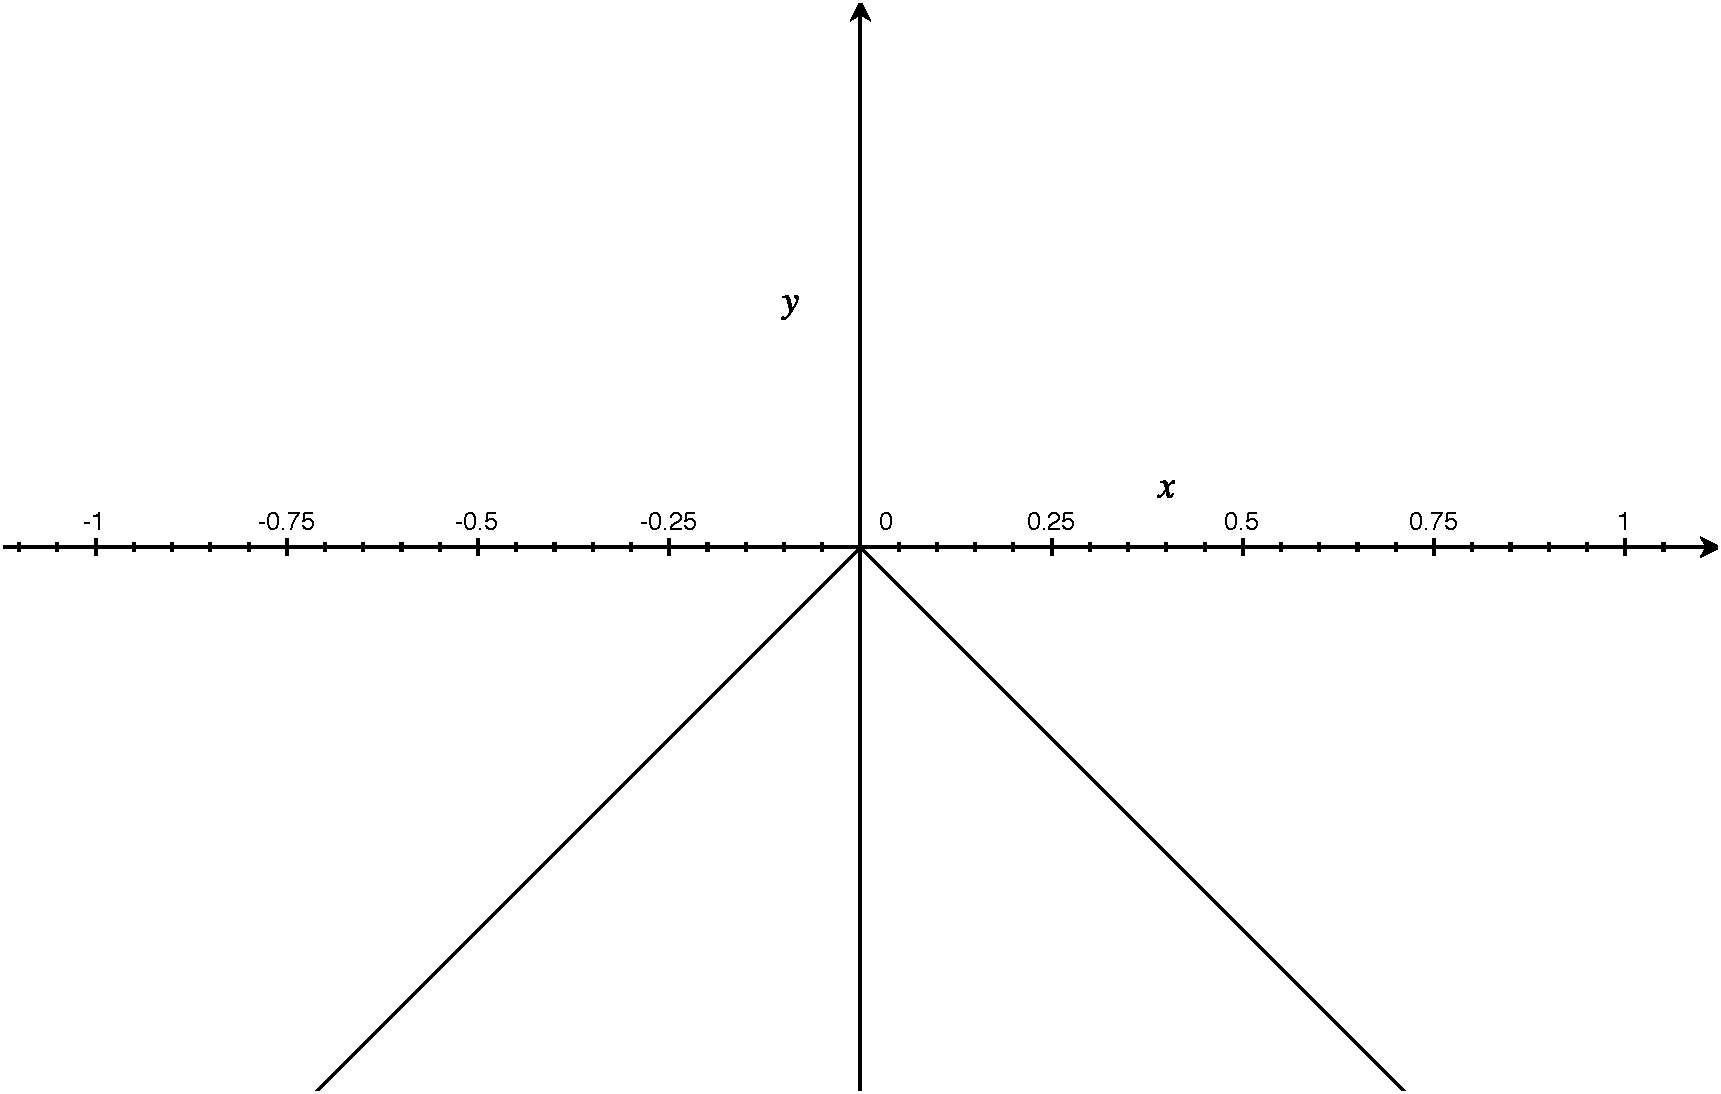
\includegraphics[width=2in]{./graphics/graphst2030201.pdf}
   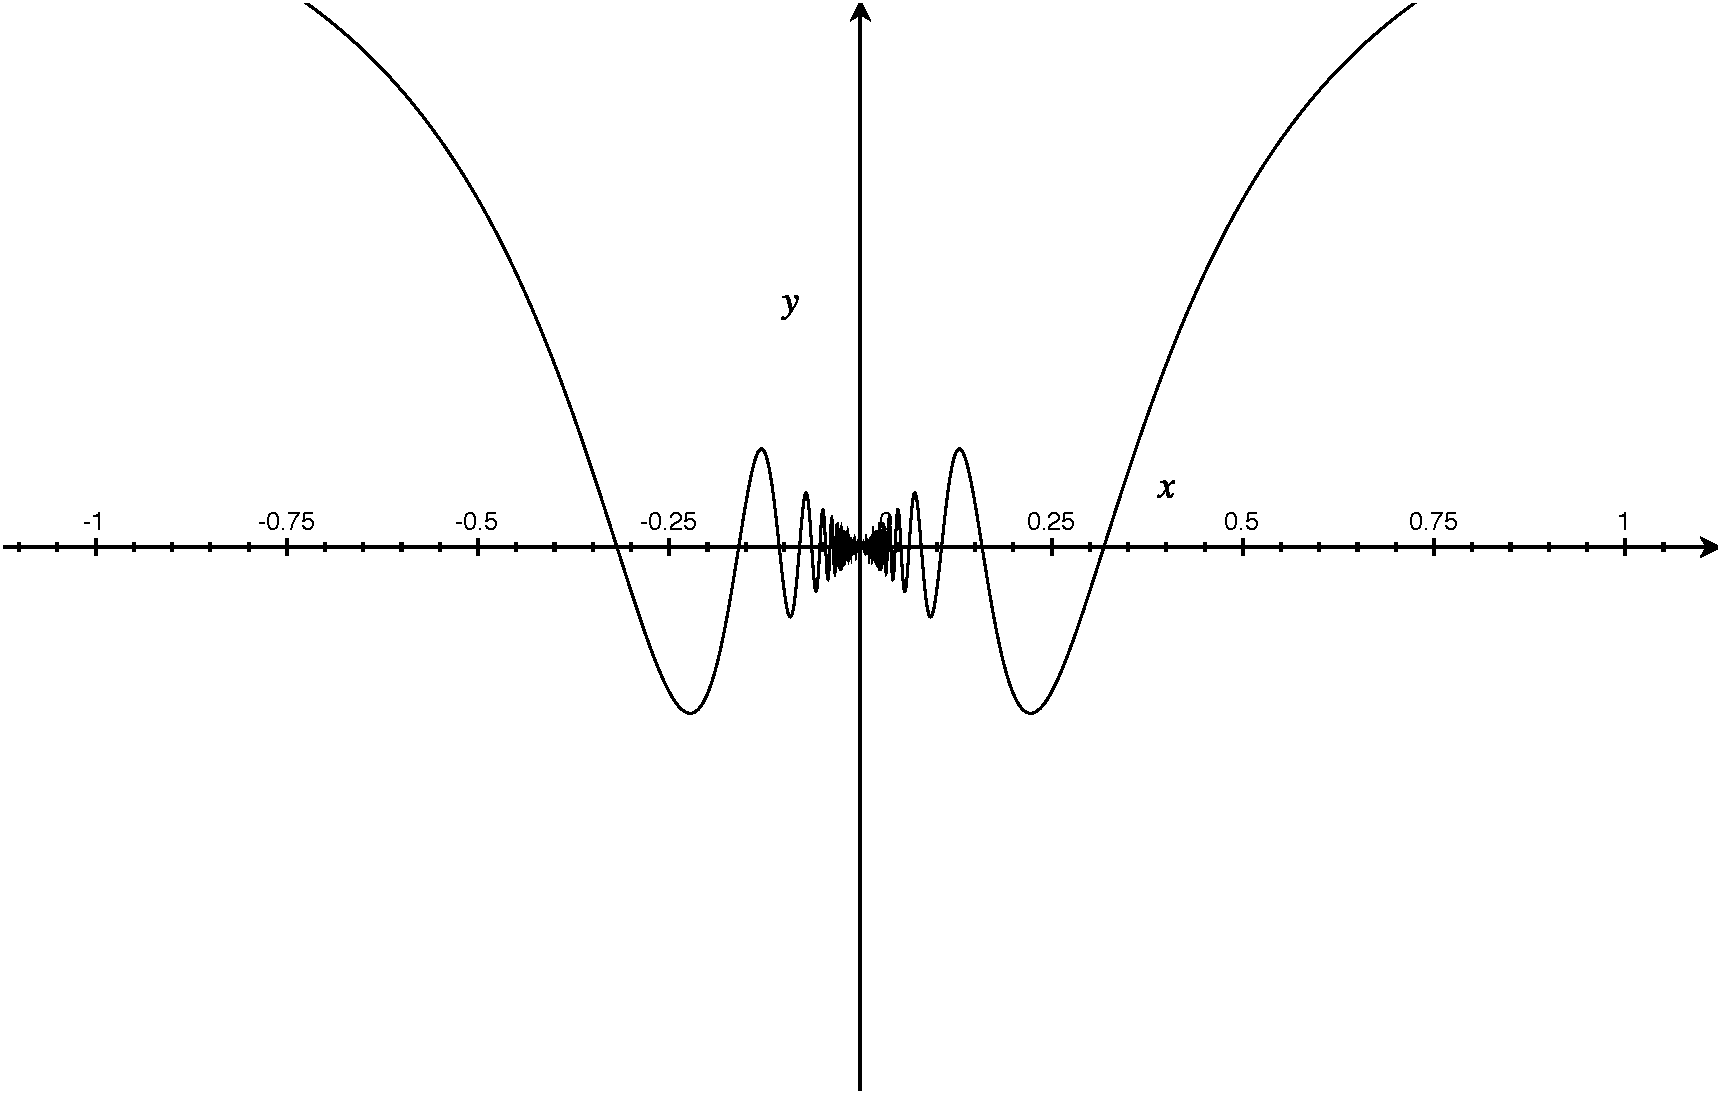
\includegraphics[width=2in]{./graphics/graphst20302.pdf}
   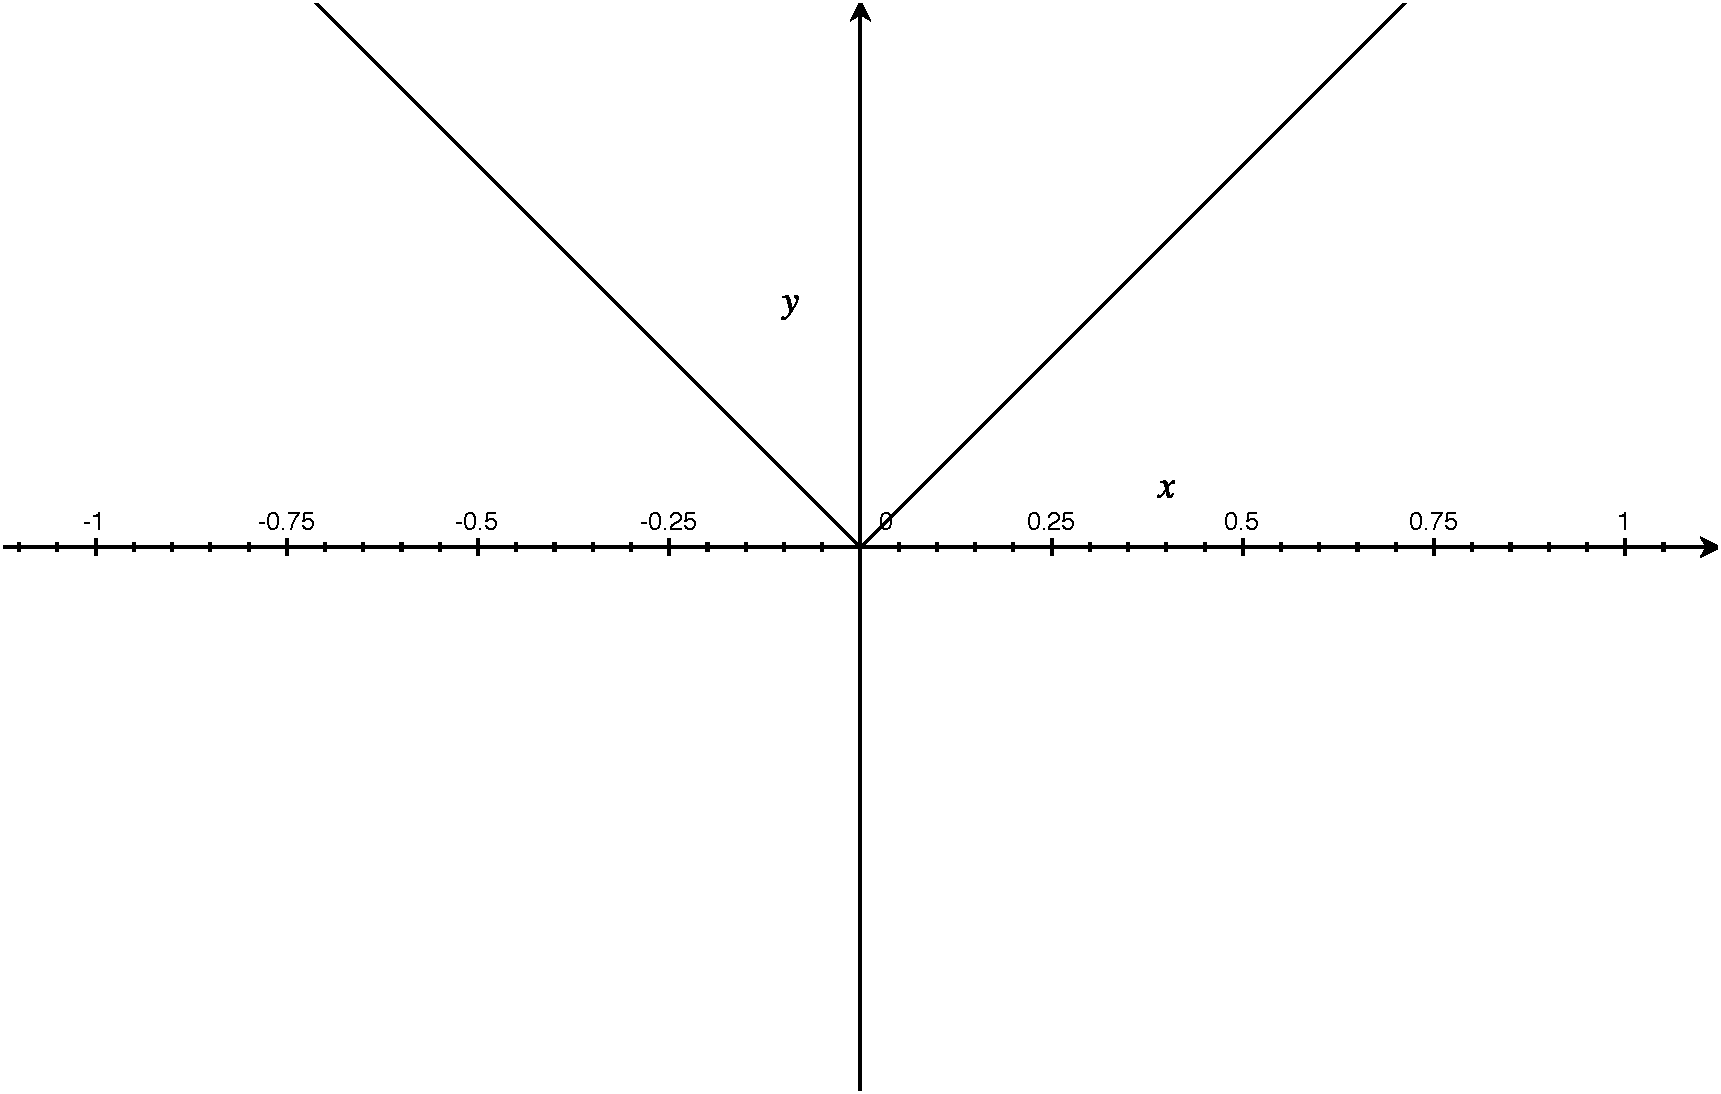
\includegraphics[width=2in]{./graphics/graphst20303.pdf}
  \caption{$y_1 = - \left| x \right|$,  $y_2 =  \displaystyle x \sin \left( \frac{1}{x} \right)$ and $y_3= \left| x \right|$. Note that $y_1 \leq y_2  \leq y_3$.}
   \label{fig:graphst02}
\end{figure}
\begin{solution}
We'll discuss this in class.

It's okay to use a calculator to make sure you're getting a squeeze. It's easy to get tricked!
\begin{eqnarray*}
-\left| x \right| \leq x \sin \left( \frac{1}{x} \right) \leq \left| x \right|
\end{eqnarray*}
You should graph (Figure \ref{fig:graphst02}, page \pageref{fig:graphst02}) these three functions to see that the inequality holds for all $x \neq 0$. Yes, it's tricky. Other squeezes exists, just be sure to graph them out.
\begin{eqnarray*}
\lim_{x \to 0} -\left| x \right| &=& 0\\ 
\lim_{x \to 0} \left| x\right| &=& 0
\end{eqnarray*}
By the ST,
\[
\mathop {\lim }\limits_{x \to 0}  x \sin \left( \frac{1}{x} \right) =0
\]
\end{solution}

\question Evaluate.
\[
\mathop {\lim }\limits_{x \to 0^+}  \frac{x^2}{\csc^2 x}
\]

\begin{solution}
We'll discuss this in class.

\begin{eqnarray*}
\lim_{x \to 0^+}  \frac{x^2}{\csc^2 x} &=& \lim_{x \to 0^+}  x^2 \sin^2 x = 0
\end{eqnarray*}

\end{solution}

\end{questions}








 




\subsection{Assignment}
You should read \S  2.6 and do the WebAssign assignment mth.122.06.06.
\vfill
\pagebreak
%*-*-*-*-*-*-*-*-*-*-*-*-*-*-*-*-*-*-*-*-*-*-*-*-*-*-*-*-*-*-*-*-*-*-*-*-*-*-*-*-*-*-*-*-*-*-*-*-*-*-*-*-*-*-*-*-*-*-*-*-*-*-*-*-*-*-*-*-*-*-*-*-*-*-*-*-*-*-*-*-*-*-*-*-

\begin{teacher}
\subsection{Assessments}
The following questions are related to the WebAssign assignments and may be used to assess students' ability. Please do not share any of these questions with students.
\begin{questions}
	
\question 	%RogaCalcET2 2.6.002	WA-1701522

Problem 2 \S2.6.
\begin{solution}
\end{solution}

\question 	%RogaCalcET2 2.6.003	WA-1739561

Problem 3 \S2.6.
\begin{solution}
\end{solution}

\question 	%RogaCalcET2 2.6.006	WA-1689413

Problem 6 \S2.6.
\begin{solution}

\end{solution}

\question 	%RogaCalcET2 2.6.007	WA-1701732

Use the Squeeze Theorem to evaluate the limit.
\[
\lim_{x \to 0} x \cos \frac{5}{x}
\]
\begin{solution}

\end{solution}

\question 	%RogaCalcET2 2.6.010	WA-1718606

Use the Squeeze Theorem to evaluate the limit.
\[
\lim_{x \to 3} \left(x^2 - 9\right) \frac{x - 3}{\left|x - 3\right|}
\]
\begin{solution}

\end{solution}

\question 	%RogaCalcET2 2.6.018	WA-1718960

Evaluate the limit using Theorem 2\footnote{\[ \lim_{\theta \to 0} \frac{\sin \theta}{\theta} =1, \quad \lim_{\theta \to 0} \frac{1 - \cos \theta}{\theta} =0 \]} as necessary.
\[
\lim_{x \to 0} \frac{\sin 8x \sec 7x}{5x}
\]
\begin{solution}

\end{solution}


\question 	%RogaCalcET2 2.6.020	WA-1701507

Evaluate the limit using Theorem 2\footnote{\[ \lim_{\theta \to 0} \frac{\sin \theta}{\theta} =1, \quad \lim_{\theta \to 0} \frac{1 - \cos \theta}{\theta} =0 \]} as necessary.
\[
\lim_{t \to 0} \frac{\sin^2 5t}{t}
\]
\begin{solution}

\end{solution}

\question 	%RogaCalcET2 2.6.021	WA-1701632

Evaluate the limit using Theorem 2\footnote{\[ \lim_{\theta \to 0} \frac{\sin \theta}{\theta} =1, \quad \lim_{\theta \to 0} \frac{1 - \cos \theta}{\theta} =0 \]} as necessary.
\[
\lim_{x \to 0} \frac{x^2}{\sin^2 3x}
\]
\begin{solution}

\end{solution}

\question 	%RogaCalcET2 2.6.022	WA-1701572

Evaluate the limit using Theorem 2\footnote{\[ \lim_{\theta \to 0} \frac{\sin \theta}{\theta} =1, \quad \lim_{\theta \to 0} \frac{1 - \cos \theta}{\theta} =0 \]} as necessary.
\[
\lim_{x \to \pi/2} \frac{1 - 9 \cos x}{4x}
\]
\begin{solution}

\end{solution}

\question 	%RogaCalcET2 2.6.027	WA-1701679

Evaluate the limit.
\[
\lim_{x \to 0} \frac{\sin 2x}{x}
\]
\begin{solution}

\end{solution}

\question 	%RogaCalcET2 2.6.028	WA-1739502

Evaluate the given limit using the hint given below.\footnote{\[\frac{\sin Ax}{\sin Bx} = \frac{A}{B} \cdot \frac{\sin Ax}{Ax} \cdot \frac{Bx}{\sin Bx} \]}
\[
\lim_{h \to 0} \frac{\sin 2 h}{\sin 7 h}
\]
\begin{solution}

\end{solution}


\question 	%RogaCalcET2 2.6.049	WA-1711513

Evaluate the limit.
\[
\lim_{x \to 0} \frac{\tan 7x}{2x}
\]
\begin{solution}

\end{solution}

\question 	%RogaCalcET2 2.6.034	WA-1701613

Evaluate the limits.
\begin{align*}
\lim_{x \to 0^+} \frac{\sin 10x}{\left| 10 x \right|} &=\\[10pt]
\lim_{x \to 0^-} \frac{\sin 10x}{\left| 10 x \right|} &=
\end{align*}
\begin{solution}

\end{solution}

\question 	%RogaCalcET2 2.6.053	WA-1718953

Use the identity
\[
\lim_{x \to 0} \frac{1 - \cos x}{x^2} = \frac{1}{2}
\]
to evaluate the following limit.
\[
\lim_{x \to 0} \frac{\cos 2x - 1}{6x^2}
\]
\begin{solution}

\end{solution}

\question 	%RogaCalcET2 2.6.055	WA-1733778

Use the value
\[
\lim_{x \to 0} \frac{1 - \cos x}{x^2} = \frac{1}{2}
\]
to evaluate the following limits.
\begin{align*}
\lim_{x \to 0^+} \frac{\sqrt{3 - 3 \cos x}}{2x} &=\\[10pt]
\lim_{x \to 0^-} \frac{\sqrt{3 - 3 \cos x}}{2x} &=\\
\end{align*}
\begin{solution}

\end{solution}
\end{questions}
\end{teacher}
\vfill
\pagebreak

%*-*-*-*-*-*-*-*-*-*-*-*-*-*-*-*-*-*-*-*-*-*-*-*-*-*-*-*-*-*-*-*-*-*-*-*-*-*-*-*-*-*-*-*-*-*-*-*-*-*-*-*-*-*-*-*-*-*-*-*-*-*-*-*-*-*-*-*-*-*-*-*-*-*-*-*-*-*-*-*-*-*-*-*-
\section{mth.121.02.07}
\subsection{Calculating Limits at Infinity}



\subsubsection{Review}
Although initially difficult to grasp,
\[
\mathop {\lim }\limits_{x \to a}  f \left( x \right),
\]
this notation basically tells us to get close to $a$ (BUT DO NOT TOUCH $a$!). In a way, we are deifying $a$. Fact is, when you tell someone of a forbidden fruit, they want to touch it. But be warned, try not to touch it! If this notation says anything, it says, ``do not touch $a$, but please try to get close to $a$. As close as you like!'' Since $a$ exist on a one dimensional number line, you should note that there are two ways to approach any finite $a$.



We write
\[
\mathop {\lim }\limits_{x \to a^- }  f \left( x \right) = L
\]
and say that the \textbf{left-hand limit} of $f \left( x \right)$ as $x$ approaches $a$ is equal to $L$. A left hand limit just means that we are approaching $a$ from the left, or from values smaller than $a$. We can also write
\[
\mathop {\lim }\limits_{x \to a^+ }  f \left( x \right) = L
\]
and say that the \textbf{right-hand limit} of $f \left( x \right)$ as $x$ approaches $a$ is equal to $L$. A right hand limit just means that we are approaching $a$ from the right, or from values larger than $a$. For the limit
\[
\mathop {\lim }\limits_{x \to a }  f \left( x \right)
\]
to exist, both the left and right limits must exist and be the same. That is
\[
\mathop {\lim }\limits_{x \to a }  f \left( x \right) = L \quad \mbox{if and only if} \quad \mathop {\lim }\limits_{x \to a^- }  f \left( x \right) = L \quad \mbox{and} \quad \mathop {\lim }\limits_{x \to a^+ }  f \left( x \right) = L
\]
You should note that $L$ is referring to a single finite number. If $L$ is not finite, we say the limit does not exists. However,  mathematicians accept the following definitions.
\begin{description}
\item[$L \rightarrow \infty$:] Let $f$ be a function defined on both sides of $a$, except possibly at $a$ itself. Then
\[
\mathop {\lim }\limits_{x \to a }  f \left( x \right) = \infty
\]
means that the value of $f\left(x\right)$ can be made arbitrarily large (as large as we please) by taking $x$ sufficiently close to $a$, but not equal to $a$.
\item[$L \rightarrow  -\infty$:] Let $f$ be a function defined on both sides of $a$, except possibly at $a$ itself. Then
\[
\mathop {\lim }\limits_{x \to a }  f \left( x \right) = -\infty
\]
means that the value of $f\left(x\right)$ can be made arbitrarily large negative by taking $x$ sufficiently close to $a$, but not equal to $a$.
\end{description}



We can also allow $x$ to approach $\pm \infty$, basically to analyze a function's behavior in the extremes of infinity. The definition is: let $f$ be a function defined on some interval $\left( a, \ \infty \right)$. Then
\[
\mathop {\lim }\limits_{x \to \infty }  f \left( x \right) = L
\]
means that the values of $f$ can be made arbitrarily close to $L$ by taking $x$ sufficiently large.



We can also go in the other direction towards $-\infty$. The definition is: let $f$ be a function defined on some interval $\left( -\infty, \ a \right)$. Then
\[
\mathop {\lim }\limits_{x \to -\infty }  f \left( x \right) = L
\]
means that the values of $f$ can be made arbitrarily close to $L$ by taking $x$ sufficiently large negative.



\subsubsection{More Review}
Limits are discussed\footnote{Most teachers, and certainly most textbooks.} in MTH 119 (pre-calculus), I'll assume that you've had some practice with these limits and know that they are useful when graphing rational functions. Let's do an example to jog your memory.


\textbf{Example:} Given
\[
f \left( x \right) = \frac{x^2-3x+2}{2x^2+5x+3} = \frac{\left(x-1\right)\left(x-2\right)}{\left(2x+3\right)\left(x+1\right)},
\]
answer the following questions:

\begin{questions}
\question $x$-intercepts in point form.

\begin{solution}
By now this should seem very easy to do, especially considering how the function is presented in factored form.

\[
\left(1, \ 0 \right); \left(2, \ 0 \right)
\]
\end{solution}



\question $y$-intercept in point form.

\begin{solution}
Again, this should be very easy to do.

\[\left(0, \ \frac{2}{3} \right)
\]
\end{solution}



\question Equation of the horizontal asymptote.

\begin{solution}
This will be discussed in class.

\[
y = \frac{1}{2}
\]
\end{solution}



\question Equation of the vertical asymptotes.

\begin{solution}
This will be discussed in class.

\[
x = -1; \quad x = -\frac{3}{2}
\]
\end{solution}


\item Graph $f\left( x \right)$ using the above information and sign analysis.
\begin{solution}
Your graph (Figure \ref{fig:graph0740}, page \pageref{fig:graph0740}) should contain similar details.
\end{solution}
\begin{figure}[htbp]
   \centering
   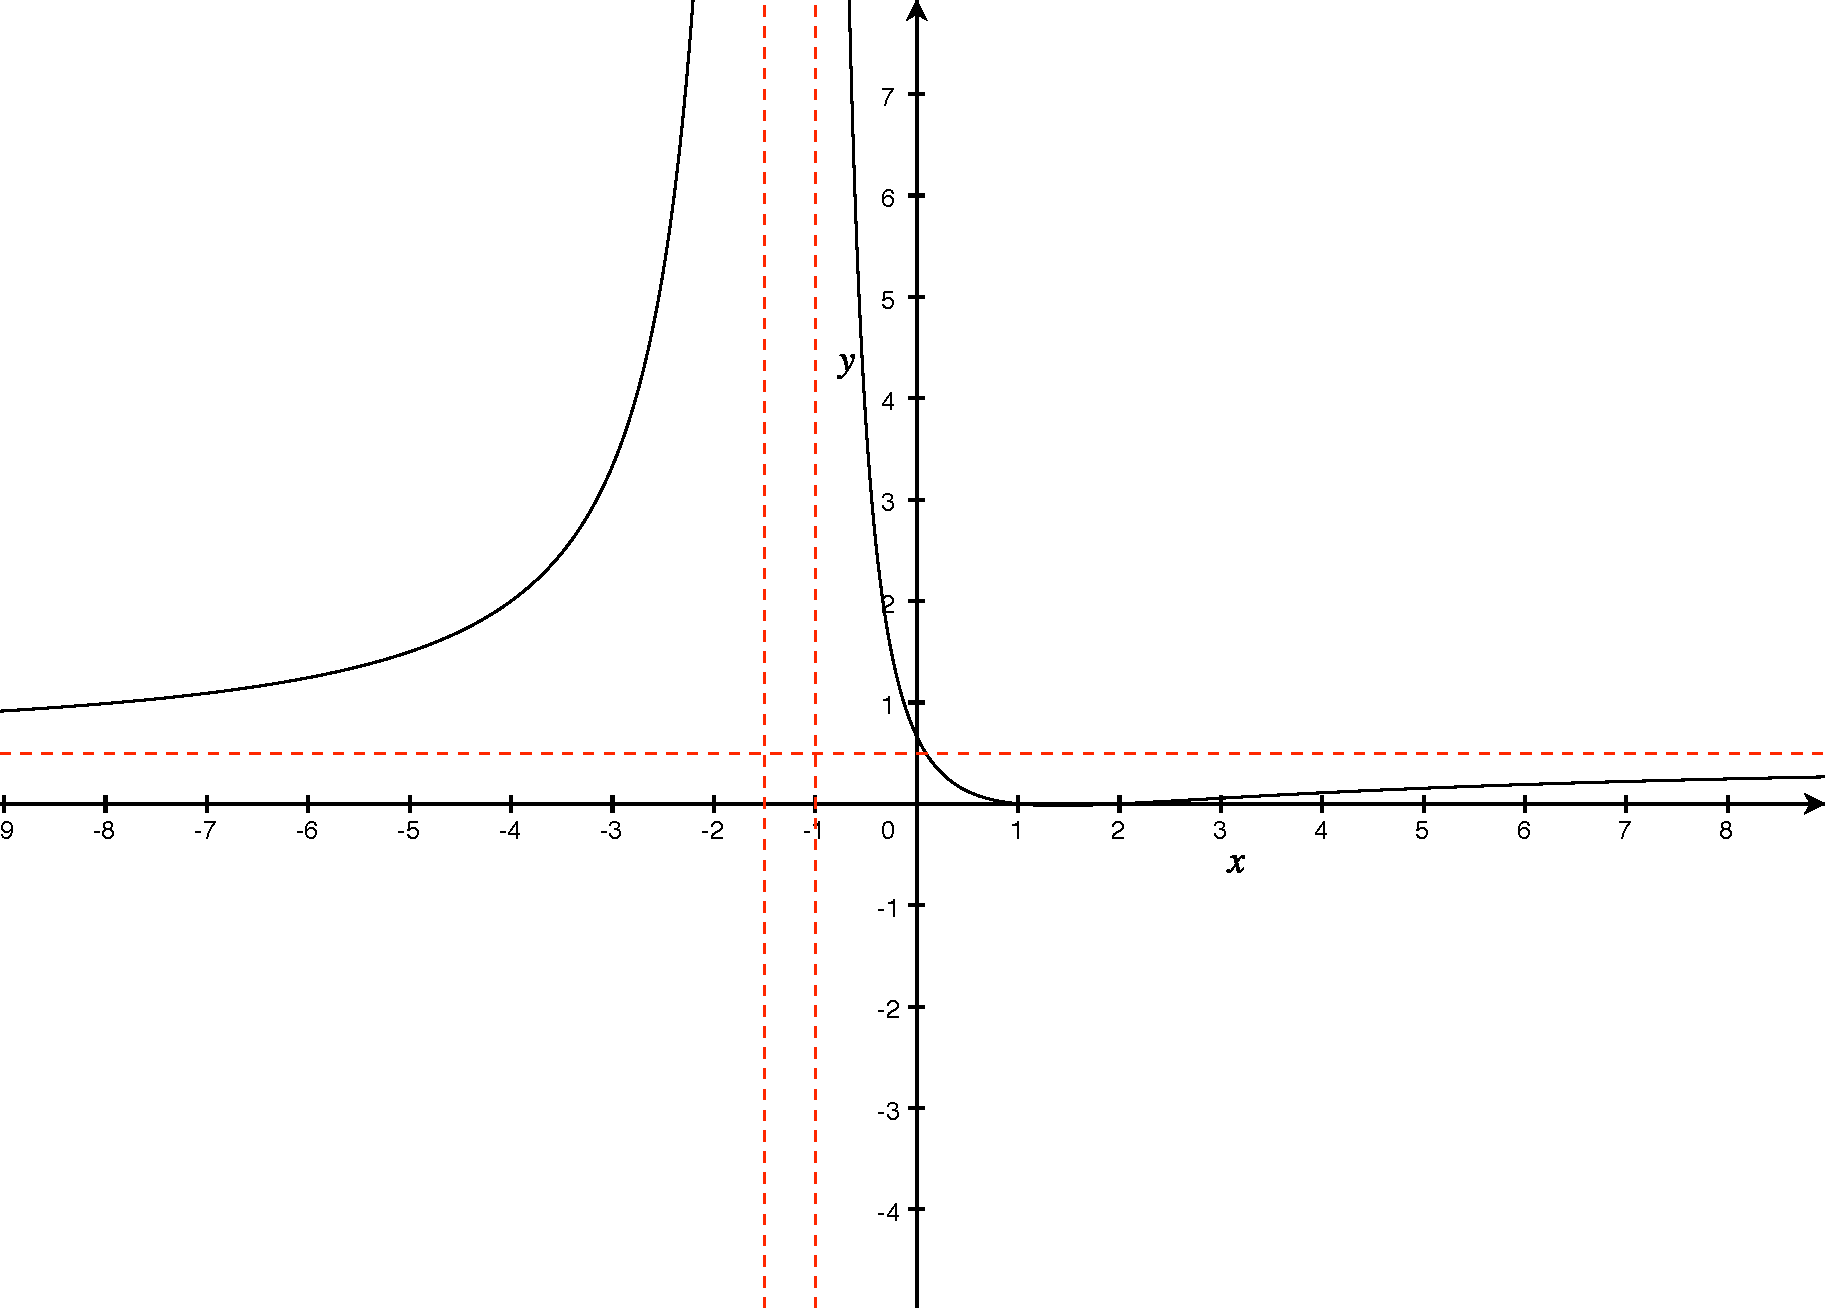
\includegraphics[width=.6\textwidth]{graphics/graph0740.pdf} 
   \caption{Partial graph of $f \left( x \right)$.}
   \label{fig:graph0740}
\end{figure}
\end{questions}



\textbf{Example:} Now let's take a careful look at:
\[
g\left( x \right) = \frac{5x^2\left(x-1\right)}{\left(x-1\right)\left(3x-2\right)\left(x+2\right)}
\]

\begin{figure}[htbp]
   \centering
   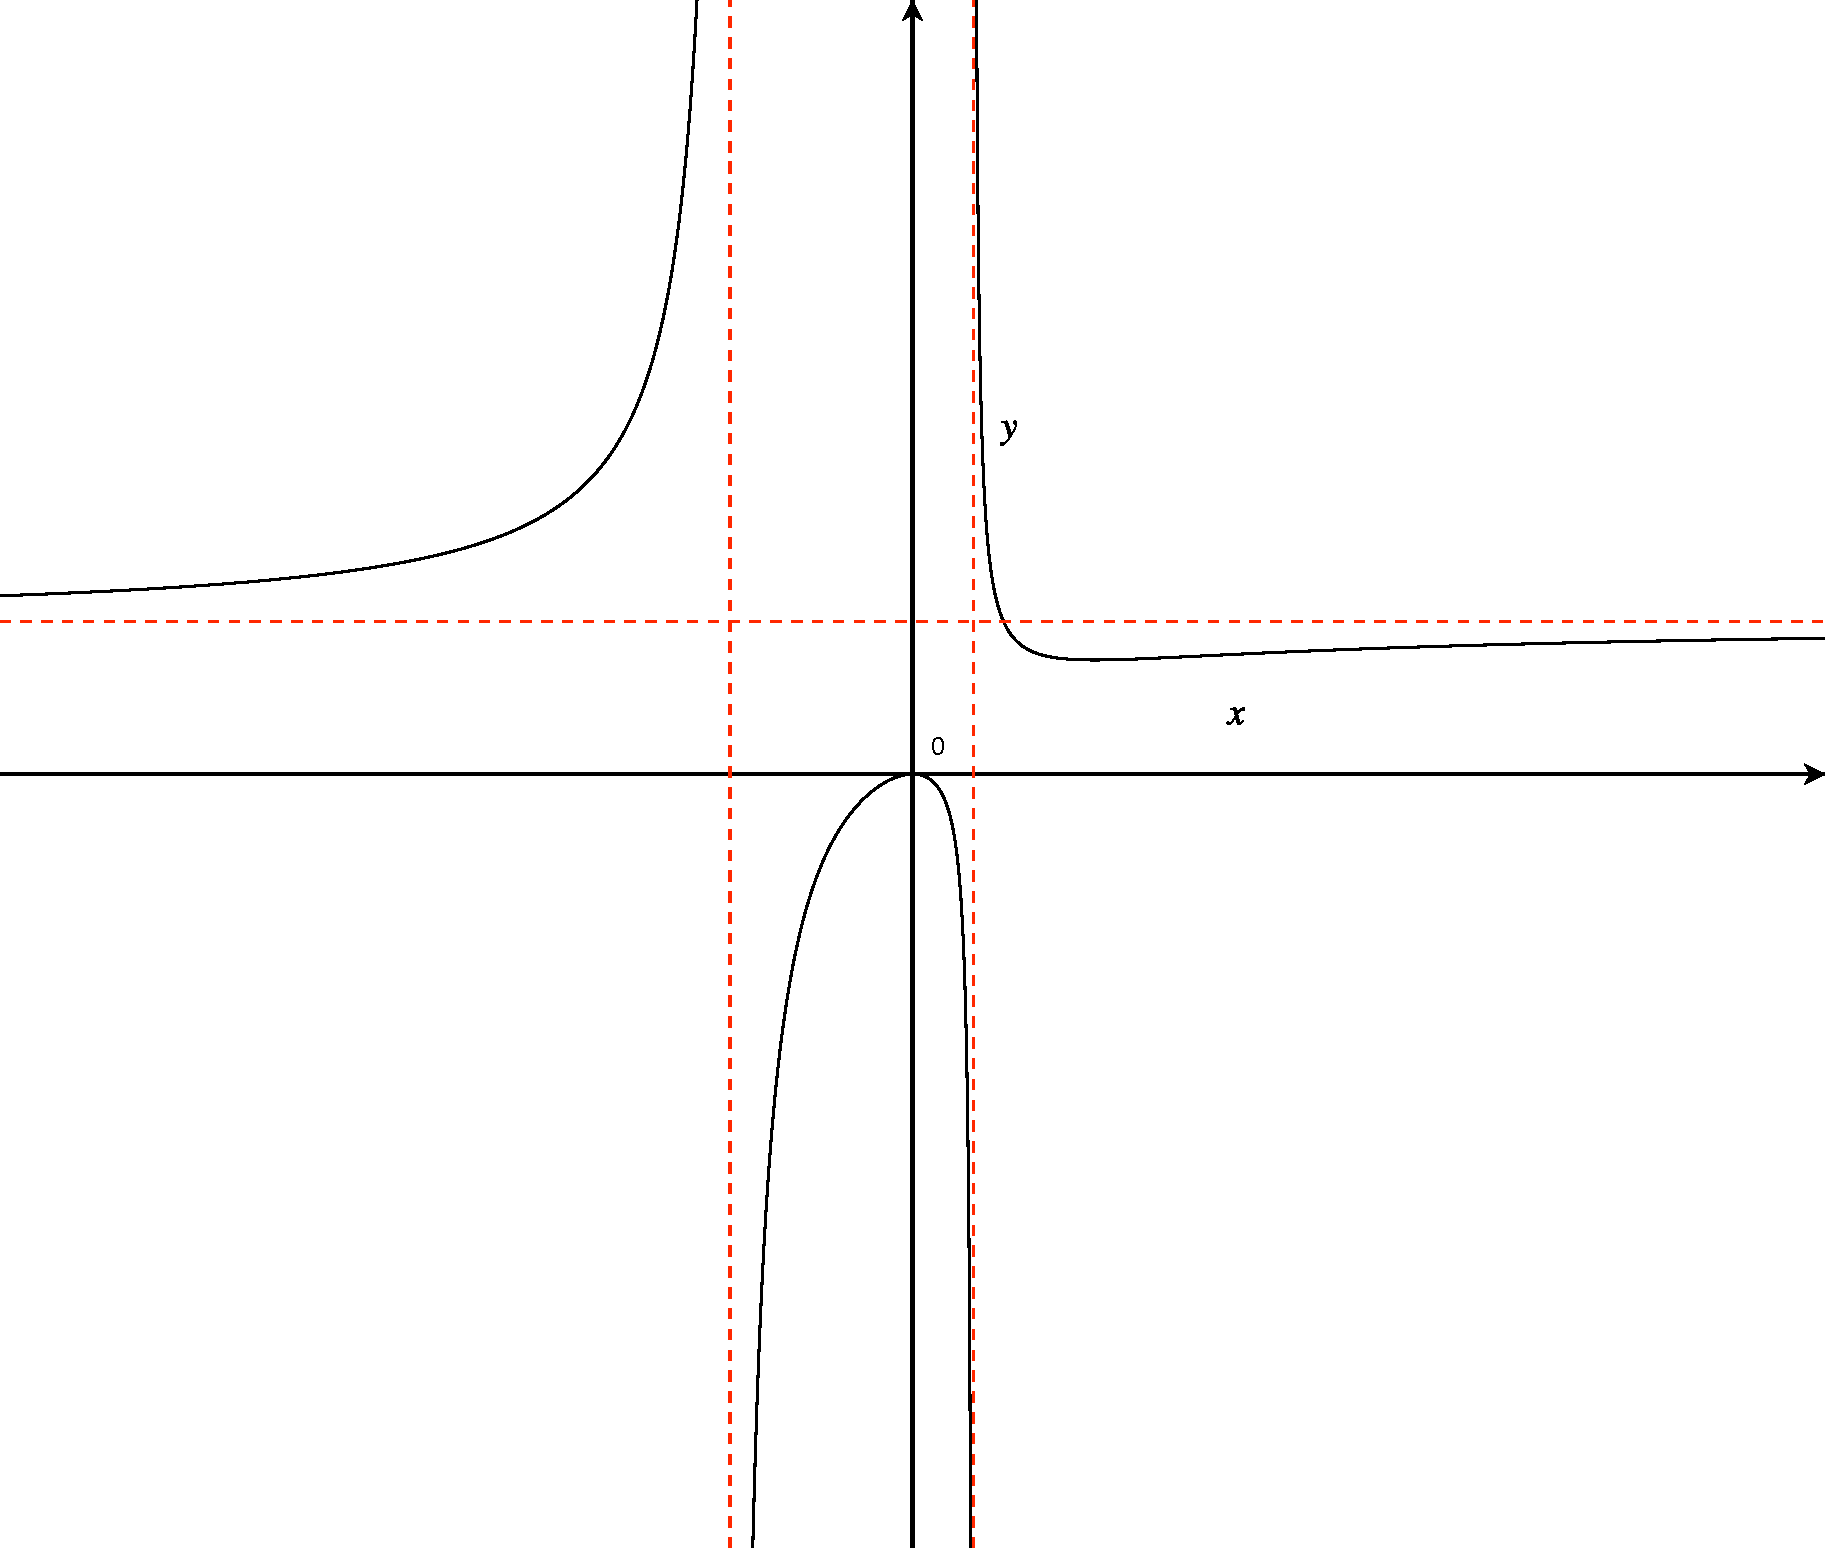
\includegraphics[width=.6\textwidth]{./graphics/graph0750.pdf} 
   \caption{Partial graph of $g \left( x \right)$, properly scaled, but no units given.}
   \label{fig:graph5007}
\end{figure}


Here are some relevant questions.
\begin{questions}
\question $\displaystyle \mathop {\lim }\limits_{x \to -\infty }  g \left( x \right) = $
\begin{solution}
This will be discussed in class.

\[
\lim_{x \to +\infty }  g \left( x \right) = \frac{5}{3}
\]
\end{solution}


\question $\displaystyle \mathop {\lim }\limits_{x \to +\infty }  g \left( x \right) = $
\begin{solution}
This will be discussed in class.

\[
\lim_{x \to +\infty }  g \left( x \right) = \frac{5}{3}
\]
\end{solution}


\question $\displaystyle \mathop {\lim }\limits_{x \to 1^+ }  g \left( x \right) = $
\begin{solution}
This will be discussed in class.

\[
\lim_{x \to 1^+ }  g \left( x \right) = \frac{5}{3}
\]
\end{solution}


\question $\displaystyle \mathop {\lim }\limits_{x \to 1^- }  g \left( x \right) = $
\begin{solution}
This will be discussed in class.

\[
\lim_{x \to 1^+ }  g \left( x \right) = \frac{5}{3}
\]
\end{solution}


\question $\displaystyle \mathop {\lim }\limits_{x \to 1 }  g \left( x \right) = $
\begin{solution}
This will be discussed in class.

\[
\lim_{x \to 1^+ }  g \left( x \right) = \frac{5}{3}
\]
\end{solution}


\question $\displaystyle g \left( 1 \right) = $
\begin{solution}
This will be discussed in class.

Undefined.
\end{solution}


\question Determine and evaluate the other limits that we should look at.
\begin{solution}
This will be discussed in class.

\begin{eqnarray*}
\lim_{x \to -2^+ }  g \left( x \right) &=& -\infty \\
\lim_{x \to -2^- }  g \left( x \right) &=& \infty \\
\lim_{x \to \frac{2}{3}^+ }  g \left( x \right) &=&  \infty \\
\lim_{x \to \frac{2}{3}^- }  g \left( x \right) &=& -\infty 
\end{eqnarray*}
\end{solution}


\end{questions}
 
 
\subsection{Examples}
\begin{questions}
\question Evaluate.
\[
\lim_{x \to \infty} \frac{9x^2-3x+4}{5-3x-11x^2}
\]

\begin{solution}
We'll discuss this in class.

\[
\lim_{x \to \infty} \frac{9x^2-3x+4}{5-3x-11x^2} = -\frac{9}{11}
\]
\end{solution}

\question Evaluate.
\[
\lim_{x \to \infty} \frac{4x-3}{\sqrt{25x^2+4x}}
\]

\begin{solution}
We'll discuss this in class.

\[
\lim_{x \to \infty} \frac{4x-3}{\sqrt{25x^2+4x}} = \frac{4}{5}
\]
\end{solution}


\question Evaluate.
\[
\lim_{x \to -\infty} \frac{4x-3}{\sqrt{25x^2+4x}}
\]

\begin{solution}
We'll discuss this in class.

\[
\lim_{x \to -\infty} \frac{4x-3}{\sqrt{25x^2+4x}} = -\frac{4}{5}
\]
\end{solution}


\question Evaluate.
\[
\lim_{x \to \infty} \left( 2\sqrt{x} - \sqrt{x+2} \right)
\]

\begin{solution}
We'll discuss this in class.

\[
\lim_{x \to \infty} \left( 2\sqrt{x} - \sqrt{x+2} \right) = \infty
\]
\end{solution}


\question Evaluate.
\[
\lim_{x \to \infty} \arctan \left( \frac{1+x}{1-x}\right)
\]

\begin{solution}
We'll discuss this in class.

\[
\lim_{x \to \infty} \arctan \left( \frac{1+x}{1-x}\right) = - \frac{\pi}{4}
\]
\end{solution}


\question Evaluate.
\[
\lim_{x \to \infty}  \left( \frac{1}{x} - \frac{1}{x+2}\right)
\]

\begin{solution}
We'll discuss this in class.

\[
\lim_{x \to \infty}  \left( \frac{1}{x} - \frac{1}{x+2}\right) = 0
\]
\end{solution}


\question Evaluate.
\[
\lim_{x \to -\infty} \frac{\left| x \right| + x}{x+1}
\]

\begin{solution}
We'll discuss this in class.

\[
\lim_{x \to -\infty} \frac{\left| x \right| + x}{x+1} = 0
\]
\end{solution}

\question Evaluate.
\[
\lim_{x \to \infty} \frac{\left| x \right| + x}{x+1}
\]

\begin{solution}
We'll discuss this in class.

\[
\lim_{x \to \infty} \frac{\left| x \right| + x}{x+1}  = 2
\]
\end{solution}

\end{questions}











\subsection{Assignment}
You should read \S  2.7 and do the WebAssign assignment mth.121.02.07.
\vfill
\pagebreak
%*-*-*-*-*-*-*-*-*-*-*-*-*-*-*-*-*-*-*-*-*-*-*-*-*-*-*-*-*-*-*-*-*-*-*-*-*-*-*-*-*-*-*-*-*-*-*-*-*-*-*-*-*-*-*-*-*-*-*-*-*-*-*-*-*-*-*-*-*-*-*-*-*-*-*-*-*-*-*-*-*-*-*-*-

\begin{teacher}
\subsection{Assessments}
The following questions are related to the WebAssign assignments and may be used to assess students' ability. Please do not share any of these questions with students.
\begin{questions}		
\question 	%RogaCalcET2 2.7.007	WA-1733780

Evaluate the limit.
\[
\lim_{x \to \infty} \frac{4x}{9x+9}
\]
\begin{solution}
Work.
\end{solution}


\question 	%RogaCalcET2 2.7.009	WA-1718958

Evaluate the limit.
\[
\lim_{x \to \infty} \frac{2x^2+8x}{4x^4+3x^3-29}
\]
\begin{solution}
Work.
\end{solution}

\question 	%RogaCalcET2 2.7.010	WA-1718988

Evaluate the limit.
\[
\lim_{x \to \infty} \frac{4x+6}{3}
\]
\begin{solution}
Work.
\end{solution}

\question 	%RogaCalcET2 2.7.012	WA-1718976

Evaluate the limit.
\[
\lim_{x \to \infty} \frac{7x^2-5}{6-29x}
\]
\begin{solution}
Work.
\end{solution}

\question 	%RogaCalcET2 2.7.019	WA-1725174

Find the horizontal asymptotes (there's two).
\[
f\left(x\right) = \frac{\sqrt{6x^2 + 7}}{9x+4} 
\]
\begin{solution}
Work.
\end{solution}


\question 	%RogaCalcET2 2.7.021	WA-1725155

Find the horizontal asymptote.
\[
f\left(x\right) = \frac{3e^x}{1 + e^{-x}}
\]
\begin{solution}
Work.
\end{solution}

\question 	%RogaCalcET2 2.7.022	WA-1725196

Find the horizontal asymptotes (there's two).
\[
f\left(x\right) = \frac{9x^{1/3}}{\left(64x^2+10\right)^{1/6}} 
\]
\begin{solution}
Work.
\end{solution}

\question 	%RogaCalcET2 2.7.025	WA-1725159


Evaluate the limit.
\[
\lim_{x \to -\infty} \frac{x^2+7x^{1/3}}{\sqrt{16x^4+6}} 
\]
\begin{solution}
Work.
\end{solution}

\question 	%RogaCalcET2 2.7.026	WA-1725187

Evaluate the limit.
\[
\lim_{x \to -\infty} \frac{6x-4}{\sqrt{4x^2+5}} 
\]
\begin{solution}
Work.
\end{solution}

\question 	%RogaCalcET2 2.7.031	WA-1725161

Evaluate the limit.
\[
\lim_{x \to \infty} 6 \arctan \frac{x}{7}
\]
\begin{solution}
Work.
\end{solution}


\question 	%RogaCalcET2 2.7.038	WA-1725212

Calculate the limit.
\[
\lim_{x \to \infty} \left( \frac{1}{x} - \frac{9x}{x+2} \right)
\]

\begin{solution}
Work.
\end{solution}


\question 	%RogaCalcET2 2.7.039	WA-1725154

Calculate the limit.
\[
\lim_{x \to \infty} \left[ \ln \left( 5x+1\right) - \ln \left( 2x+1 \right) \right]
\]
\begin{solution}
Work.
\end{solution}




\question 	%RogaCalcET2 2.7.040	WA-1725183

Calculate the limit.
\[
\lim_{x \to \infty} \left( \ln \sqrt{5x^4+2} - \ln x \right) 
\]
\begin{solution}
Work.
\end{solution}

\question 	%RogaCalcET2 2.7.041	WA-1725144

Calculate the limit.
\[
\lim_{x \to \infty} \arctan \left( \frac{x^2+5}{x+5} \right)
\]
\begin{solution}
Work.
\end{solution}


\question 	%RogaCalcET2 2.7.042	WA-1725204

Calculate the limit.
\[
\lim_{x \to \infty} \arctan \left( \frac{x+9}{x+3} \right)
\]
\begin{solution}
Work.
\end{solution}

\end{questions}

\end{teacher}
\vfill
\pagebreak

%*-*-*-*-*-*-*-*-*-*-*-*-*-*-*-*-*-*-*-*-*-*-*-*-*-*-*-*-*-*-*-*-*-*-*-*-*-*-*-*-*-*-*-*-*-*-*-*-*-*-*-*-*-*-*-*-*-*-*-*-*-*-*-*-*-*-*-*-*-*-*-*-*-*-*-*-*-*-*-*-*-*-*-*-
\section{mth.121.02.08}
\subsection{Intermediate Value Theorem}

Karl Weierstrass was a German mathematician who proved the Intermediate Value Theorem (IVT), which was not an easy task. Some have said that he proved the obvious, but it nonetheless had to be proved before it could become a theorem. In MTH-119 you used this theorem to show the existence of roots. Here's what the theorem states:
\begin{quote}
Suppose $f$ is continuous on the closed interval $\left[ a, \ b \right]$ and $W$ is any number between $f \left( a \right)$ and $f \left( b\right)$, where $f \left( a \right) \neq f \left( b \right)$. Then, there is a number $c \in \left( a, \ b \right)$ for which $f \left(c\right) = W$.
\end{quote}

\textbf{Example:} Suppose you're asked to show that
\[
f \left( x \right) = x^3 - 4x - 2,
\]
has a zero on the interval $\left[ -2, \ -1 \right]$.

\begin{solution}
Keep in mind that you're not being asked for the root, but rather its existence. In short use the IVT and state the following.
\begin{itemize}
\item $f \left( x \right)$ is continuous on $\left[ -2, \ -1 \right]$.
\item $f \left( -2 \right) = -2 < 0 < 1 = f \left( -1 \right)$
\item By the IVT there is a number $c \in \left( -2, \ -1 \right)$ for which $f \left(c\right) = 0 = W$
\end{itemize}
Here's a graph (Figure \ref{fig:graph0803}, page \pageref{fig:graph0803}) \emph{illustrating} the obvious.
\end{solution}
\begin{figure}[htbp] %  figure placement: here, top, bottom, or page
   \centering
   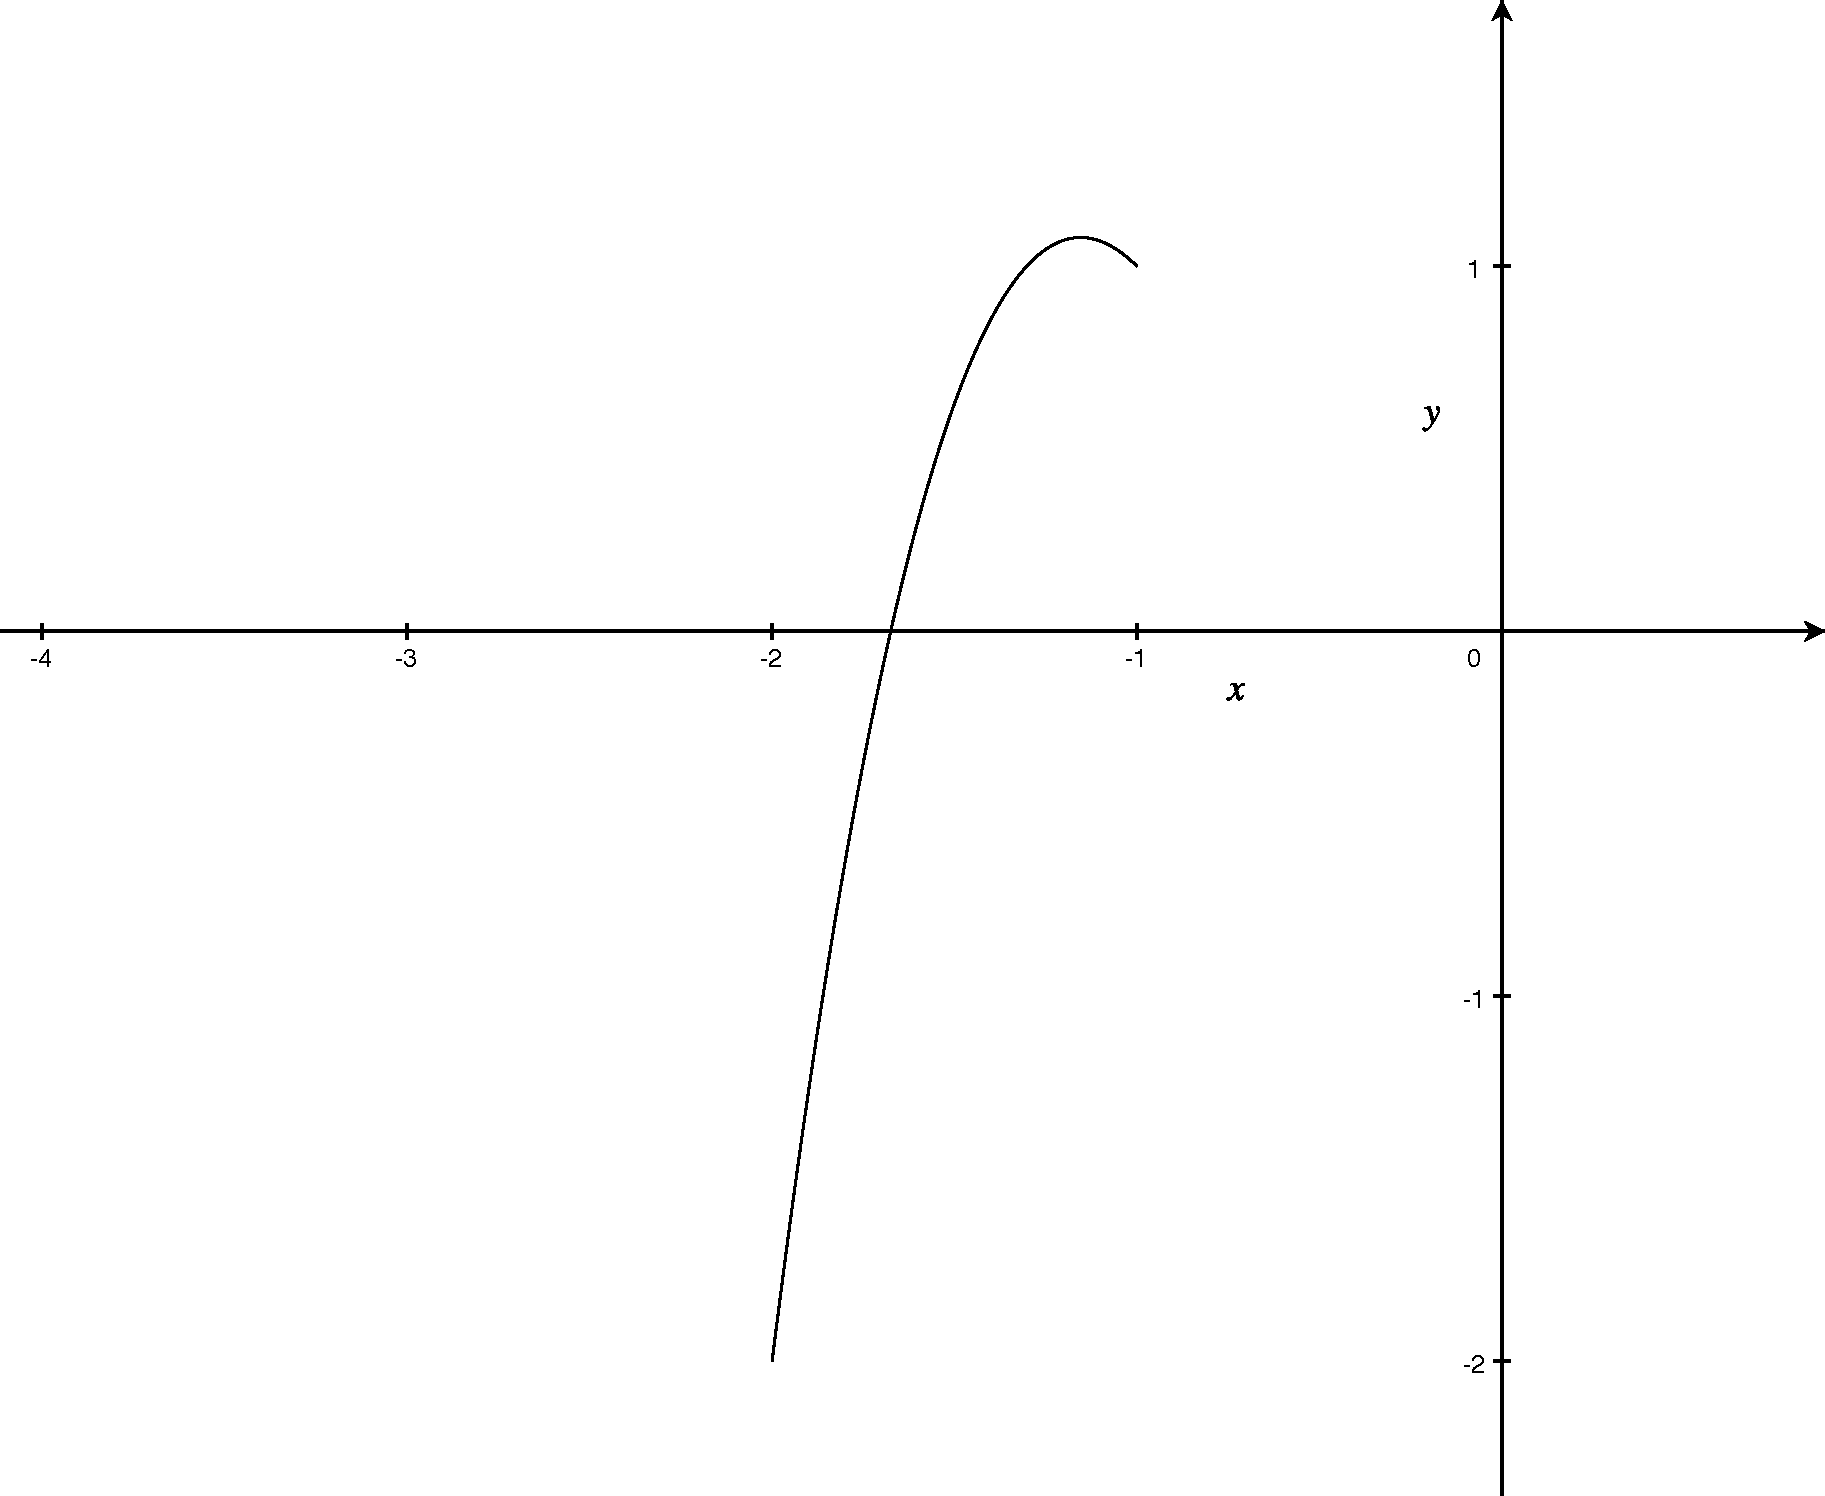
\includegraphics[width=3in]{./graphics/graph0803.pdf} 
   \caption{Graph of $f \left( x \right)= x^3 - 4x - 2$ on $\left[ -2, \ -1 \right]$.}
   \label{fig:graph0803}
\end{figure}
What's not obvious is the value of $c$, but I guess you can make a pretty good guess at what it is. Furthermore, you can use software to get a good approximation, possibly the exact answer.\footnote{My calculator returns $-1.67513087057$. Mathematica is able to compute three real roots exactly.}


\subsection{Examples}
\begin{questions}
\item Prove using the IVT, that
\[
\sqrt{x} + \sqrt{x+2}=3,
\]
has a solution. You may also solve\footnote{$x=49/36$} this equation for $x$ using methods learned in  algebra.

\begin{solution}
We'll discuss this in class.

Let's do this solving the equation for zero first and then letting this be our function.
\begin{eqnarray*}
\sqrt{x} + \sqrt{x+2}&=&3\\
\sqrt{x} + \sqrt{x+2} - 3 &=&0\\
f\left( x \right) &=& \sqrt{x} + \sqrt{x+2}-3
\end{eqnarray*}
\begin{itemize}
\item $f \left( x \right)$ is continuous on $\left[ 0, \ \infty \right)$.
\item $f \left( 0 \right)  < 0 <  f \left( 7 \right)$
\item By the IVT there is a number $c \in \left( 0, \ 7 \right)$ for which $f \left(c\right) = 0 = W$
\end{itemize}
\end{solution}



\question Prove using the IVT, that
\[
\arctan x = \arccos x,
\]
has a solution. If you're so inclined, try to use software\footnote{Visit \url{http://m10.mathography.org/} for more information about using software to solve difficult mathematical problems. Here, you'll see that
\[
x= \sqrt{\frac{\sqrt{5}-1}{2}}
\]
This can also be done using what you've learned in precalculus.} to solve this equation.

\begin{solution}
We'll discuss this in class.

Let's do this solving the equation for zero first and then letting this be our function.
\begin{eqnarray*}
\arctan x &=& \arccos x\\
\arctan x - \arccos x &=&0\\
f\left( x \right) &=& \arctan x - \arccos x
\end{eqnarray*}
You'll probably need a calculator for this one.
\begin{itemize}
\item $f \left( x \right)$ is continuous on $\left[ -1, \ 1 \right]$.
\item $f \left( -1 \right)  < 0 <  f \left( 1 \right)$
\item By the IVT there is a number $c \in \left( -1, \ 1 \right)$ for which $f \left(c\right) = 0 = W$
\end{itemize}
\end{solution}


\end{questions}






\subsection{Assignment}
You should read \S  2.8 and do the WebAssign assignment mth.121.02.08.

\vfill
\pagebreak

%*-*-*-*-*-*-*-*-*-*-*-*-*-*-*-*-*-*-*-*-*-*-*-*-*-*-*-*-*-*-*-*-*-*-*-*-*-*-*-*-*-*-*-*-*-*-*-*-*-*-*-*-*-*-*-*-*-*-*-*-*-*-*-*-*-*-*-*-*-*-*-*-*-*-*-*-*-*-*-*-*-*-*-*-

\begin{teacher}
\subsection{Assessments}
The following questions are related to the WebAssign assignments and may be used to assess students' ability. Please do not share any of these questions with students.
\begin{questions}		
\question 	%RogaCalcET2 2.8.004	WA-1711547

Using IVT, does the function
\[
f\left(x\right) = \frac{x^2}{x^7 + 5}
\]
have the value $0.172$ for some $x$ in $\left[0, \ 1 \right]$?

\begin{solution}
Work
\end{solution}

\question 	%RogaCalcET2 2.8.003	WA-1711542

Using IVT, does the function
\[
f\left(x\right) = x^2 \tan x
\]
have the value $0.032$ for some $x$ in $\left[0, \ \pi/8 \right]$?

\begin{solution}
Work
\end{solution}

\question 	%RogaCalcET2 2.8.013	WA-1725195

Using IVT, does $2^x + 7^x = 9^x$ have a solution?

\begin{solution}
Work
\end{solution}

\question 	%RogaCalcET2 2.8.014	WA-1725169

Using IVT, does $\cos x = 4 \arccos x$ have a solution in $\left(0, \ 1 \right)$?

\begin{solution}
Work
\end{solution}

\question 	%RogaCalcET2 2.8.019	WA-1747180

Find an interval of length $0.1$ in $\left[1, \ 2 \right]$ containing a root of the equation.
\[
x^7 + 6x - 10 = 0
\]

\begin{solution}
Work
\end{solution}

\question 	%RogaCalcET2 2.8.018	WA-1711541

The figure below shows that $f\left(x\right) = x^3 - 8x - 0.25$ has a root on interval $\left[2.75, \ 3 \right]$.

\begin{figure}[htbp] %  figure placement: here, top, bottom, or page
   \centering
   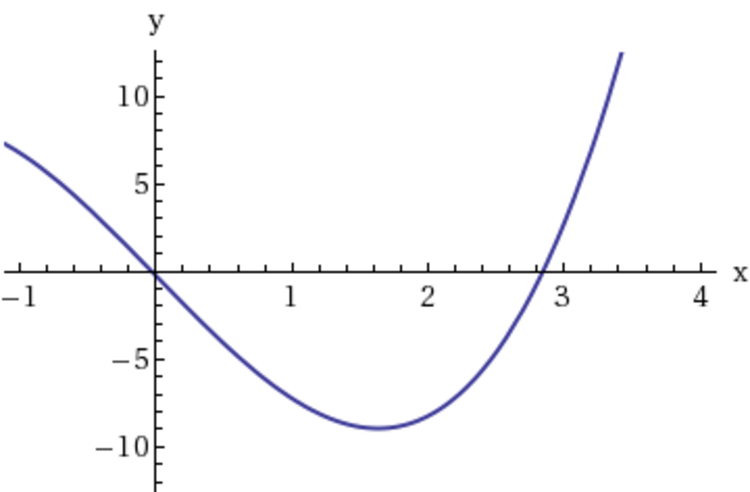
\includegraphics[width=3in]{./graphics/1711541.pdf} 
   \caption{WA-1711541}
   \label{fig:1711541}
\end{figure}
Which of the intervals of length $0.025$ contains this root?
\begin{parts}
\part $\left[2.825, \ 2.850\right]$

\begin{solution}
Work
\end{solution}

\part $\left[2.850, \ 2.875\right]$    

\begin{solution}
Work
\end{solution}
 
\part $\left[2.875, \ 2.900\right]$

\begin{solution}
Work
\end{solution}

\part $\left[2.900, \ 2.925\right]$

\begin{solution}
Work
\end{solution}


\part $\left[2.925, \ 2.950\right]$

\begin{solution}
Work
\end{solution}

\end{parts}
\end{questions}
\end{teacher}
\vfill
\pagebreak

%*-*-*-*-*-*-*-*-*-*-*-*-*-*-*-*-*-*-*-*-*-*-*-*-*-*-*-*-*-*-*-*-*-*-*-*-*-*-*-*-*-*-*-*-*-*-*-*-*-*-*-*-*-*-*-*-*-*-*-*-*-*-*-*-*-*-*-*-*-*-*-*-*-*-*-*-*-*-*-*-*-*-*-*-
\section{mth.121.03.01}
\subsection{The Derivative}


\subsubsection{Slope of Tangent Lines}
We will now return to the tangent line to the curve $y = f \left( x \right)$ at the point $\left( a, \ f \left( a \right)\right)$. As I hope you recall, this is where we started our initial discussion of calculus.



\textbf{Definition:} The \emph{tangent line} to the curve $y = f \left( x \right)$ at the point $\left( a, \ f \left( a \right)\right)$ is the line through  $\left( a, \ f \left( a \right)\right)$ with slope
\[
f'\left( a \right) = \mathop {\lim }\limits_{x \to a }  \frac{f \left( x \right) - f \left( a \right)}{x-a}
\]
provided the limit exists.



If $x \neq a$ you should note that
\[
\frac{f \left( x \right) - f \left( a \right)}{x-a}
\]
is just the slope of the secant line.



\textbf{Example:}  Find the equation of the line tangent to the curve
\[
y = \frac{2x}{\left(x+1\right)^2},
\]
at the point where $x=0$.\footnote{That means $a=0$.}


\begin{solution}
The point is $\left( 0, \ 0 \right)$ and the slope is
\begin{eqnarray*}
f'\left( 0 \right) &=& \lim_{x \to 0 }  \frac{f \left( x \right) - f \left( 0 \right)}{x-0}\\
&=& \lim_{x \to 0 }  \frac{2}{\left(x+1\right)^2}\\
&=& 2
\end{eqnarray*}
The equation is
\[
y - 0 = 2 \left( x - 0\right)
\]
\end{solution}

\subsubsection{Alternative Method}

Another way to write
\[
\mathop {\lim }\limits_{x \to a }  \frac{f \left( x \right) - f \left( a \right)}{x-a},
\]
is to use the letter $h$, as follows
\[
\mathop {\lim }\limits_{h \to 0 }  \frac{f \left( a+h \right) - f \left( a \right)}{h}.
\]
In fact, we have an exact equality:
\[
\mathop {\lim }\limits_{x \to a }  \frac{f \left( x \right) - f \left( a \right)}{x-a} = \mathop {\lim }\limits_{h \to 0 }  \frac{f \left( a+h \right) - f \left( a \right)}{h}.
\]



\textbf{Example:} Just for practice, try to find
\[
\mathop {\lim }\limits_{h \to 0 }  \frac{f \left( a+h \right) - f \left( a \right)}{h}.
\]
for
\[
y = \frac{2x}{\left(x+1\right)^2},
\]
at the point where $a=0$. It should agree with our prior result.

\begin{solution}
\begin{eqnarray*}
f'\left( 0 \right) &=& \lim_{h \to 0 }  \frac{f \left( 0+h \right) - f \left( 0 \right)}{h}\\
&=& \lim_{h \to 0 }  \frac{2}{\left( h + 1 \right)^2}\\
&=& 2 
\end{eqnarray*}
\end{solution}




\subsubsection{The Derivative at a Point}
\textbf{Definition:} The \emph{derivative at a point} where $x=a$ is denoted
\[
f'\left(a\right),
\]
and is found by evaluating the limit:
\[
\mathop {\lim }\limits_{h \to 0 }  \frac{f \left( a+h \right) - f \left( a \right)}{h},
\]
provided the limit exists.

This is often referred to as the instantaneous rate of change of $y =  f \left( x \right)$ with respect to $x$, when $x=a$ and is called the slope of the tangent line at $x=a$. Furthermore  the instantaneous rate of change of $s =  s \left( t \right)$ with respect to $t$, when $t=a$ is called the instantaneous velocity. Both concepts are the same, but depending on units, their interpretation can differ.


\subsubsection{The Derivative as a Function}


All the examples so far were at a given at a particular point, that is, some fixed value, but we can generalize this to any point where the limit is defined. The definition of the \emph{derivative as a function} simply follows from the above examples,
\[
f' \left( x \right) = \lim_{h \to 0 }  \frac{f \left( x+h \right) - f \left( x \right)}{h},
\]
provided the limit exists.\footnote{Now of course our new function will have a domain that may differ from the originating function. Yes, the derivative may not be defined at all points along the function.}


Finding derivatives, then using them, will take up much of this course. Right now we will be using the definition above to find this derived function, but in time we will be developing rules that will allows us to quickly find derivatives. Once these derivatives are found, we will then need to use them. They have many real applications, but that's for later.

 
\textbf{Example:} Find $f'\left(x\right)$ for
\[
f \left( x \right) = x^2 -3x +1.
\]
State the domain for both $f$ and $f'$.



\begin{solution}
The domain of $f$ is $\mathbb{R}$.
\begin{eqnarray*}
f' \left( x \right) &=& \lim_{h \to 0 }  \frac{f \left( x+h \right) - f \left( x \right)}{h}\\
&=&  \lim_{h \to 0 }  \frac{ \left( x+h \right)^2 - 3\left( x+h \right) + 1 - \left( x^2 -3x +1 \right) }{h}\\
&=&  \lim_{h \to 0 }  \frac{2xh + h^2 -3h }{h}\\
&=&  \lim_{h \to 0 }  2x + h - 3\\
&=& 2x-3
\end{eqnarray*}
The domain of $f'$ is also $\mathbb{R}$.
\end{solution}


 
 
\subsection{Examples}
\begin{questions}


\question Find $f'\left(a\right)$.
\[
f\left(x\right) = x^{-2}, \quad a = 3
\]

\begin{solution}
We'll discuss this in class.

\begin{eqnarray*}
f'\left( 3 \right) &=& \lim_{x \to 3 }  \frac{f \left( x \right) - f \left( 3 \right)}{x-3}\\
&=& \lim_{x \to 3 }  \frac{1/x^2 - 1/9}{x-3} \cdot \frac{9x^2}{9x^2}\\
&=& \lim_{x \to 3 } \frac{9-x^2}{9x^2\left(x-3\right)}\\
&=& \lim_{x \to 3 } -\frac{3+x}{9x^2}\\
&=& -\frac{2}{27}
\end{eqnarray*}
\end{solution}



\question Find $f'\left(a\right)$ at $a=1$, for
\[
f \left( x \right) = \sqrt{x+1}.
\]

\begin{solution}
We'll discuss this in class.

\begin{eqnarray*}
f'\left( 1 \right) &=& \lim_{x \to 1 }  \frac{f \left( x \right) - f \left( 1 \right)}{x-1}\\
&=&  \lim_{x \to 1 }  \frac{ \sqrt{x+1}  - \sqrt{2} }{x-1} \cdot \frac{\sqrt{x+1} + \sqrt{2}}{\sqrt{x+1} + \sqrt{2}} \\
&=&  \lim_{x \to 1 }   \frac{1}{\sqrt{x+1} + \sqrt{2}} \\
&=& \frac{1}{2\sqrt{2}}
\end{eqnarray*}

\end{solution}



\question Find $f'\left(a\right)$.
\[
f\left(x\right) = \frac{1}{\sqrt{2x+1}}, \quad a = 4
\]

\begin{solution}
We'll discuss this in class.

\begin{eqnarray*}
f'\left( 4 \right) &=& \lim_{x \to 4 }  \frac{f \left( x \right) - f \left( 4 \right)}{x-4}\\
&=& \ldots \quad \mbox{Work will be done in class.}\\
&=& -\frac{1}{27}
\end{eqnarray*}
\end{solution}

\question Given the following graph (Figure \ref{fig:graph0901}, page \pageref{fig:graph0901}) estimate $f'\left(-2\right)$ and then estimate the equation of the tangent line at the point $\left( -2, \ f'\left(-2\right)\right)$.
\begin{figure}[htbp] %  figure placement: here, top, bottom, or page
   \centering
   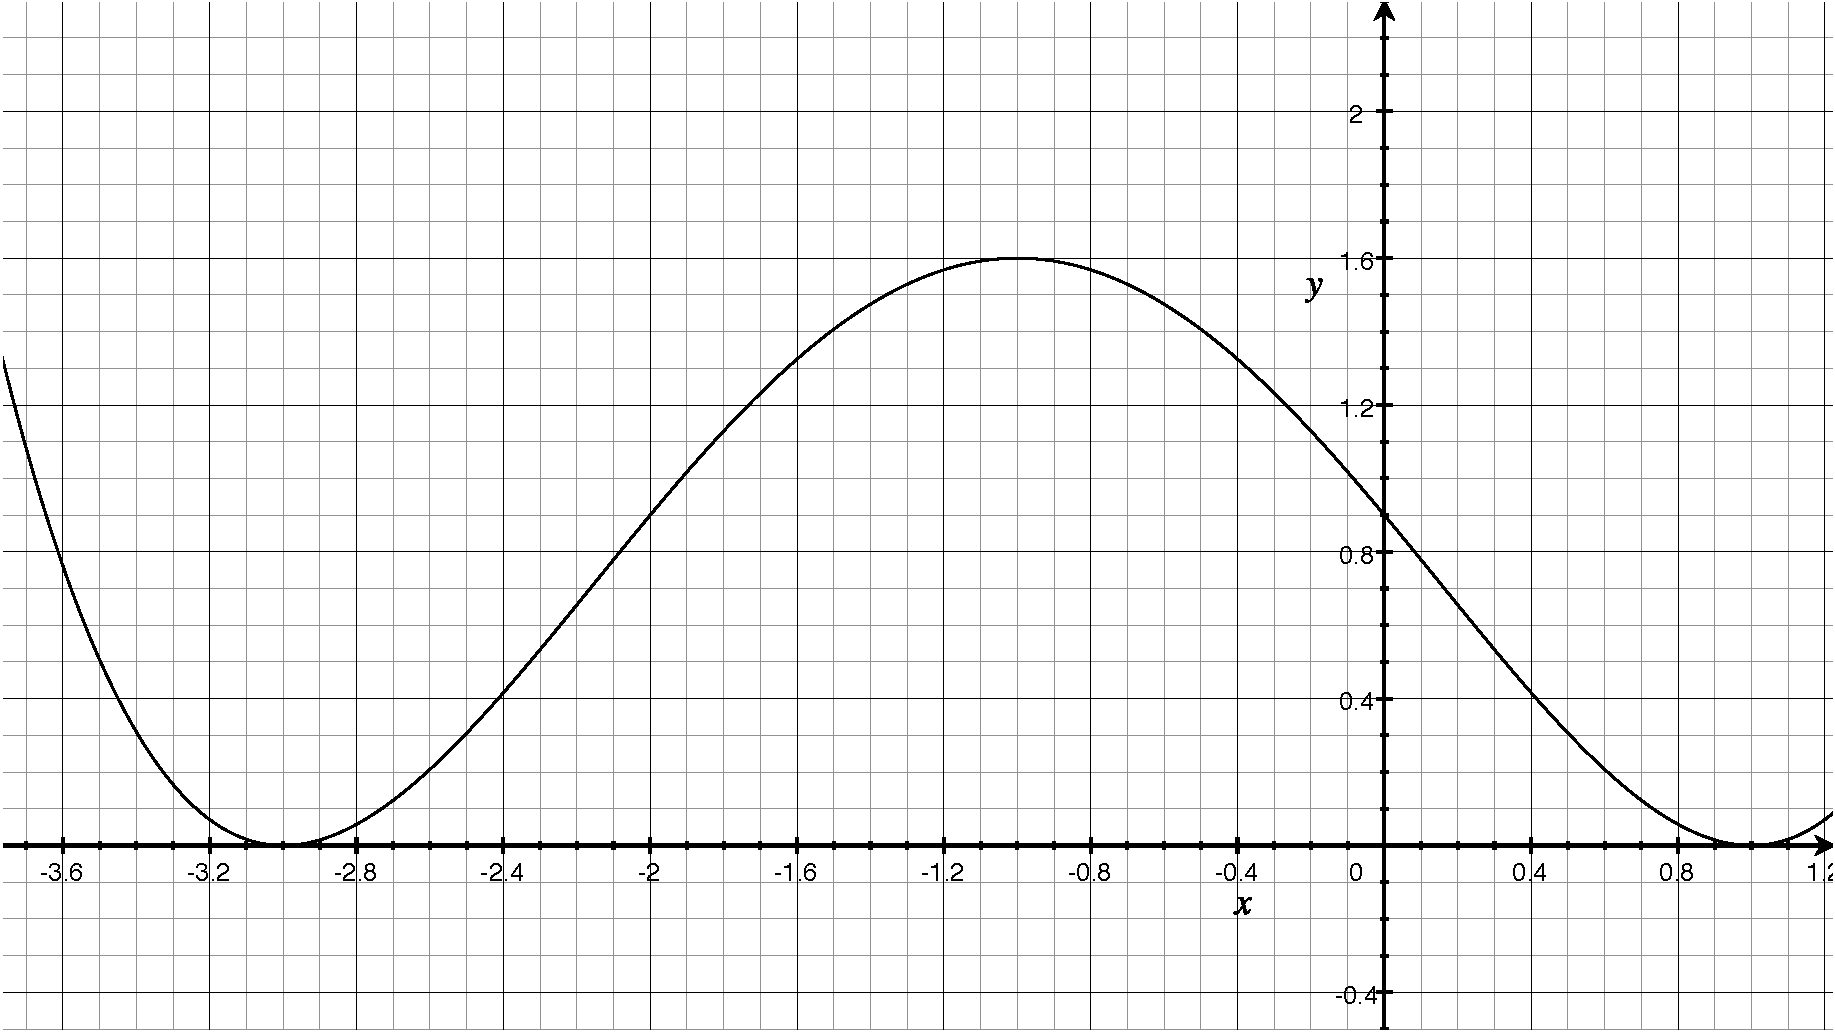
\includegraphics[width=5in]{./graphics/graph0901.pdf} 
   \caption{A partial graph of $f$.}
   \label{fig:graph0901}
\end{figure}

\begin{solution}
We'll discuss this in class.

By inspection the point is approximately $\left( -2, \ 0.9 \right)$ and the slope of the line tangent to the curve at this point is approximately $m =f'\left(-2\right)= 1.3$. So the equation of the tangent line is
\[
y - 0.9 = 1.3 \left( x + 2\right).
\]
\end{solution}

\question Find $f'\left(x\right)$ for
\[
f \left( x \right) = \frac{1 + x}{1 - x}.
\]
State the domain for both $f$ and $f'$.

\begin{solution}
We'll discuss this in class.

The domain of $f$ is $\mathbb{R}, \ x \neq 1$.
\begin{eqnarray*}
f' \left( x \right) &=& \lim_{h \to 0 }  \frac{f \left( x+h \right) - f \left( x \right)}{h}\\
&=& \ldots \quad \mbox{Work will be done in class.}\\
&=&\frac{2}{\left( 1-x\right)^2}
\end{eqnarray*}
The domain of $f'$ is also $\mathbb{R}, \ x \neq 1$.
\end{solution}



\question Find $f'\left(x\right)$ for
\[
f \left( x \right) = \sqrt{1-x}.
\]
State the domain for both $f$ and $f'$.

\begin{solution}
We'll discuss this in class.

The domain of $f$ is $\left( -\infty, \ 1 \right]$.
\begin{eqnarray*}
f' \left( x \right) &=& \lim_{h \to 0 }  \frac{f \left( x+h \right) - f \left( x \right)}{h}\\
&=& \ldots \quad \mbox{Work will be done in class.}\\
&=&- \frac{1}{2\sqrt{1-x}}
\end{eqnarray*}
The domain of $f'$ is $\left( -\infty, \ 1 \right)$. They do differ!
\end{solution}



\end{questions}







%
%
%\section{Examples}
%
%\begin{enumerate}
%
%\item The position (miles) of a particle after $t$ minutes moving along a straight line is given by
%\[
%s\left( t \right) = \frac{t^2}{2} - \frac{t^3}{12}, \qquad 0 \leq t \leq 4.
%\]
%\begin{enumerate}
%\item Approximate the velocity at $t=2$ in miles per hour (mph). Here, you should use
%\[
%\frac{\Delta s}{\Delta t} = \frac{s\left(t\right) - s\left(2\right)}{t-2},
%\]
%and select a series of small time intervals to find a possible pattern.
%
%\vfill
%\pagebreak
%
%\item Use the definition of instantaneous velocity (mph) to computer the instantaneous velocity at $t=2$. Using one of these limits:
%\[
%v\left(2\right)= \mathop {\lim }\limits_{t \to 2 } \frac{s\left(t\right) - s\left(2\right)}{t-2} =
%\mathop {\lim }\limits_{h \to 0 } \frac{s\left(2 + h\right) - s\left(2\right)}{h}.
%\]
%
%\vspace{2in}
%
%\end{enumerate}
%
%\vspace{1.5in}
%
%\item The position function, $f \left( t \right)$ in meters and $t$ in seconds, is given by
%\[
%f \left( t \right) = -16t^2 + 5.
%\]
%Find $f' \left( a \right)$ and then interpret $f' \left( 3 \right)$.
% 
%\vfill
%\pagebreak
%
%
%\item Given
%\[
%f \left( x \right) = \frac{1}{\sqrt{x-1}},
%\]
%find $f' \left( x \right)$ using\footnote{The pre-requisites for success in calculus is certainly knowing algebra and being able to deal with a variety of functions.}
%\[
%f' \left( x \right) = \mathop {\lim }\limits_{h \to 0 }  \frac{f \left( x+h \right) - f \left( x \right)}{h}.
%\]
%
%\end{enumerate}











\subsection{Assignment}
You should read \S  3.1 and do the WebAssign assignment mth.121.03.01.
\vfill
\pagebreak
%*-*-*-*-*-*-*-*-*-*-*-*-*-*-*-*-*-*-*-*-*-*-*-*-*-*-*-*-*-*-*-*-*-*-*-*-*-*-*-*-*-*-*-*-*-*-*-*-*-*-*-*-*-*-*-*-*-*-*-*-*-*-*-*-*-*-*-*-*-*-*-*-*-*-*-*-*-*-*-*-*-*-*-*-

\begin{teacher}
\subsection{Assessments}
The following questions are related to the WebAssign assignments and may be used to assess students' ability. Please do not share any of these questions with students.
\begin{questions}		
\question 	%RogaCalcET2 3.1.001	WA-1731819


Let $f\left(x\right) = 3x^2$.
\begin{parts}
\part Find $f\left(3 + h\right)$.
\part Find $\displaystyle \frac{f\left(3 + h\right) - f\left(3\right)}{4}$.
\part Compute $f'\left(3\right)$ by taking the limit as $h \to 0$.
\end{parts}

\question 	%RogaCalcET2 3.1.005	WA-1761626

Compute $f'\left(a\right)$ in two ways.
\[
f\left(x\right) = 7 + 5x + 2x^2, \quad a = 5
\]
\begin{parts}
\part $\displaystyle f'\left( a \right) = \lim_{h \to 0} \frac{f\left(a+h\right) - f\left(a\right)}{h}$.
\part $\displaystyle f'\left( a \right) = \lim_{x \to a} \frac{f\left(x\right) - f\left(a\right)}{x-a}$.
\end{parts}

\question 	%RogaCalcET2 3.1.007	WA-1731854

Problem 7 \S3.1.

\question 	%RogaCalcET2 3.1.009	WA-1731850

Problem 9 \S3.1.

\question 	%RogaCalcET2 3.1.011	WA-1761129

Problem 11 \S3.1.

\question 	%RogaCalcET2 3.1.012	WA-1731899

Problem 12 \S3.1.

\question 	%RogaCalcET2 3.1.014	WA-1714524

Problem 14 \S3.1.

\question 	%RogaCalcET2 3.1.015	WA-1731890

Use the limit definition to calculate the derivative of the linear function.
\[
f\left(x\right) = 9x - 5
\]

\question 	%RogaCalcET2 3.1.019	WA-1632547

What is an equation of the tangent line at $x = 3$, assuming that $y\left(3\right) = 5$ and $y'\left(3\right) = 2$.




\question 	%RogaCalcET2 3.1.020	WA-1731848


Find $f\left( 3 \right)$ and $f'\left(3\right)$, assuming that the tangent line to $y = f\left(x\right)$ at $a = 3$ has equation $y = 3x + 7$.

\question 	%RogaCalcET2 3.1.022	WA-1739492


Suppose that $f\left (x\right)$ is a function such that the relationship given below is true.
\[
f \left(5 + h\right) - f \left(5\right) = 6h^2 + 3h 
\]
\begin{parts}
\part What is $f '\left(5\right)$?
\begin{solution}
3
\end{solution}
\part What is the slope of the secant line through $\left(5, \ f \left(5\right)\right)$ and $\left(8, \ f \left(8\right)\right)$?
\begin{solution}
21
\end{solution}
\end{parts}


\question 	%RogaCalcET2 3.1.025	WA-1731912

Let $f\left(x\right) = \displaystyle \frac{1}{\sqrt{7x}}$. Compute
\[
\lim_{h \to 0} \frac{f\left(5 + h\right) - f\left(5\right)}{h} 
\]


\question 	%RogaCalcET2 3.1.028	WA-1731897

Use the limit definition to compute $f'\left(a\right)$.
\[
f\left(x\right) = 11 - x^2, \quad a = -1
\]
Find an equation of the tangent line. (Enter your answer as an equation using the variables $y$ and $x$.)


\question 	%RogaCalcET2 3.1.035	WA-1714520

Use the limit definition to compute the derivative of the function at $x = -7$.
\[
f\left(x\right) = \frac{1}{x+9}
\]
And find an equation of the tangent line at $x = -7$.

\question 	%RogaCalcET2 3.1.052	WA-1714541

The limit represents a derivative $f'\left(a\right)$. Find $f\left(x\right)$ and $a$.
\[
\lim_{x \to 2} \frac{x^4-16}{x-2}
\]

\question 	%RogaCalcET2 3.1.061	WA-1714555

Problem 61 \S3.1

\end{questions}
\end{teacher}

\vfill
\pagebreak

%*-*-*-*-*-*-*-*-*-*-*-*-*-*-*-*-*-*-*-*-*-*-*-*-*-*-*-*-*-*-*-*-*-*-*-*-*-*-*-*-*-*-*-*-*-*-*-*-*-*-*-*-*-*-*-*-*-*-*-*-*-*-*-*-*-*-*-*-*-*-*-*-*-*-*-*-*-*-*-*-*-*-*-*-
\section{mth.121.03.02}
\subsection{Finding Derivatives}


The definition of the \emph{derivative as a function} is,
\[
f' \left( x \right) = \mathop {\lim }\limits_{h \to 0 }  \frac{f \left( x+h \right) - f \left( x \right)}{h},
\]
provided the limit exists.\footnote{Now of course our new function will have a domain that may differ from the originating function. Yes, the derivative may not be defined at all points along the function.}



From here on out the following \emph{new} notation will also be used.
\[
f' \left( x \right) = \frac{{\rm{d}}}{{\rm{d}}x} \ \left[ f \left( x \right) \right] = \mathop {\lim }\limits_{h \to 0 }  \frac{f \left( x+h \right) - f \left( x \right)}{h}
\]


This is the definition that you are supposed to use if you are asked to find the derivative of a function by using the definition. However, we can also use this definition to develop simple rules for a colossal number of functions. That's good news, because if you were asked to find the derivative of
\[
f \left( x \right) = \sqrt{ \frac{ \left(x^3-3x^2+5x-9\right)^{200} - 1 }{ \sin x^2 - \cos^2 x } } 
\]
by definition, you would probably get stuck very quickly. In time you will be able to find the derivative of this particular function very quickly.


 
First, I will present some rules, then we will apply them to problems.
Some rules will be proved, and you should be able to follow what's being presented in class.



\subsubsection{Constants}
Suppose $f\left( x \right) = k$, where $k$ is any constant.
\begin{eqnarray*}
f' \left( x \right) &=& \mathop {\lim }\limits_{h \to 0 }  \frac{f \left( x+h \right) - f \left( x \right)}{h}\\
&=& \mathop {\lim }\limits_{h \to 0 }  \frac{k - k}{h}\\
&=& \mathop {\lim }\limits_{h \to 0 }  \frac{0}{h} = 0
\end{eqnarray*}
Notational we will write this rule as follows. If $f\left(x\right) = k$, where $k$ is any constant, then
\[
f' \left( x \right) = \frac{{\rm{d}}}{{\rm{d}}x} \ \left[ k \right]= \frac{{\rm{d}}}{{\rm{d}}x} \ \left[ f \left( x \right) \right]= 0.
\]



\subsubsection{Power Rule}
Suppose $f\left( x \right) = x^n$, where $n$ is any positive integer.\footnote{The Binomial Theorem and its application to this problem will be discussed in class.}
\begin{eqnarray*}
f' \left( x \right) &=& \mathop {\lim }\limits_{h \to 0 }  \frac{f \left( x+h \right) - f \left( x \right)}{h}\\
&=& \mathop {\lim }\limits_{h \to 0 }  \frac{ \left( x+h \right)^n - x^n}{h}\\
&=& \mathop {\lim }\limits_{h \to 0 }  \frac{x^n + nx^{n-1}h + \cdots + h^n - x^n}{h}\\
&=& \mathop {\lim }\limits_{h \to 0 }  nx^{n-1} + \mbox{ terms with a factor of $h$}\\
&=& nx^{n-1}
\end{eqnarray*}
Notational we will write this rule as follows. If $f\left(x\right) = x^n$, where $n$ is any positive integer, then
\[
f' \left( x \right) = \frac{{\rm{d}}}{{\rm{d}}x} \ \left[ x^n \right]= \frac{{\rm{d}}}{{\rm{d}}x} \ \left[ f \left( x \right) \right]= nx^{n-1}.
\]

\subsubsection{Other Simple Rules}
Suppose $f\left( x \right)$ and  $g\left( x \right)$ are differentiable at $x$ and $c$ is any constant, then\footnote{This will be discussed in class.}
\begin{enumerate}
\item The derivative of a sum is the sum of the derivatives.
\[
\frac{{\rm{d}}}{{\rm{d}}x} \ \left[ f\left( x \right) +  g\left( x \right) \right]  = f'\left( x \right) +  g'\left( x \right)
\]
\item The derivative of a difference is the difference of the derivatives.
\[
\frac{{\rm{d}}}{{\rm{d}}x} \ \left[ f\left( x \right) -  g\left( x \right) \right]  = f'\left( x \right) -  g'\left( x \right)
\]
\item The derivative of a constant multiple of a function is the constant times the derivative of the function.
\[
\frac{{\rm{d}}}{{\rm{d}}x} \ \left[ c \cdot f\left( x \right) \right]  = c \cdot f'\left( x \right)
\]
\item \textbf{Product Rule:} The derivative of the product of two functions is the first function times the derivative of the second function plus the second function times the derivative of the first function.\footnote{The product rule is being mentioned here, but will not be used until later.}
\[
\frac{{\rm{d}}}{{\rm{d}}x} \ \left[ f\left( x \right) \cdot g\left( x \right) \right]  = f\left( x \right) \cdot g'\left( x \right) + g\left( x \right) \cdot f'\left( x \right)
\]
\item \textbf{Quotient Rule:} The derivative of a quotient is the denominator times the derivative of the numerator minus the numerator times the derivative of the denominator; all divided by the square of the denominator.\footnote{The quotiet rule is being mentioned here, but will not be used until later.}
\[
\frac{{\rm{d}}}{{\rm{d}}x} \ \left[ \frac{f\left( x \right)}{g\left( x \right)} \right]  = \frac{g\left( x \right) \cdot f'\left( x \right) - f\left( x \right) \cdot g'\left( x \right)}{\left[ g\left( x \right)\right]^2} \]
\end{enumerate}
\subsubsection{Exponential Functions}

Material covered in MTH-119 is extremely important and exponential functions are no exception. Recall that the general exponential function is of the form,
\[
f\left( x\right) = a^x,
\]
where $a$ is a positive constant, and $a \neq 1$. You should, of course, review the material that you learned in MTH-119. Specifically you should be able to solve exponential equations, and also graph simple exponential functions.

\subsubsection{Derivatives of Exponential Functions}

Recall that the derivative of a function is found by evaluating a limit. For example, if $f\left( x\right) = a^x$, then
\begin{eqnarray*}
f'\left( x \right) = \mathop {\lim }\limits_{h\to 0} \frac{f \left( x + h \right) - f \left( x \right)}{h} &=& \mathop {\lim }\limits_{h\to 0} \frac{a^{x+h} - a^x}{h}\\
&=& a^x \mathop {\lim }\limits_{h\to 0} \frac{a^{h} - 1}{h}.
\end{eqnarray*}
The tough part is evaluating the limit, but first observe that
\[
f'\left( 0 \right) = \mathop {\lim }\limits_{h\to 0} \frac{a^h - 1}{h},
\]
so
\[
f'\left( x \right) = a^x f'\left( 0 \right).
\]



\textbf{Definition:} Euler's number is indicated by $e$, where
\[
\mathop {\lim }\limits_{h\to 0} \frac{e^h - 1}{h} = 1.
\]

This, of course leads to the following important result.
\[
\frac{{\rm{d}}}{{\rm{d}}x} \left( e^x \right) = e^x
\]











\subsubsection{Generalized Power Rule}
If $f\left( x \right) = x^r$, where $r \in \mathbb{R}$, then
\[
f' \left( x \right) = \frac{{\rm{d}}}{{\rm{d}}x} \ \left[ x^r \right] = rx^{r-1}.
\]
As you may recall from MTH-120 you were presented with the Binomial Theorem for positive integers only, so the proof of this power rule is not so simple. Actually the proof involves using logarithms, and we will have to wait until we do logarithmic differentiation.











\subsection{Examples}
Show all work and box the final answer.
\begin{questions}
\question Compute $f'\left(x\right)$ using the limit definition and rules.
$ \displaystyle f \left( x \right) = e^\pi$

\begin{solution}
We'll discuss this in class.

$e^\pi$ is a \emph{constant}!
\[
f'\left( x \right) = 0
\]
\end{solution}

\question Differentiate the function.
$ \displaystyle f \left( x \right) = \frac{5x^8}{4}$

\begin{solution}
We'll discuss this in class.

\[
f'\left( x \right) = 10x^7
\]
\end{solution}

\question Compute $f'\left(x\right)$ using the limit definition and rules.
$ \displaystyle f \left( x \right) = 5x^2 - 3x + 1$

\begin{solution}
We'll discuss this in class.

\[
f'\left( x \right) = 10x-3
\]
\end{solution}


\question Differentiate the function.\footnote{Do not use the product rule.}
$ \displaystyle f \left( x \right) = \left( x - 2 \right) \cdot \left( 2x - 5 \right)$

\begin{solution}
We'll discuss this in class.

You'll need to expand before differentiating.
\begin{eqnarray*}
 f \left( x \right) &=& \left( x - 2 \right) \cdot \left( 2x - 5 \right)\\
 &=& 2x^2-9x+10\\
 f'\left(x\right) &=& 4x-9
\end{eqnarray*}

\end{solution}


\question Compute $f'\left(x\right)$ using the limit definition and rules.
$ \displaystyle f \left( x \right) = \sqrt{x}$

\begin{solution}
We'll discuss this in class.

By \emph{definition}.
\begin{eqnarray*}
f' \left( x \right) &=& \lim_{h \to 0 }  \frac{f \left( x+h \right) - f \left( x \right)}{h}\\
&=& \lim_{h \to 0 }  \frac{ \sqrt{x+h} -  \sqrt{x}}{h} \cdot \frac{\sqrt{x+h} +  \sqrt{x}}{\sqrt{x+h} +  \sqrt{x}}\\
&=& \lim_{h \to 0 }  \frac{h}{h \cdot \left( \sqrt{x+h} +  \sqrt{x} \right)} \\
&=& \frac{1}{2\sqrt{x}}
\end{eqnarray*}

By \emph{rule}.
\begin{eqnarray*}
 f \left( x \right) &=& \sqrt{x}\\
 &=& x^{1/2}\\
 f'\left( x \right) &=& \frac{1}{2}x^{-1/2}
\end{eqnarray*}

Make sure you understand the difference between \emph{rule} and \emph{definition}. You should also note that the above two answers are identical.
\[
 f'\left( x \right) = \frac{1}{2}x^{-1/2} =  \frac{1}{2\sqrt{x}} =  \frac{\sqrt{x}}{2x}
\]
\end{solution}


\question Differentiate the function.\footnote{Do not use the product rule.}
$ \displaystyle f \left( x \right) = \left( x^2 - 2x + 3\right)^2$

\begin{solution}
We'll discuss this in class.

You'll need to expand and then differentiate.
\begin{eqnarray*}
 f \left( x \right) &=& \left( x^2 - 2x + 3\right)^2\\
 &=& x^4 -4x^3+10x^2-12x+9\\
  f' \left( x \right) &=& 4x^3 -12x^2+20x-12
\end{eqnarray*}

\end{solution}


\question Differentiate the function.\footnote{Do not use the quotient rule.}
$ \displaystyle f \left( x \right) = \frac{x^2-1}{x+1}$

\begin{solution}
We'll discuss this in class.

Simplify first!
\begin{eqnarray*}
 f \left( x \right) &=& \frac{x^2-1}{x+1}\\
 &=& x-1\\
  f' \left( x \right) &=& 1, \quad x \neq 1
\end{eqnarray*}

\end{solution}


\question Differentiate the function.
$ \displaystyle f \left( x \right) = 3\sqrt{x} - \frac{5}{\sqrt[3]{x}}$

\begin{solution}
We'll discuss this in class.

\begin{eqnarray*}
f \left( x \right) &=&  3\sqrt{x} - \frac{5}{\sqrt[3]{x}}\\
 &=& 3x^{1/2} - 5x^{-1/3}\\
f' \left( x \right) &=& \frac{3}{2}x^{-1/2} + \frac{5}{3}x^{-4/3}
\end{eqnarray*}
\end{solution}

\question Differentiate the function.
$ \displaystyle f \left( x \right) = x \sqrt{x}$

\begin{solution}
We'll discuss this in class.

\[
f '\left( x \right) = \frac{3}{2} x^{1/2}
\]
\end{solution}


\question Differentiate the function.
$ \displaystyle f \left( x \right) = \left( 3\sqrt{x} - \frac{5}{\sqrt[3]{x}} \right)^2$

\begin{solution}
We'll discuss this in class.

Expand and then differentiate.
\begin{eqnarray*}
f \left( x \right) &=& \left( 3\sqrt{x} - \frac{5}{\sqrt[3]{x}} \right)^2\\
 &=& 9x -30x^{1/6} + 25x^{-2/3}\\
f' \left( x \right) &=& 9 - 5 x^{-5/6} - \frac{50}{3}x^{-5/3}
\end{eqnarray*}

\end{solution}




\question Differentiate the function.\footnote{This is a function of $x$, that is, the variable is $x$ and $A$, $B$ and $C$ are constants.}
$ \displaystyle f \left( x \right) = Ax^2 + Bx + C$

\begin{solution}
We'll discuss this in class.

\[
f'\left( x \right) = 2Ax+B
\]
\end{solution}





\question Differentiate the function.
$ \displaystyle f \left( x \right) = e^{x+1}$

\begin{solution}
We'll discuss this in class.

\[
 f' \left( x \right) = e^{x+1}
\]
\end{solution}

\question Find the equation of the tangent line to the curve $ \displaystyle f \left( x \right) = \left( e^x - 1 \right)^2$, given that
\[
f' \left( x \right) = 2 e^x \left( e^x - 1 \right),
\] at the point $x=0$. A graph (Figure \ref{fig:graph1005}, page \pageref{fig:graph1005}) is provided, please indicate both $f$ and the line tangent to $f$ at $x=0$.
\begin{figure}[htbp] %  figure placement: here, top, bottom, or page
   \centering
   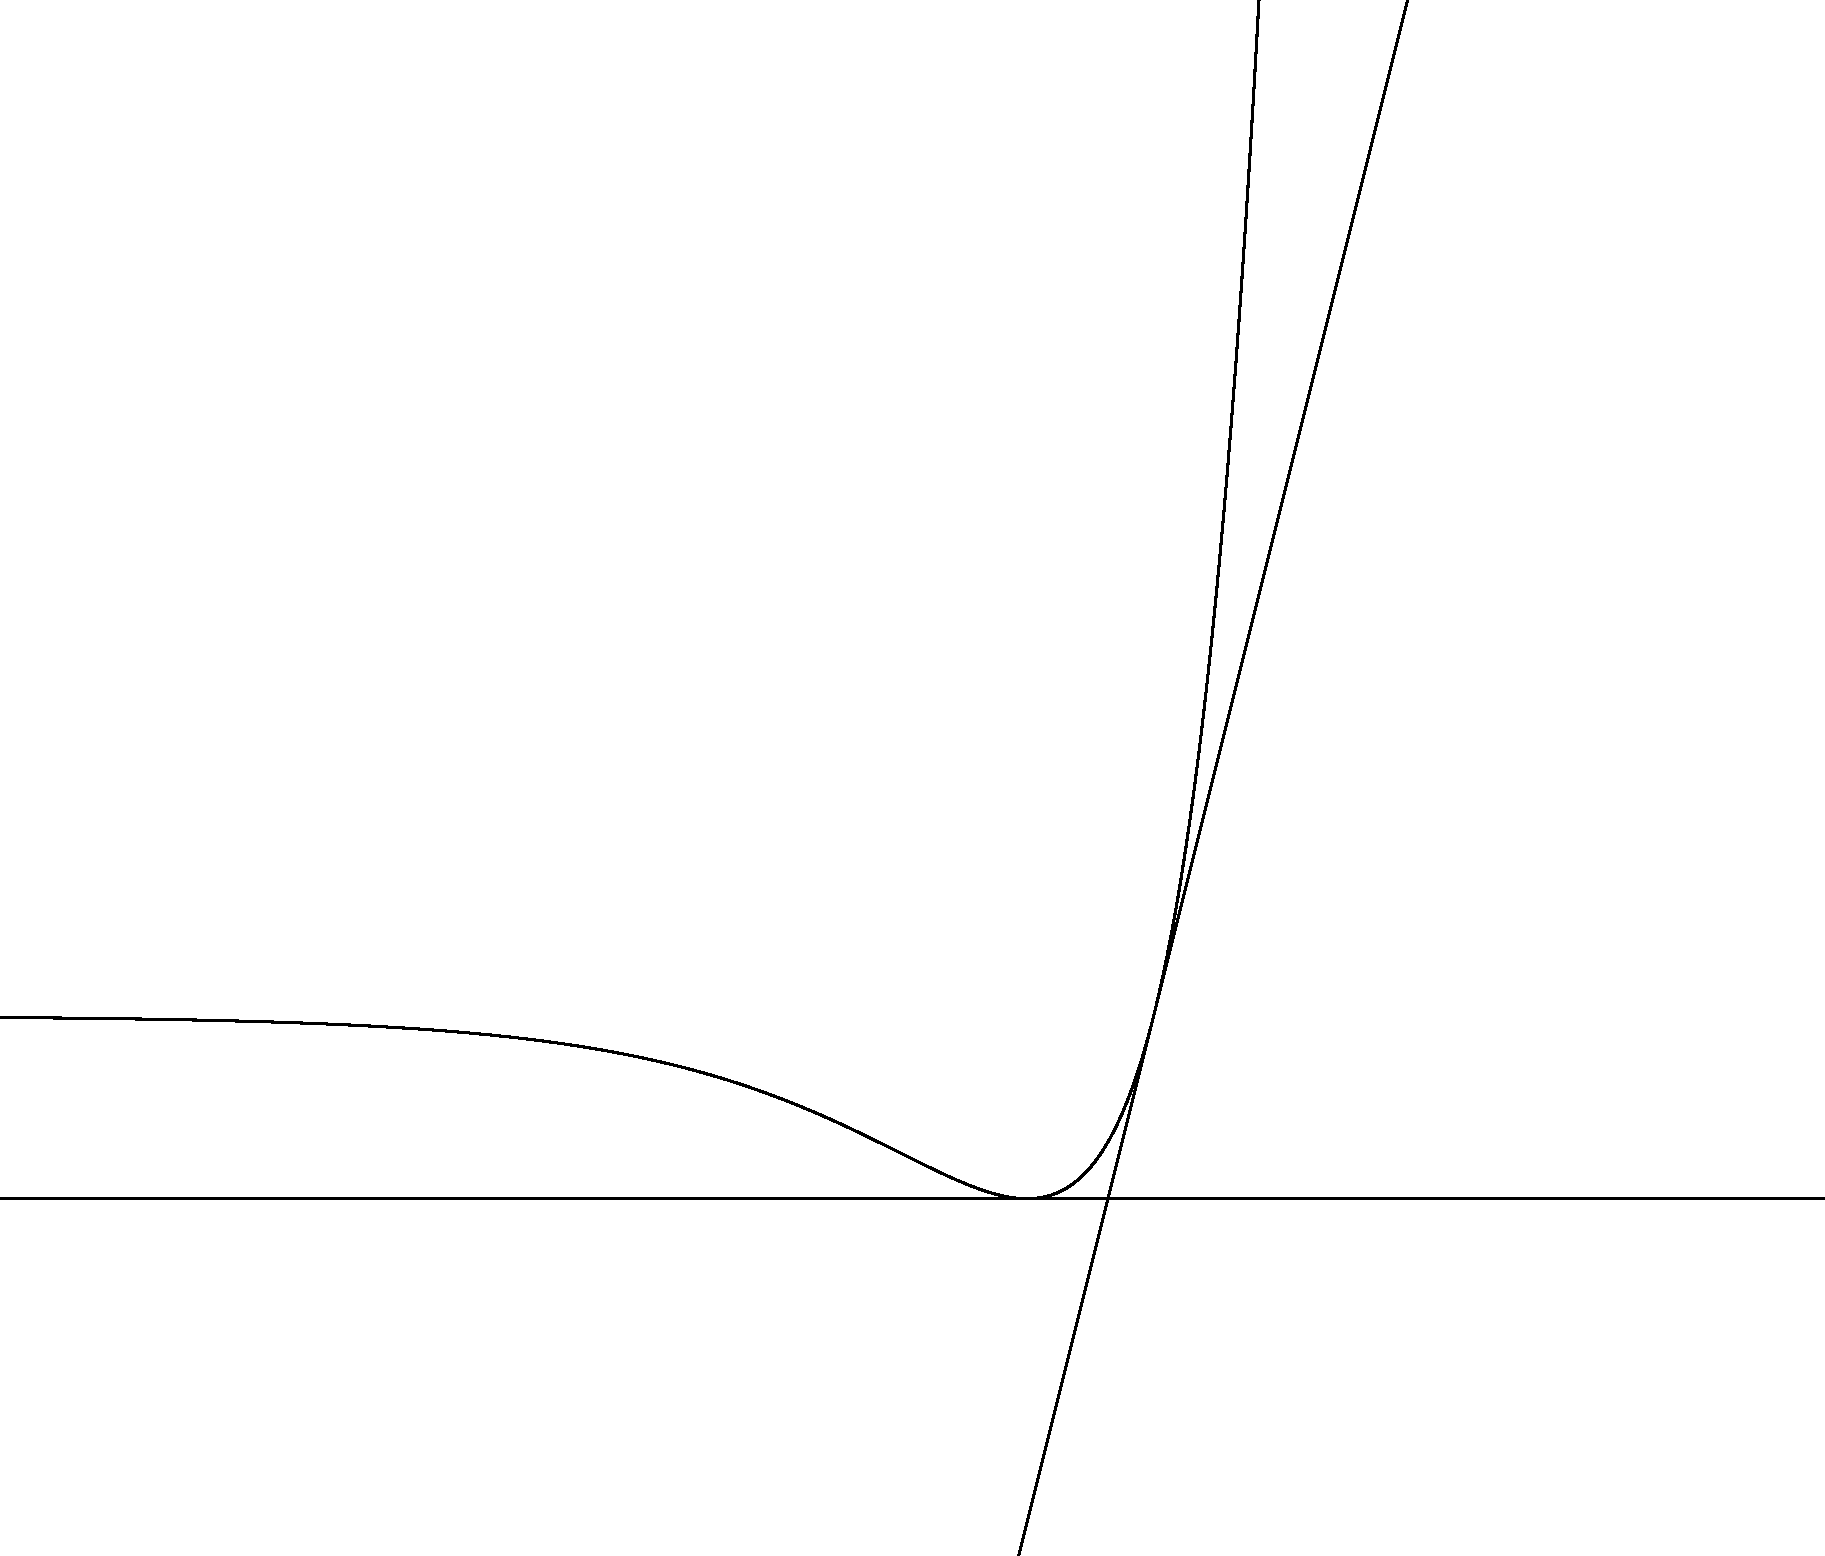
\includegraphics[width=4in]{./graphics/graph1005.pdf} 
   \caption{Partial graph of $f$ and two tangent lines to $f$ at $x=0$ and $x=\ln 2$.}
   \label{fig:graph1005}
\end{figure}

\begin{solution}
This will be discussed in class.

This is the horizontal line, point of tangency is $\left( 0, \ 0 \right)$, and slope of the tangent is $m=0$.
\[
y = 0
\]
\end{solution}

\question Find the equation of the tangent line to the curve $ \displaystyle f \left( x \right) = \left( e^x - 1 \right)^2$ at the point $x=\ln 2$. A graph (Figure \ref{fig:graph1005}, page \pageref{fig:graph1005}) is provided, please indicate both $f$ and the line tangent to $f$ at $x= \ln 2$.


\begin{solution}
We'll discuss this in class.

This is the non-horizontal line, point of tangency is $\left( \ln 2, \ 1 \right)$, and slope of the tangent is $m=4$.
\[
y -1 = 4 \left( x - \ln 2 \right)
\]
\end{solution}



\end{questions}





\subsection{Assignment}
You should read \S  3.2 and do the WebAssign assignment mth.121.03.02.
\vfill
\pagebreak
%*-*-*-*-*-*-*-*-*-*-*-*-*-*-*-*-*-*-*-*-*-*-*-*-*-*-*-*-*-*-*-*-*-*-*-*-*-*-*-*-*-*-*-*-*-*-*-*-*-*-*-*-*-*-*-*-*-*-*-*-*-*-*-*-*-*-*-*-*-*-*-*-*-*-*-*-*-*-*-*-*-*-*-*-
\begin{teacher}
\subsection{Assessments}
The following questions are related to the WebAssign assignments and may be used to assess students' ability. Please do not share any of these questions with students.
\begin{questions}		
\question 	%RogaCalcET2 3.2.001	WA-1731830

Compute $f'\left(x\right)$ using the limit definition.
\[
f\left(x\right) = 3x - 7
\]
\begin{solution}
Work.
\end{solution}

\question 	%RogaCalcET2 3.2.002	WA-1731920

Compute $f'\left(x\right)$ using the limit definition.
\[
f\left(x\right) = x^2+13x
\]
\begin{solution}
Work.
\end{solution}

\question 	%RogaCalcET2 3.2.004	WA-1731870

Compute $f'\left(x\right)$ using the limit definition.
\[
f\left(x\right) = 1 - 3x^{-1}
\]
\begin{solution}
Work.
\end{solution}

\question 	%RogaCalcET2 3.2.005	WA-1731858

Compute $f'\left(x\right)$ using the limit definition.
\[
f\left(x\right) = 13x - \sqrt{x}
\]
\begin{solution}
Work.
\end{solution}

\question 	%RogaCalcET2 3.2.006	WA-1716668

Compute $f'\left(x\right)$ using the limit definition.
\[
f\left(x\right) = \left( 2x \right)^{-1/2} + 3
\]
\begin{solution}
Work.
\end{solution}

\question 	%RogaCalcET2 3.2.043	WA-1760268

Problem 43 \S3.2
\begin{solution}
Work.
\end{solution}


\question 	%RogaCalcET2 3.2.044	WA-1722185


Of the two functions in figure below which is the derivative of the other?
\begin{figure}[htbp] %  figure placement: here, top, bottom, or page
   \centering
   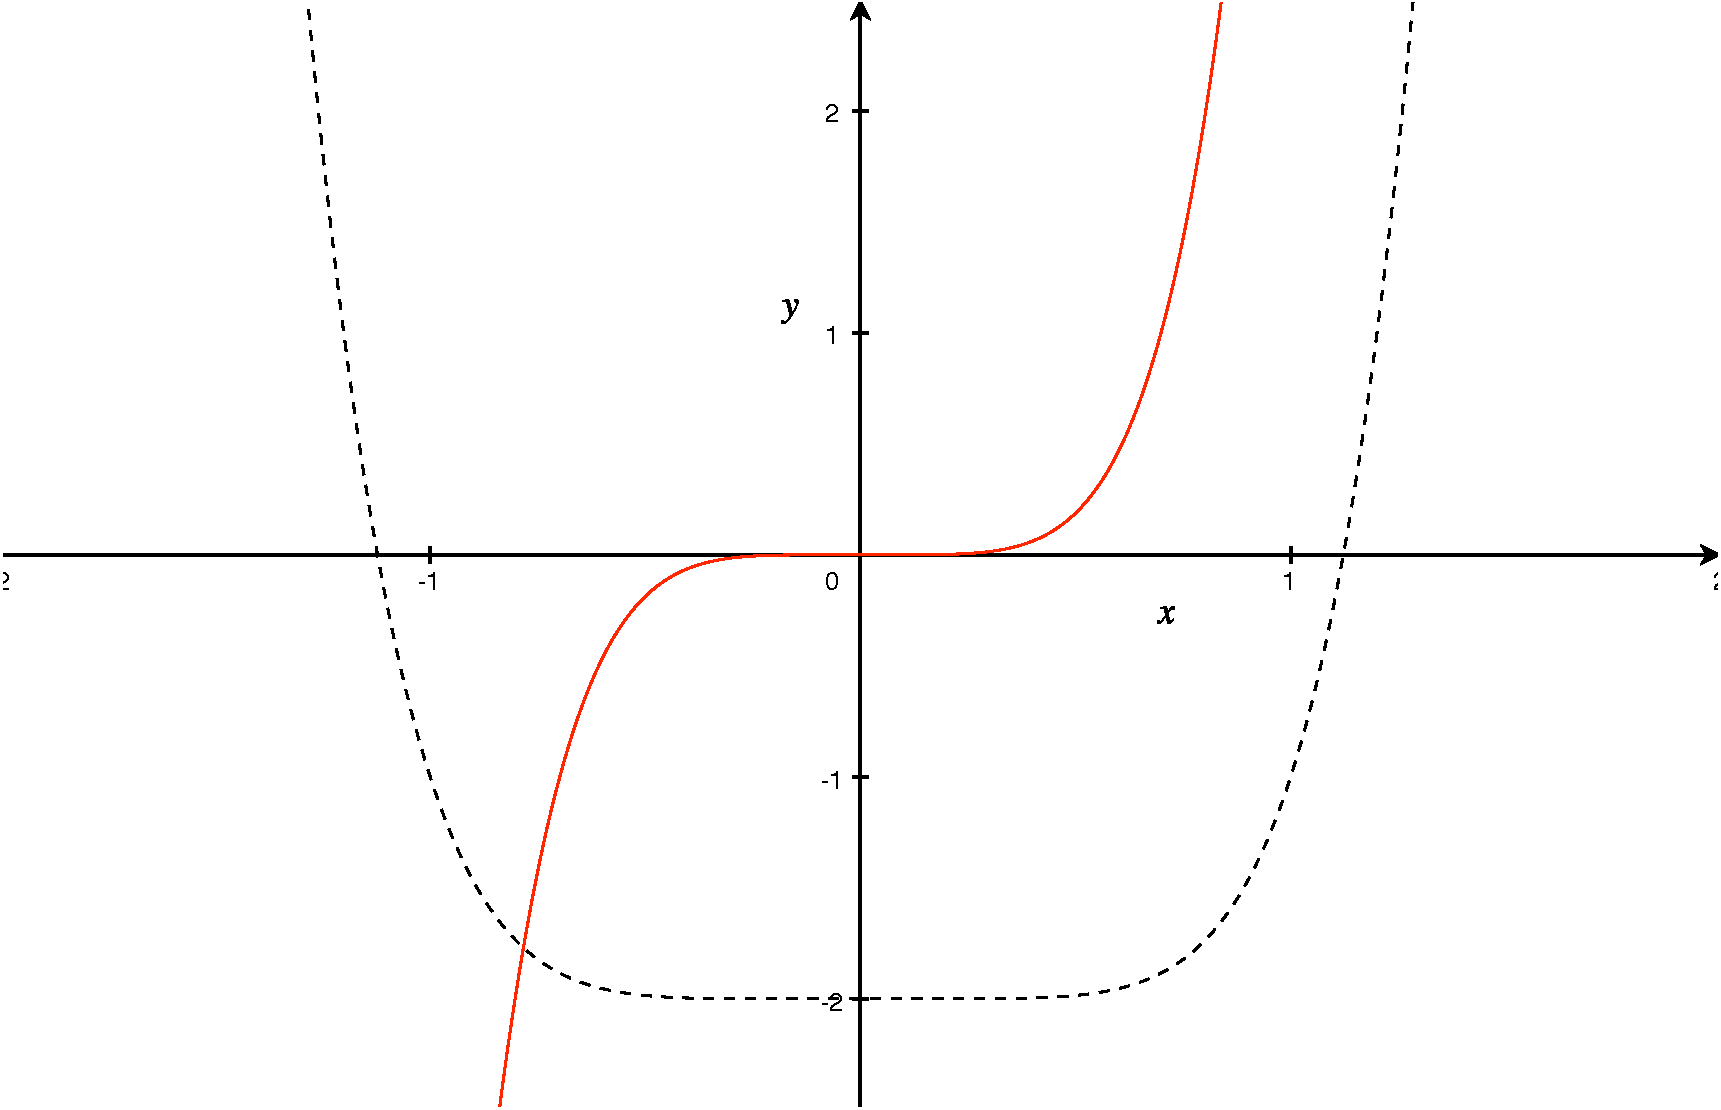
\includegraphics[width=5in]{./graphics/1722185.pdf} 
   \caption{WA-1722185}
   \label{fig:1722185}
\end{figure}
\begin{solution}
Work.
\end{solution}

\question 	%RogaCalcET2 3.2.051	WA-1722227

Find the point on the graph of $y = 5x^2 + 7x + 7$ at which the slope of the tangent line is equal to $2$.
\begin{solution}
Work.
\end{solution}

\question 	%RogaCalcET2 3.2.064	WA-1722219

Let $L$ be a tangent line to the hyperbola $xy = 1$ at $x = 3$. Find the area of the triangle bounded by $L$ and the coordinate axes.
 \begin{solution}
Work.
\end{solution}
 
\question 	%RogaCalcET2 3.2.084	WA-1731925

Consider the graph of $f\left(x\right) = 9 - x^2$. Find the coordinates of the point $P$ in the graph for which the tangent line passes through $\left(5, \ 0 \right)$.
\begin{solution}
Work.
\end{solution}
\begin{figure}[htbp] %  figure placement: here, top, bottom, or page
   \centering
   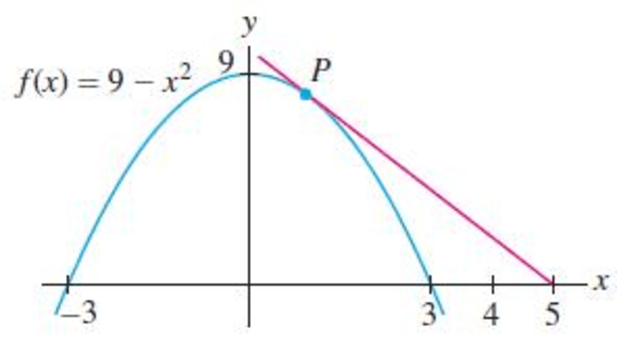
\includegraphics[width=5in]{./graphics/1731925.pdf} 
   \caption{WA-1731925}
   \label{fig:1731925}
\end{figure}

\end{questions}
\end{teacher}


\vfill
\pagebreak


%*-*-*-*-*-*-*-*-*-*-*-*-*-*-*-*-*-*-*-*-*-*-*-*-*-*-*-*-*-*-*-*-*-*-*-*-*-*-*-*-*-*-*-*-*-*-*-*-*-*-*-*-*-*-*-*-*-*-*-*-*-*-*-*-*-*-*-*-*-*-*-*-*-*-*-*-*-*-*-*-*-*-*-*-
\section{mth.121.03.03}
\subsection{Product and Quotient Rules}
\subsubsection{Product Rule}
The derivative of the product of two functions is the first function times the derivative of the second function plus the second function times the derivative of the first function.\footnote{A proof will be given in class.}
\[
\frac{{\rm{d}}}{{\rm{d}}x} \ \left[ f\left( x \right) \cdot g\left( x \right) \right]  = f\left( x \right) \cdot g'\left( x \right) + g\left( x \right) \cdot f'\left( x \right)
\]
\subsubsection{Quotient Rule}
The derivative of a quotient is the denominator times the derivative of the numerator minus the numerator times the derivative of the denominator; all divided by the square of the denominator.\footnote{A proof will not be given in class, but students are encouraged to try on their own.}
\[
\frac{{\rm{d}}}{{\rm{d}}x} \ \left[ \frac{f\left( x \right)}{g\left( x \right)} \right]  = \frac{g\left( x \right) \cdot f'\left( x \right) - f\left( x \right) \cdot g'\left( x \right)}{\left[ g\left( x \right)\right]^2} \]

\subsection{Examples}
\begin{questions}


\question Find $f'\left(x\right)$ by using the product rule.
\[
f\left(x\right) = e^{2x}
\]

\begin{solution}
You need to be able to show work on exams. Make sure you can follow the steps presented in class. Although I am providing the final answer, you should be aware that simplifications are not always necessary.
Final answer:
\[
f'\left(x\right) =  2 e^{2x}
\]
\end{solution}

\question Find $f'\left(x\right)$.\footnote{You should use the result from problem 1.}
\[
f\left(x\right) = \frac{1-x+x^2}{e^{2x}}
\]

\begin{solution}
You need to be able to show work on exams. Make sure you can follow the steps presented in class. Although I am providing the final answer, you should be aware that simplifications are not always necessary.
Final answer:
\[
f'\left(x\right) =  -\frac{2x^2-4x+3}{e^{2x}}
\]
\end{solution}

\question Find $f'\left(x\right)$.
\[
f\left(x\right) = \left(4e^x-x^2\right) \left(x^3-5\right)
\]

\begin{solution}
You need to be able to show work on exams. Make sure you can follow the steps presented in class. Although I am providing the final answer, you should be aware that simplifications are not always necessary.
Final answer:
\[
f'\left(x\right) =  4x^3 e^x + 12x^2 e^x - 20 e^x - 5x^4 + 10x
\]
\end{solution}

\question Find $f'\left(x\right)$.
\[
f\left(x\right) = \frac{x}{3x^2+1}
\]

\begin{solution}
You need to be able to show work on exams. Make sure you can follow the steps presented in class. Although I am providing the final answer, you should be aware that simplifications are not always necessary.
Final answer:
\[
f'\left(x\right) =  \frac{1-3x^2}{\left( 3x^2 + 1 \right)^2}
\]
\end{solution}

\question Find $f'\left(4\right)$.
\[
f\left(x\right) = \frac{\sqrt{x}+1}{\sqrt{x}-1}
\]

\begin{solution}
You need to be able to show work on exams. Make sure you can follow the steps presented in class. Although I am providing the final answer, you should be aware that simplifications are not always necessary.
Final answer:
\[
f'\left(x\right) =  - \frac{x \sqrt{x} + \sqrt{x} + 2x }{x \left( x-1\right)^2}, \quad f'\left(4\right) = -\frac{1}{2}
\]
\end{solution}

\question Find $f'\left(x\right)$.
\[
f\left(x\right) = x^2 e^{-x}
\]

\begin{solution}
You need to be able to show work on exams. Make sure you can follow the steps presented in class. Although I am providing the final answer, you should be aware that simplifications are not always necessary.
Final answer:
\[
f'\left(x\right) =  \frac{x\left( 2-x\right)}{e^x}
\]
\end{solution}

\question Find
\[
\left. \frac{{\rm{d}}y}{{\rm{d}}x} \right|_{x=0}, \quad y = \frac{3x^2+e^x-2}{4x^3+1}
\]

\begin{solution}
You need to be able to show work on exams. Make sure you can follow the steps presented in class. Although I am providing the final answer, you should be aware that simplifications are not always necessary.
Final answer:
\[
\left. \frac{{\rm{d}}y}{{\rm{d}}x} \right|_{x=0} = 1
\]
\end{solution}

\question Using the product rule to find $f'\left(x\right)$.
\[
f\left(x\right) = e^{3x}
\]
What do you think the derivative of $f\left(x\right) = e^{7x}$ is?

\begin{solution}
You need to be able to show work on exams. Make sure you can follow the steps presented in class. Although I am providing the final answer, you should be aware that simplifications are not always necessary.
Final answer:
\[
f'\left(x\right) =  3 e^{3x}
\]
The \emph{guess} for the derivative of $f\left(x\right) = e^{7x}$ is $f'\left(x\right) = 7e^{7x}$. 
\end{solution}


\end{questions}






\subsection{Assignment}
You should read \S  3.3 and do the WebAssign assignment mth.121.03.03.
\vfill
\pagebreak
%*-*-*-*-*-*-*-*-*-*-*-*-*-*-*-*-*-*-*-*-*-*-*-*-*-*-*-*-*-*-*-*-*-*-*-*-*-*-*-*-*-*-*-*-*-*-*-*-*-*-*-*-*-*-*-*-*-*-*-*-*-*-*-*-*-*-*-*-*-*-*-*-*-*-*-*-*-*-*-*-*-*-*-*-
\begin{teacher}
\subsection{Assessments}
The following questions are related to the WebAssign assignments and may be used to assess students' ability. Please do not share any of these questions with students.
\begin{questions}		
\question 	%RogaCalcET2 3.3.001	WA-1731878

Use the Product Rule to calculate the derivative.
\[
f \left( x \right) = x^3 \left( 6x^2 + 5 \right)
\]
\begin{solution}
Work
\end{solution}

\question 	%RogaCalcET2 3.3.003	WA-1731818

Use the Product Rule to calculate the derivative.
\[
f \left( x \right) = \left( x+5\right)^2 e^{\left(x+5\right)}
\]
\begin{solution}
Work
\end{solution}

\question 	%RogaCalcET2 3.3.005	WA-1731911

Use the Product Rule to calculate the derivative.
\[
h \left( s \right) = \left( s^{-1/2} + 2 s \right) \left( 7 - s^{-1} \right) 
\]
\begin{solution}
Work
\end{solution}

\question 	%RogaCalcET2 3.3.007	WA-1722642

Use the Quotient Rule to calculate the derivative for
\[
f\left(x\right) = \frac{4x}{2x- 2}.
\]
\begin{solution}
Work
\end{solution}


\question 	%RogaCalcET2 3.3.008	WA-1723877

Use the Quotient Rule to calculate the derivative for
\[
f\left(x\right) = \frac{x+7}{x^2+3x+1}.
\]
\begin{solution}
Work
\end{solution}

\question 	%RogaCalcET2 3.3.011	WA-1722665

Use the Quotient Rule to calculate the derivative for
\[
f\left(x\right) = \frac{12}{1 + e^{4x}}.
\]
\begin{solution}
Work
\end{solution}

\question 	%RogaCalcET2 3.3.016	WA-1722651


Calculate the derivative for
\[
f\left(x\right) = \frac{x^3 + 8x^2 + 5x^{-1}}{x}.
\]
\begin{solution}
Work
\end{solution}


\question 	%RogaCalcET2 3.3.020	WA-1756841

Calculate the derivative.
\[
z = \frac{x}{2x^2 + 1}
\]


\[
\left. \frac{{\rm{d}}z}{{\rm{d}}x} \right|_{x=-2} =
\]

\begin{solution}
Work
\end{solution}

\question 	%RogaCalcET2 3.3.026	WA-1760326

Calculate the derivative.
\[
f\left( x \right) = \frac{x^2 + 3x + 9}{\sqrt{x}}
\]
\begin{solution}
Work
\end{solution}

\question 	%RogaCalcET2 3.3.029	WA-1722629

Calculate the derivative for $f\left(x\right) = 5^{1/2}2^{1/2}$.

\begin{solution}
Work
\end{solution}

\question 	%RogaCalcET2 3.3.032	WA-1739576


Calculate the derivative.
\[
f\left(x\right) = x\left(x^2 + 6\right)\left(x + 6\right)
\]
\begin{solution}
Work
\end{solution}

\question 	%RogaCalcET2 3.3.037	WA-1722649

Calculate the following derivative. (Assume $a$ is a constant.)
\[
\frac{{\rm{d}}}{{\rm{d}}x} \left( \frac{ax-6}{x^5-a} \right)
\]


\begin{solution}
Work
\end{solution}

\question 	%RogaCalcET2 3.3.039	WA-1722620
Use the following function values
\[
f\left( 4 \right) = 4, \quad f'\left( 4 \right) = -9, \quad g\left( 4 \right) = 7, \quad g'\left( 4 \right) = -2,
\]
to find the derivative of $fg$ and $f/g$ at $x = 4$.

\begin{solution}
Work
\end{solution}

\question 	%RogaCalcET2 3.3.045	WA-1759098

Use the Product Rule to calculate 
\[
\frac{{\rm{d}}}{{\rm{d}}x} \left( e^{2x} \right)
\]
 
 \begin{solution}
Work
\end{solution}


\question 	%RogaCalcET2 3.3.046	WA-1755937

Let $f\left(x\right) = \displaystyle \frac{x}{x^2 + 2}$. Determine the intervals on which $f'\left(x\right) > 0$ and $f'\left(x\right) < 0$. (Enter your answers using interval notation.)

\begin{solution}
Work
\end{solution}
\end{questions}
\end{teacher}
\vfill
\pagebreak

%*-*-*-*-*-*-*-*-*-*-*-*-*-*-*-*-*-*-*-*-*-*-*-*-*-*-*-*-*-*-*-*-*-*-*-*-*-*-*-*-*-*-*-*-*-*-*-*-*-*-*-*-*-*-*-*-*-*-*-*-*-*-*-*-*-*-*-*-*-*-*-*-*-*-*-*-*-*-*-*-*-*-*-*-
\section{mth.121.03.04}
\subsection{Rates of Change}

\subsubsection{Velocity}

Recall that average velocity is
\[
\frac{\Delta s}{\Delta t},
\]
and when we let $\Delta t \to 0$ we get instantaneous velocity. It's really just the slope of the tangent line, so to get instantaneous velocity at time $t=a$, we need to evaluate the following limit.
\[
\mathop {\lim }\limits_{\Delta t \to 0 } \frac{\Delta s}{\Delta t} = \mathop {\lim }\limits_{t \to a } \frac{s\left(t\right) - s\left(a\right)}{t-a} =
\mathop {\lim }\limits_{h \to 0 } \frac{s\left(a + h\right) - s\left(a\right)}{h}.
\]



\textbf{Exapmle:} Find the instantaneous velocity at $t=3$ seconds, if the position (in meters) is related to time (in seconds) by
\[
s \left( t \right) = t^2-5t+3.
\]

\begin{solution}
Take the derivative,
\[
s' \left( t \right) = 2t-5,
\]
and evaluate this derivative at $t=3$,
\[
s' \left( 3 \right) = 1.
\]
So the answer is $1$ meter per second.
\end{solution}

\subsubsection{Rates in General}

Rates of changes don't necessarily have to be velocities. Here, using similar notation for a function $y = f\left(x\right)$, average rate of change is
\[
\frac{\Delta y}{\Delta x},
\]
and when we let $\Delta x \to 0$ we get instantaneous rate of change. It's really just the slope of the tangent line, so to get instantaneous rate at $x=a$, we need to evaluate the following limit.
\[
\mathop {\lim }\limits_{\Delta x \to 0 } \frac{\Delta y}{\Delta x} = \mathop {\lim }\limits_{x \to a } \frac{f\left(x\right) - f\left(a\right)}{x-a} =
\mathop {\lim }\limits_{h \to 0 } \frac{f\left(a + h\right) - f\left(a\right)}{h}.
\]



\textbf{Example:} Find the instantaneous rate of change of the cube root of $x$ with respect to $x$ when $x=8$. 

\begin{solution}
Here, we are  given that $f\left(x\right) = \sqrt[3]{x}$, and we're being asked to find $f'\left(8\right)$.
\begin{eqnarray*}
f\left(x\right) &=& \sqrt[3]{x}\\
f\left(x\right) &=& x^{1/3}\\
f'\left(x\right) &=& \frac{x^{-2/3}}{3}\\
f'\left(8\right) &=& \frac{8^{-2/3}}{3} = \frac{1}{12}
\end{eqnarray*}

\end{solution}



 
 
\subsection{Examples}
\begin{questions}
\question Find the rate of change of  the area of a square with respect to its side $s$ when $s=5$.
\begin{solution}
We'll discuss this in class.

\begin{eqnarray*}
A &=& s^2\\
\frac{{\rm{d}}A}{{\rm{d}}s} &=& 2s\\
\left. \frac{{\rm{d}}A}{{\rm{d}}s} \right|_{s=5}&=& 10\\
\end{eqnarray*}

\end{solution}


\question The position of a particle moving in a straight line during a five second trip is
\[
s\left(t\right) = t^2-t+10
\] centimeters. Find the time $t$ at which the instantaneous velocity is equal to the average velocity of the entire trip. 
\begin{solution}
We'll discuss this in class.

\begin{eqnarray*}
s\left(0\right) &=& 10\\
s\left(5\right) &=& 30\\
\frac{\Delta s}{\Delta t} &=& \frac{30 - 10}{5 - 0} = 4 \ \mbox{centimeters per second}\\
s' \left(t\right) &=& 2t-1\\
4 &=& 2t-1\\
t&=&2.5 \ \mbox{seconds}\\
\end{eqnarray*}

\end{solution}


\question A bullet is fired in the air vertically from two meters above ground level with an initial velocity of $200$ meters per second. Find the bullet's maximum velocity and maximum height.\footnote{Here we have
\[
s\left( t \right) = 2 + 200 t - \frac{9.8t^2}{2}.
\] You may recognize this formula if you've taken high-school level physics.}
\begin{solution}
We'll discuss this in class.

Final answer:

The maximum height is
\[
s\left( \frac{1000}{49} \right) = 2042.82 \ \mbox{meters}.
\]
And the maximum velocity is:
\[
s'\left( 40.8263  \right) = -200.098 \ \mbox{meters per second}.
\]
Realistically, this is really not true because we're neglecting many factors related to free falling bodies.
\end{solution}

\question A particle moving along a line has position $s\left(t\right) = t^4 - 8t^2$ feet, at time 
$t \geq 0$ seconds. What is the farthest distance to the left of the origin attained by the particle?
\begin{solution}
We'll discuss this in class.

Final answer:
\[
16 \ \mbox{feet}
\]
\end{solution}

\end{questions}









\subsection{Assignment}
You should read \S  3.4 and do the WebAssign assignment mth.121.03.04.
\vfill
\pagebreak
%*-*-*-*-*-*-*-*-*-*-*-*-*-*-*-*-*-*-*-*-*-*-*-*-*-*-*-*-*-*-*-*-*-*-*-*-*-*-*-*-*-*-*-*-*-*-*-*-*-*-*-*-*-*-*-*-*-*-*-*-*-*-*-*-*-*-*-*-*-*-*-*-*-*-*-*-*-*-*-*-*-*-*-*-
\begin{teacher}
\subsection{Assessments}
The following questions are related to the WebAssign assignments and may be used to assess students' ability. Please do not share any of these questions with students.
\begin{questions}		
\question 	%RogaCalcET2 3.4.001	WA-1755968

Find the rate of change. Area of a square with respect to its side $s$ when $s = 8$.


\question 	%RogaCalcET2 3.4.004	WA-1755971

Find the rate of change of the reciprocal $1/x$ with respect to $x$ when $x = 39$, $40$, and $41$.
\begin{parts}
\part $f'\left(39\right)=$
\part $f'\left(40\right)=$
\part $f'\left(41\right)=$
\end{parts}
 
 
 
\question 	%RogaCalcET2 3.4.009a	WA-1761049

The graph of distance $s\left(t\right)$ from the origin as a function of time for a car trip is given:
 \begin{figure}[htbp] %  figure placement: here, top, bottom, or page
    \centering
    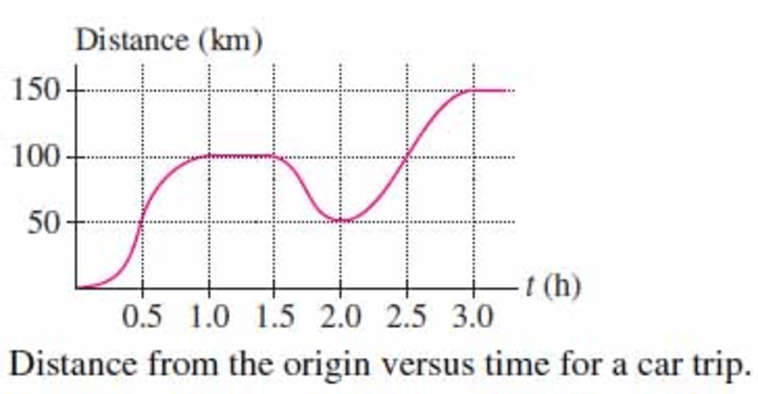
\includegraphics[width=3in]{./graphics/1761049.pdf} 
    \caption{WA-1761049}
    \label{fig:1761049}
 \end{figure}

Find the average velocity over the interval.
\[
\left[0, \ 1 \right]
\]

\question 	%RogaCalcET2 3.4.011a	WA-1761081

Consider the graph for the distance from the origin versus time for a car trip.
The graph of distance $s\left(t\right)$ from the origin as a function of time for a car trip is given:
 \begin{figure}[htbp] %  figure placement: here, top, bottom, or page
    \centering
    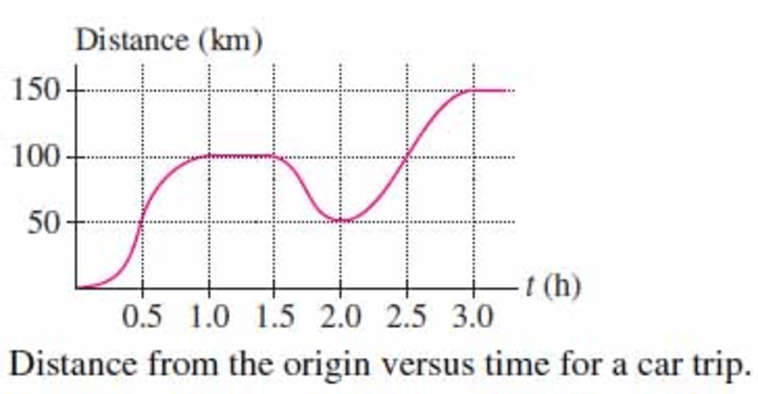
\includegraphics[width=3in]{./graphics/1761049.pdf} 
    \caption{WA-1761081}
    \label{fig:1761049}
 \end{figure}
Identify the correct statement (circle one) for the given interval.
\[
\left[ 0.5, \ 1.0 \right]
\]

\begin{parts}
\part The velocity is increasing.
\part The velocity is decreasing.    
\part The velocity is negative.
\part The velocity remains constant.
\part The car is stopped.
\end{parts}

\question 	%RogaCalcET2 3.4.014	WA-1761172

The temperature (in centigrade) of an object at time $t$ (in minutes) is
\[ 
T\left(t\right) = \frac{3}{8} t^2 - 15t + 240
\]
for $0 \leq  t \leq ≤ 20$. At what rate is the object cooling at $t = 10$?



\question 	%RogaCalcET2 3.4.037	WA-1761072

The tangent lines to the graph of $f\left(x\right) = 7x^2$ grow steeper as $x$ increases. At what rate do the slopes of the tangent lines increase?
 
\question 	%RogaCalcET2 3.4.024	WA-1761071

A particle moving along a line has position $s\left(t\right) = t^4 - 72t^2$ m, at time $t$seconds. What is the farthest distance to the left of the origin attained by the particle?

\end{questions}
\end{teacher}
\vfill
\pagebreak


%*-*-*-*-*-*-*-*-*-*-*-*-*-*-*-*-*-*-*-*-*-*-*-*-*-*-*-*-*-*-*-*-*-*-*-*-*-*-*-*-*-*-*-*-*-*-*-*-*-*-*-*-*-*-*-*-*-*-*-*-*-*-*-*-*-*-*-*-*-*-*-*-*-*-*-*-*-*-*-*-*-*-*-*-
\section{mth.121.03.05}
\subsection{Higher Order Derivatives}


The first derivative is often indicated using \emph{pime} notation, for example if we have a function $f\left(x\right)$, we write $f'\left(x\right)$ to indicate
\[
\frac{{\rm{d}}}{{\rm{d}}x}\left[f\left(x\right)\right].
\]
Continuing with this notation, we can take derivatives of derivatives. So the second derivative would be indicated by
\[
f''\left(x\right) = \frac{{\rm{d}}}{{\rm{d}}x}\left[f'\left(x\right)\right].
\]
And the third derivative,
\[
f'''\left(x\right) = \frac{{\rm{d}}}{{\rm{d}}x}\left[f''\left(x\right)\right].
\]
The \emph{pime} notation usually stops at order three, but we can still continue,  this time we use a superscript in parentheses to indicate the order. For example the forth derivative would be indicated by
\[
f^{\left(4\right)}\left(x\right) = \frac{{\rm{d}}}{{\rm{d}}x}\left[f'''\left(x\right)\right].
\]
In general, if $y=f\left(x\right)$, we write the derivatives as follows.
\begin{align*}
f'\left( x \right)  = y' &= \frac{{\rm{d}}y}{{\rm{d}}x} & \text{first derivative}\\
f''\left( x \right) = y'' &= \frac{{\rm{d}}^2y}{{\rm{d}}x^2} & \text{second derivative}\\
f'''\left( x \right) = y''' &= \frac{{\rm{d}}^3y}{{\rm{d}}x^3} & \text{third derivative}\\
f^{\left(4\right)}\left( x \right) = y^{\left(4\right)}  &= \frac{{\rm{d}}^4y}{{\rm{d}}x^4} & \text{fourth derivative}\\
\vdots &= \vdots  & \\
f^{\left(n\right)}\left( x \right) = y^{\left(n\right)}&= \frac{{\rm{d}}^n y}{{\rm{d}}x^n} & \text{$n^{\rm{th}}$ derivative}
\end{align*}
Since derivatives tell us how something changes, you can probably reason that the second derivative tells us how fast the first derivative is changing, and so forth and so on. As we start using derivatives, these relationships should become better understood.
\subsection{Examples}
\begin{questions}
\question Find $y'$ and $y''$.
\[
y = \frac{1}{1-x}
\]

\begin{solution}
We'll discuss this in class.
\begin{eqnarray*}
y &=& \frac{1}{1-x}\\
y' &=& \frac{1}{\left( 1-x \right)^{2}} = \left( 1-x \right)^{-2}\\
y'' &=& \frac{2}{\left( 1-x \right)^{3}} = 2 \left( 1-x \right)^{-3}
\end{eqnarray*}

\end{solution}

\question Find $h''\left(3\right)$.
\[
h\left(t\right) = \frac{e^t}{t}
\]

\begin{solution}
We'll discuss this in class.
\begin{eqnarray*}
h\left(t\right) &=& \frac{e^t}{t}\\
h'\left(t\right) &=& \frac{t e^t - e^t}{t^2}\\
h''\left(t\right) &=& \frac{t^2 e^t - 2t e^t + 2e^t}{t^3}\\
h''\left(3\right) &=& \frac{5e^3}{27} \approx 3.71954
\end{eqnarray*}

\end{solution}

\question Find a formula\footnote{The factorial notation ($n!$) was introduced in MTH 120 and your answer should include a factorial.} for $f^{\left(n\right)}\left(x\right)$.
\[
f\left(x\right) = x^{-2}
\]

\begin{solution}
We'll discuss this in class. Final answer:
\[
f^{\left(n\right)}\left(x\right) =  \left( -1 \right)^{n} \frac{\left( n + 1 \right)!}{x^{n+2}}
\]
\end{solution}

\question The graph (Figure \ref{fig:graph1301}, page \pageref{fig:graph1301}) below shows $f$, $f'$, $f''$. Determine which is which.

\begin{figure}[htbp] %  figure placement: here, top, bottom, or page
   \centering
   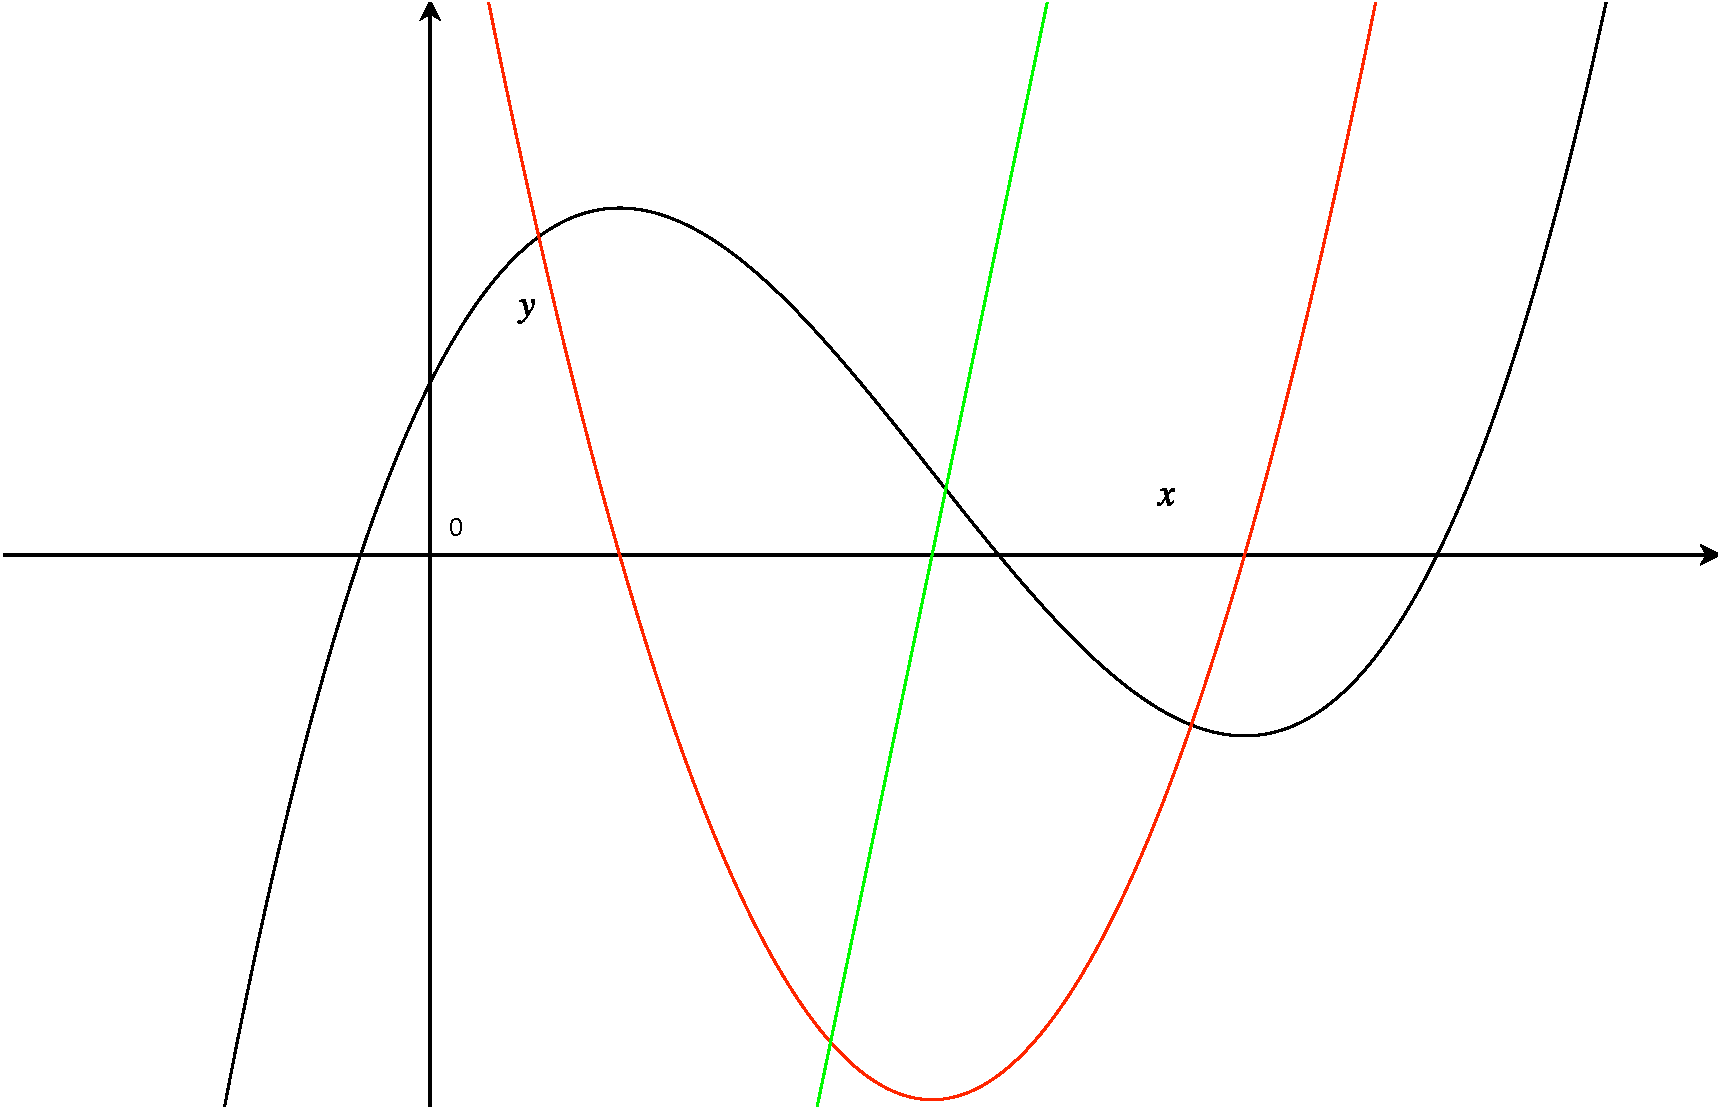
\includegraphics[width=4in]{./graphics/graph1301.pdf} 
   \caption{Partial graph of $f$, $f'$, $f''$.}
   \label{fig:graph1301}
\end{figure}

\begin{solution}
We'll discuss this in class.
The black curve is $f$, the red curve is $f'$ and green curve is $f''$.
\end{solution}

\end{questions}



















\subsection{Assignment}
You should read \S  3.5 and do the WebAssign assignment mth.121.03.05.
\vfill
\pagebreak
%*-*-*-*-*-*-*-*-*-*-*-*-*-*-*-*-*-*-*-*-*-*-*-*-*-*-*-*-*-*-*-*-*-*-*-*-*-*-*-*-*-*-*-*-*-*-*-*-*-*-*-*-*-*-*-*-*-*-*-*-*-*-*-*-*-*-*-*-*-*-*-*-*-*-*-*-*-*-*-*-*-*-*-*-
\begin{teacher}
\subsection{Assessments}
The following questions are related to the WebAssign assignments and may be used to assess students' ability. Please do not share any of these questions with students.
\begin{questions}		
\question 	%RogaCalcET2 3.5.001	WA-1722700


Calculate the first, second and third derivatives of $y = 4x^7$.
\begin{parts}
\part $y'=$
\begin{solution}
Work
\end{solution}
\part $y''=$
\begin{solution}
Work
\end{solution}
\part $y'''=$
\begin{solution}
Work
\end{solution}
\end{parts}

\question 	%RogaCalcET2 3.5.004	WA-1722703

Calculate the first, second and third derivatives of $y = 5x^3 - 8x^2 + 7$.
\begin{parts}
\part $y'=$
\begin{solution}
Work
\end{solution}
\part $y''=$
\begin{solution}
Work
\end{solution}
\part $y'''=$
\begin{solution}
Work
\end{solution}
\end{parts}


\question 	%RogaCalcET2 3.5.009	WA-1761169

Calculate the second and third derivatives of
\[
y = z - \frac{3}{z}.
\]
\begin{parts}
\part $y''=$
\begin{solution}
Work
\end{solution}
\part $y'''=$
\begin{solution}
Work
\end{solution}
\end{parts}


\question 	%RogaCalcET2 3.5.013	WA-1761158

Calculate the second and third derivatives of
\[
y = \frac{7x-7}{x}.
\]
\begin{parts}
\part $y''=$
\begin{solution}
Work
\end{solution}
\part $y'''=$
\begin{solution}
Work
\end{solution}
\end{parts}

\question 	%RogaCalcET2 3.5.014	WA-1722721

Calculate the first, second and third derivatives of
\[
y = \frac{4}{3+x}.
\]
\begin{parts}
\part $y'=$
\begin{solution}
Work
\end{solution}
\part $y''=$
\begin{solution}
Work
\end{solution}
\part $y'''=$
\begin{solution}
Work
\end{solution}
\end{parts}

\question 	%RogaCalcET2 3.5.015	WA-1724763

Calculate the first, second and third derivatives of $y = x^6e^x$.
\begin{parts}
\part $y'=$
\begin{solution}
Work
\end{solution}
\part $y''=$
\begin{solution}
Work
\end{solution}
\part $y'''=$
\begin{solution}
Work
\end{solution}
\end{parts}

\question 	%RogaCalcET2 3.5.020	WA-1722699

Calculate the following derivative if $f\left(x\right) = 6x^8  - 2x^7$.
\[
\left. \frac{{\rm{d}}^4f}{{\rm{d}}x^4} \right|_{x=1} =
\]
\begin{solution}
Work
\end{solution}

\question 	%RogaCalcET2 3.5.025	WA-1761031

Calculate the derivative indicated.
\[
h\left(w\right) = \sqrt{w} e^w, \quad h''\left( 1 \right) =
\]
\begin{solution}
Work
\end{solution}

\question 	%RogaCalcET2 3.5.028	WA-1739548

Which of the following functions satisfy $f^{\left(k\right)} \left(x\right) = 0$ for all $k \geq 6$? Select all that apply.
\begin{parts}
\part $5x^4+3x+x^{-1}$
\begin{solution}
Work
\end{solution}
\part $x^3-3$
\begin{solution}
Work
\end{solution}
\part $\sqrt{x}$
\begin{solution}
Work
\end{solution}
\part $5-x^6$
\begin{solution}
Work
\end{solution}
\part $x^{9/5}$
\begin{solution}
Work
\end{solution}
\part $8x^2+6x^5$
\begin{solution}
Work
\end{solution}
\end{parts}

\question 	%RogaCalcET2 3.5.037a	WA-1761100

Find the acceleration at time $t = 5$ min of a helicopter whose height is $h\left(t\right) = -3t^3 + 600t$ feet.
\begin{solution}
Work
\end{solution}


\question 	%RogaCalcET2 3.5.037b	WA-1761512

At time $t = 5$ min of the flight of a helicopter whose height is $h\left(t\right) = 300t - 3t^3$ feet the velocity is $v\left(t\right) = h'\left(t\right) = 300 - 9t^2$ and acceleration is $a\left(t\right) = h''\left(t\right) = -18t$. Thus $a\left(5\right) = -90$ ft/min$^2$. Consider the graph below.
\begin{figure}[htbp] %  figure placement: here, top, bottom, or page
   \centering
   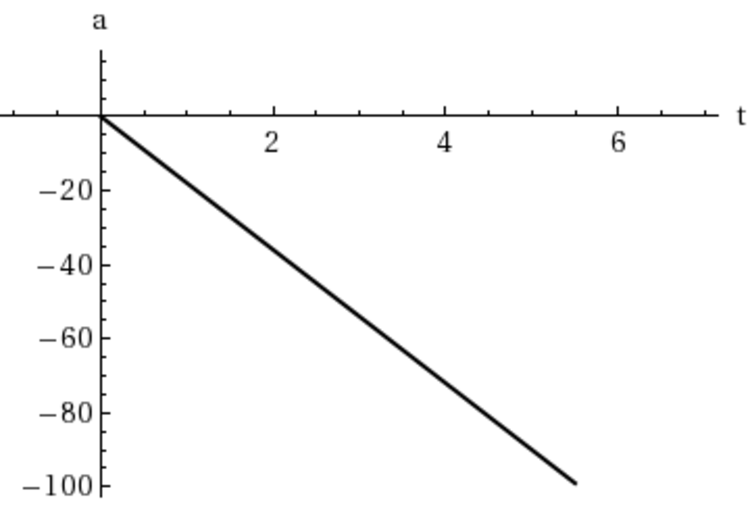
\includegraphics[width=2in]{./graphics/1761512.pdf} 
   \caption{	WA-1761512}
   \label{fig:1761512}
\end{figure}
Since velocity is positive in this time interval, does this graph show that the helicopter is slowing down during this time interval? Circle Yes of No.
\begin{solution}
Work
\end{solution}


\question 	%RogaCalcET2 3.5.039	WA-1724760

The figure below shows $f$, $f'$, and $f''$. Determine which is which.
\begin{figure}[htbp] %  figure placement: here, top, bottom, or page
   \centering
   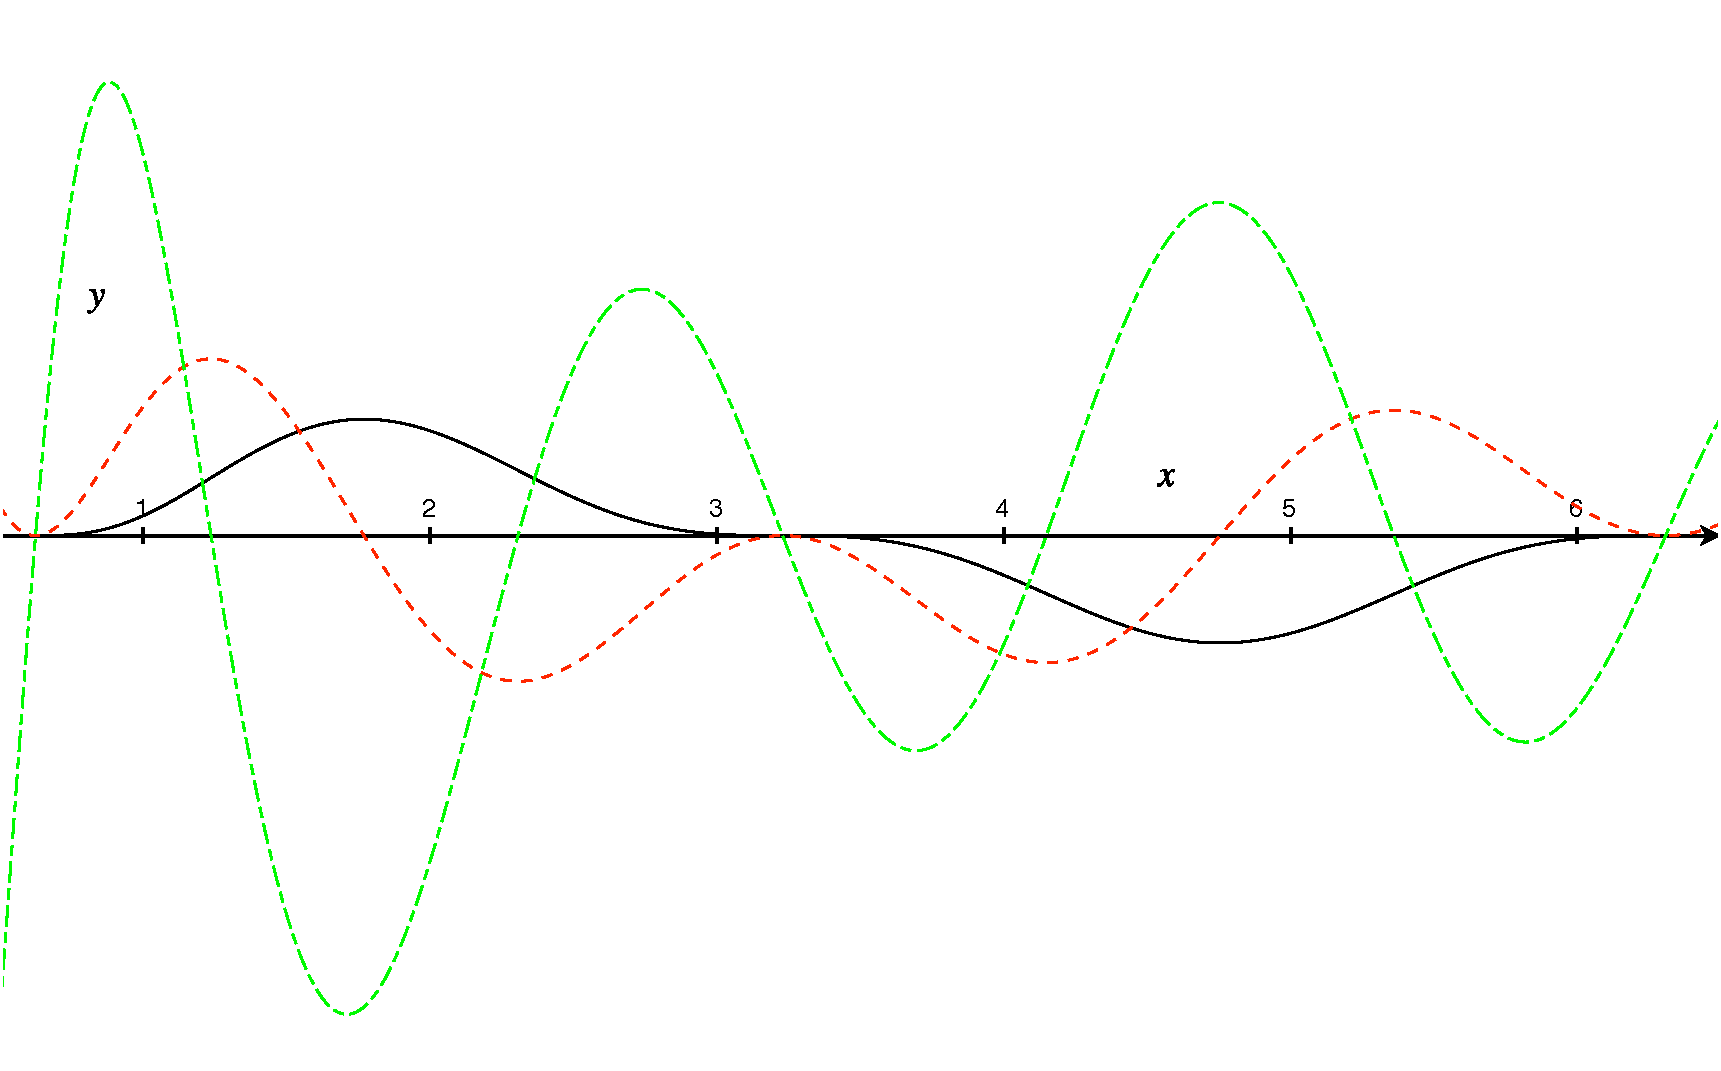
\includegraphics[width=3in]{./graphics/1724760.pdf} 
   \caption{WA-1724760}
   \label{fig:1724760}
\end{figure}
\begin{solution}
Work
\end{solution}
\question 	%RogaCalcET2 3.5.043	WA-1722691

Find a value of $n$ such that $y = x^ne^x$ satisfies the equation $xy' = \left(x - 7\right)y$.

\begin{solution}
Work
\end{solution}
\question 	%RogaCalcET2 3.5.051	WA-1761076

Let $f\left(x\right) = \displaystyle \frac{x+4}{x-27}$. Use a computer algebra system to compute the $f^{\left(k\right)}\left(x\right)$ for $1 \leq k \leq 4$. Find a general formula for $f^{\left(k\right)}\left(x\right)$.
\begin{solution}
Work
\end{solution}

\end{questions}
\end{teacher}
\vfill
\pagebreak

%*-*-*-*-*-*-*-*-*-*-*-*-*-*-*-*-*-*-*-*-*-*-*-*-*-*-*-*-*-*-*-*-*-*-*-*-*-*-*-*-*-*-*-*-*-*-*-*-*-*-*-*-*-*-*-*-*-*-*-*-*-*-*-*-*-*-*-*-*-*-*-*-*-*-*-*-*-*-*-*-*-*-*-*-
\section{mth.121.03.06}
\subsection{Trigonometric Derivatives}

The definition of the \emph{derivative as a function} is,
\[
f' \left( x \right) = \mathop {\lim }\limits_{h \to 0 }  \frac{f \left( x+h \right) - f \left( x \right)}{h},
\]
provided the limit exists.\footnote{Now of course our new function will have a domain that may differ from the originating function. Yes, the derivative may not be defined at all points along the function.} Okay, I'm being repetitious here, but it is nonetheless necessary to be reminded of this definition before proceeding forward.


\subsubsection{The Derivative of Sine}


I'd like to show that the derivative of the sine function is the cosine function. Showing that this is the case is not difficult. First, draw (Figure \ref{fig:graph1401}, page \pageref{fig:graph1401}) one cycle of the sine function, and it's derivative\footnote{Same method that we're doing in class. That is, try to find the slopes at some points and then connect the dots.} on the same graph.
\begin{figure}[htbp] %  figure placement: here, top, bottom, or page
   \centering
   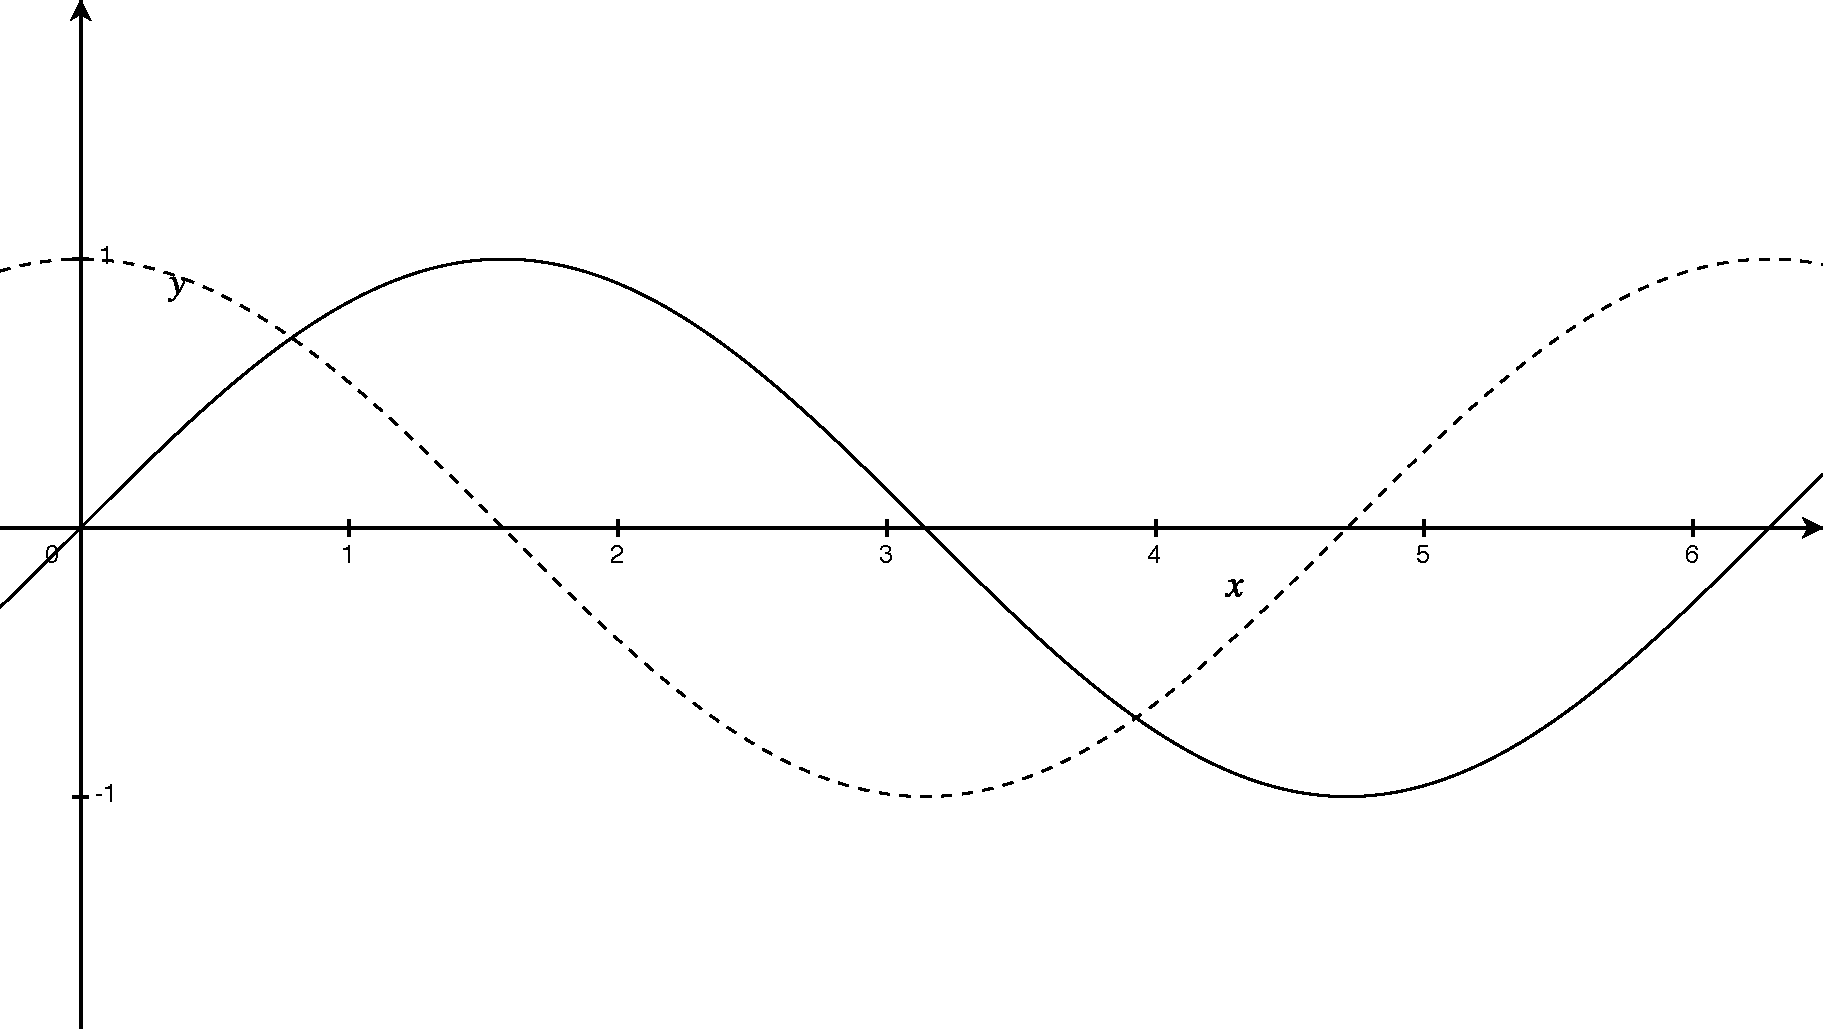
\includegraphics[width=4in]{./graphics/graph1401.pdf} 
   \caption{The sine function (solid) and its derivative (dashed).}
   \label{fig:graph1401}
\end{figure}

You should observe that the dashed curve looks like the cosine curve, but this is certainly not a proof, but at least it's giving us a hint.



To find the derivative of the sine function we will need to use the definition of derivative.
\begin{eqnarray*}
\frac{{\rm{d}}}{{\rm{d}}x} \left( \sin x \right) &=& \mathop {\lim }\limits_{ h \to 0} \frac{\sin \left( x + h \right) - \sin x}{h}
\end{eqnarray*}
This limit does not look easy, and you may wonder why its being rewritten in this form.\footnote{The main reason is that this is what you did in MTH-120, and sum identities were extensively used.}
\begin{eqnarray*}
\frac{{\rm{d}}}{{\rm{d}}x} \left( \sin x \right) &=& \mathop {\lim }\limits_{ h \to 0} \frac{\sin \left( x + h \right) - \sin x}{h}\\
&=& \mathop {\lim }\limits_{ h \to 0} \frac{\sin x \cos h + \sin h \cos x - \sin x}{h}\\
&=& \mathop {\lim }\limits_{ h \to 0} \left[\frac{\sin x \cos h - \sin x}{h} + \frac{\sin h \cos x}{h}\right]\\
&=& \mathop {\lim }\limits_{ h \to 0} \left[\sin x \cdot \frac{ \cos h - 1}{h} + \cos x \cdot \frac{\sin h }{h}\right]
\end{eqnarray*}
Wow, I've seen\footnote{Look back over your notes if necessary.} both of these limits before.
\[
\mathop {\lim }\limits_{ h \to 0} \frac{\sin h }{h} = 1, \qquad \mathop {\lim }\limits_{ h \to 0} \frac{ \cos h - 1}{h} = 0
\]
Continuing from above, we have:
\begin{eqnarray*}
\frac{{\rm{d}}}{{\rm{d}}x} \left( \sin x \right) &=& \mathop {\lim }\limits_{ h \to 0} \left[\sin x \cdot \frac{ \cos h - 1}{h} + \cos x \cdot \frac{\sin h }{h}\right]\\
&=& \mathop {\lim }\limits_{ h \to 0} \sin x \cdot \frac{ \cos h - 1}{h} +  \mathop {\lim }\limits_{ h \to 0}  \cos x \cdot \frac{\sin h }{h}\\
&=& \sin x \cdot \mathop {\lim }\limits_{ h \to 0}  \frac{ \cos h - 1}{h} +  \cos x \cdot \mathop {\lim }\limits_{ h \to 0}   \frac{\sin h }{h}\\
&=& \sin x \cdot 0 +  \cos x \cdot 1\\
&=& \cos x
\end{eqnarray*}



 
 
\subsection{Examples}

\begin{questions}
\question You \emph{should} be able to prove using the definition of the derivative that
\[
\frac{{\rm{d}}}{{\rm{d}}x} \left( \cos x \right) = -\sin x,
\]

\begin{solution} This will be discussed in class.
\begin{eqnarray*}
\frac{{\rm{d}}}{{\rm{d}}x} \left( \cos x \right) &=& \mathop {\lim }\limits_{ h \to 0} \frac{\cos \left( x + h \right) - \cos x}{h}\\
&=& \mathop {\lim }\limits_{ h \to 0} \frac{\cos x \cos h - \sin x \sin h - \cos x}{h}\\
&=& \mathop {\lim }\limits_{ h \to 0} \left[\frac{\cos x \cos h - \cos x}{h} - \frac{\sin x \sin h}{h}\right]\\
&=& \mathop {\lim }\limits_{ h \to 0} \left[\cos x \cdot \frac{ \cos h - 1}{h} - \sin x \cdot \frac{\sin h }{h}\right]\\
&=& -\sin x
\end{eqnarray*}
\end{solution}

\question Using rules you should be able to show that
\[
\frac{{\rm{d}}}{{\rm{d}}x} \left( \tan x \right) = \sec^2 x.
\]

\begin{solution}
This will be discussed in class.
\begin{eqnarray*}
\frac{{\rm{d}}}{{\rm{d}}x} \left( \tan x \right) &=& \frac{{\rm{d}}}{{\rm{d}}x} \left( \frac{\sin x }{\cos x} \right)\\
&=& \frac{\cos^2 x + \sin^2 x}{\cos^2 x}\\
&=& \sec^2 x
\end{eqnarray*}
\end{solution}

\question Using rules you should be able to show that
\[
\frac{{\rm{d}}}{{\rm{d}}x} \left( \csc x \right) = -\cot x \csc x.
\]

\begin{solution}
You should be able to do this on your own now, especially after seeing the last example. And again, we'll do this in class.
\end{solution}

\question Using rules you should be able to show that
\[
\frac{{\rm{d}}}{{\rm{d}}x} \left( \sec x \right) = \tan x \sec x.
\]

\begin{solution}
You should be able to do this on your own now, especially after seeing the last example. And again, we'll do this in class.
\end{solution}

\question Using rules you should be able to show that
\[
\frac{{\rm{d}}}{{\rm{d}}x} \left( \cot x \right) = -\csc^2 x.
\]

\begin{solution}
You should be able to do this on your own now, especially after seeing the last example. And again, we'll do this in class.
\end{solution}

\question Find an equation of the tangent line to the curve $y = \sec x - 2 \cos x$ at the point $\left( \pi/3, \ 1\right)$.

\begin{solution}
We'll discuss this in class.

Final answer:
\[
y-1=3\sqrt{3} \left(x-\frac{\pi}{3} \right)
\]
\end{solution}

\question Differentiate.
\[
y = \frac{x + \sin x}{x^2+ \cos x}
\]

\begin{solution}
We'll discuss this in class.

Final answer:
\[
y' \left( x \right) = \frac{1 - x^2 - x \sin x + \left( x^2 + 1 \right) \cos x}{\left( x^2+ \cos x \right)^2}
\]
\end{solution}

\question Find the limit.
\[
\mathop {\lim }\limits_{x \to 0} \frac{\sin^2 3x }{ x^2}
\]

\begin{solution}
We'll discuss this in class.

Final answer:
\[
\mathop {\lim }\limits_{x \to 0} \frac{\sin^2 3x }{ x^2} = 9
\]
\end{solution}

\question Find the limit.
\[
\mathop {\lim }\limits_{x \to 0} \frac{1 - \tan x}{ \sin x - \cos x}
\]


\begin{solution}
We'll discuss this in class.

Final answer:
\[
\mathop {\lim }\limits_{x \to 0} \frac{1 - \tan x}{ \sin x - \cos x} =-1
\]
\end{solution}


\question Suppose $f\left( \pi / 3 \right) = 4$ and $f'\left( \pi / 3 \right) = -2$, and let $g\left( x \right) = f\left( x \right) \sin x$ and $h\left( x \right) = \cos x \ \div \ f\left( x \right)$. Find $g'\left( \pi / 3 \right)$ and $h'\left( \pi / 3 \right)$.

\begin{solution}
We'll discuss this in class.

Final answers:
\begin{eqnarray*}
g'\left( \pi / 3 \right) &=& 2 - \sqrt{3}\\
h'\left( \pi / 3 \right) &=& \frac{1 - 2\sqrt{3} }{16}
\end{eqnarray*}

\end{solution}

\question If $f\left( \beta \right) = \beta \cdot \sin \beta$, find $f'\left( \beta \right)$ and $f''\left( \beta \right)$.

\begin{solution}
We'll discuss this in class.

Final answers:
\begin{eqnarray*}
f'\left( \beta \right) &=& \sin \beta + \beta  \cos \beta\\
f''\left( \beta \right) &=& 2  \cos \beta - \beta  \sin \beta
\end{eqnarray*}
\end{solution}



\end{questions}
















\subsection{Assignment}
You should read \S  3.6 and do the WebAssign assignment mth.121.03.06.
\vfill
\pagebreak
%*-*-*-*-*-*-*-*-*-*-*-*-*-*-*-*-*-*-*-*-*-*-*-*-*-*-*-*-*-*-*-*-*-*-*-*-*-*-*-*-*-*-*-*-*-*-*-*-*-*-*-*-*-*-*-*-*-*-*-*-*-*-*-*-*-*-*-*-*-*-*-*-*-*-*-*-*-*-*-*-*-*-*-*-
\begin{teacher}
\subsection{Assessments}
The following questions are related to the WebAssign assignments and may be used to assess students' ability. Please do not share any of these questions with students.
\begin{questions}		
\question 	%RogaCalcET2 3.6.002	WA-1722704

Find an equation of the tangent line to $y = 3 \cos x$ at $x = \pi/3$.
\begin{solution}
Work
\end{solution}

\question 	%RogaCalcET2 3.6.006	WA-1739608

Find the derivative of $f\left(x\right) = 2x^2 \sin x + 2x \cos x$.
\begin{solution}
Work
\end{solution}

\question 	%RogaCalcET2 3.6.011	WA-1724784

Find the derivative of $f\left(x\right) = 5 \tan x \ \sec x$.
\begin{solution}
Work
\end{solution}

\question 	%RogaCalcET2 3.6.012	WA-1722947

Find the derivative of $f\left(x\right) = x^4 \sin^3 x$.
\begin{solution}
Work
\end{solution}

\question 	%RogaCalcET2 3.6.014	WA-1724764

Find the derivative of $f\left(x\right) = 9x \tan x$.
\begin{solution}
Work
\end{solution}

\question 	%RogaCalcET2 3.6.017	WA-1737543

Compute the derivative.
\[
R\left(y\right) =  \frac{10 \cos y - 11}{\sin y}
\]
\begin{solution}
Work
\end{solution}
\question 	%RogaCalcET2 3.6.019	WA-1722953

Find the derivative of $f\left(x\right) = 2 \sin x - \displaystyle \frac{6}{\cos x}$.
\begin{solution}
Work
\end{solution}

\question 	%RogaCalcET2 3.6.028	WA-1737501

Find an equation of the tangent line at the point specified.
\[
y = \frac{\sin t}{4 + 4 \cos t}, \quad t = \frac{\pi}{3}
\]
\begin{solution}
Work
\end{solution}
\question 	%RogaCalcET2 3.6.031	WA-1724792

Find an equation of the tangent line to $y = 4e^x \cos x$ at $x = 0$.
\begin{solution}
Work
\end{solution}

\question 	%RogaCalcET2 3.6.038	WA-1755943

\begin{parts}
\part If $y = \sin \left( x + 15\right)$, does $y'' = - y$?
\begin{solution}
Work
\end{solution}
\part If $y = \cos \left( x + 15\right)$, does $y'' = - y$?
\begin{solution}
Work
\end{solution}
\end{parts}

\question 	%RogaCalcET2 3.6.042	WA-1741301

Calculate the higher derivatives.
\[
y = 5e^t \sin t
\]
\begin{parts}
\part $y'' = $
\begin{solution}
Work
\end{solution}
\part $y''' = $
\begin{solution}
Work
\end{solution}
\end{parts}

\question 	%RogaCalcET2 3.6.043	WA-1739521

Use the function given below to answer the following questions.
\[
f \left( x \right) = \sin x
\]

\begin{parts}
\part $f' = $
\begin{solution}
Work
\end{solution}
\part $f'' = $
\begin{solution}
Work
\end{solution}
\part $f''' = $
\begin{solution}
Work
\end{solution}
\part $f^{\left(4\right)} = $
\begin{solution}
Work
\end{solution}
\part $f^{\left(5\right)} = $
\begin{solution}
Work
\end{solution}
\part $f^{\left(8\right)} = $
\begin{solution}
Work
\end{solution}
\part $f^{\left(36\right)} = $
\begin{solution}
Work
\end{solution}
\end{parts}
\end{questions}
\end{teacher}
\vfill
\pagebreak


%*-*-*-*-*-*-*-*-*-*-*-*-*-*-*-*-*-*-*-*-*-*-*-*-*-*-*-*-*-*-*-*-*-*-*-*-*-*-*-*-*-*-*-*-*-*-*-*-*-*-*-*-*-*-*-*-*-*-*-*-*-*-*-*-*-*-*-*-*-*-*-*-*-*-*-*-*-*-*-*-*-*-*-*-
\section{mth.121.03.07}
\subsection{The Chain Rule}


\subsubsection{Local Linearization}

In class I derived some of the simple rules for differentiation. The technique we used is exactly the same one that is used in the most textbooks. Now I'd like to use the concept of local linearization to derive the chain rule. We will still use the definition of the derivative, but now we will use the local linearization\footnote{This concept will be discussed in class and is basically using an equation of a tangent line, in a local region, to approximate the curve. Actually for very small $h \neq 0$ we have
\[
\frac{f \left( x + h \right) - f \left( x\right)}{h} \approx f' \left( x\right) \quad \Rightarrow \quad f \left( x + h \right) \approx f \left( x  \right) + f' \left( x  \right) h.
\]} as follows,
\[
f \left( x + h \right) \approx f \left( x  \right) + f' \left( x  \right) h,
\]
and
\[
g \left( x + h \right) \approx g \left( x  \right) + g' \left( x  \right) h.
\]
The smaller $h$ gets, the better these approximations become. In fact if we take the limit of each side, as $h \rightarrow 0$, we get an equality. As a simple example, let's derive the product rule using these local linearization along with the definition of derivative.
\begin{eqnarray*}
\left[ f \left( x \right)  g \left( x \right) \right]' &=&
\mathop {\lim }\limits_{h \to 0 }  
\frac{f \left( x+h \right)  g \left( x+h \right) - f \left( x \right)  g \left( x \right) }{h}\\
&=&
\mathop {\lim }\limits_{h \to 0 }  
\frac{\left[  f \left( x  \right) + f' \left( x  \right) h \right]  \left[  g \left( x  \right) + g' \left( x  \right) h \right] - f \left( x \right)  g \left( x \right) }{h}\\
&=&
\mathop {\lim }\limits_{h \to 0 }  
\frac{f \left( x \right)  g \left( x \right) + f \left( x  \right)  g' \left( x  \right) h + f' \left( x  \right)      g \left( x  \right)h + f' \left( x  \right)    g' \left( x  \right) h^2  - f \left( x \right)  g \left( x \right) }{h}\\
&=&
\mathop {\lim }\limits_{h \to 0 }  
\frac{f \left( x  \right)  g' \left( x  \right) h + f' \left( x  \right)      g \left( x  \right)h + f' \left( x  \right)    g' \left( x  \right) h^2 }{h}\\
&=&
\mathop {\lim }\limits_{h \to 0 }  
\left[ f \left( x  \right)  g' \left( x  \right)  + f' \left( x  \right)      g \left( x  \right) + f' \left( x  \right)    g' \left( x  \right) h \right]\\
&=&
f \left( x  \right)  g' \left( x  \right)  + f' \left( x  \right)      g \left( x  \right)
\end{eqnarray*}
Just as we already knew. Now we'll use the same technique to derive the chain rule. Suppose $h\left( x \right) = \left( f  \circ g \right) \left( x \right) = f \left( g \left( x \right) \right)$. The chain rule states that if both $f$ and $g$ are differentialble, then
\[
h'\left( x \right) = f' \left( g \left( x \right) \right) \cdot g' \left( x \right).
\]


Here goes.

\begin{eqnarray*}
\left[ f \left( g \left( x \right) \right)   \right]' &=&
\mathop {\lim }\limits_{h \to 0 }  
\frac{f \left( g \left( x + h \right) \right) - f \left( g \left( x \right) \right) }{h}\\
&=&
\mathop {\lim }\limits_{h \to 0 }  
\frac{f \left( g \left( x \right) + g' \left( x \right) h \right) - f \left( g \left( x \right) \right) }{h}\\
&=& \mathop {\lim }\limits_{h \to 0 }  
\frac{f \left( g \left( x \right) \right) + f' \left( g \left( x \right) \right) g' \left( x \right) h  - f \left( g \left( x \right) \right) }{h}\\
&=& \mathop {\lim }\limits_{h \to 0 }  
\frac{f' \left( g \left( x \right) \right) g' \left( x \right) h}{h}\\
&=&
f' \left( g \left( x \right) \right) g' \left( x \right)\\
\end{eqnarray*}

Now we will learn how to use this rule. Consider the functions $f\left( x \right)$ and $g\left( x \right)$ given by the following graph (Figure \ref{fig:graph1501}, page \pageref{fig:graph1501}).\footnote{By inspection it is easily (I'm not being serious) determined that $g\left( x \right)$ is:

\[
g\left( x \right) =
\left\{
{\begin{array}{ccr}
  {3x} & {\mbox{if}} & {x \leq 2} \\[10pt]
  {\displaystyle \frac{30-3x}{4}} & {\mbox{if}} & {x > 2} 
\end{array}}
\right.
\]

Also, by inspection it is easily (I'm not being serious) determined that $f\left( x \right)$ is:


\[
f\left( x \right) =
\left\{
{\begin{array}{ccr}
  {\displaystyle \frac{x^2-2x+4}{3}} & {\mbox{if}} & {x \leq 4} \\[10pt]
  {\displaystyle \frac{8+x}{3}} & {\mbox{if}} & {x > 4} 
\end{array}}
\right.
\]}
\begin{figure}[htbp] %  figure placement: here, top, bottom, or page
   \centering
   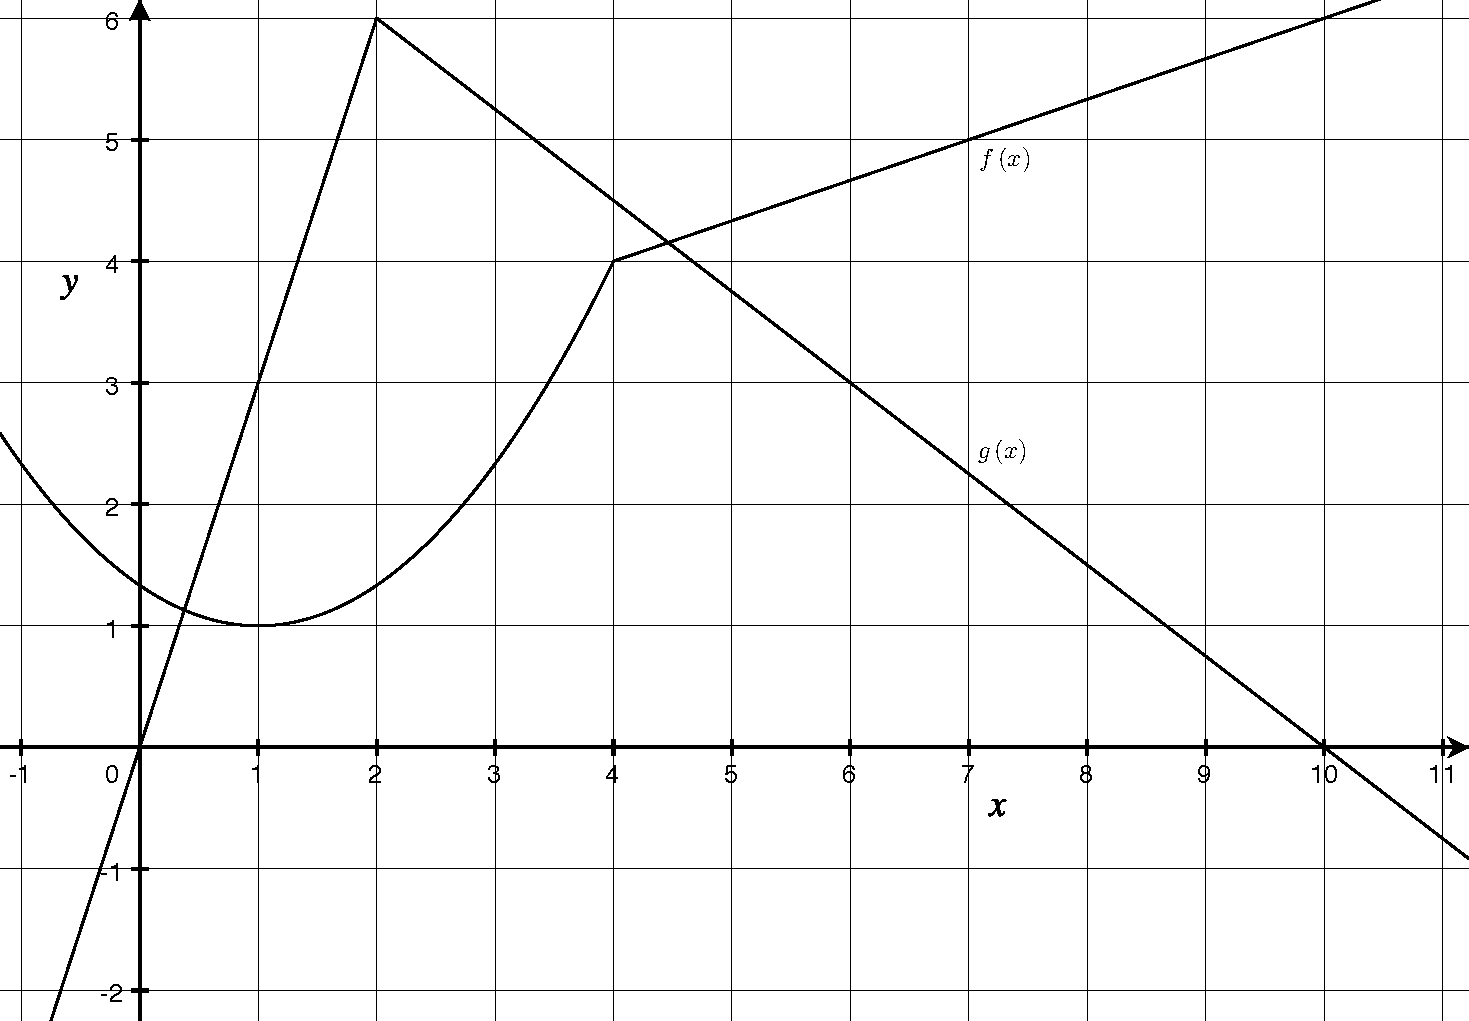
\includegraphics[width=4in]{./graphics/graph1501.pdf} 
   \caption{Both $f$ and $g$ are piecewise defined functions.}
   \label{fig:graph1501}
\end{figure}

And define $h\left( x \right) = \left( f  \circ g \right) \left( x \right) = f \left( g \left( x \right) \right)$. Using the chain rule, we have
\[
h'\left( x \right) = f' \left( g \left( x \right) \right) \cdot g' \left( x \right).
\]






\begin{questions}

\question Remember that we defined $h\left( x \right) = \left( f  \circ g \right) \left( x \right) = f \left( g \left( x \right) \right)$, and using the chain rule, we have $h'\left( x \right) = f' \left( g \left( x \right) \right) \cdot g' \left( x \right)$. From the information given, find each of the following. 

\begin{parts}

\part $\displaystyle h' \left( 1 \right)$.



\begin{solution}
Using the chain rule we have.
\[
h' \left( 1 \right) = f' \left( g \left( 1 \right) \right) \cdot g' \left( 1 \right) = f' \left( 3 \right) \cdot 3 = \frac{4}{3} \cdot 3
= 4
\]
\end{solution}


\part $\displaystyle h' \left( 0 \right)$



\begin{solution}
Using the chain rule we have.
\[
h' \left( 0 \right) = f' \left( g \left( 0 \right) \right) \cdot g' \left( 0 \right) = f' \left( 0 \right) \cdot 3 = -\frac{2}{3} \cdot 3
= -2
\]
\end{solution}


\part Does $\displaystyle h' \left( 2 \right)$ exist? If so, what does it equal?



\begin{solution}
Using the chain rule we see.
\[
h' \left( 2 \right) = f' \left( g \left( 2 \right) \right) \cdot g' \left( 2 \right)
\]
However, $g' \left( 2 \right)$ \emph{does not exists}, so the derivative is undefined at 2.
\end{solution}


\end{parts}

\question Now define $k\left( x \right) = \left( g  \circ f \right) \left( x \right) = g \left( f \left( x \right) \right)$. Using the chain rule, we have
\[
k'\left( x \right) = g' \left( f \left( x \right) \right) \cdot f' \left( x \right).
\]

From the information given, find each of the following.

\begin{parts}

\part $\displaystyle k' \left( 1 \right)$.



\begin{solution}
Using the chain rule we have.
\[
k' \left( 1 \right) = g' \left( f \left( 1 \right) \right) \cdot f' \left( 1 \right) = g' \left( 1 \right) \cdot 0 = 3 \cdot 0
= 0
\]
\end{solution}


\part $\displaystyle k' \left( 0 \right)$



\begin{solution}
Using the chain rule we have.
\[
k' \left( 0 \right) = g' \left( f \left( 0 \right) \right) \cdot f' \left( 0 \right) = g' \left( 4/3 \right) \cdot \left( -2/3 \right) = 3 \cdot \left( -2/3 \right)
= -2
\]
\end{solution}


\part Does $\displaystyle k' \left( 4 \right)$ exist? If so, what does it equal?



\begin{solution}
Using the chain rule we see.
\[
k' \left( 4 \right) = g' \left( f \left( 4 \right) \right) \cdot f' \left( 4 \right)
\]
However, $f' \left( 4 \right)$ \emph{does not exists}, so the derivative is undefined at 4.
\end{solution}


\end{parts}
\end{questions}

\subsection{Examples}
Find the indicated derivatives of each of the following.
\begin{questions}
\question $\qquad \displaystyle \frac{{\rm{d}}}{{\rm{d}}x}\left[ \left( x^2 - 2x + 3 \right)^5 \right] = $
\begin{solution}
This will be discussed in class.

Final answer:
\[
\frac{{\rm{d}}}{{\rm{d}}x}\left[ \left( x^2 - 2x + 3 \right)^5 \right] =  5 \left( x^2 - 2x + 3 \right)^4 \cdot \left( 2x^2 - 2 \right) 
\]
\end{solution}
\question $\qquad \displaystyle \frac{{\rm{d}}}{{\rm{d}}x}\left[ \left( \frac{x^2 + 4}{x^3-1} \right)^5 \right] = $
\begin{solution}
This will be discussed in class.

Final answer:
\[
\frac{{\rm{d}}}{{\rm{d}}x}\left[ \left( \frac{x^2 + 4}{x^3-1} \right)^5 \right] =  5\left( \frac{x^2 + 4}{x^3-1} \right)^4 \cdot \frac{\left(x^3-1\right) 2x - \left(x^2+4\right)3x^2}{\left(x^3-1\right)^2}
\]
\end{solution}

\question $\qquad \displaystyle \frac{{\rm{d}}}{{\rm{d}}x}\left[ \sin^2 x \right] = $
\begin{solution}
This will be discussed in class.

Final answer:
\[
\frac{{\rm{d}}}{{\rm{d}}x}\left[ \sin^2 x \right] =  2 \sin x \cdot \cos x
\]
\end{solution}


\question $\qquad \displaystyle \frac{{\rm{d}}}{{\rm{d}}x}\left[ \sqrt{\frac{1}{x+1}} \right] = $
\begin{solution}
This will be discussed in class.

Final answer:
\[
\frac{{\rm{d}}}{{\rm{d}}x}\left[ \sqrt{\frac{1}{x+1}} \right] = \frac{{\rm{d}}}{{\rm{d}}x}\left[ \left( x+1\right)^{-1/2} \right] =  -\frac{1}{2\left( x+1\right)\sqrt{x+1}}
\]
\end{solution}
\question $\qquad \displaystyle \frac{{\rm{d}}}{{\rm{d}}x}\left[ \sin^2 e^{x^2} \right] = $
\begin{solution}
This will be discussed in class.

Final answer:
\[
\frac{{\rm{d}}}{{\rm{d}}x}\left[ \sin^2 e^{x^2} \right] = 4x e^{x^2} \sin e^{x^2} \cos e^{x^2}= 2x e^{x^2} \sin \left( 2e^{x^2} \right)
\]


Here's the Mathematica code (Figure \ref{fig:mathematica15}, page \pageref{fig:mathematica15}) to do this problem. Learning to use a computer algebra system (CAS) such as Mathematica should be done well before you actually need it. Please take the time to play with a CAS system, even if it is just using a graphics calculator.
\end{solution}
\begin{figure}[htbp] %  figure placement: here, top, bottom, or page
   \centering
   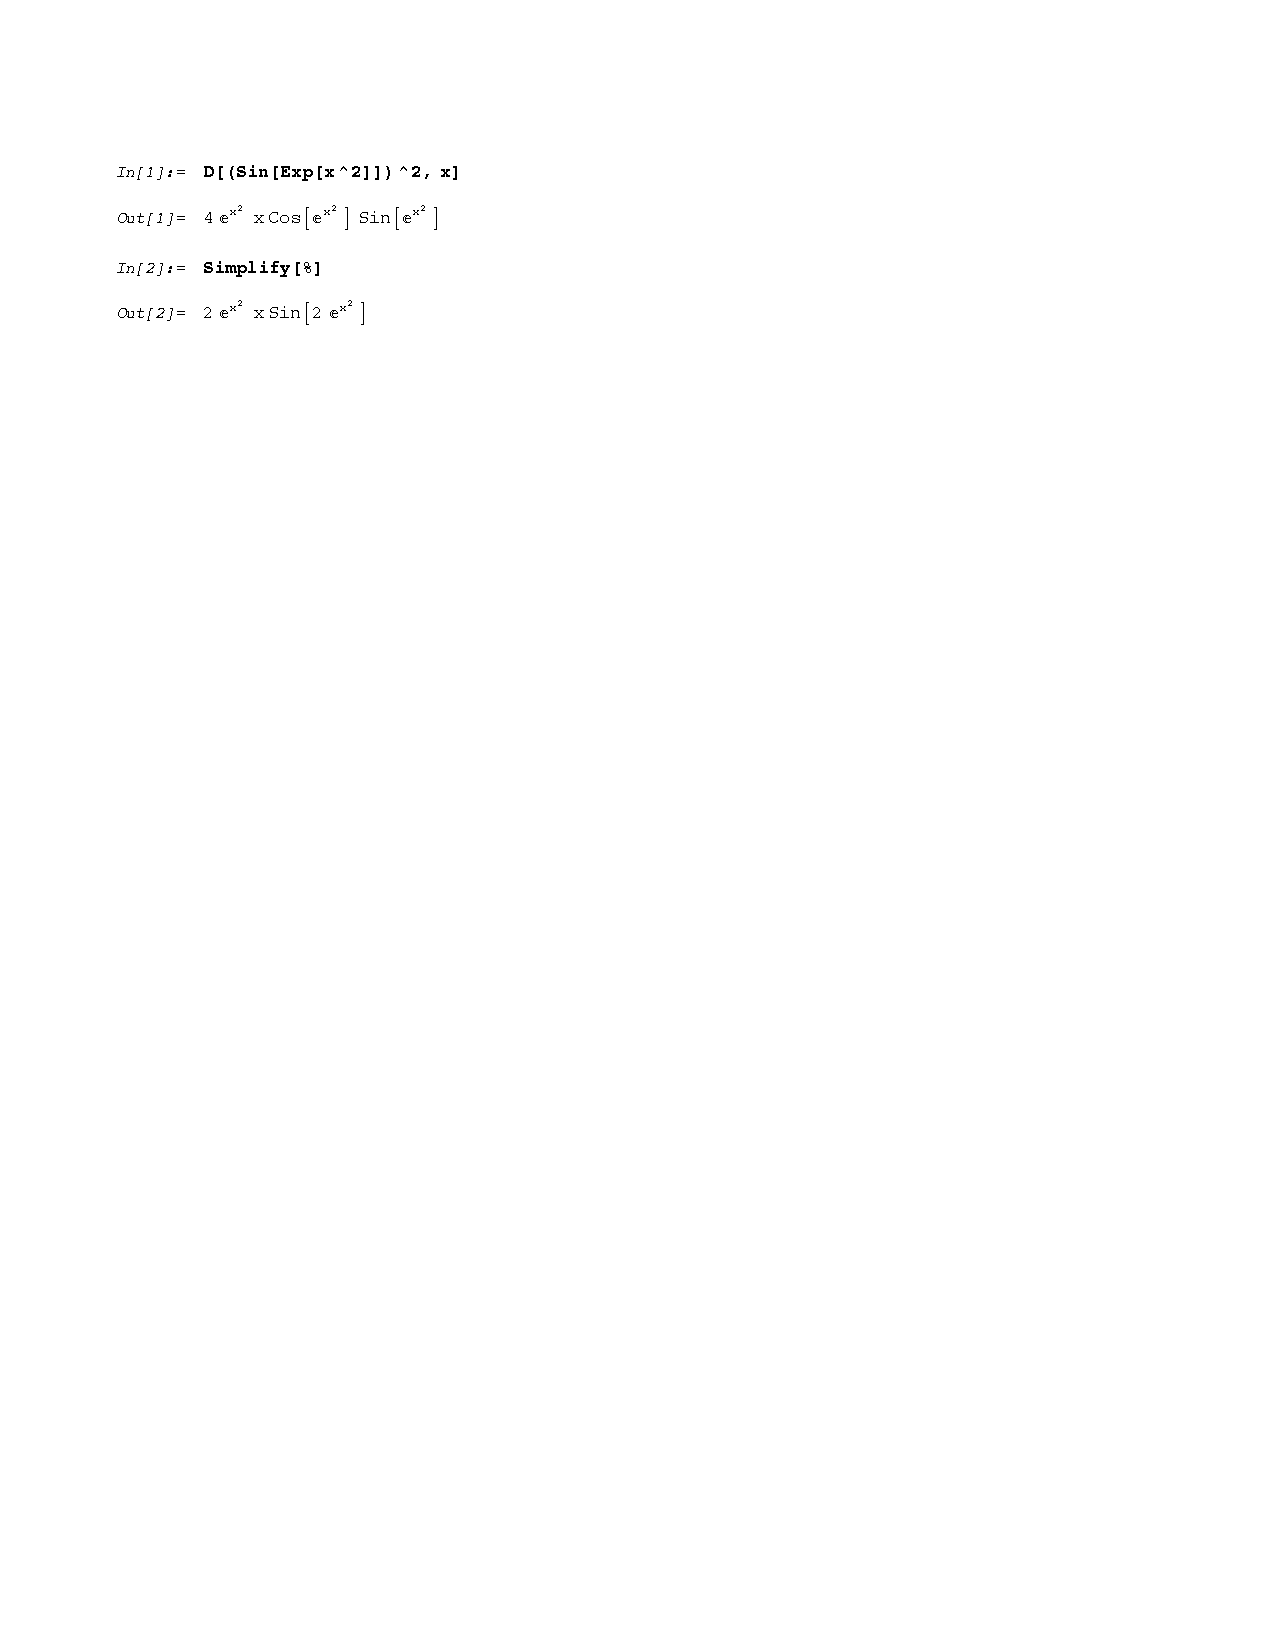
\includegraphics[width=3in]{./graphics/mathematica15.pdf} 
   \caption{Mathematica code,  program available in many student labs.}
   \label{fig:mathematica15}
\end{figure}


\question $\qquad \displaystyle \frac{{\rm{d}}}{{\rm{d}}x}\left[ \cos^3 \left(x^2 + 2x -3\right) \right] = $
\begin{solution}
This will be discussed in class.

Final answer:
\[
\frac{{\rm{d}}}{{\rm{d}}x}\left[ \cos^3 \left(x^2 + 2x -3\right) \right] =  -3 \cos^2 \left(x^2 + 2x -3\right) \cdot \sin \left(x^2 + 2x -3\right) \cdot  \left(2x + 2\right)
\]
\end{solution}





\question $\qquad \displaystyle \frac{{\rm{d}}}{{\rm{d}}x}\left[ \sqrt{5x^2 - 2x + 3} \right] = $
\begin{solution}
This will be discussed in class.

Final answer:
\[
\frac{{\rm{d}}}{{\rm{d}}x}\left[ \sqrt{5x^2 - 2x + 3} \right] =  \frac{10x - 2}{2 \sqrt{5x^2 - 2x + 3}}
\]

\end{solution}

\end{questions}







 
 



\subsection{Assignment}
You should read \S  3.7 and do the WebAssign assignment mth.121.03.07.

\vfill
\pagebreak
%*-*-*-*-*-*-*-*-*-*-*-*-*-*-*-*-*-*-*-*-*-*-*-*-*-*-*-*-*-*-*-*-*-*-*-*-*-*-*-*-*-*-*-*-*-*-*-*-*-*-*-*-*-*-*-*-*-*-*-*-*-*-*-*-*-*-*-*-*-*-*-*-*-*-*-*-*-*-*-*-*-*-*-*-
\begin{teacher}
\subsection{Assessments}
The following questions are related to the WebAssign assignments and may be used to assess students' ability. Please do not share any of these questions with students.
\begin{questions}	
\question 	%RogaCalcET2 3.7.006	WA-1723141

Calculate the following derivative if $y = \cos \left( 7x^3 \right)$.
\begin{solution}
Work
\end{solution}
\question 	%RogaCalcET2 3.7.029	WA-1723133

Calculate the following derivative.
\[
\frac{{\rm{d}}}{{\rm{d}}x} \left( 3 \sin \left(x^4\right) \right)
\]
\begin{solution}
Work
\end{solution}
\question 	%RogaCalcET2 3.7.030	WA-1723127


Calculate the following derivative.
\[
\frac{{\rm{d}}}{{\rm{d}}x} \left(  \sin^3 \left(2x\right) \right)
\]
\begin{solution}
Work
\end{solution}
\question 	%RogaCalcET2 3.7.031	WA-1755950

Use the Chain Rule to find the derivative.
\[
y = \sqrt{\left(6t\right)^2+9}
\]
\begin{solution}
Work
\end{solution}
\question 	%RogaCalcET2 3.7.032	WA-1723148

Calculate the following derivative.
\[
\frac{{\rm{d}}}{{\rm{d}}x} \left[ \left( x^2+5x+1\right)^{-5/2} \right]
\]
\begin{solution}
Work
\end{solution}
\question 	%RogaCalcET2 3.7.034	WA-1723142

Calculate the following derivative.
\[
\frac{{\rm{d}}}{{\rm{d}}x} \left[ \left( \sqrt{x+2} -1 \right)^{7/2} \right]
\]
\begin{solution}
Work
\end{solution}
\question 	%RogaCalcET2 3.7.035	WA-1723139

Calculate the following derivative.
\[
\frac{{\rm{d}}}{{\rm{d}}x} \left[ \left(\frac{x+6}{x-6}\right)^7 \right]
\]
\begin{solution}
Work
\end{solution}
\question 	%RogaCalcET2 3.7.036	WA-1755954

Use the chain rule to find the derivative.
\[
y = \cos^3 \left(2\theta\right)
\]
\begin{solution}
Work
\end{solution}
\question 	%RogaCalcET2 3.7.038	WA-1755945

Use the chain rule to find the derivative.
\[
y = \tan \left( 4 \theta^2 - 8 \theta \right)
\]
\begin{solution}
Work
\end{solution}
\question 	%RogaCalcET2 3.7.040	WA-1755955

Use the chain rule to find the derivative.
\[
y = e^{2x^{12}}
\]
\begin{solution}
Work
\end{solution}
\question 	%RogaCalcET2 3.7.041	WA-1755922

Use the chain rule to find the derivative.
\[
y = e^{1-6t^2}
\]
\begin{solution}
Work
\end{solution}
\question 	%RogaCalcET2 3.7.053	WA-1723122

Calculate the following derivative.
\[
\frac{{\rm{d}}}{{\rm{d}}x} \left[ \left( \cos \left(3x\right) + \sin \left( x^7\right)\right)^{1/2} \right]
\]
\begin{solution}
Work
\end{solution}
\question 	%RogaCalcET2 3.7.057	WA-1761516

Calculate the following derivative.
\[
\frac{{\rm{d}}}{{\rm{d}}x} \left[ \sqrt{\frac{3z+2}{3z-2}} \right]
\]
\begin{solution}
Work
\end{solution}
\question 	%RogaCalcET2 3.7.065	WA-1723130

Calculate the following derivative.
\[
\frac{{\rm{d}}}{{\rm{d}}x} \left[ \left( 2e^{5x} + 3e^{-2x}\right)^{6} \right]
\]
\begin{solution}
Work
\end{solution}
\question 	%RogaCalcET2 3.7.067	WA-1755953

Find the derivative using the appropriate rule or combination of rules.
\[
y = e^{\left( 5x^2+5x+4\right)^2}
\]
\begin{solution}
Work
\end{solution}
\end{questions}
\end{teacher}
\vfill
\pagebreak

%*-*-*-*-*-*-*-*-*-*-*-*-*-*-*-*-*-*-*-*-*-*-*-*-*-*-*-*-*-*-*-*-*-*-*-*-*-*-*-*-*-*-*-*-*-*-*-*-*-*-*-*-*-*-*-*-*-*-*-*-*-*-*-*-*-*-*-*-*-*-*-*-*-*-*-*-*-*-*-*-*-*-*-*-
\section{mth.121.03.08}
\subsection{Derivatives of Inverse Functions}


Assuming that $f\left(x\right)$ is differentiable and one-to-one with inverse $f^{-1}\left(x\right) = g \left( x \right)$. If $a$ belongs to the domain of $g\left(x\right)$, and $f'\left(g\left(a\right)\right) \neq 0$, then
\[
g'\left(a\right) = \frac{1}{f'\left(g\left(a\right)\right)}.
\]
Here's a visual\footnote{This will be labeled in class!} (Figure \ref{fig:graph1606}, page \pageref{fig:graph1606}) of what we are saying here.
\begin{figure}[htbp] %  figure placement: here, top, bottom, or page
   \centering
   \includegraphics[width=4in]{./graphics/graph1606.pdf} 
   \caption{Partial graph of $f$, $f^{-1}$, $y=x$, and two tangent lines.}
   \label{fig:graph1606}
\end{figure}



\textbf{Example:} Find the inverse of
\[
f\left( x \right) = \frac{1}{1+x},
\]
and then, using this inverse, compute
\[
\frac{{\rm{d}}}{{\rm{d}}x} \left[ f^{-1} \left( x \right) \right].
\]
Now verify that
\[
\frac{{\rm{d}}}{{\rm{d}}x} \left[ f^{-1} \left( x \right) \right] = \frac{1}{f'\left( f^{-1} \left( x \right) \right)}
\]

\begin{solution}
You should be able to show that
\[
f^{-1} \left( x \right) = \frac{1-x}{x}.
\]
And that
\[
\frac{{\rm{d}}}{{\rm{d}}x} \left[ f^{-1} \left( x \right) \right] = -\frac{1}{x^2}.
\]
And for the next step you'll need
\[
f'\left( x \right) = -\frac{1}{\left( 1 + x \right)^2}.
\]
And finally.
\begin{eqnarray*}
\frac{{\rm{d}}}{{\rm{d}}x} \left[ f^{-1} \left( x \right) \right] &=& \frac{1}{f'\left( f^{-1} \left( x \right) \right)}\\
-\frac{1}{x^2} &=& \frac{1}{f'\left( \displaystyle  \frac{1-x}{x} \right)}\\
&=& \frac{1}{ \displaystyle  -\frac{1}{ \left( 1 + \frac{1-x}{x} \right)^2}}\\
&=& - \left( 1 + \frac{1-x}{x} \right)^2\\
&=& -\frac{1}{x^2}
\end{eqnarray*}

\end{solution}

\subsubsection{Trigonometric Functions}

This is mostly a review of what was covered in MTH-120. I'm not suggesting that you need to know \emph{everything} that was covered in MTH-120, but you should be able to follow today's material without too much trouble if you learned the basics. Here's goes.
\begin{figure}[htbp] %  figure placement: here, top, bottom, or page
   \centering
   \includegraphics[width=4in]{./graphics/graph1601.pdf} 
   \caption{The three big trigonometric functions and their inverses, domain restrictions apply.}
   \label{fig:graph1601}
\end{figure}

The point here is that the trigonometric functions are not invertible unless we restrict their domains. I believe you should know sine, cosine and tangent well enough to construct a reasonable domain restriction to make these three functions \emph{one-to-one}. On the graph above you should be able to clearly identify all three functions and their inverses, the dashed-line $y=x$ is drawn on this graph as an aid.



Today we will derive the following derivatives.
\begin{enumerate}
\item Restrictions will be discussed later.
\[
\frac{{\rm{d}}}{{\rm{d}}x} \left( \arcsin x \right) = \frac{1}{\sqrt{1-x^2}}
\]
\item Restrictions will be discussed later.
\[
\frac{{\rm{d}}}{{\rm{d}}x} \left( \arccos x \right) = -\frac{1}{\sqrt{1-x^2}}
\]
\item Restrictions will be discussed later.
\[
\frac{{\rm{d}}}{{\rm{d}}x} \left( \arctan x \right) = \frac{1}{1+x^2}
\]
\end{enumerate}

I will not cover\footnote{Most books also covers cosecant, secant and cotangent, however, I don't require them for this course. If needed, just look them up, or derive them on the fly.} the derivatives of the other three trigonometric inverses, but here they are just in case you're interested:
\begin{enumerate}
\item
\[
\frac{{\rm{d}}}{{\rm{d}}x} \left( \csc^{-1} x \right) = -\frac{1}{\left|x\right|\sqrt{x^2-1}}
\]
\item
\[
\frac{{\rm{d}}}{{\rm{d}}x} \left( \sec^{-1} x \right) = \frac{1}{\left|x\right|\sqrt{x^2-1}}
\]
\item
\[
\frac{{\rm{d}}}{{\rm{d}}x} \left( \cot^{-1} x \right) = -\frac{1}{1+x^2}
\]
\end{enumerate}
\subsection{Finding the Derivatives of Inverse Trigonometric Functions}
\begin{figure}[htbp] %  figure placement: here, top, bottom, or page
   \centering
   \includegraphics[width=4in]{./graphics/graph1602.pdf} 
   \caption{The sine and its inverse, arcsine.}
   \label{fig:graph1602}
\end{figure}
Here's a graph (Figure \ref{fig:graph1602}, page \pageref{fig:graph1602}) of the sine function and its inverse. Carefully look at the graph and answer the following questions.
\begin{questions}
\question Label directly on the graph the sine function.

\begin{solution}
This will be \emph{quickly} discussed in class.
\end{solution}

\question What is the domain of this sine graph?

\begin{solution}
This will be \emph{quickly} discussed in class.
\end{solution}

\question What is the range of this sine graph?

\begin{solution}
This will be \emph{quickly} discussed in class.
\end{solution}

\question Label directly on the graph the arcsine function.

\begin{solution}
This will be \emph{quickly} discussed in class.
\end{solution}

\question What is the domain of this arcsine graph?

\begin{solution}
This will be \emph{quickly} discussed in class.
\end{solution}

\question What is the range of this arcsine graph?

\begin{solution}
This will be \emph{quickly} discussed in class.
\end{solution}

\question To find the derivative of $y = \arcsin x$, we note that $\sin y = x$ and differentiate.
\begin{solution}
This will be discussed in class.
\end{solution}



\end{questions}



\begin{figure}[htbp] %  figure placement: here, top, bottom, or page
   \centering
   \includegraphics[width=4in]{./graphics/graph1603.pdf} 
   \caption{The cosine and its inverse, arccosine.}
   \label{fig:graph1603}
\end{figure}
Here's a graph of the cosine (Figure \ref{fig:graph1603}, page \pageref{fig:graph1603}) function and its inverse. Carefully look at the graph and answer the following questions.
\begin{questions}
\question Label directly on the graph the cosine function.

\begin{solution}
This will be discussed in class.
\end{solution}

\question What is the domain of this cosine graph?

\begin{solution}
This will be \emph{quickly} discussed in class.
\end{solution}

\question What is the range of this cosine graph?

\begin{solution}
This will be \emph{quickly} discussed in class.
\end{solution}

\question Label directly on the graph the arccosine function.

\begin{solution}
This will be \emph{quickly} discussed in class.
\end{solution}

\question What is the domain of this arccosine graph?
\begin{solution}
This will be \emph{quickly} discussed in class.
\end{solution}


\question What is the range of this arccosine graph?

\begin{solution}
This will be \emph{quickly} discussed in class.
\end{solution}

\question To find the derivative of $y = \arccos x$, we note that $\cos y = x$ and differentiate. We'll do this in class.

\begin{solution}
This will be discussed in class.
\end{solution}

\end{questions}



\begin{figure}[htbp] %  figure placement: here, top, bottom, or page
   \centering
   \includegraphics[width=4in]{./graphics/graph1604.pdf} 
   \caption{The tangent and its inverse, arctangent.}
   \label{fig:graph1604}
\end{figure}
Here's a graph  (Figure \ref{fig:graph1604}, page \pageref{fig:graph1604}) of the tangent function and its inverse. Carefully look at the graph and answer the following questions.
\begin{questions}
\question Label directly on the graph the tangent function.

\begin{solution}
This will be \emph{quickly} discussed in class.
\end{solution}

\question What is the domain of this tangent graph?

\begin{solution}
This will be \emph{quickly} discussed in class.
\end{solution}

\question What is the range of this tangent graph?
\begin{solution}
This will be \emph{quickly} discussed in class.
\end{solution}

\question Label directly on the graph the arctangent function.

\begin{solution}
This will be \emph{quickly} discussed in class.
\end{solution}

\question What is the domain of this arctangent graph?

\begin{solution}
This will be \emph{quickly} discussed in class.
\end{solution}

\question What is the range of this arctangent graph?

\begin{solution}
This will be \emph{quickly} discussed in class.
\end{solution}

\question To find the derivative of $y = \arctan x$, we note that $\tan y = x$ and differentiate. We'll do this in class.
\begin{solution}
This will be discussed in class.
\end{solution}
\end{questions}






 
 
\subsection{Examples}

\begin{questions}

\question Find the derivative.
\[
y = \sin^{-1} x^2
\]
\begin{solution}
This will be discussed in class.

Final answer:
\[
y' =  \frac{2x}{\sqrt{1-x^4}}
\]
\end{solution}


\question Find the derivative.
\[
 y = e^{\cos^{-1} \left(1-x^2\right)}
 \]
\begin{solution}
This will be discussed in class.

Final answer:
\[
y'  =  \frac{2xe^{\cos^{-1} \left(1-x^2\right)}}{\sqrt{1-\left(1-x^2\right)^2}} 
\]
\end{solution}


\question Find the derivative.
\[
 y = x\tan^{-1} x
 \]
\begin{solution}
This will be discussed in class.

Final answer:
\[
 y' = \tan^{-1} x + \frac{x}{1+x^2}
 \]
\end{solution}


\question Find the derivative.
\[
 y = \sin^{-1} \frac{x}{1+x}
\]
\begin{solution}
This will be discussed in class.

Final answer:
\[
y' =  \frac{1}{\left(1+x\right)^2\sqrt{1-\left(\frac{x}{1+x}\right)^2}}
\]
\end{solution}


\question Find the derivative.
\[
y = \cos \left[ \arcsin \left( x + 1 \right) \right]
\]
\begin{solution}
This will be discussed in class.

Final answer:
\[
y' = -\frac{1+x}{\sqrt{1-(1+x)^2}}
\]
\end{solution}


\question Given the following graph\footnote{Scale is not preserved.} (Figure \ref{fig:graph1605}, page \pageref{fig:graph1605}),
\begin{figure}[htbp] %  figure placement: here, top, bottom, or page
   \centering
   \includegraphics[width=4in]{./graphics/graph1605.pdf} 
   \caption{$f \left( x \right) = x \arcsin \left( 1 - x^2 \right)$}
   \label{fig:graph1605}
\end{figure}

answer the following questions about $f \left( x \right)$:
\begin{parts}


\part domain (interval notation);
\begin{solution}
First, you should know that the domain of the arcsine function is $\left[ -1, \ 1 \right]$, so we need to solve
\begin{eqnarray*}
-1 \leq  1 -x^2 \leq  1\\
-2 \leq  - x^2\leq  0\\
0 \leq x^2 \leq 2\\
-\sqrt{2} \leq  x \leq  \sqrt{2}
\end{eqnarray*}
So the domain is
\[
\left[-\sqrt{2}, \ \sqrt{2}\right] \approx \left[-1.4142, \ 1.4142 \right] .
\]
\end{solution}


\part range (interval notation);
\begin{solution}
Using the result from part (a). Evaluating the left endpoint:
\begin{eqnarray*}
f \left( -\sqrt{2} \right) &=& \left( -\sqrt{2} \right) \arcsin \left[ 1 - \left(-\sqrt{2}\right)^2 \right]\\
&=& \left( -\sqrt{2} \right) \arcsin \left[ 1 - 2 \right]\\
&=& \left( -\sqrt{2} \right) \arcsin \left[ -1 \right]\\
&=& \left( -\sqrt{2} \right) \left(-\frac{\pi}{2}\right)\\
&=& \frac{\pi\sqrt{2}}{2}
\end{eqnarray*}
and evaluating the right endpoint:
\begin{eqnarray*}
f \left( \sqrt{2} \right) &=& \left( \sqrt{2} \right) \arcsin \left[ 1 - \left(\sqrt{2}\right)^2 \right]\\
&=& \left( \sqrt{2} \right) \arcsin \left[ 1 - 2 \right]\\
&=& \left( \sqrt{2} \right) \arcsin \left[ -1 \right]\\
&=& \left( \sqrt{2} \right) \left(-\frac{\pi}{2} \right)\\
&=& -\frac{\pi\sqrt{2}}{2}
\end{eqnarray*}
Finally the range is:
\[
 \left[ -\frac{\pi\sqrt{2}}{2}, \ \frac{\pi\sqrt{2}}{2} \right] \approx \left[-2.2214, \ 2.2214 \right].
\]

\end{solution}



\end{parts}


\end{questions}


















 









































\subsection{Assignment}
You should read \S  3.8 and do the WebAssign assignment mth.121.03.08.
\vfill
\pagebreak
%*-*-*-*-*-*-*-*-*-*-*-*-*-*-*-*-*-*-*-*-*-*-*-*-*-*-*-*-*-*-*-*-*-*-*-*-*-*-*-*-*-*-*-*-*-*-*-*-*-*-*-*-*-*-*-*-*-*-*-*-*-*-*-*-*-*-*-*-*-*-*-*-*-*-*-*-*-*-*-*-*-*-*-*-
\begin{teacher}
\subsection{Assessments}
The following questions are related to the WebAssign assignments and may be used to assess students' ability. Please do not share any of these questions with students.
\begin{questions}		
\question 	%RogaCalcET2 3.8.001	WA-1723559
 
Find the inverse $g\left(x\right)$ of $f\left(x\right) = \sqrt{x^8 + 10}$ with domain $x \geq 0$. And calculate $g'\left(x\right)$.
\begin{solution}
Work
\end{solution}

\question 	%RogaCalcET2 3.8.004	WA-1723557

Use Theorem 1 to calculate $g'\left(x\right)$, where $g\left(x\right)$ is the inverse of $f\left(x\right) = \sqrt{6 - 4x}$.
\begin{solution}
Work
\end{solution}

\question 	%RogaCalcET2 3.8.009	WA-1739131

Let $g\left(x\right)$ be the inverse of $f\left(x\right) = x^3 + 3x + 6$.
\begin{parts}
\part Calculate $g\left( 20 \right)$ [without finding a formula for $g\left(x\right)$].
\begin{solution}
Work
\end{solution}
\part Calculate $g'\left( 20 \right)$.
\begin{solution}
Work
\end{solution}
\end{parts}

\question 	%RogaCalcET2 3.8.018	WA-1738337

Let $f\left(x\right) = \displaystyle \frac{1}{2+2x}$ and $g\left(x\right) = \displaystyle \frac{1-2x}{2x}$. Compute the following.
\begin{parts}
\part $f\left( g \left( x\right) \right) =$
\begin{solution}
Work
\end{solution}
\part $g\left( f \left( x\right) \right) =$
\begin{solution}
Work
\end{solution}
\part $g' \left(x \right) =$
\begin{solution}
Work
\end{solution}
\part  $\displaystyle \frac{1}{f'\left( g \left( x\right) \right)} =$
\begin{solution}
Work
\end{solution}
\end{parts}

\question 	%RogaCalcET2 3.8.019	WA-1761143

Compute the derivative of $y = \arcsin x$ at $x = 4/7$ without using a calculator.
\begin{solution}
Work
\end{solution}
\question 	%RogaCalcET2 3.8.024	WA-1761067

Find the derivative of $y = \arctan \left(x/3\right)$.
\begin{solution}
Work
\end{solution}

\question 	%RogaCalcET2 3.8.025	WA-1723815

Find the derivative of $y = \arccos \left( 9x^5\right)$.
\begin{solution}
Work
\end{solution}

\question 	%RogaCalcET2 3.8.031	WA-1723499

Find the derivative of $y = \sqrt{6 - x^2} + \arcsin \left( 5x \right)$.
\begin{solution}
Work
\end{solution}

\question 	%RogaCalcET2 3.8.032	WA-1761146

Find the derivative of $y = \arctan \displaystyle \frac{5+t}{5-t}$.
\begin{solution}
Work
\end{solution}

\question 	%RogaCalcET2 3.8.033	WA-1738366

Find the derivative of $y = \left(\arctan x\right)^3$.
\begin{solution}
Work
\end{solution}

\end{questions}
\end{teacher}
\vfill
\pagebreak

%*-*-*-*-*-*-*-*-*-*-*-*-*-*-*-*-*-*-*-*-*-*-*-*-*-*-*-*-*-*-*-*-*-*-*-*-*-*-*-*-*-*-*-*-*-*-*-*-*-*-*-*-*-*-*-*-*-*-*-*-*-*-*-*-*-*-*-*-*-*-*-*-*-*-*-*-*-*-*-*-*-*-*-*-
\section{mth.121.03.09}
\subsection{Logarithmic Functions}

Much of what we do in MTH-121 depends on material covered in MTH-119 and MTH-120. From MTH-119 you should recall that the general logarithmic function is of the form
\[
\log_a x = y
\]
where $a$ is a positive constant, $a \neq 1$, and $x > 0$.



In MTH-119 you also learned how to graph and solve logarithmic equations. The basis for much of your work (either graphing or solving equations) was the following fact:
\[
\log_a x = y \qquad \Leftrightarrow \qquad x = a^y.
\]
So, I hope it is clear that the inverse of the logarithm (base $a$) is the exponential (base $a$), and \emph{vise versa}. A simple graph illustrates this fact nicely.
\begin{figure}[htbp] %  figure placement: here, top, bottom, or page
   \centering
   \includegraphics[width=3in]{./graphics/graph1701.pdf} 
   \caption{$y=e^x$ in blue; $y = x$ red dash; and $y=\ln x$ in green.}
   \label{fig:graph1701}
\end{figure}

\subsubsection{Derivatives of Natural Logarithmic Functions}

We know from a prior worksheet that
\[
\frac{{\rm{d}}}{{\rm{d}}x} \left( e^x \right) = e^x.
\]
Let's use this fact to find the derivative of
\[
y = \ln x.
\]
Knowing small facts about $e^x$ will allow us to find the derivative of $\ln x$. Here goes.
\begin{eqnarray*}
y &=& \ln x\\
e^y &=& x\\
\frac{{\rm{d}}}{{\rm{d}}x} \left( e^y \right) &=& \frac{{\rm{d}}}{{\rm{d}}x} \left(  x \right)\\
e^y \frac{{\rm{d}}y}{{\rm{d}}x} &=& 1\\
\frac{{\rm{d}}y}{{\rm{d}}x} &=& \frac{1}{e^y}.
\end{eqnarray*}
This is not the usual way to write the derivative of $\ln x$, so we need to rewrite $e^y$ in terms of $x$. Again, using what we already know about logarithms.
\begin{eqnarray*}
y &=& \ln x\\
e^y &=& x.
\end{eqnarray*}
Finally, we have:
\[
y = \ln x \qquad \Rightarrow \qquad y' = \frac{1}{x}.
\]
\subsubsection{Other Bases?}

Well you are bound to see other bases, for example, suppose you are asked to find the derivative of an exponential function whose base is not $e$? A general example, find the derivative of
\[
y = a^x, \quad a > 0.
\]
I personally don't believe it's worth memorizing, but you should be able to follow these steps.
\begin{eqnarray*}
y &=& a^x\\
\ln y &=& x \ln a\\
\frac{1}{y} y' &=& \ln a\\
y' &=& y \ln a\\
y' &=& a^x \ln a
\end{eqnarray*}
So now we have another result.
\[
y = a^x, \quad a > 0 \ \mbox{and} \ a \neq 1 \qquad \Rightarrow \qquad y' = a^x \ln a
\]



What about logarithms where the base is not $e$. I strongly suggest that you use the base change formula that you learned in MTH-119.\footnote{I'll review this in class.}
\[
y = \log_a x \qquad \Rightarrow \qquad y = \frac{\ln x}{\ln a}
\]
So if you're asked to find the derivative of
\[
y = \log_3 x,
\]
I suggest that you rewrite this as
\[
y = \frac{\ln x }{\ln 3},
\]
and then differentiate.
\[
y = \log_3 x \qquad \Rightarrow \qquad y' = \frac{1}{x\ln3}
\]

\subsection{Examples}

\begin{questions}
\question Differentiate.
\[
y = \frac{1}{1 + \ln x}
\]
\begin{solution}
This will be discussed in class. Final answer:
\[
y' = -\frac{1}{x\left( 1 + \ln x \right)^2}
\]
\end{solution}


\question Find the limit.
\[
\mathop {\lim }\limits_{x \to \infty} \left[ \ln \left( 2 + x \right) - \ln \left( 1 + x \right) \right]
\]
\begin{solution}
This will be discussed in class. Final answer:
\[
0
\]
\end{solution}


\question Find the domain and range of $y = \ln \left( e^x - 2 \right)$.
\begin{solution}
This will be discussed in class. Final answer:
The domain is
\[
\left( \ln 2 , \ \infty \right)
\]
and the range is
\[
\mathbb{R}.
\]
\end{solution}


\question Find $y'$, if $y = \ln \left( x^4 \sin^2 x \right)$.
\begin{solution}
This will be discussed in class.

Final answer:
\[
y ' = \frac{4}{x} + 2 \cot x
\]
\end{solution}


\question Find the limit.
\[
\mathop {\lim }\limits_{x \to 3^+} \log_{10} \left( x^2 -5x+6\right)
\]
\begin{solution}
This will be discussed in class.

Final answer:
\[
-\infty
\]
\end{solution}


\question Given $y = \sqrt{x} e^{x^2} \left(x^2 + 1 \right)^{10}$, answer each of the following questions.\footnote{An example of logarithmic differentiation.}
\begin{parts}
\part Take the natural log of both sides and expand the right side completely.
\begin{solution}
This will be discussed in class.

Final answer:
\[
\ln y = \frac{1}{2} \ln x +  x^2 + 10 \ln \left(x^2 + 1 \right)
\]
\end{solution}
\part Differentiate both sides.
\begin{solution}
This will be discussed in class. 

Final answer:
\[
\frac{1}{y} y' = \frac{1}{2x} +  2x + \frac{20x}{x^2 + 1 }
\]
\end{solution}
\part Find $y'$.
\begin{solution}
This will be discussed in class. 

Final answer:
\[
 y' = \left(\sqrt{x} e^{x^2} \left(x^2 + 1 \right)^{10} \right)\left(\frac{1}{2x} +  2x + \frac{20x}{x^2 + 1 }\right)
\]
\end{solution}
\end{parts}

\question Given
\[
f \left( x \right) = \frac{1+e^x}{1-e^x},
\]
answer each of the following questions.









\begin{parts}
\part Find the domain of $f \left( x \right)$.
\begin{solution}
This will be discussed in class. Final answer:
\[
\mathbb{R}, \ x \neq 0
\]
\end{solution}


\part Find the range of $f \left( x \right)$.
\begin{solution}
This will be discussed in class. 

Final answer:
\[
\left( -\infty, \ -1 \right) \cup \left( 1, \ \infty \right)
\]
\end{solution}


\part Find $f^{-1} \left( x \right)$ and indicate its domain and range.
\begin{solution}
This will be discussed in class.

Final answers: The inverse is:
\[
f^{-1} \left( x \right) = \ln \frac{x-1}{x+1}.
\]
The domain is:
\[
\left( -\infty, \ -1 \right) \cup \left( 1, \ \infty \right)
\]

The range is:
\[
\mathbb{R}, \ x \neq 0
\]
\end{solution}


\part Graph $f^{-1} \left( x \right)$ and $f \left( x \right)$ on the same axis.
\begin{solution}
This will be discussed in class. Final answer:
 strongly encourage everyone to use technology to construct graphs (Figure \ref{fig:graph1702}, page \pageref{fig:graph1702}). For Mac OS X users I suggest Grapher (free); for Windows users I suggest WinPlot (free); and for Linux/UNIX users I suggest GNUPlot (free). A good web-based application is Wolfram Alpha.
\end{solution}
\begin{figure}[htbp] %  figure placement: here, top, bottom, or page
   \centering
   \includegraphics[width=4in]{./graphics/graph1702.pdf} 
   \caption{$f\left( x \right)$ in blue; $y = x$ red dash; and $f^{-1} \left( x \right)$ in green.}
 \label{fig:graph1702}
\end{figure}

\end{parts}

\question Find $y'$.
\[
x^y = y^x
\]
\begin{solution}
This will be discussed in class. 

Final answer:
\[
y' = \frac{\ln y - y/x}{ \ln x - x/y} = \frac{y^2 - xy \ \ln y}{x^2 - xy \ \ln x}
\]
\end{solution}


\end{questions}


\subsection{Assignment}
You should read \S  3.9 and do the WebAssign assignment math.121.03.09.

\vfill
\pagebreak





\subsection{Hyperbolic Functions [Optional Material]}

It's endless! No, but you'll see that many schools cover a lot of material in their Calculus classes, but I would prefer to cover fundamentals that will allow you to extend your knowledge without being overwhelmed with memorizing a lot of disconnected materials. So, please take a look at this \emph{optional} material to see that knowing a little can in fact be used as a basis for knowing a lot. Just don't try to memorize what follows, but you should nonetheless be able to do this on your own. No, you won't be tested on this.


Well, I can't say, ``once again!'' That is, the hyperbolic functions were not covered in MTH-119 or MTH-120, so we must begin afresh. So let's start with hyperbolic sine, abbreviated sinh, and hyperbolic cosine, abbreviated cosh.\footnote{The graph of the hyperbolic cosine is called a \emph{catenary}, the shape of a hanging cable.} They are defined as follows:
\[
\sinh x = \frac{e^x-e^{-x}}{2} \qquad \mbox{and} \qquad
\cosh x = \frac{e^x+e^{-x}}{2}.
\]
Their graphs follow:
\begin{figure}[htbp] %  figure placement: here, top, bottom, or page
   \centering
   \includegraphics[width=2.6in]{./graphics/graph1703.pdf} \includegraphics[width=2.6in]{./graphics/graph1704.pdf} 
   \caption{$y=\sinh x$ (left) and $y=\cosh x$ .}
   \label{fig:graph170304}
\end{figure}

The dashed red lines are not part of the graph, but I want to emphasize that these two functions are just simple combinations of $e^x$ and $e^{-x}$. We'll discuss, in class, the dashed red lines on the above two graphs.

\subsubsection{Some  Questions? [Optional Material]}
\begin{questions}
\question What is the domain of the hyperbolic sine?
\begin{solution}
Answer: $\mathbb{R}$
\end{solution}


\question What is the range of the hyperbolic sine?

\begin{solution}
Answer: $\mathbb{R}$
\end{solution}

\question Is the hyperbolic sine \emph{even}, \emph{odd}, or \emph{neither}?

\begin{solution}
Answer: \emph{odd}
\end{solution}

\question What is the domain of the hyperbolic cosine?

\begin{solution}
Answer: $\mathbb{R}$
\end{solution}

\question What is the range of the hyperbolic cosine?

\begin{solution}
Answer: $\left[ 1, \ \infty \right)$
\end{solution}

\question Is the hyperbolic cosine \emph{even}, \emph{odd}, or \emph{neither}?

\begin{solution}
Answer:  \emph{even}
\end{solution}

\question Show that
\[
\frac{{\rm{d}}}{{\rm{d}}x} \left( \cosh x \right) = \sinh x.
\]

\begin{solution}
Use the definitions!
\end{solution}


\question Show that
\[
\frac{{\rm{d}}}{{\rm{d}}x} \left( \cosh x \right) = \sinh x.
\]

\begin{solution}
Use the definitions!
\end{solution}


\question Show that
\[
\cosh^2 t - \sinh^2 t = 1.
\]

\begin{solution}
Use the definitions!
\end{solution}

\question If we define hyperbolic tangent as:
\[
\tanh x = \frac{\sinh x}{\cosh x},
\]
what is hyperbolic tangent in terms of $e^x$ and $e^{-x}$?


\begin{solution}
Use the definitions!
\end{solution}


\end{questions}




By the way, many Calculus textbooks have interesting pictures\footnote{The parametric variable, $t$, when dealing with the trigonometric functions, represents the angle. Interestingly enough, the $t$ is also related to the area of the sector of the unit circle; likewise, the same is true for the hyperbolic functions, but this time the area is not a sector, but the bounded region.} that relates the point,
\[
P\left( \cosh t, \ \sinh t \right) = \left( x, \ y \right),
\]
on a hyperbola to the origin $O\left( 0, \  0 \right)$ using the identity derived in the problem set above, that is $\cosh^2 t- \sinh^2 t = 1$ or $x^2 - y^2 =1$. Here's the graph of $x^2 - y^2 =1$, which is a hyperbola.\footnote{The circular functions relate the point $P\left( \cos t, \ \sin t \right) = \left( x, \ y \right)$ on a unit circle, $x^2+y^2=1$ to the origin $O\left( 0, \  0 \right)$.
}
\begin{figure}[htbp] %  figure placement: here, top, bottom, or page
   \centering
   \includegraphics[width=3in]{./graphics/graph1705.pdf} 
   \caption{Graph of $x^2 - y^2 =1$, which is a hyperbola.}
   \label{fig:graph1705}
\end{figure}



Hence, the reason why they're called hyperbolic, just as the trigonometric functions are often called circular. That is, the point $P\left( \cos t, \ \sin t \right) = \left( x, \ y \right)$ on a circle is related to the origin $O\left( 0, \  0 \right)$ using the identity $\cos^2 t + \sin^2 t = 1$ or $x^2 + y^2 =1$.



\textbf{Example:} Pick the point $\left( \sqrt{2}, \ 1 \right)$ on the hyperbola, $x^2-y^2=1$, and determine the exact value of $t$.\footnote{Again, the point $P\left( \cosh t, \ \sinh t \right) = \left( x, \ y \right)$ is on $x^2-y^2=1$.}


\begin{solution}
Let's find $t$ first.
\begin{eqnarray*}
\sinh t &=& 1\\
\frac{e^t - e^{-t}}{2} &=& 1\\
e^t - e^{-t} &=& 2 \qquad \mbox{multiply both sides by $e^t$}\\
e^{2t} - 1 &=& 2e^t \qquad \mbox{solve for zero}\\
e^{2t} - 2e^t - 1 &=& 0 \qquad \mbox{let $u=e^t$ and note that $u>0$}\\
u^2 - 2u - 1 &=& 0 \qquad \mbox{solve for $u$ using the quadratic formula}\\
u &=& 1 + \sqrt{2} \qquad \mbox{now solve for $t$, where $t= \ln u$.}\\
t &=& \ln \left( 1 + \sqrt{2} \right)
\end{eqnarray*}



Now, using this value of $t$, verify $\cosh t = \sqrt{2}$.
\begin{eqnarray*}
\cosh t &=& \sqrt{2}\\
\frac{e^t+e^{-t}}{2} &=& \sqrt{2}\\
\frac{e^{\ln \left( 1 + \sqrt{2} \right)}+e^{-\ln \left( 1 + \sqrt{2} \right)}}{2} &=& \sqrt{2}\\
\frac{\left( 1 + \sqrt{2} \right)+ \left( 1 + \sqrt{2} \right)^{-1}}{2} &=& \sqrt{2}\\
\frac{\left( 1 + \sqrt{2} \right)+ \left( \sqrt{2}-1 \right)}{2} &=& \sqrt{2}\\
\frac{2\sqrt{2}}{2} &=& \sqrt{2}\\
\sqrt{2} &=& \sqrt{2}\\
\end{eqnarray*}
So it should be clear why the term hyperbolic is used, and the reason that we see $sine$ $cosine$ and $tangent$ in these hyperbolic functions is mainly due to the fact that the identities they generate is reminiscent of the trigonometric identities.
\end{solution}

\subsubsection{Inverses [Optional Material]}

From what we know about inverses, it is clear that the hyperbolic sine is invertible, but the hyperbolic cosine is not. However, just like the trigonometric functions, we are going to restrict the domain of the hyperbolic cosine to make it a one-to-one function. For sake of argument, let's restrict the domain of the hyperbolic cosine to $x \geq 0$.



\textbf{Example:}  Try finding $\sinh^{-1} x$.

\begin{solution}
\begin{eqnarray*}
\sinh x &=& y\\
\sinh y &=& x\\
\frac{e^y - e^{-y}}{2} &=& x\\
e^y - e^{-y} &=& 2x \qquad \mbox{multiply both sides by $e^y$}\\
e^{2y} - 1 &=& 2xe^y \qquad \mbox{solve for zero}\\
e^{2y} - 2xe^y - 1 &=& 0 \qquad \mbox{let $u = e^y$}\\
u^{2} - 2xu - 1 &=& 0 \\
u &=& \frac{2x \pm \sqrt{4x^2 + 4}}{2} \qquad \mbox{quadratic formula}\\
e^y &=& x + \sqrt{x^2 + 1} \qquad \mbox{note the $\pm$ is now $+$}\\
y &=& \ln\left(x + \sqrt{x^2 + 1}\right) 
\end{eqnarray*}



\textbf{Side Note:} Why only the $+$ is used from the expression $x \pm \sqrt{x^2 + 1}$, because we know that $e^y > 0$, hence $x \pm \sqrt{x^2 + 1} > 0$, and since $x < \sqrt{x^2 + 1}$ for all $x$ we must exclude $x - \sqrt{x^2 + 1} < 0$. 

\end{solution}

\subsubsection{What You May Need to Know? [Optional Material]}

For this class, you do not need to know the hyperbolic functions, but some of you will enter fields that will use these functions. Just be aware that lots of named functions exists, and do look them up when needed. Have a good reference source, web-based or an actual textbook, whatever \emph{floats your boat}!

Certainly, after reading this optional section, you should be able to recall the definitions for the hyperbolic sine and cosine, and then follow what was presented in this section so far.
\begin{enumerate}
\item $\displaystyle \frac{{\rm{d}}}{{\rm{d}}x} \left( \sinh x \right) = \cosh x$
\item $\displaystyle \frac{{\rm{d}}}{{\rm{d}}x} \left( \cosh x \right) = \sinh x$
\item $\displaystyle \frac{{\rm{d}}}{{\rm{d}}x} \left( \mbox{tanh} \ x \right) = \mbox{sech}^2 \ x$
\item $\displaystyle \frac{{\rm{d}}}{{\rm{d}}x} \left( \mbox{csch} \ x \right) = -\mbox{csch} \ x \ \mbox{coth} \ x$
\item $\displaystyle \frac{{\rm{d}}}{{\rm{d}}x} \left( \mbox{sech} \ x \right) = -\mbox{sech} \ x \ \mbox{tanh} \ x$
\item $\displaystyle \frac{{\rm{d}}}{{\rm{d}}x} \left( \mbox{coth} \ x \right) = -\mbox{csch}^2 \ x$
\item $\displaystyle \sinh^{-1} x = \ln \left( x + \sqrt{x^2 + 1}\right), \quad x \in \mathbb{R}$
\item $\displaystyle \cosh^{-1} x = \ln \left( x + \sqrt{x^2 - 1}\right), \quad x \in \left[1, \ \infty \right)$
\item $\displaystyle \mbox{tanh}^{-1} x = \frac{1}{2} \ln \left( \frac{1+x}{1-x} \right), \quad x \in \left(-1, \ 1 \right)$
\item $\displaystyle \frac{{\rm{d}}}{{\rm{d}}x} \left( \sinh^{-1} x \right) = \frac{1}{\sqrt{1+x^2}}$
\item $\displaystyle \frac{{\rm{d}}}{{\rm{d}}x} \left( \cosh^{-1} x \right) = \frac{1}{\sqrt{x^2-1}}$
\item $\displaystyle \frac{{\rm{d}}}{{\rm{d}}x} \left( \mbox{tanh}^{-1} x \right) = \frac{1}{1-x^2}$
\item $\displaystyle \frac{{\rm{d}}}{{\rm{d}}x} \left( \mbox{csch}^{-1} x \right) = -\frac{1}{\left|x\right|\sqrt{1+x^2}}$
\item $\displaystyle \frac{{\rm{d}}}{{\rm{d}}x} \left( \mbox{sech}^{-1} x \right) = -\frac{1}{x\sqrt{1-x^2}}$
\item $\displaystyle \frac{{\rm{d}}}{{\rm{d}}x} \left( \mbox{coth}^{-1} x \right) = \frac{1}{1-x^2}$
\end{enumerate}
Believe it or not, the results above can be obtained by using the definitions of the hyperbolic sine and cosine alone. However, you also need to be familiar with some basic identities from trigonometry that relate sine and cosine to the other four trigonometric functions. The hyperbolic functions have similar fundamental identities.




\subsubsection{Examples  [Optional Material]}

\begin{questions}
\question Prove the identity.
\[
\cosh \left( x+y \right) = \cosh x  \cosh y + \sinh x  \sinh y
\]
\begin{solution}
Use the definitions!
\end{solution}

\question Prove the identity.
\[
\sinh 2x = 2 \sinh x \cosh x
\]
\begin{solution}
Use the definitions!
\end{solution}

\question If $\sinh x = 3/4$, find the values of $\cosh x$ and $\tanh x$.
\begin{solution}
Use the definitions!
\end{solution}

\question Find the derivative.
\[
y = x \cosh x
\]
\begin{solution}
Use the definitions!
\end{solution}

\question Find the derivative.
\[
y = \sinh x \cosh x
\]
\begin{solution}
Use the definitions!
\end{solution}

\question Find the derivative.
\[
y = x^2 \sinh^{-1} \left(2x\right)
\]
\begin{solution}
Use the definitions!
\end{solution}

\question Evaluate.
\[
\mathop {\lim }\limits_{ x \to \infty}  \frac{\sinh x}{e^x}
\]
\begin{solution}
Use the definitions!
\end{solution}

\end{questions}


\vfill
\pagebreak




%*-*-*-*-*-*-*-*-*-*-*-*-*-*-*-*-*-*-*-*-*-*-*-*-*-*-*-*-*-*-*-*-*-*-*-*-*-*-*-*-*-*-*-*-*-*-*-*-*-*-*-*-*-*-*-*-*-*-*-*-*-*-*-*-*-*-*-*-*-*-*-*-*-*-*-*-*-*-*-*-*-*-*-*-
\begin{teacher}
\subsection{Assessments}
The following questions are related to the WebAssign assignments and may be used to assess students' ability. Please do not share any of these questions with students.
\begin{questions}	
\question 	%RogaCalcET2 3.9.002	WA-1760584

Find the derivative of $y = 4x \ln x  - 3x$.
\begin{solution}
Work
\end{solution}


\question 	%RogaCalcET2 3.9.003	WA-1723486

Find the derivative of $y = \left( \ln 3x \right)^5$.
\begin{solution}
Work
\end{solution}

\question 	%RogaCalcET2 3.9.006	WA-1742182

Find the derivative of $y = \ln \left( t 8^t \right)$.
\begin{solution}
Work
\end{solution}


\question 	%RogaCalcET2 3.9.016	WA-1760778

Find the derivative of $y = \ln \sqrt{\displaystyle \frac{x^2-1}{x^2+1}}$.
\begin{solution}
Work
\end{solution}

\question 	%RogaCalcET2 3.9.017	WA-1742190

Find the derivative of $y = 12^x$.
\begin{solution}
Work
\end{solution}

\question 	%RogaCalcET2 3.9.025	WA-1760700

Find an equation of the tangent line to $f\left( x \right) = 3^x$ at $x = 4$.
 \begin{solution}
Work
\end{solution}

\question 	%RogaCalcET2 3.9.033	WA-1753953

Find an equation of the tangent line to $y = \log_6 \left( 2x^2 + 4\right)$ at $x = 4$.
 \begin{solution}
Work
\end{solution}

\question 	%RogaCalcET2 3.9.042	WA-1723490

Evaluate the derivative using logarithmic differentiation if $y = 8x^2 \left(6x + 1\right)\sqrt{x  9}$.
\begin{solution}
Work
\end{solution}

\question 	%RogaCalcET2 3.9.045	WA-1742218

Find the derivative of $f\left(x\right) = x^{8x}$.
\begin{solution}
Work
\end{solution}

\question 	%RogaCalcET2 3.9.078	WA-1742228

Problem 78 \S3.9
\begin{solution}
Work
\end{solution}

\end{questions}
\end{teacher}
\vfill
\pagebreak

%*-*-*-*-*-*-*-*-*-*-*-*-*-*-*-*-*-*-*-*-*-*-*-*-*-*-*-*-*-*-*-*-*-*-*-*-*-*-*-*-*-*-*-*-*-*-*-*-*-*-*-*-*-*-*-*-*-*-*-*-*-*-*-*-*-*-*-*-*-*-*-*-*-*-*-*-*-*-*-*-*-*-*-*-
\section{mth.121.03.10}
\subsection{Implicit Differention}



\subsubsection{A Simple Visual Example}
The figure below (Figure \ref{fig:graph1801}, page \pageref{fig:graph1801}) is the graph of $x+y = \left( x^2 + y^2 \right)^2$
with three tangent lines drawn at the points: $\left( 0, \ 0 \right)$ $\left( 0, \ 1\right)$ $\left( 1, \ 0 \right)$. The graph is properly scaled, so slope is what it appears to be. There are no visual deceptions.
\begin{figure}[htbp] %  figure placement: here, top, bottom, or page
   \centering
   \includegraphics[width=5in]{./graphics/graph1801.pdf} 
   \caption{The graph of $x+y = \left( x^2 + y^2 \right)^2$, with three tangent lines to this graph.}
   \label{fig:graph1801}
\end{figure}
\begin{questions}
\question From the graph, which is accurately constructed, find the equations of the three lines that are tangent to the curve $x+y = \left( x^2 + y^2 \right)^2$. The points of tangency are: $\left( 1, \ 0 \right)$; $\left( 0, \ 0 \right)$; and $\left( 0, \ 1 \right)$. This requires no calculus! Indicate these equations directly on the lines themselves.
\begin{solution}
Work will be done in class.
\begin{enumerate}
\item Red Line ($y$-intercept at $1$):
\item Blue Line ($y$-intercept at $-3$):
\item Green Line ($y$-intercept at $0$):
\end{enumerate}

\end{solution}


\question After some introductory problems you should be able to differentiate  $x+y = \left( x^2 + y^2 \right)^2$ and verify that the slopes of these tangent lines and the derivative's values at these points agree. It is important that the visual provided is understood, and that the lines drawn appear to be tangents!

\begin{solution}
This will be discussed later.
\end{solution}


\end{questions}

\subsection{Finding Derivatives Implicitly}
In the past we were given a function to differentiate, but now we are being asked to differentiate a relationship between $x$ and $y$ that is not functional. Essentially we will need to differentiate both sides with respect to $x$, and go term by term as we always have. 

\textbf{Example:} Find 
\[
\frac{{\rm{d}}y}{{\rm{d}}x}
\]
for the equation of the unit circle centered at the origin.

\begin{solution}
\begin{eqnarray*}
x^2 + y^2 &=& 1\\
\frac{{\rm{d}}}{{\rm{d}}x} \left[ x^2 + y^2 \right] &=& \frac{{\rm{d}}}{{\rm{d}}x} \left[1 \right]\\
\frac{{\rm{d}}}{{\rm{d}}x} \left[ x^2 \right] + \frac{{\rm{d}}}{{\rm{d}}x} \left[ y^2 \right]&=& \frac{{\rm{d}}}{{\rm{d}}x} \left[1 \right]\\
 \left[ 2x \right] \frac{{\rm{d}}x}{{\rm{d}}x} +  \left[ 2 y \right]\frac{{\rm{d}}y}{{\rm{d}}x}&=& \left[0 \right] \frac{{\rm{d}}k}{{\rm{d}}x} \\
2x +  2 y \ \frac{{\rm{d}}y}{{\rm{d}}x}&=& 0
\end{eqnarray*}
Finally, solve for the $\displaystyle \frac{{\rm{d}}y}{{\rm{d}}x}$.
\[
\frac{{\rm{d}}y}{{\rm{d}}x} = -\frac{x}{y}
\]
\end{solution}

\textbf{Example:} Find the equation of the line tangent to the curve
\[
x^2 - \sin \left( x \cdot y \right) + y^3 = 1 
\]
at the point $\left( 1, \ 0 \right)$. If possible, try to learn how to graph (Figure \ref{fig:graph1802}, page \pageref{fig:graph1802}) this function using computer software.

\begin{solution}
\begin{eqnarray*}
\frac{{\rm{d}}}{{\rm{d}}x} \left[x^2 - \sin \left( x \cdot y \right) + y^3\right] &=& \frac{{\rm{d}}}{{\rm{d}}x} \left[1\right]\\
2x - \cos \left( x \cdot y \right) \cdot \left( x \cdot y' + 1 \cdot y \right) + 3y^2 \cdot y' &=& 0
\end{eqnarray*}
We need to find $y'$ when $x=1$ and $y=0$.
\begin{eqnarray*}
2 - \cos \left( 0 \right) \cdot \left( y' + 0 \right) + 0 \cdot y' &=& 0\\
2 - y'  &=& 0\\
2    &=& y'
\end{eqnarray*}
Using the point slope form we have
\[
y - 0 = 2 \left( x - 1 \right)
\]
\end{solution}

\begin{figure}[htbp] %  figure placement: here, top, bottom, or page
   \centering
   \includegraphics[width=5in]{./graphics/graph1802.pdf} 
   \caption{The graph of $x^2 - \sin \left( x \cdot y \right) + y^3 = 1$, and $y=2x-2$.}
   \label{fig:graph1802}
\end{figure}



Differentiating usually is not difficult, but solving for $y'$ can be.

\textbf{Example:} Using the last example, find $y'$.

\begin{solution}
\begin{eqnarray*}
2x - \cos \left( x \cdot y \right) \cdot \left( x \cdot y' + 1 \cdot y \right) + 3y^2 \cdot y' &=& 0\\
2x - x \cos \left( x  y \right) \cdot y'  - y \cos \left( x y \right) + 3y^2 \cdot y' &=& 0\\
2x   - y \cos \left( x  y \right)  &=&  x \cos \left( x  y \right) \cdot y'  - 3y^2 \cdot y'\\
2x   - y \cos \left( x  y \right)  &=&  \left[ x \cos \left( x  y \right)   - 3y^2\right] \cdot y'\\
\frac{2x   - y \cos \left( x  y \right) }{ x \cos \left( x  y \right)   - 3y^2} &=&  y'\\
\end{eqnarray*}

\end{solution}













\subsection{Examples}
\begin{questions}


\question Verify that the three tangents that you identified on page one are correct.
\begin{solution}
This will be discussed in class.
\begin{eqnarray*}
x+y &=& \left( x^2 + y^2 \right)^2\\
\frac{{\rm{d}}}{{\rm{d}}x} \left[  x+y \right] &=& \frac{{\rm{d}}}{{\rm{d}}x} \left[  \left( x^2 + y^2 \right)^2 \right]\\
1+y' &=& 2 \left( x^2 + y^2 \right) \left( 2x + 2y \cdot y' \right)
\end{eqnarray*}
Now, using the given points and the derivative.
\begin{enumerate}
\item Red Line: $x=0$ and $y=1$; and
\begin{eqnarray*}
1+y' &=& 2 \left( x^2 + y^2 \right) \left( 2x + 2y \cdot y' \right)\\
1+y' &=& 2 \left( 0^2 + 1^2 \right) \left( 2 \cdot 0 + 2 \cdot 1  \cdot y' \right)\\
1+y' &=& 4 y'\\
y' &=& \frac{1}{3}
\end{eqnarray*}
As expected the equation of the line is:
\[
y = \frac{1}{3}x + 1
\]
\item Blue Line: $x=1$ and $y=0$; and
\begin{eqnarray*}
1+y' &=& 2 \left( x^2 + y^2 \right) \left( 2x + 2y \cdot y' \right)\\
1+y' &=& 2 \left( 1^2 + 0^2 \right) \left( 2 \cdot 1 + 2 \cdot 0  \cdot y' \right)\\
1+y' &=& 4\\
y' &=& 3
\end{eqnarray*}
As expected the equation of the line is:
\[
y = 3x -3
\]
\item Green Line: $x=0$ and $y=0$; and
\begin{eqnarray*}
1+y' &=& 2 \left( x^2 + y^2 \right) \left( 2x + 2y \cdot y' \right)\\
1+y' &=& 2 \left( 0^2 + 0^2 \right) \left( 2 \cdot 0 + 2 \cdot 0  \cdot y' \right)\\
1+y' &=& 0\\
y' &=& -1
\end{eqnarray*}
As expected the equation of the line is:
\[
y = -x
\]
\end{enumerate}
\end{solution}


\question Consider $5x^2 + 3\sqrt{y}=x^3y^2$. Differentiate with respect to $t$ where $x$ and $y$ vary.
\begin{solution}
This will be discussed in class.
\begin{eqnarray*}
5x^2 + 3\sqrt{y} &=& x^3y^2\\
5x^2 + 3 y^{1/2} &=& x^3y^2\\
\frac{{\rm{d}}}{{\rm{d}}t} \left[ 5x^2 + 3 y^{1/2}  \right] &=& \frac{{\rm{d}}}{{\rm{d}}t} \left[   x^3y^2 \right]\\
10 x \ \frac{{\rm{d}}x}{{\rm{d}}t} + \frac{3}{2} y^{-1/2} \ \frac{{\rm{d}}y}{{\rm{d}}t} &=& 3x^2y^2 \ \frac{{\rm{d}}x}{{\rm{d}}t} + 2x^3y^2 \ \frac{{\rm{d}}y}{{\rm{d}}t}
\end{eqnarray*}
\end{solution}

\question If
\[
\left[ f \left( x \right) \right]^3 = \left[ x + f \left( x \right) \right]^2 - 1
\]
and $f \left( 1 \right) = 2$, find $f' \left( 1 \right)$
\begin{solution}
This will be discussed in class.
\begin{eqnarray*}
\left[ f \left( x \right) \right]^3 &=& \left[ x + f \left( x \right) \right]^2 - 1\\
\frac{{\rm{d}}}{{\rm{d}}x} \left(  \left[ f \left( x \right) \right]^3 \right) &=& \frac{{\rm{d}}}{{\rm{d}}x} \left(  \left[ x + f \left( x \right) \right]^2 - 1 \right)\\
3 \left[ f \left( x \right) \right]^2 \cdot f'\left( x\right) &=&  2 \left[ x + f \left( x \right) \right] \cdot \left[ 1 + f' \left( x \right) \right]
\end{eqnarray*}
Now let $x=1$.
\begin{eqnarray*}
3 \left[ f \left( 1 \right) \right]^2 \cdot f'\left( 1 \right) &=&  2 \left[ 1 + f \left( 1 \right) \right] \cdot \left[ 1 + f' \left( 1 \right) \right]\\
3 \left[ 2  \right]^2 \cdot f'\left( 1 \right) &=&  2 \left[ 1 + 2  \right] \cdot \left[ 1 + f' \left( 1 \right) \right]\\
12 f' \left( 1 \right) &=& 6 + 6 f'\left( 1 \right)\\
f' \left( 1 \right) &=& 1
\end{eqnarray*}
\end{solution}


\question Find all points where the tangent line to $y^3 - xy = -6$ is either horizontal or vertical. A graph (Figure \ref{fig:graph1803}, page \pageref{fig:graph1803}) of $y^3 - xy = -6$, and all vertical and horizontal tangents is provided.
\begin{figure}[htbp] %  figure placement: here, top, bottom, or page
   \centering
   \includegraphics[width=5in]{./graphics/graph1803.pdf} 
   \caption{The graph of $y^3 - xy = -6$, and $x=3\sqrt[3]{9}$.}
   \label{fig:graph1803}
\end{figure}


\begin{solution}
This will be discussed in class. You should appreciate the usefulness of the provided graph in answering this question, and make sure you know how to graph technology to graph this relationship.
\begin{eqnarray*}
y^3 - xy &=& -6\\
\frac{{\rm{d}}}{{\rm{d}}x} \left[y^3 - xy \right] &=& \frac{{\rm{d}}}{{\rm{d}}x} \left[-6 \right]\\
3 y^2 y' - y - x y'&=& 0\\
y'&=& \frac{y}{3y^2-x}
\end{eqnarray*}
A horizontal tangent is not possible (why?). The vertical tangent occurs when $3y^2-x=0$ or when $x=3y^2$. Now, just replace $x$ by $3y^2$ in the original equation to get the point.
\begin{eqnarray*}
y^3 - xy &=& -6\\
y^3 - 3y^3 &=& -6\\
y^3 &=& 3\\
y &=& \sqrt[3]{3}\\
x &=& 3\sqrt[3]{9}
\end{eqnarray*}
Finally, the only point is $\left( 3\sqrt[3]{9}, \  \sqrt[3]{3} \right)$.
\end{solution}

\end{questions}
\subsection{Assignment}
You should read \S  3.10 and do the WebAssign assignment mth.121.03.10.
\vfill
\pagebreak
%*-*-*-*-*-*-*-*-*-*-*-*-*-*-*-*-*-*-*-*-*-*-*-*-*-*-*-*-*-*-*-*-*-*-*-*-*-*-*-*-*-*-*-*-*-*-*-*-*-*-*-*-*-*-*-*-*-*-*-*-*-*-*-*-*-*-*-*-*-*-*-*-*-*-*-*-*-*-*-*-*-*-*-*-
\begin{teacher}
\subsection{Assessments}
The following questions are related to the WebAssign assignments and may be used to assess students' ability. Please do not share any of these questions with students.
\begin{questions}		
\question 	%RogaCalcET2 3.10.001	WA-1722241
\begin{solution}
Work
\end{solution}
For the equation $x^2 + 3y^4 = 28$ calculate the derivative $\displaystyle \frac{{\rm{d}}y}{{\rm{d}}x}$ at the point $\left(5, \ 1 \right)$.

\question 	%RogaCalcET2 3.10.009	WA-1724771
For the expression $2y^4 + x^5 = 4$, calculate the derivative with respect to $x$.
\begin{solution}
Work
\end{solution}

\question 	%RogaCalcET2 3.10.020	WA-1755670

For the expression $\sin \left( 7xt \right) = t$, calculate the derivative with respect to $x$.
\begin{solution}
Work
\end{solution}

\question 	%RogaCalcET2 3.10.021	WA-1761087

For the expression $\sin \left(x + y\right) = 3x + 5 \cos y$, calculate the derivative with respect to $x$.

\begin{solution}
Work
\end{solution}

\question 	%RogaCalcET2 3.10.031	WA-1755671

For the equation $8xy + x^2y^2 = 84$, find an equation of the tangent line at the point $\left(3, \ 2 \right)$.
\begin{solution}
Work
\end{solution}


\question 	%RogaCalcET2 3.10.038	WA-1761570

For the equation $y^4e^{x^2 - 4} - x^4y^{-1} = 8$, find an equation of the tangent line at the point $\left(2,\ 2 \right)$.

\begin{solution}
Work
\end{solution}

\question 	%RogaCalcET2 3.10.039	WA-1761531

Consider the following.
\[
2y^2 = x^3 - 3x + 1
\]
\begin{figure}[htbp] %  figure placement: here, top, bottom, or page
   \centering
   \includegraphics[width=3in]{./graphics/1761531.pdf} 
   \caption{WA-1761531}
   \label{fig:1761531}
\end{figure}
\begin{parts}
\part Determine $\displaystyle \frac{{\rm{d}}y}{{\rm{d}}x}$.
\begin{solution}
Work
\end{solution}
\part For what values of $x$ is  $\displaystyle \frac{{\rm{d}}y}{{\rm{d}}x}=0$?
\begin{solution}
Work
\end{solution}
\part Determine the coordinates $\left(x_0, \ y_0 \right)$ of the point(s) on the graph of $2y^2 = x^3 - 3x + 1$ at which the tangent line is horizontal.
\begin{solution}
Work
\end{solution}
\end{parts}

\question 	%RogaCalcET2 3.10.040	WA-1761801

Find all points on the graph of 
\[
x^2y - 2x + 35y = 2
\]
 where the tangent line is horizontal.\footnote{Enter your answer as a comma-separated list of ordered pairs, 
$\left(x, \ y\right)$. If an answer does not exist, enter DNE.}
 \begin{figure}[htbp] %  figure placement: here, top, bottom, or page
   \centering
   \includegraphics[width=3in]{./graphics/1761801.pdf} 
   \caption{	WA-1761801}
   \label{fig:1761801}
\end{figure}
\begin{solution}
Work
\end{solution}
\question 	%RogaCalcET2 3.10.048	WA-1761510

The graph of $\left( x^2 + y^2 - 4x\right)^2 = 2\left(x^2 + y^2\right)$ is shown below and $P$ is one of the four points on the graph where $x = 1$. Find an equation for the tangent line at $P$.
  \begin{figure}[htbp] %  figure placement: here, top, bottom, or page
   \centering
   \includegraphics[width=3in]{./graphics/1761510.pdf} 
   \caption{WA-1761510}
   \label{fig:1761510}
\end{figure}
\begin{solution}
Work
\end{solution}
\question 	%RogaCalcET2 3.10.051	WA-1724768


If the derivative 
$\displaystyle \frac{{\rm{d}}x}{{\rm{d}}y}$
 (instead of 
$\displaystyle \frac{{\rm{d}}y}{{\rm{d}}x}$
)
 exists at a point and 
$\displaystyle \frac{{\rm{d}}x}{{\rm{d}}y}=0$,
 then the tangent line at that point is vertical. Calculate 
$\displaystyle \frac{{\rm{d}}x}{{\rm{d}}y}$
 for the equation 
$y^4 + 3 = 5x^2 + 5y^2$. And find the number of points on the graph where the tangent line is vertical.
 \begin{figure}[htbp] %  figure placement: here, top, bottom, or page
   \centering
   \includegraphics[width=3in]{./graphics/1724768.pdf} 
   \caption{WA-1724768}
   \label{fig:1724768}
\end{figure}
\begin{solution}
Work
\end{solution}
\end{questions}
\end{teacher}
\vfill
\pagebreak

%*-*-*-*-*-*-*-*-*-*-*-*-*-*-*-*-*-*-*-*-*-*-*-*-*-*-*-*-*-*-*-*-*-*-*-*-*-*-*-*-*-*-*-*-*-*-*-*-*-*-*-*-*-*-*-*-*-*-*-*-*-*-*-*-*-*-*-*-*-*-*-*-*-*-*-*-*-*-*-*-*-*-*-*-
\section{mth.121.03.11}
\subsection{Word Problems}

Word problems are the bane of mathematics. I once gave a colleague a word problem to check and she lamented that it was really tricky. She's a very bright woman, and has an excellent command of the English language. In fact I seek her advice on many occasions, and she is well-respected for her mathematical abilities as well as her intimate fluency with written language. So, why the silly preamble? Basically to tell you that even \emph{we} in math get confused by words, so please don't despair, but please do try!



Words, however, are the \emph{foundation} of mathematics. Without words, we would have never gotten to mathematical reason in the first place, nor we would have any need for numerical fluency. Words, after-all, is the main way we communicate with one another. Of course there are other ways in which we communicate, but it is words that make for the most lasting impressions.



Ana\"{\i}s Nin\footnote{A famous French writer.} once said, ``Truth is something which can't be told in a few \emph{words}. Those who simplify the universe only reduce the expansion of its meaning.''

\subsubsection{Vexing Non-Calculus Examples [Optional Material]}

Okay, here's some pretty tough non-calculus word problems that may interest you, but will not be covered in class.
\begin{enumerate}
\item An old car has to travel a two-mile route, uphill and downhill. Because it is old, the car can climb the first mile---the ascent---no faster than an average speed of fifteen miles per hour. How fast does the car have to travel the second mile---on the descent it can go faster, of course---in order to acheive an average speed of thirty miles per hour?\footnote{This problem was sent to Albert Einstein by his friend Wertheimer. Einstein wrote this in reply to Wertheimer, ``Your letter gave us a lot of amusement. The first intelligence test fooled both of us (Bucky and me). Only on working it out did I notice that no time is available for the downhill run! \ldots [deleted text] \ldots Such drolleries show us how stupid we are!''}



\item Given:
\[
\left\{ {\begin{array}{c}
   {\left| x \right| + x + y = 10}\\
   {x + \left| y \right| - y = 12}
\end{array}} \right.
\]
solve for $x + y$.\footnote{Students---and teachers---invariably struggle with this problem because it does not reflect the normal tone in which these two concepts (absolute value and systems of equations) are normally presented. It is here, however, where one's mathematical mettle is tested. Some students solve the problem rabidly, while others take many frustrating hours before seeing the simplicity. But perhaps the entire point here is not necessarily solving the problem, but getting students interested in trying. One student in particular worked on this one problem for five hours, and then Eureka!\ \ldots he solved it. The look on his face reflected a joy in realizing his hours of frustration were not for naught.}



\end{enumerate}






\subsubsection{Guidelines For Solving Related-Rate Word Problems}

\begin{enumerate}
\item Read the problem, they're incredibly simple stories. Reading is perhaps the most fundamental activity in any academic environment and you need to understand what you read. You may also have to revisit word problems from prior courses.
\item Make a sketch of what's happening in the problem. Label your sketch and be sure to write down any know relationships. For example, if they're talking about the surface area of a cube, it would be a good idea to write down the algebraic relationship of a cube's surface area. Variables (things that change) should be clearly understood at this stage.
\item Write down any derivatives given and any derivatives wanted. You'll also need to find an algebraic/trigonometric relationship between the variables in those derivatives.
\item Differentiate this relationship with respect to time $t$.
\item Now just plug in the known quantities and solve for the unknown.

\end{enumerate}

\textbf{Example:}  Find the rate of change of the distance between the origin and a moving point on the graph of $y = x^2 + 1$ if ${\rm{d}}x/{{\rm{d}}t}=2$  centimeters per second and the point is at $\left( 1.1, \ 2.21 \right)$.

\begin{figure}[htbp] %  figure placement: here, top, bottom, or page
   \centering
   \includegraphics[width=2in]{./graphics/graph1901.pdf} 
   \caption{This is how I \emph{see} the problem.}
   \label{fig:graph1901}
\end{figure}

\begin{solution}
Details follow, but first think about the steps!
\begin{enumerate}
\item Okay, I read the problem. It looks simple enough.
\item Here's a picture (Figure \ref{fig:graph1901}, page \pageref{fig:graph1901}).  The blue line is the distance between the origin and some point on the parabola---the point is moving constantly so the point on the parabola is not static. The origin does not change, but the length of the blue line changes as the point moves along the parabola. The point on the parabola is $\left( x, \ x^2 + 1 \right)$ and the distance between this point and the origin is:
\[
d = \sqrt{\left( x - 0 \right)^2 + \left( x^2 + 1 - 0 \right)^2} \qquad \Rightarrow \qquad d^2 = x^2 + \left( x^2 + 1\right)^2, \quad x \in \mathbb{R}, \quad d \geq 1.
\]

\item Clearly they gave us ${\rm{d}}x/{{\rm{d}}t}=2$, and they want ${\rm{d}}d/{{\rm{d}}t}$ when the moving point is at $\left( 1.1, \ 2.21 \right)$ on the parabola. Certainly, since $x$ is getting bigger we would expect at this point that $d$ is also getting bigger. The relationship between $d$ and $x$ from step 2 is:
\[
d^2 = x^2 + \left( x^2 + 1\right)^2, \quad x \in \mathbb{R}, \quad d \geq 1.
\]
\item Differentiate this relationship with respect to time $t$.
\begin{eqnarray*}
\frac{{\rm{d}}}{{\rm{d}}t} \left[ d^2 \right] &=& \frac{{\rm{d}}}{{\rm{d}}t} \left[x^2 + \left( x^2 + 1\right)^2\right]\\
2d \ \frac{{\rm{d}}d}{{\rm{d}}t} &=&  \left[2x + 2\left( x^2 + 1\right)2x\right] \frac{{\rm{d}}x}{{\rm{d}}t}\\
\end{eqnarray*}

\item Now just plug in the knows quantities and solve for the unknown. We have $x = 1.1$, $d = \sqrt{\left( 1.1 \right)^2 + \left( 1.1^2 + 1\right)^2} = \sqrt{6.0941}$, ${\rm{d}}x/{{\rm{d}}t} = 2$. Plugging in we get:
\begin{eqnarray*}
2 \sqrt{6.0941} \ \frac{{\rm{d}}d}{{\rm{d}}t} &=&  \left[2\cdot1.1 + 2\left( 1.1^2 + 1\right)2\cdot1.1\right] 2\\
2 \sqrt{6.0941} \ \frac{{\rm{d}}d}{{\rm{d}}t} &=&  23.848\\
 \ \frac{{\rm{d}}d}{{\rm{d}}t} &=&  \frac{23.848}{2 \sqrt{6.0941}} \approx 4.83022
\end{eqnarray*}
So the answer is 4.83 centimeters per second.

\end{enumerate}
\end{solution}














\subsection{Examples}

\begin{questions}



\question A particle moves along the curve $y = \sqrt{1+x^3}$. As it reaches the point $\left( 2, \ 3 \right)$, the $y$-coordinate is increasing at a rate of $4$ cm/sec. How fast is the $x$-coordinate of the point changing at that instant?
\begin{solution}
This will also be discussed in class.
\begin{eqnarray*}
y &=& \sqrt{1+x^3}\\
y &=& \left( 1+x^3 \right)^{1/2}\\
\frac{{\rm{d}} y}{{\rm{d}}t} &=& \frac{3x^2}{2\sqrt{1+x^3}} \frac{{\rm{d}} x}{{\rm{d}}t}
\end{eqnarray*}
Now plugging in.
\begin{eqnarray*}
\frac{{\rm{d}} y}{{\rm{d}}t} &=& \frac{3x^2}{2\sqrt{1+x^3}} \frac{{\rm{d}} x}{{\rm{d}}t}\\
4 &=& \frac{3 \cdot 2^2}{2\sqrt{1+2^3}} \frac{{\rm{d}} x}{{\rm{d}}t}\\
4 &=& \frac{12}{2\sqrt{9}} \ \frac{{\rm{d}} x}{{\rm{d}}t}\\
4 &=& 2 \ \frac{{\rm{d}} x}{{\rm{d}}t}\\
2 &=&  \frac{{\rm{d}} x}{{\rm{d}}t}
\end{eqnarray*}
The $x$-coordinate of the point is changing at a rate of $2$ cm/sec at that instant.
\end{solution}





\question The minute hand of the clock is 8 centimeters long, and the hour hand is 5 centimeters long. How fast is the distance between the tips of the hands changing at 3 o'clock?

\begin{solution}
You'll be best served if you can visualize this. You should also realize that the hour hand is moving at a rate of
\[
\frac{2\pi}{720 \ \mbox{min}},
\]
and the minute hand is moving at a rate of
\[
\frac{2\pi}{60 \ \mbox{min}}.
\]
So the rate at which the angle is changing between these hands is given by
\[
\frac{2\pi}{720 \ \mbox{min}} - \frac{2\pi}{60 \ \mbox{min}} = - \frac{11\pi}{360 \ \mbox{min}} = \frac{{\rm{d}} \theta}{{\rm{d}} t}
\]
If you see the distance between the hands forming a triangle you'll get this relationship where $\theta$ is the angle between the hands and $x$ is the distance between the hands. I'm using the Law of Cosines here.
\[
x^2  = 8^2 + 5^2 - 2 \cdot 8 \cdot 5 \cos \theta
\]
Differentiate this relationship with respect to $t$.
\[
2x  \  \frac{{\rm{d}} x}{{\rm{d}} t} = 80 \sin \theta \ \frac{{\rm{d}}  \theta}{{\rm{d}} t}
\]
We want to know
\[
\left . \frac{{\rm{d}} x}{{\rm{d}} t}  \right|_{\theta = \pi/2, \ x = \sqrt{89}}
\]
Okay, let's plug in. (I'm using units here.)
\begin{eqnarray*}
2x   \ \frac{{\rm{d}} x}{{\rm{d}} t} &=& 80 \ \mbox{cm}^2 \sin \theta \ \frac{{\rm{d}} \theta}{{\rm{d}} t}\\
2 \left(   \sqrt{89} \ \mbox{cm} \right)  \ \frac{{\rm{d}} x}{{\rm{d}} t} &=& 80 \  \mbox{cm}^2  \sin \left( \frac{\pi}{2} \right) \left( - \frac{11\pi}{360 \ \mbox{min}} \right)\\
\frac{{\rm{d}} x}{{\rm{d}} t} &=& - \frac{11\pi}{9\sqrt{89}} \ \mbox{centimeters per minute}\\
&=& - 0.40701 \ \mbox{centimeters per minute}
\end{eqnarray*}

\end{solution}

\question If a snowball melts so that its surface area decreases at a rate of $1$ cm$^2$/min, find the rate at which the diameter decreases when the diameter is $10$ cm?\footnote{\textbf{Hint:} It's okay to look up a geometry formula. They're in your book!}
\begin{solution}
This will also be discussed in class. The surface area of a sphere is:
\[
A = 4 \pi r^2 \quad \Rightarrow \quad A = 4 \pi \left( \frac{d}{2} \right)^2 = \pi d^2
\]
Differentiate with respect to $t$.
\begin{eqnarray*}
A &=& \pi d^2\\
\frac{{\rm{d}}A}{{\rm{d}}t}  &=& 2\pi d \ \frac{{\rm{d}}d}{{\rm{d}}t}
\end{eqnarray*}
Now plugging in.
\begin{eqnarray*}
\frac{{\rm{d}}A}{{\rm{d}}t}  &=& 2\pi d \ \frac{{\rm{d}}d}{{\rm{d}}t}\\
-1  &=& 2\pi 10 \ \frac{{\rm{d}}d}{{\rm{d}}t}\\
-1  &=& 20\pi \ \frac{{\rm{d}}d}{{\rm{d}}t}\\
-\frac{1}{20 \pi}  &=&  \frac{{\rm{d}}d}{{\rm{d}}t}
\end{eqnarray*}
So the answer is
\[
-\frac{1}{20 \pi} \ \frac{\mbox{cm}}{\mbox{min}}
\]
\end{solution}



\question Two sides of a triangle are $4$ m and $5$ m in length and the angle between them is increasing at a rate of $3.44^\circ$/sec. Find the rate at which the area of the triangle is increasing when the angle between the sides of fixed length is $60^\circ$?
\begin{solution}
This will also be discussed in class. You should also convert all angles to radian.
\begin{eqnarray*}
\frac{1}{2} \cdot 5 \cdot 4 \cdot \sin \left( \theta \right) \mbox{ m$^2$} &=& A\\
10 \sin \left(  \theta \right) \mbox{ m$^2$} &=& A\\
10 \cos \left( \theta \right) \mbox{ m$^2$} \ \frac{{\rm{d}} \theta}{{\rm{d}}t} &=&  \frac{{\rm{d}}A}{{\rm{d}}t}\\
\end{eqnarray*}
Converting to radian.
\[
60^\circ = \frac{\pi}{3}, \quad \mbox{and} \quad \frac{{\rm{d}} \theta}{{\rm{d}}t} = \frac{3.44^\circ}{\mbox{sec}} \cdot \frac{\pi}{180^\circ} = \frac{3.44\pi}{180 \mbox{ sec}}
\]
Now plugging in.
\begin{eqnarray*}
10 \cos \left(  \theta \right) \mbox{ m$^2$} \ \frac{{\rm{d}} \theta}{{\rm{d}}t} &=&  \frac{{\rm{d}}A}{{\rm{d}}t}\\
10 \cos \left( \frac{\pi}{3} \right) \mbox{ m$^2$} \cdot \frac{3.44\pi}{180 \mbox{ sec}} &=&  \frac{{\rm{d}}A}{{\rm{d}}t}\\
10 \left( \frac{1}{2} \right) \mbox{ m$^2$} \cdot \frac{3.44\pi}{180 \mbox{ sec}} &=&  \frac{{\rm{d}}A}{{\rm{d}}t}\\
0.300196631343 \ \frac{\mbox{ m$^2$}}{\mbox{ sec}} &\approx&  \frac{{\rm{d}}A}{{\rm{d}}t}\\
\end{eqnarray*}
\end{solution}


\end{questions}
\subsection{Assignment}
You should read \S  3.11 and do the WebAssign assignment mth.121.03.11.
\vfill
\pagebreak
%*-*-*-*-*-*-*-*-*-*-*-*-*-*-*-*-*-*-*-*-*-*-*-*-*-*-*-*-*-*-*-*-*-*-*-*-*-*-*-*-*-*-*-*-*-*-*-*-*-*-*-*-*-*-*-*-*-*-*-*-*-*-*-*-*-*-*-*-*-*-*-*-*-*-*-*-*-*-*-*-*-*-*-*-


\begin{teacher}
\subsection{Assessments}
The following questions are related to the WebAssign assignments and may be used to assess students' ability. Please do not share any of these questions with students.
\begin{questions}	
	
\question 	%RogaCalcET2 3.11.001	WA-1761080

Jon's bathtub is rectangular and its base is $12$ ft$^2$.
\begin{parts}
\part How fast is the water level rising if Jon is filling the tub at a rate of $0.4$ ft$^3$/min? (Round your answer to three decimal places.)
\begin{solution}
Work
\end{solution}

\part At what rate is Jon filling the tub if the water level is rising at a rate of $0.9$ ft/min?
\begin{solution}
Work
\end{solution}
\end{parts}

\question 	%RogaCalcET2 3.11.004	WA-1722182

At what rate is the diagonal of a cube increasing if its edges are increasing at a rate of $6.5$ cm/s? (Round your answer to three decimal places.)
\begin{solution}
Work
\end{solution}

\question 	%RogaCalcET2 3.11.005	WA-1761064

Assume that the radius $r$ of a sphere is expanding at a rate of $40$ cm/min. The volume of a sphere is
\[
V = \frac{4\pi r^3}{3}
\]
and its surface area is
\[
S= 4\pi r^2.
\]
Determine the rate of change of volume when $r = 12$ cm.
 \begin{solution}
Work
\end{solution}


\question 	%RogaCalcET2 3.11.012	WA-1722209

Consider a ladder sliding down a wall, as in the figure below.
\begin{figure}[htbp] %  figure placement: here, top, bottom, or page
   \centering
   \includegraphics[width=2in]{./graphics/1722209.pdf} 
   \caption{WA-1722209}
   \label{fig:1722209}
\end{figure}
The variable $a$ is the length of the ladder. The variable $h$ is the height of the ladder's top at time $t$, and $x$ is the distance from the wall to the ladder's bottom. Suppose that the length of the ladder is $5.5$ meters and the top is sliding down the wall at a rate of $3.7$ m/s. What are the values of $h$ and $x$ at the moment when the top and bottom of the ladder move at the same speed? (Round your answers to three decimal places.)
\begin{solution}
Work
\end{solution}

\question 	%RogaCalcET2 3.11.016	WA-1722178

A road perpendicular to a highway leads to a farmhouse located $a = 1.3$ km away (See figure below).
\begin{figure}[htbp] %  figure placement: here, top, bottom, or page
   \centering
   \includegraphics[width=2in]{./graphics/1722178.pdf} 
   \caption{WA-1722178}
   \label{fig:1722178}
\end{figure}
An automobile travels past the farmhouse at a speed of $v = 50$ km/h. How fast is the distance between the automobile and the farmhouse increasing when the automobile is $4.6$ km past the intersection of the highway and the road? (Round your answer to three decimal places.)
\begin{solution}
Work
\end{solution}


\question 	%RogaCalcET2 3.11.017	WA-1761046

A man of height $1.7$ meters walks away from a $5$-meter lamppost at a speed of $2.0$ m/s. Find the rate at which his shadow is increasing in length. (Round your answer to three decimal places.)

\begin{figure}[htbp] %  figure placement: here, top, bottom, or page
   \centering
   \includegraphics[width=2in]{./graphics/1761046.pdf} 
   \caption{WA-1761046}
   \label{fig:1761046}
\end{figure}
\begin{solution}
Work
\end{solution}

\question 	%RogaCalcET2 3.11.019a	WA-1761018

At a given moment, a plane passes directly above a radar station at an altitude of $6$ km. The plane's speed is $900$ km/h. How fast is the distance between the plane and the station changing half an hour later? (Assume the plane maintains this speed and altitude over the half hour. Round your answer to three decimal places.)
 \begin{solution}
Work
\end{solution}

\question 	%RogaCalcET2 3.11.021	WA-1761176

A hot air balloon rising vertically is tracked by an observer located $8$ km from the lift-off point. At a certain moment, the angle between the observer's line of sight and the horizontal is $\pi /5$, and it is changing at a rate of $0.8$ rad/h. How fast is the balloon rising at this moment? (Round your answer to three decimal places.)
\begin{solution}
Work
\end{solution}
 
\end{questions}
\end{teacher}

\vfill
\pagebreak

%*-*-*-*-*-*-*-*-*-*-*-*-*-*-*-*-*-*-*-*-*-*-*-*-*-*-*-*-*-*-*-*-*-*-*-*-*-*-*-*-*-*-*-*-*-*-*-*-*-*-*-*-*-*-*-*-*-*-*-*-*-*-*-*-*-*-*-*-*-*-*-*-*-*-*-*-*-*-*-*-*-*-*-*-
\section{mth.121.04.01}
\subsection{Linear Approximations and Differentials}
\subsubsection{Visual Approach}
The graphs that we have seen so far---except for those with sharp\footnote{Absolute values and some piece-wise defined functions.} corners---can be locally linearized. For example, we have been using the tangent lines for a while now and you should appreciate that these lines are \emph{good} fits to the curve in a local neighborhood. Here's the sine curve and lines tangent at the points where $x=0$ and $x= \pi / 3$ (Figure \ref{fig:graph2001}, page \pageref{fig:graph2001}).
\begin{figure}[htbp] %  figure placement: here, top, bottom, or page
   \centering
   \includegraphics[width=3in]{./graphics/graph2001.pdf} 
   \caption{The red and green tangent lines at $x=0$ and $x= \pi / 3$.}
   \label{fig:graph2001}
\end{figure}

Which tangent line \emph{fits} the graph better?\footnote{By this, I mean, which line fits over a wider region.} Zooming in, centered at the points of tangency, and using an interval of $0.5$ it becomes clearer which is better. Accurate scale is preserved in all graphs (Figure \ref{fig:graph200302}, page \pageref{fig:graph200302}).

\begin{figure}[htbp] %  figure placement: here, top, bottom, or page
   \centering
   \includegraphics[width=1in]{./graphics/graph2002.pdf} 
   \caption{Centered at $x=0$.}
    \includegraphics[width=1in]{./graphics/graph2003.pdf} 
   \caption{Centered at $x= \pi / 3$.}
   \label{fig:graph200302}
\end{figure}




Clearly the tangent line at $x=0$ is a much better fit.


\subsubsection{Linearization}


We will be using the definition\footnote{Once again, this concept will be discussed in class and we are basically just using an equation of a tangent line, in a local region, to approximate the curve. Actually for very small differences between $x$ and $a$ ($x \neq a$) we have
\[
\frac{f \left( x \right) - f \left( a \right)}{x - a} \approx f' \left( a \right) \quad \Rightarrow \quad f \left( x \right) \approx f \left( a  \right) + f' \left( a  \right) \left( x - a \right).
\]}  of the derivative to get this linear relationship
\[
f \left( x \right) \approx f \left( a  \right) + f' \left( a  \right) \left( x - a \right).
\]
The closer $x$ gets to $a$, the better these approximations become. In fact if we take the limit of each side, as $x \rightarrow a$, we get an equality.



As an example, we will use a linearization of $f \left( x \right)=y=\sqrt{x}$ to approximate the value of $\sqrt{15.57}$. We basically need to find an \emph{easy} $x$ value near $15.57$ that's on $f \left( x \right)=y=\sqrt{x}$, and I think you'll agree that $16$ is close and easy! So our $a=16$ and our $x=15.57$,
\begin{eqnarray*}
f \left( x \right) &\approx& f \left( a  \right) + f' \left( a  \right) \left( x - a \right)\\
f \left( 15.57 \right) &\approx& f \left( 16  \right) + f' \left( 16  \right) \left( 15.57 - 16 \right)\\
f \left( 15.57 \right) &\approx& \sqrt{16} + \frac{1}{2\sqrt{16}} \left( -0.43 \right)\\
f \left( 15.57 \right) &\approx& 4 + \frac{1}{8} \left( -0.43 \right)\\
f \left( 15.57 \right) &\approx& 3.94625 \qquad{\mbox{I cheated and used a calculator}}
\end{eqnarray*}

I'm not saying that this is entirely useful, especially nowadays where a calculator would be used\footnote{$\sqrt{15.57} \approx 3.94588393139$} to find the approximate square root of 15.57. However, this is just one more example of using the derivative to see that there's little difference between the graph of $f$ and a line tangent to $f$ at a point, as long as we stay within a small region of $a$ and $f$ is differentiable at $a$.\footnote{Remember the limit, as defined for the derivative, must exist for $f$ to be differentiable at $a$.}

\subsubsection{Differentials}

The basic idea behind what we just did with local linearization is often used to introduce a new notation called differentials. Suppose $y$ is a function of $x$, where $f$ is differentiable, then the differential ${\rm{d}}x$ is treated as an independent variable, where we can write
\[
{\rm{d}} y = f'\left(x\right) {\rm{d}} x.
\]
It appears that if ${\rm{d}}x$ is taken as the independent variable, then ${\rm{d}}y$ would be the dependent variable. For example if you are asked to find the differential of
\[
y = xe^x,
\]
you should write
\begin{eqnarray*}
{\rm{d}} y &=& f'\left(x\right) {\rm{d}} x\\
{\rm{d}} y &=& \left(x e^x + e^x\right) {\rm{d}} x.
\end{eqnarray*}



This is an important area, and I just want to review the notation one more time. More often than not, notation gets in the way of reason. The suggestion here is that we need to have a clear idea of what our notation means. So, let's proceed.
\begin{align}
\Delta x &= x_2 - x_1 \qquad x_2 \neq x_1\\
f'\left( a \right) &= \lim_{\Delta x \to 0} \frac{f\left( a +  \Delta x \right)-f\left( a \right)}{\Delta x}\\
\Delta f &= f\left( a +  \Delta x \right)-f\left( a \right)
\end{align}
And now, for a small change in $x$, we have
\[
\Delta f \approx f'\left( a \right) \cdot \Delta x,
\]
which is an estimate of how much $f$ changes. In this section we're going to use \emph{differentials} to express this relationship. Where we have
\[
{\rm{d}} y =  f'\left( a \right) \ {\rm{d}} x,
\]
and
\[
\Delta y = f \left( a + {\rm{d}} x\right) - f \left( a \right)= f \left( a + \Delta x\right) - f \left( a \right).
\]
And once again, for a small change in $x$, we have a \emph{linear approximation} that is given by
\[
\Delta y \approx {\rm{d}} y, \quad  \text{or}  \quad \Delta f \approx f' \left( a \right) \cdot \Delta x.
\]
The difference between $\Delta f$ and $f'\left( a \right) \cdot \Delta x$ is called the error. For example, suppose we have a function $f \left( x \right) = \sqrt[3]{x}$, and we're interested in the difference between $\sqrt[3]{8.1}$ and  $\sqrt[3]{8}$.
\begin{align}
\Delta y &= f \left( 8 + {\rm{d}} x\right) - f \left( 8 \right)\\
 &= \sqrt[3]{8 + 0.1} - \sqrt[3]{8}\\
  &= \sqrt[3]{8.1} - 2\\
{\rm{d}} y &=  f'\left( 8 \right) \ {\rm{d}} x\\
&= \frac{1}{12} \cdot 0.1 \approx 0.008333333333333\\
\Delta y &\approx {\rm{d}} y
\end{align}
We could use this information to approximate the $\sqrt[3]{8.1}$ to be $2.0083$. You may not bother with this though, especially considering that you can use software to get many places of accuracy.\footnote{For example, $\sqrt[3]{8.1}=2.0082988502465085656479779739197923799102530615859$ to $49$ decimal places.}



\subsection{Examples}


\begin{questions}

\question Find the linearization $L \left(x\right)$ at $x=9$ for the function
\[
f \left(x\right) = \sqrt{x}.
\]
And use this linearization to estimate $\sqrt{9.1}$.

\begin{solution}
\begin{align*}
f\left(x\right) &= \sqrt{x}\\
f\left(x\right) &= \frac{1}{2\sqrt{x}}\\
y  &= L \left(x\right) = f'\left(9\right) \left( x - 9\right)+  f\left(9\right)\\
y  &= L \left(x\right) = \frac{1}{6} \left( x - 9\right)+  3\\
L \left(9.1\right) &= \frac{1}{6} \left( 9.1 - 9\right)+  3 \approx 3.0167\\
\end{align*}
\end{solution}


\question Use the linear approximation to estimate $\Delta f = f\left(8.02\right)  -f\left(8\right)$ for $f\left(x\right) = x^4$.

\begin{solution}
\begin{align*}
f\left(x\right) &= x^4\\
f'\left(x\right) &= 4x^3\\
\Delta x &= 8.02 -8 = 0.02\\
\Delta f & \approx f' \left(8\right) \Delta x = 4 \cdot 8^3 \cdot 0.02 = 40.96
\end{align*}
\end{solution}



\question Use linear approximation to estimate $\Delta f$ for
\[ 
f\left(x\right) = \frac{8}{2+x^2} 
\]
 when $a = 2$ and $\Delta x = -0.5$. Also compute the error in the linear approximation, and percent error in the linear approximation. (Round all answers to three decimal places.)
\begin{solution}
\begin{align*}
f\left(x\right) &= \frac{8}{2+x^2} \\
f'\left(x\right) &= - \frac{16x}{\left(2+x^2\right)^2} \\
\Delta x &= -0.5\\
\Delta f & \approx f' \left(2\right) \Delta x = -\frac{32}{36}\cdot \left(-0.5\right) = 0.444
\end{align*}
The actual change is:
\[
\Delta f = f \left( a + \Delta x\right) - f \left( a \right) = f \left( 1.5\right) - f \left( 2 \right) = \frac{28}{51} = 0.549
\]
The error in the linear approximation is
\[
\left| 0.549 - 0.444 \right| = 0.105
\]
In percentage terms, the error is:
\[
\left| \frac{0.105}{0.549} \right| \cdot 100 \% \approx 19.125 \%
\]
\end{solution}























\end{questions}
\subsection{Assignment}
You should read \S  4.1 and do the WebAssign assignment mth.121.04.01.
\vfill
\pagebreak
%*-*-*-*-*-*-*-*-*-*-*-*-*-*-*-*-*-*-*-*-*-*-*-*-*-*-*-*-*-*-*-*-*-*-*-*-*-*-*-*-*-*-*-*-*-*-*-*-*-*-*-*-*-*-*-*-*-*-*-*-*-*-*-*-*-*-*-*-*-*-*-*-*-*-*-*-*-*-*-*-*-*-*-*-

	
\begin{teacher}
\subsection{Assessments}
The following questions are related to the WebAssign assignments and may be used to assess students' ability. Please do not share any of these questions with students.
\begin{questions}	
\question 	%RogaCalcET2 4.1.002	WA-1725678

Use the Linear Approximation to estimate $\Delta f = f\left(3.02\right)  f\left(3\right)$ for $f\left(x\right) = x^4$.
\[
\Delta f \approx
\]
\begin{solution}
Work
\end{solution}


\question 	%RogaCalcET2 4.1.001	WA-1755932

Use Linear Approximation to estimate $\Delta f$ for $f\left(x\right) = \displaystyle \frac{7}{2+x^2}$ when $a = 2$ and $\Delta x = -1/2$.
\begin{parts}
\part Find. (Round your answer to three decimal places.)
\[
\Delta f \approx
\]
\begin{solution}
Work
\end{solution}
\part Compute the error in the linear approximation. (Round your answer to five decimal places.)
\begin{solution}
Work
\end{solution}
\part Compute the percentage error in the linear approximation. (Round your answer to two decimal places.)
\begin{solution}
Work
\end{solution}
\end{parts}






\question 	%RogaCalcET2 4.1.007	WA-1755963

The cube root of $729$ is $9$. How much larger is the cube root of $729.6$? Estimate using the linear approximation. (Round your answer to five decimal places.)
\begin{solution}
Work
\end{solution}

\question 	%RogaCalcET2 4.1.013	WA-1755941

Estimate $\Delta y$ using differentials. (Round your answer to three decimal places.)
\[
y = \cos 10x, \quad a = \frac{\pi}{60}, \quad {\rm{d}} x = 0.02
\]
\begin{solution}
Work
\end{solution}

\question 	%RogaCalcET2 4.1.045	WA-1760608

Find the linearization at $x = a$.
\[
f\left(x\right) = 7x^5, \quad a = 1
\]
\begin{solution}
Work
\end{solution}

\question 	%RogaCalcET2 4.1.057	WA-1725689

Estimate $\sqrt{9.2}$ using the linearization $L\left(x\right)$ of $f\left(x\right) = \sqrt{x}$ at 
$a = 9$. (Round your answer to three decimal places.)
\[
L\left(9.2\right) =
\]
Find the actual value of $\sqrt{9.2}$. (Round your answer to three decimal places.)
\begin{solution}
Work
\end{solution}
\end{questions}
\end{teacher}
\vfill
\pagebreak







%*-*-*-*-*-*-*-*-*-*-*-*-*-*-*-*-*-*-*-*-*-*-*-*-*-*-*-*-*-*-*-*-*-*-*-*-*-*-*-*-*-*-*-*-*-*-*-*-*-*-*-*-*-*-*-*-*-*-*-*-*-*-*-*-*-*-*-*-*-*-*-*-*-*-*-*-*-*-*-*-*-*-*-*-
\section{mth.121.04.02}
\subsection{Important Features of $f$}

Ah, here we are, once again, back in MTH-119 trying to graph a polynomial function.
\[
f \left( x \right) = x^3 - 9 x^2 - 4x +36
\]
As I hope you recall from your MTH-119 days, you need to factor\footnote{Rational Root Theorem, long division, \emph{etc.}.} this polynomial, determine the $x$-intercepts, $y$-intercept, and do some very simple sign-analysis. After doing all this you were expected to make a pre-calculus sketch. You should also recall that your MTH-119 teacher most likely said that this was a rather crude method, and that you'd have to wait for calculus for better detail.



Let's start the MTH-119 process.
\begin{eqnarray*}
f \left( x \right) &=& x^3 - 9 x^2 - 4x +36\\
                   &=& x^2\left(x - 9\right) - 4\left(x - 9\right)\\
                   &=& \left(x - 9\right)\left(x^2 - 4\right)\\
                   &=& \left(x - 9\right)\left(x - 2\right)\left(x + 2\right)
\end{eqnarray*}
Clearly the $x$-intercepts are: $\left( -2, \ 0 \right)$, $\left( 2, \ 0 \right)$, and $\left( 9, \ 0 \right)$. And the $y$-intercept is: $\left( 0, \ 36 \right)$. Plotting thes points and then doing the sign-analysis results in the following graph, albeit not as refined as my computer's version.
\begin{figure}[htbp] %  figure placement: here, top, bottom, or page
   \centering
   \includegraphics[width=4in]{./graphics/graph2101.pdf} 
   \caption{$f \left( x \right) = x^3 - 9 x^2 - 4x +36$}
\end{figure}

Now we will start the process of using the derivatives (calculus) to refine our understanding of $f$. Here are what\footnote{We'll appeal to your intuition here.} the derivatives tell us about the shape of a curve?
\begin{enumerate}
\item If $f'\left(x \right) > 0$ on an interval, then $f\left(x \right)$ is increasing on that interval.
\item If $f'\left(x \right) <0$ on an interval, then $f\left(x \right)$ is decreasing on that interval.
\item If $f''\left(x \right) > 0$ on an interval, then $f\left(x \right)$ is concave up on that interval.
\item If $f''\left(x \right) < 0 $ on an interval, then $f\left(x \right)$ is concave down on that interval.
\end{enumerate}
So let's take a look at $f\left(x \right)$, $f'\left(x \right)$, and $f''\left(x \right)$ on the same graph (Figure \ref{fig:graph2102}, page \pageref{fig:graph2102}).
\begin{figure}[htbp] %  figure placement: here, top, bottom, or page
   \centering
   \includegraphics[width=4in]{./graphics/graph2102.pdf} 
   \caption{$f\left(x \right)$, $f'\left(x \right)$ in blue, and $f''\left(x \right)$ in red.}
   \label{fig:graph2102}
\end{figure}



Time to think!
\begin{questions}
\question Find $f'\left(x \right)$ and determine on what intervals it is positive/negative. It should agree with the graph.
\begin{solution}
\begin{eqnarray*}
f \left( x \right) &=& x^3 - 9 x^2 - 4x +36\\
     f' \left( x \right)              &=& 3x^2 - 18 x - 4
\end{eqnarray*}
As I hope you recall from MTH-119, the necessary step is to find where  $f' \left( x \right) =0$ and then to use simple sign-analysis to determine when $f' \left( x \right) < 0$ and when $f' \left( x \right) > 0$.
\[
3x^2 - 18 x^2 - 4 = 0 \qquad \Rightarrow \qquad x = \frac{18 \pm \sqrt{18^2 + 4 \cdot 3 \cdot 4}}{6} = \frac{9 \pm \sqrt{93}}{3}
\]
You might want to make \emph{sense} out of this irrational number by approximating ($-0.215$ and $6.215$) it with a rational number. But I am interested in exact answers! So here's the interval where $f' \left( x \right) < 0$:
\[
\left( \frac{9 - \sqrt{93}}{3}, \ \frac{9 + \sqrt{93}}{3}\right),
\]
and here's the intervals where $f' \left( x \right) > 0$:
\[
\left( -\infty, \ \frac{9 - \sqrt{93}}{3}\right) \cup \left( \frac{9 + \sqrt{93}}{3}, \  \infty \right).
\]
\end{solution}

\question Find $f''\left(x \right)$ and determine on what intervals it is positive/negative. It should agree with the graph.

\begin{solution}
\begin{eqnarray*}
     f' \left( x \right)              &=& 3x^2 - 18 x - 4\\
          f'' \left( x \right)              &=& 6x - 18\\
\end{eqnarray*}
It is getting easier, I hope. The interval where $f'' \left( x \right) > 0$:
\[
\left( 3, \ \infty \right),
\]
and he interval where $f'' \left( x \right) < 0$:
\[
\left( -\infty, \ 3\right).
\]
\end{solution}

\question Find the local extrema on $f\left(x \right)$. What happened to $f'$ at this point?
\begin{solution}
The local extrema occurs on $f$ where the first derivative is zero. The local maximum is:
\[
\left( \frac{9 - \sqrt{93}}{3}, \ f \left( \frac{9 - \sqrt{93}}{3} \right) \right),
\]
and the local minimum is
\[
\left( \frac{9 + \sqrt{93}}{3}, \ f \left( \frac{9 + \sqrt{93}}{3} \right) \right).
\]
\end{solution}

\question Find the point on $f\left(x \right)$ where the concavity changes.  What happened to $f''$ at this point?

\begin{solution}
This point is called an inflection point.
\[
\left( 3, \ f \left( 3 \right) \right).
\]
\end{solution}

\end{questions}

Okay, that was essentially just an introduction to using derivatives to graph. If you could follow that example you're ready to move forward!


\subsection{Definitions and Theorems}

\begin{enumerate}
\item \textbf{Definition:} A function $f$ has a \emph{absolute maximum} (or \emph{global maximum}) at $c$ if $f\left( c \right) \geq f\left( x \right)$ for all $x$ in $f$'s domain. The number $f\left(c\right)$ is called the \emph{maximum value} of $f$ on $f$'s domain. Similarly, $f$  has a \emph{absolute minimum} (or \emph{global minimum}) at $c$ if $f\left( c \right) \leq f\left( x \right)$ for all $x$ in $f$'s domain. The number $f\left(c\right)$ is called the \emph{minimum value} of $f$ on $f$'s domain. The minimum and maximum values of $f$ are called \emph{extreme values} of $f$.
\item \textbf{Definition:} A function $f$ has a \emph{local maximum} (or \emph{relative maximum}) at $c$ if $f\left( c \right) \geq f\left( x \right)$ when $x$ is near $c$.\footnote{The $c$ must be in some open interval containing $c$.} The number $f\left(c\right)$ is called the \emph{local maximum value} of $f$. Similarly, $f$  has a \emph{local minimum} (or \emph{relative minimum}) at $c$ if $f\left( c \right) \leq f\left( x \right)$ when $x$ is near $c$.\footnote{Again, the $c$ must be in some open interval containing $c$.} The number $f\left(c\right)$ is called the \emph{local minimum value} of $f$. The local minimum and local maximum values of $f$ are called \emph{local extreme values} of $f$.
\item \textbf{Extreme Value Theorem:} If $f$ is continuous on a closed interval $\left[ a, \ b \right]$, then $f$ attains an absolute maximum value $f\left(c\right)$ and an absolute minimum value $f\left(d\right)$ at some numbers $c$ and $d$ in $\left[ a, \ b \right]$.
\item \textbf{Fermat's Theorem:} If $f$ has a local maximum or minimum at $c$, and $f'\left(c\right)$ exists, then $f'\left(c\right)=0$
\item \textbf{Definition:} A \emph{critical number} of a function $f$ is a number $c$ in the domain of $f$ such that $f'\left(c\right)=0$ or $f'\left(c\right)$ does not exist.
\item \textbf{Theorem:} If $f$ has a local maximum or minimum at $c$, then $c$ is a critical number of $f$.
\item \textbf{Rolle's Theorem:} Let $f$ be a function that satisfies the following three hypothesis:
\begin{enumerate}
\item $f$ is continuous on the closed interval $\left[ a, \ b \right]$.
\item $f$ is differentiable on the open interval $\left( a, \ b \right)$.
\item $f\left( a \right) = f \left( b \right)$.
\end{enumerate}
Then there is a number $c$ in $\left( a, \ b \right)$ such that $f'\left( c \right) = 0$.
\item \textbf{Mean Value Theorem:} Let $f$ be a function that satisfies the following two hypothesis:
\begin{enumerate}
\item $f$ is continuous on the closed interval $\left[ a, \ b \right]$.
\item $f$ is differentiable on the open interval $\left( a, \ b \right)$.
\end{enumerate}
Then there is a number $c$ in $\left( a, \ b \right)$ such that
\[
f'\left( c \right) = \frac{f\left(b\right) - f\left(a\right)}{b-a}.
\]
\item \textbf{Closed Interval Method:} To find the absolute maximum and minimum values of a continuous function $f$ on a closed interval $\left[ a, \ b \right]$:
\begin{enumerate}
\item Find the values of $f$ at the critical numbers of $f$ in the open interval $\left( a, \ b \right)$.
\item Find the values of $f$ at the endpoints of the interval.
\item The largest of the values from Steps 1 and 2 is the absolute maximum value; the smallest of these values is the absolute minimum value.
\end{enumerate}
\end{enumerate}









\subsection{Examples}

\begin{questions}
\question Find the critical points of $f \left( x \right) = x^3 - 9x^2 + 24 x -17$.
\begin{solution}
We'll discuss this in class.

Final answer: $c=2$ and $c=4$.
\end{solution}

\question Find all critical points of the function.
\[
f\left(x\right) = x^{-2} - x^{-3}
\]
\begin{solution}
We'll discuss this in class. I suggest that you also graph this function and look at it!

Final answer: $c=3/2$.
\end{solution}

\question Find all critical points of the function.
\[
f\left(x\right) = \frac{1}{x-8} - \frac{1}{x}
\]
\begin{solution}
We'll discuss this in class. I suggest that you also graph this function and look at it!

Final answer: $c=4$.
\end{solution}

\question Find the critical points of $f \left( x \right) = \left| x^2 - 1\right|$.
\begin{solution}
We'll discuss this in class. I suggest that you also graph this function and look at it!

Final answer: $c=-1$, $c=0$ and $c=1$.
\end{solution}




\question Use the Closed Interval Method to find the absolute maximum and absolute minimum values of $f \left( x \right) = x^3 - 6x^2 + 9x +2$ on $\left[ -1, \ 4 \right]$.
\begin{solution}
Although not necessary,  a graph (Figure \ref{fig:graph21011}, page \pageref{fig:graph21011}) is provided.


We know that $f$ is a polynomial and is continuous, and we're given a closed interval.
\begin{itemize}
\item $f' \left( x \right) = 3x^2 - 12x + 9 = 3 \left(x -3 \right)\left(x - 1\right)$, the critical numbers are $x = 1$ and $x = 3$ and they are in the open interval $\left( -1, \ 4 \right)$. $f \left( 1 \right) = 6$ and $f \left( 3 \right) = 2$.
\item $f \left( -1 \right) = -14$ and $f \left( 4 \right) = 6$.
\item The absolute maximum value of $f$ is $6$; the absolute minimum value of $f$ is $-14$.
\end{itemize}
\end{solution}
\begin{figure}[htbp] %  figure placement: here, top, bottom, or page
   \centering
   \includegraphics[width=4in]{./graphics/graph21011.pdf} 
   \caption{Complete graph of $f \left( x \right) = x^3 - 6x^2 + 9x +2$ on $\left[ -1, \ 4 \right]$.}
   \label{fig:graph21011}
\end{figure}

\question Verify that $f\left( x \right) = \displaystyle \frac{x}{x+2}$, on the interval $\left[ 1, \ 4 \right]$ satisfies all two conditions of the   Mean Value Theorem and then find the value for $c$.

\begin{solution}
First of all, $f\left( x \right)$ is continuous on its domain which includes the interval $\left[ 1, \ 4 \right]$. (It's a rational function whose domain is all real numbers except $-2$ and is differentiable everywhere in its domain.) Its derivative is
\[
f'\left( x \right) =  \frac{2}{\left(x+2\right)^2}.
\]
Then there is a number $c$ in $\left( a, \ b \right)$ such that
\begin{eqnarray*}
f'\left( c \right) &=& \frac{f\left(b\right) - f\left(a\right)}{b-a}\\
\end{eqnarray*}

Making the substitutions and solving for $c$, we have.
\begin{eqnarray*}
\frac{2}{\left(c+2\right)^2} &=& \frac{f\left(4\right) - f\left(1\right)}{4-1}\\
\frac{2}{\left(c+2\right)^2} &=& \frac{1}{9}\\
18 &=& \left(c+2\right)^2\\
\pm 3 \sqrt{2} &=& c+2\\
\pm 3 \sqrt{2} - 2 &=& c
\end{eqnarray*}

However we only have one value for $c$ that's in the interval, that is $c = 3 \sqrt{2} - 2$. Here's a graph (Figure \ref{fig:graph2104}, page \pageref{fig:graph2104}).
\end{solution}
\begin{figure}[htbp] %  figure placement: here, top, bottom, or page
   \centering
   \includegraphics[width=3.5in]{./graphics/graph2104.pdf} 
   \caption{The graph of $f\left( x \right)$ and the tangent line at $x = 3 \sqrt{2} - 2$.}
   \label{fig:graph2104}
\end{figure}

It should be further noted that the line drawn between the endpoints is parallel to the tangent line. You should be clear about which one of these two lines is tangent to $f$.





\question Find the minimum and maximum values of the function $f\left(x\right) = \sin x + \cos^2 x$ on the interval $\left[ 0, \ 2 \pi \right]$.

\begin{solution}
We'll discuss this in class.

The function $f$ takes on a maximum at: $x= \pi/6$ and $x= 5\pi/6$. The function $f$ takes on a minimum at: $x= 3\pi/2$.  Graphing will help!
\end{solution}



\question Verify that $f\left( x \right) = x^3 - 3x^2 + 2x +5$, on the interval $\left[ 0, \ 2 \right]$ satisfies all three conditions of  Rolle's Theorem and then find the value for $c$.

\begin{solution}
First of all, $f\left( x \right) = x^3 - 3x^2 + 2x +5$ is continuous everywhere,\footnote{It's a polynomial.} so it is continuous on the interval $\left[ 0, \ 2 \right]$. Polynomials are differentiable everywhere, and its derivative is  $f'\left( x \right) = 3x^2 - 6x^2 + 2$. Evaluating $f$ at its endpoints we have $f\left( 0 \right) = f\left( 2 \right) = 5$. To find the $c \in \left( 0, \ 2 \right)$ we need to solve
\begin{eqnarray*}
f'\left( x \right) & = & 0\\
 0 &=& 3x^2 - 6x^2 + 2\\
 x &=& \frac{6 \pm \sqrt{36 - 24}}{6} = \frac{3 \pm \sqrt{3}}{3}
\end{eqnarray*}
Both answers are on the interval, so we found two values for $c$. Here's a graph (Figure \ref{fig:graph2103}, page \pageref{fig:graph2103}).
\end{solution}

\begin{figure}[htbp] %  figure placement: here, top, bottom, or page
   \centering
   \includegraphics[width=3.5in]{./graphics/graph2103.pdf} 
   \caption{The graph of $f\left( x \right)$ and the two tangent lines at $x = \displaystyle \frac{3 \pm \sqrt{3}}{3}$.}
   \label{fig:graph2103}
\end{figure}





\end{questions}













\subsection{Assignment}
You should read \S  4.2 and do the WebAssign assignment mth.121.04.02.
\vfill
\pagebreak
%*-*-*-*-*-*-*-*-*-*-*-*-*-*-*-*-*-*-*-*-*-*-*-*-*-*-*-*-*-*-*-*-*-*-*-*-*-*-*-*-*-*-*-*-*-*-*-*-*-*-*-*-*-*-*-*-*-*-*-*-*-*-*-*-*-*-*-*-*-*-*-*-*-*-*-*-*-*-*-*-*-*-*-*-
\begin{teacher}
\subsection{Assessments}
The following questions are related to the WebAssign assignments and may be used to assess students' ability. Please do not share any of these questions with students.
\begin{questions}	
\question 	%RogaCalcET2 4.2.001	WA-1727770

Consider the function below.

\begin{figure}[htbp] %  figure placement: here, top, bottom, or page
   \centering
   \includegraphics[width=2in]{./graphics/1727770.pdf} 
   \caption{WA-1727770}
   \label{fig:1727770}
\end{figure}

\begin{parts}
\part How many critical points does $f\left(x\right)$ have on $\left[0, 8\right]$?
\begin{solution}
\end{solution}
\part What is the maximum value of $f\left(x\right)$ on $\left[2, \ 6\right]$?
\begin{solution}
\end{solution}
\part  What is the local minimum value of $f\left(x\right)$ on $\left[1, \ 6\right]$?
\begin{solution}
\end{solution}
\part Find a closed interval on which both the minimum and maximum values of $f\left(x\right)$ occur at critical points.
\begin{solution}
\end{solution}
\part Find an interval on which the minimum value occurs at an endpoint.
\begin{solution}
\end{solution}
\end{parts}

\question 	%RogaCalcET2 4.2.002	WA-1760810
Consider the graph of $f\left( x \right) = 2x^{-1}$ for this interval $\left( 1, \ 5 \right)$.

\begin{figure}[htbp] %  figure placement: here, top, bottom, or page
   \centering
   \includegraphics[width=2in]{./graphics/1760810.pdf} 
   \caption{WA-1760810}
   \label{fig:1760810}
\end{figure}
Circle one.
\begin{parts}
\part a local minima
\begin{solution}
\end{solution}
\part a local maxima
\begin{solution}
\end{solution}
\part both local minima and maxima
\begin{solution}
\end{solution}
\part neither a local minima or maxima
\begin{solution}
\end{solution}
\end{parts}

\question 	%RogaCalcET2 4.2.003	WA-1756847

Find all critical points of the function.
\[
f\left(x\right) = 2x^2 + 7x + 17
\]
\begin{solution}
\end{solution}


\question 	%RogaCalcET2 4.2.005	WA-1760598

Find all critical points of the function.
\[
f\left(x\right) = x^3 -  \frac{15x^2}{2} - 42x + 12
\]
 \begin{solution}
\end{solution}
\question 	%RogaCalcET2 4.2.007	WA-1756799

Find all critical points of the function.
\[
f\left(x\right) = x^{-2} - x^{-3}
\]
\begin{solution}
\end{solution}

\question 	%RogaCalcET2 4.2.008	WA-1757449

Find all critical points of the function.
\[
g\left(z\right) = \frac{1}{z-8} - \frac{1}{z}
\]
\begin{solution}
\end{solution}
\question 	%RogaCalcET2 4.2.011	WA-1756804

Find all critical points of the function.
\[
f\left(t\right) = t - 10\sqrt{t+1}
\]
\begin{solution}
\end{solution}

\question 	%RogaCalcET2 4.2.014	WA-1757407

Find all critical points of the function.
\[
f\left(x\right) = 12x + \left| 3x + 1 \right|
\]
\begin{solution}
\end{solution}

\question 	%RogaCalcET2 4.2.015	WA-1756790

Find all critical points of the function. (Use $k$ for an arbitrary integer.)

\[
g\left( \theta \right) = \sin^2 27 \theta
\]
\begin{solution}
\end{solution}
\question 	%RogaCalcET2 4.2.017	WA-1719263



Find all critical points of the function $f\left(x\right) = x \ln \left(4x\right)$.
 \begin{solution}
\end{solution}
\question 	%RogaCalcET2 4.2.018	WA-1727781

Find all critical points of the function.
\[
f\left(x\right) = 9xe^{4x}
\]
\begin{solution}
\end{solution}

\question 	%RogaCalcET2 4.2.019	WA-1719283

Find all critical points of the function.
\[
f\left(x\right) = \cos^{-1}\left(x\right) + 8x ,     \quad - 1 < x < 1.
\]
\begin{solution}
\end{solution}

\question 	%RogaCalcET2 4.2.022	WA-1727779

Find all critical points and the extreme values of the function $f\left(x\right) = 6x^3 - 27x^2 + 36x$ on the interval $\left[0, \ 3\right]$.
 \begin{solution}
\end{solution}
 
\question 	%RogaCalcET2 4.2.023	WA-1727742

Find the critical points of $f\left(x\right) = 4 \sin x + 4 \cos x$ and determine the extreme values on $\left[0, \ \pi/2 \right]$.
 \begin{solution}
\end{solution}
\question 	%RogaCalcET2 4.2.025	WA-1729264

Plot $f\left(x\right) = 5\sqrt{x} - x$  on appropriate rectangle and determine the maximum value graphically. (Round your answer to three decimal places.)
\begin{solution}
\end{solution}
\question 	%RogaCalcET2 4.2.034	WA-1763131

Find the maximum and minimum values of the function $y = 14x^3 + 14x^2 - 14x$ on the interval $\left[-2, \ 2 \right]$.
\begin{solution}
\end{solution}
\question 	%RogaCalcET2 4.2.039	WA-1760078

Find the maximum and minimum values of
\[
f\left(x\right) = \frac{x^2 + 7}{x - 4}
\]
on the interval $\left[ 5, \ 6 \right]$.
\begin{solution}
\end{solution}
\question 	%RogaCalcET2 4.2.047	WA-1719278

Find the minimum and maximum values of the function $f\left(x\right) = 6 \sin x  \cos x + 3$ on the interval $\left[ 0, \ \pi/2 \right]$.

\begin{solution}
\end{solution}
\question 	%RogaCalcET2 4.2.052	WA-1732181

Find the maximum and minimum values of the function $y = 5 \sin 3\theta - 5 \cos 2 \theta$ on the interval $\left[0, \ 2 \pi \right]$.
\begin{solution}
\end{solution}
\question 	%RogaCalcET2 4.2.067	WA-1756788
Verify that Rolle's Theorem applies to the given functions and intervals. Find all values of $c$ satisfying the conclusion of the theorem. (Enter your answers as a comma-separated list. Enter DNA if Rolle's theorem does NOT apply.)
\begin{parts}
\part $\displaystyle f\left(x \right) = \frac{x^2}{12x-27}$ on the interval $\left[3, \ 9 \right]$
\begin{solution}
\end{solution}
\part $\displaystyle f\left(x \right) = \frac{x^2}{12x-27}$ on the interval $\left[-9, \ -3 \right]$
\begin{solution}
\end{solution}
\end{parts}
\end{questions}
\end{teacher}
\vfill
\pagebreak


%*-*-*-*-*-*-*-*-*-*-*-*-*-*-*-*-*-*-*-*-*-*-*-*-*-*-*-*-*-*-*-*-*-*-*-*-*-*-*-*-*-*-*-*-*-*-*-*-*-*-*-*-*-*-*-*-*-*-*-*-*-*-*-*-*-*-*-*-*-*-*-*-*-*-*-*-*-*-*-*-*-*-*-*-
\section{mth.121.04.03}
\subsection{Let's Continue \ldots}

Given the following graph (Figure \ref{fig:graph2115}, page \pageref{fig:graph2115}).

\begin{figure}[htbp] %  figure placement: here, top, bottom, or page
   \centering
   \includegraphics[width=4in]{./graphics/graph2115.pdf} 
   \caption{Partial graph of $\displaystyle f \left( x \right) = \frac{x}{x^2+9}$.}
   \label{fig:graph2115}
\end{figure}

Answer the following questions.
\begin{questions}

\question What is the domain?

\begin{solution}
All real numbers, that is $\mathbb{R}$.
\end{solution}


\question Are there any $x$-intercepts?

\begin{solution}
Yes, $f\left(x\right) = 0$ when $x=0$, so the $x$-intercept is $\left( 0, \ 0 \right)$.
\end{solution}

\question Are there any $y$-intercepts?

\begin{solution}
Yes, $f\left(0\right) = 0$, so the $y$-intercept is $\left( 0, \ 0 \right)$.
\end{solution}

\question Is there any symmetry?

\begin{solution}
Yes, since $f\left(x\right) = -f\left(-x\right)$ the symmetry is \emph{odd}.
\end{solution}

\question Find and simplify $f'\left( x \right)$.

\begin{solution}
\begin{eqnarray*}
f' \left( x \right) &=& \frac{\left(x^2+9\right) - x \left(2x\right)}{\left(x^2+9\right)^2}\\
&=& \frac{9 - x^2}{\left(x^2+9\right)^2}\\
&=& \frac{\left(3-x \right) \left(3+x \right)}{\left(x^2+9\right)^2}
\end{eqnarray*}
\end{solution}

\question Find the point(s) on $f$ that are local extrema.

\begin{solution}
Simple sign analysis along with looking at the graph is all one needs to do. The global maximum is $\left( 3, \ 1/6 \right)$, and the global minimum is $\left( -3, \ -1/6 \right)$.
\end{solution}

\question Find the interval(s) where $f$ is increasing.

\begin{solution}
$\left(-3, \ 3\right)$
\end{solution}

\question Find the interval(s) where $f$ is decreasing.

\begin{solution}
$\left(-\infty, \ -3 \right) \cup \left( 3, \ \infty \right)$
\end{solution}

\question Find and simplify $f''\left( x \right)$.

\begin{solution}
It's getting tougher, but please make sure that your first derivative is correct or you're wasting your time.
\begin{eqnarray*}
f'' \left( x \right) &=& \frac{\left(x^2+9\right)^2\left(-2x\right) - 2\left(x^2+9\right)\left(2x\right)\left(9 - x^2\right)}{\left(x^2+9\right)^4}\\
&=&\frac{2x\left(x^2+9\right) \left[  \left(x^2+9\right)\left(-1\right) - 2\left(9 - x^2\right) \right]}{\left(x^2+9\right)^4}\\
&=&\frac{2x \left(  x^2-27 \right)}{\left(x^2+9\right)^3}
\end{eqnarray*}
\end{solution}

\question Find the inflection point(s) on $f$.

\begin{solution}
Simple sign analysis along with looking at the graph is all one needs to do. The points of inflection are: $\left( -3\sqrt{3}, \ -\sqrt{3}/12\right)$, $\left( 0, \ 0\right)$, and $\left( 3\sqrt{3}, \ \sqrt{3}/12\right)$.
\end{solution}

\question Find the interval(s) where $f$ is concave up.

\begin{solution}
$\left(-3\sqrt{3} , \ 0\right) \cup \left(3\sqrt{3} , \ \infty\right)$
\end{solution}

\question Find the interval(s) where $f$ is concave down.

\begin{solution}
$\left(-\infty , \ -3\sqrt{3} \right) \cup \left(0 , \ 3\sqrt{3} \right)$
\end{solution}

\end{questions}


\subsection{Let's Summarize}


\begin{center}
\textbf{What Derivatives Tell Us About a Function and its Graph}
\end{center}

\begin{itemize}
\item If $f'>0$ on an interval, then $f$ is \emph{increasing} on that interval.
\item If $f'<0$ on an interval, then $f$ is \emph{decreasing} on that interval.
\item If $f''>0$ on an interval, then $f$ is \emph{concave up} on that interval.
\item If $f''<0$ on an interval, then $f$ is \emph{concave down} on that interval.
\end{itemize}




\begin{center}
\textbf{Local Maxima and Minima}
\end{center}

Suppose $a$ is a point in the domain of $f$
\begin{itemize}
\item $f$ has a \emph{local minimum} at $a$ if $f\left(a\right)$ is less than or equal to values of $f$ for points near $a$. Near $a$ means that there needs to be points to the left and right of $a$.
\item $f$ has a \emph{local maximum} at $a$ if $f\left(a\right)$ is greater than or equal to values of $f$ for points near $a$. Again, near $a$ means that there needs to be points to the left and right of $a$
\end{itemize}





\begin{center}
\textbf{Finding Local Extrema}
\end{center}

For any function $f$, a point $a$ in the domain of $f$ where $f'\left(a\right) = 0$ or $f'\left(a\right)$ is undefined is called a \emph{critical point} of the function. In addition, the point $\left( a, \ f\left(a\right)\right)$ on the graph of $f$ is also called a \emph{critical point}.



The first-derivative test for local maxima and minima. Suppose $a$ is a \emph{critical point} of a continuous function $f$.
\begin{itemize}
\item If $f'$ changes from negative to positive at $a$, then $f$ has a local minimum at $a$.
\item If $f'$ changes from positive to negative at $a$, then $f$ has a local maximum at $a$.
\end{itemize}
The second-derivative test for local maxima and minima. Suppose $a$ is a \emph{critical point} of a continuous function $f$.
\begin{itemize}
\item If $f'\left(a\right)=0$ and $f''\left(a\right)>0$, then $f$ has a local minimum at $a$.
\item If $f'\left(a\right)=0$ and $f''\left(a\right)<0$, then $f$ has a local maximum at $a$.
\item If $f'\left(a\right)=0$ and $f''\left(a\right)=0$, then the test tells us nothing.
\end{itemize}

\begin{center}
\textbf{Concavity and Points of Inflection}
\end{center}

A point at which the graph of $f$ changes concavity is called an \emph{inflection point}.


\subsection{Examples}
\begin{questions}

\question Use the first derivative to find the minimum and maximum of $f$, indicate if these are absolute/global or relative/local. Also indicate the intervals on which $f$ is increasing or decreasing.
\[
f\left(x \right) = x^2 + \left( 10 - x \right)^2
\]
\begin{solution}
We'll discuss this in class.

Final answer: The critical number is $c=5$. We have a global minimum at $x=5$. $f$ is increasing on $\left( 5, \ \infty \right)$, and decreasing on $\left( -\infty, \ 5 \right)$.
\end{solution}

\question Use the first derivative to find the minimum and maximum of $f$, indicate if these are absolute/global or relative/local. Also indicate the intervals on which $f$ is increasing or decreasing.
\[
f\left(x \right) = x^{5/2} - x^2, \quad x >0
\]
\begin{solution}
We'll discuss this in class.

Final answer: The critical number is $c=16/25$. We have a global minimum at $x=16/25$. $f$ is increasing on $\left( 16/25, \ \infty \right)$, and decreasing on $\left( 0, \ 16/25 \right)$.
\end{solution}



\question Use the first derivative to find the minimum and maximum of $f$, indicate if these are absolute/global or relative/local. Also indicate the intervals on which $f$ is increasing or decreasing.
\[
f\left(x \right) = \frac{x^3}{x^2-3}
\]
\begin{solution}
We'll discuss this in class.

Final answer: The critical numbers are $c=0$, and $c=\pm 3$. We have a local maximum at $x=-3$. We have a local minimum at $x=3$. $f$ is increasing on $\left( -\infty, \ -3 \right) \cup \left( 3, \ \infty \right)$, and decreasing on $\left( -3, \  -\sqrt{3} \right) \cup \left( -\sqrt{3}, \ 0 \right) \cup \left(0 , \ \sqrt{3} \right) \cup \left( \sqrt{3}, \ 3 \right)$.
\end{solution}



\question Use the first derivative to find the minimum and maximum of $f$, indicate if these are absolute/global or relative/local. Also indicate the intervals on which $f$ is increasing or decreasing.
\[
f\left(x \right) = \sin x + \sqrt{3} \cos x
\]
\begin{solution}
We'll discuss this in class.

Final answer: The critical numbers are $c=\pi/6+\pi k$, $k \in \mathbb{Z}$. We have a global maximums at $x=\pi/6 + 2\pi k$,  $k \in \mathbb{Z}$. We have a global minimum at $x=7\pi/6+2\pi k$, $k \in \mathbb{Z}$. $f$ is increasing on $\left( 7 \pi / 6 + 2 \pi k, \ 13 \pi /6 + 2 \pi k \right)$, $k \in \mathbb{Z}$., and decreasing on $\left( \pi /6 + 2 \pi k, \ 7 \pi /6 + 2 \pi k \right)$, $k \in \mathbb{Z}$..
\end{solution}


\question Use the first derivative to find the minimum and maximum of $f$, indicate if these are absolute/global or relative/local. Also indicate the intervals on which $f$ is increasing or decreasing.
\[
f\left(x \right) = \frac{\ln x}{x}, \quad x>0
\]
\begin{solution}
We'll discuss this in class.

Final answer: The critical number is $c=e$. We have a global minimum at $x=e$. $f$ is increasing on $\left( 0, \ e \right)$, and decreasing on $\left( e, \ \infty \right)$.
\end{solution}


\question Find a point $c$ satisfying the conclusion of the MVT for the given function and interval.
\[
y = \sqrt{x-1}, \quad \left[ 5, \ 26 \right]
\]

\begin{solution}
We'll discuss this in class.

Final answer: $c=53/4$, and the point is $\left( 53/4, \ 7/2\right)$
\end{solution}



\question Show using the Intermediate Value Theorem and Rolle's Theorem  that
\[
f\left( x \right) = x^7 + 4x^5 + 3x + 5
\]
has exactly one real root and that root is between $-1$ and $0$.

\begin{solution}
Since $f\left( x \right)$ is continuous everywhere and $f\left( -1 \right) = -3 < 0$ and $f\left( 0 \right) = 5 > 0$ we know that by the Intermediate Value Theorem that a root exists between $-1$ and $0$, that is, there exists at least one $c \in \left(-1, \ 0 \right)$ such that $f\left( c \right) =0$.

Now, the derivative of $f\left( x \right)$ is $f'\left( x \right) = 7x^6 + 20x^4 + 3$ is always positive. So now assume that two roots exists, $f\left( a \right) = f\left( b \right) = 0$, where $a<b$, since the polynomial is continuous  on $\left[ a, \ b \right]$ and differentiable on $\left( a, \ b \right)$, Rolle's Theorem implies that there is a number $r \in \left( a, \ b \right)$ such that $f'\left(r\right)=0$, but that's not possible because $f'\left( x \right) = 7x^6 + 20x^4 + 3$ is always positive. This contradiction shows that $f\left( x \right)$ cannot have two real roots. Since we've already shown the existence of a root, the conclusion is that there's only one real root. Here's the graph (Figure \ref{fig:graph2105}, page \pageref{fig:graph2105}).
\end{solution}
\begin{figure}[htbp] %  figure placement: here, top, bottom, or page
   \centering
   \includegraphics[width=2.5in]{./graphics/graph2105.pdf} 
   \caption{Partial graph of $f\left( x \right) = x^7 + 4x^5 + 3x + 5$.}
   \label{fig:graph2105}
\end{figure}
\end{questions}










\subsection{Assignment}
You should read \S  4.3 and do the WebAssign assignment mth.121.04.03.
\vfill
\pagebreak
%*-*-*-*-*-*-*-*-*-*-*-*-*-*-*-*-*-*-*-*-*-*-*-*-*-*-*-*-*-*-*-*-*-*-*-*-*-*-*-*-*-*-*-*-*-*-*-*-*-*-*-*-*-*-*-*-*-*-*-*-*-*-*-*-*-*-*-*-*-*-*-*-*-*-*-*-*-*-*-*-*-*-*-*-
\begin{teacher}
\subsection{Assessments}
The following questions are related to the WebAssign assignments and may be used to assess students' ability. Please do not share any of these questions with students.
\begin{questions}	
\question 	%RogaCalcET2 4.3.002	WA-1739522

Find a point $c$ satisfying the conclusion of the MVT for the given function and interval.
\[
y = \sqrt{x}, \quad \left[ 4, \ 25 \right]
\]

\begin{solution}
\end{solution}

\question 	%RogaCalcET2 4.3.011	WA-1756812

Consider the following.
\begin{figure}[htbp] %  figure placement: here, top, bottom, or page
   \centering
   \includegraphics[width=2in]{./graphics/1756812.pdf} 
   \caption{WA-1756812}
   \label{fig:1756812}
\end{figure}
\begin{parts}
\part Determine the interval(s) on which $f'\left(x\right)$ is positive and negative, assuming that the figure is the graph of $f\left(x\right)$ on $\left(0, \ 6 \right)$. (Enter your answers using interval notation.)
\begin{solution}
\end{solution}

\part Determine the interval(s) on which $f\left(x\right)$ is increasing or decreasing, assuming that the figure is the graph of $f'\left(x\right)$.  	  
\begin{solution}
\end{solution}

\end{parts}

\question 	%RogaCalcET2 4.3.023	WA-1756794

Find the critical points of the function and use the first derivative test to determine whether the critical point is a local minimum or maximum (or neither).
\[
y = -x^2 + 2x + 5
\]
Determine the intervals on which the function is increasing or decreasing. (Enter your answers using interval notation.)
\begin{solution}
\end{solution}
\question 	%RogaCalcET2 4.3.025	WA-1756780

Find the critical points of the function and use the first derivative test to determine whether the critical point is a local minimum or maximum (or neither).
\[
f\left(x\right)  = \frac{3}{4}x^4 + 2x^3 - \frac{3}{2} x^2 -6x
\]
Determine the intervals on which the function is increasing or decreasing. (Enter your answers using interval notation.)
\begin{solution}
\end{solution}

\question 	%RogaCalcET2 4.3.033	WA-1762772

Find the critical points of the function and use the first derivative test to determine whether the critical point is a local minimum or maximum (or neither).
\[
f\left(x\right) = x^{1/3}\left(x^2 + 15x - 100\right)
\]
\begin{solution}
\end{solution}
\question 	%RogaCalcET2 4.3.037	WA-1756806

Find the critical points of the function and use the first derivative test to determine whether the critical point is a local minimum or maximum (or neither).
\[
f\left(x\right) = -\frac{5}{x^2+4}
\]
Determine the intervals on which the function is increasing or decreasing. (Enter your answers using interval notation.)
\begin{solution}
\end{solution}
\question 	%RogaCalcET2 4.3.041	WA-1760595

Find the critical points of the function and use the first derivative test to determine whether the critical point is a local minimum or maximum (or neither).
\[
y = 5\theta + 5 \sin \theta + 5 \cos \theta,
\]
on $\left(0, \ 2 \pi \right)$.

Determine the intervals on which the function is increasing or decreasing. (Enter your answers using interval notation.)
\begin{solution}
\end{solution}
\question 	%RogaCalcET2 4.3.045	WA-1756781

Find the critical points of the function and use the first derivative test to determine whether the critical point is a local minimum or maximum (or neither).
\[
f\left(x\right) = 8x + e^{-7x} + 4
\]

Determine the intervals on which the function is increasing or decreasing. (Enter your answers using interval notation.)
\begin{solution}
\end{solution}
\question 	%RogaCalcET2 4.3.049	WA-1756782



Find the critical points of the function and use the First Derivative Test to determine whether the critical point is a local minimum or maximum (or neither).
\[
f \left( x \right) = 4 \arctan x - 2x + 2
\]
Determine the intervals on which the function is increasing or decreasing. (Enter your answers using interval notation.)
\begin{solution}
\end{solution}
\question 	%RogaCalcET2 4.3.056	WA-1757450

Find the largest value of $C$ so that $f\left(x\right) = 8 - 9x + cx^2 - x^3$ is decreasing on $\left( - \infty, \ \infty \right)$ whenever $\left|c\right| < C$.
\begin{solution}
\end{solution}
\question 	%RogaCalcET2 4.3.062	WA-1728078

Which value of $c$ satisfies the conclusion of the MVT for the function $f\left(x\right) = 7x^2 + 4x + 6$ on the interval $\left[6, \ 11\right]$?
\begin{solution}
\end{solution}

\end{questions}
\end{teacher}
\vfill
\pagebreak


%*-*-*-*-*-*-*-*-*-*-*-*-*-*-*-*-*-*-*-*-*-*-*-*-*-*-*-*-*-*-*-*-*-*-*-*-*-*-*-*-*-*-*-*-*-*-*-*-*-*-*-*-*-*-*-*-*-*-*-*-*-*-*-*-*-*-*-*-*-*-*-*-*-*-*-*-*-*-*-*-*-*-*-*-
\section{mth.121.04.04}
\subsection{Let's Continue \ldots}

God is in the details! Or, how the \emph{devil} is revealed in the calculus! Here's a graph (Figure \ref{fig:graph21012}, page \pageref{fig:graph21012}) that has many details that are hard to appreciate. The graph of this function, 
\[
f\left(x \right) = \frac{\sqrt{2x^2+1}}{3x-5},
\]
 is properly scaled, but with no references to tag it down.
\begin{figure}[htbp] %  figure placement: here, top, bottom, or page
   \centering
   \includegraphics[width=4in]{./graphics/graph21012.pdf} 
   \caption{A lone graph of $\displaystyle f\left(x \right) = \frac{\sqrt{2x^2+1}}{3x-5}$.}
   \label{fig:graph21012}
\end{figure}

\begin{questions}

\question Are there any $x$-intercepts?

\begin{solution}
Well, $2x^2+1$ is never zero if we're restricted to using real numbers, so $f\left(x \right)$ can not be zero. That is, no $x$-intercepts.
\end{solution}

\question Are there any $y$-intercepts?

\begin{solution}
Just set $x=0$, and you'll get $\left( 0, \ -1/5 \right)$.
\end{solution}

\question A vertical asymptote is indicated, what is its equation?



\begin{solution}
Easy, at least I think so. Just set $3x-5$ to zero and solve for $x$. Of course you'll get $x=5/3$. Remember that division by zero is a \emph{mortal sin} and any sensible graph will avoid it like the plague. You should also look at the following two limits.
\begin{eqnarray*}
\lim_{x \to 5/3^+} \frac{\sqrt{2x^2+1}}{3x-5} &=& \infty\\
\lim_{x \to 5/3^-} \frac{\sqrt{2x^2+1}}{3x-5} &=& -\infty
\end{eqnarray*}

\end{solution}



\question Two horizontal asymptotes are indicated, what are their equations?

\begin{solution}
Clearly they are different. We'll need to take limits as $x \rightarrow \pm \infty$.
\begin{eqnarray*}
\mathop {\lim }\limits_{x \to \infty }  \frac{\sqrt{2x^2+1}}{3x-5} &=& \frac{\sqrt{2}}{3}\\
\mathop {\lim }\limits_{x \to -\infty }  \frac{\sqrt{2x^2+1}}{3x-5} &=& -\frac{\sqrt{2}}{3}
\end{eqnarray*}
So the two vertical asymptotes are:
\[
y = -\frac{\sqrt{2}}{3} \qquad \mbox{and} \qquad y = \frac{\sqrt{2}}{3}.
\]
\end{solution}

\question Find the point(s) on $f$ that are local extrema. But first verify that
\[
f'\left( x \right) = -\frac{10x+3}{\left(3x-5\right)^2\sqrt{2x^2+1}}.
\]

\begin{solution}
You need to spend \emph{time} verifying this derivative. It's tough, but your algebra skills will improve by doing these verifications. However, you should also consider using technology to do these derivatives---and then do the hand work. The only candidate for extrema is $x=-3/10$. The derivative on $\left(-\infty, \ -3/10 \right)$ is always positive, and the derivative on $\left( -3/10, \ 5/3 \right)$ is always negative. Certainly the graph, although not tagged down to an axis is indicating this, so we clearly have a local maximum at
\[
\left( -\frac{3}{10}, -\sqrt{\frac{2}{59}} \right)
\]
\end{solution}

\question Find the interval(s) where $f$ is increasing.

\begin{solution}
The derivative on $\left(-\infty, \ -3/10 \right)$ is always positive, that is where $f$ is increasing. 
\end{solution}

\question Find the interval(s) where $f$ is decreasing.
\begin{solution}
The derivative on $\left( -3/10, \ 5/3 \right) \cup \left( 5/3, \ \infty \right)$ is always negative, that is where $f$ is decreasing. 
\end{solution}

\question Find the inflection point(s) on $f$. But first verify that
\[
f''\left( x \right) = \frac{2\left(60 x^3 + 27x^2+34 \right)}{\left( 3x-5\right)^3\left(2x^2+1 \right)^{3/2}}.
\]

\begin{solution}
You need to spend \emph{time} verifying this derivative, and it's much more difficult than getting the first derivative. Again, you should also consider using technology to do these derivatives---and then do the hand work. The only candidate for extrema is the solution(s) of $60 x^3 + 27x^2+34=0$---not easy to do and I  suggest that you use your calculator to solve. You should be able to verify that the only real solution is approximately $x \approx -1.00786$. You can also analyze the second derivative to verify that it changes sign at this value, so it is a POI and its approximate value is:
\[
\left( -1.00786, \ f \left(-1.00786\right) \right).
\]

\end{solution}

\end{questions}


\subsection{Examples}
\begin{questions}
\question
Find the points of inflection of the function.
\[
f\left(x\right) = \frac{x^4}{12} - \frac{x^2}{2} + \frac{3x}{5} - \frac{9}{7}
\]
\begin{parts}
\part Point(s)-of-inflection.
\begin{solution}
We'll discuss this in class.

Final answer: There's two and they occur at $x=\pm 1$. 
\end{solution}
\part Determine the intervals on which the function is concave up or concave down. (Enter your answers using interval notation.)
\begin{parts}
\part Concave up.
\begin{solution}
We'll discuss this in class

Final answer: $\left( -\infty, \ -1 \right) \cup \left( 1, \ \infty \right)$
\end{solution}
\part Concave down.
\begin{solution}
We'll discuss this in class

Final answer: $\left( -1,  \ 1 \right)$
\end{solution}
\end{parts}
\end{parts}

\question Find the points of inflection of the function.
\[
f\left( \theta \right) = 7 \theta + 7 \cos^2 \theta, \quad    \left[0, \ 2\pi \right]
\]
\begin{solution}
We'll discuss this in class.

A graph (Figure \ref{fig:graph121040401}, page \pageref{fig:graph121040401}) is provided and I suggest that you do this on your own. Final answer: There's four and they occur at $\theta = \pi/4$, $\theta = 3\pi/4$, $\theta = 5\pi/4$, and $\theta = 7\pi/4$. I've drawn red dashed lines where the concavity is changing.
\end{solution}
\begin{figure}[htbp] %  figure placement: here, top, bottom, or page
   \centering
   \includegraphics[width=3in]{./graphics/graph121040401.pdf} 
   \caption{$f\left( \theta \right) = 7 \theta + 7 \cos^2 \theta, \quad    \left[0, \ 2\pi \right]$}
   \label{fig:graph121040401}
\end{figure}

\question Find the points of inflection of the function.
\[
f\left( \theta \right) = \frac{x}{1+x^2}
\]
\begin{solution}
We'll discuss this in class.

Final answer: You should be able to easily find
\[
f''\left( \theta \right) = \frac{2x\left( x^2 - 3 \right)}{\left( 1+x^2 \right)^3},
\]
and the verify that the POIs occur at $x= \pm \sqrt{3}$ and $x=0$. Here's a graph (Figure \ref{fig:graph121040402}, page \pageref{fig:graph121040402})  of $f$.
\end{solution}
\begin{figure}[htbp] %  figure placement: here, top, bottom, or page
   \centering
   \includegraphics[width=3in]{./graphics/graph121040402.pdf} 
   \caption{$\displaystyle f\left( x \right) = \frac{x}{1+x^2}$}
   \label{fig:graph121040402}
\end{figure}

\question Find the points of inflection of the function.
\[
f\left( \theta \right) = x^2 \ln x, \quad x>0
\]
\begin{solution}
We'll discuss this in class.

Final answer: You should be able to easily find
\[
f''\left( \theta \right) = 2 \ln x + 3,
\]
and the verify that the POI occur at $x= e^{-3/2}$. Here's a graph (Figure \ref{fig:graph121040403}, page \pageref{fig:graph121040403})  of $f$.
\end{solution}
\begin{figure}[htbp] %  figure placement: here, top, bottom, or page
   \centering
   \includegraphics[width=3in]{./graphics/graph121040403.pdf} 
   \caption{$\displaystyle f\left( \theta \right) = x^2 \ln x, \quad x>0$}
   \label{fig:graph121040403}
\end{figure}









\question The following graph (Figure \ref{fig:graph2114}, page \pageref{fig:graph2114}) is given as a guide.

\begin{figure}[htbp] %  figure placement: here, top, bottom, or page
   \centering
   \includegraphics[width=3in]{./graphics/graph2114.pdf} 
   \caption{Partial graph of $\displaystyle f \left( x \right) = 2 + \frac{x^2}{x^4 + 1}$.}
   \label{fig:graph2114}
\end{figure}

Answer the following questions about $f$.

\begin{parts}
\part Are there any $x$-intercepts?

\begin{solution}
The function can not equal zero when $x$ is restricted to the real numbers. So we can safely say there are none.
\end{solution}

\part Are there any $y$-intercepts?

\begin{solution}
Just set $x=0$ and you'll get $\left(0, \ 2\right)$.
\end{solution}


\part A horizontal asymptote is indicated, what is its equation?

\begin{solution}
Clearly one is indicated by the red dashed line. We'll need to take limits as $x \rightarrow \pm \infty$.
\begin{eqnarray*}
\mathop {\lim }\limits_{x \to \infty }  f \left( x \right) = 2 + \frac{x^2}{x^4 + 1} &=& 2\\
\mathop {\lim }\limits_{x \to -\infty }  f \left( x \right) = 2 + \frac{x^2}{x^4 + 1} &=& 2
\end{eqnarray*}
So we have $y=2$.
\end{solution}




\part Find the point(s) on $f$ that are local extrema. But first verify that
\[
f'\left( x \right) = -\frac{2x\left(x^4-1\right)}{\left(x^4+1\right)^2}.
\]

\begin{solution}
Yes, you should be able to verify this. If you can't, you need to review algebra. Now, to find extrema, we'll first need to find the critical points. Since $x^4+1$ is never zero, I just need to solve $2x\left(x^4-1\right)=0$, which easily yields $\left\{ -1, 0, 1\right\}$. Simple sign analysis of the first derivative, tells us that the function is increasing on $\left(-\infty, \ -1\right) \cup \left(0, \ 1 \right)$ and is decreasing on $\left(-1, \ 0\right) \cup \left(1, \ \infty \right)$.


The minimum point is global and is $\left(0, \ 2\right)$.

The maximum  points (there are two) are global and are $\left(-1, \ 2.5\right)$ and $\left(1, \ 2.5\right)$.

\end{solution}


\part Find the interval(s) where $f$ is increasing.

\begin{solution}
From above, simple sign analysis of the first derivative, tells us that the function is increasing on $\left(-\infty, \ -1\right) \cup \left(0, \ 1 \right)$.
\end{solution}

\part Find the interval(s) where $f$ is decreasing.

\begin{solution}
From above, simple sign analysis of the first derivative, tells us that the function is decreasing on $\left(-1, \ 0\right) \cup \left(1, \ \infty \right)$.
\end{solution}




\part Find the inflection point(s) on $f$. But first verify that
\[
f''\left( x \right) = \frac{2\left(3x^8-12x^4+1\right)}{\left(x^4+1\right)^3}.
\]

\begin{solution}
Yes, you should be able to verify this. If you can't, you need to review algebra \ldots \emph{AGAIN}! Now, to find points of inflection, we'll first need to find where the second derivative is zero or undefined. Since $x^4+1$ is never zero, I just need to solve $3x^8-12x^4+1=0$, which is a eighth-degree polynomial. I suggest that making a substitution, $u = x^4$, is helpful and is exactly what was presented in MTH119.
\begin{eqnarray*}
u &=& x^4\\
3x^8-12x^4+1&=&0\\
3u^2-12u+1&=&0\\
u &=& \frac{6 \pm \sqrt{33}}{3}\\
x &=& \pm \sqrt[4]{\frac{6 \pm \sqrt{33}}{3}}
\end{eqnarray*}
There's actually four inflection points and they are of the form:
\[
\left( \pm \sqrt[4]{\frac{6 \pm \sqrt{33}}{3}}, f\left( \pm \sqrt[4]{\frac{6 \pm \sqrt{33}}{3}} \right)\ \right)
\]
\end{solution}

\part Find the interval(s) where $f$ is concave up.

\begin{solution}
Okay, things are getting \emph{nasty}. But there's point to be made, and that's exactly what I am trying to get across here. Now is probably the time to be using technology to help. So please consider learning whatever technology you have access to. For example, calculators are quite capable of solving equations, finding derivatives, and creating graphs. Furthermore, ECC provides access to Mathematica in the computer labs on the third floor.

One of the greatest movies ever made (\emph{2001: A Space Odyssey}), in my humble opinion, had a religious sub-theme that actually made the point that our evolution as a species depends on the intelligent use of tools. Essentially those that can't adapt to a changing tool-set are doomed \ldots so how does one learn a tool? Some watch in awe, but just take a look at the beginning of \emph{2001: A Space Odyssey} to see a prime example that watching others use tools to their advantage is a very bad strategy. If anyone is interested, I have a DVD copy of \emph{2001: A Space Odyssey} for anyone who wants to watch. As Clarke wrote in 1972: ``Quite early in the game I went around saying, not very loudly, `MGM doesn't know this yet, but they're paying for the first \$10,000,000 religious movie.'~''


Okay, finally the answer is:
\[
\left(-\infty, \ -\sqrt[4]{\frac{6 + \sqrt{33}}{3}}\right) \cup \left(-\sqrt[4]{\frac{6 - \sqrt{33}}{3}}, \ \sqrt[4]{\frac{6 - \sqrt{33}}{3}} \right) \cup \left(\sqrt[4]{\frac{6 + \sqrt{33}}{3}}, \ \infty \right).
\]
\end{solution}


\part Find the interval(s) where $f$ is concave down.

\begin{solution}
Enough talk already! Here's the answer:
\[
\left( -\sqrt[4]{\frac{6 + \sqrt{33}}{3}}, \ -\sqrt[4]{\frac{6 - \sqrt{33}}{3}} \right) \cup \left( \sqrt[4]{\frac{6 - \sqrt{33}}{3}}, \ \sqrt[4]{\frac{6 + \sqrt{33}}{3}} \right).
\]
\end{solution}

\end{parts}




\end{questions}
\subsection{Assignment}
You should read \S  4.4 and do the WebAssign assignment mth.121.04.04.
\vfill
\pagebreak
%*-*-*-*-*-*-*-*-*-*-*-*-*-*-*-*-*-*-*-*-*-*-*-*-*-*-*-*-*-*-*-*-*-*-*-*-*-*-*-*-*-*-*-*-*-*-*-*-*-*-*-*-*-*-*-*-*-*-*-*-*-*-*-*-*-*-*-*-*-*-*-*-*-*-*-*-*-*-*-*-*-*-*-*-
\begin{teacher}
\subsection{Assessments}
The following questions are related to the WebAssign assignments and may be used to assess students' ability. Please do not share any of these questions with students.
\begin{questions}		
\question 	%RogaCalcET2 4.4.002	WA-1727773
For the graph below match the statement that represents company profits as a function of time.
\begin{figure}[htbp] %  figure placement: here, top, bottom, or page
   \centering
   \includegraphics[width=2in]{./graphics/1727773.pdf} 
   \caption{WA-1727773}
   \label{fig:1727773}
\end{figure}
Circle one.
\begin{solution}
\end{solution}
\begin{parts}
\part We're losing money, and it's getting worse as time goes on.
\part The outlook is great: The growth rate keeps increasing.    
\part We're doing well, but our growth rate is leveling off.
\part We're losing money, but not as quickly as before.
\part Business had been picking up, but now it's cooling off.
\part Business had been cooling off, but now it's picking up.
\end{parts}

\question 	%RogaCalcET2 4.4.003	WA-1759083
Find the points of inflection of the function.
\[
f\left(x\right) = 4x^2 + 6x + 6
\]
\begin{parts}
\part Point-of-inflection.
\begin{solution}
\end{solution}
\part Determine the intervals on which the function is concave up or concave down. (Enter your answers using interval notation.)
\begin{parts}
\part Concave up.
\begin{solution}
\end{solution}
\part Concave down.
\begin{solution}
\end{solution}
\end{parts}
\end{parts}

\question 	%RogaCalcET2 4.4.008	WA-1763034
Determine the intervals on which the function is concave up or concave down.
\[
f\left( \theta \right) = 11 \theta + 11 \sin^2 \theta, \quad    \left[0, \ \pi \right]
\]
\begin{solution}
\end{solution}

\question 	%RogaCalcET2 4.4.009	WA-1759081

Find the points of inflection of the function.
\[
f\left(x\right) = x\left(x - 3 \sqrt{x} \right), \quad x > 0
\]
Determine the intervals on which the function is concave up or concave down. (Enter your answers using interval notation.)
\begin{solution}
\end{solution}

\question 	%RogaCalcET2 4.4.011	WA-1759126

Find the points of inflection of the function.
\[
f\left(x\right) = x^4 + 5x^3 - 36x^2 + 3
\]
Determine the intervals on which the function is concave up or concave down. (Enter your answers using interval notation.)
\begin{solution}
\end{solution}

\question 	%RogaCalcET2 4.4.013	WA-1759070

Find the points of inflection of the function.
\[
f\left(x\right) = \frac{1}{x^2+5}
\]
Determine the intervals on which the function is concave up or concave down. (Enter your answers using interval notation.)
\begin{solution}
\end{solution}

\question 	%RogaCalcET2 4.4.015	WA-1759090

Find the points of inflection of the function.
\[
f\left(x\right) = -3xe^{-7x}
\]
Determine the intervals on which the function is concave up or concave down. (Enter your answers using interval notation.)
\begin{solution}
\end{solution}


\question 	%RogaCalcET2 4.4.020	WA-1757441

For the function $f\left(x\right)$ on the graph below, answer the following questions.
 
 \begin{figure}[htbp] %  figure placement: here, top, bottom, or page
   \centering
   \includegraphics[width=2in]{./graphics/1757441.pdf} 
   \caption{WA-1757441}
   \label{fig:1757441}
\end{figure}

\begin{parts}
\part Find the points of inflection of the function.
\begin{solution}
\end{solution}
\part Determine the intervals on which the function is concave up or concave down. (Enter your answers using interval notation.)
\begin{parts}
\part concave up   
\begin{solution}
\end{solution}  	  
\part concave down
\begin{solution}
\end{solution}
\end{parts}
\end{parts}



\question 	%RogaCalcET2 4.4.021	WA-1739149

If the figure below is the graph of the derivative $f'\left(x\right)$, answer the following questions.

 \begin{figure}[htbp] %  figure placement: here, top, bottom, or page
   \centering
   \includegraphics[width=2in]{./graphics/1739149.pdf} 
   \caption{WA-1739149}
   \label{fig:1739149}
\end{figure}

 \begin{parts}
\part Find the points of inflection of the function.
\begin{solution}
\end{solution}
\part Determine the intervals on which the function is concave up or concave down. (Enter your answers using interval notation.)
\begin{parts}
\part concave up    
\begin{solution}
\end{solution} 	  
\part concave down
\begin{solution}
\end{solution}
\end{parts}
\end{parts}
 
\question 	%RogaCalcET2 4.4.022	WA-1757453

If the figure below is the graph of the second derivative $f''\left(x\right)$, answer the following questions.
 
 \begin{figure}[htbp] %  figure placement: here, top, bottom, or page
   \centering
   \includegraphics[width=2in]{./graphics/1757453.pdf} 
   \caption{WA-1757453}
   \label{fig:1757453}
\end{figure}

 \begin{parts}
\part Find the points of inflection of the function.
\begin{solution}
\end{solution}
\part Determine the intervals on which the function is concave up or concave down. (Enter your answers using interval notation.)
\begin{parts}
\part concave up   
\begin{solution}
\end{solution}  	  
\part concave down
\begin{solution}
\end{solution}
\end{parts}
\end{parts}


\question 	%RogaCalcET2 4.4.034	WA-1763072

Find the critical points.
\[
y = \frac{3}{\sin x + 4}, \quad      \left[0, \ 2 \pi \right]
\]
\begin{solution}
\end{solution}

\question 	%RogaCalcET2 4.4.050	WA-1763196

Find the critical points of the function and determine whether the critical point is a local minimum or maximum (or neither).
\[
f\left(x\right) = e^{-3x} \cos 3x, \quad \left( -\frac{\pi}{6}, \frac{\pi}{2} \right)
\]

Find the points of inflection of the function.
\begin{solution}
\end{solution}
Determine the intervals on which the function is concave up or concave down. (Enter your answers using interval notation.)
\begin{solution}
\end{solution}


\question 	%RogaCalcET2 4.4.053	WA-1728070

Problem 53 \S4.4
\begin{solution}
\end{solution}
\end{questions}
\end{teacher}
\vfill
\pagebreak


%*-*-*-*-*-*-*-*-*-*-*-*-*-*-*-*-*-*-*-*-*-*-*-*-*-*-*-*-*-*-*-*-*-*-*-*-*-*-*-*-*-*-*-*-*-*-*-*-*-*-*-*-*-*-*-*-*-*-*-*-*-*-*-*-*-*-*-*-*-*-*-*-*-*-*-*-*-*-*-*-*-*-*-*-
\section{mth.121.04.05}

\subsection{l'H\^{o}pital's Rule}

Guillaume de l'H\^{o}pital, a French mathematician, published (1696) the first successful differential calculus book, \emph{Analyse des Infiniment Petits}, which I believe literally translates to: \emph{Analysis of the Infinitely Small}. However, he is better known for a rule that bears his name, but the rule was actually the work of a Swiss mathematician, named Johann Bernoulli. Let's take a look \ldots

\subsection{An Example Limit}

Suppose you are asked to compute the following limit.
\[
\mathop {\lim }\limits_{ x \to 0} \frac{e^{2x} - 1}{x}
\]
Substituting in $x=0$ gives $0/0$, which is undefined and cancelations are not algebraically obvious as there were before. Let's instead look at the graph (Figure \ref{fig:graph2201}, page \pageref{fig:graph2201}) and try to make a guess.
\begin{figure}[htbp] %  figure placement: here, top, bottom, or page
   \centering
   \includegraphics[width=3in]{./graphics/graph2201.pdf} 
   \caption{$\displaystyle f\left(x\right) = \frac{e^{2x} - 1}{x}$}
   \label{fig:graph2201}
\end{figure}
Clearly we know that the function is not defined at zero, but to the left and right of zero it appears (see graph) that the function is going towards 2 as $x$ gets \emph{close} to $0$. You may recall a similar trigonometric (cancelations are not algebraically obvious) limit that that you've seen before.
\[
\mathop {\lim }\limits_{ x \to 0} \frac{\sin x}{x} = 1
\]
It was a rather long and lengthy geometric argument that showed that limit exists and is $1$. Geometric arguments are nice, and l'H\^{o}pital's rule may best be understood by looking at the geometry, but in a rather different way.



In a geometric sense we are going to return to using derivatives to create  local lines that fit the numerator and denominator at the point of interest. For example, the numerator $e^{2x} - 1$ looks very much like
\[
y = 2x
\]
when $x=0$, and of course the denominator $x$, always looks like a line. So when we're near zero, the numerator and denominator ratio becomes approximately the same as
\[
\frac{e^{2x} - 1}{x} \approx \frac{2x}{x} = \frac{2}{1}.
\]
You should note that if we let
\[
f \left( x \right) = e^{2x} - 1, \quad f' \left( x \right) = 2e^{2x}
\]
and
\[
g \left( x \right) = x, \quad g' \left( x \right) = 1
\]
we have
\[
f' \left( 0 \right) = 2 \qquad \mbox{and} \qquad g' \left( 0 \right) = 1.
\]
For this example it should be clear that:
\[
\mathop {\lim }\limits_{ x \to 0} \frac{e^{2x} - 1}{x}
= \mathop {\lim }\limits_{ x \to 0} \frac{2e^{2x}}{1} = 2
\]
Here's a visual (Figure \ref{fig:graph2203}, page \pageref{fig:graph2203}) that will hopefully clarify the relationship between $y=2x$ and $y= e^{2x} - 1$. It should be clear that these two graphs are nearly identical near the origin.
\begin{figure}[htbp] %  figure placement: here, top, bottom, or page
   \centering
   \includegraphics[width=3in]{./graphics/graph2203.pdf} 
   \caption{$\displaystyle y= e^{2x} - 1$ and $y=2x$.}
   \label{fig:graph2203}
\end{figure}   



\textbf{l'H\^{o}pital's rule:} If $f$ and $g$ are differentiable, $f\left(a\right) = g\left(a\right) = 0$, and $g'\left(a\right) \neq 0$, then
\[
\mathop {\lim }\limits_{ x \to a} \frac{f\left(x\right)}{g\left(x\right)} =
\frac{f'\left(a\right)}{g'\left(a\right)}
\]
Using the definition of derivative, here's a justification of l'H\^{o}pital's rule.
\begin{eqnarray*}
\frac{f'\left(a\right)}{g'\left(a\right)} &=&
\frac{\mathop {\lim }\limits_{ h \to 0} \frac{ f\left( a+h \right) - f\left( a \right) }{h}}{\mathop {\lim }\limits_{ h \to 0} \frac{ g\left( a+h \right) - g\left( a \right) }{h}}\\
&=&
\frac{\mathop {\lim }\limits_{ h \to 0} f\left( a+h \right) - f\left( a \right)}{\mathop {\lim }\limits_{ h \to 0}  g\left( a+h \right) - g\left( a \right) }\\
&=&
\frac{\mathop {\lim }\limits_{ h \to 0} f\left( a+h \right)}{\mathop {\lim }\limits_{ h \to 0}  g\left( a+h \right) }\\
&=&
\mathop {\lim }\limits_{ x \to a} \frac{f\left( x \right)}{g\left( x\right) }
\end{eqnarray*}
A more general form of l'H\^{o}pital's rule is: If $f$ and $g$ are differentiable, $f\left(a\right) = g\left(a\right) = 0$, then
\[
\mathop {\lim }\limits_{ x \to a} \frac{f\left(x\right)}{g\left(x\right)} =
\mathop {\lim }\limits_{ x \to a} \frac{f'\left(x\right)}{g'\left(x\right)},
\]
provided the right hand limit exists.



l'H\^{o}pital's rule  also applies when $f$ and $g$ limits at $a$ are $\pm \infty$. Here the rule is stated as: provided $f$ and $g$ are differentiable:
\begin{itemize}
\item When $x \to a$, both $f$ and $g$ go towards $\pm \infty$, or
\item When $a = \pm \infty$ and as  $x \to a$, both $f$ and $g$ go towards $\pm \infty$.
\[
\mathop {\lim }\limits_{ x \to a} \frac{f\left(x\right)}{g\left(x\right)} =
\mathop {\lim }\limits_{ x \to a} \frac{f'\left(x\right)}{g'\left(x\right)},
\]
where $a=\pm \infty$, provided the right hand limit exists.
\end{itemize}

These forms are often referred to as indeterminate forms. Here's the list:
\begin{itemize}
\item \fbox{Indeterminate form of type $0/0$.}
\item \fbox{Indeterminate form of type $\infty/\infty$.}
\item Indeterminate form of type $0 \cdot \infty$.
\item Indeterminate form of type $\infty - \infty$.
\item Indeterminate form of type $0^0$.
\item Indeterminate form of type $\infty^0$.
\item Indeterminate form of type $1^\infty$.
\end{itemize}

Here's some general notes that most calculus textbooks will state:
\begin{description}
\item[Note 1] l'H\^{o}pital's rule  says that the limit of a quotient of functions is equal to the limit of the quotient of their derivatives, provided that the given conditions are satisfied.
\item[Note 2] l'H\^{o}pital's rule is also valid for one-sided limits and for limits at $\pm$ infinity.
\end{description}

\subsection{Examples}
\begin{questions}

\question For students planning to major in mathematics, please carefully look over the proof of l'H\^{o}pital's rule in any calculus textbook.
\begin{solution}
Again, you need to \emph{read} about mathematics if you ever plan to move forward. Reading and writing are perhaps the strongest glue of any civilization---and many civil societies have collapsed due to their inability to use language.
\end{solution}


\question Show using  l'H\^{o}pital's rule that $\displaystyle \mathop {\lim }\limits_{ x \to 0} \frac{\sin x}{x} = 1$.
\begin{solution}
It's pretty typical to use the following notation when using l'H\^{o}pital's rule.
\begin{eqnarray*}
 \lim_{x \to 0}  \frac{\sin x}{x} &\Heq&  \lim_{x \to 0} \frac{\cos x }{1} = 1
\end{eqnarray*}
\end{solution}


\question Show using  l'H\^{o}pital's rule that $\displaystyle \mathop {\lim }\limits_{ x \to 1} \frac{\ln x}{x-1} = 1$.
\begin{solution}
We'll do the work in class.
\end{solution}


\question Show using  l'H\^{o}pital's rule that $\displaystyle \mathop {\lim }\limits_{ x \to \infty} x e^{-x} = 0$.
\begin{solution}
First you'll need to rewrite $x e^{-x}$ as
\[
\frac{x}{e^x}
\]
We'll do the remaining work in class.
\end{solution}


\question Show using  l'H\^{o}pital's rule that $\displaystyle \mathop {\lim }\limits_{ x \to \infty} \frac{e^x}{x^2} = \infty$.
\begin{solution}
We'll do the work in class.
\end{solution}


\question Show using  l'H\^{o}pital's rule that $\displaystyle \mathop {\lim }\limits_{ x \to \infty} \frac{5x + e^{-x}}{7x} = \frac{5}{7}$.
\begin{solution}
We'll do the work in class.
\end{solution}


\question Don't use l'H\^{o}pital's rule but show that $\displaystyle \mathop {\lim }\limits_{ x \to \infty} \frac{x^2 + \sin x}{x^2} = 1$. Now try using l'H\^{o}pital's rule to see what happens.
\begin{solution}
We'll do the work in class. You should make special note that the limit is reasonable and initially looks \emph{easy} to do using l'H\^{o}pital's rule, but l'H\^{o}pital's rule fails.
\end{solution}


\question Show using  l'H\^{o}pital's rule that $\displaystyle \mathop {\lim }\limits_{ x \to \infty} \left(1+\frac{1}{x}\right)^x = e$.
\begin{solution}
You'll need to rewrite first!
\begin{eqnarray*}
y &=& \left(1+\frac{1}{x}\right)^x\\
\ln y &=&x \cdot \ln  \left(1+\frac{1}{x}\right)\\
y &=& e^{\frac{\ln  \left(1+x^{-1}\right)}{x^{-1}}}
\end{eqnarray*}

We'll do the remaining work in class.
\end{solution}


\question Show using  l'H\^{o}pital's rule that $\displaystyle \mathop {\lim }\limits_{ x \to 0} \frac{1 - \cosh \left( 3x \right)}{x} = 0$.\footnote{Here's the definition of this hyperbolic function.
\[
f\left( x \right) = \cosh x = \frac{e^x + e^{-x}}{2}
\]
These functions may have been covered in a prior mathematics course and are also included in this guide as  optional material. You \emph{do not need} to memorize the definition of any hyperbolic function.}
\begin{solution}
We'll do the work in class.
\end{solution}


\question I think these are two difficult problems, and I think everyone should give them a try.
\begin{parts}
\part $\displaystyle \mathop {\lim }\limits_{ x \to 0^+} \left[ \sin \left( \frac{\pi}{2} + x \right)\right]^{\frac{1}{x}} = 1$
\begin{solution}
Rewrite!
\begin{eqnarray*}
y &=& \left[ \sin \left( \frac{\pi}{2} + x \right)\right]^{\frac{1}{x}}\\
\ln y &=& \frac{ \ln  \left[ \sin \left( \frac{\pi}{2} + x \right)\right]}{x}\\
y &=& e^{\frac{ \ln  \left[ \sin \left( \pi/2 + x \right)\right]}{x}}
\end{eqnarray*}
We'll do the remaining work in class.
\end{solution}


\part $\displaystyle \mathop {\lim }\limits_{ x \to 1} \left( \frac{1}{\ln x} - \frac{1}{x-1}\right) = \frac{1}{2}$
\begin{solution}
Rewrite!
\begin{eqnarray*}
y &=& \frac{1}{\ln x} - \frac{1}{x-1}\\
&=& \frac{x-1-\ln x}{\left( x - 1 \right) \ln x}\\
\end{eqnarray*}
We'll do the remaining work in class.
\end{solution}


\end{parts}


\question Marquis l'H\^{o}pital's used this example in his textbook.
\[
\mathop {\lim }\limits_{ x \to a} \frac{\sqrt{2a^3x-x^4} - a\sqrt[3]{a^2x}}{a - \sqrt[4]{ax^3}}, \quad a>0
\]
Evaluate this limit.
\begin{solution} You should look over this solution to see how simple (if you can manipulate and do the algebra) this question is. More importantly, you should note that calculus problems \emph{haven't changed much} since  l'H\^{o}pital's times.
\begin{eqnarray*}
\lim_{ x \to a} \frac{\sqrt{2a^3x-x^4} - a\sqrt[3]{a^2x}}{a - \sqrt[4]{ax^3}} &\Heq& \lim_{ x \to a} \frac{\frac{1}{2} \cdot \left( 2a^3x-x^4\right)^{-1/2} \cdot \left( 2a^3-4x^3\right) -  \frac{a}{3}  \cdot \left( a^2x\right)^{-2/3} \cdot a^2}{ -\frac{1}{4} \cdot  \left( ax^3 \right)^{-3/4} \cdot 3ax^2}\\
&=& \frac{16}{9}a
\end{eqnarray*}
\end{solution}



\question If $f'$ is continuous, $f\left(2\right)=0$, and $f'\left(2\right)=7$, evaluate
\[
\mathop {\lim }\limits_{ x \to 0} \frac{f\left(2+3x\right) + f\left(2+5x\right)}{x}
\]
\begin{solution}
This is a lot easier than it looks!
\begin{eqnarray*}
\lim_{ x \to 0} \frac{f\left(2+3x\right) + f\left(2+5x\right)}{x}  &\Heq& \lim_{ x \to 0} \frac{3 f'\left(2+3x\right) + 5 f'\left(2+5x\right)}{1} \\
&=& 3 f'\left(2\right) + 5 f'\left(2\right)\\
&=& 3 \cdot 7 + 5 \cdot 7\\
&=& 56
\end{eqnarray*}
\end{solution}

\question Given that $f\left(x\right) = x^{-x}$ where $x>0$, and its graph (Figure \ref{fig:2204}, page \pageref{fig:2204}).
\begin{figure}[htbp] %  figure placement: here, top, bottom, or page
   \centering
   \includegraphics[width=3in]{./graphics/graph2204.pdf} 
   \caption{$f\left(x\right)$}
   \label{fig:2204}
\end{figure}

\begin{parts}

\part Use l'H\^{o}pital's rule to explain the behavior as $x \to 0^+$.
\begin{solution}
You'll need to rewrite!
\begin{eqnarray*}
y &=& x^{-x}\\
\ln y &=& -x \ln x\\
\ln y &=& -\frac{\ln x}{x^{-1}}\\
y &=& e^{-\frac{\ln x}{x^{-1}}}
\end{eqnarray*}
We'll do the remaining work in class.
\end{solution}


\part Use calculus to find the maximum value of $f$.

\begin{solution}
We'll do the work in class. But please be clear that a graph (Figure \ref{fig:2204}, page \pageref{fig:2204}) is very \emph{helpful} and you should consider graphing this on your own  even though a graph is provided. The answer is $f \left( e^{-1}\right)$.
\end{solution}


\part What is $f$'s range?

\begin{solution}
We'll do the work in class. Again, the graph (Figure \ref{fig:2204}, page \pageref{fig:2204}) is worth looking at! The answer is $\left( 0, \ \sqrt[e]{e} \ \right]$
\end{solution}

\end{parts}



\end{questions}

















\subsection{Assignment}
You should read \S  4.5 and do the WebAssign assignment mth.121.04.05.
\vfill
\pagebreak
%*-*-*-*-*-*-*-*-*-*-*-*-*-*-*-*-*-*-*-*-*-*-*-*-*-*-*-*-*-*-*-*-*-*-*-*-*-*-*-*-*-*-*-*-*-*-*-*-*-*-*-*-*-*-*-*-*-*-*-*-*-*-*-*-*-*-*-*-*-*-*-*-*-*-*-*-*-*-*-*-*-*-*-*-
\begin{teacher}
\subsection{Assessments}
The following questions are related to the WebAssign assignments and may be used to assess students' ability. Please do not share any of these questions with students.
\begin{questions}		
\question 	%RogaCalcET2 4.5.006	WA-1757414

Evaluate the limit. (If an answer does not exist, enter DNE.)
\[
\lim_{x \to 8} \frac{\sqrt{x+1}-3}{x^3-63x-8}
\]
\begin{solution}
Work
\end{solution}



\question 	%RogaCalcET2 4.5.007	WA-1727924

Evaluate the limit. (If an answer does not exist, enter DNE.)
\[
\lim_{x \to 0} \frac{\sin 6x}{x^2 + 5x}
\]
\begin{solution}
Work
\end{solution}
 
 
\question 	%RogaCalcET2 4.5.008	WA-1757451

Evaluate the limit. (If an answer does not exist, enter DNE.)
\[
\lim_{x \to 0} \frac{3x^3}{\sin x - x}
\]
\begin{solution}
Work
\end{solution}

\question 	%RogaCalcET2 4.5.009	WA-1727911

Evaluate the limit. (If an answer does not exist, enter DNE.)
\[
\lim_{x \to 0} \frac{\cos 4x - 1}{\sin 9x}
\]
 \begin{solution}
Work
\end{solution}
 
\question 	%RogaCalcET2 4.5.010	WA-1757394

Evaluate the limit. (If an answer does not exist, enter DNE.)
\[
\lim_{x \to 0} \frac{\cos 18x - \sin^2 2x}{\sin 2x}
\]
\begin{solution}
Work
\end{solution}


\question 	%RogaCalcET2 4.5.012	WA-1757413

Evaluate the limit. (If an answer does not exist, enter DNE.)
\[
\lim_{x \to - \infty} -2x \sin \frac{1}{x}
\] 
 \begin{solution}
Work
\end{solution}
 
\question 	%RogaCalcET2 4.5.018	WA-1757431

Evaluate the limit. (If an answer does not exist, enter DNE.)
\[
\lim_{x \to 16} \left( \frac{1}{\sqrt{x} - 4} - \frac{8}{x-16} \right)
\]
\begin{solution}
Work
\end{solution}




\question 	%RogaCalcET2 4.5.023	WA-1727893

Evaluate the limit. (If an answer does not exist, enter DNE.)
\[
\lim_{x \to 0} \left(2x\right)^{\sin 9x}
\]
\begin{solution}
Work
\end{solution}


\question 	%RogaCalcET2 4.5.035	WA-1727899

Evaluate the limit. (If an answer does not exist, enter DNE.)
\[
\lim_{x \to \frac{\pi}{2}} \left( \sec x - \tan x \right)
\]
\begin{solution}
Work
\end{solution}



\question 	%RogaCalcET2 4.5.036	WA-1727953

Evaluate the limit. (If an answer does not exist, enter DNE.)
\[
\lim_{x \to 2} \frac{e^{x^3}-e^8}{x-2}
\]
 \begin{solution}
Work
\end{solution}
 
 
\end{questions}

\end{teacher}
\vfill
\pagebreak









%*-*-*-*-*-*-*-*-*-*-*-*-*-*-*-*-*-*-*-*-*-*-*-*-*-*-*-*-*-*-*-*-*-*-*-*-*-*-*-*-*-*-*-*-*-*-*-*-*-*-*-*-*-*-*-*-*-*-*-*-*-*-*-*-*-*-*-*-*-*-*-*-*-*-*-*-*-*-*-*-*-*-*-*-
\section{mth.121.04.06}
\subsection{Curve Sketching}


Technology is important, and I strongly suggest that you \emph{intermingle} paper-and-pencil analysis with use of technology. Here, in this section, I will be pointing out \emph{when} and \emph{when not} to use technology. You are required to use paper-and-pencil to answer exam questions, but you'll still need to learn how to use a computer if you plan to do real world problems.

% _-_-_-_-_-_-_-_-_-_-_-_-_-_-_-_-_-_-_-_-_-_-_-_-_-_-_-_-_-_-_-_-







\subsection{Examples}
\begin{questions}
\question Answer (a) through (d) below.
\[
f\left(x\right) = 3x^4-4x^3-12x^2+5.
\]

\begin{figure}[htbp] %  figure placement: here, top, bottom, or page
   \centering
   \includegraphics[width=4in]{./graphics/graph29201.pdf} 
   \caption{Partial graph of $f\left(x\right) = 3x^4-4x^3-12x^2+5$.}
   \label{fig:graph29201}
\end{figure}
\begin{solution}
Before proceeding with any \emph{curve sketching} problem you should get the first and second derivative. I would also like to suggest that you use your calculators for more difficult problems. Even if you have to \emph{show work}, it sure is nice to be able to use technology first and then proceed with paper-and-pencil analysis. A graph (Figure \ref{fig:graph29201}, page \pageref{fig:graph29201}) is provided as a guide, and you should be able to do this on your own.

You'll need the first derivative
\[
f' \left(x\right) = 12x^3-12x^2-24x=12x\left(x+1\right)\left(x-2\right),
\]
and where it changes sign, clearly at $x=-1$, $x=0$ and $x=2$.

And you'll also need the second derivative
\[
f'' \left(x\right) = 36x^2-24x-24=12\left(3x^2-2x-2\right),
\]
and where it changes sign, clearly at $x=\displaystyle \frac{1 \pm \sqrt{7}}{3}$.
\end{solution}
\begin{parts}
\part Find the interval(s) where $f$ is increasing.
\begin{solution}
Using the first derivative and sign analysis, $\left(-1, \ 0 \right)$, $\left(2, \ \infty \right)$.
\end{solution}
\part Find the interval(s) where $f$ is decreasing.
\begin{solution}
Again, using the first derivative and sign analysis $\left(-\infty, \ -1 \right)$, $\left(0, \ 2 \right)$.
\end{solution}
\part Find the interval(s) where $f$ is concave-up.
\begin{solution}
Using the second derivative and sign analysis,\\ $\left(-\infty, \ \displaystyle \frac{1 - \sqrt{7}}{3} \right)$, $\left(\displaystyle \frac{1 + \sqrt{7}}{3}, \ \infty \right)$.
\end{solution}
\part Find the interval(s) where $f$ is concave-down.
\begin{solution}
Again, using the second derivative and sign analysis,\\ $\left(\displaystyle \frac{1 - \sqrt{7}}{3}, \ \displaystyle \frac{1 + \sqrt{7}}{3} \right)$.
\end{solution}
\end{parts}



% _-_-_-_-_-_-_-_-_-_-_-_-_-_-_-_-_-_-_-_-_-_-_-_-_-_-_-_-_-_-_-_-











\question Given that
\begin{eqnarray*}
f\left( x \right) &=& \sqrt{\frac{x^2+1}{x+1}}\\
f'\left( x \right) &=& \frac{x^2+2x-1}{2\left( x+1 \right) \sqrt{\left(x^2+1\right) \left( x+1\right)}}
\end{eqnarray*}
and the following partial graph of $f\left( x \right)$.
\begin{figure}[htbp] %  figure placement: here, top, bottom, or page
   \centering
   \includegraphics[width=4in]{./graphics/graph2301.pdf} 
   \caption{Partial graph of $f\left( x \right)$.}
   \label{fig:2301}
\end{figure}

You need to \emph{make sure} that you are capable of using your calculator/computer to create such a graph (Figure \ref{fig:2301}, page \pageref{fig:2301}) \emph{on your own}! Do not depend on a graph being provided, and you should see the calculator/computer as an aid to \emph{learning} how calculus relates to the graph. Yes, it takes practice.


Answer each of the following questions.
\begin{parts}
\part The domain of $f\left( x \right)$.
\begin{solution}
Here, although obvious, we must have
\[
\frac{x^2+1}{x+1} \geq 0 \qquad \Rightarrow \qquad x \in \left(-1, \ \infty\right),
\]
and this is certainly indicated by the partial graph of $f\left( x \right)$.
\end{solution}
\part The $y$-intercept.
\begin{solution}
Just set $x=0$ and you'll get $\left(0, \  1\right)$.
\end{solution}
\part The equation of the vertical asymptote.
\begin{solution}
As $x \to -1^+$ we have $f\left( x \right) \to \infty$ so the vertical asymptote is $x = -1$.
\end{solution}
\part Evaluate $\displaystyle \mathop {\lim }\limits_{x \to \infty } f\left( x \right)$.
\begin{solution}
\[
\mathop {\lim }\limits_{x \to \infty } f\left( x \right) = \infty
\]
\end{solution}
\part The global minimum point on $f\left( x \right)$.
\begin{solution}
Here you will need to find the critical numbers in the domain of $f$. Looking at the derivative, the only possibility is where the numerator is zero.
\[
x^2+2x-1 = 0 \qquad \Rightarrow \qquad x = -1 \pm \sqrt{2}
\]
Only $-1 + \sqrt{2}$ is in the domain. It should be further noted that $f$ is decreasing on $\left( -1, \ -1 + \sqrt{2} \right)$ and is increasing on $\left( -1 + \sqrt{2}, \ \infty \right)$, therefore we have a minimum at
\[
\left(  \sqrt{2}-1, \ f \right( \sqrt{2}-1 \left) \right),
\]
or if you, or your calculator, does the work,
\[
\left(  \sqrt{2}-1, \ \sqrt{2 \sqrt{2} - 2} \right).
\] 
\end{solution}
\part The range of $f\left( x \right)$.
\begin{solution}
Using the work from above, we have
\[
\left[  f \right( \sqrt{2}-1 \left), \ \infty \right),
\]
or if you, or your calculator, does the work,
\[
\left(  \sqrt{2 \sqrt{2} - 2}, \ \infty \right).
\] 
\end{solution}
\end{parts}




% _-_-_-_-_-_-_-_-_-_-_-_-_-_-_-_-_-_-_-_-_-_-_-_-_-_-_-_-_-_-_-_-



% _-_-_-_-_-_-_-_-_-_-_-_-_-_-_-_-_-_-_-_-_-_-_-_-_-_-_-_-_-_-_-_-


\question Given that
\begin{eqnarray*}
f\left( x \right) &=& \frac{x^3-x^2-1}{x^2+1}\\
f'\left( x \right) &=& \frac{x^2\left(x^2+3\right)}{\left(x^2+1\right)^2}\\
f''\left( x \right) &=&  \frac{2x\left( 3 - x^2\right)}{\left( x^2 + 1 \right)^3}
\end{eqnarray*}
and the following partial graph (Figure \ref{fig:2302}, page \pageref{fig:2302}) of $f\left( x \right)$.
\begin{figure}[htbp] %  figure placement: here, top, bottom, or page
   \centering
   \includegraphics[width=4in]{./graphics/graph2302.pdf} 
   \caption{Partial graph of $f\left( x \right)$.}
   \label{fig:2302}
\end{figure}

Answer each of the following questions.

\begin{parts}
\part The domain of $f\left( x \right)$.
\begin{solution}
No troubles here, so the domain is $\mathbb{R}$.
\end{solution}
\part The $y$-intercept.
\begin{solution}
Just set $x=0$ and you'll get $\left(0, \  -1\right)$.
\end{solution}
\part The equation of the slant asymptote.
\begin{solution}
You'll need to do the \emph{dreaded long division}, and then you'll find that the slant asymptote is $y = x - 1$.
\end{solution}
\part Find all inflection points on $f\left( x \right)$. It's hard to see them on the graph, but they're there.
\begin{solution}
The second derivative
\[
f''\left( x \right) =  \frac{2x\left( 3 - x^2\right)}{\left( x^2 + 1 \right)^3},
\]
is changing signs at $x=0$, $x=\pm \sqrt{3}$. So the points of inflection are
\[
 \left(  -\sqrt{3}, \ f\left( - \sqrt{3} \right) \right),
\left(  0, \ f\left(0\right) \right),
\left(  \sqrt{3}, \ f\left( \sqrt{3} \right) \right);
\] 
or if you prefer
\[
\left(  -\sqrt{3}, \ -\frac{3\sqrt{3}+4}{4} \right),
\left(  0, \ -1 \right),
\left(  \sqrt{3}, \ \frac{3\sqrt{3}-4}{4} \right).
\] 
\end{solution}
\end{parts}

% _-_-_-_-_-_-_-_-_-_-_-_-_-_-_-_-_-_-_-_-_-_-_-_-_-_-_-_-_-_-_-_-

\question  You should be able to look at the following graph (Figure \ref{fig:graph2113}, page \pageref{fig:graph2113}) and discuss where the function is increasing, and decreasing; furthermore you should be able to determine where the derivative is positive, negative, undefined, and zero; better still, you should be able to determine where the function is concave up and concave down.

\begin{figure}[htbp] %  figure placement: here, top, bottom, or page
   \centering
   \includegraphics[width=3in]{./graphics/graph2113.pdf} 
   \caption{Partial graph of $f\left(x\right) = \sqrt{\left| x \right|} + \cos x$.}
   \label{fig:graph2113}
\end{figure}

\begin{solution}
We'll briefly discuss this in class.
\end{solution}
% _-_-_-_-_-_-_-_-_-_-_-_-_-_-_-_-_-_-_-_-_-_-_-_-_-_-_-_-_-_-_-_-


\question Given\footnote{This question probably requires---at least for most students---the use of technology to answer. I (Ron Bannon) will probably be posting a video of how one would do this problem using Mathematica, but you should also check to see if your calculator can do this. Be sure to ask, if I fail to post a video and you'd like to see how it's done using technology available to students at Essex County College.}
\[
f \left( x \right) = \sqrt[3]{x} e^{-x^2},
\]
and a partial graph (Figure \ref{fig:2305}, page \pageref{fig:2305}) of $f$. You should make special note of the points indicated on the graph (Figure \ref{fig:2305}, page \pageref{fig:2305}) and be aware that most calculators can easily identify these points: \emph{min}, \emph{max}, and \emph{POI}.
\begin{figure}[htbp] %  figure placement: here, top, bottom, or page
   \centering
   \includegraphics[width=4in]{./graphics/graph2305.pdf} 
   \caption{Partial graph of $f$ with some important points indicated.}
   \label{fig:2305}
\end{figure}



Answer each of the following questions. I don't need to see your work because you should be using a computer to do this work, but do not use \emph{decimals}---exact answers only!
\begin{parts}
\part Find and simplify $f'$.
\begin{solution}
\[
f' \left( x \right) = \frac{1-6x^2}{3e^{x^2}\sqrt[3]{x^2}}
\]
\end{solution}
\part Find and simplify $f''$.
\begin{solution}
\[
f'' \left( x \right) = \frac{2\left(18x^4-15x^2-1\right)}{9xe^{x^2}\sqrt[3]{x^2}}
\]
\end{solution}
\part Find the maximal point on $f$.
\begin{solution}
Certainly the graph helps and it should be clear that a maximum (both global and local) occurs at:
\[
\left( \frac{1}{\sqrt{6}}, \ f\left( \frac{1}{\sqrt{6}} \right)  \right) \quad \mbox{or} \quad \left( \frac{1}{\sqrt{6}}, \ \frac{1}{\sqrt[6]{6e}} \right)
\]
Approximating this point may prove helpful.
\[
\left( 0.41, \  0.63 \right)
\]
\end{solution}
\part Find the minimal point on $f$.
\begin{solution}
Certainly the graph helps and it should be clear that a minimum (both global and local) occurs at:
\[
\left(- \frac{1}{\sqrt{6}}, \ f\left( -\frac{1}{\sqrt{6}} \right)  \right) \quad \mbox{or} \quad \left( -\frac{1}{\sqrt{6}}, \ -\frac{1}{\sqrt[6]{6e}} \right)
\]
Approximating this point may prove helpful.
\[
\left( -0.41, \  -0.63 \right)
\]
\end{solution}
\part Find the points-of-inflection on $f$.
\begin{solution}
Certainly the graph helps and it should be clear that a there are three points-of-inflection and they occur at the following $x$ values:
\[
-\sqrt{\frac{5+\sqrt{3}}{12}}, \ 0, \sqrt{\frac{5+\sqrt{3}}{12}}
\]
The points are:
\[
\left( -\sqrt{\frac{5+\sqrt{3}}{12}}, \ f\left( -\sqrt{\frac{5+\sqrt{3}}{12}} \right) \right), \ \left( 0, \ 0 \right), \ \left( \sqrt{\frac{5+\sqrt{3}}{12}}, \ f\left( \sqrt{\frac{5+\sqrt{3}}{12}} \right) \right)
\]
Approximating these points may prove helpful.
\[
\left( -0.95, \ -0.40 \right), \ \left( 0.00, \ 0.00 \right), \ \left( 0.95, \ 0.40 \right)
\]
\end{solution}


\end{parts}


% _-_-_-_-_-_-_-_-_-_-_-_-_-_-_-_-_-_-_-_-_-_-_-_-_-_-_-_-_-_-_-_-



\end{questions}
\subsection{Assignment}
You should read \S  4.6 and do the WebAssign assignment mth.121.04.06.
\vfill
\pagebreak
%*-*-*-*-*-*-*-*-*-*-*-*-*-*-*-*-*-*-*-*-*-*-*-*-*-*-*-*-*-*-*-*-*-*-*-*-*-*-*-*-*-*-*-*-*-*-*-*-*-*-*-*-*-*-*-*-*-*-*-*-*-*-*-*-*-*-*-*-*-*-*-*-*-*-*-*-*-*-*-*-*-*-*-*-
\begin{teacher}
\subsection{Assessments}
The following questions are related to the WebAssign assignments and may be used to assess students' ability. Please do not share any of these questions with students.
\begin{questions}		
\question 	%RogaCalcET2 4.6.001	WA-1720955

You are given the following graph of the function $f\left(x\right)$:
\begin{figure}[htbp] %  figure placement: here, top, bottom, or page
   \centering
   \includegraphics[width=4in]{./graphics/1720955.pdf} 
   \caption{WA-1720955}
   \label{fig:1720955}
\end{figure}

Find the point where the second derivative changes sign from negative to positive.

\begin{solution}
Work
\end{solution}

\question 	%RogaCalcET2 4.6.010	WA-1727886

\begin{figure}[htbp] %  figure placement: here, top, bottom, or page
   \centering
   \includegraphics[width=4in]{./graphics/1727886.pdf} 
   \caption{WA-1727886}
   \label{fig:1727886}
\end{figure}

Given the graph of
\[
y = x^3 - 6x^2 + 17x,
\]
indicate the transition points.\footnote{Local minima, local maxima, and inflection point.}

\begin{solution}
Work
\end{solution}

\question 	%RogaCalcET2 4.6.011	WA-1727939

\begin{figure}[htbp] %  figure placement: here, top, bottom, or page
   \centering
   \includegraphics[width=3in]{./graphics/1727939.pdf} 
   \caption{WA-1727939}
   \label{fig:1727939}
\end{figure}

Given the graph of
\[
y=\cos x + \frac{x}{2}, \quad \left[ 0, \ \pi \right]
\]
indicate the transition points.\footnote{Local minima, local maxima, and inflection point.}

\begin{solution}
Work
\end{solution}

\question 	%RogaCalcET2 4.6.029	WA-1728118

\begin{figure}[htbp] %  figure placement: here, top, bottom, or page
   \centering
   \includegraphics[width=3in]{./graphics/1728118.pdf} 
   \caption{WA-1728118}
   \label{fig:1728118}
\end{figure}

Given the graph of
\[
y = x e^{-7x^2},
\]
indicate the transition points.\footnote{Local minima, local maxima, and inflection point.}

\begin{solution}
Work
\end{solution}

\question 	%RogaCalcET2 4.6.030	WA-1728179

\begin{figure}[htbp] %  figure placement: here, top, bottom, or page
   \centering
   \includegraphics[width=3in]{./graphics/1728179.pdf} 
   \caption{WA-1728179}
   \label{fig:1728179}
\end{figure}

Given the graph of
\[ 
y = (3x^2 - 1)e^{-x^2},
\]
indicate the transition points.\footnote{Local minima, local maxima, and inflection point.}

\begin{solution}
Work
\end{solution}

\question 	%RogaCalcET2 4.6.034	WA-1728069

\begin{figure}[htbp] %  figure placement: here, top, bottom, or page
   \centering
   \includegraphics[width=3in]{./graphics/1728069.pdf} 
   \caption{WA-1728069}
   \label{fig:1728069}
\end{figure}

Given the graph of
\[
y = x - 2\ln \left(x^2 + 1\right),
\]
indicate the transition points.\footnote{Local minima, local maxima, and inflection point.}


\begin{solution}
Work
\end{solution}

\question 	%RogaCalcET2 4.6.056	WA-1728110

\begin{figure}[htbp] %  figure placement: here, top, bottom, or page
   \centering
   \includegraphics[width=3in]{./graphics/1728110.pdf} 
   \caption{WA-1728110}
   \label{fig:1728110}
\end{figure}

Given the graph of
\[
y = 3x + \frac{1}{x},
\]
indicate the transition points.\footnote{Local minima, local maxima, and inflection point.}


\begin{solution}
Work
\end{solution}

\question 	%RogaCalcET2 4.6.057	WA-1728119

Given the graph of
\[
y = \frac{3}{x} + \frac{3}{x-1},
\]
indicate the transition points.\footnote{Local minima, local maxima, and inflection point.}

\begin{figure}[htbp] %  figure placement: here, top, bottom, or page
   \centering
   \includegraphics[width=3in]{./graphics/1728119.pdf} 
   \caption{WA-1728119}
   \label{fig:1728119}
\end{figure}

\begin{solution}
Work
\end{solution}

\question 	%RogaCalcET2 4.6.063	WA-1728111

Given the graph of
\[
y =1 - \frac{9}{x} + \frac{3}{x^3},
\]
indicate the transition points.\footnote{Local minima, local maxima, and inflection point.}

\begin{figure}[htbp] %  figure placement: here, top, bottom, or page
   \centering
   \includegraphics[width=3in]{./graphics/1728111.pdf} 
   \caption{WA-1728111}
   \label{fig:1728111}
\end{figure}

\begin{solution}
Work
\end{solution}

\question 	%RogaCalcET2 4.6.069	WA-1728080

Given the graph of
\[
y = \frac{1}{\sqrt{x^2+2}},
\]
indicate the transition points.\footnote{Local minima, local maxima, and inflection point.}

\begin{figure}[htbp] %  figure placement: here, top, bottom, or page
   \centering
   \includegraphics[width=3in]{./graphics/1728080.pdf} 
   \caption{WA-1728080}
   \label{fig:1728080}
\end{figure}

\end{questions}
\end{teacher}
\vfill
\pagebreak

%*-*-*-*-*-*-*-*-*-*-*-*-*-*-*-*-*-*-*-*-*-*-*-*-*-*-*-*-*-*-*-*-*-*-*-*-*-*-*-*-*-*-*-*-*-*-*-*-*-*-*-*-*-*-*-*-*-*-*-*-*-*-*-*-*-*-*-*-*-*-*-*-*-*-*-*-*-*-*-*-*-*-*-*-
\section{mth.121.04.07}
\subsection{Optimization and Modeling}
Yes, we are once again back doing word problems. Using calculus to solve problems that could not have been done previously, and this time we're trying to maximize or minimize something. Usually, I'd like to think anyway, that we're trying to maximize usage, or to minimize loss.
\begin{itemize}
\item Well, I can't say it enough, read! Yes, try to understand the story. Read it several times if you have to.
\item Since we're dealing with a variable, try to identify what is being said in the word problem with respect to this unknown. That is, they're usually trying to maximize or minimize something and it should be related to some unknown.
\item Draw a picture and try to relate the variable to the picture itself.
\item Now try to find a function of the variable, the function is what you're trying to optimize.  The domain of the function should be clear.
\item Differentiate and try to optimize using the derivative to clearly answer the question.
\end{itemize}




\textbf{Example:}  Find the point on the parabola $y=x^2$ which is closest to the point $\left( 3, \ 0 \right)$.

\begin{figure}[htbp] %  figure placement: here, top, bottom, or page
   \centering
   \includegraphics[width=2.5in]{./graphics/graph2401.pdf} 
   \caption{$y=x^2$ and a line segment to be minimized.}
   \label{fig:2401}
\end{figure}

\begin{solution}
The work for this problem should \emph{proceed in steps} until you become more familiar with the process. Giving the problem some thought before proceeding will usually save you time in the long run.
\begin{itemize}
\item Okay, I read it and I understand that I need to find a point on the parabola $y=x^2$ which is closest to the point $\left( 3, \ 0 \right)$. I really can't find a simpler way to say this.
\item We're trying to minimize the distance between the point on the parabola, $\left( x, \ x^2 \right)$, and the point $\left( 3, \ 0 \right)$. By the way, if I know $x$ I know $y$, after-all it's a point on the parabola.
\item Okay, here's a picture (Figure \ref{fig:2401}, page \pageref{fig:2401}). Again, make sure you can draw your own pictures/diagrams---you need to be able to visualize what is being asked.
\item We're trying to minimize the distance between the point on the parabola and the point $\left( 3, \ 0 \right)$, there's a known relationship here, and it's the basic distance between points formula.
\begin{eqnarray*}
d &=& \sqrt{\left( x - 3\right)^2 + \left( x^2 - 0\right)^2}\\
 &=& \sqrt{x^4 + x^2 - 6x + 9} =f\left(x\right)
\end{eqnarray*}
The domain of this function is $\mathbb{R}$.
\item  Now differentiate.
\begin{eqnarray*}
f\left(x\right) &=& \sqrt{x^4 + x^2 - 6x + 9}\\
f'\left(x\right) &=& \frac{4x^3 + 2x - 6}{2\sqrt{x^4 + x^2 - 6x + 9} }
\end{eqnarray*}
This derivative is not easy to analyze, but I do know the bottom is never  zero, just take a look at $\left( x - 3\right)^2 + \left( x^2 - 0\right)^2$ to see why. However I need to solve the numerator for zero, and cubics are generally tough---you might want to review the Rational Root Theorem, but what if it's irrational? Using a calculator to graph the numerator may be helpful and I do suggest that you do it---actually doing this will tell you that there's only one real root\footnote{This can actually be shown by using the Intermediate Value Theorem and Rolle's Theorem.} and it looks rational. I hope you will at least verify that $x=1$ makes the numerator zero. So we have after analyzing the derivative on a number line: $f\left( x \right)$ decreasing on $\left( -\infty, \ 1 \right)$; and $f\left( x \right)$ increasing on $\left( 1, \ \infty \right)$. Clearly there's a minimum at $x=1$. The point then is $\left( 1, \ 1 \right)$. Here's another snapshot (Figure \ref{fig:2402}, page \pageref{fig:2402}), but this time I also have the line tangent to $y=x^2$ at $\left( 1, \ 1 \right)$ indicated (it's green).
\end{itemize}
\end{solution}

\begin{figure}[htbp] %  figure placement: here, top, bottom, or page
   \centering
   \includegraphics[width=2.5in]{./graphics/graph2402.pdf} 
   \caption{$y=x^2$ and the shortest segment.}
   \label{fig:2402}
\end{figure}


\subsection{Examples}

\begin{questions}

\question Find a positive number such that the sum of the number and its reciprocal is as small as possible.

\begin{solution}
Let $x$ be a positive number, that is $x > 0$. We are trying to minimize (Figure \ref{fig:graph2403}, page \pageref{fig:graph2403})
\[
f\left( x \right) = x + \frac{1}{x} \quad x > 0.
\]
Taking the derivative.
\[
f'\left( x \right) = 1 - \frac{1}{x^2} = \frac{x^2-1}{x^2}
\]
Since $x>0$ we only have one critical number $x=1$. You should now verify that $f'\left( x \right) < 0$ on $\left( 0, \ 1 \right)$; and $f'\left( x \right) > 0$ on $\left( 1, \ \infty \right)$. So the answer is $1$.
\end{solution}
\begin{figure}[htbp] %  figure placement: here, top, bottom, or page
   \centering
   \includegraphics[width=2.5in]{./graphics/graph2403.pdf} 
   \caption{Partial graph of $f\left( x \right)$, and indicated minimum.}
   \label{fig:graph2403}
\end{figure}


\question At which points on the curve $y = 1 + 4x^3 - 3x^5$ does the tangent line have the largest slope?

\begin{solution}
Okay, this one may be a bit tricky. First you'll need to find the function to maximize. Since it is the slope of the tangent we need to first take the derivative of $f$.
\[
f'\left( x \right) = g \left( x \right) = 12x^2 - 15x^4
\]
To maximize $g$ we need to take its derivative.
\[
g' \left( x \right) = 24x - 60x^3 = 12 x \left( 2 - 5 x^2 \right)
\]
Here we need to find the critical numbers and do the analysis. The critical numbers are:
\[
- \sqrt{\frac{2}{5}}, \ 0, \ \sqrt{\frac{2}{5}}
\]
The analysis shows that both
\[
- \sqrt{\frac{2}{5}}, \ \sqrt{\frac{2}{5}}
\]
are maximums. Plugging in we find that
\[
g \left( - \sqrt{\frac{2}{5}}\right) = g \left(  \sqrt{\frac{2}{5}}\right) 
\]
So the points are:
\[
\left( - \sqrt{\frac{2}{5}}, \  f \left( - \sqrt{\frac{2}{5}}\right) \right) \qquad \mbox{and} \qquad \left(  \sqrt{\frac{2}{5}}, \  f \left(  \sqrt{\frac{2}{5}} \right) \right)
\]
A graph (Figure \ref{fig:graph2404}, page \pageref{fig:graph2404}) with indicated points  should help in understanding this answer. You should also note that the curve is actually steeper elsewhere, but the slopes there are negative.
\end{solution}
\begin{figure}[htbp] %  figure placement: here, top, bottom, or page
   \centering
   \includegraphics[width=4in]{./graphics/graph2404.pdf} 
   \caption{Partial graph of $f\left( x \right)$, and indicated points.}
   \label{fig:graph2404}
\end{figure}


\question Find an equation of a line through the point $\left( 3, \ 5 \right)$ that cuts off the least area from the first quadrant.

\begin{solution}
There's some value $x, y > 0$, where we have the following relationship determined by slope. (The points along the $x$ and $y$ axis are: $\left( 0, \ y \right)$ and $\left( x, \ 0 \right)$.)
\begin{eqnarray*}
\frac{y-5}{0-3} &=& \frac{0-5}{x-3}\\
y-5 &=& \frac{15}{x-3}\\
y &=& \frac{15}{x-3} + 5\\
\end{eqnarray*}
The area in the first quadrant formed by a line through $\left( 3, \ 5 \right)$ is:
\[
A = \frac{1}{2}xy.
\]
Rewriting this formula to get area as a function of one variable.
\begin{eqnarray*}
A &=& \frac{1}{2}xy\\
A\left( x \right) &=& \frac{1}{2}x\left(\frac{15}{x-3} + 5\right)\\
A\left( x \right) &=& \frac{x}{2}\left(\frac{15+ 5x -15}{x-3}\right)\\
A\left( x \right) &=& \frac{x}{2}\left(\frac{5x}{x-3}\right)\\
A\left( x \right) &=& \frac{5x^2}{2x-6}\\
\end{eqnarray*}
Differentiating.
\begin{eqnarray*}
A\left( x \right) &=& \frac{5x^2}{2x-6}\\
A'\left( x \right) &=& \frac{\left(2x-6\right)10x-\left(2\right)5x^2}{\left(2x-6\right)^2}\\
A'\left( x \right) &=& \frac{20x^2-60x-10x^2}{\left(2x-6\right)^2}\\
A'\left( x \right) &=& \frac{10x\left(x-6\right)}{\left(2x-6\right)^2}
\end{eqnarray*}
Here we need to find the critical numbers and do the analysis. The critical numbers are:
\[
0, \ 3, \ 6
\]
The analysis shows that $x=6$ is the value which minimizes $A$. So we just need to find the corresponding $y$ and slope.
\[
y - 10 = -\frac{5}{3} \left( x - 6\right)
\]
\end{solution}



\end{questions}











\subsection{Assignment}
You should read \S  4.7 and do the WebAssign assignment mth.121.04.07.
\vfill
\pagebreak
%*-*-*-*-*-*-*-*-*-*-*-*-*-*-*-*-*-*-*-*-*-*-*-*-*-*-*-*-*-*-*-*-*-*-*-*-*-*-*-*-*-*-*-*-*-*-*-*-*-*-*-*-*-*-*-*-*-*-*-*-*-*-*-*-*-*-*-*-*-*-*-*-*-*-*-*-*-*-*-*-*-*-*-*-


\begin{teacher}
\subsection{Assessments}
The following questions are related to the WebAssign assignments and may be used to assess students' ability. Please do not share any of these questions with students.
\begin{questions}		
\question 	%RogaCalcET2 4.7.003	WA-1762529

Wire of length $40$ meters is divided into two pieces and the pieces are bent into a square and a circle. How many meters of wire should be allotted to the circle so that the sum of the areas is minimized?
\begin{solution}
Work
\end{solution}

\question 	%RogaCalcET2 4.7.004	WA-1720932

Find a positive number $x$ such that the sum of $25x$ and $1/x$ is as small as possible.
 
 \begin{solution}
Work
\end{solution}

\question 	%RogaCalcET2 4.7.008	WA-1728191

Find the rectangle of maximum area that can be inscribed in a right triangle with legs of length $a = 9$ and $b = 7$ if the sides of the rectangle $x$, $y$ are parallel to the legs of the triangle, as in the figure below.
\begin{figure}[htbp] %  figure placement: here, top, bottom, or page
   \centering
   \includegraphics[width=2in]{./graphics/1728191.pdf} 
   \caption{WA-1728191}
   \label{fig:1728191}
\end{figure}
 
\begin{solution}
Work
\end{solution}

\question 	%RogaCalcET2 4.7.009	WA-1728189

Find the dimensions of the rectangle of maximum area that can be inscribed in a circle of radius $r = 3$. (Enter the dimensions as a comma-separated list.)
 \begin{figure}[htbp] %  figure placement: here, top, bottom, or page
   \centering
   \includegraphics[width=1in]{./graphics/1728189.pdf} 
   \caption{WA-1728189}
   \label{fig:1728189}
\end{figure}
\begin{solution}
Work
\end{solution}
 
\question 	%RogaCalcET2 4.7.011	WA-1728185

Find the point on the line $y = 7x$ closest to the point $\left(1, \ 0\right)$.

\begin{solution}
Work
\end{solution}

\question 	%RogaCalcET2 4.7.029	WA-1728194

Find the equation of the line through $P = \left(5, \ 4 \right)$ such that the triangle bounded by this line and the axes in the first quadrant has minimal area. (Use the standard coordinate variables $x$ and $y$.)
 
 \begin{solution}
Work
\end{solution}

\end{questions}
\end{teacher}


\vfill
\pagebreak

\vfill
\pagebreak


%*-*-*-*-*-*-*-*-*-*-*-*-*-*-*-*-*-*-*-*-*-*-*-*-*-*-*-*-*-*-*-*-*-*-*-*-*-*-*-*-*-*-*-*-*-*-*-*-*-*-*-*-*-*-*-*-*-*-*-*-*-*-*-*-*-*-*-*-*-*-*-*-*-*-*-*-*-*-*-*-*-*-*-*-
\section{mth.121.04.08}
\subsection{Newton's Method}
Yes, you're going to have to use software to do Newton's Method. However, Having access to software may negate the whole need of using Newton's Method in the first place. For example, if I were asked to solve
\[
\ln \left( x + 4 \right) = x,
\]
for $x$, I would probably try to do it by hand first.\footnote{Some students may prefer to start with a simpler example first. For example, if you're asked to solve $x^2=5$ using Newton's method. Towards the end of this sheet I will present this easy example.} In many of your prior mathematics courses you were asked to solve problems that have nice simple answers. Not all problems have nice simple answers, and you should never assume you can solve a problem using simple methods. Anyway, it's tough to solve this problem by hand, and if you're inexperienced with software you might get the following nonsense (Figure \ref{fig:image2501}, page \pageref{fig:image2501}).
\begin{figure}[htbp] %  figure placement: here, top, bottom, or page
   \centering
   \includegraphics[width=6in]{./graphics/image2501.pdf} 
   \caption{Mathematica Code and Output}
   \label{fig:image2501}
\end{figure}

It's doubtful that anyone is going to understand this output---it even has a message of warning. Here, I want to suggest using your head first, by graphing (using software again) the following two equations and see if they intersect.
\[
y = \ln \left( x + 4 \right) \quad \text{and} \quad \ y = x
\]
After inspecting the graph (Figure \ref{fig:NM2501}, page \pageref{fig:NM2501}) you should clearly see two points of intersection and you should be able to approximate these solutions to at least  two decimal place.
\begin{figure}[htbp] %  figure placement: here, top, bottom, or page
   \centering
   \includegraphics[width=3in]{./graphics/graph2501.pdf} 
   \caption{Partial graph of $y = \ln \left( x + 4 \right)$ and $y = x$.}
   \label{fig:NM2501}
\end{figure}
My guess is $x=-3.98$ and $x = 1.75$. But let's agree that I want better approximations than that. There are many methods to get better solutions, but here we'll only concentrate on Newton's Method because it relates nicely to calculus. Your teacher will discuss the derivation in class, but you can also find an excellent explanation in just about any calculus textbook available.


\textbf{Newton's Method:} To find a sequence of numerical approximations that \emph{may} approach the root\footnote{The root is simply where our function takes on a zero.} of $f\left(x\right)$, you need to begin with an initial guess, typically referred to as $x_0$; and then, using this initial guess, construct the sequence
\[
x_0, \ x_1, \ x_2, \ x_3, \ \dots \ 
\]
using the formula\footnote{This will be explained in class.}
\[
x_{n+1} = x_n - \frac{f\left( x_n \right)}{f'\left( x_n \right)}.
\]







For our example, the first step is to solve the equation for zero and call this our function.
\begin{eqnarray*}
\ln \left( x + 4 \right) &=&  x\\
\ln \left( x + 4 \right) - x &=&  0\\
f\left(x\right) &=& \ln \left( x + 4 \right) - x
\end{eqnarray*}
Then its derivative.
\[
f'\left(x\right) = \frac{1}{x+4} - 1 = -\frac{x+3}{x+4},
\]
Then try to simplify
\[
x - \frac{f\left( x \right)}{f'\left( x \right)} = x + \left[ \ln \left( x + 4 \right) - x \right] \cdot \frac{x+4}{x+3}
\]
Now graph $f$ (Figure \ref{fig:NM2502}, page \pageref{fig:NM2502}) and try to find a root, clearly we have two.
\begin{figure}[htbp] %  figure placement: here, top, bottom, or page
   \centering
   \includegraphics[width=4in]{./graphics/graph2502.pdf} 
   \caption{Partial graph of $y = \ln \left( x + 4 \right) - x$.}
   \label{fig:NM2502}
\end{figure}
And now, for the nasty part, the actual computations using an initial guess of $x_0 = -3.98$ obtained by looking at the graph.\footnote{I suggest you \emph{learn} how to use your calculator to do this, or as I am doing here, a spreadsheet program. A ``how-to'' (\href{http://screencast.com/t/c4GhvJqX}{video}) is available for a simple example for students needing some help.}
\begin{eqnarray*}
x_0 &=& -3.98\\
x_1 &=&-3.98138728560351\\
x_2 &=& -3.98133943364673\\
x_3 &=& -3.98133937091142\\
x_4 &=& -3.98133937091132\\
x_5 &=& -3.98133937091132 \qquad \text{There's no change!}
\end{eqnarray*}

I'm not saying this is the \emph{solution}, but it's accurate to fourteen decimal places.\footnote{Using better software, I was able to get this approximation:
\[
x \approx -3.981339370911316657541664721150473492414900257454005052020952087207220046061060265567979
\]} Not bad. You could continue with the iterations, but the spreadsheet that I am using is unable to go beyond fourteen decimal places. Your calculator may have a similar precision constraint.

\subsection{A Very Simple Example}
If you're reading the footnotes---I mention that some student's prefer a simpler example to start with. Here's the solution to that simple problem. For this example, the first step is to solve our equation for zero and then assign this to $f\left(x\right)$.
\begin{eqnarray*}
x^2&=&5\\
0&=&x^2-5\\
f\left(x\right) &=& x^2-5
\end{eqnarray*}
Then its derivative.
\[
f'\left(x\right) = 2x,
\]
Then try to simplify
\[
x - \frac{f\left( x \right)}{f'\left( x \right)} = x - \frac{x^2-5}{2x}= \frac{x^2+5}{2x}
\]

And now, for the nasty part, the actual computations, but first you'll need to make a guess.\footnote{Since we know the solution is $x=\pm \sqrt{5}$, a good guess is $\pm 2.24$.}
\begin{eqnarray*}
x_0 &=& 2.24\\
x_1 &=& 2.23607142857143\\
x_2 &=& 2.23606797750245\\
x_3 &=& 2.23606797749979\\
x_4 &=& 2.23606797749979 \qquad \text{There's no change!}
\end{eqnarray*}



This should come as no surprise. Just check by finding $\sqrt{5}$ on your calculator.

\subsection{Visual Demonstartion}
\begin{figure}[htbp] %  figure placement: here, top, bottom, or page
   \centering
   \includegraphics[width=4in]{./graphics/LearningNewtonsMethod.pdf} 
   \caption{Mathematica Demo}
   \label{fig:LearningNewtonsMethod}
\end{figure}

I strongly suggest that you visit \url{http://demonstrations.wolfram.com/} and search for a demo (Figure \ref{fig:LearningNewtonsMethod}, page \pageref{fig:LearningNewtonsMethod}) on Newton's Method. You'll be shocked by the quality of demos available and best of all,  they're \emph{free}!

\subsection{Examples}
\begin{questions}
\question Redo the first example\footnote{$f \left( x \right) = \ln \left( x + 4 \right) - x$} with $x_0= 1.75$.
\begin{solution}
Work will be presented in class.
\begin{eqnarray*}
x_0 &=& 1.75\\
x_1 &=& 1.74903140319016\\
x_2 &=& 1.74903138601270\\
x_3 &=& 1.74903138601270 \qquad \text{There's no change!}
\end{eqnarray*}
\end{solution}
\question Find the largest possible root of
\[
f \left( x \right) = x^5 -20x +10.
\]
\begin{solution}
Work will be presented in class.

You should be able to get at least ten digits beyond the decimal point.
\[
x=1.96506782798341912386814285711850809506260675032650660821684595895042
\]
Here's the graph (Figure \ref{fig:graph2503}, page \pageref{fig:graph2503}).
\end{solution}

\begin{figure}[htbp] %  figure placement: here, top, bottom, or page
   \centering
   \includegraphics[width=3in]{./graphics/graph2503.pdf} 
   \caption{Partial graph of $y = x^5 -20x +10$.}
   \label{fig:graph2503}
\end{figure}
\end{questions}

\subsection{Assignment}
You should read \S  4.8 and do the WebAssign assignment mth.121.04.08.
\vfill
\pagebreak
%*-*-*-*-*-*-*-*-*-*-*-*-*-*-*-*-*-*-*-*-*-*-*-*-*-*-*-*-*-*-*-*-*-*-*-*-*-*-*-*-*-*-*-*-*-*-*-*-*-*-*-*-*-*-*-*-*-*-*-*-*-*-*-*-*-*-*-*-*-*-*-*-*-*-*-*-*-*-*-*-*-*-*-*-
\begin{teacher}
\subsection{Assessments}
The following questions are related to the WebAssign assignments and may be used to assess students' ability. Please do not share any of these questions with students.
\begin{questions}	
\question 	%RogaCalcET2 4.8.001	WA-1761580

Apply Newton's Method to $f\left(x\right)$ and initial guess $x_0$ to calculate $x_1$, $x_2$, and $x_3$. (Round your answers to seven decimal places.)
\[
f\left(x\right) = x^2 - 18, \quad x_0 = 4
\]

\begin{solution}
Work
\end{solution}

\question 	%RogaCalcET2 4.8.007	WA-1759349

The figure below (Figure \ref{fig:nm250} , page \pageref{fig:nm250}) is the graph of $f\left(x\right) = x^3 + 2x + 4$. Use Newton's method to approximate the unique real root of $f\left(x\right) = 0$. (Round your answer to five decimal places.)
\begin{figure}[htbp] %  figure placement: here, top, bottom, or page
   \centering
   \includegraphics[width=4in]{./graphics/nm2501.pdf} 
   \caption{$f\left(x\right) = x^3 + 2x + 4$}
   \label{fig:nm250}
\end{figure}

\begin{solution}
Work
\end{solution}

\question 	%RogaCalcET2 4.8.008	WA-1739451

Use Newton's method to find the solution of $5 \sin x = 3 \cos 2x$ in $\left[0, \ \pi/2 \right]$. (Round your answer to three decimal places.)

\begin{solution}
Work
\end{solution}

\question 	%RogaCalcET2 4.8.023	WA-1739527

Find the $x$-coordinate and $y$-coordinate of the point $P$ in the figure below (Figure \ref{fig:1739527} , page \pageref{fig:1739527}) where the tangent line to the graph of $y = 6 \cos x$ passes through the origin. (Round your answers to three decimal places.)
 \begin{figure}[htbp] %  figure placement: here, top, bottom, or page
   \centering
   \includegraphics[width=4in]{./graphics/1739527.pdf} 
   \caption{ $y = 6 \cos x$ and a tangent at $P$.}
   \label{fig:1739527}
\end{figure}
 
 \begin{solution}
Work
\end{solution}

\end{questions}
\end{teacher}
\vfill
\pagebreak


%*-*-*-*-*-*-*-*-*-*-*-*-*-*-*-*-*-*-*-*-*-*-*-*-*-*-*-*-*-*-*-*-*-*-*-*-*-*-*-*-*-*-*-*-*-*-*-*-*-*-*-*-*-*-*-*-*-*-*-*-*-*-*-*-*-*-*-*-*-*-*-*-*-*-*-*-*-*-*-*-*-*-*-*-
\section{mth.121.04.09}
\subsection{Antiderivatives}

Working backwards from the derivative can be as maddening as backing up a tractor trailer at $60$ mph. In fact, as you'll learn in MTH-122, many \emph{tricky} techniques exists just to allow us to do so. And, as I hope you know, backing up while driving (or undoing differentiation) requires practice and patience. Yes, you'll need to go slow at first, and once done you'll need to retrace your steps forward to see if all is going as planned! Let's proceed.



\textbf{Definition:} A function $F$ is called the \emph{antiderivative} of $f$ on the interval $I$ if
\[
F'\left(x\right) = f\left( x \right)
\]
for all $x$ in $I$.



I am going to try to avoid\footnote{Not always!} the ``big $F$'' notation and stick with the more familiar $f$ and $f'$ only. So using the above definition again. we would now have:



\textbf{Definition:} A function $f$ is called the \emph{antiderivative} of $f'$ on the interval $I$ if
\[
\frac{{\rm{d}}}{{\rm{d}}x} \left[f\left(x\right)\right] = f'\left( x \right)
\]
for all $x$ in $I$.



Here's an example. Suppose $f'\left(x\right) = 3x^2 + 2x - 3$, find the antiderivative $f\left(x\right)$. Although this might be a bit frightening at first, you should realize that we're just looking for an $f$, that when differentiated with look like $f'$. Going term-by-term we get
\[
f \left( x \right) = x^3 + x^2 -3x + C.
\]
Yes, you should note the $C$, and you should also check to verify that differentiating $f$ will in fact give you $f'$. Let's see.
\begin{eqnarray*}
f \left( x \right) &=& x^3 + x^2 -3x + C\\
f' \left( x \right) &=& 3x^2 + 2x -3
\end{eqnarray*}
Yes, all is well! Now, here's the reason for the $C$.



\textbf{Theorem:} If $f$ is the antiderivative of $f'$ on the interval $I$, then the most general antiderivative of $f'$ on $I$ is
\[
f\left( x \right) + C,
\]
where $C$ is an arbitrary constant. The $C$, as you should know, will always differentiate to zero!

A short list of antiderivatives follow.

\begin{table}[htdp]
\caption{Table of General Antiderivatives}
\begin{center}
\begin{tabular}{|l|l|}
\hline
Function & Antiderivative\\
\hline
$x^n, \ n\neq -1$ & $\displaystyle \frac{x^{n+1}}{n+1} + C$\\[7pt]
$x^{-1}$ & $\ln \left| x \right| + C$\\[7pt]
$e^x$ & $e^x + C$\\[7pt]
$\cos x$ & $\sin x + C$\\[7pt]
$\sin x$ & $-\cos x + C$\\[7pt]
$\sec^2 x$ & $\tan x + C$\\[7pt]
$\sec x \tan x$ & $\sec x + C$\\[7pt]
$\displaystyle \frac{1}{\sqrt{1-x^2}}$ & $\arcsin x + C$\\[7pt]
$\displaystyle \frac{1}{1+x^2}$ & $\arctan x + C$\\[7pt]
\hline
\end{tabular}
\end{center}
\end{table}%

\subsection{Checking the Antiderivatives}

I will discuss each of these antiderivatives in class. I'd like to believe that you are already familiar with most of these (you may have to review the prior notes though). However, I don't care how trivial the problem is, you must always check yourself.



To check each of these antiderivatives we just need to differentiate and see what it gives back. Again, we'll discuss these in class.
\begin{eqnarray}
x^n &=& \frac{{\rm{d}}}{{\rm{d}}x} \left[ \frac{x^{n+1}}{n+1} + C\right], \ n \neq -1
\end{eqnarray}
\begin{eqnarray}
x^{-1} &=& \frac{{\rm{d}}}{{\rm{d}}x} \left[\ln \left| x \right| + C\right] \label{eq:ln}
\end{eqnarray}
\begin{eqnarray}
e^x &=& \frac{{\rm{d}}}{{\rm{d}}x} \left[  e^x + C\right]
\end{eqnarray}
\begin{eqnarray}
\cos x &=& \frac{{\rm{d}}}{{\rm{d}}x} \left[  \sin x + C\right]
\end{eqnarray}
\begin{eqnarray}
\sin x &=& \frac{{\rm{d}}}{{\rm{d}}x} \left[  -\cos x + C\right]
\end{eqnarray}
\begin{eqnarray}
\sec^2 x &=& \frac{{\rm{d}}}{{\rm{d}}x} \left[  \tan x + C\right]
\end{eqnarray}
\begin{eqnarray}
\sec x \tan x &=& \frac{{\rm{d}}}{{\rm{d}}x} \left[  \sec x + C\right]
\end{eqnarray}
\begin{eqnarray}
\displaystyle \frac{1}{\sqrt{1-x^2}} &=& \frac{{\rm{d}}}{{\rm{d}}x} \left[  \arcsin x + C\right]
\end{eqnarray}
\begin{eqnarray}
\displaystyle \frac{1}{1+x^2} &=& \frac{{\rm{d}}}{{\rm{d}}x} \left[  \arctan x + C\right]
\end{eqnarray}
Certainly we will differentiate to check out antiderivatives, but I will say that (\ref{eq:ln}) is a bit tricky. To see why we need to compute the derivative of $y = \ln \left| x \right|$. Recall that using definition of the absolute value function will result in following breakdown:
\[
y = \ln \left| x \right| =
\left\{ {\begin{array}{lcc}
  {\ln x} & {\mbox{if}} & { x > 0}\\
  {\ln \left(-x\right)} & {\mbox{if}} & { x<0}
\end{array}} \right..
\]
You should notice that zero is excluded. Now let's differentiate.
\[
y' = \frac{{\rm{d}}}{{\rm{d}}x} \left( \ln \left| x \right| \right)=
\left\{ {\begin{array}{lcc}
  {\displaystyle \frac{1}{x}} & {\mbox{if}} & { x > 0}\\[10pt]
  {\displaystyle \frac{1}{x}} & {\mbox{if}} & { x<0}
\end{array}} \right..
\]


\subsection{Examples}
\begin{questions}
\question Find $f$, where $f'\left(x\right) = \cos x - 5e^x$.

\begin{solution}
We'll discuss this in class.

\begin{eqnarray*}
f'\left(x\right) &=& \cos x - 5e^x\\
f\left(x\right) &=& \sin x - 5e^x + C
\end{eqnarray*}

\end{solution}

\question Find $f$, where $f'\left(x\right) = 6/x^7$.

\begin{solution}
We'll discuss this in class.

\begin{eqnarray*}
f'\left(x\right) &=& 6/x^7\\
f'\left(x\right) &=& 6x^{-7}\\
f'\left(x\right) &=& -x^{-6}+C
\end{eqnarray*}
\end{solution}

\question Find $f$, where $f'\left(x\right) = \sqrt[5]{x^3} - \sin x$.

\begin{solution}
We'll discuss this in class.

\begin{eqnarray*}
f'\left(x\right) &=& \sqrt[5]{x^3} - \sin x\\
f'\left(x\right) &=& x^{3/5} - \sin x\\
f\left(x\right) &=& \frac{5x^{8/5}}{8} + \cos x + C
\end{eqnarray*}
\end{solution}

\question Find $f$, where $f'\left(x\right) = \left( 2x - 5 \right)^2$.

\begin{solution}
We'll discuss this in class.

\begin{eqnarray*}
f'\left(x\right) &=& \left( 2x - 5 \right)^2\\
f'\left(x\right) &=& 4x^2 -20x + 25\\
f\left(x\right) &=& \frac{4}{3}x^3 -10x^2 + 25x + C
\end{eqnarray*}
\end{solution}

\question Find $f$, where $f''\left(x\right) = 6x+12x^2$.

\begin{solution}
We'll discuss this in class.

\begin{eqnarray*}
f''\left(x\right) &=& 6x+12x^2\\
f'\left(x\right) &=& 3x^2+4x^3+C_1\\
f\left(x\right) &=& x^3+x^4+C_1x + C_2\\
\end{eqnarray*}
\end{solution}

\question Find $f$, where $f'''\left(x\right) = 5x+\cos x$.

\begin{solution}
We'll discuss this in class.

\begin{eqnarray*}
f'''\left(x\right) &=& 5x+\cos x\\
f''\left(x\right) &=& \frac{5}{2}x^2+\sin x + C_1\\
f'\left(x\right) &=& \frac{5}{6}x^3-\cos x + C_1x+C_2\\
f\left(x\right) &=&  \frac{5}{24}x^4-\sin x + \frac{C_1}{2}x^2+C_2 x+ C_3
\end{eqnarray*}
\end{solution}

\question Find $f$, where $f'\left(x\right) = 1-6x$ and $f\left(0\right) = 7$.

\begin{solution}
We'll discuss this in class.

\begin{eqnarray*}
f'\left(x\right) &=& 1-6x\\
f\left(x\right) &=& x-3x^2 + C\\
f\left(0\right) &=& C = 7\\
f\left(x\right) &=& x-3x^2 + 7\\
\end{eqnarray*}
\end{solution}

\question Find $f$, where $f''\left( x \right) =2e^x + 3 \sin x$, $f\left(0\right) = 0$, and $f\left( \pi \right) = 0$.

\begin{solution}
We'll discuss this in class.

\begin{eqnarray*}
f''\left( x \right) &=&2e^x + 3 \sin x\\
f'\left( x \right) &=& 2e^x - 3 \cos x + C_1\\
f\left( x \right) &=& 2e^x - 3 \sin x + C_1x + C_2\\
f\left( 0 \right) &=& 2 + C_2 = 0, \quad C_2=-2\\
f\left( \pi \right) &=& 2e^{\pi}  + \pi C_1 - 2 = 0, \quad C_1 = \frac{2-2e^{\pi}}{\pi} \\
f\left( x \right) &=& 2e^x - 3 \sin x + \left(\frac{2-2e^{\pi}}{\pi} \right) x -2
\end{eqnarray*}
\end{solution}


\question \textbf{Optional Question:} Since raindrops grow as they fall, their surface area increases and therefore the resistance to their falling increases. A raindrop has an initial \emph{downward} velocity of 10 m/s and its \emph{downward} acceleration is
\[
a =
\left\{
{\begin{array}{lll}
  {9-0.9t} & {\mbox{if}} & {0\leq t \leq 10} \\
  {0} & {\mbox{if}} & {t>10}
\end{array}}
\right..
\]
If the raindrop is initially 500 m above the ground, how long does it take to fall?\footnote{This problem has been known to pop a few brains open, but it's also the type of problem that may finally pop your mind closed to mathematics.} 

\begin{solution}
We'll discuss this in class.

\textbf{Note:} I think this last problem is difficult and we'll discuss it in class. Here's my solution.

It \emph{clearly} states that the initial velocity is \emph{downward}, so
\[
v \left( 0 \right) = -10.
\]
Furthermore, the acceleration function given is also \emph{downward},\footnote{This can cause great confusion, but the several books use this type of wording. It confuses me too.} so
\[
a \left( t \right) =
\left\{
{\begin{array}{lll}
  {0.9t - 9} & {\mbox{if}} & {0\leq t \leq 10} \\
  {0} & {\mbox{if}} & {t>10}
\end{array}}
\right..
\]
Now we need to work backwards to find both the velocity function, $v\left(t\right)$, and the position function, $s\left(t\right)$. Working from acceleration to velocity first.
\begin{eqnarray*}
a\left(t\right) = v'\left(t\right) &=& 0.9t -9\\
v\left(t\right) &=& 0.45t^2 - 9t + v_0\\
v\left(0\right) &=& -10 = v_0\\
v\left(t\right) &=& 0.45t^2 - 9t - 10
\end{eqnarray*}
Then from velocity to position next.
\begin{eqnarray*}
v\left(t\right) = s'\left(t\right) &=& 0.45t^2 - 9t - 10\\
s\left(t\right) &=& 0.15t^3 - 4.5t^2 - 10t + s_0\\
s\left(0\right) &=&  s_0 =500\\
s\left(t\right) &=& 0.15t^3 - 4.5t^2 - 10t + 500
\end{eqnarray*}
When $t = 10$ the raindrop reaches its terminal velocity and it is
\[
s\left( 10 \right) = 150 - 450 - 100 + 500 = 100 \mbox{ m}
\]
above the ground and its terminal velocity is
\[
v\left(10\right) = 45 - 90 - 10 = -55 \mbox{ m/sec}.
\]
Now, finally, at this constant rate it will take an additional $1.8$ seconds to reach the ground. So the total time for the raindrop to fall $500$ meters using this model is \fbox{$11.8$ seconds}.

\end{solution}
\textbf{Visual Note:} Here's the position graph(Figure \ref{fig:graph2601}, page \pageref{fig:graph2601}).
\begin{figure}[htbp] %  figure placement: here, top, bottom, or page
   \centering
   \includegraphics[width=4in]{./graphics/graph2601.pdf} 
   \caption{The vertical axis is position (meters) and the horizontal is time (seconds).}
   \label{fig:graph2601}
\end{figure}

The curve to the left of the red point is $s\left(t\right) = 0.15t^3 - 4.5t^2 - 10t + 500$ and to the right is $s\left(t\right) = -55 \left(x-10\right) +100$.



Here's the velocity graph (Figure \ref{fig:graph2602}, page \pageref{fig:graph2602}).
\begin{figure}[htbp] %  figure placement: here, top, bottom, or page
   \centering
   \includegraphics[width=4in]{./graphics/graph2602.pdf} 
   \caption{The vertical axis is velocity (m/s) and the horizontal is time (seconds).}
   \label{fig:graph2602}
\end{figure}

The curve to the left of the red point is $v\left(t\right) = 0.45t^2 - 9t - 10$ and to the right is $v\left(t\right) = -55$ until it hits the ground at $11.8$ seconds, where the velocity becomes zero.


\end{questions}
\subsection{Assignment}
You should read \S  4.9 and do the WebAssign assignment mth.121.04.09.
\vfill
\pagebreak
%*-*-*-*-*-*-*-*-*-*-*-*-*-*-*-*-*-*-*-*-*-*-*-*-*-*-*-*-*-*-*-*-*-*-*-*-*-*-*-*-*-*-*-*-*-*-*-*-*-*-*-*-*-*-*-*-*-*-*-*-*-*-*-*-*-*-*-*-*-*-*-*-*-*-*-*-*-*-*-*-*-*-*-*-
\begin{teacher}
\subsection{Assessments}
The following questions are related to the WebAssign assignments and may be used to assess students' ability. Please do not share any of these questions with students.
\begin{questions}		
\question 	%RogaCalcET2 4.9.001	WA-1762563

Find the general antiderivative of $f\left(x\right)$ and check your answer by differentiating. (Use $C$ for the constant of integration.)
\[
f\left(x\right) = 15x^2
\]
\begin{solution}
Work
\end{solution}

\question 	%RogaCalcET2 4.9.002	WA-1762524

Find the general antiderivative of $f\left(x\right)$ and check your answer by differentiating. (Use $C$ for the constant of integration.)
\[
f\left(x\right) = 11x^{-3/5}
\]
\begin{solution}
Work
\end{solution}

\question 	%RogaCalcET2 4.9.005	WA-1762532

Find the general antiderivative of $f\left(x\right)$ and check your answer by differentiating. (Use $C$ for the constant of integration.)
\[
f\left(x\right) = 13 \cos x - 8 \sin x
\]
\begin{solution}
Work
\end{solution}


\question 	%RogaCalcET2 4.9.007	WA-1762526

Find the general antiderivative of $f\left(x\right)$ and check your answer by differentiating. (Use $C$ for the constant of integration.)
\[
f\left(x\right) = 18 e^x - 10 x^{-2}
\]
\begin{solution}
Work
\end{solution}

\question 	%RogaCalcET2 4.9.047	WA-1728460

Solve the initial value problem.
\[
\frac{{\rm{d}}y}{{\rm{d}}x} = 6x^3, \quad y \left( 0 \right) = 9
\]
\begin{solution}
Work
\end{solution}

\question 	%RogaCalcET2 4.9.051	WA-1728478

Solve the initial value problem.
\[
\frac{{\rm{d}}y}{{\rm{d}}t} = 3\sqrt{t}, \quad y \left( 1 \right) = 7
\]
\begin{solution}
Work
\end{solution}


\question 	%RogaCalcET2 4.9.052	WA-1762608

Solve the initial value problem.
\[
\frac{{\rm{d}}z}{{\rm{d}}t} = t^{-3/2}, \quad z \left( 25 \right) = -15
\]
\begin{solution}
Work
\end{solution}



\question 	%RogaCalcET2 4.9.055	WA-1728482

Solve the initial value problem.
\[
\frac{{\rm{d}}y}{{\rm{d}}x} = 3 \sin x, \quad y \left( \frac{\pi}{2} \right) = 9
\]
\begin{solution}
Work
\end{solution}





\question 	%RogaCalcET2 4.9.059	WA-1762539

Solve the initial value problem.
\[
\frac{{\rm{d}}y}{{\rm{d}}x} = e^x, \quad y \left( 4 \right) = 0
\]
\begin{solution}
Work
\end{solution}



\question 	%RogaCalcET2 4.9.063	WA-1762510

Find $f'\left(x\right)$ and $f\left(x\right)$.
\[
f''\left(x\right) = 54x, \quad    f'\left(0\right) = 9,    \quad f\left(0\right) = 5
\]
\begin{solution}
Work
\end{solution}

\question 	%RogaCalcET2 4.9.066	WA-1720994

Find $f'$ and then find $f$.
\[
f''\left(x\right)		 = 		140x^3 - 84x^2 + 18x - 12, \quad f'\left(1\right)		 = 		8, \quad  f\left(1\right)		 = 		3
\]
\begin{solution}
Work
\end{solution}

\question 	%RogaCalcET2 4.9.068	WA-1720991

Given that
\[
f''\left( x \right) = \cos x, \quad f'\left( \frac{\pi}{2} \right) =4, \quad f\left( \frac{\pi}{2} \right) =13.
\]
\begin{parts}
\part $f'\left( x \right)=$
\begin{solution}
Work
\end{solution}
\part $f\left( x \right)=$
\begin{solution}
Work
\end{solution}
\end{parts}
\end{questions}
\end{teacher}
\vfill
\pagebreak

%*-*-*-*-*-*-*-*-*-*-*-*-*-*-*-*-*-*-*-*-*-*-*-*-*-*-*-*-*-*-*-*-*-*-*-*-*-*-*-*-*-*-*-*-*-*-*-*-*-*-*-*-*-*-*-*-*-*-*-*-*-*-*-*-*-*-*-*-*-*-*-*-*-*-*-*-*-*-*-*-*-*-*-*-
\section{mth.121.05.01}
\subsection{Introduction to Areas}

Here at ECC we spend some time on sums in MTH 120, here's what you need to know from MTH 120 for chapter of the textbook. First off, when $i$ is used here it represents an integer counter and not the imaginary unit, and $k$ is any real constant.

\begin{eqnarray}
\sum\limits_{i = 1}^n {a_i}  &=& a_1 + a_2 + a_3 + \cdots + a_n\\[10pt]
\sum\limits_{i = 1}^n {ka_i}  &=& ka_1 + ka_2 + ka_3 + \cdots + ka_n = k\sum\limits_{i = 1}^n {a_i}\\[10pt]
\sum\limits_{i = 1}^n \left({a_i \pm b_i}\right)  &=& \sum\limits_{i = 1}^n {a_i} \pm \sum\limits_{i = 1}^n {b_i}\\[10pt]
\sum\limits_{i = 1}^n {k}  &=& k + k + k + \cdots + k = nk \\[10pt]
\sum\limits_{i = 1}^n {i}  &=& 1 + 2 + 3 + \cdots + n = \displaystyle \frac{n\left(n+1\right)}{2} \\[10pt]
\sum\limits_{i = 1}^n {i^2}  &=& 1^2 + 2^2 + 3^2 + \cdots + n^2 = \displaystyle \frac{n\left(n+1\right)\left(2n+1\right)}{6} \\[10pt]
\sum\limits_{i = 1}^n {i^3}  &=& 1^3 + 2^3 + 3^3 + \cdots + n^3 = \displaystyle \left[\frac{n\left(n+1\right)}{2} \right]^2
\end{eqnarray}

You may recall that you proved some of these formulas by the Principle of Mathematical Induction. Here, however, you will be expected to use them to find sums and this may require a that you review  what you've learned, or were supposed to have learned in pre-calculus.



The reason we are going to need sum formulas is that we are going to divide areas into small, well-defined pieces, and then add them together. The book does this in a variety of ways, and you should be aware that while you are doing the homework problems that you may have to look carefully at the book (notes too) to understand what is being asked. I will certainly discuss this in class, and I will mainly concentrate on doing each problem using similar techniques.\\
\textbf{Example:} Try computing the following finite sum.\footnote{$41650$}
\[
\sum_{j=0}^{50} j\left(j-1\right)
\]

\begin{solution}
\begin{eqnarray*}
\sum_{j=0}^{50} j\left(j-1\right) &=& \sum_{j=0}^{50} j^2 - \sum_{j=0}^{50} j\\
&=& \sum_{j=1}^{50} j^2 - \sum_{j=1}^{50} j\\
&=& \frac{50 \cdot 51 \cdot 101}{6} - \frac{50\cdot 51}{2}\\
&=& 42925-1275\\
&=& 41650
\end{eqnarray*}
\end{solution}

\textbf{Example:}  Evaluate the limit.\footnote{$1/4$}
\[
\lim_{N \to \infty} \sum_{j=1}^N \frac{j^3}{N^4}
\]

\begin{solution}
\begin{eqnarray*}
\lim_{N \to \infty} \sum_{j=1}^N \frac{j^3}{N^4} &=& \lim_{N \to \infty} \frac{1}{N^4 }\sum_{j=1}^N j^3\\
&=&  \lim_{N \to \infty} \frac{1}{N^4 } \left[\frac{N\left(N+1\right)}{2} \right]^2\\
&=&  \lim_{N \to \infty} \frac{N^2+2N+1}{4N^2}\\
&=& \frac{1}{4}
\end{eqnarray*}
\end{solution}

\subsection{Area}

We'll be looking at computing areas of bounded regions, some very familiar, and others very unfamiliar. You should have some basic skills in computing area of irregularly/regularly shaped regions, and be able to deal with a variety of units. For example, if we have a rectangle with a base of $6$ cm/hr, and a height of $15$ minutes, you should be able to computes it area.\footnote{$3/2$ cm.} Your ability to visualize a rectangle is essential, but you should also know the area of a triangle\footnote{$A = \displaystyle \frac{bh}{2}$} and circle\footnote{$A = \pi r^2$}.

\subsection{The Definite Integral}

Suppose $f$ is continuous for $a \leq t \leq b$. The \textbf{definite integral} of $f$ from $a$ to $b$, written
\[
\int_a^b f \left( t \right) \ {\rm{d}}t,
\]
is the limit of the left-hand or right-hand sums with $n$ subdivisions as $n$ gets arbitrarily large. In other words, for left-hand\footnote{Usually denoted $L$.} sums, we have
\[
\int_a^b f \left( t \right) \ {\rm{d}}t =
\mathop {\lim }\limits_{n \to \infty } \left( \sum_{i=0}^{n-1} f \left( t_i \right) \Delta t \right),
\]
and for right-hand\footnote{Usually denoted $R$.} sums, we have
\[
\int_a^b f \left( t \right) \ {\rm{d}}t =
\mathop {\lim }\limits_{n \to \infty } \left( \sum_{i=1}^{n} f \left( t_i \right) \Delta t \right).
\]
Each of these sums is called a \textbf{Riemann sum}, $f$ is called \textbf{integrand}, and $a$ and $b$ are called the \textbf{limits of integration}. These strange looking stuff will be discussed in class as it relates to area. For now, I want to suggest that you concentrate on computing areas, and noting how best to approximate areas using rectangles.


You're expected to be able to compute both finite and infinite sums. This takes some effort to understand, but I will try my best to extend the finite to the infinite!

\subsection{Examples}

\begin{questions}

\question Find the area bounded by $y = 2x + 1$, $x=1$, $x=3$, and $y=0$. This problem can be written as:
\[
\int_1^3 2x + 1 \ {\rm{d}}x.
\]
And its area is represented by the shaded region in the graph (Figure \ref{fig:area01}, page \pageref{fig:area01}).
\begin{figure}[htbp] %  figure placement: here, top, bottom, or page
   \centering
   \includegraphics[width=4in]{./graphics/graph2701.pdf} 
   \caption{Shaded area of interest.}
   \label{fig:area01}
\end{figure}

\begin{solution}
Basic geometry where we split the shaded region into two parts, a rectangle ($2 \times 3 = 6$) and a triangle ($1/2 \times 2 \times 4= 4$). Now combine the two areas to get \fbox{10 square units}.
\end{solution}

\question Find the area bounded by $y = \sqrt{1-x^2}$, $x=0$, $x=1$, and $y=0$. This problem can be written as:
\[
\int_0^1 \sqrt{1-x^2} \ {\rm{d}}x.
\]
And its area is represented by the shaded region in the graph  (Figure \ref{fig:area02}, page \pageref{fig:area02}).

\begin{figure}[htbp] %  figure placement: here, top, bottom, or page
   \centering
   \includegraphics[width=4in]{./graphics/graph2702.pdf} 
   \caption{Shaded area of interest.}
   \label{fig:area02}
\end{figure}



\begin{solution}
Again, basic geometry because this is just one quarter of a circle of radius 1, that is \fbox{$\pi/4$ square units}.
\end{solution}








\question For time, $t$, in hours, $0 \leq t \leq 1$, a bug is crawling at a velocity, $v$, in meters/hour given by
\[
v\left(t\right) = \frac{1}{1+t}.
\]
\begin{figure}[htbp] %  figure placement: here, top, bottom, or page
   \centering
   \includegraphics[width=4in]{./graphics/graph2704.pdf} 
   \caption{Vertical axis, $v\left(t\right)$, in mph; and the horizontal axis, $t$, is in hours.}
   \label{fig:graph2704}
\end{figure}



\begin{parts}

\part Estimate the area represented by the shaded region (Figure \ref{fig:graph2704}, page \pageref{fig:graph2704}). What is the unit of this area?

\begin{solution}
We have a $20 \times 20$ grid, which represents $400$ square units, since the horizontal axis represents time in hours and the vertical axis represents meters per hour, the product represents meters. My estimate\footnote{I actually counted them! You can too.} of the number of shaded squares is $277.25$, so I get
\[
\frac{277.25}{400} = 0.693125 {\mbox{ meter.}}
\]
You should note that this area represents distance, that is, the approximate distance that the bug travels during this one hour time period.
\end{solution}

\part Use $\Delta t = 0.5$ to estimate the distance traveled during this hour. Do both and upper and lower estimate.\footnote{The book uses both right and left endpoints, and midpoints, using the letters $R$,  $L$ and $M$ respectively. You will see, on occasion, $L_n$, $R_n$ and $M_n$ where the $n$ indicates the number of division needed.} Then average the two.

\begin{solution}
The upper esitmate first, which is
\[
0.5 \left[ v\left( 0 \right) +
 v\left( 0.5 \right) \right].
\]
You can do this by hand, or use a calculator. Here's the shorthand version.
\[
\sum\limits_{i = 0}^1 \frac{1}{2}  v\left( 0 + i \cdot \frac{1}{2} \right) = \frac{5}{6} \approx 0.833.
\]
So the upper estimate is $5/6$.

The lower estimate is
\[
0.5 \left[ v\left( 0.5 \right) +
 v\left( 1 \right) \right].
\]
You can do this by hand, or use a calculator. Here's the shorthand version.
\[
\sum\limits_{i = 1}^2 \frac{1}{2}  v\left( 0 + i \cdot \frac{1}{2} \right) = \frac{7}{12} \approx 0.583.
\]
So the lower estimate is $7/12$.

The average is
\[
\frac{1}{2} \left( \frac{5}{6} + \frac{7}{12}\right) = \frac{17}{24} \approx 0.708.
\]
\end{solution}


\part Use $\Delta t = 0.1$ to estimate the distance traveled during this hour. Do both and upper and lower estimate. Then average the two.

\begin{solution}
The upper esitmate first, which is
\[
0.1 \left[ v\left( 0 \right) + v\left( 0.1 \right) + \cdots +
 v\left( 0.8 \right)  + v\left( 0.9 \right) \right].
\]
You can do this by hand, or use a calculator. Here's the shorthand version.
\[
\sum\limits_{i = 0}^9 0.1  v\left( 0 + i \cdot 0.1 \right) = \frac{33464927}{46558512} \approx 0.719.
\]
So the upper estimate is $\frac{33464927}{46558512} \approx 0.719$.

The lower estimate is
\[
0.1 \left[ v\left( 0.1 \right) + v\left( 0.2 \right) + \cdots +
 v\left( 0.9 \right)  + v\left( 1 \right) \right].
\]
You can do this by hand, or use a calculator. Here's the shorthand version.
\[
\sum\limits_{i = 1}^{10} 0.1  v\left( 0 + i \cdot 0.1 \right) = \frac{155685007}{232792560} \approx 0.669.
\]
So the upper estimate is $\frac{155685007}{232792560} \approx 0.669$.

The average is
\[
\frac{1}{2} \left( \frac{155685007}{232792560} + \frac{33464927}{46558512}\right) = \frac{161504821}{232792560} \approx 0.694.
\]
\end{solution}

\part Use $\Delta t = 0.05$ to estimate the distance traveled during this hour. Do both and upper and lower estimate. Then average the two.

\begin{solution}
The upper esitmate first, which is
\[
0.05 \left[ v\left( 0 \right) + v\left( 0.05 \right) + \cdots +
 v\left( 0.9 \right)  + v\left( 0.95 \right) \right].
\]
You can do this by hand, or use a calculator. Here's the shorthand version.
\[
\sum\limits_{i = 0}^{19} 0.05  v\left( 0 + i \cdot 0.05 \right) = \frac{3771059091081773}{5342931457063200} \approx 0.706.
\]
So the upper estimate is $\frac{3771059091081773}{5342931457063200} \approx 0.706$.

The lower estimate is
\[
0.05 \left[ v\left( 0.05 \right) + v\left( 0.1 \right) + \cdots +
 v\left( 0.95 \right)  + v\left( 1 \right) \right].
\]
You can do this by hand, or use a calculator. Here's the shorthand version.
\[
\sum\limits_{i = 1}^{20} 0.05  v\left( 0 + i \cdot 0.05 \right) = \frac{3637485804655193}{5342931457063200} \approx 0.681.
\]
So the upper estimate is $\frac{3637485804655193}{5342931457063200} \approx 0.681$.

The average is
\[
\frac{1}{2} \left( \frac{3637485804655193}{5342931457063200} + \frac{3771059091081773}{5342931457063200}\right) = \frac{3704272447868483}{5342931457063200} \approx 0.693.
\]

As an aside, if you were to continue with smaller-and-smaller partitions, that is, as the number of partitions tend towards infinity, this numerical sequence would go towards
\[
\ln 2 = 0.6931471805599453094172321214581765680755001343602552541 \ldots.
\]
That's a lot of work though. Since you have experience with Mathematica, you might try the following (Figure \ref{fig:mathematica_code}, page \pageref{fig:mathematica_code}) code. This can also be done on a TI-89 or similar calculator.

\end{solution}
\begin{figure}[htbp] %  figure placement: here, top, bottom, or page
   \centering
   \includegraphics[width=7in]{./graphics/mathematica_code.pdf} 
   \caption{Simple Mathematica code that you can all try.}
   \label{fig:mathematica_code}
\end{figure}
\end{parts}



\question Consider $f\left(x\right) = 4x+1$ on $\left[0, \ 3 \right]$. Compute $L_6$, $R_6$, $M_6$, and using geometry, the exact area.

\begin{solution}
\begin{align*}
L_6 &= \frac{1}{2} \left[ f\left(0\right) + f\left(0.5\right) + f\left(1.0\right) + f\left(1.5\right) + f\left(2.0\right) + f\left(2.5\right)\right] = 18\\
R_6 &= \frac{1}{2} \left[ f\left(0.5\right) + f\left(1.0\right) + f\left(1.5\right) + f\left(2.0\right) + f\left(2.5\right) + f\left(3.0\right)\right] = 24\\
M_6 &= \frac{1}{2} \left[ f\left(0.25\right) + f\left(0.75\right) + f\left(1.25\right) + f\left(1.75\right) + f\left(2.25\right) + f\left(2.75\right)\right] =  21\\
A &= 1 \cdot 3 + \frac{1}{2} \cdot 3 \cdot 12 = 21
\end{align*}
\end{solution}


\question Find the area bounded by $y = x^2 - 2x + 2$, $x = -1$, $x = 3$, and $y = 0$. This problem can be written as:
\[
\int_{-1}^3 x^2-2x+2 \ {\rm{d}}x.
\]
And its area is represented by the shaded region in the graph (Figure \ref{fig:graph2703}, page \pageref{fig:graph2703}).
\begin{figure}[htbp] %  figure placement: here, top, bottom, or page
   \centering
   \includegraphics[width=4in]{./graphics/graph2703.pdf} 
   \caption{Shaded area of interest.}
   \label{fig:graph2703}
\end{figure}
This is a much more difficult problem and we will work towards finding an exact answer.
\begin{parts}
\part Approximate the area using triangles and rectangles (or trapezoids).

\begin{solution}
Answers may vary, but this is what I see. I am divided the shaded region into 4 distinct regions of equal width.
\[
\left[ 1 \times 2 + \frac{1 \times 5}{2} \right] +
\left[ 1 \times 1 + \frac{1 \times 1}{2}  \right] +
\left[ 1 \times 1 + \frac{1 \times 1}{2}  \right] +
\left[ 1 \times 2 + \frac{1 \times 5}{2}  \right] = 9
\]
This is a fairly good estimate. We will actually show that the exact area is $9 \frac{1}{3}$.
\end{solution}

\part Evaluate a Riemann sum for $f\left(x\right) = x^2 - 2x + 2$ taking sample points to be right endpoints\footnote{You should also be able to do left endpoints too.} and $a=-1$ and $b=3$, and $n=16$.

\begin{solution}
Using right endpoints we have
\[
\frac{1}{4} \left[ f\left( -0.75 \right) + f\left( -0.50 \right) + \cdots +
 f\left( 2.75 \right)  + f\left( 3 \right) \right].
\]
You can do this by hand, or use a calculator. Here's the shorthand version.
\[
\sum\limits_{i = 1}^{16} 0.25  f\left( -1 + i \cdot 0.25 \right) = \frac{75}{8} \approx 9.375.
\]
So the right endpoint estimate is $\frac{75}{8} \approx 9.375$. This is even better.
\end{solution}


\part Evaluate
\[
\int_{-1}^3 x^2-2x+2 \ {\rm{d}}x.
\]
by taking the limit (right end-point Riemann sum as $n \to \infty$).
\begin{solution}
First the general sum for $n$ sub-intervals.
\begin{eqnarray*}
\sum\limits_{i = 1}^{n} \frac{4}{n}  f\left( -1 + i \cdot \frac{4}{n}  \right) &=& \sum\limits_{i = 1}^{n} \frac{64 i^2}{n^3} - \frac{64 i}{n^2} + \frac{20}{n}\\
&=&  \frac{32 \left(2n^2 + 3n +1 \right)}{3n^2} - \frac{32 \left(n + 1\right)}{n} + 20\\
&=&  \frac{64}{3} + \frac{32}{n} + \frac{32}{3n^2} - 32 - \frac{32}{n} + 20\\
&=&  \frac{28}{3}  + \frac{32}{3n^2}
\end{eqnarray*}
Now let $n \to \infty$,
\[
\mathop {\lim }\limits_{n \to \infty } \frac{28}{3}  + \frac{32}{3n^2} = \frac{28}{3} = 9 \frac{1}{3}
\]
\end{solution}
\end{parts}




\end{questions}




















\subsection{Assignment}
You should read \S  5.1 and do the WebAssign assignment mth.121.05.01.
\vfill
\pagebreak
%*-*-*-*-*-*-*-*-*-*-*-*-*-*-*-*-*-*-*-*-*-*-*-*-*-*-*-*-*-*-*-*-*-*-*-*-*-*-*-*-*-*-*-*-*-*-*-*-*-*-*-*-*-*-*-*-*-*-*-*-*-*-*-*-*-*-*-*-*-*-*-*-*-*-*-*-*-*-*-*-*-*-*-*-


\begin{teacher}
\subsection{Assessments}
The following questions are related to the WebAssign assignments and may be used to assess students' ability. Please do not share any of these questions with students.
\begin{questions}		
\question 	%RogaCalcET2 5.1.001	WA-1725585

The figure below shows the velocity of an object over a $3$-min interval.
\begin{figure}[htbp] %  figure placement: here, top, bottom, or page
   \centering
   \includegraphics[width=3in]{./graphics/1725585.pdf} 
   \caption{WA-1725585}
   \label{fig:1725585}
\end{figure}

\begin{parts}
\part Determine the distance traveled over the interval $\left[0, \ 3 \right]$. (Remember to convert from mi/hr to mi/min. Round your answer to two decimal places.)
\begin{solution}
Work
\end{solution}
\part Determine the distance traveled over the interval $\left[1, \ 2.5 \right]$. (Remember to convert from mi/hr to mi/min. Round your answer to two decimal places.)
\begin{solution}
Work
\end{solution}
\end{parts}


\question 	%RogaCalcET2 5.1.003	WA-1725612

A rainstorm hit a city resulting in record rainfall. The rainfall rate $R\left(t\right)$ is recorded, in centimeters per hour, in the following table, where $t$ is the number of hours since midnight. Compute the total rainfall during this $24$-hour period.

\begin{figure}[htbp] %  figure placement: here, top, bottom, or page
   \centering
   \includegraphics[width=3in]{./graphics/1725612.pdf} 
   \caption{WA-1725612}
   \label{fig:1725612}
\end{figure}
\begin{solution}
Work
\end{solution}
 
\question 	%RogaCalcET2 5.1.005	WA-1725666

Compute $R_5$ and $L_5$ over $\left[0, \ 1 \right]$ using the following values.
 
 \begin{figure}[htbp] %  figure placement: here, top, bottom, or page
   \centering
   \includegraphics[width=3in]{./graphics/1725666.pdf} 
   \caption{WA-1725666}
   \label{fig:1725666}
\end{figure}

\begin{solution}
Work
\end{solution}

\question 	%RogaCalcET2 5.1.007	WA-1725683

Consider $f\left(x\right) = 3x + 4$ on $\left[0, \ 3 \right]$. Compute $L_6$ and $R_6$ over $\left[0, \ 3 \right]$. Use geometry to find the exact area $A$

\begin{parts}
\part $L_6 =$
\begin{solution}
Work
\end{solution}
\part $R_6 =$
\begin{solution}
Work
\end{solution}
\part $A =$
\begin{solution}
Work
\end{solution}
\end{parts}
 
 
\question 	%RogaCalcET2 5.1.012	WA-1728867

Consider the following figure.
\begin{figure}[htbp] %  figure placement: here, top, bottom, or page
   \centering
   \includegraphics[width=3in]{./graphics/1728867.pdf} 
   \caption{WA-1728867}
   \label{fig:1728867}
\end{figure}
\begin{parts}
\part Calculate the area of the shaded rectangles. (Round your answer to three decimal places.)
\begin{solution}
Work
\end{solution}
\part Which approximation do these rectangles represent? Circle one.
\[
L_5 \qquad M_6 \qquad M_5 \qquad R_6 \qquad L_6
\]
\begin{solution}
Work
\end{solution}
\end{parts}

\question 	%RogaCalcET2 5.1.016	WA-1760713

Calculate the $R_5$ approximation for $f\left(x\right) = 3x^2 + 5x$ on $\left[-1,\ 1 \right]$.

\begin{solution}
Work
\end{solution}

\question 	%RogaCalcET2 5.1.025	WA-1725596

Write the sum
\[
\frac{2}{6 \cdot 7} + \frac{3}{7 \cdot 8} + \dots + \frac{n}{\left(n+4\right) \cdot \left(n+5\right)}
\]
in summation notation in terms of $k$.

\begin{solution}
Work
\end{solution}


\question 	%RogaCalcET2 5.1.031	WA-1725628

Calculate
\[
\sum_{j=101}^{300} j
\]
by writing it as a difference of two sums and using one of the power sums formulas.
 \begin{solution}
Work
\end{solution}
 
\question 	%RogaCalcET2 5.1.032	WA-1760282

Calculate 
\[
\sum_{j=1}^{30} \left( 8j + 1\right)^2
\]
by expanding and using one of the power sums formulas.
 \begin{solution}
Work
\end{solution}
 
\question 	%RogaCalcET2 5.1.043	WA-1753949

Evaluate the limit.
\[
\lim_{N \to \infty} \sum_{s=1}^N \frac{3s^2-5s-5}{N^3}
\]
\begin{solution}
Work
\end{solution}
\question 	%RogaCalcET2 5.1.046	WA-1760298

Evaluate the limit if $f\left(x\right) = 71x + 142$ on $\left[1, \ 4 \right]$.
\[
\lim_{N \to \infty} R_N =
\]
\begin{solution}
Work
\end{solution}
\question 	%RogaCalcET2 5.1.051	WA-1760253

Evaluate the limit if $f\left(x\right) = 48x^2 + 64x$ on $\left[0, \ 2 \right]$.
\[
\lim_{N \to \infty} R_N =
\]
\question 	%RogaCalcET2 5.1.061	WA-1728794
\begin{solution}
Work
\end{solution}
Describe the area represented by the limit.
\[
\lim_{N \to \infty} \frac{1}{N} \sum_{j=1}^N \left( \frac{j}{N} \right)^9
\]
The limit represents the area between the graph of $f\left(x\right) = \boxed{\phantom{\sin x}}$ and the $x$-axis over the interval $\left[\boxed{\phantom{\sin x}}, \ \boxed{\phantom{\sin x}}  \right]$. (Fill in the boxes.)
\begin{solution}
Work
\end{solution}
\end{questions}
\end{teacher}
\vfill
\pagebreak


%*-*-*-*-*-*-*-*-*-*-*-*-*-*-*-*-*-*-*-*-*-*-*-*-*-*-*-*-*-*-*-*-*-*-*-*-*-*-*-*-*-*-*-*-*-*-*-*-*-*-*-*-*-*-*-*-*-*-*-*-*-*-*-*-*-*-*-*-*-*-*-*-*-*-*-*-*-*-*-*-*-*-*-*-
\section{mth.121.05.02}
\subsection{Visual Approach to Integration}

\subsubsection{Computing Signed Areas}

What follows is an integration and the signed areas it represent.


\textbf{Example:} Graph $f\left(x\right) = 2x$ and shade the region between the $x$-axis and $f\left(x\right)$ from $x=-3$ to $x=2$. Area below the $x$-axis is negative; area above the $x$-axis is positive. Show that the total signed area is $-5$. Here's what we're doing:
\[
\int_{-3}^{2} 2x \ {\rm{d}}x = -5.
\]

\begin{figure}[htbp] %  figure placement: here, top, bottom, or page
   \centering
   \includegraphics[width=4in]{./graphics/sa01.pdf} 
   \caption{Region of interest.}
   \label{fig:sa01}
\end{figure}
\begin{solution} Here's the graph (Figure \ref{fig:sa01}, page \pageref{fig:sa01}) and you should be able to do such a graph on your own. You should be clear that two triangles exist and their areas are easy to compute. The one to the right of zero is above the $x$-axis and its area is four square units; the one to the left of zero is below the  $x$-axis and its area is nine square units. Be aware that we're dealing with \emph{signed} areas, and what is above the $x$-axis is positive and below the $x$-axis is negative.
\[
\int_{-3}^{2} 2x \ {\rm{d}}x = 4 + \left( -9\right) = -5
\]
\end{solution}
\subsubsection{Riemann Sums}

A Riemann sum, denoted $R\left( f, \ P, \ C \right)$, for the interval $\left[ a, \ b \right]$ is defined by choosing a partition
\[
P:a=x_0<x_1<x_2< \dots < x_N =b
\]
and sample points $C=\left\{ c_i \right\}$, where $c_i \in \left[ x_{i-1}, \ x_i \right]$. If we let $\Delta x_i = x_i - x_{i-1}$, then
\[
R\left( f, \ P, \ C \right) = \sum_{i=1}^N f \left(c_i\right) \ \Delta x_i.
\]
The maximum of the widths $\Delta x_i$ is called the norm of the partition, denoted $\left\| P \right\|$. The definite integral is the limit of the Riemann sum, if it exists, and is denoted by:
\[
\int_a^b f\left( x \right) \ {\rm{d}}x = \lim_{\left\| P \right\| \to 0} R\left( f, \ P, \ C \right)
\]



\textbf{Example:} Calculate the Riemann sum for
\[
f\left( x \right) = x, \quad P = \left\{ 1, \ 1.2, \ 1.5, \ 2 \right\}, \quad  C = \left\{ 1.1, \ 1.4, \ 1.9 \right\}.
\]
Sketch the graph, and geometrically compute the limit as $\left\| P \right\| \to 0$.

\begin{figure}[htbp] %  figure placement: here, top, bottom, or page
   \centering
   \includegraphics[width=4in]{./graphics/sa02.pdf} 
   \caption{Region of interest.}
   \label{fig:sa02}
\end{figure}

\begin{solution}
This notation is actually pretty cryptic, but once you see how it relates to the graph (Figure \ref{fig:sa02}, page \pageref{fig:sa02}) you should be able to compute these without much trouble.
\begin{eqnarray*}
\left( 1.2 - 1 \right) \cdot f \left( 1.1\right) + \left(1.5-1.2 \right) \cdot f \left(1.4 \right) + \left(2-1.5 \right) \cdot f \left(1.9 \right) = 1.59
\end{eqnarray*}
The graph (Figure \ref{fig:sa02}, page \pageref{fig:sa02}) should help.

\[
\lim_{\left\| P \right\| \to 0} R\left( x, \ P, \ C \right) = \int_1^2 x \ {\rm{d}}x = \frac{3}{2}
\]
\end{solution}
\subsection{Examples}

\begin{questions}


\question  Graph $f\left(x\right) = \sqrt{25-x^2}$ and shade the region between the $x$-axis and $f\left(x\right)$ from $x=0$ to $x=5$. Area below the $x$-axis is negative; area above the $x$-axis is positive. Show that the total signed area is $25\pi/4$. We just showed that
\[
\int_{0}^{5} \sqrt{25-x^2} \ {\rm{d}}x = \frac{25\pi}{4}.
\]

\begin{solution}
This will be discussed in class.
\end{solution}

\question Graph $f\left(x\right) = \left| x \right|$ and shade the region between the $x$-axis and $f\left(x\right)$ from $x=-2$ to $x=3$. Area below the $x$-axis is negative; area above the $x$-axis is positive. Show that the total signed area is $13/2$. We just showed that
\[
\int_{-2}^{3} \left| x \right| \ {\rm{d}}x = \frac{13}{2}.
\]

\begin{solution}
This will be discussed in class.
\end{solution}

\question  Calculate the Riemann sum for
\[
f\left( x \right) = x^2+x, \quad P = \left\{ 2, \ 3, \ 4.5, \ 5 \right\}, \quad  C = \left\{ 2, \ 3.5, \ 5 \right\}.
\]

\begin{solution}
This will be discussed in class. Make sure you can do this on your own!

\begin{eqnarray*}
\left( 3 - 2 \right) \cdot f \left( 2 \right) + \left(4.5-3 \right) \cdot f \left(3.5 \right) + \left(5-4.5 \right) \cdot f \left(5 \right) &=& 23.625
\end{eqnarray*}
Here's the graph (Figure \ref{fig:sa03}, page \pageref{fig:sa03}).
\end{solution}
\begin{figure}[htbp] %  figure placement: here, top, bottom, or page
   \centering
   \includegraphics[width=4in]{./graphics/sa03.pdf} 
   \caption{Region of interest.}
   \label{fig:sa03}
\end{figure}
\question Graph $f\left(x\right) = \sin x$ and shade the region between the $x$-axis and $f\left(x\right)$ from $x=-\pi/2$ to $x=3\pi/2$. Area below the $x$-axis is negative; area above the $x$-axis is positive. Show that the total signed area is $0$. We just showed that
\[
\int_{-\frac{\pi}{2}}^{\frac{3\pi}{2}} \sin x \ {\rm{d}}x = 0.
\]

\begin{solution}
Although I am providing a graph (Figure \ref{fig:sa04}, page \pageref{fig:sa04}) you should be able to graph this quickly on your own. Furthermore, you should be able to explain why the integration evaluates to zero.
\end{solution}
\begin{figure}[htbp] %  figure placement: here, top, bottom, or page
   \centering
   \includegraphics[width=4in]{./graphics/sa04.pdf} 
   \caption{Region of interest.}
   \label{fig:sa04}
\end{figure}
\end{questions}




\subsection{Assignment}
You should read \S  5.2 and do the WebAssign assignment mth.122.05.02.
\vfill
\pagebreak


%*-*-*-*-*-*-*-*-*-*-*-*-*-*-*-*-*-*-*-*-*-*-*-*-*-*-*-*-*-*-*-*-*-*-*-*-*-*-*-*-*-*-*-*-*-*-*-*-*-*-*-*-*-*-*-*-*-*-*-*-*-*-*-*-*-*-*-*-*-*-*-*-*-*-*-*-*-*-*-*-*-*-*-*-
\begin{teacher}
\subsection{Assessments}
The following questions are related to the WebAssign assignments and may be used to assess students' ability. Please do not share any of these questions with students.
\begin{questions}

\question 	%RogaCalcET2 5.2.015	WA-1728858

Consider the figure below.
\begin{figure}[htbp] %  figure placement: here, top, bottom, or page
   \centering
   \includegraphics[width=4in]{./graphics/1728858.pdf} 
   \caption{WA-1728858}
   \label{fig:1728858}
\end{figure}
Evaluate.
\begin{parts}
\part $\displaystyle \int_{0}^{3} f \left( x \right) \ {\rm{d}}x$
\begin{solution}
Work.
\end{solution}
\part $\displaystyle \int_{3}^{5} f \left( x \right) \ {\rm{d}}x$
\begin{solution}
Work.
\end{solution}
\end{parts}


\question 	%RogaCalcET2 5.2.001	WA-1730292

Draw a graph of the signed area represented by the integral and compute it using geometry.
\[
\int_{-4}^4 2x \ {\rm{d}}x
\]

\begin{solution}
Work.
\end{solution}


\question 	%RogaCalcET2 5.2.004	WA-1728792

Draw a graph of the signed area represented by the integral and compute it using geometry.
\[
\int_{-2}^6 5 \ {\rm{d}}x
\]

\begin{solution}
Work.
\end{solution}

\question 	%RogaCalcET2 5.2.006	WA-1728879

Draw a graph of the signed area represented by the integral and compute it using geometry.
\[
\int_{\pi/2}^{3\pi/2} 2 \sin x \ {\rm{d}}x
\]

\begin{solution}
Work.
\end{solution}

\question 	%RogaCalcET2 5.2.007	WA-1728887

Draw a graph of the signed area represented by the integral and compute it using geometry.
\[
\int_{0}^{9}  \sqrt{81-x^2} \ {\rm{d}}x
\]

\begin{solution}
Work.
\end{solution}

\question 	%RogaCalcET2 5.2.008	WA-1728877

Draw a graph of the signed area represented by the integral and compute it using geometry.
\[
\int_{-8}^{7} 3 \left| x \right| \ {\rm{d}}x
\]

\begin{solution}
Work.
\end{solution}






\question 	%RogaCalcET2 5.2.021	WA-1729250

Calculate the Riemann sum $R\left( f, \ P, \ C \right)$ for the function $f\left(x\right) = x^2 + 5x$, partition $P = \left\{ 4, \ 6, \ 9, \ 13 \right\}$ and sample points $C = \left\{ 4.5, \ 8.5, \ 10.5 \right\}$.


\begin{solution}
Work.
\end{solution}


\question 	%RogaCalcET2 5.2.017	WA-1730342

Consider the Riemann sum shown in the figure below. (Fill in the boxes.)
\begin{figure}[htbp] %  figure placement: here, top, bottom, or page
   \centering
   \includegraphics[width=4in]{./graphics/1730342.pdf} 
   \caption{WA-1730342}
   \label{fig:1730342}
\end{figure}
\begin{parts}
\part $x_0 = \boxed{\phantom{\sin x}} < x_1 = \boxed{\phantom{\sin x}} < x_2 = \boxed{\phantom{\sin x}} < x_3 = \boxed{\phantom{\sin x}} < x_4 =\boxed{\phantom{\sin x}}$ 
\part Describe the set of sample points $C$.
\begin{solution}
Work.
\end{solution}
\part Compute the value of the Riemann sum.
\begin{solution}
Work.
\end{solution}
\end{parts}




\question 	%RogaCalcET2 5.2.043	WA-1728827

Calculate the following integral, assuming that $\displaystyle \int_{0}^{5} f \left( x \right) \ {\rm{d}}x = 2$ and $\displaystyle \int_{0}^{5} g \left( x \right) \ {\rm{d}}x=9$.
\[
\int_{0}^{5} \left( f \left( x \right) + g \left( x \right) \right) \ {\rm{d}}x
\]
\begin{solution}
Work.
\end{solution}

\question 	%RogaCalcET2 5.2.058	WA-1753964

Assuming that $\displaystyle \int_{0}^{1} f \left( x \right) \ {\rm{d}}x=4$, $\displaystyle \int_{0}^{2} f \left( x \right) \ {\rm{d}}x=5$, and $\displaystyle \int_{1}^{4} f \left( x \right) \ {\rm{d}}x=7$, calculate $\displaystyle \int_{2}^{4} f \left( x \right) \ {\rm{d}}x$.

\begin{solution}
Work.
\end{solution}

\question 	%RogaCalcET2 5.2.071	WA-1728866

Calculate the integral.
\[
\int_{0}^{4} \left| 2 - x \right| \ {\rm{d}}x
\]

\begin{solution}
Work.
\end{solution}


\question 	%RogaCalcET2 5.2.031	WA-1728823

Determine the sign of the integral  $\displaystyle \int_{0}^{2\pi} 4x \sin x \ {\rm{d}}x$ without calculating it. Use the graph if necessary.
\begin{figure}[htbp] %  figure placement: here, top, bottom, or page
   \centering
   \includegraphics[width=4in]{./graphics/1728823.pdf} 
   \caption{WA-1728823}
   \label{fig:1728823}
\end{figure}
 
 \begin{solution}
Work.
\end{solution}


\end{questions}
\end{teacher}
\vfill
\pagebreak


%*-*-*-*-*-*-*-*-*-*-*-*-*-*-*-*-*-*-*-*-*-*-*-*-*-*-*-*-*-*-*-*-*-*-*-*-*-*-*-*-*-*-*-*-*-*-*-*-*-*-*-*-*-*-*-*-*-*-*-*-*-*-*-*-*-*-*-*-*-*-*-*-*-*-*-*-*-*-*-*-*-*-*-*-
\section{mth.121.05.03}
\subsection{The Fundamental Theorems of Calculus (FTC)}
\subsubsection{FTC Part I}
If $f$ is continuous on the interval $\left[ a, \ b \right]$ and $f\left(t\right) = F'\left( t \right)$, then
\[
\int_a^b f \left( t \right) \ {\rm{d}}t = F\left( b \right) - F\left( a \right) = \left. F\left( t \right) \right|_a^b.
\]
\subsubsection{FTC Part II}
This is often stated in another way, because if
\[
\int_a^x f \left( t \right) \ {\rm{d}}t = F\left( x \right) - F\left( a \right),
\]
then
\[
\frac{{\rm{d}}}{{\rm{d}}x}\left[ \int_a^x f \left( t \right) \ {\rm{d}}t \right] = \frac{{\rm{d}}}{{\rm{d}}x}\left[ F\left( x \right) - F\left( a \right)\right] = f \left( x \right).
\]
This, of course, allows us to differentiate integrals. It should be noted that $x \in \left[ a, \ b \right]$.
\subsubsection{Making Sense Out of the FTC, Part I}
First let
\[
g \left( b \right) = \int_a^b f \left( t \right) \ {\rm{d}}t
\]
If we take one of these partitions, say from $x$ to $x+h$.\footnote{$h>0$ and $a<x+h<b$ I'll draw a sketch in class} with the left endpoint evaluation method, we get its area to be
\[
g \left(x + h \right) - g \left( x \right) \approx h f \left(x\right),
\]
or for $h \neq 0$ we have
\[
\frac{g \left(x + h \right) - g \left( x \right)}{h} \approx f \left(x\right) 
\]
Taking limits as $h \to 0$ we get
\[
g'\left( x \right) = f \left(x\right).
\]
Here's a proof that if $f$ is continuous on $\left[ a, \ b \right]$, then the function $g$ defined by
\[
g \left( x \right)  = \int_a^x f \left( t \right) \ {\rm{d}}t \qquad a \leq x \leq b
\]
is continuous on $\left[ a, \ b \right]$ and differentiable on $\left( a, \ b \right)$, and $g' \left( x \right)=f \left( x \right)$.

\textbf{Partial Proof:} If $x$ and $x+h$ are in $\left( a, \ b \right)$, then
\begin{eqnarray*}
g \left(x + h \right) - g \left( x \right) &=& \int_a^{x+h} f \left( t \right) \ {\rm{d}}t - \int_a^x f \left( t \right) \ {\rm{d}}t\\
&=& \left( \int_a^{x} f \left( t \right) \ {\rm{d}}t  + \int_{x}^{x+h} f \left( t \right) \ {\rm{d}}t\right) - \int_a^x f \left( t \right) \ {\rm{d}}t\\
&=& \int_{x}^{x+h} f \left( t \right) \ {\rm{d}}t
\end{eqnarray*}
and so, for $h \neq 0$, we have
\[
\frac{g \left(x + h \right) - g \left( x \right)}{h} = \frac{1}{h} \int_{x}^{x+h} f \left( t \right) \ {\rm{d}}t
\]
For $h > 0$, we know\footnote{Extreme Value Theorem} that $f$ will take on a minimum ($m = f\left(u\right)$) and maximum ($M = f\left(v\right)$) value on $\left[ x, \ x + h \right]$ where $u,v \in \left[ x, \ x + h \right]$, that is
\begin{eqnarray*}
m h \leq &\int_{x}^{x+h} f \left( t \right) \ {\rm{d}}t& \leq M h\\
f \left( u \right) h \leq &\int_{x}^{x+h} f \left( t \right) \ {\rm{d}}t& \leq f \left( v \right) h\\
f \left( u \right) \leq &\frac{1}{h} \int_{x}^{x+h} f \left( t \right) \ {\rm{d}}t& \leq f \left( v \right)\\
f \left( u \right) \leq & \displaystyle \frac{g \left(x + h \right) - g \left( x \right)}{h}& \leq f \left( v \right)\\
\end{eqnarray*}
Now let $h \to 0$ which means that both $u, v \to x$, therefor
\begin{eqnarray*}
\mathop {\lim }\limits_{u \to x } f \left( u \right) \leq &\mathop {\lim }\limits_{h \to 0 } \displaystyle \frac{g \left(x + h \right) - g \left( x \right)}{h}& \leq \mathop {\lim }\limits_{v \to x } f \left( v \right)\\
f \left( x \right) \leq & g' \left( x \right)& \leq f \left( x \right)
\end{eqnarray*}
That is, we have $f \left( x \right) =  g' \left( x \right)$.

You may also want to read the textbook to see other ways to make sense of the FTC, Part I. However, for now I just want use the FTC, Part I to evaluate integrals. As you should know by now, evaluating integrals without the FTC, Part I was indeed tedious. However, don't think the FTC, Part I is easy, because it depends on finding an anti-derivative---and that, in general, is quite difficult!

\subsection{Examples}

\begin{questions}
\question Evaluate the integral using the FTC, Part I.
\[
\int_1^3 2 \ {\rm{d}}x
\]
\begin{solution}
We'll do the \emph{work} in class.
\[
\int_1^3 2 \ {\rm{d}}x = 4
\]
\end{solution}

\question Evaluate the integral using the FTC, Part I.
\[
\int_{-1}^2 \left(x-1\right)^3 \ {\rm{d}}x
\]
\begin{solution}
We'll do the \emph{work} in class.
\[
\int_{-1}^2 \left(x-1\right)^3 \ {\rm{d}}x = -\frac{15}{4}
\]
\end{solution}

\question Evaluate the integral using the FTC, Part I.
\[
\int_{8/27}^1 \frac{10x^{4/3}-8x^{1/3}}{x^2} \ {\rm{d}}x
\]
\begin{solution}
We'll do the \emph{work} in class.
\[
\int_{8/27}^1 \frac{10x^{4/3}-8x^{1/3}}{x^2} \ {\rm{d}}x = -5
\]
\end{solution}

\question Evaluate the integral using the FTC, Part I.
\[
\int_{-2}^{-1} \left( x - \frac{1}{x}\right)^2 \ {\rm{d}}x
\]
\begin{solution}
We'll do the \emph{work} in class.
\[
\int_{-2}^{-1} \left( x - \frac{1}{x}\right)^2 \ {\rm{d}}x = \frac{5}{6}
\]
\end{solution}

\question Evaluate the integral using the FTC, Part I.
\[
\int_{-2}^1 \left| x^2 - 1 \right| \ {\rm{d}}x
\]
\begin{solution}
We'll do the \emph{work} in class.
\[
\int_{-2}^1 \left| x^2 - 1 \right| \ {\rm{d}}x = \frac{8}{3}
\]
\end{solution}

\question Find a formula for the area function of $f\left(x\right) = 2x + 4$ with lower limit $a=0$.

\begin{solution}
We'll do the \emph{work} in class.
\[
A \left( x \right)= \int_{0}^{x} 2t+4 \ {\rm{d}}t = x^2 + 4x
\]
You should do this visually, and make special note that calculus is not needed for this problem.
\end{solution}

\question Verify both antiderivatives are correct.

\begin{eqnarray*}
\int \frac{1}{\left(1-x\right)^2} \ {\rm{d}}x &=& \frac{1}{1-x} + C_1\\
\int \frac{1}{\left(1-x\right)^2} \ {\rm{d}}x &=& \frac{x}{1-x} + C_2\\
\end{eqnarray*}


\begin{solution}
We'll do the \emph{work} in class.
Here's something to think about. First note that
\[
\frac{1}{1-x}  - \frac{x}{1-x}  = 1, \quad x \neq 1.
\]
That is the antiderivatives differ by a constant!  Here's why: Suppose $F_1\left(x\right)$ and $F_2\left(x\right)$ are two different antiderivatives of $f\left(x\right)$ on some interval $\left[a, \ b \right]$.
\begin{eqnarray*}
\frac{{\rm{d}} F_1\left(x\right)}{{\rm{d}} x} =  \frac{{\rm{d}} F_2\left(x\right)}{{\rm{d}} x}  &=& f\left(x\right), \quad x \in \left[a, \ b \right]\\
\frac{{\rm{d}} \left[ F_1\left(x\right) - F_2\left(x\right) \right]}{{\rm{d}} x} &=&  0 \quad x \in \left[a, \ b \right]
\end{eqnarray*}
This implies $F_1\left(x\right) - F_2\left(x\right)$ is a constant on the interval $\left[a, \ b \right]$, which can be written as
\[
F_1\left(x\right) = F_2\left(x\right) + C, \quad x \in \left[a, \ b \right]
\]
Thus any two antiderivative of the same function on any interval, can differ only by a constant. The antiderivative is therefore not unique, but is \emph{unique up to a constant}. You should now verify that
\[
\frac{1}{1-x}  = \frac{x}{1-x}  + 1,
\]
is true for all $x \neq 1$.
\end{solution}






\question Find a formula for
\[
\int_{3x}^{9x+2} e^{-t} \ {\rm{d}}t.
\]

\begin{solution}
We'll do the \emph{work} in class.
\[
\int_{3x}^{9x+2} e^{-t} \ {\rm{d}}t = e^{-3x} - e^{-9x-2}
\]
\end{solution}


\question Try to follow these steps and write an English phase next to each step to explain what's going on.
\begin{eqnarray*}
\frac{{\rm{d}}}{{\rm{d}} x} \left( \int_a^x f \left( t \right) \ {\rm{d}}t \right) &=& \lim_{h \to 0} \frac{ \int_a^{x+h} f \left( t \right) \ {\rm{d}}t -  \int_a^x f \left( t \right) \ {\rm{d}}t}{h} \\
&=& \lim_{h \to 0} \frac{1}{h} \int_x^{x+h} f \left( t \right) \ {\rm{d}}t \\
&=& \lim_{h \to 0} \frac{1}{h} f\left(x^*\right) \Delta x, \qquad x \leq x^* \leq x+h\\
&=&    \lim_{h \to 0} \frac{h f\left(x^* \right)}{h}, \qquad  \Delta x = \left( x+ h \right) - \left( x \right)\\
&=& f\left(x \right)
\end{eqnarray*}



\begin{solution}
We'll discuss this in class.
\end{solution}

\question The antiderivatives of $f \left( x \right)$ is given by
\[
\int_a^x f \left( t \right) \ {\rm{d}}t,
\]
and we now know that all antiderivatives differ by a constant. Let $G\left( x \right)$ be one of these antiderivatives. Try to follow these steps and write an English phase next to each step to explain what's going on. 
\begin{eqnarray*}
\int_a^x f \left( t \right) \ {\rm{d}}t - G\left( x \right) &=& C\\
\int_a^a f \left( t \right) \ {\rm{d}}t - G\left( a \right) &=& C\\
-G\left( a \right) &=& C\\
\int_a^b f \left( t \right) \ {\rm{d}}t - G\left( b \right) &=& -G\left( a \right)\\
\int_a^b f \left( t \right) \ {\rm{d}}t  &=& G\left( b \right) -G\left( a \right)\\
\end{eqnarray*}

\end{questions}














































\subsection{Assignment}
You should read \S  5.3 and do the WebAssign assignment mth.121.05.03.
\vfill
\pagebreak
%*-*-*-*-*-*-*-*-*-*-*-*-*-*-*-*-*-*-*-*-*-*-*-*-*-*-*-*-*-*-*-*-*-*-*-*-*-*-*-*-*-*-*-*-*-*-*-*-*-*-*-*-*-*-*-*-*-*-*-*-*-*-*-*-*-*-*-*-*-*-*-*-*-*-*-*-*-*-*-*-*-*-*-*-
\begin{teacher}
\subsection{Assessments}
The following questions are related to the WebAssign assignments and may be used to assess students' ability. Please do not share any of these questions with students.
\begin{questions}	
\question 	%RogaCalcET2 5.3.002	WA-1728876

Use FTC I to find the area of the region under the graph of the function 
$f\left(x\right) = 8x -x^2$ on $\left[0,\ 8\right]$.
 \begin{solution}
 Work
 \end{solution}
 
 
\question 	%RogaCalcET2 5.3.009	WA-1739196

Evaluate the integral using the FTC I.

\[
\int_1^4 \left( 3x^5 + 2x^2 - x\right) {\rm{d}}x
\]

 \begin{solution}
 Work
 \end{solution}
 
\question 	%RogaCalcET2 5.3.018	WA-1729272

Evaluate the integral using the FTC I.

\[
\int_1^5 x^{-5} {\rm{d}}x
\]

 \begin{solution}
 Work
 \end{solution}
 
\question 	%RogaCalcET2 5.3.023	WA-1753947

Evaluate the integral using the FTC I.

\[
\int_1^5 \frac{4x-3}{\sqrt{x}} {\rm{d}}x
\]

 \begin{solution}
 Work
 \end{solution}
 
\question 	%RogaCalcET2 5.3.046	WA-1739496

Evaluate the integral using the FTC I.

\[
\int_0^4 \left| x^2 - 4 \right| {\rm{d}}x
\]

 \begin{solution}
 Work
 \end{solution}
 
\question 	%RogaCalcET2 5.3.055	WA-1753923

Evaluate the integral $\displaystyle \int_{-2}^3 f \left( x \right) \ {\rm{d}}x$, when $\displaystyle f\left(x\right) = \left\{
{\begin{array}{*{20}{l}}
{2 - {x^2}} & {x \le 1}\\
{{x^2}}&{x > 1}
\end{array}} \right.$.

 \begin{solution}
 Work
 \end{solution}
 
\end{questions}
\end{teacher}
\vfill
\pagebreak

%*-*-*-*-*-*-*-*-*-*-*-*-*-*-*-*-*-*-*-*-*-*-*-*-*-*-*-*-*-*-*-*-*-*-*-*-*-*-*-*-*-*-*-*-*-*-*-*-*-*-*-*-*-*-*-*-*-*-*-*-*-*-*-*-*-*-*-*-*-*-*-*-*-*-*-*-*-*-*-*-*-*-*-*-
\section{mth.121.05.04}
\subsection{FTC II}
We covered both parts of the FTC in the last section. To review


\textbf{FTC Part I:} If $f$ is continuous on the interval $\left[ a, \ b \right]$ and $f\left(t\right) = F'\left( t \right)$, then
\[
\int_a^b f \left( t \right) \ {\rm{d}}t = F\left( b \right) - F\left( a \right) = \left. F\left( t \right) \right|_a^b.
\]

\textbf{FTC Part II:}
This is often stated in another way, because if
\[
\int_a^x f \left( t \right) \ {\rm{d}}t = F\left( x \right) - F\left( a \right),
\]
then
\[
\frac{{\rm{d}}}{{\rm{d}}x}\left[ \int_a^x f \left( t \right) \ {\rm{d}}t \right] = \frac{{\rm{d}}}{{\rm{d}}x}\left[ F\left( x \right) - F\left( a \right)\right] = f \left( x \right).
\]
This, of course, allows us to differentiate integrals. It should be noted that $x \in \left[ a, \ b \right]$.

\subsection{Examples}
\begin{questions}
\question Let
\[
G\left( x \right) = \int_{1}^x  t^2 - 2 \ {\rm{d}}t.
\]
Calculate $G\left( 1 \right)$, $G'\left( 1 \right)$, and $G'\left( 2 \right)$. Then find a formula for  $G\left( x \right)$

\begin{solution}
We'll do the \emph{work} in class.
\begin{align*}
G\left( 1 \right) &= 0\\
G'\left( 1 \right) &= -1\\
G'\left( 2 \right) &= 2\\
G\left( x \right) &= \frac{x^3}{3}-2x+\frac{5}{3}
\end{align*}
\end{solution}

\question Calculate the derivative.
\[
\frac{{\rm{d}}}{{\rm{d}}x}\left[ \int_{x^2}^{x^4} \sqrt{t} \ {\rm{d}}t \right]
\]

\begin{solution}
We'll do the work in class.
\[
\frac{{\rm{d}}}{{\rm{d}}x}\left[ \int_{x^2}^{x^4} \sqrt{t} \ {\rm{d}}t \right] = \sqrt{x^4} \cdot 4x^3 - \sqrt{x^2} \cdot 2x = 4x^5 - 2x\left|x\right|
\]
\end{solution}

\question Calculate the derivative.
\[
\frac{{\rm{d}}}{{\rm{d}}u}\left[ \int_{-u}^{3u} \sqrt{x^2+1} \ {\rm{d}}x \right]
\]
\begin{solution}
We'll discuss this in class.

You're not going to be able to do this by first integrating and then differentiating. You will need to understand the FTC II and the chain rule! Here I am letting $f \left( x \right) = \sqrt{x^2+1}$ and $F\left( x \right)$ is its antiderivative, that is $F'\left( x \right) = f \left( x \right)$.
\begin{eqnarray*}
\frac{{\rm{d}}}{{\rm{d}}u}\left[ \int_{-u}^{3u} \sqrt{x^2+1} \ {\rm{d}}x \right] &=& \frac{{\rm{d}}}{{\rm{d}}u}\left[  F\left( 3u \right) - F\left( -u \right)\right]\\
&=& F'\left( 3u \right) \cdot  \frac{{\rm{d}}}{{\rm{d}}u}[3u]- F'\left( -u \right) \cdot  \frac{{\rm{d}}}{{\rm{d}}u}[-u]\\
&=& f\left( 3u \right) \cdot  3 - F'\left( -u \right) \cdot  \left( -1 \right)\\
&=& 3 \sqrt{9u^2+1} + \sqrt{u^2+1}
\end{eqnarray*}



\end{solution}


\end{questions}
\subsection{Assignment}
You should read \S  5.4 and do the WebAssign assignment mth.121.05.04.
\vfill
\pagebreak

%*-*-*-*-*-*-*-*-*-*-*-*-*-*-*-*-*-*-*-*-*-*-*-*-*-*-*-*-*-*-*-*-*-*-*-*-*-*-*-*-*-*-*-*-*-*-*-*-*-*-*-*-*-*-*-*-*-*-*-*-*-*-*-*-*-*-*-*-*-*-*-*-*-*-*-*-*-*-*-*-*-*-*-*-
\begin{teacher}
\subsection{Assessments}
The following questions are related to the WebAssign assignments and may be used to assess students' ability. Please do not share any of these questions with students.
\begin{questions}	
\question 	%RogaCalcET2 5.4.002	WA-1728826

Find a formula for the area of the function $f\left(x\right) = 8x + 3$ with the lower limit $a = 2$.
\begin{solution}
\end{solution}

\question 	%RogaCalcET2 5.4.003	WA-1728860

Let $G\left( x \right) = \displaystyle \int_1^x \left( t^2 - 3 \right) \ {\rm{d}} t.$

\begin{parts}
\part $G\left( 1 \right)=$
\begin{solution}
\end{solution}
\part $G'\left( 1 \right)=$
\begin{solution}
\end{solution}
\part $G'\left( 2 \right)=$
\begin{solution}
\end{solution}
\part Find a formula for $G\left( x \right)$.
\begin{solution}
\end{solution}
\end{parts}

\question 	%RogaCalcET2 5.4.006	WA-1728894

Let $F\left( x \right) = \displaystyle \int_{-6}^x \left( \frac{1}{t^2+7} \right) \ {\rm{d}} t.$

\begin{parts}
\part $F\left( -6 \right)=$
\begin{solution}
\end{solution}
\part $F'\left( -6 \right)=$
\begin{solution}
\end{solution}
\end{parts}


\question 	%RogaCalcET2 5.4.016	WA-1728875

Find the formula for the function represented by the integral.

\[
\int_{3}^{\sqrt{x}} \frac{1}{6t+2} \ {\rm{d}} t.
\]
\begin{solution}
\end{solution}

\question 	%RogaCalcET2 5.4.018	WA-1753954

The antiderivative $F\left(x\right)$ of $f\left(x\right) = \displaystyle \frac{x + 3}{x^2 + 5}$ satisfying the initial condition $F\left(5\right) = 0$ is given by $F\left(x\right) = \displaystyle \int_a^b \frac{t+3}{t^2+5} \ {\rm{d}}t$. Find $a$ and $b$.
\begin{solution}
\end{solution}

 
\question 	%RogaCalcET2 5.4.025	WA-1729249

Let $A\left( x \right) = \displaystyle \int_0^x f \left( t \right) \ {\rm{d}} t$ for $f\left( x \right)$ in the figure below.
\begin{parts}
\part $A\left( 2 \right) = $
\begin{solution}
\end{solution}
\part $A\left( 3 \right) = $
\begin{solution}
\end{solution}
\part $A'\left( 2 \right) = $
\begin{solution}
\end{solution}
\part $A'\left( 3 \right) = $
\begin{solution}
\end{solution}
\end{parts}

\begin{figure}[htbp] %  figure placement: here, top, bottom, or page
   \centering
   \includegraphics[width=2in]{./graphics/1729249.pdf} 
   \caption{WA-1729249}
   \label{fig:1729249}
\end{figure}
 
\question 	%RogaCalcET2 5.4.032	WA-1731252

Calculate the derivative.
\[
\frac{{\rm{d}}}{{\rm{d}}x} \int_{x^2}^{x^4} \sqrt{3t} \ {\rm{d}} t
\]
\begin{solution}
\end{solution}


\question 	%RogaCalcET2 5.4.037	WA-1729243

Let $A\left(x\right) = \displaystyle \int_0^x f\left(t\right) \ {\rm{d}} t$ and  $B\left(x\right) = \displaystyle \int_2^x f\left(t\right) \ {\rm{d}} t$ as in figure below.

\begin{parts}
\part $A\left( x \right) = $
\begin{solution}
\end{solution}
\part $B\left( x \right) = $
\begin{solution}
\end{solution}
\end{parts}

 \begin{figure}[htbp] %  figure placement: here, top, bottom, or page
   \centering
   \includegraphics[width=2in]{./graphics/1729243.pdf} 
   \caption{WA-1729243}
   \label{fig:1729243}
\end{figure}
 
\question 	%RogaCalcET2 5.4.040	WA-1755657

Determine $f\left(x\right)$, assuming that $\displaystyle \int_1^x f\left(t\right) \ {\rm{d}} t = 3x^2 - 5x +2.$ 

\begin{solution}
\end{solution}

\question 	%RogaCalcET2 5.4.046	WA-1730297

Let $f\left(x\right) = x^2 - 13x + 40$ and $F\left(x\right) = \displaystyle \int_0^x f\left( t \right) \ {\rm{d}} t.$
\begin{parts}
\part Find the critical points of $F\left(x\right)$ and determine whether they are local minima or maxima.
\begin{solution}
\end{solution}
\part Find the points of inflection of $F\left(x\right)$ and determine whether the concavity changes from up to down or down to up.
\begin{solution}
\end{solution}
\end{parts}


\end{questions}
\end{teacher}
\vfill
\pagebreak

%*-*-*-*-*-*-*-*-*-*-*-*-*-*-*-*-*-*-*-*-*-*-*-*-*-*-*-*-*-*-*-*-*-*-*-*-*-*-*-*-*-*-*-*-*-*-*-*-*-*-*-*-*-*-*-*-*-*-*-*-*-*-*-*-*-*-*-*-*-*-*-*-*-*-*-*-*-*-*-*-*-*-*-*-
\section{mth.121.05.05}
\subsection{Net Change as the Integral of Rate}
\textbf{Theorem:} The net change in $f\left( t \right)$ over an interval $\left[ t_1, \ t_2 \right]$ is given by
\[
f\left( t_2 \right) - f\left( t_1 \right).
\]
This can also be given as an integral
\[
\int_{t_1}^{t_2} f'\left( t \right) \ {\rm{d}} t = f\left( t_2 \right) - f\left( t_1 \right).
\]

\textbf{Example:}  A population of insects increases at a rate $190 + 6t + 0.9t^2$ insects per day. Find the insect population after $3$ days, assuming that there are $50$ insects at $t = 0$. (Round your answer to the nearest insect.)



\begin{solution}
We're given
\[
\frac{{\rm{d}}P}{{\rm{d}}t} = P'\left( t \right) = 190 + 6t + 0.9t^2
\]
Now integrate.
\[
\int 190 + 6t + 0.9t^2 \ {\rm{d}} t = 190t + 3t^2 +0.3t^3 + C = P\left( t \right)
\]
We're told that at $t=0$ that the $P$ is 50, so that means $C=50$, and $P\left( 3 \right) = 655.1$. Using the notation above, we have
\begin{eqnarray*}
\int_{0}^{3} 190 + 6t + 0.9t^2 \ {\rm{d}} t \ {\rm{d}} t &=& P\left( 3 \right) - P\left( 0 \right)\\
605.1 &=& P\left( 3 \right) - 50\\
655.1 &=& P\left( 3 \right)
\end{eqnarray*}

\end{solution}



\subsection{Examples}
\begin{questions}
\question The marginal cost\footnote{If $C\left( x \right)$ is the cost function, then $C'\left( x \right)$ is called the marginal cost.} of producing $x$ widgets (in units of $1000$) is
\[
C'\left( x \right) = 300 x^2 - 4000x + 40000 \quad \mbox{dollars per $1000$ widgets}.
\]
\begin{parts}
\part Determine the cost ($C\left( x \right)$) function if $C\left( 0 \right) = 10000$.
\begin{solution}
\begin{eqnarray*}
\int 300 x^2 - 4000x + 40000 \ {\rm{d}} x &=&100x^3 -2000x^2 + 40000x + D\\
C\left( x \right) &=& 100x^3 -2000x^2 + 40000x + D\\
C\left( 0 \right) &=& D = 10000\\
C\left( x \right) &=& 100x^3 -2000x^2 + 40000x + 10000
\end{eqnarray*}
\end{solution}
\part Determine the cost of increasing production from $1000$ to $3000$ widgets. Do this as an integration and as a net change.
\begin{solution}
\begin{eqnarray*}
\int_1^3 300 x^2 - 4000x + 40000 \ {\rm{d}} x &=& 66600\\
C\left( 3 \right) - C\left( 1 \right) &=& 66600
\end{eqnarray*}
\end{solution}
\part Determine the total cost of producing $7000$ widgets
\begin{solution}
\begin{eqnarray*}
C\left( 7 \right) - C\left( 0 \right) &=& \int_0^7 300 x^2 - 4000x + 40000 \ {\rm{d}} x\\
C\left( 7 \right) - 10000 &=& 216300\\
C\left( 7 \right)  &=& 226300
\end{eqnarray*}
\end{solution}
\end{parts}
\question A particle has velocity $v\left( t \right) = t^3 - 10t^2 + 24t$ meters per second. Compute:
\begin{parts}
\part Displacement\footnote{Displacement during $\left[ t_1, \ t_2 \right]$ is given by \[ \int_{t_1}^{t_2} v \left( t \right) \ {\rm{d}}t \]} over $\left[ 0, \ 6 \right]$.
\begin{solution}
A little though is probably more useful than the formula!
\begin{eqnarray*}
s \left( t \right) &=& \int t^3 - 10t^2 + 24t \ {\rm{d}}t = \frac{t^4}{4} - \frac{10 t^3}{3} + 12 t^2 + C\\
s\left( 6 \right) - s\left( 0 \right) &=& 36
\end{eqnarray*}
You could also do this using the formula.
\begin{eqnarray*}
\int_0^6 t^3 - 10t^2 + 24t \ {\rm{d}}t &=&  36
\end{eqnarray*}
The displacement is $36$ meters.
\end{solution}
\part Total distance\footnote{Total distance during $\left[ t_1, \ t_2 \right]$ is given by \[ \int_{t_1}^{t_2} \left| v \left( t \right) \right| \ {\rm{d}}t \]}  traveled over $\left[ 0, \ 6 \right]$.
\begin{solution}
Distance traveled takes a little more thought! The velocity is
\[
v \left( t \right) = t^3 - 10t^2 + 24t = t \left( t-6\right) \left( t-4\right),
\]
and using simple sign-analysis we get the object moving right (positive velocity) between $\left[ 0, \ 4 \right]$; and we get the object moving left (negative velocity) between $\left[ 4, \ 6 \right]$.
\begin{eqnarray*}
s\left( 4 \right) - s\left( 0 \right) &=& \frac{128}{3}, \quad \mbox{to right, so it's positive}\\
s\left( 6 \right) - s\left( 4 \right) &=& -\frac{20}{3}, \quad \mbox{to left, so it's negative}.
\end{eqnarray*}
The total distance is
\[
\frac{148}{3} \ \mbox{meters}
\]
You could also do this using the formula.
\begin{eqnarray*}
\int_0^6 \left| t^3 - 10t^2 + 24t \right| \ {\rm{d}}t &=& \frac{148}{3}
\end{eqnarray*}
\end{solution}
\end{parts}
\end{questions}
\subsection{Assignment}
You should read \S  5.5 and do the WebAssign assignment mth.121.05.05.
\vfill
\pagebreak
%*-*-*-*-*-*-*-*-*-*-*-*-*-*-*-*-*-*-*-*-*-*-*-*-*-*-*-*-*-*-*-*-*-*-*-*-*-*-*-*-*-*-*-*-*-*-*-*-*-*-*-*-*-*-*-*-*-*-*-*-*-*-*-*-*-*-*-*-*-*-*-*-*-*-*-*-*-*-*-*-*-*-*-*-
\begin{teacher}
\subsection{Assessments}
The following questions are related to the WebAssign assignments and may be used to assess students' ability. Please do not share any of these questions with students.
\begin{questions}		
\question 	%RogaCalcET2 5.5.002	WA-1720967

A population of insects increases at a rate $190 + 6t + 0.9t^2$ insects per day. Find the insect population after $3$ days, assuming that there are $50$ insects at $t = 0$. (Round your answer to the nearest insect.)
 
 \begin{solution}
 \end{solution}
 
\question 	%RogaCalcET2 5.5.005	WA-1760333

Find the displacement of a particle moving in a straight line with velocity $v\left(t\right) = 12t - 3$ m/s over the time interval $\left[2, \ 5\right]$.åß
  
   \begin{solution}
 \end{solution}
 
\question 	%RogaCalcET2 5.5.006	WA-1730343

Find the displacement over the time interval $\left[1, \ 9\right]$ of a helicopter whose vertical velocity at time $t$ is $v\left(t\right) = 0.04t^2 + t$ m/s. (Round your answer to two decimal places.)

 \begin{solution}
 \end{solution}
 
\question 	%RogaCalcET2 5.5.008	WA-1730318

A projectile is released with an initial (vertical) velocity of $90$ m/s. Use the formula 
$v\left(t\right) = 90 - 9.8t$ for velocity to determine the distance traveled during the first $16$ seconds. (Round your answer to two decimal places.)

 \begin{solution}
 \end{solution}
 
\question 	%RogaCalcET2 5.5.013	WA-1730282

Find the net change in velocity over $\left[4, \ 5\right]$ of an object with the acceleration 
$a\left(t\right) = 23t - 2t^2$ (in m/s$^2$). (Round your answer to two decimal places.)
 
  \begin{solution}
 \end{solution}
 
\end{questions}
\end{teacher}
\vfill
\pagebreak


%*-*-*-*-*-*-*-*-*-*-*-*-*-*-*-*-*-*-*-*-*-*-*-*-*-*-*-*-*-*-*-*-*-*-*-*-*-*-*-*-*-*-*-*-*-*-*-*-*-*-*-*-*-*-*-*-*-*-*-*-*-*-*-*-*-*-*-*-*-*-*-*-*-*-*-*-*-*-*-*-*-*-*-*-
\section{mth.121.05.06}
\subsection{Integration}




\subsubsection{Recognition}
Here's a partial list of integrals that I think everyone should be familiar with, although I don't think there's universal agreement on this list, it's a good basis for moving forward. I'm placing a boxed star $\boxed{\star}$ next to those that you should \emph{absolutely} know, where the exponent indicates importance!\footnote{At least while taking courses related to calculus.}

\begin{enumerate}
\item $\displaystyle \int x^n \ {\rm{d}} x = \frac{x^{n+1}}{n+1} + C, \qquad n \neq -1 \qquad \boxed{\star^{100}}$
\item $\displaystyle \int \frac{1}{x} \ {\rm{d}} x = \ln \left| x \right| + C \qquad \boxed{\star^{50}}$
\item $\displaystyle \int e^x \ {\rm{d}} x = e^x + C \qquad \boxed{\star^{\infty}}$
\item $\displaystyle \int a^x \ {\rm{d}} x = \frac{a^x}{\ln a} + C$
\item $\displaystyle \int \sin x \ {\rm{d}} x = -\cos x + C \qquad \boxed{\star^{25}}$
\item $\displaystyle \int \cos x \ {\rm{d}} x = \sin x + C \qquad \boxed{\star^{25}}$
\item $\displaystyle \int \sec^2 x \ {\rm{d}} x = \tan x + C$
\item $\displaystyle \int \csc^2 x \ {\rm{d}} x = -\cot x + C$
\item $\displaystyle \int \sec x \ \tan x  \ {\rm{d}} x = \sec x + C$
\item $\displaystyle \int \csc x \ \cot x \ {\rm{d}} x = -\csc x + C$
\item $\displaystyle \int \sec x \ {\rm{d}} x = \ln \left| \sec x + \tan x \right| + C$
\item $\displaystyle \int \csc x \ {\rm{d}} x = \ln \left| \csc x - \cot x \right| + C$
\item $\displaystyle \int \tan x \ {\rm{d}} x = \ln \left| \sec x \right| + C$
\item $\displaystyle \int \cot x \ {\rm{d}} x = \ln \left| \sin x \right| + C$
\item $\displaystyle \int \sinh x \ {\rm{d}} x = \cosh x + C$
\item $\displaystyle \int \cosh x \ {\rm{d}} x = \sinh x + C$
\item $\displaystyle \int \frac{1}{1+x^2} \ {\rm{d}} x = \arctan x + C\qquad \boxed{\star^3}$
\item $\displaystyle \int \frac{1}{\sqrt{1 - x^2}} \ {\rm{d}} x = \arcsin x + C \qquad \boxed{\star^2}$
\end{enumerate}

\subsubsection{$u$-Substitution in Action!}
Recognition is the single most important method of integration, but when recognition fails we will need to proceed with a method of integration called $u$-substitution. Next semester you will learn many more techniques of integration (parts, partial fractions, trigonometric substitution, \emph{etc.}). Always keep in mind that recognition and then $u$-substitution should be at the top of your list when doing an integration.

We have the general form to recognize.
\[
\int f \left( g \left( x \right) \right)g' \left( x \right) \ {\rm{d}}x
\]
Now let $F$ be the antiderivative of $f$, that is $F'=f$. By the chain rule we have:
\[
\frac{{\rm{d}}}{{\rm{d}}x} \left[ F \left( g \left( x \right)\right)\right] = F' \left( g \left( x \right)\right)g' \left( x \right).
\]
Therefore we have:
\[
\int f \left( g \left( x \right) \right)g' \left( x \right) \ {\rm{d}}x = F \left( g \left( x \right)\right) + C.
\]
Now let
\[
u = g \left( x \right) \quad \Rightarrow \quad 
\frac{{\rm{d}}u}{{\rm{d}}x} =  g' \left( x \right),
\]
it follows that
\[
\int f \left( g \left( x \right) \right)g' \left( x \right) \ {\rm{d}}x =
\int f \left( u \right) \frac{{\rm{d}}u}{{\rm{d}}x} \ {\rm{d}}x
= F \left( u \right) + C,
\]
but we also know that
\[
\int f \left( u \right) \ {\rm{d}}u = F \left( u \right) + C.
\]
Thus we finally have
\[
\int f \left( u \right) \frac{{\rm{d}}u}{{\rm{d}}x} \ {\rm{d}}x=\int f \left( u \right) \ {\rm{d}}u = F \left( u \right) + C.
\]
Okay, you're probably totally confused by now, so let's do some examples.

\subsection{Examples}


\begin{questions}
\question Find
\[
\int 3 x^2 \cos  x^3  \ {\rm{d}} x,
\]
by using $u = x^3$.

\begin{solution}
We'll discuss this in class.

Taking the suggestion we have:
\[
u = x^3 \quad \Rightarrow \quad {\rm{d}} u = 3x^2 \ {\rm{d}} x.
\]
Now make the substitution.
\begin{eqnarray*}
\int 3 x^2 \cos  x^3  \ {\rm{d}} x &=& \int^*  \cos  u \ {\rm{d}} u\\
&=& \sin  u + C\\
&=& \sin  x^3 + C
\end{eqnarray*}

\end{solution}

\question Find
\[
\int x^3 \sqrt{x^4 + 5} \ {\rm{d}} x,
\]
by using $u = x^4 + 5$.

\begin{solution}
We'll discuss this in class.

Taking the suggestion we have:
\[
u = x^4 + 5 \quad \Rightarrow \quad {\rm{d}} u = 4x^3 \ {\rm{d}} x \quad \Rightarrow \quad \frac{1}{4}{\rm{d}} u = x^3 \ {\rm{d}} x.
\]
Now make the substitution.
\begin{eqnarray*}
\int x^3 \sqrt{x^4 + 5} \ {\rm{d}} x &=& \frac{1}{4} \int^*  u^{1/2}\ {\rm{d}} u\\
&=& \frac{u^{3/2}}{6} + C\\
&=& \frac{\left(x^4 + 5\right) \sqrt{x^4 + 5}}{6} + C
\end{eqnarray*}

\end{solution}

\question Find
\[
\int \sqrt{1 + \sqrt{x}} \ {\rm{d}} x,
\]
by using $u = 1 + \sqrt{x}$.

\begin{solution}
We'll discuss this in class.

This suggestion is a bit tricky.
\begin{eqnarray*}
u &=& 1 + \sqrt{x}\\
u-1 &=& \sqrt{x}\\
\left(u-1\right)^2 &=& x\\
2\left(u-1\right) \  {\rm{d}} u &=& {\rm{d}} x\\
\end{eqnarray*}
Now make the substitution.
\begin{eqnarray*}
\int \sqrt{1 + \sqrt{x}} \ {\rm{d}} x &=& 2\int^*  \sqrt{u}\left(u-1\right) \ {\rm{d}} u\\
&=& 2\int^*  u^{3/2} - u^{1/2} \ {\rm{d}} u\\
&=& \frac{4u^{5/2}}{5} - \frac{4u^{3/2}}{3} + C\\
&=&  \frac{4\left(1 + \sqrt{x}\right)\left(3\sqrt{x}-2\right)\sqrt{1 + \sqrt{x}}}{15} + C
\end{eqnarray*}
\end{solution}






\question Evaluate
\[
\int_{-1}^{2} \sqrt{x+2}  \ {\rm{d}} x,
\]
by using $u = x+2$.

\begin{solution}
We'll discuss this in class.

Taking the suggestion we have:
\[
u = x+2 \quad \Rightarrow \quad {\rm{d}} u = {\rm{d}} x,
\]
and when
\[
x=-1 \quad \Rightarrow \quad u = 1 \qquad \mbox{and}\qquad
x=2 \quad \Rightarrow \quad u = 4. 
\]
Using this information, our integral becomes:
\begin{eqnarray*}
\int_{-1}^{2} \sqrt{x+2}  \ {\rm{d}} x &=& \int_{1}^{4} \sqrt{u}  \ {\rm{d}} u\\
&=& \int_{1}^{4} u^{1/2} \ {\rm{d}} u\\
&=& \left. \frac{ 2 u \sqrt{u} }{3} \right|_1^4 = \frac{16}{3} - \frac{2}{3} =\frac{14}{3}
\end{eqnarray*}
The graphs (Figure \ref{fig:graph3001}, page \pageref{fig:graph3001}) are a visual of the original integral (left) and the equivalent transformed integral (right). 
\end{solution}
\begin{figure}[htbp] %  figure placement: here, top, bottom, or page
   \centering
   \includegraphics[width=3in]{./graphics/graph3001.pdf}
   \includegraphics[width=3in]{./graphics/graph3002.pdf} 
   \caption{Side-by-side comparison of the transformation.}
   \label{fig:graph3001}
\end{figure}


\question Evaluate
\[
\int_{0}^{\pi} \cos \left( x + \pi \right)  \ {\rm{d}} x,
\]
by using $u = x + \pi$.

\begin{solution}
We'll discuss this in class.

Taking the suggestion we have:
\[
u = x + \pi \quad \Rightarrow \quad {\rm{d}} u = {\rm{d}} x,
\]
and when
\[
x=0 \quad \Rightarrow \quad u = \pi \qquad \mbox{and}\qquad
x=\pi \quad \Rightarrow \quad u = 2\pi. 
\]
Using this information, our integral becomes:
\begin{eqnarray*}
\int_{0}^{\pi} \cos \left( x + \pi \right)  \ {\rm{d}} x &=& \int_{\pi}^{2\pi} \cos \left( u \right)  \ {\rm{d}} u\\
&=& \left. \sin u \right|_{\pi}^{2\pi}\\
&=& 0 - 0 = 0
\end{eqnarray*}
The graphs (Figure \ref{fig:graph3004}, page \pageref{fig:graph3004}) are a visual of the original integral (left) and the equivalent transformed integral (right). 
\end{solution}
\begin{figure}[htbp] %  figure placement: here, top, bottom, or page
   \centering
   \includegraphics[width=3in]{./graphics/graph3003.pdf}
   \includegraphics[width=3in]{./graphics/graph3004.pdf} 
   \caption{Side-by-side comparison of the transformation.}
   \label{fig:graph3004}
\end{figure}


\question Evaluate
\[
\int_{0}^{2} \frac{x}{\left(1+x^2\right)^2} \ {\rm{d}} x,
\]
by using $u = 1+x^2$.

\begin{solution}
We'll discuss this in class.

Taking the suggestion we have:
\[
u = 1+x^2 \quad \Rightarrow \quad {\rm{d}} u = 2x{\rm{d}} x,
\]
and when
\[
x=0 \quad \Rightarrow \quad u = 1 \qquad \mbox{and}\qquad
x=2 \quad \Rightarrow \quad u = 5. 
\]
Using this information, our integral becomes:
\begin{eqnarray*}
\int_{0}^{2} \frac{x}{\left(1+x^2\right)^2} \ {\rm{d}} x &=& \frac{1}{2} \int_{1}^{5} u^{-2}  \ {\rm{d}} u\\
&=& \left. -\frac{1}{2u} \right|_1^5\\
&=& -\frac{1}{10} + \frac{1}{2} =\frac{2}{5}
\end{eqnarray*}
The graphs (Figure \ref{fig:graph3005}, page \pageref{fig:graph3005}) are a visual of the original integral (left) and the equivalent transformed integral (right). 
\end{solution}
\begin{figure}[htbp] %  figure placement: here, top, bottom, or page
   \centering
   \includegraphics[width=3in]{./graphics/graph3005.pdf}
   \includegraphics[width=3in]{./graphics/graph3006.pdf} 
   \caption{Side-by-side comparison of the transformation.}
   \label{fig:graph3005}
\end{figure}


\question Evaluate
\[
\int_{3}^{7} \frac{x}{\sqrt{x+1}} \ {\rm{d}} x,
\]
by using $u = x+1$.

\begin{solution}
We'll discuss this in class.

Taking the suggestion we have:
\[
u = x+1 \quad \Rightarrow \quad {\rm{d}} u = {\rm{d}} x,
\]
and when
\[
x=3 \quad \Rightarrow \quad u = 4 \qquad \mbox{and}\qquad
x=7 \quad \Rightarrow \quad u = 8. 
\]
Using this information, our integral becomes:
\begin{eqnarray*}
\int_{3}^{7} \frac{x}{\sqrt{x+1}} \ {\rm{d}} x &=& \int_{4}^{8} \frac{u-1}{\sqrt{u}}  \ {\rm{d}} u\\
&=& \int_{4}^{8} u^{1/2} - u^{-1/2}  \ {\rm{d}} u\\
&=& \left. \frac{ 2 u \sqrt{u} }{3} -2\sqrt{u} \right|_4^8 = \frac{20\sqrt{2}}{3} - \frac{4}{3} = \frac{20\sqrt{2} -4}{3}
\end{eqnarray*}
The graphs (Figure \ref{fig:graph3007}, page \pageref{fig:graph3007}) are a visual of the original integral (left) and the equivalent transformed integral (right). 
\end{solution}
\begin{figure}[htbp] %  figure placement: here, top, bottom, or page
   \centering
   \includegraphics[width=3in]{./graphics/graph3007.pdf}
   \includegraphics[width=3in]{./graphics/graph3008.pdf} 
   \caption{Side-by-side comparison of the transformation.}
   \label{fig:graph3007}
\end{figure}


\question Evaluate
\[
\int_0^{\frac{\pi}{4}} \frac{\tan^3 \theta }{ \cos^2 \theta}  \ {\rm{d}} \theta,
\]
by using $u = \tan \theta$.

\begin{solution}
We'll discuss this in class.

Taking the suggestion we have:
\[
u = \tan \theta \quad \Rightarrow \quad {\rm{d}} u = \sec^2  \theta\ {\rm{d}}  \theta,
\]
and when
\[
\theta = 0 \quad \Rightarrow \quad u = 0 \qquad \mbox{and}\qquad
\theta = \frac{\pi}{4} \quad \Rightarrow \quad u = 1. 
\]
Using this information, our integral becomes:
\begin{eqnarray*}
\int_0^{\frac{\pi}{4}} \frac{\tan^3 \theta }{ \cos^2 \theta}  \ {\rm{d}} \theta &=& \int_0^{\frac{\pi}{4}} \tan^3 \theta \sec^2 \theta \ {\rm{d}} \theta\\
&=& \int_{0}^{1}  u^3 \ {\rm{d}} u\\
&=& \left. \frac{u^4}{4} \right|_0^1\\
&=& \frac{1}{4} - 0 = \frac{1}{4}
\end{eqnarray*}
The graphs (Figure \ref{fig:graph3009}, page \pageref{fig:graph3009})  are a visual of the original integral (left) and the equivalent transformed integral (right). 
\end{solution}
\begin{figure}[htbp] %  figure placement: here, top, bottom, or page
   \centering
   \includegraphics[width=3in]{./graphics/graph3009.pdf}
   \includegraphics[width=3in]{./graphics/graph3010.pdf} 
   \caption{Side-by-side comparison of the transformation.}
   \label{fig:graph3009}
\end{figure}




\end{questions}





\vfill
\pagebreak

\subsubsection{Mathematica Code}

Here's a screen capture of the Mathematica code (Figure \ref{fig:code}, page \pageref{fig:code}). Yes, everyone should learn how to integrate using software, especially on a calculator.

\begin{figure}[htbp] %  figure placement: here, top, bottom, or page
   \centering
   \includegraphics[width=5.5in]{./graphics/code.pdf} 
   \caption{Mathematica Code}
   \label{fig:code}
\end{figure}
\vfill
\pagebreak




\subsection{Assignment}
You should read \S  5.6 and do the WebAssign assignment mth.122.05.06.
\vfill
\pagebreak
%*-*-*-*-*-*-*-*-*-*-*-*-*-*-*-*-*-*-*-*-*-*-*-*-*-*-*-*-*-*-*-*-*-*-*-*-*-*-*-*-*-*-*-*-*-*-*-*-*-*-*-*-*-*-*-*-*-*-*-*-*-*-*-*-*-*-*-*-*-*-*-*-*-*-*-*-*-*-*-*-*-*-*-*-
\begin{teacher}
\subsection{Assessments}
The following questions are related to the WebAssign assignments and may be used to assess students' ability. Please do not share any of these questions with students.
\begin{questions}		
\question 	%RogaCalcET2 5.6.007	WA-1757440

Evaluate the indefinite integral. Use substitution. (Use $C$ for the constant of integration.)
\[
\int x \left( x^2 + 6 \right)^5 \ {\rm{d}} x, \quad u = x^2 +6
\]

\begin{solution}
\end{solution}

\question 	%RogaCalcET2 5.6.009	WA-1761077

Evaluate the indefinite integral. Use substitution. (Use $C$ for the constant of integration.)
\[
\int t \sqrt{24t^2+5} \ {\rm{d}} t, \quad u = 24 t^2 +5
\]

\begin{solution}
\end{solution}
\question 	%RogaCalcET2 5.6.015	WA-1761038

Evaluate the indefinite integral. Use substitution. (Use $C$ for the constant of integration.)
\[
\int 22x^2 \sqrt{x+10} \ {\rm{d}} x, \quad u = x + 10
\]
\begin{solution}
\end{solution}

\question 	%RogaCalcET2 5.6.017	WA-1761135

Evaluate the indefinite integral. Use substitution. (Use $C$ for the constant of integration.)
\[
\int \sin^9 \theta \cos \theta \ {\rm{d}} \theta, \quad u = \sin \theta
\]
\begin{solution}
\end{solution}

\question 	%RogaCalcET2 5.6.018	WA-1730296

Evaluate the indefinite integral. Use substitution. (Use $C$ for the constant of integration.)
\[
\int 6 \sec^2 x \tan x \ {\rm{d}} x, \quad u = \tan x
\]

\begin{solution}
\end{solution}
\question 	%RogaCalcET2 5.6.022	WA-1730288

Evaluate the indefinite integral. Use substitution. (Use $C$ for the constant of integration.)
\[
\int \frac{\left(\arctan x\right)^6}{x^2+1} \ {\rm{d}} x, \quad u = \arctan x
\]

\begin{solution}
\end{solution}
\question 	%RogaCalcET2 5.6.023	WA-1730319

Evaluate the indefinite integral. (Use $C$ for the constant of integration.)
\[
\int x^6 \cos \left( x^7\right) \ {\rm{d}} x
\]

\begin{solution}
\end{solution}
\question 	%RogaCalcET2 5.6.026	WA-1730261

Evaluate the indefinite integral. (Use $C$ for the constant of integration.)
\[
\int \cos  9 x  \cos \left( \sin 9 x \right) \ {\rm{d}} x
\]
\begin{solution}
\end{solution}

\question 	%RogaCalcET2 5.6.028	WA-1761145

Evaluate the indefinite integral. (Use $C$ for the constant of integration.)
\[
\int \frac{1}{\left(1x-5\right)^5} \ {\rm{d}} x
\]

\begin{solution}
\end{solution}
\question 	%RogaCalcET2 5.6.031	WA-1761177

Evaluate the indefinite integral. (Use $C$ for the constant of integration.)
\[
\int \frac{10x+1}{\left(10x^2+2x\right)^3} \ {\rm{d}} x
\]
\begin{solution}
\end{solution}

\question 	%RogaCalcET2 5.6.033	WA-1730355

Evaluate the indefinite integral. (Use $C$ for the constant of integration.)
\[
\int \frac{x}{\sqrt{x^2+5}} \ {\rm{d}} x
\]

\begin{solution}
\end{solution}
\question 	%RogaCalcET2 5.6.047	WA-1761023

Evaluate the indefinite integral. (Use $C$ for the constant of integration.)
\[
\int \sin \left( 8 - 8 \theta \right) \ {\rm{d}} \theta
\]
\begin{solution}
\end{solution}
\question 	%RogaCalcET2 5.6.048	WA-1761167

Evaluate the indefinite integral. (Use $C$ for the constant of integration.)
\[
\int 14 \theta \sin \left( 14 \theta^2\right) \ {\rm{d}} \theta,
\]

\begin{solution}
\end{solution}
\question 	%RogaCalcET2 5.6.055	WA-1730325

Evaluate the indefinite integral. (Use $C$ for the constant of integration.)
\[
\int \sec^2 \left( 4x + 6 \right) \ {\rm{d}} x,
\]

\begin{solution}
\end{solution}
\question 	%RogaCalcET2 5.6.064	WA-1730345

Evaluate the indefinite integral. (Use $C$ for the constant of integration.)
\[
\int \left( x + 5 \right) e^{x^2+10x} \ {\rm{d}} x,
\]
\begin{solution}
\end{solution}

\question 	%RogaCalcET2 5.6.065	WA-1730277

Evaluate the indefinite integral. (Use $C$ for the constant of integration.)
\[
\int \frac{e^x}{\left(e^x+5\right)^3} \ {\rm{d}} x,
\]

\begin{solution}
\end{solution}
\question 	%RogaCalcET2 5.6.069	WA-1721807

Evaluate the indefinite integral. (Use $C$ for the constant of integration.)
\[
\int \frac{1}{x \ln 4x} \ {\rm{d}} x
\]
\begin{solution}
\end{solution}
\question 	%RogaCalcET2 5.6.079	WA-1730309

Evaluate the definite integral.
\[
\int_3^4 x \left( x + 2 \right)^2 \ {\rm{d}} x
\]
\begin{solution}
\end{solution}

\question 	%RogaCalcET2 5.6.080	WA-1730279

Evaluate the definite integral.
\[
\int_{-5}^{19} x \sqrt{x+6} \ {\rm{d}} x
\]
\begin{solution}
\end{solution}
\question 	%RogaCalcET2 5.6.081	WA-1730275

Evaluate the definite integral.
\[
\int_0^1 \frac{x}{\left(x^2+1\right)^3} \ {\rm{d}} x
\]
\begin{solution}
\end{solution}
\question 	%RogaCalcET2 5.6.087	WA-1730358

Evaluate the definite integral.
\[
\int_0^1 \theta^5 \tan \left( \theta^6\right) \ {\rm{d}} \theta
\]

\begin{solution}
\end{solution}
\question 	%RogaCalcET2 5.6.094	WA-1730263

Evaluate the definite integral.
\[
\int_0^{\pi/2} \sin^8 x \cos x \ {\rm{d}} x
\]

\begin{solution}
\end{solution}
\end{questions}
\end{teacher}
\vfill
\pagebreak


%*-*-*-*-*-*-*-*-*-*-*-*-*-*-*-*-*-*-*-*-*-*-*-*-*-*-*-*-*-*-*-*-*-*-*-*-*-*-*-*-*-*-*-*-*-*-*-*-*-*-*-*-*-*-*-*-*-*-*-*-*-*-*-*-*-*-*-*-*-*-*-*-*-*-*-*-*-*-*-*-*-*-*-*-
\section{mth.121.06.01}
\subsection{Applications of Integration I}

\subsubsection{Area Between Curves}
This material should be considered a natural extension of what you have learned so far about integration.

\begin{questions}
\question Compute the area between $f\left(x\right) = - \sin x$ and $g\left(x\right) = - 2\sin x$ from $0$ to $\pi$. You should first estimate this area, the graph (Figure \ref{fig:graph3105}, page \pageref{fig:graph3105}) is drawn with proper aspect ratio.
\begin{figure}[htbp] %  figure placement: here, top, bottom, or page
   \centering
   \includegraphics[width=2.5in]{./graphics/graph3105.pdf} 
   \caption{$f\left(x\right) = - \sin x$ and $g\left(x\right) = - 2\sin x$ from $0$ to $\pi$}
   \label{fig:graph3105}
\end{figure}

\begin{solution}
We'll discuss this in class.

Setting up the integral is the first step, and easily relates to what you learned about integration so far. Basically you will need to visual rectangles and then sum them together using integration.
\begin{eqnarray*}
\int_0^{\pi} \left[ -\sin x - \left( - 2\sin x \right) \right] \  {\rm{d}}x &=& \int_0^{\pi} \sin x \ {\rm{d}} x = 2
\end{eqnarray*}
\end{solution}



\question Compute the area between $f\left(x\right) = x^2$ and $g\left(x\right) = x^3$ from $-1$ to $2$. The graph (Figure \ref{fig:graph3106}, page \pageref{fig:graph3106}) is \emph{not} drawn with proper aspect ratio.
\begin{figure}[htbp] %  figure placement: here, top, bottom, or page
   \centering
   \includegraphics[width=2.5in]{./graphics/graph3106.pdf} 
   \caption{$f\left(x\right) = x^2$ and $g\left(x\right) = x^3$ from $-1$ to $2$}
   \label{fig:graph3106}
\end{figure}

\begin{solution}
We'll discuss this in class.

 Again, just like before we need to set-up the integration and this will be throughly discussed in class!
\begin{eqnarray*}
 \int_{-1}^{2} \left| x^2-x^3\right| \ {\rm{d}} x &=& \int_{-1}^{1}  x^2-x^3 \ {\rm{d}} x + \int_{1}^{2} x^3-x^2 \ {\rm{d}} x =  \frac{25}{12}
\end{eqnarray*}
\end{solution}

\question Compute the area between $y=\sqrt[5]{x+1}$ and $x=3y-y^2$. The graph (Figure \ref{fig:graph3107}, page \pageref{fig:graph3107}) is \emph{not} drawn with proper aspect ratio. The approximate points of intersection are $\left( -1.00257, \ -0.30349\right)$ and $\left( 2.19305, \ 1.26137 \right)$ and they are not easy to find---however, \emph{everyone} should be able to use technology to solve problems like this.
\begin{figure}[htbp] %  figure placement: here, top, bottom, or page
   \centering
   \includegraphics[width=2.5in]{./graphics/graph3107.pdf} 
   \caption{Points of intersection indicated red.}
   \label{fig:graph3107}
\end{figure}

\begin{solution}
We'll discuss this in class.

Again, just like before we need to set-up the integration and this will be throughly discussed in class! (Yes, I am using a calculator to do the arithmetic.)
\begin{eqnarray*}
 \int_{-0.30349}^{1.26137} 3y - y^2- y^5 + 1 \ {\rm{d}} y \approx 2.46385
\end{eqnarray*}
\end{solution}


\end{questions}




\subsection{Examples}
\begin{questions}
\question 	Consider the following.
\begin{align*}
f\left(x\right) &= 8x - 10\\
g\left(x\right) &= x^2 - 4x + 10
\end{align*}
\begin{parts}
\part Find the points of intersection of the graphs.
\begin{solution}
We'll discuss this in class.

The points of intersection occur at $x=2$ and $x=10$.
\end{solution}

\part Compute the area of the region below the graph of $f$ and above the graph of $g$.

\begin{solution}
We'll discuss this in class.

A graph (Figure \ref{fig:grap39201}, page \pageref{fig:grap39201}) is provided, but you should be able to do this on your own!
\[
\int_2^{10} \left( 8x - 10 \right) - \left( x^2 - 4x + 10 \right) \ {\rm{d}} x = \frac{256}{3}
\]
\end{solution}
\begin{figure}[htbp] %  figure placement: here, top, bottom, or page
   \centering
   \includegraphics[width=4in]{./graphics/grap39201.pdf} 
   \caption{Area of interest}
   \label{fig:grap39201}
\end{figure}
\end{parts}





\question Find the area of the region enclosed by the graphs $f\left(x\right) = 20 + x - x^2$  and  $g\left(x\right) = x^2 - 5x$.
\begin{solution}
You should be able to graph these two curves quickly and algebraically determine the points of intersection---this must be done, and once done the integration should be easy to write down. Here's the integration.
\begin{eqnarray*}
\int_{-2}^5 \left(20 + x - x^2 \right) - \left(x^2-5x \right) \ {\rm{d}} x = \frac{343}{3}
\end{eqnarray*}
You should be able to do the integration, but for now I am more interested in setting it up. That, for many, is the tough part.
\end{solution}

\question Find the area of the region enclosed by the graphs of $x = 9 - y^2$ and $x = 7$.

\begin{solution}
Again, you need to do the graph and then set-up the integration.
\begin{eqnarray*}
\int_{-\sqrt{2}}^{\sqrt{2}} \left(9-y^2 \right) - \left(7 \right) \ {\rm{d}} y = \frac{8 \sqrt{2}}{3}
\end{eqnarray*}
\end{solution}

\end{questions}

\subsection{Assignment}
You should read \S  6.1 and do the WebAssign assignment mth.121.06.01.
\vfill
\pagebreak
%*-*-*-*-*-*-*-*-*-*-*-*-*-*-*-*-*-*-*-*-*-*-*-*-*-*-*-*-*-*-*-*-*-*-*-*-*-*-*-*-*-*-*-*-*-*-*-*-*-*-*-*-*-*-*-*-*-*-*-*-*-*-*-*-*-*-*-*-*-*-*-*-*-*-*-*-*-*-*-*-*-*-*-*-

	
\begin{teacher}
\subsection{Assessments}
The following questions are related to the WebAssign assignments and may be used to assess students' ability. Please do not share any of these questions with students.
\begin{questions}		
\question 	%RogaCalcET2 6.1.001	WA-1735765

Find the area of the region between $y = 3x^2 + 12$ and $y = 4x + 4$ over $\left[-2,  \ 1\right]$ (see figure below).
\begin{figure}[htbp] %  figure placement: here, top, bottom, or page
   \centering
   \includegraphics[width=2in]{./graphics/1735765.pdf} 
   \caption{WA-1735765}
   \label{fig:1735765}
\end{figure}
 \begin{solution}
 \end{solution}
 
\question 	%RogaCalcET2 6.1.004	WA-1739396

Consider the following.
\begin{align*}
f\left(x\right) &= 8x - 10\\
g\left(x\right) &= x^2 - 4x + 10
\end{align*}
\begin{parts}
\part Find the points of intersection of the graphs.
 \begin{solution}
 \end{solution}
\part Compute the area of the region below the graph of $f$ and above the graph of $g$.
 \begin{solution}
 \end{solution}
\end{parts}

\question 	%RogaCalcET2 6.1.005	WA-1735741

Find the area of the region between $y = \sin x$ and $y = \cos x$ over $\left[ \frac{\pi}{4}, \ \pi\right]$.
 \begin{solution}
 \end{solution}


\question 	%RogaCalcET2 6.1.009	WA-1721841

Find the area $A$ between $y = e^x$ and $y = e^{2x}$ over $\left[ 0, \ 1 \right]$.

 \begin{solution}
 \end{solution}

\question 	%RogaCalcET2 6.1.012	WA-1735726

Find the area of the region bounded by 
\[
y = \frac{3}{\sqrt{1-x^2}} \quad \text{and} \quad y = -\frac{3}{\sqrt{1-x^2}} \quad \text{for} \quad -\frac{1}{5} \leq x \leq \frac{1}{5}.
\]
 \begin{solution}
 \end{solution}


\question 	%RogaCalcET2 6.1.017	WA-1735680

Find the area between the graphs $x = \sin \left(9y\right)$ and $x = 1 - \cos \left(9y\right)$ over the interval $0 \leq y \leq \pi /18$ in figure below.

\begin{figure}[htbp] %  figure placement: here, top, bottom, or page
   \centering
   \includegraphics[width=2in]{./graphics/1735680.pdf} 
   \caption{WA-1735680}
   \label{fig:1735680}
\end{figure}
 \begin{solution}
 \end{solution}
 
\question 	%RogaCalcET2 6.1.020	WA-1735689

Find the area of the region lying to the right of $x = y^2 - 9$ and to the left of $x = 5 - y^2$.
  \begin{solution}
 \end{solution}
 
 
\end{questions}
\end{teacher}

\vfill
\pagebreak

%*-*-*-*-*-*-*-*-*-*-*-*-*-*-*-*-*-*-*-*-*-*-*-*-*-*-*-*-*-*-*-*-*-*-*-*-*-*-*-*-*-*-*-*-*-*-*-*-*-*-*-*-*-*-*-*-*-*-*-*-*-*-*-*-*-*-*-*-*-*-*-*-*-*-*-*-*-*-*-*-*-*-*-*-
\section{mth.121.06.02}
\subsection{Applications of Integration II}



\subsubsection{Volumes Part I}
Again, your ability to visualize these problems will allow you to proceed quickly. The extension here is going from rectangles (two-dimensional) to boxes (three-dimensional). The process will be discussed in class.



\textbf{Example:} Find the volume of the solid whose cross-sections perpendicular to the $x$-axis are isosceles right triangles (Figure \ref{fig:graph3103}, page \pageref{fig:graph3103}).
\begin{figure}[htbp] %  figure placement: here, top, bottom, or page
   \centering
   \includegraphics[width=2.5in]{./graphics/graph3103.pdf} 
   \caption{Isosceles right triangles}
   \label{fig:graph3103}
\end{figure}



\begin{solution}
We'll discuss this in class.

\[
\int_0^4 \frac{x^2}{8} \ {\rm{d}} x = \frac{8}{3}
\]
\end{solution}



\subsubsection{Average Value of a Data Set}

You should all know how to take a simple average of a finite data set where each value in the data set is of equal importance. For example, if the data set is composed of $n$ equally important data points, the average is:
\[
\frac{x_1 + x_2 + x_3 + \cdots + x_n}{n} = \sum\limits_{i = 1}^n \frac{x_i}{n} =  \frac{1}{n} \sum\limits_{i = 1}^n x_i = \bar x.
\]
However, this finite example may extend to the infinite. For example, the infinite data set
\[
\frac{1}{2}, \ \frac{1}{4}, \ \frac{1}{8}, \ \ldots \ \frac{1}{2^n}, \ \ldots
\]
also has an average. Using the formula above we have,
\[
\bar x = \frac{1}{n} \sum\limits_{i = 1}^{n} \frac{1}{2^i} =  \frac{1}{n} \left( 1 - 2^{-n}\right).
\]
Now taking a limit as $n \to \infty$ we get
\[
\mathop {\lim }\limits_{n \to \infty} \frac{1}{n} \left( 1 - 2^{-n}\right) = 0.
\]
Wow, an average that's not even in the data set.

\subsubsection{Average Value of a Function}
The average value of a function on an interval $\left[ a, \ b \right]$ is given by
\[
f_{\mbox{ave}} = \frac{1}{b-a} \int_a^b f \left( x \right) \ {\rm{d}}x.
\]
This formula will be discussed in class. 


\textbf{Example:} Given the graph of $\displaystyle f \left( x \right) = x^2 \sqrt{10 - x^3}, \ \left[ 0, \ 2 \right]$, find its average value.

\begin{solution}
This will be discussed in class.\footnote{Requires $u$-substitution}
\[
f_{\mbox{ave}} = \frac{1}{b-a} \int_a^b f \left( x \right) \ {\rm{d}}x = \frac{1}{2} \int_0^2 f \left( x \right) \ {\rm{d}}x = \frac{10\sqrt{10}-2\sqrt{2}}{9} \approx 3.19937
\]
The graph (Figure \ref{fig:graph3121}, \pageref{fig:graph3121}) should be used to \emph{make sense} of what average value is for these problems.

Using $f$, you should notice that there's a $c \in \left[0, \ 2 \right]$, such that
\[
f \left( c \right) = \frac{10\sqrt{10}-2\sqrt{2}}{9}.
\]
Approximate this $c$. Well, it certainly appears to be slightly greater than 1, but I decided to use my calculator and found that the $c$ is approximately 1.0359231772. Yes, calculators are very useful.
\end{solution}

\begin{figure}[htbp] %  figure placement: here, top, bottom, or page
   \centering
   \includegraphics[width=2.5in]{./graphics/graph3121.pdf} 
   \caption{$\displaystyle f \left( x \right) = x^2 \sqrt{10 - x^3}, \ \left[ 0, \ 2 \right]$}
   \label{fig:graph3121}
\end{figure}

\textbf{The Mean Value Theorem for Integrals} If $f$ is continuous on $\left[ a, \ b \right]$, then there exists a number $c$ in $\left[ a, \ b \right]$ such that
\[
\int_a^b f \left( x \right) \ {\rm{d}}x = f\left( c \right) \cdot \left( b - a \right)
\]
Here's a visual (Figure \ref{fig:graph3122}, page \pageref{fig:graph3122}) of theorem using the prior example.
\begin{figure}[htbp] %  figure placement: here, top, bottom, or page
   \centering
   \includegraphics[width=2.5in]{./graphics/graph3122.pdf} 
   \caption{The Mean Value Theorem for Integrals Visualized!}
   \label{fig:graph3122}
\end{figure}


\subsection{Examples}
\begin{questions}
\question Find the volume of the solid whose cross-sections perpendicular to the $x$-axis are rectangles (Figure \ref{fig:graph3102}, page \pageref{fig:graph3102}).
\begin{figure}[htbp] %  figure placement: here, top, bottom, or page
   \centering
   \includegraphics[width=2.5in]{./graphics/graph3102.pdf} 
   \caption{Rectangles}
   \label{fig:graph3102}
\end{figure}

\begin{solution}
We'll discuss this in class.

\[
\int_0^3 5 - \frac{5x}{3} \ {\rm{d}} x = \frac{15}{2}
\]
\end{solution}


\question Find the volume of the solid whose cross-sections perpendicular to the $x$-axis are half-circles (Figure \ref{fig:graph3104}, page \pageref{fig:graph3104}).
\begin{figure}[htbp] %  figure placement: here, top, bottom, or page
   \centering
   \includegraphics[width=2.5in]{./graphics/graph3104.pdf} 
   \caption{Half-circles}
   \label{fig:graph3104}
\end{figure}

\begin{solution}
We'll discuss this in class.

\[
 \int_0^3 \frac{\pi x^2}{18} \ {\rm{d}} x = \frac{\pi}{2}
 \]
\end{solution}

\question Assuming that the given graph (Figure \ref{fig:graph3123}, page \pageref{fig:graph3123}) is composed of circular regions of equal radii, find the area under this curve and then the value(s) for $c$.\footnote{The area is:
\[
\left( 1 + \frac{\pi}{4} \right) + \left( 1 - \frac{\pi}{4} \right)
+ \left( 1 - \frac{\pi}{4} \right) + \left( 1 + \frac{\pi}{4} \right) = 4.
\]
The value for $c$ is $\pm 1$.}
\begin{figure}[htbp] %  figure placement: here, top, bottom, or page
   \centering
   \includegraphics[width=2.5in]{./graphics/graph3123.pdf} 
   \caption{A visual example.}
   \label{fig:graph3123}
\end{figure}

\question Calculate the average over the given interval. (Round your answer to three decimal places.)
\[
f\left(x\right) = e^{-3x}, \quad      \left[ -1, \ 9 \right]
\]

\begin{solution}
We'll discuss this in class.

\[
\frac{1}{9 - \left( -1 \right)}  \int_{-1}^9 e^{-3x} \ {\rm{d}}x = \frac{e^{30} -1 }{30 e^{27}}
 \]
\end{solution}

\end{questions}
\subsection{Assignment}
You should read \S  6.2 and do the WebAssign assignment mth.121.06.02.
\vfill
\pagebreak
%*-*-*-*-*-*-*-*-*-*-*-*-*-*-*-*-*-*-*-*-*-*-*-*-*-*-*-*-*-*-*-*-*-*-*-*-*-*-*-*-*-*-*-*-*-*-*-*-*-*-*-*-*-*-*-*-*-*-*-*-*-*-*-*-*-*-*-*-*-*-*-*-*-*-*-*-*-*-*-*-*-*-*-*-

\begin{teacher}
\subsection{Assessments}
The following questions are related to the WebAssign assignments and may be used to assess students' ability. Please do not share any of these questions with students.
\begin{questions}	
\question 	%RogaCalcET2 6.2.006	WA-1736481

Find the volume of the wedge in figure below by integrating the area of vertical cross sections. Assume that $a = 6$, $b = 8$ and $c = 3$.

\begin{figure}[htbp] %  figure placement: here, top, bottom, or page
   \centering
   \includegraphics[width=2in]{./graphics/1736481.pdf} 
   \caption{WA-1736481}
   \label{fig:1736481}
\end{figure}

\begin{solution}
\end{solution}

\question 	%RogaCalcET2 6.2.011	WA-1721859

Find the volume $V$ of the solid whose base is the semicircle $y = \sqrt{16 - x^2}$, where $-4 \leq x \leq 4$ and whose cross sections perpendicular to the $x$-axis are squares.
 
 \begin{solution}
\end{solution}
\question 	%RogaCalcET2 6.2.039	WA-1736374

Calculate the average over the given interval.
\[
f\left(x\right) = x^5, \quad  \left[0, \ 6 \right]
\]

\begin{solution}
\end{solution}

\question 	%RogaCalcET2 6.2.041	WA-1736393

Calculate the average over the given interval.
\[
f\left(x\right) = \cos x, \quad \left[ 0, \ \frac{\pi}{6} \right]
\]

\begin{solution}
\end{solution}




\question 	%RogaCalcET2 6.2.048	WA-1736310

Calculate the average over the given interval. (Round your answer to three decimal places.)
\[
f\left(x\right) = e^{-3x}, \quad      \left[ -1, \ 9 \right]
\]

\begin{solution}
\end{solution}

\question 	%RogaCalcET2 6.2.049	WA-1736381

The temperature (in centigrade) at time $t$ (in hours) in an art museum varies according to
\[
T\left(t\right) = 18 + 5 \cos \left( \frac{\pi }{12} t \right).
\]
Find the average temperature over the time period $\left[8, \ 24\right]$. (Round your answer to two decimal places.)

\begin{solution}
\end{solution}

\end{questions}
\end{teacher}
\vfill
\pagebreak


%*-*-*-*-*-*-*-*-*-*-*-*-*-*-*-*-*-*-*-*-*-*-*-*-*-*-*-*-*-*-*-*-*-*-*-*-*-*-*-*-*-*-*-*-*-*-*-*-*-*-*-*-*-*-*-*-*-*-*-*-*-*-*-*-*-*-*-*-*-*-*-*-*-*-*-*-*-*-*-*-*-*-*-*-
\section{mth.121.06.03}
\subsection{Volumes of Revolutions}

\subsubsection{Method of Disks/Washers}

If $f \left(x\right)$ is continuous and $f \left(x\right) \geq 0$ on $\left[ a, \ b \right]$, then the solid obtained by rotating the region under the graph about the $x$-axis has volume
\[
V = \int_a^b \pi \left[  f \left(x\right)  \right]^2 \ {\rm{d}} x.
\]

This formula will be discussed in class. And I suggest that you make a good effort in attempting to understand the process (we'll do examples) and not just memorize.



\textbf{Example:} Find the volume of the solid obtained (Figure \ref{fig:graph3108}, page \pageref{fig:graph3108}) by rotating about the $x$-axis the region under the curve $y = \sqrt{x}$ from $0$ to $1$.
\begin{figure}[htbp] %  figure placement: here, top, bottom, or page
   \centering
   \includegraphics[width=4in]{./graphics/graph3108.pdf} 
   \caption{Indicated volume}
   \label{fig:graph3108}
\end{figure}

\begin{solution}
This will be discussed in class.

Final answer:
\[
\int_0^1 \pi x \ {\rm{d}} x = \frac{\pi}{2}
\]
\end{solution}











\subsection{Examples}
\begin{questions}
\question Find the volume of the solid obtained (Figure \ref{fig:graph3109}, page \pageref{fig:graph3109}) by rotating the region bounded by $y=x^3$, $y=8$, and $x=0$ about the $y$-axis.
\begin{figure}[htbp] %  figure placement: here, top, bottom, or page
   \centering
   \includegraphics[width=4in]{./graphics/graph3109.pdf} 
   \caption{Indicated Volume}
   \label{fig:graph3109}
\end{figure}


\begin{solution}
This will be discussed in class.

Final answer:
\[
 \int_0^8 \pi y^{2/3} \ {\rm{d}} y = \frac{96\pi}{5}
\]
\end{solution}

\question The region $\Re$ enclosed by the curves $y=x$ and $y=x^2$ is rotated about the $x$-axis. Find the volume of the resulting solid (Figure \ref{fig:graph3110}, page \pageref{fig:graph3110}).
\begin{figure}[htbp] %  figure placement: here, top, bottom, or page
   \centering
   \includegraphics[width=4in]{./graphics/graph3110.pdf} 
   \caption{Indicated volume}
   \label{fig:graph3110}
\end{figure}

\begin{solution}
This will be discussed in class.

Final answer:
\[
\int_0^1 \pi \left( x^2 - x^4 \right) \ {\rm{d}} x = \frac{2\pi}{15}
\]
\end{solution}
\end{questions}
\subsection{Assignment}
You should read \S  6.3 and do the WebAssign assignment mth.121.06.03.
\vfill
\pagebreak
%*-*-*-*-*-*-*-*-*-*-*-*-*-*-*-*-*-*-*-*-*-*-*-*-*-*-*-*-*-*-*-*-*-*-*-*-*-*-*-*-*-*-*-*-*-*-*-*-*-*-*-*-*-*-*-*-*-*-*-*-*-*-*-*-*-*-*-*-*-*-*-*-*-*-*-*-*-*-*-*-*-*-*-*-
\begin{teacher}
\subsection{Assessments}
The following questions are related to the WebAssign assignments and may be used to assess students' ability. Please do not share any of these questions with students.
\begin{questions}		
\question 	%RogaCalcET2 6.3.003	WA-1741328

Calculate the volume of the solid obtained by revolving the region under the graph of $f\left(x\right) = \sqrt{x + 9}$ about the $x$-axis over the interval $\left[2, \ 7\right]$.
\begin{solution}
\end{solution}


\question 	%RogaCalcET2 6.3.015	WA-1741308

Find the volume of the solid obtained by rotating the region enclosed by the curves $y = x^2 + 4$ and $y = 22 - x^2$ about the $x$-axis.
 \begin{solution}
\end{solution}
 
\question 	%RogaCalcET2 6.3.017	WA-1739294

Find the volume of the solid obtained by rotating the region enclosed by the curves $y = 13 - x$, $y = 3x + 9$ and $x = -1$ about the $x$-axis.
 \begin{solution}
\end{solution}
\question 	%RogaCalcET2 6.3.021	WA-1730569

Find the volume $V$ of the solid obtained by rotating the region enclosed by the graphs $x = \sqrt{y}$ and $x = 0$ about the $y$-axis between $y = 3$ and $y = 5$.

\begin{solution}
\end{solution}
\question 	%RogaCalcET2 6.3.039	WA-1739501

Find the volume of the solid obtained by rotating the region enclosed by the curves  $y = 12 - x$, $x = \sqrt{y}$, $x = 0$ about $y = -6$.
\begin{solution}
\end{solution}
\end{questions}
\end{teacher}

\vfill
\pagebreak


%*-*-*-*-*-*-*-*-*-*-*-*-*-*-*-*-*-*-*-*-*-*-*-*-*-*-*-*-*-*-*-*-*-*-*-*-*-*-*-*-*-*-*-*-*-*-*-*-*-*-*-*-*-*-*-*-*-*-*-*-*-*-*-*-*-*-*-*-*-*-*-*-*-*-*-*-*-*-*-*-*-*-*-*-
\section{mth.121.06.04}
\subsection{Volumes of Revolutions}

\subsubsection{The Method of Cylindrical Shells}

You should now be familiar with the disk (washer) method to find the volume of a rotated region. In fact the the disk (washer) method is the only method taught at some schools (particularly high schools), but I find that this method can in fact be quite difficult when dealing with some problems. However, it is your option to do use whatever method you like. Here, however, I will outline the method of cylindrical shells.

\begin{figure}[htbp] %  figure placement: here, top, bottom, or page
   \centering
   \includegraphics[width=4in]{./graphics/graph3111.pdf} 
   \caption{Indicated volume}
   \label{fig:graph3111}
\end{figure}

As you can see from this visual (Figure \ref{fig:graph3111}, page \pageref{fig:graph3111}), you need to see that the cylindrical shell is cut and then spread out to form a rectangular box. That is, this particular shell has the volume
\[
\mbox{volume } =  \mbox{length } \times \mbox{height } \times \mbox{width},
\]
which symbolically is
\[
V =  2 \pi x \times f\left( x \right) \times \Delta x.
\]
If you decide to use this method you will need to visualize the cylindrical shells and construct an integral that represents the volume. 


\subsection{Examples}
\begin{questions}
\question Find the volume of the solid (Figure \ref{fig:graph3112}, page \pageref{fig:graph3112}) obtained by rotating about the $y$-axis the region between $y=x$ and $y=x^2$.

\begin{figure}[htbp] %  figure placement: here, top, bottom, or page
   \centering
   \includegraphics[width=4in]{./graphics/graph3112.pdf} 
   \caption{Indicated volume}
   \label{fig:graph3112}
\end{figure}

\begin{solution}
We'll discuss this in class.

\textbf{Cylindrical shells:} 

\begin{eqnarray*}
\int_0^1 2 \pi x \cdot \left( x - x^2 \right) \ {\rm{d}}x &=& 2 \pi  \int_0^1  x^2 - x^3 \ {\rm{d}} x\\
&=& \left. 2 \pi  \left(  \frac{x^3}{3} - \frac{x^4}{4} \right) \right|_0^1\\
&=&  2 \pi  \left(  \frac{1}{3} - \frac{1}{4} \right)\\
&=&  \frac{\pi}{6}
\end{eqnarray*}



\textbf{Disc (washer):} .
\begin{eqnarray*}
\int_0^1  \pi \left[\sqrt{y}\right]^2  \ {\rm{d}}y - \int_0^1  \pi \left[y\right]^2  \ {\rm{d}} y &=&  \pi \int_0^1   y  \ {\rm{d}}y - \pi \int_0^1   y^2  \ {\rm{d}}y\\
 &=&  \pi \int_0^1   y - y^2  \ {\rm{d}}y \\
&=&  \left. \pi  \left(  \frac{y^2}{2} - \frac{y^3}{3} \right) \right|_0^1\\
&=&  \pi  \left(  \frac{1}{2} - \frac{1}{3} \right)\\
&=&  \frac{\pi}{6}
\end{eqnarray*}


\end{solution}

\end{questions}
\subsection{Assignment}
You should read \S  6.4 and do the WebAssign assignment mth.121.06.04.
\vfill
\pagebreak
%*-*-*-*-*-*-*-*-*-*-*-*-*-*-*-*-*-*-*-*-*-*-*-*-*-*-*-*-*-*-*-*-*-*-*-*-*-*-*-*-*-*-*-*-*-*-*-*-*-*-*-*-*-*-*-*-*-*-*-*-*-*-*-*-*-*-*-*-*-*-*-*-*-*-*-*-*-*-*-*-*-*-*-*-
\begin{teacher}
\subsection{Assessments}
The following questions are related to the WebAssign assignments and may be used to assess students' ability. Please do not share any of these questions with students.
\begin{questions}	
\question 	%RogaCalcET2 6.4.007	WA-1736816

Use the shell method to compute the volume obtained by rotating the region enclosed by the graphs as indicated, about the $y$-axis.
\[
f\left(x\right) = 3x - 10, \quad g\left(x\right) = 6 - x, \quad x = 0
\]

\begin{solution}
\end{solution}


\question 	%RogaCalcET2 6.4.049	WA-1739617

Find the volume of rotation of the region enclosed by the graphs of $y = x^3 + 7$, $y = 9 - x^2$,and $x = 3$ as shown in the figure about the line $x = 5$.

\begin{figure}[htbp] %  figure placement: here, top, bottom, or page
   \centering
   \includegraphics[width=4in]{./graphics/1739617.pdf} 
   \caption{WA-1739617}
   \label{fig:1739617}
\end{figure}
 \begin{solution}
\end{solution}

\question 	%RogaCalcET2 6.4.008	WA-1721761

Use the shell method to compute the volume $V$ of the solid obtained by rotating the region enclosed by the graphs of the functions $y = x^8$ and $y = x^{1/8}$ about the $y$-axis.
 \begin{solution}
\end{solution}
 
\question 	%RogaCalcET2 6.4.009	WA-1721870

Use the shell method to compute the volume $V$ of the solid obtained by rotating the region enclosed by the graphs of the functions $y = x^2$, $y = 32 - x^2$,and $x =  3/2$ about the $y$-axis.
 
 \begin{solution}
\end{solution}
\question 	%RogaCalcET2 6.4.010	WA-1736780

Use the shell method to compute the volume obtained by rotating the region enclosed by the graphs as indicated, about the $y$-axis.
\[
y = 8 - x^3, \quad y = 8 - 4x, \quad \text{for} \quad x \geq 0
\]
\begin{solution}
\end{solution}





\end{questions}
\end{teacher}





\vfill
\pagebreak









\section{How to Present [Optional Material]}
\subsection{The Art of \LaTeXe}
Yes, most mathematics teachers fear looking at students typewritten work as if it were the plague. I should make copies of all the typewritten papers I receive and publish a book. Just take a look at the following anonymous MTH-121 student example (Figure \ref{fig:example3201}, page \pageref{fig:example3201}).
\begin{figure}[htbp] %  figure placement: here, top, bottom, or page
   \centering
   \includegraphics[width=2in]{./graphics/example3201.pdf} 
   \caption{A MTH-121 student's work.}
   \label{fig:example3201}
\end{figure}
It's just plain bizarre! Again, I can't say it enough, ``learn how to present information using a computer.'' Even if it's just using Microsoft's Word and Design Science's MathType, you all need to learn how to typeset mathematics, including graphs. If, for whatever reason, you believe that you need to be explicitly told what to do and how to do it, you are not only wrong, but you're being lead down a \emph{mediocre} path. Learn to do what works for you. More importantly, you're being judge by not only what you present, but how it \emph{looks}. First impressions are all too important.
\subsection{An Example}
Suppose you're asked to find the volume when a region in the first quadrant, bounded by
\[
y = \sin x \qquad \mbox{and} \qquad y = x^3 -1,
\]
is revolved about the line $x=5$. I have consistently tried to emphasize the importance of using technology to create a \emph{good} graph and determining the points of intersection. Here's a fairly good picture (Figure \ref{fig:graph3203}, page \pageref{fig:graph3203}), although not properly scaled.
\begin{figure}[htbp] %  figure placement: here, top, bottom, or page
   \centering
   \includegraphics[width=5in]{./graphics/graph3203.pdf} 
   \caption{The area of interest.}
   \label{fig:graph3203}
\end{figure}
This visual is actually better than one can get with a handheld calculator---mainly because I can use color to emphasize the nature of this region. Yes, it splits!


Setting up an integral is important, but without a visual we're bound to make mistakes. Please, I can not emphasize this enough, and I am somewhat dismayed by how long it takes people to get their arse's moving---drawing a damn picture with your calculator is not difficult and should be done quickly.
\begin{description}
\item[Method of Discs] I will discuss this set-up in class. If you don't have a calculator capable of doing this, then use Mathematica (Figure \ref{fig:window32}, page \pageref{fig:window32})!
\[
\int_0^{0.9487} \pi \left( 5 - \arcsin y \right)^2 \ {\rm{d}}y
-\int_0^{0.9487} \pi \left( 5 - \sqrt[3]{y+1} \right)^2 \ {\rm{d}}y \approx 15.3681
\]
\item[Method of Shells] I will discuss this set-up in class. If you don't have a calculator capable of doing this, then use Mathematica (Figure \ref{fig:window32}, page \pageref{fig:window32})!
\[
\int_0^{1} 2\pi \left( 5 - x \right) \sin x \ {\rm{d}}x
+\int_1^{1.2491} 2\pi \left( 5 - x \right) \left( \sin x -x^3 + 1\right)\ {\rm{d}}x \approx 15.3681
\]
\end{description}
Here's the Mathematica code (Figure \ref{fig:window32}, page \pageref{fig:window32}).
\begin{figure}[htbp] %  figure placement: here, top, bottom, or page
   \centering
   \includegraphics[width=6in]{./graphics/window32.pdf} 
   \caption{Mathematica Code}
   \label{fig:window32}
\end{figure}
Yes, if you've read this far I am hopeful that you've learned something. And yes, this should prove helpful to those diligent enough to take stock in my warnings!

\subsection{Another Example}
I think one of your homework problems asked for a proof of this:
\[
\int_0^{\frac{\pi}{2}} x \sin x \ {\rm{d}}x \leq \frac{\pi^2}{8^{\phantom{2}}}.
\]
You're not being asked to do the integral, just come up with a convincing argument as to why this is true. Yes, I think you should turn the lights on by using technology. Here's a graph (Figure \ref{fig:graph3201}, page \pageref{fig:graph3201}):
\begin{figure}[htbp] %  figure placement: here, top, bottom, or page
   \centering
   \includegraphics[width=3in]{./graphics/graph3201.pdf} 
   \caption{The area of interest.}
   \label{fig:graph3201}
\end{figure}

This visual can offer great insight into what is being asked. Although I did not mention some very important properties of integrals, I want to suggest that this proof can actually be done by noting that
\[
0 \leq \sin x \leq 1
\]
for all $x \in \left[0, \ \frac{\pi}{2} \right]$. From this inequality, it follows that
\[
0 \leq x \sin x \leq x
\]
for all $x \in \left[0, \ \frac{\pi}{2} \right]$ as well. Here's a graph  (Figure \ref{fig:graph3202}, page \pageref{fig:graph3202}) illustrating that $0 \leq x \sin x \leq x$ for all $x \in \left[0, \ \frac{\pi}{2} \right]$.
\begin{figure}[htbp] %  figure placement: here, top, bottom, or page
   \centering
   \includegraphics[width=3in]{./graphics/graph3202.pdf} 
   \caption{The area of interest.}
   \label{fig:graph3202}
\end{figure}
So, I think from what we know about Riemann Sums, it is clear that
\[
\int_0^{\frac{\pi}{2}} x \sin x \ {\rm{d}}x \leq \int_0^{\frac{\pi}{2}} x \ {\rm{d}}x = \frac{\pi^2}{8^{\phantom{2}}}.
\] 
Actually, if you take MTH122 you will be able to evaluate

\[
\int_0^{\frac{\pi}{2}} x \sin x \ {\rm{d}}x =  1 \leq \frac{\pi^2}{8^{\phantom{2}}}.
\]

\subsection{Got \LaTeX?}
If you're interested in learning how to typeset mathematics, I suggest you visit my m11 website and start the process. The URL is \url{http://m11.mathography.org} and you'll even find a \emph{free} book on introductory \LaTeX{} there. If you want to study mathematics with the \emph{big-people}, you're just going to have to learn \LaTeX! As  for graphing, that's more involved and depends on your operating system. Mathematica\footnote{Visit \url{http://m10.mathography.org} for more information about learning Mathematica at Essex County College.} (Windows, UNIX, LINUX, MAC OS X) has loads of ways to generate cool graphs, however most of my work is done with Grapher (Mac OS X only). Grapher is easier to use than Mathematica, but it lacks many of Mathematica's options. Anyway, look around for what best works for you.



Oh, one more idea. Now that you're starting to see math more broadly, you might want to visit \url{http://m12.mathography.org} to learn more about using mathematics to solve tricky problems. Your education is in your hands, don't squander the opportunity! 


\end{document} 

